% ============================================================
%  Entrega 4 (2B) -- Especificacion de Requisitos de Software (ERS/SRS)
%  Asignatura: Ingenieria de Requerimientos [20303] -- UTEQ 2026-2027 PPA
%  Sistema del PFC: MundiPets
%  Formato: IEEE onecolumn | Biber + biblatex (estilo IEEE)
% ============================================================

\documentclass[journal,onecolumn]{IEEEtran}

% ── Codificacion e idioma ───────────────────────────────────
\usepackage[T1]{fontenc}
\usepackage[utf8]{inputenc}
\usepackage[spanish, es-tabla]{babel}
\usepackage[autostyle=true, spanish=mexican]{csquotes}
\usepackage[htt]{hyphenat}

% ── Tablas ──────────────────────────────────────────────────
\usepackage{booktabs}
\usepackage{tabularx}
\usepackage{array}
\usepackage{multirow}
\usepackage{longtable}
\newcolumntype{C}[1]{>{\centering\arraybackslash}p{#1}}
\newcolumntype{L}[1]{>{\raggedright\arraybackslash}p{#1}}
\renewcommand{\thetable}{\arabic{table}}
\def\tablename{Tabla}

% ── Figuras ─────────────────────────────────────────────────
\usepackage{graphicx}
\graphicspath{{figuras/}{./}}
\usepackage{float}
\usepackage{pdflscape}   % matriz de trazabilidad en horizontal

% ── Color ───────────────────────────────────────────────────
\usepackage{xcolor}
\definecolor{uteqverde}{RGB}{0,110,60}
\definecolor{codegray}{gray}{0.95}
\definecolor{codegreen}{rgb}{0.0,0.5,0.0}
\definecolor{codeblue}{rgb}{0.0,0.0,0.6}
\definecolor{codepurple}{rgb}{0.5,0.0,0.35}

% ── Codigo fuente (MVP en C#) ───────────────────────────────
\usepackage{listings}
\lstdefinestyle{csharp}{
	language=[Sharp]C,
	backgroundcolor=\color{codegray},
	basicstyle=\ttfamily\footnotesize,
	keywordstyle=\color{codeblue}\bfseries,
	stringstyle=\color{codepurple},
	commentstyle=\color{codegreen}\itshape,
	numbers=left,
	numberstyle=\tiny\color{gray},
	numbersep=6pt,
	showstringspaces=false,
	breaklines=true,
	frame=single,
	rulecolor=\color{gray!50},
	tabsize=2,
	captionpos=b
}

% ── Escenarios Gherkin (criterios de aceptacion, Sec. 3.6) ──
\lstdefinestyle{gherkin}{
	backgroundcolor=\color{codegray},
	basicstyle=\ttfamily\footnotesize,
	keywordstyle=\color{codeblue}\bfseries,
	morekeywords={Caracteristica,Escenario,Dado,Cuando,Entonces,Y,Pero,Esquema,Ejemplos},
	commentstyle=\color{codegreen}\itshape,
	showstringspaces=false,
	breaklines=true,
	frame=single,
	rulecolor=\color{gray!50},
	tabsize=2,
	captionpos=b
}
\lstset{style=csharp}
\renewcommand{\lstlistingname}{Código}
\renewcommand{\lstlistlistingname}{Índice de códigos y escenarios}

% ── Geometria ───────────────────────────────────────────────
\usepackage{geometry}
\geometry{a4paper, top=2.5cm, bottom=2.5cm, left=2.5cm, right=2.5cm,
	headheight=14pt, footskip=1.2cm}

% ── Encabezado y pie ────────────────────────────────────────
\usepackage{fancyhdr}
\pagestyle{fancy}
\fancyhf{}
\renewcommand{\headrulewidth}{0.4pt}
\fancyhead[L]{\small Entrega 4 (2B) -- Ingeniería de Requerimientos}
\fancyhead[R]{\small MundiPets -- ERS/SRS Completa}
\fancyfoot[C]{\thepage}

% ── Espaciado y listas ──────────────────────────────────────
\usepackage{parskip}
\setlength{\parskip}{4pt}
\makeatletter
\@ifundefined{labelindent}{}{\let\labelindent\relax}
\makeatother
\usepackage{enumitem}
\usepackage{amssymb}
\usepackage{amsmath}

% ── Titulos de seccion ──────────────────────────────────────
\usepackage{titlesec}
\renewcommand{\thesection}{\arabic{section}}
\renewcommand{\thesubsection}{\thesection.\arabic{subsection}}
\renewcommand{\thesubsubsection}{\thesubsection.\arabic{subsubsection}}
\titleformat{\section}{\normalfont\Large\bfseries}{\thesection}{1em}{}
\titleformat{\subsection}{\normalfont\large\bfseries}{\thesubsection}{1em}{}
\titleformat{\subsubsection}{\normalfont\normalsize\bfseries}{\thesubsubsection}{1em}{}
\setcounter{secnumdepth}{3}
\setcounter{tocdepth}{3}

% ── Leyendas ────────────────────────────────────────────────
\usepackage{caption}
\captionsetup{font=small, labelfont=bf}

% ============================================================
%  ENTORNO REUTILIZABLE PARA TABLAS DE ATRIBUTOS
%  Sirve para RF, RNF, RD, RL y casos de uso.
%
%  Uso:
%    \begin{atributos}{RF-01}{RF-01 --- Registrar mascota.}
	%      Identificador & RF-01 \\
	%      Nombre        & Registrar mascota \\
	%      ...
	%    \end{atributos}
\newenvironment{atributos}[2]{%
	\small
	\begin{longtable}{@{}>{\raggedright\arraybackslash}p{4.2cm} >{\raggedright\arraybackslash}p{11.2cm}@{}}
		\caption{#2}\label{tab:#1}\\
		\toprule
		\textbf{Atributo} & \textbf{Valor} \\
		\midrule
		\endfirsthead
		\multicolumn{2}{@{}l}{\small\itshape (continuación)}\\
		\toprule
		\textbf{Atributo} & \textbf{Valor} \\
		\midrule
		\endhead
		\bottomrule
		\endlastfoot
	}{%
	\end{longtable}
	\normalsize
}

% ── Bibliografia (biber + estilo IEEE) ──────────────────────
\usepackage[
backend=biber,
style=ieee,
citestyle=numeric-comp,
isbn=true,
doi=true
]{biblatex}
\addbibresource{referencias.bib}

% ── Enlaces ─────────────────────────────────────────────────
\usepackage[hidelinks,colorlinks=false]{hyperref}

% ============================================================
\begin{document}
	
	% ========================================================
	% PORTADA
	% ========================================================
	\begin{titlepage}
		\centering
		
		{\large\bfseries UNIVERSIDAD TÉCNICA ESTATAL DE QUEVEDO\\[12pt]}
		
		
\includegraphics[width=0.2\textwidth]{figuras/logo_uteq.png}\\[12pt]
		
		{\large\bfseries FACULTAD DE CIENCIAS DE LA COMPUTACIÓN\\[4pt]
			CARRERA DE INGENIERÍA EN SOFTWARE}
		
		\vspace{0.3cm}
		
		{\normalsize\bfseries TEMA:}\\[4pt]
		{\normalsize PROYECTO FIN DE CURSO: ENTREGA 2B – PROYECTO INTEGRADOR FINAL}\\[4pt]
		
		\vspace{0.2cm}
		
		{\normalsize\bfseries MATERIA:}\\[4pt]
		{\normalsize INGENIERÍA DE REQUERIMIENTOS}
		
		\vspace{0.2cm}
		
		{\normalsize\bfseries DOCENTE:}\\[4pt]
		{\normalsize ING. GUERRERO ULLOA GLEISTON CICERÓN, PhD.}
		
		\vspace{0.2cm}
		
		{\normalsize\bfseries INTEGRANTES:}\\[6pt]
		
		\textit{\textbf{FUERTES ARRAES EDSON DANIEL}},~CI: 0929115087,~efuertesa2@uteq.edu.ec\\
		{\small Rol: Analista líder}\\[6pt]
		
		\textit{GUTIÉRREZ ORTEGA GÉNESIS ADRIANA},~CI: 1250274477,~ggutierrezo@uteq.edu.ec\\
		{\small Rol: Verificador}\\[6pt]
		
		\textit{MENDOZA PÁRRAGA ANDY JOHEL},~CI: 1251401590,~amedozap9@uteq.edu.ec\\
		{\small Rol: Modelador}\\[6pt]
		
		\textit{MORALES SÁNCHEZ GARY ALEJANDRO},~CI: 1251154173,~gmoraless2@uteq.edu.ec\\
		{\small Rol: Documentador}\\[6pt]
		
		\textit{NIEVES SÁNCHEZ JIMMY SAMUEL},~CI: 1250907878,~jnievess@uteq.edu.ec\\
		{\small Rol: Verificador}
		
		\vspace{0.2cm}
		
		{\normalsize\bfseries CURSO:}\\[4pt]
		{\normalsize CUARTO SEMESTRE PARALELO \enquote{B}}
		
		\vspace{0.2cm}
		
		{\normalsize\bfseries Versión del documento:} 4.0\\[4pt]
		\textbf{Repositorio GitHub:}\\
		\url{https://github.com/andymendozap03/MundiPets-PFC-IngReq.git}
		
		
		\vspace{1.8cm}
		
		{\small Firma electrónica del analista líder: \rule{5cm}{0.4pt}}
		
		{\normalsize\bfseries QUEVEDO -- LOS RÍOS -- ECUADOR}\\[4pt]
		{\normalsize\bfseries 2026 -- 2027 PPA}
		
	\end{titlepage}
	
	% ========================================================
	% HISTORIAL DE VERSIONES
	% ========================================================
	\section*{Historial de versiones del documento}
	\addcontentsline{toc}{section}{Historial de versiones del documento}
	
	\begin{table}[H]
		\centering
		\caption{Historial de versiones del documento.}
		\label{tab:historial}
		\small
		\begin{tabularx}{\textwidth}{@{}l l l X@{}}
			\toprule
			\textbf{Versión} & \textbf{Fecha} & \textbf{Autor} & \textbf{Descripción del cambio} \\
			\midrule
			1.0 & 30/05/2026 & Equipo MundiPets & Entrega 1A: planificación y elicitación. \\
			2.0 & 05/07/2026 & Equipo MundiPets & Entrega 2 (1B): ERS/SRS parcial; incorpora correcciones de la 1A y agrega requisitos, UML, priorización y trazabilidad. \\
			3.0 & 29/07/2026 & Equipo MundiPets & Entrega 3 (2A): ERS/SRS completa. Amplía a 25 RF, 16 RNF y 9 RD, agrega requisitos legales, explicabilidad, historias de usuario, modelado UML completo, priorización Kano/WSJF, trazabilidad extendida, MVP y componente empírico. \\
			4.0 & 30/08/2026 & Equipo MundiPets & Entrega 4 (2B): revisión de calidad de los requisitos funcionales conforme a ISO/IEC/IEEE 29148:2018 (RF-02, RF-05, RF-12, RF-17, RF-18 y RF-23 corregidos por ambigüedad, duplicidad o inconsistencia) e incorporación de dos nuevos requisitos funcionales, RF-26 y RF-27, a partir de la nueva evidencia recolectada EV-23 (walkthrough/entrevista PROP-12) y EV-24 (walkthrough/entrevista VET-07). Cierre de PE5: el CCB resuelve formalmente las 9 RFC pendientes de la inspección PE4, sin dejar ninguna abierta. Se corrigen RF-06, RF-07, RF-10, RNF-02 y RNF-03 (RFC-I, RFC-F, RFC-C, RFC-E y corrección de alcance derivada de RFC-G); se redefine RNF-15 para ser coherente con RF-07 (RFC-H). Se rechazan formalmente, con justificación, RFC-D (alternativa a RFC-C), la propuesta original de RFC-G (relajar el umbral en vez de acotar el alcance) y RFC-B y RFC-J (requieren evidencia de entrevista no disponible; quedan como limitación de alcance reconocida en RD-06 y RL-01). \\
			4.1 & 30/08/2026 & Equipo MundiPets & Cierre de trazabilidad de la Entrega 4 (2B): se redactan las 12 historias de usuario y criterios de aceptación pendientes (HU-16 a HU-27, RF de prioridad \emph{Should}/\emph{Could}), quedando las 27 historias del sistema completas; se incorpora la Sección~\ref{sec:casos-prueba} (Casos de prueba, CP-01 a CP-61) para los 61 elementos vigentes; el Apéndice~D se reconstruye como matriz de trazabilidad única de diez columnas (Fuente, Requisito, Caso de Uso, Clase, Proceso, Estado, Criterio, Caso de Prueba, Historia, Estado de la traza), reordenada por tipo de requisito (RF, RNF, RD, RL); la columna Fuente se corrige para usar el código de participante del Apéndice~B.1 (PROP-XX, VET-XX, OBS-01, Encuesta) en lugar del identificador interno de evidencia, reservando la referencia a la LOPDP exclusivamente para los requisitos legales; las columnas Clase y Estado se corrigen para usar exactamente los nombres de clase y de estado del diagrama de clases refinado y de las tres máquinas de estado, detectándose y corrigiéndose una inconsistencia de idioma y de nomenclatura entre la redacción narrativa de dichas secciones y las figuras que describían; se detectan y documentan tres brechas de modelado (RF-21, RF-24 y RF-25) frente al diagrama de clases, con la corrección de atributos y la clase nueva \texttt{LostPetAlert} necesarias para cerrarlas; y se corrige el enlace de caso de uso de RF-11, RNF-01, RD-04 y RNF-16 (CU-12, Configurar privacidad médica, en lugar de CU-06, que corresponde a la evaluación de compatibilidad de cruza). \\
			\bottomrule
		\end{tabularx}
	\end{table}
	
	\newpage
	\tableofcontents
	\newpage
	\listoffigures
	\listoftables
	\lstlistoflistings
	\newpage
	
	% ############################################################
	% ############################################################
	%                    SECCION 1 -- INTRODUCCION
	% ############################################################
	% ############################################################
	\section{Introducción}
	
	\subsection{Propósito del documento}
	\label{sec:proposito}
	
	El propósito de este documento es establecer la Especificación de Requisitos de
	Software (ERS/SRS) completa del sistema MundiPets, siguiendo una estructura
	basada en el estándar IEEE/ISO/IEC 29148:2018 \cite{iso29148}. Esta
	especificación tiene como finalidad documentar de manera clara, organizada y
	verificable los requisitos funcionales, no funcionales, legales, restricciones,
	actores, interfaces, modelos y criterios de trazabilidad que servirán como base
	para el desarrollo del sistema.
	
	Este documento está dirigido al equipo de desarrollo, analistas, modeladores,
	verificadores, docente evaluador y demás stakeholders relacionados con el
	proyecto. Su contenido permitirá comprender qué necesidades debe satisfacer
	MundiPets, cómo se relacionan los usuarios con el sistema y qué condiciones
	deben cumplirse para considerar que la solución propuesta responde al problema
	identificado.
	
	La ERS/SRS apoyará las fases de análisis, diseño, implementación, pruebas y
	validación del ciclo de vida del software. En la fase de análisis, permitirá
	consolidar las necesidades obtenidas durante la elicitación de requisitos. En
	la fase de diseño, servirá como referencia para definir la arquitectura,
	interfaces y modelos del sistema. En la implementación, orientará al equipo
	sobre las funcionalidades que deben desarrollarse. En las pruebas, facilitará
	la verificación de cada requisito mediante criterios claros y medibles.
	Finalmente, en la validación, permitirá comprobar si el producto cumple con
	las expectativas de los usuarios y stakeholders.
	
	Respecto a la Entrega 3 (2A), esta versión amplía el propósito del documento
	en tres direcciones. Primero, incorpora una revisión de calidad de los
	requisitos funcionales conforme a ISO/IEC/IEEE 29148:2018, que corrige seis
	requisitos por ambigüedad, duplicidad o inconsistencia detectadas durante la
	inspección PE4 (Sección~\ref{sec:rf}). Segundo, incorpora dos nuevos
	requisitos funcionales, RF-26 y RF-27, a partir de evidencia de campo
	recolectada específicamente para esta entrega. Tercero, añade la sesión de
	miembro-verificación (\emph{member checking}, Apéndice~B.9) como evidencia
	terminal adicional a la ronda de \emph{walkthrough}. El componente empírico
	(Sección~\ref{sec:empirico}), que valida mediante un protocolo experimental
	registrado y ejecutado con rigor metodológico aspectos concretos del sistema
	especificado, y que sirve de base directa al manuscrito de publicación
	científica derivado del proyecto, se incorporó desde la Entrega 3 (2A) y se
	mantiene y consolida en esta revisión.
	
	Aplicado al proyecto MundiPets, este documento formaliza los requisitos de una
	red social orientada a facilitar procesos de adopción y cruza responsable de
	mascotas. El sistema busca centralizar la publicación de perfiles de mascotas,
	la consulta de información relevante, la comunicación entre usuarios y el
	apoyo de actores como propietarios, adoptantes, interesados en cruza, refugios
	y veterinarias. De esta manera, la ERS/SRS se convierte en una base técnica
	para guiar el desarrollo de una plataforma más transparente, segura y
	organizada para la gestión de estos procesos.
	
	\subsection{Alcance del producto}
	\label{sec:alcance}
	
	El alcance de MundiPets comprende el desarrollo de una plataforma digital
	orientada a facilitar los procesos de adopción y cruza responsable de
	mascotas. El sistema busca centralizar la información de las mascotas,
	permitir la publicación de perfiles, apoyar la búsqueda de animales
	disponibles, facilitar la comunicación entre usuarios y fortalecer la
	confiabilidad de la información registrada. De esta manera, MundiPets responde
	a la necesidad de contar con un canal más organizado, transparente y seguro
	para conectar propietarios, adoptantes, interesados en cruza, refugios y
	veterinarias.
	
	Además, MundiPets incorpora funcionalidades de apoyo basadas en inteligencia
	artificial, orientadas a mejorar la calidad de la información publicada, la
	seguridad de las interacciones y la responsabilidad en los procesos de
	adopción y cruza. Estas funcionalidades no reemplazan la evaluación de
	profesionales veterinarios ni toman decisiones definitivas sobre la salud o
	reproducción de las mascotas; su propósito es brindar alertas, recomendaciones
	preliminares y mecanismos de validación o moderación dentro de la plataforma.
	
	En esta entrega, el alcance se amplía además con un Producto Mínimo Viable
	(MVP, Sección~\ref{sec:mvp}) que demuestra de forma ejecutable un subconjunto
	de los requisitos \emph{Debe tener}, y con el componente empírico
	(Sección~\ref{sec:empirico}) que evalúa formalmente aspectos del sistema
	especificado.
	
	\begin{longtable}{|p{4cm}|p{11cm}|}
		\caption{Alcance incluido en MundiPets.} \label{tab:alcance_incluido} \\
		\hline
		\textbf{Alcance incluido en MundiPets} & \textbf{Descripción} \\
		\hline
		\endfirsthead
		\hline
		\textbf{Alcance incluido en MundiPets} & \textbf{Descripción} \\
		\hline
		\endhead
		\hline
		\endfoot
		\hline
		\endlastfoot
		
		Registro de mascotas & El sistema permite registrar datos básicos de las mascotas, como nombre, edad, sexo, raza, fotografías y características generales. \\
		\hline
		Perfil médico de la mascota & El sistema permite registrar información relacionada con vacunas, desparasitación, enfermedades previas, alergias, cirugías, tratamientos, estado reproductivo y antecedentes clínicos. \\
		\hline
		Carga y consulta de documentos veterinarios & El sistema permite adjuntar o consultar documentos relacionados con la mascota, como carnés de vacunación, certificados o registros veterinarios. \\
		\hline
		Publicación de mascotas en adopción & Los propietarios y refugios pueden publicar mascotas disponibles para adopción, incluyendo información relevante para que los interesados evalúen el proceso. \\
		\hline
		Publicación de mascotas para cruza & Los propietarios pueden publicar mascotas disponibles para procesos de cruza responsable, considerando datos básicos, reproductivos, sanitarios y de comportamiento. \\
		\hline
		Búsqueda de mascotas & Los usuarios pueden buscar mascotas disponibles para adopción o cruza mediante criterios como raza, edad, sexo, ubicación, estado reproductivo u otra información relevante. \\
		\hline
		Consulta de información de mascotas & Los adoptantes e interesados en cruza pueden consultar información básica, médica y sanitaria necesaria para tomar decisiones más informadas. \\
		\hline
		Comunicación entre usuarios & El sistema permite la comunicación entre propietarios, adoptantes, interesados en cruza, refugios y veterinarias para coordinar procesos relacionados con adopción, cruza o validación de información. \\
		\hline
		Participación de refugios & Los refugios o asociaciones protectoras pueden publicar mascotas rescatadas con el objetivo de aumentar su visibilidad y facilitar procesos de adopción responsable. \\
		\hline
		Validación de información médica & Las veterinarias pueden apoyar la revisión o validación de información sanitaria y documentos médicos registrados en la plataforma. \\
		\hline
		Protección de información sensible & El sistema considera mecanismos para proteger datos personales y médicos sensibles, permitiendo que solo la información necesaria sea visible según el tipo de usuario o proceso. \\
		\hline
		Verificación de imagen mediante IA & El sistema analiza la imagen subida al perfil de una mascota para verificar si corresponde a una mascota y evitar fotografías irrelevantes, ofensivas o no relacionadas con el propósito de la plataforma. \\
		\hline
		Apoyo inteligente para compatibilidad de cruza & El sistema compara datos básicos, sanitarios, reproductivos y genéticos de dos mascotas para generar una recomendación preliminar sobre si el cruce parece viable, riesgoso o requiere revisión veterinaria. \\
		\hline
		Moderación de chat mediante IA & El sistema analiza los mensajes enviados entre usuarios para detectar lenguaje ofensivo, spam, conversaciones fuera de tema o contenido no relacionado con adopción, cruza o bienestar animal. \\
		\hline
		Sugerencias inteligentes para completar perfiles & El sistema advierte al usuario cuando el perfil de una mascota tiene información incompleta, especialmente en campos importantes como vacunas, desparasitación, edad, raza, estado reproductivo, antecedentes médicos o fotografías. \\
		\hline
		Recomendaciones básicas de cuidado & El sistema muestra recomendaciones generales relacionadas con el cuidado responsable de mascotas, sin sustituir la orientación profesional veterinaria. \\
		\hline
		Producto Mínimo Viable (MVP) & Se desarrolla un MVP ejecutable que cubre al menos el 60\,\% de los RF de prioridad \emph{Debe tener}, con código versionado, instrucciones de despliegue y evidencia de funcionamiento. \\
		\hline
		Componente empírico & Se diseña, registra y ejecuta un protocolo de evaluación empírica de aspectos del sistema, con preguntas de investigación, plan de análisis y amenazas a la validez declaradas. \\
		\hline
	\end{longtable}
	
	\begin{longtable}{|p{4cm}|p{11cm}|}
		\caption{Alcance excluido en MundiPets.} \label{tab:alcance_excluido} \\
		\hline
		\textbf{Alcance excluido en MundiPets} & \textbf{Descripción} \\
		\hline
		\endfirsthead
		\hline
		\textbf{Alcance excluido en MundiPets} & \textbf{Descripción} \\
		\hline
		\endhead
		\hline
		\endfoot
		\hline
		\endlastfoot
		
		Diagnóstico veterinario automático & MundiPets no diagnostica enfermedades, condiciones clínicas ni tratamientos. Cualquier información generada por el sistema tiene carácter orientativo y debe ser confirmada por un profesional veterinario. \\
		\hline
		Atención veterinaria presencial o teleconsulta médica & El sistema no reemplaza una consulta veterinaria ni ofrece atención médica directa a las mascotas. \\
		\hline
		Decisión definitiva sobre cruza & La IA puede generar recomendaciones preliminares sobre compatibilidad, pero no autoriza ni rechaza de forma definitiva un proceso de cruza. La decisión final depende de los propietarios y, cuando corresponda, de una veterinaria. \\
		\hline
		Evaluación genética avanzada & El sistema no realiza estudios genéticos complejos ni pruebas de laboratorio para determinar parentesco, enfermedades hereditarias o compatibilidad genética avanzada. \\
		\hline
		Gestión clínica completa de veterinarias & MundiPets no funciona como sistema administrativo interno de clínicas veterinarias para facturación, inventario, agenda médica completa, historias clínicas institucionales o gestión de empleados. \\
		\hline
		Pago en línea de servicios & En esta versión no se contempla la integración con pasarelas de pago para consultas, adopciones, servicios veterinarios, publicaciones destacadas o procesos de cruza. \\
		\hline
		Transporte o entrega física de mascotas & El sistema no gestiona la logística de traslado, entrega o transporte de mascotas entre usuarios, refugios o veterinarias. \\
		\hline
		Garantía legal de adopciones o cruces & MundiPets facilita la conexión entre usuarios, pero no actúa como entidad legal que garantice contratos, acuerdos, responsabilidades posteriores o cumplimiento de condiciones entre las partes. \\
		\hline
		Moderación humana permanente & La IA puede ayudar a detectar contenido sospechoso o fuera de tema, pero el sistema no garantiza una revisión humana permanente de todos los mensajes o publicaciones. \\
		\hline
		Red social de contenido general & MundiPets no es una red social abierta para publicaciones ajenas al bienestar animal, adopción, cruza, perfiles de mascotas o comunicación relacionada con estos procesos. \\
		\hline
		Sustitución de documentos veterinarios oficiales & El sistema puede almacenar o mostrar documentos, pero no reemplaza certificados, carnés, registros o documentos oficiales emitidos por una veterinaria. \\
		\hline
		Verificación absoluta de identidad & El sistema puede incorporar mecanismos básicos de seguridad, pero no garantiza una verificación legal completa de identidad como la realizada por entidades públicas o financieras. \\
		\hline
	\end{longtable}
	
	\subsection{Definiciones, acrónimos y abreviaturas (glosario)}
	\label{sec:glosario}
	
	Esta sección define los términos técnicos, acrónimos y abreviaturas utilizados
	en la Especificación de Requisitos de Software del sistema MundiPets. Su
	finalidad es mantener una terminología uniforme, evitar ambigüedades y
	asegurar que todos los interesados interpreten de manera consistente los
	conceptos empleados en el documento. Respecto a la Entrega 3 (2A), se
	incorpora el término propio de esta entrega: la sesión de
	miembro-verificación (\emph{member checking}), técnica de validación
	cualitativa incorporada como evidencia terminal adicional en el Apéndice~B.9.
	Los demás términos especializados del documento --- priorización avanzada
	(Kano, WSJF), historias de usuario (Connextra, INVEST, Gherkin), el marco de
	preguntas de investigación PICOC, los principios FAIR de gestión de datos,
	explicabilidad de sistemas de IA, el lenguaje de modelado organizacional i*,
	el marco legal LOPDP, el repositorio OSF, el identificador DOI y la
	saturación temática --- se incorporaron desde la Entrega 3 (2A) y se
	mantienen vigentes en esta revisión.
	
	\begin{longtable}{|p{2.2cm}|p{3.3cm}|p{9.5cm}|}
		\caption{Definiciones, acrónimos y abreviaturas (Glosario).} \label{tab:glosario_ers} \\
		\hline
		\textbf{Abreviatura / Sigla} & \textbf{Término} & \textbf{Definición} \\
		\hline
		\endfirsthead
		\hline
		\textbf{Abreviatura / Sigla} & \textbf{Término} & \textbf{Definición} \\
		\hline
		\endhead
		\hline
		\endfoot
		\hline
		\endlastfoot
		
		ERS & Especificación de Requisitos de Software & Documento técnico que describe de forma estructurada los requisitos que debe cumplir un sistema \cite{atoum2021}. \\ \hline
		
		IEEE/ISO/IEC 29148:2018 & Requirements engineering (Estándar) & Estándar utilizado como referencia para estructurar, documentar y evaluar requisitos de software de forma clara, verificable y trazable \cite{iso29148}. \\ \hline
		
		IEEE/ISO/IEC 25010:2023 & Systems and software Quality Requirements and Evaluation (Modelo de calidad) & Norma internacional que define el modelo de calidad del producto de software, usado para evaluar características como seguridad, usabilidad, rendimiento, fiabilidad y mantenibilidad \cite{iso25010}. \\ \hline
		
		--- & Requirements engineering: fundamentals, principles, and techniques & Disciplina encargada de identificar, analizar, documentar, validar y gestionar las necesidades de los stakeholders para transformarlas en requisitos claros del sistema \cite{pohl2025}. \\ \hline
		
		--- & Requisito & Necesidad, condición o capacidad que debe cumplir el sistema para satisfacer a los usuarios o restricciones del proyecto \cite{gobov2023}. \\ \hline
		
		RF & Requisito Funcional & Describe una función, servicio o comportamiento que el sistema debe ejecutar \cite{said2026}. \\ \hline
		
		RNF & Requisito No Funcional & Define criterios de calidad del sistema, como seguridad, rendimiento, usabilidad, disponibilidad o mantenibilidad \cite{bhar2026}. \\ \hline
		
		RD & Restricción de diseño & Condición impuesta sobre la arquitectura o el diseño del sistema que limita las decisiones técnicas posibles. \\ \hline
		
		RL & Requisito legal & Obligación derivada de una norma jurídica vigente que el sistema debe cumplir, mapeada a un artículo específico. \\ \hline
		
		--- & Actor & Entidad externa que interactúa con el sistema, como un usuario y administrador \cite{blasco2020, vranic2023}. \\ \hline
		
		--- & Stakeholder & Persona, grupo u organización que tiene interés, influencia o afectación directa o indirecta sobre el sistema \cite{khan2022}. \\ \hline
		
		--- & Caso de uso & Descripción estructurada de una interacción entre un actor y el sistema para cumplir un objetivo específico \cite{vranic2023}. \\ \hline
		
		UML & Lenguaje Unificado de Modelado & Utilizado para representar casos de uso, clases, relaciones y otros elementos del sistema \cite{narulita2024}. \\ \hline
		
		MoSCoW & Must have, Should have, Could have, Won't have & Técnica de priorización que clasifica requisitos según su nivel de importancia crítica \cite{vijayakumar2024}. \\ \hline
		
		Kano & Modelo de Kano & Técnica de priorización que clasifica una funcionalidad en básica, de desempeño, de deleite, indiferente o de rechazo según su efecto en la satisfacción del cliente \cite{kano1984}. \\ \hline
		
		WSJF & Weighted Shortest Job First & Técnica de priorización que ordena el trabajo según la relación entre el costo del retraso (valor de negocio, criticidad temporal y reducción de riesgo) y el tamaño estimado del trabajo. \\ \hline
		
		--- & Historia de usuario (formato Connextra) & Enunciado breve de una necesidad funcional en la forma \enquote{Como \emph{rol}, quiero \emph{funcionalidad}, para \emph{beneficio}} \cite{cohn2004}. \\ \hline
		
		INVEST & Independent, Negotiable, Valuable, Estimable, Small, Testable & Conjunto de seis criterios de calidad para evaluar una historia de usuario. \\ \hline
		
		--- & Gherkin & Lenguaje estructurado para redactar escenarios de aceptación en formato Dado-Cuando-Entonces \cite{fischbach2023}. \\ \hline
		
		PICOC & Población, Intervención, Comparación, Resultado, Contexto & Marco para estructurar preguntas de investigación en estudios empíricos de ingeniería de software \cite{kitchenham2007}. \\ \hline
		
		FAIR & Findable, Accessible, Interoperable, Reusable & Principios que orientan la gestión de datos de investigación para que sean localizables, accesibles, interoperables y reutilizables \cite{wilkinson2016}. \\ \hline
		
		--- & Explicabilidad & Capacidad de un sistema de inteligencia artificial de ofrecer a las personas afectadas una explicación comprensible de una decisión automática \cite{chazette2020}. \\ \hline
		
		i* & Lenguaje de modelado i-star & Lenguaje de modelado organizacional orientado a metas, usado para representar la intencionalidad de los actores mediante los diagramas SD y SR \cite{yu1995}. \\ \hline
		
		SD & Diagrama de Dependencia Estratégica & Diagrama i* que muestra las dependencias entre actores organizacionales sin abrir su estructura interna. \\ \hline
		
		SR & Diagrama de Razón Estratégica & Diagrama i* que abre la estructura interna de cada actor, mostrando sus metas, metas blandas, tareas y recursos. \\ \hline
		
		LOPDP & Ley Orgánica de Protección de Datos Personales & Norma ecuatoriana que regula el tratamiento de datos personales \cite{lopdp2021}. \\ \hline
		
		OSF & Open Science Framework & Plataforma de acceso abierto usada para el registro previo de protocolos de investigación \cite{nosek2018}. \\ \hline
		
		DOI & Digital Object Identifier & Identificador persistente y único asignado a un recurso digital, como un conjunto de datos o una publicación. \\ \hline
		
		--- & Saturación temática & Punto en el análisis cualitativo en el que entrevistas adicionales dejan de aportar códigos nuevos \cite{hennink2017}. \\ \hline
		
		MVP & Producto Mínimo Viable & Versión del producto con el conjunto mínimo de funcionalidades que permite validar hipótesis de valor con usuarios reales; en este proyecto, cobertura mínima del 60\,\% de los RF \emph{Debe tener}. \\ \hline
		
		EV-XX & Identificador de evidencia & Código que vincula cada requisito con el archivo de evidencia primaria (entrevista, cuestionario u observación) que lo respalda dentro del repositorio. \\ \hline
		
		LLM & Modelo de lenguaje de gran escala & Modelo de aprendizaje profundo entrenado sobre grandes volúmenes de texto, capaz de generar lenguaje natural \cite{cheng2026, vogelsang2024}. \\ \hline
		
		--- & Zenodo & Repositorio de datos abiertos operado por el CERN donde se deposita el conjunto de datos del proyecto con licencia CC BY 4.0 y DOI persistente, siguiendo los principios FAIR \cite{wilkinson2016}. \\ \hline
		
		--- & Member checking (miembro-verificación) & Técnica de validación cualitativa en la que participantes previos del estudio confirman si el análisis de hallazgos refleja fielmente lo que comunicaron en sus evidencias de campo \cite{birt2016}. \\ \hline
	\end{longtable}
	
	\subsection{Referencias}
	\label{sec:referencias-intro}
	
	Las referencias bibliográficas de este documento se gestionan íntegramente en el
	archivo \texttt{referencias.bib} y se listan al final, siguiendo el estilo IEEE.
	La especificación se apoya en el estándar ISO/IEC/IEEE 29148:2018 \cite{iso29148}
	para la estructura del documento, en ISO/IEC 25010:2023 \cite{iso25010} para el
	modelo de calidad, y en los fundamentos de ingeniería de requisitos de
	Pohl \cite{pohl2025} y la Guía SWEBOK v4.0 \cite{swebok2024}.
	
	\subsection{Visión general del documento}
	\label{sec:vision}
	
	El presente documento se organiza como una Especificación de Requisitos de
	Software (ERS/SRS) completa para el sistema MundiPets, con el propósito de
	presentar de forma clara y ordenada la información necesaria para comprender,
	diseñar, implementar, validar y evaluar empíricamente la plataforma. En la
	Sección 1 (Introducción), se presenta el propósito del documento, el alcance
	del producto, el glosario, las referencias y esta visión general. En la
	Sección 2 (Descripción general), se describe la perspectiva del producto, sus
	funciones principales, los tipos de usuarios, el mapa de stakeholders, el
	entorno operativo, las suposiciones y dependencias, y el modelado
	organizacional en i* mediante los diagramas SD y SR.
	
	En la Sección 3 (Requisitos específicos completos), se detallan las interfaces
	externas, los 27 requisitos funcionales, los 16 requisitos no funcionales, los
	requisitos de explicabilidad del componente de inteligencia artificial, los
	requisitos legales derivados de la LOPDP, las restricciones de diseño y las
	historias de usuario con sus criterios de aceptación. En la Sección 4
	(Modelado del sistema con UML), se presentan los ocho diagramas UML exigidos.
	En la Sección 5 (Priorización y trazabilidad extendida), se presenta la
	clasificación de requisitos, la priorización MoSCoW, Kano y WSJF, y la matriz
	de trazabilidad extendida de diez eslabones. La Sección 6 (Producto Mínimo
	Viable) documenta el MVP ejecutable y su cobertura de requisitos. La Sección 7
	(Componente empírico) documenta el protocolo de evaluación empírica del
	proyecto. Finalmente, la Sección 8 (Conclusiones) resume los resultados
	principales del documento, mientras que los apéndices reúnen el plan del
	proyecto, las evidencias de campo, la priorización y trazabilidad extendidas,
	el repositorio GitHub, el protocolo experimental y el análisis de revistas
	objetivo.
	
	% ############################################################
	%                 SECCION 2 -- DESCRIPCION GENERAL
	% ############################################################
	\section{Descripción general}
	
	\subsection{Perspectiva del producto y límite del sistema}
	\label{sec:perspectiva}
	
	MundiPets se concibe como un sistema independiente, es decir, no reemplaza ni
	se integra como módulo de otro software existente en la organización. Sin
	embargo, para operar correctamente requiere comunicarse con actores externos
	que aportan o consumen información crítica para el funcionamiento del sistema,
	tal como se aprecia en el diagrama de dependencias estratégicas
	(Figura~\ref{fig:contexto}).
	
	El límite del sistema comprende únicamente los procesos de gestión de perfiles
	de mascotas, publicación de anuncios de adopción/cruza, búsqueda y
	comunicación entre usuarios, y el registro de información sanitaria validada.
	Quedan fuera del límite del sistema: la atención veterinaria en sí misma, el
	transporte de mascotas y cualquier gestión legal de tenencia, las cuales son
	responsabilidad de los actores externos correspondientes. Este límite se
	mantiene vigente en la presente entrega; los requisitos funcionales nuevos
	(RF-18 a RF-25) se ubican dentro de los procesos ya delimitados y no
	requieren extender la frontera del sistema.
	
	Los actores externos identificados son:
	\begin{itemize}[leftmargin=*]
		\item \textbf{Propietario de mascota:} publica los datos completos de su mascota y depende del sistema para encontrar un adoptante adecuado o un interesado en cruza.
		\item \textbf{Adoptante:} depende del sistema para buscar mascotas disponibles y obtener información completa y confiable sobre ellas.
		\item \textbf{Interesado en cruza:} depende del sistema para consultar información genética y sanitaria confiable de las mascotas publicadas.
		\item \textbf{Veterinaria:} valida y certifica la información médica y sanitaria que ingresa al sistema, actuando como fuente externa de confianza.
		\item \textbf{Refugio de animales:} utiliza el sistema como canal para dar visibilidad a mascotas rescatadas y lograr su adopción.
	\end{itemize}

	El diagrama contextual (Figura~\ref{fig:diagrama_contexto}) incluye
	además un sexto elemento en la frontera del sistema, \emph{AI
	service/component}, que no es un interesado humano sino la
	representación explícita del límite entre la lógica de negocio y los
	tres componentes de inteligencia artificial (evaluación de
	compatibilidad, validación de imágenes y moderación de mensajes)
	descritos en la Sección~\ref{sec:componentes}; se muestra en el diagrama
	de contexto por tratarse de un servicio con el que el sistema
	intercambia datos a través de su frontera, aunque no constituya un
	actor externo en el sentido de la Sección~\ref{sec:perfiles}.
	
	\begin{figure}[H]
		\centering
		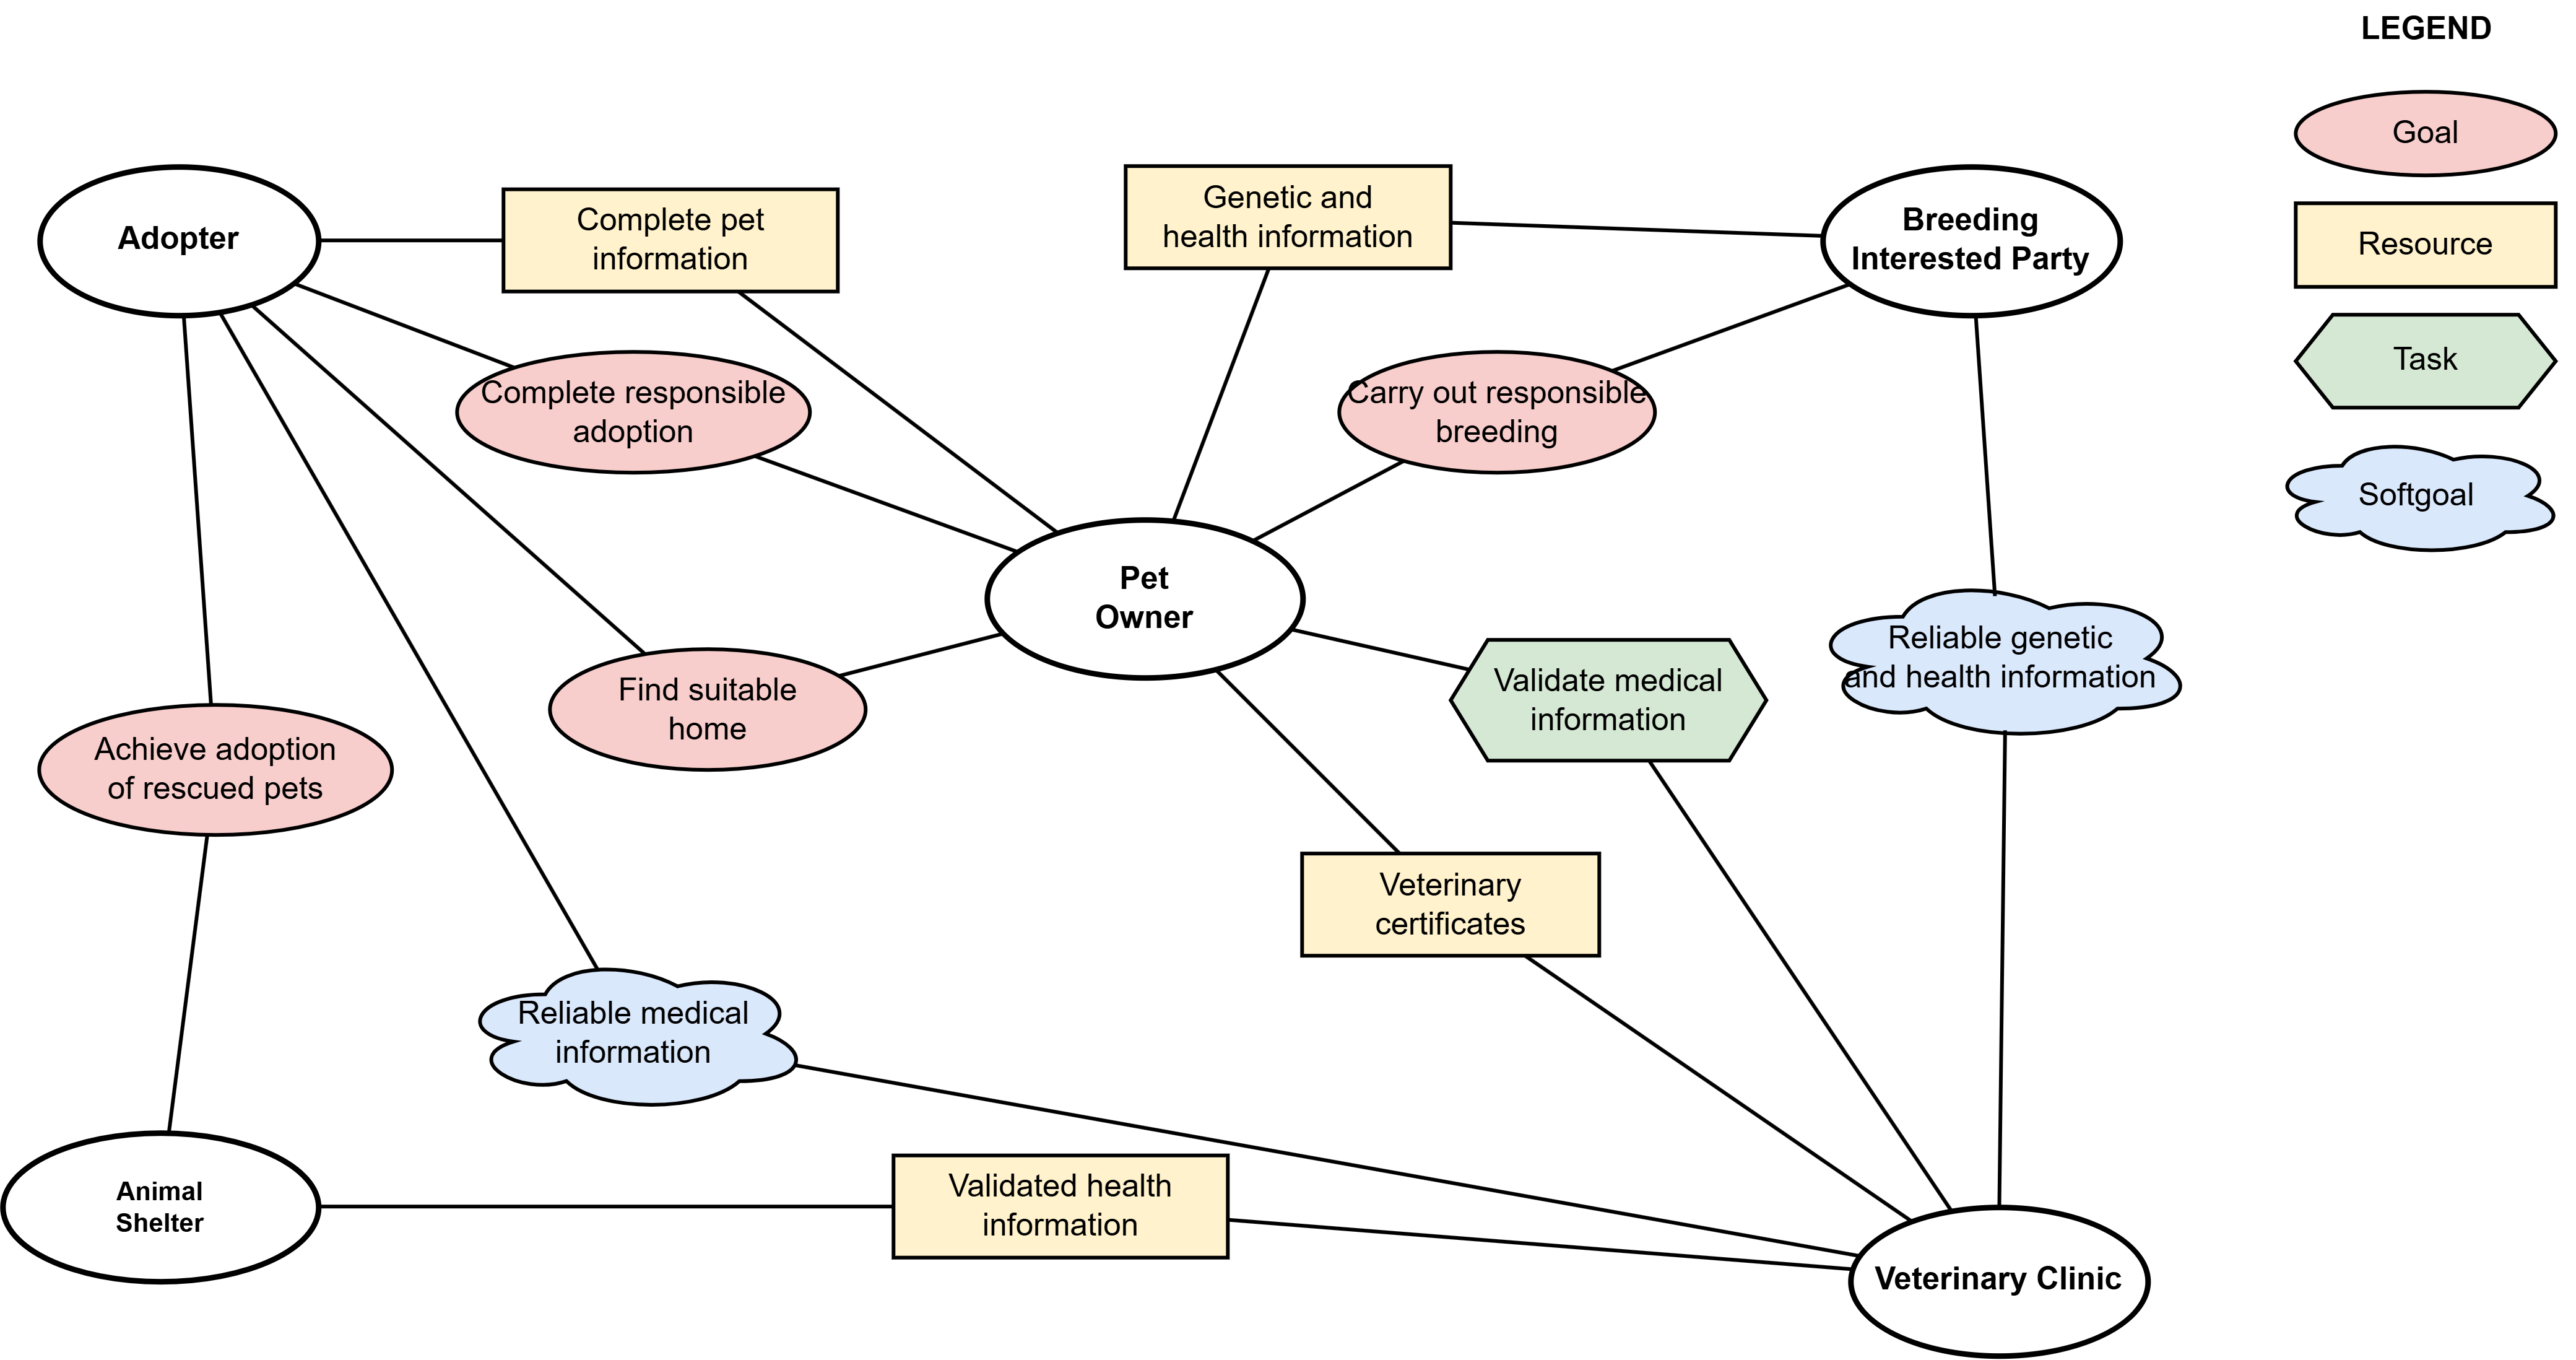
\includegraphics[width=1\textwidth]{figuras/DiagramaDeDependenciaEstrategica_MundiPets.png}
		\caption{Diagrama de dependencias estratégicas (SD) del sistema MundiPets.}
		\label{fig:contexto}
	\end{figure}
	
	Con el fin de representar gráficamente el límite del sistema descrito
	anteriormente, se presenta el diagrama contextual de MundiPets
	(Figura~\ref{fig:diagrama_contexto}), el cual ilustra al sistema como una caja
	única que recibe y envía información hacia los actores externos con los que
	interactúa, sin detallar los procesos internos que lo componen. Este diagrama
	permite visualizar de forma clara el alcance del sistema y los flujos de
	información que cruzan su frontera.
	
	\begin{figure}[H]
		\centering
		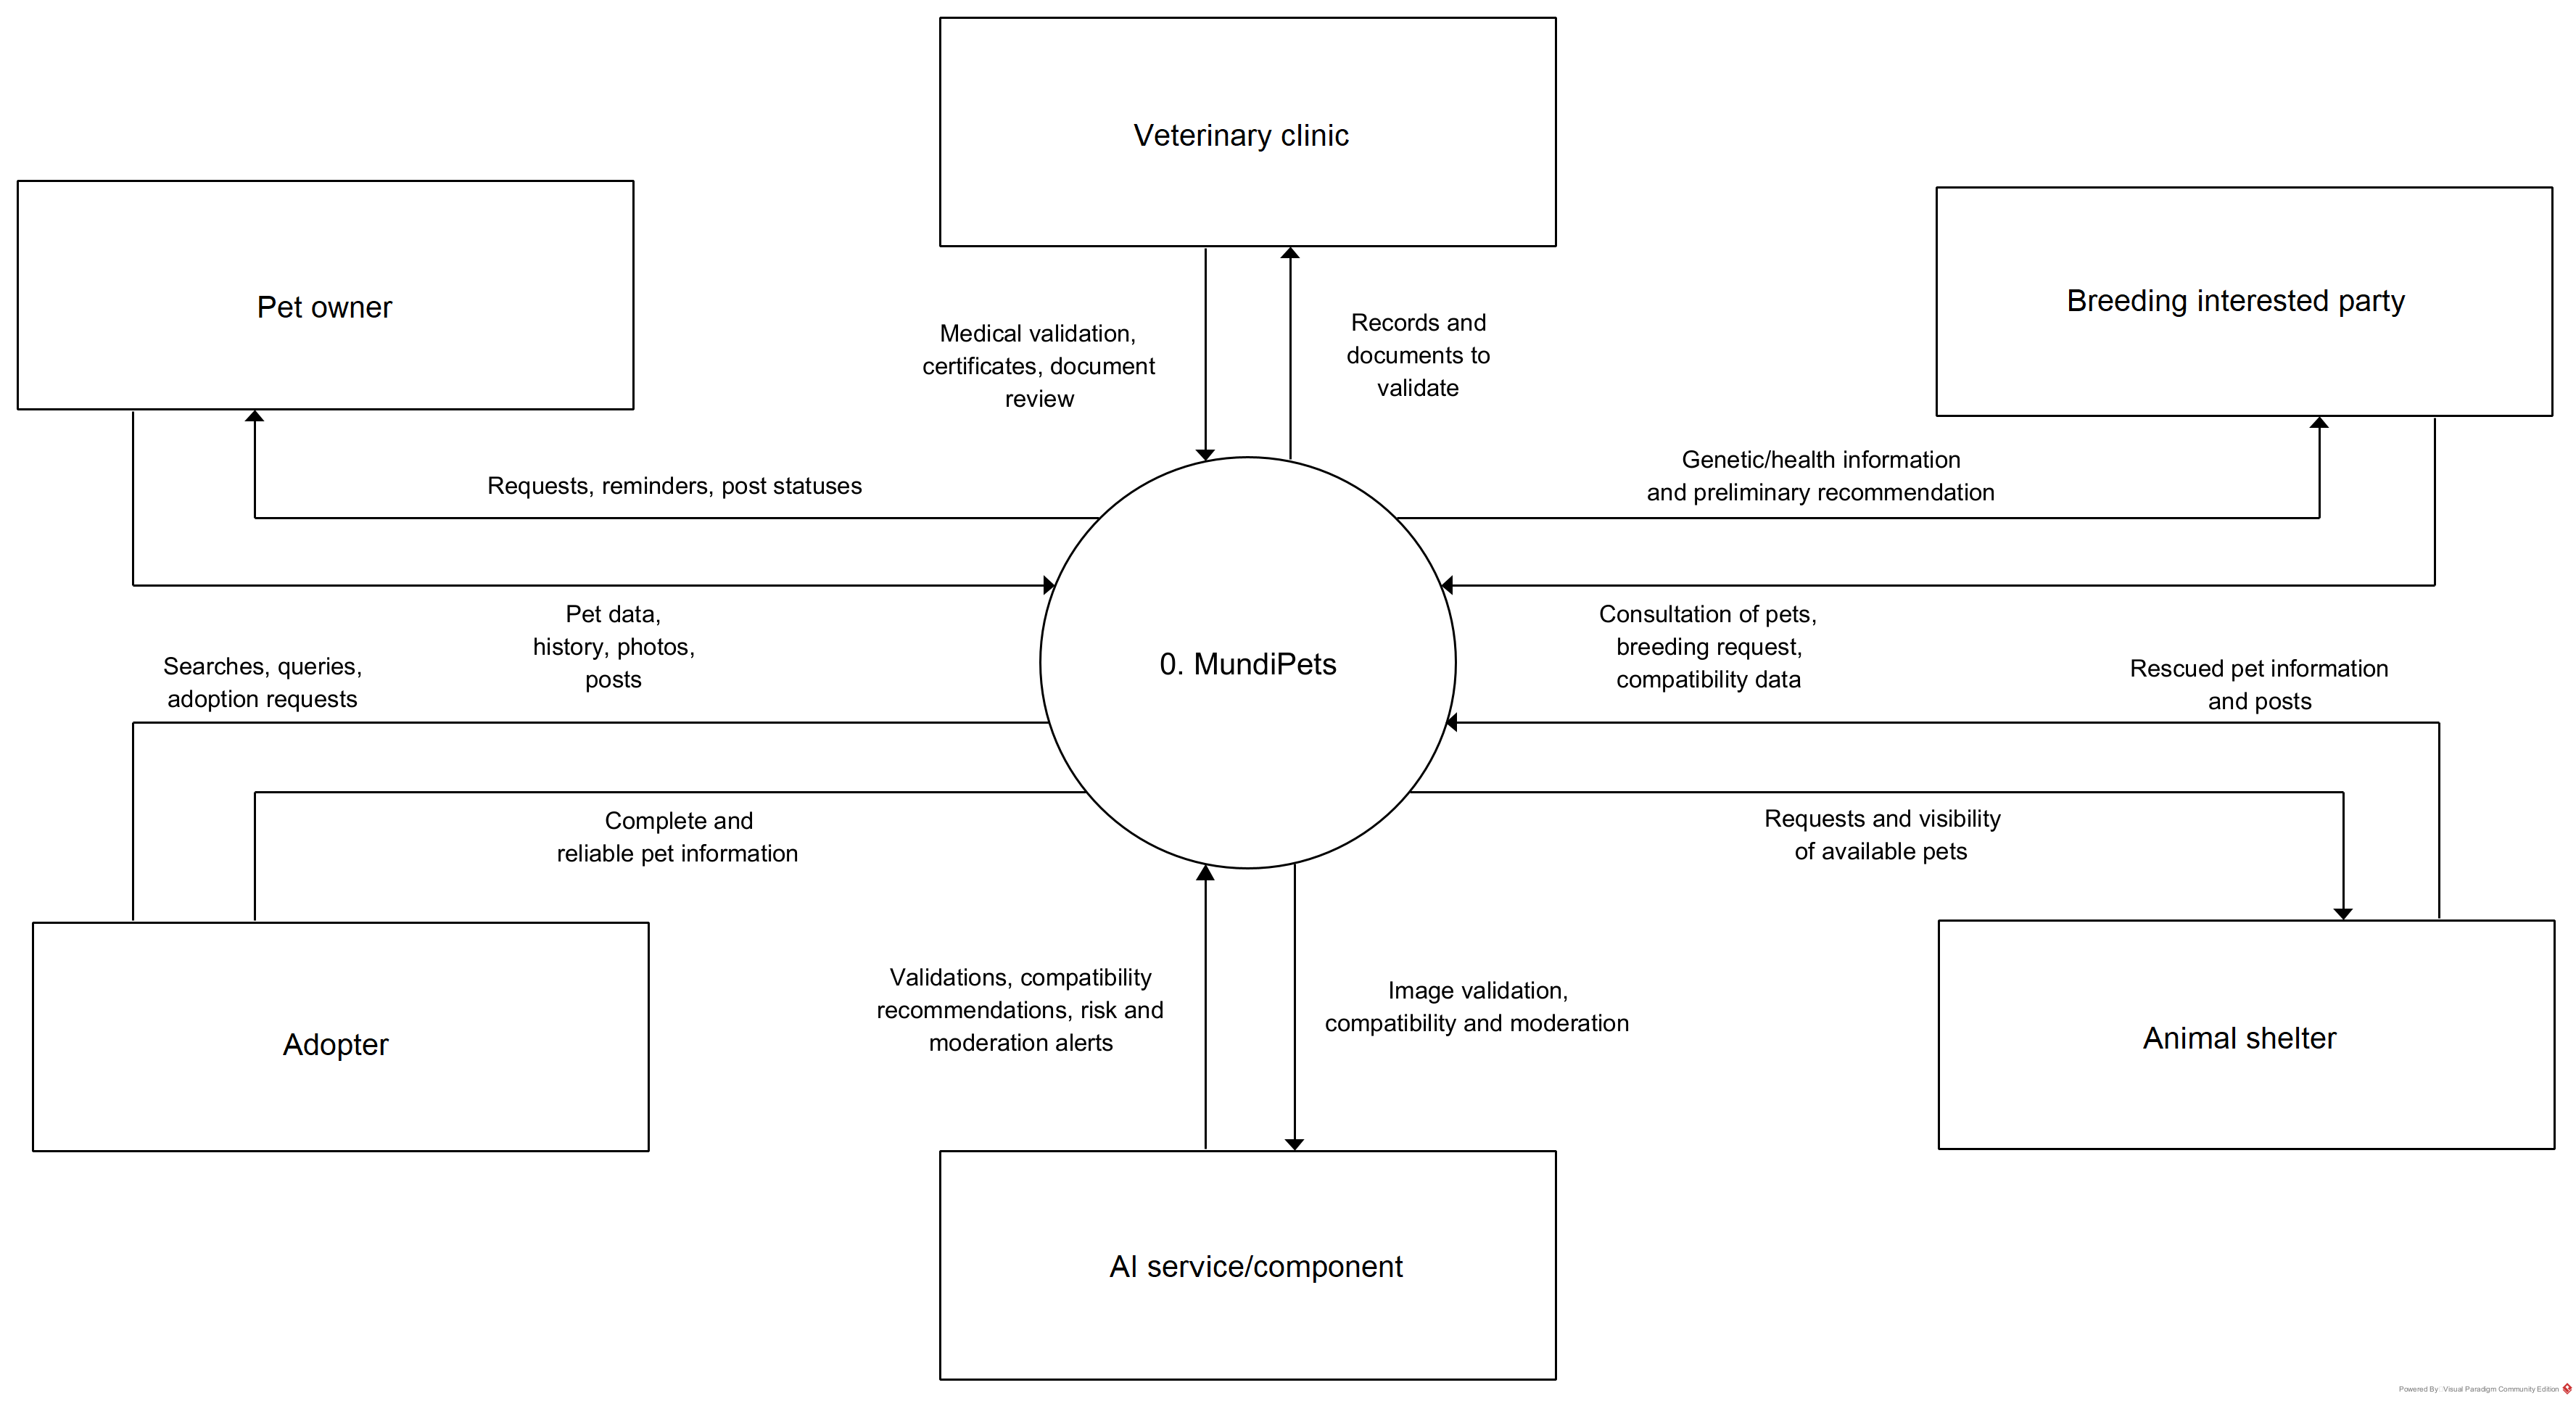
\includegraphics[width=1\textwidth]{figuras/DiagramaContexto_MundiPets.png}
		\caption{Diagrama contextual del sistema MundiPets.}
		\label{fig:diagrama_contexto}
	\end{figure}
	
	\subsection{Funciones del producto}
	\label{sec:funciones}
	
	A continuación se resumen, a alto nivel, las funciones principales que ofrece
	MundiPets, agrupadas por módulo:
	
	\begin{itemize}[leftmargin=*]
		\item \textbf{Gestión de perfiles de mascotas:} permite a los propietarios registrar, editar y publicar la información de sus mascotas (datos generales, historial médico, estado reproductivo).
		\item \textbf{Búsqueda y filtrado:} permite a adoptantes e interesados en cruza buscar mascotas disponibles según criterios como raza, edad, ubicación y propósito (adopción o cruza).
		\item \textbf{Publicación de disponibilidad:} permite a propietarios y refugios publicar mascotas disponibles para adopción o cruza responsable.
		\item \textbf{Validación de información médica:} permite que las veterinarias asociadas verifiquen y certifiquen la información sanitaria y genética cargada en el sistema.
		\item \textbf{Comunicación entre usuarios:} habilita el contacto entre propietario, adoptante e interesado en cruza para coordinar el proceso una vez identificado el interés mutuo.
		\item \textbf{Gestión de mascotas rescatadas:} permite a los refugios de animales publicar y dar seguimiento a mascotas rescatadas en proceso de adopción.
		\item \textbf{Reporte de conversaciones sospechosas:} permite a los usuarios reportar interacciones, mensajes o publicaciones que consideren fraudulentas, irresponsables o inapropiadas, fortaleciendo la seguridad y la confianza dentro de la plataforma.
		\item \textbf{Apoyo basado en inteligencia artificial:} incorpora funcionalidades de soporte orientadas a mejorar la calidad de la información publicada, la seguridad de las interacciones y la responsabilidad en los procesos de adopción y cruza, mediante alertas, recomendaciones preliminares y mecanismos de validación o moderación dentro de la plataforma. Estas funcionalidades no reemplazan la evaluación de profesionales veterinarios ni toman decisiones definitivas sobre la salud o reproducción de las mascotas.
	\end{itemize}
	
	\subsection{Clases y características de usuarios}
	\label{sec:perfiles}
	
	El sistema MundiPets está dirigido a diferentes clases de usuarios que
	participan en los procesos de registro de mascotas, adopción, cruza
	responsable y revisión de información sanitaria. Cada perfil tiene
	necesidades, funciones y niveles de acceso distintos, por lo que es necesario
	identificarlos de forma clara para definir correctamente los requisitos del
	sistema. Esta clasificación permite comprender qué acciones puede realizar
	cada usuario dentro de la plataforma y cómo se relaciona con los demás actores
	del sistema.
	
	\begin{longtable}{|p{2.2cm}|p{3.4cm}|p{3.4cm}|p{3.7cm}|p{1.2cm}|}
		\caption{Clases y características de usuarios del sistema MundiPets.} \label{tab:clases_usuario} \\
		\hline
		\textbf{Clase de usuario} & \textbf{Descripción del perfil} & \textbf{Necesidades principales} & \textbf{Funciones principales} & \textbf{Nivel de acceso} \\
		\hline
		\endfirsthead
		\hline
		\textbf{Clase de usuario} & \textbf{Descripción del perfil} & \textbf{Necesidades principales} & \textbf{Funciones principales} & \textbf{Nivel de acceso} \\
		\hline
		\endhead
		\hline
		\endfoot
		\hline
		\endlastfoot
		
		Propietario de mascota & Persona que registra y administra la información de su mascota dentro de MundiPets. Puede publicar su mascota para adopción o para un proceso de cruza responsable. & Necesita guardar datos completos de su mascota, actualizar su información, publicar su disponibilidad y revisar las solicitudes que recibe. & Crear y editar perfiles de mascotas, subir fotografías, registrar información médica básica, publicar mascotas para adopción o cruza, revisar solicitudes y comunicarse con otros usuarios. & Medio \\ \hline
		
		Adoptante & Persona interesada en encontrar una mascota para adoptar. Necesita información clara antes de tomar una decisión. & Necesita buscar mascotas disponibles, revisar sus datos principales, conocer su estado general y contactar al propietario o refugio. & Explorar mascotas disponibles, usar filtros de búsqueda, revisar perfiles, enviar solicitudes de adopción y comunicarse con propietarios o refugios. & Medio \\ \hline
		
		Interesado en cruza & Persona que busca una mascota compatible para realizar una cruza responsable. Requiere revisar información sanitaria y reproductiva antes de contactar al propietario. & Necesita consultar datos de salud, antecedentes, estado reproductivo y compatibilidad básica de la mascota. & Buscar mascotas disponibles para cruza, consultar perfiles, revisar información sanitaria referencial, enviar solicitudes de cruza y comunicarse con el propietario. & Medio \\ \hline
		
		Refugio de animales & Organización que registra y publica mascotas rescatadas para facilitar su adopción responsable. & Necesita dar visibilidad a las mascotas rescatadas, actualizar su disponibilidad, recibir solicitudes y comunicarse con posibles adoptantes. & Registrar mascotas rescatadas, publicar perfiles para adopción, actualizar estados, revisar solicitudes y comunicarse con adoptantes. & Alto \\ \hline
		
		Veterinaria & Profesional o entidad que revisa documentos e información sanitaria de las mascotas registradas en la plataforma. & Necesita revisar documentos autorizados, verificar información sanitaria referencial y registrar observaciones cuando sea necesario. & Revisar carnés o certificados veterinarios, validar o rechazar información sanitaria referencial y emitir observaciones dentro del sistema. & Alto \\ \hline
	\end{longtable}
	
	\subsection{Mapa de stakeholders}
	\label{sec:stakeholders}
	
	MundiPets involucra a diferentes stakeholders que influyen directa o
	indirectamente en el desarrollo del sistema. Cada uno tiene intereses,
	necesidades y niveles de participación distintos dentro del proyecto.
	Identificarlos permite comprender quiénes usarán la plataforma, quiénes
	aportan información para los requisitos, quiénes validan el contenido
	sanitario y quiénes supervisan el cumplimiento académico y técnico del
	documento ERS/SRS.
	
	\begin{longtable}{|p{1.8cm}|p{2.4cm}|p{1cm}|p{1cm}|p{3.7cm}|p{3.6cm}|}
		\caption{Mapa de stakeholders del sistema MundiPets.} \label{tab:matriz_stakeholders} \\
		\hline
		\textbf{Stakeholder} & \textbf{Interés en el sistema} & \textbf{Poder} & \textbf{Interés} & \textbf{Necesidades y expectativas} & \textbf{Estrategia de gestión} \\
		\hline
		\endfirsthead
		\hline
		\textbf{Stakeholder} & \textbf{Interés en el sistema} & \textbf{Poder} & \textbf{Interés} & \textbf{Necesidades y expectativas} & \textbf{Estrategia de gestión} \\
		\hline
		\endhead
		\hline
		\endfoot
		\hline
		\endlastfoot
		
		Propietario de mascota & Registrar y publicar información de sus mascotas para adopción o cruza responsable. & Medio & Alto & Crear perfiles completos, recibir solicitudes, comunicarse con interesados y mantener actualizada la información de sus mascotas. & Mantener informado y considerar sus necesidades en los requisitos de perfiles, publicaciones y solicitudes. \\ \hline
		
		Adoptante & Buscar mascotas disponibles para adopción con información clara y confiable. & Medio & Alto & Consultar perfiles, revisar datos básicos y sanitarios, aplicar filtros y enviar solicitudes de adopción. & Mantener informado y validar con este perfil las funciones de búsqueda, consulta y solicitud de adopción. \\ \hline
		
		Interesado en cruza & Encontrar mascotas compatibles para un proceso de cruza responsable. & Medio & Alto & Revisar información sanitaria, reproductiva y de comportamiento antes de contactar al propietario. & Mantener informado y considerar sus necesidades en los requisitos de cruza, compatibilidad y comunicación. \\ \hline
		
		Refugio de animales & Publicar mascotas rescatadas y facilitar procesos de adopción responsable. & Alto & Alto & Registrar varias mascotas, actualizar disponibilidad, recibir solicitudes y dar seguimiento a posibles adoptantes. & Gestionar de cerca, porque puede aportar reglas reales sobre adopción, seguimiento y publicación de mascotas rescatadas. \\ \hline
		
		Veterinarios & Revisar información sanitaria y documentos veterinarios registrados en la plataforma. & Alto & Alto & Validar información referencial, revisar carnés o certificados y registrar observaciones técnicas. & Gestionar de cerca mediante consultas sobre vacunas, documentos, salud animal y límites del sistema. \\ \hline
		
		Equipo desarrollador & Analizar, diseñar y documentar los requisitos del sistema MundiPets. & Alto & Alto & Contar con requisitos claros, viables, verificables y trazables para desarrollar el sistema. & Gestionar de cerca, asegurando comunicación constante, control de cambios y revisión técnica. \\ \hline
		
		Docente evaluador & Revisar el cumplimiento académico, metodológico y técnico de la ERS/SRS. & Alto & Alto & Verificar que el documento cumpla la estructura ERS/SRS, los mínimos solicitados y la trazabilidad. & Gestionar de cerca mediante revisión continua del documento, corrección de observaciones y cumplimiento de criterios. \\ \hline
	\end{longtable}
	
	\subsubsection{Matriz poder/interés}
	\label{sec:poder-interes}
	
	\begin{longtable}{|p{3.0cm}|p{1.4cm}|p{1.4cm}|p{3.8cm}|p{4.2cm}|}
		\caption{Matriz poder/interés de stakeholders del sistema MundiPets.} \label{tab:clasificacion_stakeholders} \\
		\hline
		\textbf{Stakeholder} & \textbf{Poder} & \textbf{Interés} & \textbf{Clasificación} & \textbf{Estrategia} \\
		\hline
		\endfirsthead
		\hline
		\textbf{Stakeholder} & \textbf{Poder} & \textbf{Interés} & \textbf{Clasificación} & \textbf{Estrategia} \\
		\hline
		\endhead
		\hline
		\endfoot
		\hline
		\endlastfoot
		
		Refugio de animales & Alto & Alto & Actor clave & Gestionar de cerca \\ \hline
		
		Veterinarios & Alto & Alto & Actor clave técnico & Gestionar de cerca \\ \hline
		
		Equipo desarrollador & Alto & Alto & Actor técnico principal & Gestionar de cerca \\ \hline
		
		Docente evaluador & Alto & Alto & Actor académico clave & Gestionar de cerca \\ \hline
		
		Propietario de mascota & Medio & Alto & Usuario principal & Mantener informado y consultar \\ \hline
		
		Adoptante & Medio & Alto & Usuario principal & Mantener informado y consultar \\ \hline
		
		Interesado en cruza & Medio & Alto & Usuario principal & Mantener informado y consultar \\ \hline
	\end{longtable}
	
	\subsubsection{Conflictos potenciales entre stakeholders}
	\label{sec:conflictos}
	
	\begin{longtable}{|p{2.2cm}|p{2.2cm}|p{2.8cm}|p{3.2cm}|p{3.3cm}|}
		\caption{Conflictos potenciales entre stakeholders del sistema MundiPets.} \label{tab:matriz_conflictos} \\
		\hline
		\textbf{Conflicto potencial} & \textbf{Stakeholders involucrados} & \textbf{Causa del conflicto} & \textbf{Impacto posible en el sistema} & \textbf{Estrategia de gestión} \\
		\hline
		\endfirsthead
		\hline
		\textbf{Conflicto potencial} & \textbf{Stakeholders involucrados} & \textbf{Causa del conflicto} & \textbf{Impacto posible en el sistema} & \textbf{Estrategia de gestión} \\
		\hline
		\endhead
		\hline
		\endfoot
		\hline
		\endlastfoot
		
		Publicación de información incompleta de mascotas & Propietario de mascota, adoptante y refugio. & Algunos usuarios pueden publicar mascotas sin datos suficientes sobre salud, edad, comportamiento o disponibilidad. & Decisiones de adopción o cruza con información incompleta, menor confianza en la plataforma y aumento de solicitudes mal gestionadas. & Definir campos obligatorios, mostrar alertas de perfil incompleto y permitir revisión por el refugio cuando corresponda. \\ \hline
		
		Confianza en la información sanitaria & Propietario de mascota, veterinaria, adoptante e interesado en cruza. & La información médica puede ser registrada por usuarios sin respaldo documental. & Riesgo de que adoptantes o interesados en cruza tomen decisiones con datos poco confiables. & Solicitar documentos veterinarios, permitir validación sanitaria referencial y mostrar el estado de revisión de cada documento. \\ \hline
		
		Privacidad de datos personales y médicos & Propietario, adoptante, interesado en cruza y veterinaria. & Algunos usuarios pueden querer ver más información de la permitida, especialmente datos médicos o de contacto. & Exposición innecesaria de datos sensibles y pérdida de confianza en el sistema. & Definir permisos por rol, limitar datos visibles y permitir acceso solo a la información necesaria según el proceso. \\ \hline
		
		Cruza irresponsable o mal interpretada & Propietario de mascota, interesado en cruza y veterinaria. & Los usuarios pueden interpretar la compatibilidad como autorización definitiva para realizar una cruza. & Riesgos sanitarios, reproductivos o éticos si se realiza una cruza sin revisión profesional. & Aclarar que la plataforma solo ofrece información referencial y recomendar validación veterinaria antes de cualquier decisión. \\ \hline
		
		Diferencias entre necesidades de usuarios y alcance académico & Docente evaluador, equipo desarrollador y usuarios potenciales. & Los usuarios pueden esperar más funciones de las que el proyecto puede desarrollar en esta fase. & Sobrecarga de requisitos, aumento del alcance y dificultad para cumplir la entrega. & Mantener documentado el alcance, clasificar funciones futuras como mejora posterior y priorizar requisitos esenciales. \\ \hline
		
		Validación documental limitada & Veterinaria y propietario de mascota. & La veterinaria puede revisar documentos, pero no reemplaza una consulta médica ni una historia clínica oficial. & Confusión sobre el valor legal o clínico de la validación realizada en la plataforma. & Usar el término ``validación referencial'', no ``certificación clínica'', y aclarar los límites del sistema. \\ \hline
		
		Comunicación inadecuada entre usuarios & Propietario, adoptante e interesado en cruza. & Pueden generarse mensajes fuera de tema, spam, lenguaje ofensivo o acuerdos externos no controlados. & Disminución de la confianza, reportes frecuentes y uso inadecuado de la plataforma. & Incorporar reglas de comunicación, advertencias sobre acuerdos externos y mecanismos básicos para reportar interacciones inadecuadas. \\ \hline
	\end{longtable}
	
	\subsection{Entorno operativo}
	\label{sec:entorno}
	
	MundiPets opera como una aplicación web responsiva, accesible desde
	navegadores de escritorio y dispositivos móviles, sin requerir instalación
	adicional por parte del usuario final.
	
	\textbf{Requisitos del lado del cliente:}
	\begin{itemize}[leftmargin=*]
		\item Navegador web actualizado (Google Chrome, Mozilla Firefox, Microsoft Edge o Safari, en sus versiones recientes).
		\item Conexión a internet estable (mínimo 1 Mbps) para la carga de imágenes y sincronización de datos.
		\item Dispositivo con pantalla táctil o mouse/teclado (smartphone, tablet o computador).
	\end{itemize}
	
	\textbf{Requisitos del lado del servidor:}
	\begin{itemize}[leftmargin=*]
		\item Servidor con soporte para alojamiento web (hosting propio o servicio en la nube).
		\item Base de datos relacional o no relacional según la tecnología seleccionada en la fase de diseño.
		\item Almacenamiento para archivos multimedia (fotografías de mascotas y certificados veterinarios).
	\end{itemize}
	
	Estos requisitos se ajustan al contexto real de uso, en el cual tanto los
	propietarios de mascotas como las veterinarias consultadas acceden
	habitualmente a internet mediante teléfonos inteligentes. Para el Producto
	Mínimo Viable (Sección~\ref{sec:mvp}), el entorno operativo se acota a un
	despliegue local reproducible mediante contenedores, sin necesidad de
	infraestructura de producción.
	
	\subsection{Suposiciones y dependencias}
	\label{sec:suposiciones}
	
	\textbf{Suposiciones:}
	\begin{itemize}[leftmargin=*]
		\item Se asume que los propietarios de mascotas y las veterinarias consultadas cuentan con acceso regular a internet.
		\item Se asume que las veterinarias aliadas estarán dispuestas a validar la información médica cargada por los propietarios, según lo expresado en las entrevistas realizadas.
		\item Se asume que los usuarios proporcionarán información veraz sobre sus mascotas al momento del registro.
		\item Se asume que el volumen inicial de usuarios permitirá operar con una infraestructura básica de hosting durante la primera fase del proyecto.
	\end{itemize}
	
	\textbf{Dependencias externas:}
	\begin{itemize}[leftmargin=*]
		\item El sistema depende de veterinarias externas para la validación y certificación de la información médica y sanitaria de las mascotas (ver diagrama de dependencias, Figura~\ref{fig:contexto}).
		\item El sistema depende de refugios de animales como fuente de información sobre mascotas rescatadas disponibles para adopción.
		\item Podría requerirse la integración con un servicio externo de notificaciones (correo electrónico o mensajería) para alertar a los usuarios sobre nuevas coincidencias o mensajes.
		\item El sistema depende de un proveedor de hosting/almacenamiento en la nube para el despliegue y la persistencia de archivos multimedia.
	\end{itemize}
	
	\subsection{Modelado organizacional en i*}
	\label{sec:istar}
	
	El lenguaje i* \cite{yu1995} modela la intencionalidad de los actores
	organizacionales mediante dos diagramas complementarios. El Diagrama de
	Dependencia Estratégica (SD) muestra qué depende cada actor de los demás sin
	detallar su estructura interna; el Diagrama de Razón Estratégica (SR) abre el
	interior de cada actor y expone sus metas, metas blandas, tareas y recursos.
	
	\subsubsection{Diagrama de Dependencia Estratégica (SD)}
	\label{sec:istar-sd}
	
	La Figura~\ref{fig:contexto} (Sección~\ref{sec:perspectiva}) corresponde al
	Diagrama de Dependencia Estratégica del sistema MundiPets. En él, el
	propietario de mascota depende del sistema para encontrar un adoptante o un
	interesado en cruza adecuado; el adoptante y el interesado en cruza dependen
	del sistema para obtener información confiable sobre las mascotas publicadas;
	la veterinaria actúa como fuente externa de confianza al validar y certificar
	la información médica; y el refugio de animales depende del sistema como
	canal de visibilidad para las mascotas rescatadas. Estas dependencias
	delimitan el conjunto de actores que después se abren en el Diagrama de
	Razón Estratégica.
	
	\subsubsection{Diagrama de Razón Estratégica (SR)}
	\label{sec:istar-sr}
	
	La Figura~\ref{fig:sr} presenta el Diagrama de Razón Estratégica para los tres
	actores principales del sistema: la Veterinaria, el Propietario de mascota y
	el Adoptante/Interesado en cruza.
	
	\begin{figure}[H]
		\centering
		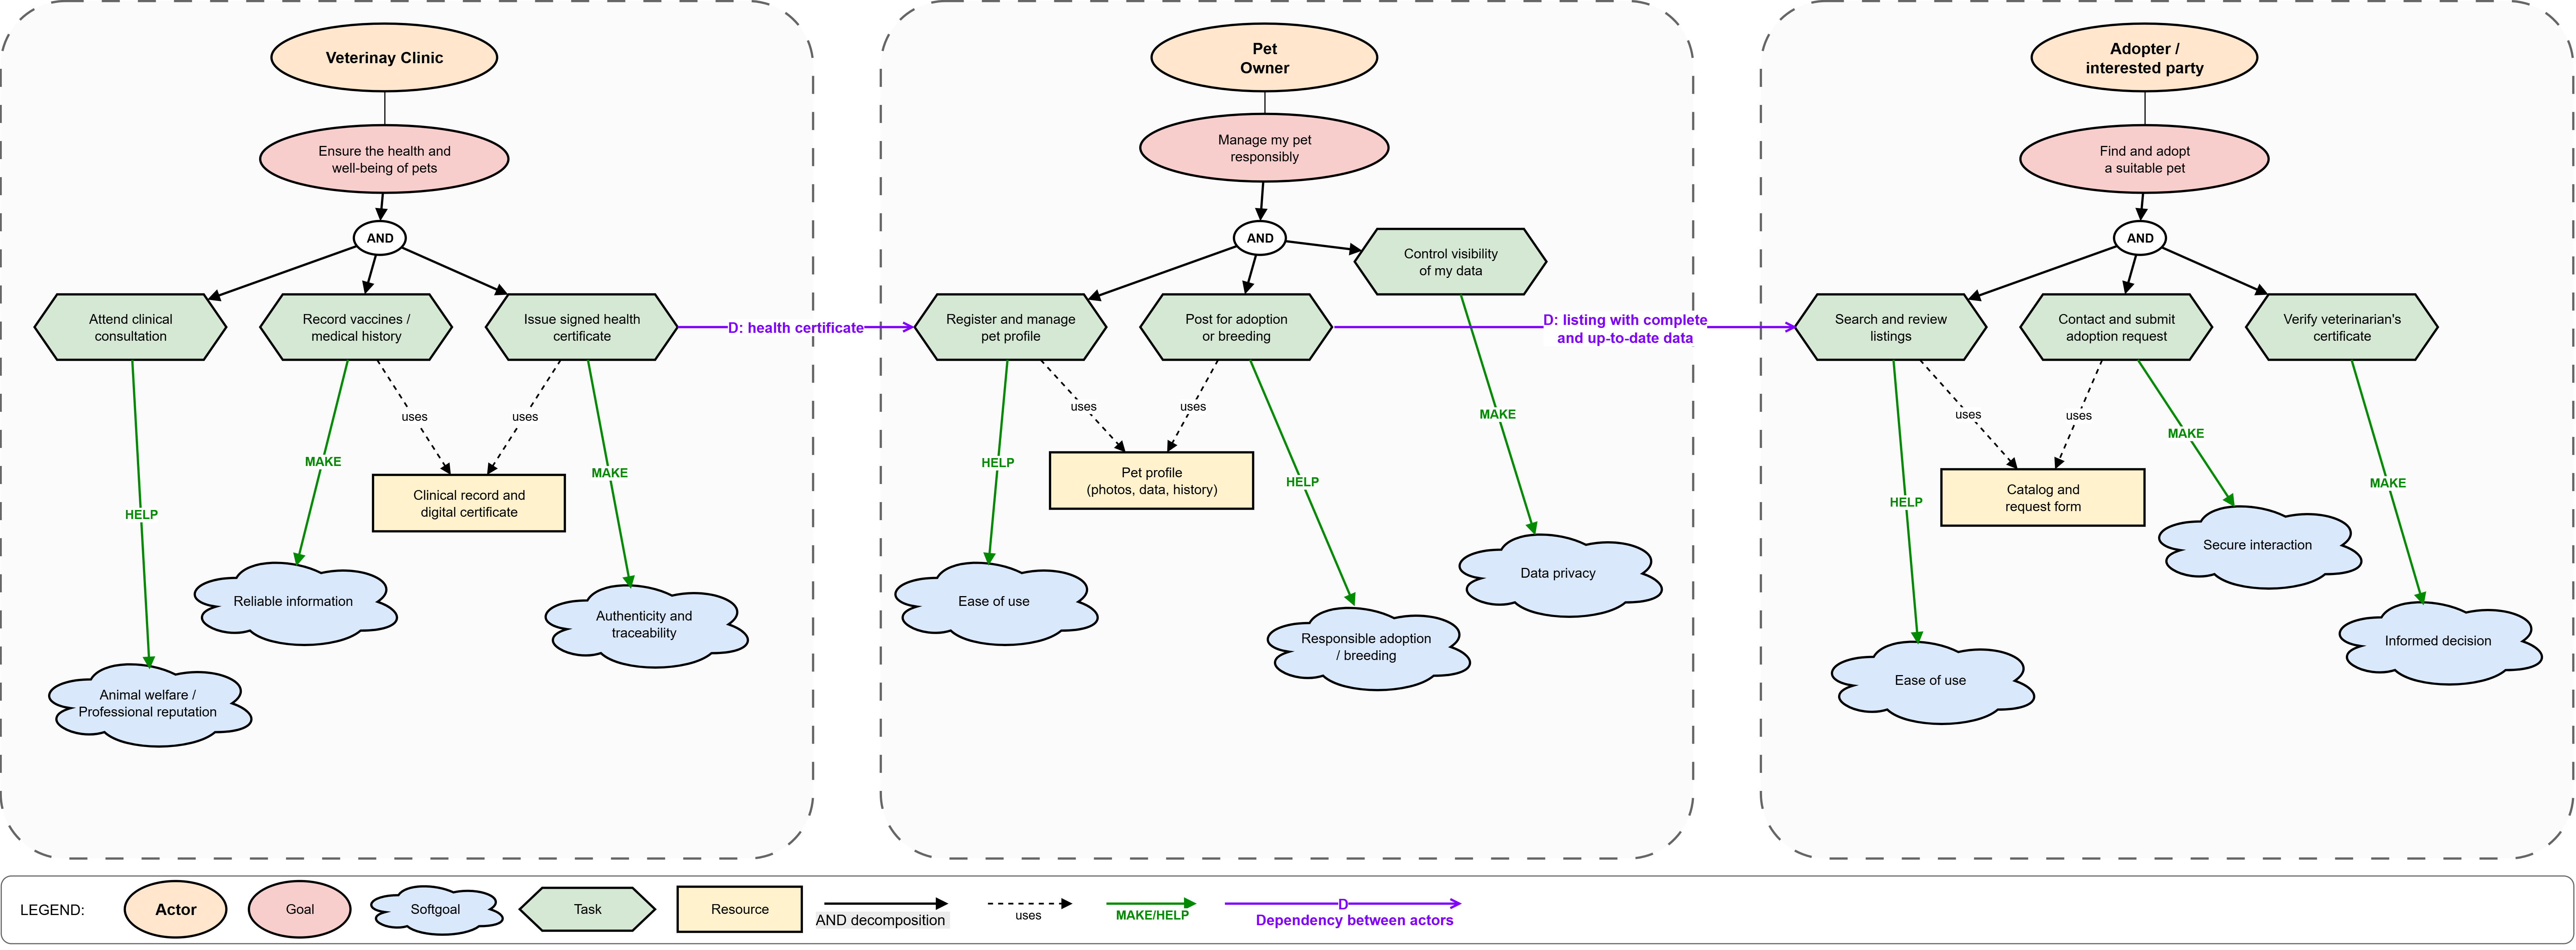
\includegraphics[width=1\textwidth]{figuras/DiagramaDeRazonEstrategica_MundiPets.png}
		\caption{Diagrama de Razón Estratégica (SR) del sistema MundiPets.}
		\label{fig:sr}
	\end{figure}
	
	Para el actor \textbf{Veterinaria}, la meta \emph{garantizar la salud y el
		bienestar de las mascotas} se descompone (mediante descomposición AND) en tres
	tareas: atender la consulta clínica, registrar vacunas e historial médico, y
	emitir el certificado sanitario firmado. Las dos últimas tareas producen los
	recursos \emph{registro clínico y certificado digital}, que a su vez alimentan
	la dependencia de tipo recurso \enquote{certificado de salud} hacia el actor
	Propietario de mascota. Estas tareas contribuyen positivamente a las metas
	blandas \emph{bienestar animal / reputación profesional},
	\emph{información confiable} y \emph{autenticidad y trazabilidad}, conectando
	directamente con RNF-05 (integridad de la información médica) y con el
	requisito legal de minimización de datos sanitarios.
	
	Para el actor \textbf{Propietario de mascota}, la meta \emph{gestionar mi
		mascota de forma responsable} se descompone en las tareas registrar y
	administrar el perfil de la mascota, publicar en adopción o cruza, y
	controlar la visibilidad de mis datos. Las dos primeras tareas usan el
	recurso compartido \emph{perfil de mascota (fotos, datos, historial)} y
	contribuyen a las metas blandas \emph{facilidad de uso} y
	\emph{adopción/cruza responsable}; la tarea de control de visibilidad
	contribuye a la meta blanda \emph{privacidad de los datos}, y la publicación
	del perfil alimenta la dependencia de tipo recurso \enquote{publicación con
		datos completos y actualizados} hacia el actor Adoptante/Interesado en cruza.
	Estas metas blandas se conectan con RNF-01 (protección de la información) y
	RNF-04 (facilidad de uso de la plataforma).
	
	Para el actor \textbf{Adoptante/Interesado en cruza}, la meta \emph{encontrar
		y adoptar una mascota adecuada} se descompone en buscar y revisar
	publicaciones, contactar y enviar una solicitud de adopción o cruza, y
	verificar el certificado de la veterinaria. Las dos primeras tareas usan el
	recurso \emph{catálogo y formulario de solicitud} y contribuyen a las metas
	blandas \emph{facilidad de uso} e \emph{interacción segura}; la verificación
	del certificado contribuye a la meta blanda \emph{decisión informada}, que se
	conecta con RNF-06 (exactitud del componente de inteligencia artificial de
	evaluación de compatibilidad) y con los requisitos de explicabilidad de la
	Sección~\ref{sec:explicabilidad}.
	
	El SR evidencia así cómo las metas blandas de los tres actores --
	\emph{información confiable}, \emph{privacidad de los datos} e
	\emph{interacción segura}, entre otras -- no son aspiraciones abstractas, sino
	que se materializan en los requisitos no funcionales concretos definidos en la
	Sección~\ref{sec:rnf}.
	
	% ############################################################
	%           SECCION 3 -- REQUISITOS ESPECIFICOS COMPLETOS
	% ############################################################
	\section{Requisitos específicos completos}
	\label{sec:requisitos}
	
	\subsection{Interfaces externas}
	\label{sec:interfaces}
	
	Esta sección describe las interfaces a través de las cuales el sistema
	MundiPets interactúa con sus usuarios, con el hardware sobre el que se
	ejecuta y con los servicios de software externos de los que depende,
	siguiendo la estructura recomendada por ISO/IEC/IEEE 29148:2018
	\cite{iso29148}.
	
	\subsubsection{Interfaz de usuario (mockups de alta fidelidad)}
	\label{sec:mockups}
	
	Esta subsección presenta los mockups de alta fidelidad correspondientes a
	las interfaces de usuario que soportan los requisitos funcionales de
	prioridad \emph{Debe tener} del sistema MundiPets. Cada mockup se identifica
	con un código MU-XX, se describe brevemente en función de la interacción que
	representa y se vincula explícitamente con los requisitos funcionales (RF)
	que soporta, en cumplimiento de la trazabilidad exigida por el estándar
	ISO/IEC/IEEE 29148:2018 \cite{iso29148}.
	
	El prototipo navegable completo, elaborado en Figma, se encuentra disponible
	en el siguiente enlace:
	
	\begin{center}
		\small\url{https://www.figma.com/proto/EHp0XoVnL5SNnt8SSFy8AO/Mockups---MundiPets?node-id=20-3}
	\end{center}
	
	\paragraph{MU-01: Crear cuenta}
	
	En la Figura~\ref{fig:mu01} se muestra el mockup de la interfaz de registro y
	verificación de identidad, punto de entrada para los cuatro roles de usuario
	que interactúan con la plataforma (propietario, adoptante, interesado en
	cruza y veterinaria). El formulario solicita los datos de identificación
	básicos y permite adjuntar el documento requerido para la verificación,
	mostrando al usuario el estado de verificación resultante antes de
	habilitarlo para participar en procesos de adopción o cruza.
	
	\textbf{RF asociados:} RF-12.
	
	\begin{figure}[H]
		\centering
		
\includegraphics[width=0.55\textwidth]{{figuras/MU-01_Crear cuenta}.png}
		\caption{Mockup MU-01: Crear cuenta.}
		\label{fig:mu01}
	\end{figure}
	
	\paragraph{MU-02: Registrar mascota}
	
	Este mockup representa el formulario mediante el cual el propietario ingresa
	la información general de una nueva mascota (nombre, especie, raza, sexo,
	edad y estado reproductivo) junto con sus fotografías de identificación. La
	interfaz agrupa los campos obligatorios de forma secuencial y valida su
	completitud antes de habilitar el registro definitivo del perfil dentro de
	la plataforma.
	
	\textbf{RF asociados:} RF-01.
	
	\begin{figure}[H]
		\centering
		
\includegraphics[width=0.62\textwidth]{{figuras/MU-02_Registrar mascota}.png}
		\caption{Mockup MU-02: Registrar mascota.}
		\label{fig:mu02}
	\end{figure}
	
	\paragraph{MU-03: Agenda veterinaria y validación documental}
	
	Este mockup muestra el panel exclusivo para veterinarias, organizado por
	fechas y estados de revisión (pendientes, en revisión, validadas y
	rechazadas). Permite calendarizar la revisión de la documentación sanitaria
	y del carnet de vacunación cargados por los propietarios, y emitir el
	dictamen de validación referencial correspondiente dentro del sistema,
	dejando constancia de la observación técnica en caso de rechazo.
	
	\textbf{RF asociados:} RF-09, RF-14.
	
	\begin{figure}[H]
		\centering
		
\includegraphics[width=0.75\textwidth]{{figuras/MU-03_Agenda Veterinaria y Validación Documental}.png}
		\caption{Mockup MU-03: Agenda veterinaria y validación documental.}
		\label{fig:mu03}
	\end{figure}
	
	\paragraph{MU-04: Feed de publicaciones (búsqueda y filtrado)}
	
	En este mockup se presenta la interfaz que despliega las mascotas
	disponibles en un formato de tarjetas visuales, acompañada de un panel de
	filtros dinámicos (tipo de mascota, estado de interés y ubicación
	aproximada). Permite al adoptante o interesado en cruza refinar la búsqueda
	y seleccionar una tarjeta para acceder al perfil detallado de la mascota o
	iniciar una solicitud.
	
	\textbf{RF asociados:} RF-03, RF-04.
	
	\begin{figure}[H]
		\centering
		
\includegraphics[width=0.75\textwidth]{{figuras/MU-04_Feed de publicaciones (Búsqueda y filtrado)}.png}
		\caption{Mockup MU-04: Feed de publicaciones (búsqueda y filtrado).}
		\label{fig:mu04}
	\end{figure}
	
	\paragraph{MU-05: Solicitud de adopción o cruza}
	
	Este mockup representa el formulario interactivo mediante el cual el usuario
	interesado formaliza su solicitud de adopción o cruza responsable sobre una
	mascota publicada. Incluye la selección del tipo de solicitud, un campo de
	justificación obligatorio, la aceptación explícita de los términos de
	bienestar animal y un canal de mensajería directa que se habilita con el
	propietario una vez enviada la solicitud. La misma pantalla aloja, mediante
	secciones secundarias que se activan según el estado de la solicitud, dos
	funcionalidades adicionales que no requieren una pantalla propia: el
	indicador de etapa del flujo de adopción por etapas (RF-18), que muestra en
	qué punto de \emph{EnEntrevista}, \emph{EnVisita} o \emph{EnPeriodoDePrueba}
	se encuentra la solicitud una vez aceptada, y el canal de seguimiento
	post-adopción (RF-22), que reutiliza el mismo hilo de mensajería para el
	contacto entre propietario original y adoptante tras completarse la
	adopción.
	
	\textbf{RF asociados:} RF-05, RF-07, RF-08, RF-18, RF-22.
	
	\begin{figure}[H]
		\centering
		
\includegraphics[width=0.75\textwidth]{{figuras/MU-05_Solicitud de adopción o cruza}.png}
		\caption{Mockup MU-05: Solicitud de adopción o cruza.}
		\label{fig:mu05}
	\end{figure}
	
	\paragraph{MU-06: Perfil de mascota}
	
	En este mockup se muestra la vista de perfil completo de una mascota, que
	centraliza su identidad general, la información sanitaria referencial
	(vacunas, desparasitación y certificado veterinario) y su estado de
	disponibilidad para adopción o cruza. La interfaz distingue el estado de
	vigencia de cada dato sanitario mediante indicadores visuales y ofrece un
	acceso directo para contactar al propietario.
	
	\textbf{RF asociados:} RF-01, RF-02, RF-03, RF-13, RF-16.
	
	\begin{figure}[H]
		\centering
		
\includegraphics[width=0.42\textwidth]{{figuras/MU-06_Perfil de mascota}.png}
		\caption{Mockup MU-06: Perfil de mascota.}
		\label{fig:mu06}
	\end{figure}
	
	\paragraph{MU-07: Evaluación de compatibilidad}
	
	Este mockup representa la interfaz mediante la cual el propietario o el
	interesado en cruza selecciona dos mascotas registradas para obtener una
	recomendación preliminar de compatibilidad. La pantalla presenta ambos
	perfiles de forma comparativa, el resultado generado por el componente de
	inteligencia artificial y su explicación causal asociada, junto con la
	advertencia de que el resultado es orientativo y no sustituye la evaluación
	de un profesional veterinario. Cuando el resultado detecta una condición de
	riesgo sanitario o físico en la interacción evaluada, la misma pantalla
	despliega, como aviso contextual superpuesto al resultado, la alerta de
	riesgo exigida por RF-23, sin requerir una pantalla propia adicional.
	
	\textbf{RF asociados:} RF-06, RF-23.
	
	\begin{figure}[H]
		\centering
		
\includegraphics[width=0.68\textwidth]{{figuras/MU-07_Evaluacion de compatibilidad}.png}
		\caption{Mockup MU-07: Evaluación de compatibilidad.}
		\label{fig:mu07}
	\end{figure}
	
	\paragraph{MU-08: Configuración de privacidad de la mascota}
	
	En este mockup se muestra la interfaz mediante la cual el propietario
	administra la visibilidad de la información sensible asociada a su mascota y
	a su propio perfil, tales como la ubicación, los datos de contacto y
	afecciones médicas específicas. Cada categoría de dato sensible cuenta con
	un control independiente de nivel de visibilidad, permitiendo restringir el
	acceso a usuarios no autorizados sin afectar la información obligatoria para
	la validación veterinaria.
	
	\textbf{RF asociados:} RF-11.
	
	\begin{figure}[H]
		\centering
		
\includegraphics[width=0.48\textwidth]{{figuras/MU-08_Configuracion de privacidad de la mascota}.png}
		\caption{Mockup MU-08: Configuración de privacidad de la mascota.}
		\label{fig:mu08}
	\end{figure}
	
	\paragraph{Especificación y trazabilidad de interfaces de usuario}
	
	La Tabla~\ref{tab:trazabilidad_mockups} presenta la matriz de especificación
	y trazabilidad de las interfaces de usuario de MundiPets, detallando los
	códigos de los mockups, las pantallas, los actores, el flujo secuencial de
	acceso y su vinculación directa con los requisitos funcionales (RF) para
	garantizar la trazabilidad del sistema.
	
	{\footnotesize
		\begin{longtable}{@{}L{1.5cm} L{2.0cm} L{2.3cm} L{3.2cm} L{2.0cm} L{2.9cm}@{}}
			\caption{Matriz de especificación y trazabilidad de las interfaces de usuario.}
			\label{tab:trazabilidad_mockups}\\
			\toprule
			\textbf{ID Mockup} & \textbf{Interfaz} & \textbf{Usuario principal} & \textbf{Flujo de navegación} & \textbf{RF vinculados} & \textbf{Justificación} \\
			\midrule
			\endfirsthead
			\multicolumn{6}{@{}l}{\small\itshape (continuación)}\\
			\toprule
			\textbf{ID Mockup} & \textbf{Interfaz} & \textbf{Usuario principal} & \textbf{Flujo de navegación} & \textbf{RF vinculados} & \textbf{Justificación} \\
			\midrule
			\endhead
			\bottomrule
			\endlastfoot
			MU-01 & Crear cuenta & Propietario / Adoptante / Interesado en cruza / Veterinaria & Landing $\rightarrow$ \enquote{Crear cuenta} $\rightarrow$ Formulario de registro $\rightarrow$ Verificación de identidad & RF-12 & Formaliza el registro y la verificación de identidad exigida antes de participar en procesos de adopción o cruza. \\
			\addlinespace
			MU-02 & Registrar mascota & Propietario de mascota & Dashboard $\rightarrow$ Mis Mascotas $\rightarrow$ \enquote{Agregar mascota} $\rightarrow$ Formulario de datos generales & RF-01 & Captura los datos básicos y fotográficos que dan origen al perfil de la mascota dentro de la plataforma. \\
			\addlinespace
			MU-03 & Agenda veterinaria y validación documental & Veterinaria & Dashboard $\rightarrow$ Validaciones $\rightarrow$ Agenda de revisiones $\rightarrow$ Detalle del documento & RF-09, RF-14 & Organiza cronológicamente la revisión de documentos sanitarios y del carnet de vacunación por parte de un profesional autorizado. \\
			\addlinespace
			MU-04 & Feed de publicaciones (búsqueda y filtrado) & Adoptante / Interesado en cruza & Menú principal $\rightarrow$ Explorar Mascotas $\rightarrow$ Filtros dinámicos & RF-03, RF-04 & Presenta el catálogo de mascotas disponibles mediante tarjetas visuales y filtros de búsqueda combinables. \\
			\addlinespace
			MU-05 & Solicitud de adopción o cruza & Adoptante / Interesado en cruza & Feed de publicaciones $\rightarrow$ Tarjeta de mascota $\rightarrow$ Botón \enquote{Solicitar} $\rightarrow$ Formulario de solicitud & RF-05, RF-07, RF-08, RF-18, RF-22 & Formaliza el interés sobre una mascota, recopila la justificación del solicitante, abre el canal de mensajería con el propietario y aloja, en secciones secundarias, el indicador de etapa del flujo de adopción y el seguimiento post-adopción. \\
			\addlinespace
			MU-06 & Perfil de mascota & Propietario / Adoptante / Interesado en cruza & Feed de publicaciones $\rightarrow$ Tarjeta de mascota $\rightarrow$ Ver perfil completo & RF-01, RF-02, RF-03, RF-13, RF-16 & Centraliza la identidad, el historial médico referencial y los antecedentes genéticos de la mascota para sustentar decisiones de adopción o cruza. \\
			\addlinespace
			MU-07 & Evaluación de compatibilidad & Propietario de mascota / Interesado en cruza & Perfil de mascota $\rightarrow$ \enquote{Evaluar compatibilidad} $\rightarrow$ Selección de segunda mascota $\rightarrow$ Resultado & RF-06, RF-23 & Presenta el resultado comparativo generado por el componente de inteligencia artificial junto con su explicación causal y, cuando corresponde, la alerta de riesgo superpuesta al resultado, sin sustituir la evaluación veterinaria. \\
			\addlinespace
			MU-08 & Configuración de privacidad de la mascota & Propietario de mascota & Dashboard $\rightarrow$ Configuración $\rightarrow$ Privacidad de mi mascota & RF-11 & Permite al propietario definir qué información sensible (ubicación, contacto, afecciones específicas) es visible para otros usuarios. \\
		\end{longtable}
	}
	
	Los ocho mockups cubren la totalidad de los quince requisitos funcionales
	de prioridad \emph{Must}: doce con una pantalla dedicada, y los tres
	restantes --- RF-18 (flujo de adopción por etapas), RF-22 (seguimiento
	post-adopción) y RF-23 (alertas de riesgo) --- asociados formalmente a un
	mockup ya existente, indicado explícitamente en su \emph{RF asociados}
	(Sección~\ref{sec:mockups}), en lugar de requerir una pantalla nueva:
	RF-18 y RF-22 quedan asociados a MU-05, donde se resuelven como una
	sección secundaria que muestra la etapa de la solicitud (RF-18) y el hilo
	de mensajería reutilizado para el seguimiento (RF-22); y RF-23 queda
	asociado a MU-07, donde se despliega como una alerta contextual
	superpuesta al resultado de la evaluación de compatibilidad. Ningún RF de
	prioridad \emph{Must} queda, por tanto, sin un mockup que lo soporte,
	aunque tres de ellos lo compartan con otro RF en lugar de tener una
	pantalla exclusiva. Esta asociación queda trazada en el Apéndice~D
	(columna Estado de la traza). Los requisitos funcionales de prioridad
	\emph{Should} y \emph{Could} (RF-04, RF-07, RF-10, RF-15, RF-17, RF-19 a
	RF-21 y RF-24 a RF-27) se apoyan de la misma manera sobre las pantallas ya
	existentes mediante secciones secundarias, conforme al alcance del
	Producto Mínimo Viable definido en la Sección~\ref{sec:mvp-alcance}.
	
	\subsubsection{Interfaz de hardware}
	\label{sec:interfaz-hardware}
	
	MundiPets es una aplicación web responsiva que no requiere hardware
	especializado ni controladores propietarios; toda la interacción con los
	dispositivos se realiza a través de las API estándar expuestas por el
	navegador, en coherencia con el entorno operativo descrito en la
	Sección~\ref{sec:entorno} y con la portabilidad exigida por RNF-11. Las
	interfaces de hardware relevantes son las siguientes:
	
	\begin{itemize}[leftmargin=*]
		\item \textbf{Cámara y almacenamiento local del dispositivo.} Se accede
		mediante el selector de archivos y la API \texttt{MediaDevices} del
		navegador para capturar o adjuntar las fotografías de la mascota (RF-01)
		y los documentos veterinarios digitalizados (RF-14). El sistema no accede
		al hardware fuera de la acción explícita del usuario.
		\item \textbf{Servicios de geolocalización.} Se emplea la
		\texttt{Geolocation API} del navegador, previa autorización del usuario,
		para derivar la zona aproximada de la mascota. La ubicación exacta nunca
		se almacena ni se muestra, conforme a RNF-16 y a la configuración de
		privacidad de RF-11.
		\item \textbf{Pantalla y dispositivos de entrada.} La interfaz se adapta a
		pantallas táctiles y a la combinación de teclado y ratón, con un diseño
		responsivo verificable en resoluciones de teléfono inteligente, tableta y
		computador de escritorio (RNF-04, RNF-11).
		\item \textbf{Conectividad de red.} Se requiere una conexión a internet
		estable de al menos 1\,Mbps para la carga de imágenes y la sincronización
		de datos; el sistema no define ninguna interfaz de red propietaria.
		\item \textbf{Infraestructura del lado del servidor.} No se impone hardware
		específico: el despliegue se realiza sobre servidores virtualizados o
		contenedores en un proveedor de nube, de acuerdo con la escalabilidad
		horizontal exigida por RNF-12.
	\end{itemize}
	
	\subsubsection{Interfaz de software}
	\label{sec:interfaz-software}
	
	El sistema se comunica con componentes y servicios externos a través de
	interfaces de software bien delimitadas. La Tabla~\ref{tab:interfaz_software}
	resume cada interfaz, su propósito, el mecanismo de intercambio previsto y
	los requisitos que la sustentan.
	
	{\footnotesize
		\begin{longtable}{@{}L{3.2cm} L{4.5cm} L{3.4cm} L{3.4cm}@{}}
			\caption{Interfaces de software del sistema MundiPets.}
			\label{tab:interfaz_software}\\
			\toprule
			\textbf{Interfaz externa} & \textbf{Propósito} & \textbf{Mecanismo de intercambio} & \textbf{Requisitos asociados} \\
			\midrule
			\endfirsthead
			\multicolumn{4}{@{}l}{\small\itshape (continuación)}\\
			\toprule
			\textbf{Interfaz externa} & \textbf{Propósito} & \textbf{Mecanismo de intercambio} & \textbf{Requisitos asociados} \\
			\midrule
			\endhead
			\bottomrule
			\endlastfoot
			Navegador web del cliente & Renderizado de la interfaz de usuario y consumo de los servicios de la aplicación & HTTPS sobre HTML5, CSS3 y JavaScript; respuestas en JSON & RNF-04, RNF-11 \\
			\addlinespace
			Componente de evaluación de compatibilidad (IA) & Generar el resultado orientativo de cruza y su explicación causal & API interna REST/JSON expuesta por el módulo de IA (Sección~\ref{sec:componentes}) & RF-06, RNF-06, RNF-13, RD-01 \\
			\addlinespace
			Componente de validación de imágenes (IA) & Verificar que la fotografía corresponde a una mascota y es apropiada & API interna REST/JSON & RF-17, RNF-07, RNF-14 \\
			\addlinespace
			Componente de moderación de mensajes (IA) & Clasificar el contenido de los mensajes antes de su entrega & API interna REST/JSON & RF-07, RNF-15 \\
			\addlinespace
			WhatsApp Business API & Envío de recordatorios de controles preventivos y notificaciones & API REST del proveedor sobre HTTPS, con canal de respaldo \emph{in-app} & RF-10, RNF-09, RD-08 \\
			\addlinespace
			Servicio de correo electrónico & Confirmación de cuenta, recuperación de contraseña y avisos del sistema & SMTP o API del proveedor sobre canal cifrado & RF-12, RNF-09 \\
			\addlinespace
			Sistema gestor de base de datos & Persistencia de la información transaccional del sistema & Conexión cifrada mediante el controlador del SGBD seleccionado & RNF-01, RNF-05, RNF-12 \\
			\addlinespace
			Almacenamiento de archivos multimedia & Persistencia de fotografías de mascotas y documentos veterinarios & API de almacenamiento de objetos sobre HTTPS, con URL firmadas de acceso temporal & RF-01, RF-14, RNF-01, RD-04 \\
		\end{longtable}
	}
	
	Todas las comunicaciones con servicios externos se realizan sobre canales
	cifrados y transmiten únicamente los datos estrictamente necesarios para la
	operación solicitada, en cumplimiento del principio de minimización de datos
	de la LOPDP recogido en la Sección~\ref{sec:legales} y de la restricción de
	diseño RD-04. Cuando un servicio externo no se encuentre disponible, el
	sistema degrada la funcionalidad de forma controlada --- por ejemplo,
	sustituyendo la notificación por mensajería con una notificación interna ---
	sin interrumpir el resto de la operación, según lo previsto en RD-08.
	
	% ------------------------------------------------------------
	\subsection{Requisitos funcionales}
	\label{sec:rf}
	
	Los requisitos funcionales se especifican con los ocho atributos exigidos por la
	plantilla de la asignatura, aplicando las recomendaciones de redacción de
	ISO/IEC/IEEE 29148:2018 \cite{iso29148}.
	
	\subsubsection{RF-01 --- Registrar mascota}
	
	\begin{atributos}{RF-01}{RF-01 --- Registrar mascota.}
		Identificador & RF-01 \\
		Nombre & Registrar mascota \\
		Descripción & El sistema deberá permitir al propietario registrar una mascota ingresando su información general, incluyendo nombre, especie, raza, sexo, edad, estado reproductivo y fotografías para su identificación dentro de la plataforma. \\
		Actor & Propietario de mascota \\
		Origen (ID de evidencia) & EV-02, EV-03, EV-05, EV-06, EV-07, EV-08 \\
		Entradas & Nombre, especie, raza, sexo, edad, estado reproductivo, fotografías, descripción. \\
		Salidas & Perfil de mascota registrado correctamente. \\
		Precondiciones & El propietario debe estar autenticado en el sistema. \\
		Postcondiciones & La mascota queda almacenada y disponible para futuras consultas, adopciones o procesos de cruza. \\
		Prioridad (MoSCoW) & Must \\
		Criterio de verificación & Registrar una mascota con datos válidos y comprobar que el perfil queda almacenado y puede consultarse posteriormente. \\
	\end{atributos}
	
	\subsubsection{RF-02 --- Gestionar historial médico de la mascota}
	
	\begin{atributos}{RF-02}{RF-02 --- Gestionar historial médico de la mascota.}
		Identificador & RF-02 \\
		Nombre & Gestionar historial médico de la mascota \\
		Descripción & El sistema deberá permitir registrar el historial médico de una mascota, incluyendo desparasitaciones, enfermedades, alergias, cirugías, tratamientos y controles veterinarios. \\
		Actor & Propietario de mascota, Veterinaria \\
		Origen (ID de evidencia) & EV-01, EV-02, EV-03, EV-04, EV-05, EV-06, EV-07, EV-15, EV-16 \\
		Entradas & Desparasitaciones, enfermedades, alergias, cirugías, tratamientos, controles médicos, observaciones. \\
		Salidas & Historial médico actualizado. \\
		Precondiciones & La mascota debe estar registrada en el sistema. \\
		Postcondiciones & El historial médico queda actualizado y disponible para usuarios autorizados. \\
		Prioridad (MoSCoW) & Must \\
		Criterio de verificación & Registrar nuevos antecedentes médicos y verificar que aparecen correctamente dentro del historial clínico de la mascota. \\
	\end{atributos}
	
	\subsubsection{RF-03 --- Consultar perfil completo de una mascota}
	
	\begin{atributos}{RF-03}{RF-03 --- Consultar perfil completo de una mascota.}
		Identificador & RF-03 \\
		Nombre & Consultar perfil completo de una mascota \\
		Descripción & El sistema deberá permitir visualizar el perfil completo de una mascota mostrando su información general, historial médico autorizado, fotografías, comportamiento, vacunas, edad, raza para procesos de adopción o cruza. \\
		Actor & Propietario de mascota, Adoptante, Interesado en cruza \\
		Origen (ID de evidencia) & EV-02, EV-04, EV-05, EV-06, EV-07, EV-14 \\
		Entradas & Identificador de la mascota. \\
		Salidas & Perfil completo de la mascota. \\
		Precondiciones & La mascota debe existir y el usuario debe tener permisos para visualizar la información correspondiente. \\
		Postcondiciones & El usuario obtiene la información necesaria para tomar decisiones sobre adopción o cruza. \\
		Prioridad (MoSCoW) & Must \\
		Criterio de verificación & Consultar una mascota registrada y comprobar que se muestra toda la información autorizada. \\
	\end{atributos}
	
	\subsubsection{RF-04 --- Buscar y filtrar mascotas}
	
	\begin{atributos}{RF-04}{RF-04 --- Buscar y filtrar mascotas.}
		Identificador & RF-04 \\
		Nombre & Buscar y filtrar mascotas \\
		Descripción & El sistema deberá permitir buscar mascotas aplicando filtros como especie, raza, edad, ubicación, estado de salud, tamaño, temperamento y disponibilidad para adopción o cruza. \\
		Actor & Adoptante, Interesado en cruza \\
		Origen (ID de evidencia) & EV-07, EV-08 \\
		Entradas & Criterios de búsqueda y filtros seleccionados. \\
		Salidas & Lista de mascotas que cumplen los criterios establecidos. \\
		Precondiciones & Deben existir mascotas registradas en la plataforma. \\
		Postcondiciones & Se muestran únicamente las mascotas que cumplen los filtros aplicados. \\
		Prioridad (MoSCoW) & Should \\
		Criterio de verificación & Aplicar diferentes filtros, incluidos tamaño y temperamento, y comprobar que los resultados corresponden con los criterios seleccionados. \\
	\end{atributos}
	
	\subsubsection{RF-05 --- Gestionar solicitudes de adopción}
	
	\begin{atributos}{RF-05}{RF-05 --- Gestionar solicitudes de adopción.}
		Identificador & RF-05 \\
		Nombre & Gestionar solicitudes de adopción \\
		Descripción & El sistema deberá permitir que un usuario interesado envíe una solicitud de adopción, incluyendo su fotografía de perfil, y que el propietario la acepte o rechace en una primera revisión, con base en la información del solicitante. \\
		Actor & Adoptante, Propietario de mascota \\
		Origen (ID de evidencia) & EV-01, EV-02, EV-03, EV-05, EV-06, EV-08 \\
		Entradas & Solicitud de adopción, información y fotografía del solicitante. \\
		Salidas & Solicitud registrada y estado de aceptación o rechazo de la revisión inicial. \\
		Precondiciones & La mascota debe estar disponible para adopción. \\
		Postcondiciones & La solicitud queda registrada como aceptada o rechazada en su revisión inicial; si es aceptada, continúa su ciclo de vida conforme al flujo por etapas de RF-18. \\
		Prioridad (MoSCoW) & Must \\
		Criterio de verificación & Registrar una solicitud y comprobar que el propietario puede visualizar el perfil del solicitante y gestionarla correctamente. \\
	\end{atributos}
	
	\subsubsection{RF-06 --- Evaluar compatibilidad entre mascotas para cruza}
	
	\begin{atributos}{RF-06}{RF-06 --- Evaluar compatibilidad entre mascotas para cruza.}
		Identificador & RF-06 \\
		Nombre & Evaluar compatibilidad entre mascotas para cruza \\
		Descripción & El sistema deberá evaluar la compatibilidad entre dos mascotas registradas para procesos de cruza, considerando su raza, edad, estado de salud, antecedentes genéticos, parentesco, comportamiento e historial médico. \\
		Actor & Propietario de mascota, Interesado en cruza \\
		Origen (ID de evidencia) & EV-01 a EV-08, EV-11, EV-13, EV-14, EV-15, EV-16 \\
		Entradas & Selección de dos mascotas registradas. \\
		Salidas & Veredicto de compatibilidad en tres niveles discretos --- \emph{compatible}, \emph{compatible con reservas} o \emph{no recomendado}---, acompañado de la explicación exigida por RNF-13 y de una advertencia de que el resultado es orientativo y no sustituye la evaluación de un veterinario. \\
		Precondiciones & Ambas mascotas deben encontrarse registradas. \\
		Postcondiciones & El usuario dispone de un veredicto clasificado y de su explicación para decidir si continúa con el proceso de cruza. \\
		Prioridad (MoSCoW) & Must \\
		Criterio de verificación & Seleccionar dos mascotas y comprobar que el sistema presenta uno de los tres niveles de veredicto junto con la explicación y la advertencia orientativa. \\
	\end{atributos}
	
	
	\subsubsection{RF-07 --- Sistema de mensajería entre usuarios}
	
	\begin{atributos}{RF-07}{RF-07 --- Sistema de mensajería entre usuarios.}
		Identificador & RF-07 \\
		Nombre & Sistema de mensajería entre usuarios \\
		Descripción & El sistema deberá permitir la comunicación entre propietarios e interesados mediante mensajes para coordinar procesos de adopción y cruza, incluyendo la posibilidad de que el usuario reporte un mensaje o interacción como spam, lenguaje ofensivo o intento de acuerdo externo indebido, registrando el motivo del reporte asociado a la conversación. \\
		Actor & Propietario de mascota, Adoptante, Interesado en cruza \\
		Origen (ID de evidencia) & EV-02, EV-07, EV-08 \\
		Entradas & Mensaje enviado por un usuario; motivo de reporte manual seleccionado por el receptor. \\
		Salidas & Conversación registrada entre los usuarios; reporte manual registrado y asociado a la conversación cuando corresponde. \\
		Precondiciones & Ambos usuarios deben encontrarse registrados. \\
		Postcondiciones & El mensaje queda almacenado y disponible para ambos participantes; si se reporta, el motivo queda vinculado a la conversación para su revisión. \\
		Prioridad (MoSCoW) & Could \\
		Criterio de verificación & Enviar un mensaje entre dos usuarios y verificar que ambos puedan visualizarlo; reportar un mensaje y comprobar que el motivo quede asociado a la conversación. \\
	\end{atributos}
	

	\subsubsection{RF-08 --- Gestionar solicitudes de cruza}
	
	\begin{atributos}{RF-08}{RF-08 --- Gestionar solicitudes de cruza.}
		Identificador & RF-08 \\
		Nombre & Gestionar solicitudes de cruza \\
		Descripción & El sistema deberá permitir que los propietarios soliciten procesos de cruza entre mascotas y que el propietario de la otra mascota pueda aceptar o rechazar la solicitud con base en la información disponible. \\
		Actor & Propietario de mascota, Interesado en cruza \\
		Origen (ID de evidencia) & EV-01, EV-02, EV-03, EV-05, EV-06, EV-07 \\
		Entradas & Solicitud de cruza, identificación de ambas mascotas. \\
		Salidas & Solicitud registrada con estado pendiente, aceptada o rechazada. \\
		Precondiciones & Ambas mascotas deben estar registradas y disponibles para cruza. \\
		Postcondiciones & La solicitud queda almacenada y actualizada con el estado correspondiente. \\
		Prioridad (MoSCoW) & Must \\
		Criterio de verificación & Registrar una solicitud de cruza y verificar que el propietario receptor pueda aceptarla o rechazarla correctamente. \\
	\end{atributos}
	
	\subsubsection{RF-09 --- Validar la información médica de una mascota}
	
	\begin{atributos}{RF-09}{RF-09 --- Validar la información médica de una mascota.}
		Identificador & RF-09 \\
		Nombre & Validar la información médica de una mascota \\
		Descripción & El sistema deberá permitir que una veterinaria autorizada valide la información médica registrada de una mascota, indicando que los datos han sido verificados por un profesional. \\
		Actor & Veterinaria \\
		Origen (ID de evidencia) & EV-03, EV-05, EV-07, EV-15, EV-16 \\
		Entradas & Historial médico, carnet de vacunación, controles veterinarios y documentos clínicos. \\
		Salidas & Información médica validada con su respectiva identificación de verificación. \\
		Precondiciones & La mascota debe encontrarse registrada y disponer de información médica cargada en el sistema. \\
		Postcondiciones & La información médica queda marcada como validada por una veterinaria autorizada. \\
		Prioridad (MoSCoW) & Must \\
		Criterio de verificación & Validar el historial médico de una mascota y comprobar que el sistema muestre el estado de información validada. \\
	\end{atributos}
	
	\subsubsection{RF-10 --- Gestionar recordatorios de controles preventivos}
	
	\begin{atributos}{RF-10}{RF-10 --- Gestionar recordatorios de controles preventivos.}
		Identificador & RF-10 \\
		Nombre & Gestionar recordatorios de controles preventivos \\
		Descripción & El sistema deberá entregar al propietario, con una semana y un día de anticipación, un recordatorio sobre próximas vacunas, desparasitaciones y controles veterinarios de la mascota, utilizando WhatsApp como canal principal y el canal de notificación in-app como respaldo automático cuando el proveedor externo no esté disponible \\
		Actor & Propietario de mascota \\
		Origen (ID de evidencia) & EV-02, EV-04, EV-06, EV-11 \\
		Entradas & Fechas de vacunas, controles veterinarios y desparasitaciones; estado de disponibilidad del proveedor externo de mensajería. \\
		Salidas & Notificaciones o recordatorios generados por el sistema en los dos momentos definidos, por WhatsApp o, en su ausencia, por el canal in-app de respaldo. \\
		Precondiciones & Deben existir fechas registradas para los controles preventivos de la mascota. \\
		Postcondiciones & El propietario recibe el recordatorio correspondiente antes de la fecha programada, por al menos uno de los dos canales disponibles. \\
		Prioridad (MoSCoW) & Should \\
		Criterio de verificación & Registrar una fecha de vacunación próxima y verificar que el sistema genere el recordatorio una semana y un día antes; simular la indisponibilidad de WhatsApp y comprobar que el recordatorio se entregue igualmente por el canal in-app. \\
	\end{atributos}
	
	
	\subsubsection{RF-11 --- Administrar la privacidad de la información}
	
	\begin{atributos}{RF-11}{RF-11 --- Administrar la privacidad de la información.}
		Identificador & RF-11 \\
		Nombre & Administrar la privacidad de la información \\
		Descripción & El sistema deberá permitir que el propietario determine qué información de su mascota y de su perfil podrá ser visualizada por otros usuarios, protegiendo los datos considerados sensibles (ubicación, datos de contacto y afecciones específicas). \\
		Actor & Propietario de mascota \\
		Origen (ID de evidencia) & EV-02, EV-05, EV-06, EV-07, EV-08, EV-09, EV-10, EV-14, EV-18 \\
		Entradas & Configuración de privacidad seleccionada por el propietario. \\
		Salidas & Permisos de visualización actualizados. \\
		Precondiciones & El propietario debe encontrarse autenticado en el sistema. \\
		Postcondiciones & La información se muestra únicamente a los usuarios autorizados según la configuración establecida. \\
		Prioridad (MoSCoW) & Must \\
		Criterio de verificación & Modificar la configuración de privacidad y comprobar que la información restringida no sea visible para usuarios no autorizados. \\
	\end{atributos}
	
	\subsubsection{RF-12 --- Verificar la identidad de los usuarios}
	
	\begin{atributos}{RF-12}{RF-12 --- Verificar la identidad de los usuarios.}
		Identificador & RF-12 \\
		Nombre & Verificar la identidad de los usuarios \\
		Descripción & El sistema deberá verificar la identidad de los usuarios mediante la carga y validación de un documento de identidad oficial y vigente, antes de habilitar su participación en procesos de adopción o cruza. \\
		Actor & Propietario de mascota, Adoptante, Interesado en cruza \\
		Origen (ID de evidencia) & EV-01, EV-03, EV-07, EV-08, EV-09 \\
		Entradas & Documento de identidad oficial (imagen o escaneo), datos personales asociados. \\
		Salidas & Usuario verificado dentro de la plataforma. \\
		Precondiciones & El usuario debe haber iniciado el proceso de registro. \\
		Postcondiciones & El usuario obtiene el estado de identidad verificada. \\
		Prioridad (MoSCoW) & Must \\
		Criterio de verificación & Registrar un usuario cargando un documento de identidad válido y comprobar que el sistema lo marca como verificado; cargar un documento inválido o ilegible y comprobar que el sistema lo rechaza. \\
	\end{atributos}
	
	\subsubsection{RF-13 --- Registrar publicaciones de mascotas}
	
	\begin{atributos}{RF-13}{RF-13 --- Registrar publicaciones de mascotas.}
		Identificador & RF-13 \\
		Nombre & Registrar publicaciones de mascotas \\
		Descripción & El sistema deberá permitir al propietario publicar una mascota indicando si estará disponible para adopción, cruza o ambas opciones, incluyendo toda la información autorizada del perfil de la mascota. \\
		Actor & Propietario de mascota \\
		Origen (ID de evidencia) & EV-01, EV-02, EV-04, EV-06, EV-07, EV-08 \\
		Entradas & Tipo de publicación, fotografías, descripción y disponibilidad. \\
		Salidas & Publicación visible para otros usuarios. \\
		Precondiciones & La mascota debe estar registrada en el sistema. \\
		Postcondiciones & La mascota queda publicada según el tipo de proceso seleccionado. \\
		Prioridad (MoSCoW) & Must \\
		Criterio de verificación & Publicar una mascota y comprobar que aparezca correctamente en el listado de adopciones o cruzas. \\
	\end{atributos}
	
	\subsubsection{RF-14 --- Gestionar carnet de vacunación}
	
	\begin{atributos}{RF-14}{RF-14 --- Gestionar carnet de vacunación.}
		Identificador & RF-14 \\
		Nombre & Gestionar carnet de vacunación \\
		Descripción & El sistema deberá permitir registrar, actualizar y consultar el carnet de vacunación de cada mascota, mostrando el historial de vacunas aplicadas, fechas, próximas dosis y su estado de vigencia. \\
		Actor & Propietario de mascota, Veterinaria \\
		Origen (ID de evidencia) & EV-02, EV-03, EV-05, EV-06, EV-07, EV-10, EV-16, EV-18 \\
		Entradas & Vacuna aplicada, fecha de aplicación, fecha de próxima dosis, observaciones. \\
		Salidas & Carnet de vacunación actualizado. \\
		Precondiciones & La mascota debe estar registrada. \\
		Postcondiciones & El carnet queda actualizado y disponible para consulta por usuarios autorizados. \\
		Prioridad (MoSCoW) & Must \\
		Criterio de verificación & Registrar una vacuna y comprobar que aparezca correctamente en el carnet de vacunación. \\
	\end{atributos}
	
	\subsubsection{RF-15 --- Consultar el historial de procesos de adopción y cruza}
	
	\begin{atributos}{RF-15}{RF-15 --- Consultar el historial de procesos de adopción y cruza.}
		Identificador & RF-15 \\
		Nombre & Consultar el historial de procesos de adopción y cruza \\
		Descripción & El sistema deberá permitir al propietario consultar el historial de solicitudes y procesos de adopción y cruza asociados a sus mascotas, incluyendo su estado y fecha de realización. \\
		Actor & Propietario de mascota \\
		Origen (ID de evidencia) & EV-01, EV-02, EV-04, EV-06 \\
		Entradas & Identificador del propietario o de la mascota. \\
		Salidas & Historial de solicitudes y procesos realizados. \\
		Precondiciones & Deben existir procesos registrados asociados al propietario. \\
		Postcondiciones & El propietario visualiza el historial actualizado de sus procesos. \\
		Prioridad (MoSCoW) & Could \\
		Criterio de verificación & Consultar el historial de un propietario con procesos registrados y comprobar que la información mostrada corresponda a los registros almacenados. \\
	\end{atributos}
	
	\subsubsection{RF-16 --- Gestionar antecedentes genéticos y parentesco de la mascota}
	
	\begin{atributos}{RF-16}{RF-16 --- Gestionar antecedentes genéticos y parentesco de la mascota.}
		Identificador & RF-16 \\
		Nombre & Gestionar antecedentes genéticos y parentesco de la mascota \\
		Descripción & El sistema deberá permitir registrar y consultar los antecedentes genéticos y el grado de parentesco de una mascota, incluyendo información sobre enfermedades hereditarias y linaje para apoyar los procesos de cruza responsable y la evaluación de compatibilidad. \\
		Actor & Propietario de mascota, Veterinaria \\
		Origen (ID de evidencia) & EV-01, EV-03, EV-05, EV-07, EV-14, EV-15 \\
		Entradas & Información de linaje, antecedentes genéticos, enfermedades hereditarias, grado de parentesco y observaciones. \\
		Salidas & Antecedentes genéticos y parentesco registrados y disponibles para consulta. \\
		Precondiciones & La mascota debe estar registrada en el sistema. \\
		Postcondiciones & Los antecedentes genéticos quedan asociados al perfil de la mascota y podrán ser utilizados en la evaluación de compatibilidad para cruza. \\
		Prioridad (MoSCoW) & Must \\
		Criterio de verificación & Registrar antecedentes genéticos y parentesco para una mascota y comprobar que la información quede almacenada y pueda consultarse posteriormente. \\
	\end{atributos}
	
	\subsubsection{RF-17 --- Validar imágenes}
	
	\begin{atributos}{RF-17}{RF-17 --- Validar imágenes.}
		Identificador & RF-17 \\
		Nombre & Validar imágenes \\
		Descripción & El sistema deberá validar que la imagen cargada corresponda visualmente a una mascota y no contenga contenido explícito, violento u ofensivo, conforme a la política de contenido de la plataforma. \\
		Actor & Propietario de mascota, Veterinaria \\
		Origen (ID de evidencia) & EV-01, EV-03, EV-05, EV-07, EV-08 \\
		Entradas & Imagen cargada por el usuario. \\
		Salidas & Resultado de la validación (aceptada / rechazada) con el motivo específico del rechazo cuando aplique. \\
		Precondiciones & El usuario debe encontrarse autenticado y seleccionar una imagen para cargar. \\
		Postcondiciones & La imagen queda almacenada si supera la validación; de lo contrario, se rechaza mostrando el motivo correspondiente. \\
		Prioridad (MoSCoW) & Should \\
		Criterio de verificación & Cargar imágenes válidas e inválidas y comprobar que el sistema las acepta o rechaza según corresponda. \\
	\end{atributos}
	
	\subsubsection{RF-18 --- Gestionar el flujo de solicitud de adopción por etapas}
	
	\begin{atributos}{RF-18}{RF-18 --- Gestionar el flujo de solicitud de adopción por etapas.}
		Identificador & RF-18 \\
		Nombre & Gestionar el flujo de solicitud de adopción por etapas \\
		Descripción & El sistema deberá guiar la solicitud de adopción a través de etapas secuenciales (formulario, entrevista, visita al hogar, periodo de prueba y compromiso firmado), mostrando al solicitante y al propietario el estado de cumplimiento de cada etapa. \\
		Actor & Adoptante, Propietario de mascota \\
		Origen (ID de evidencia) & EV-11, EV-16 \\
		Entradas & Formulario de solicitud, resultado de entrevista, resultado de visita, resultado de periodo de prueba, compromiso firmado. \\
		Salidas & Estado de la solicitud actualizado por etapa. \\
		Precondiciones & La solicitud de adopción debe haber sido aceptada en su revisión inicial por el propietario (RF-05), y el usuario debe estar verificado (RF-12). \\
		Postcondiciones & La solicitud queda marcada como completada, rechazada o pendiente en la etapa correspondiente. \\
		Prioridad (MoSCoW) & Must \\
		Criterio de verificación & Avanzar una solicitud a través de las cinco etapas y comprobar que el estado se actualiza correctamente en cada una. \\
	\end{atributos}
	
	\subsubsection{RF-19 --- Validar certificados veterinarios antes de habilitar la cruza}
	
	\begin{atributos}{RF-19}{RF-19 --- Validar certificados veterinarios antes de habilitar la cruza.}
		Identificador & RF-19 \\
		Nombre & Validar certificados veterinarios antes de habilitar la cruza \\
		Descripción & El sistema deberá permitir adjuntar certificados veterinarios de ambas mascotas y que una veterinaria registrada los valide antes de habilitar la opción de cruza. \\
		Actor & Propietario de mascota, Veterinaria \\
		Origen (ID de evidencia) & EV-11 \\
		Entradas & Certificado veterinario digitalizado, identificador de la mascota. \\
		Salidas & Estado de validación del certificado y habilitación o bloqueo de la opción de cruza. \\
		Precondiciones & Ambas mascotas deben estar registradas y contar con antecedentes genéticos (RF-16). \\
		Postcondiciones & La opción de cruza queda habilitada solo si ambos certificados fueron validados. \\
		Prioridad (MoSCoW) & Should \\
		Criterio de verificación & Adjuntar un certificado, hacerlo validar por una veterinaria y comprobar que la opción de cruza se habilita únicamente tras la validación. \\
	\end{atributos}
	
	\subsubsection{RF-20 --- Coordinar encuentros de socialización supervisados}
	
	\begin{atributos}{RF-20}{RF-20 --- Coordinar encuentros de socialización supervisados.}
		Identificador & RF-20 \\
		Nombre & Coordinar encuentros de socialización supervisados \\
		Descripción & El sistema deberá permitir a los propietarios coordinar encuentros presenciales entre mascotas y sus dueños en espacios públicos, con fines de socialización previa a procesos de adopción o cruza. \\
		Actor & Propietario de mascota \\
		Origen (ID de evidencia) & EV-13 \\
		Entradas & Fecha, lugar y mascotas/propietarios invitados al encuentro. \\
		Salidas & Encuentro programado y notificado a los participantes. \\
		Precondiciones & Ambos propietarios deben estar registrados y verificados. \\
		Postcondiciones & El encuentro queda registrado en el historial de interacciones de ambas mascotas. \\
		Prioridad (MoSCoW) & Could \\
		Criterio de verificación & Programar un encuentro entre dos usuarios y comprobar que ambos reciben la notificación correspondiente. \\
	\end{atributos}
	
	\subsubsection{RF-21 --- Registrar el identificador de microchip de la mascota}
	
	\begin{atributos}{RF-21}{RF-21 --- Registrar el identificador de microchip de la mascota.}
		Identificador & RF-21 \\
		Nombre & Registrar el identificador de microchip de la mascota \\
		Descripción & El sistema deberá permitir registrar y consultar el número de microchip de identificación de una mascota como parte de su perfil. \\
		Actor & Propietario de mascota, Veterinaria \\
		Origen (ID de evidencia) & EV-16 \\
		Entradas & Número de microchip, fecha de implantación. \\
		Salidas & Microchip asociado al perfil de la mascota. \\
		Precondiciones & La mascota debe estar registrada. \\
		Postcondiciones & El identificador de microchip queda disponible para consulta por usuarios autorizados. \\
		Prioridad (MoSCoW) & Should \\
		Criterio de verificación & Registrar un número de microchip y comprobar que se muestra correctamente en el perfil de la mascota. \\
	\end{atributos}
	
	\subsubsection{RF-22 --- Dar seguimiento post-adopción}
	
	\begin{atributos}{RF-22}{RF-22 --- Dar seguimiento post-adopción.}
		Identificador & RF-22 \\
		Nombre & Dar seguimiento post-adopción \\
		Descripción & El sistema deberá permitir mantener un contacto periódico entre adoptante y propietario original tras completarse una adopción, registrando un compromiso firmado y el estado del seguimiento. \\
		Actor & Adoptante, Propietario de mascota \\
		Origen (ID de evidencia) & EV-16, EV-10 \\
		Entradas & Compromiso de adopción firmado, mensajes o reportes periódicos de seguimiento. \\
		Salidas & Historial de seguimiento post-adopción de la mascota. \\
		Precondiciones & La adopción debe haberse completado (RF-18). \\
		Postcondiciones & El seguimiento queda registrado y disponible para consulta por el propietario original. \\
		Prioridad (MoSCoW) & Must \\
		Criterio de verificación & Completar una adopción y comprobar que el sistema habilita el registro de al menos un reporte de seguimiento posterior. \\
	\end{atributos}
	
	\subsubsection{RF-23 --- Emitir alertas de riesgo sanitario o físico en interacciones y cruces}
	
	\begin{atributos}{RF-23}{RF-23 --- Emitir alertas de riesgo sanitario o físico en interacciones y cruces.}
		Identificador & RF-23 \\
		Nombre & Emitir alertas de riesgo sanitario o físico en interacciones y cruces \\
		Descripción & El sistema deberá emitir una alerta cuando se intente registrar una interacción o solicitud de cruza entre mascotas que presenten una diferencia de peso corporal registrado superior al 40 \% entre ambas, o cuando alguna tenga una enfermedad contagiosa activa registrada en su historial médico. \\
		Actor & Propietario de mascota, Interesado en cruza \\
		Origen (ID de evidencia) & EV-09, EV-12, EV-15, EV-18 \\
		Entradas & Datos de peso, edad y estado de salud de ambas mascotas. \\
		Salidas & Alerta de riesgo con el motivo detectado. \\
		Precondiciones & Ambas mascotas deben tener su historial médico y antecedentes genéticos registrados. \\
		Postcondiciones & La alerta queda visible antes de confirmar la interacción o solicitud. \\
		Prioridad (MoSCoW) & Must \\
		Criterio de verificación & Registrar dos mascotas con diferencia de peso superior al 40 \% (o con una enfermedad contagiosa activa) y comprobar que el sistema muestra la alerta correspondiente al intentar la interacción o cruza. \\
	\end{atributos}
	
	\subsubsection{RF-24 --- Registrar trazabilidad de cepa, lote y aplicador de cada vacuna}
	
	\begin{atributos}{RF-24}{RF-24 --- Registrar trazabilidad de cepa, lote y aplicador de cada vacuna.}
		Identificador & RF-24 \\
		Nombre & Registrar trazabilidad de cepa, lote y aplicador de cada vacuna \\
		Descripción & El sistema deberá permitir registrar, además de la fecha, la cepa o marca del biológico y el profesional que aplicó cada vacuna dentro del carnet de vacunación. \\
		Actor & Veterinaria, Propietario de mascota \\
		Origen (ID de evidencia) & EV-15, EV-16 \\
		Entradas & Cepa/marca del biológico, nombre del aplicador, fecha de aplicación. \\
		Salidas & Registro de vacuna con trazabilidad completa. \\
		Precondiciones & La mascota debe estar registrada y contar con carnet de vacunación (RF-14). \\
		Postcondiciones & El registro de trazabilidad queda disponible para consulta por usuarios autorizados. \\
		Prioridad (MoSCoW) & Should \\
		Criterio de verificación & Registrar una vacuna con cepa y aplicador, y comprobar que ambos datos aparecen en el carnet. \\
	\end{atributos}
	
	\subsubsection{RF-25 --- Publicar aviso de mascota extraviada}
	
	\begin{atributos}{RF-25}{RF-25 --- Publicar aviso de mascota extraviada.}
		Identificador & RF-25 \\
		Nombre & Publicar aviso de mascota extraviada \\
		Descripción & El sistema deberá permitir al propietario publicar un aviso público de mascota extraviada, incluyendo fotografías, identificador de microchip y datos de contacto para facilitar su localización. \\
		Actor & Propietario de mascota \\
		Origen (ID de evidencia) & EV-12, EV-16 \\
		Entradas & Fotografías, última ubicación conocida, número de microchip, datos de contacto. \\
		Salidas & Aviso de mascota extraviada visible públicamente. \\
		Precondiciones & La mascota debe estar registrada en el sistema. \\
		Postcondiciones & El aviso queda visible hasta que el propietario lo marque como resuelto. \\
		Prioridad (MoSCoW) & Could \\
		Criterio de verificación & Publicar un aviso de mascota extraviada y comprobar que aparece visible para otros usuarios con los datos de contacto. \\
	\end{atributos}
	
	\subsubsection{RF-26 --- Habilitar validación médica por segunda opinión veterinaria}
	
	\begin{atributos}{RF-26}{RF-26 --- Habilitar validación médica por segunda opinión veterinaria.}
		Identificador & RF-26 \\
		Nombre & Habilitar validación médica por segunda opinión veterinaria \\
		Descripción & El sistema deberá permitir que una segunda veterinaria autorizada revise y confirme o cuestione la validación de la información médica de una mascota realizada previamente por otra veterinaria, dejando constancia de ambas validaciones dentro del historial médico. \\
		Actor & Veterinaria \\
		Origen (ID de evidencia) & EV-24 \\
		Entradas & Solicitud de segunda validación, identificador de la mascota, observaciones de la veterinaria revisora. \\
		Salidas & Estado de la segunda validación (pendiente / confirmada / en desacuerdo) y registro de ambas veterinarias participantes. \\
		Precondiciones & La información médica de la mascota debe contar con una validación previa realizada por una veterinaria (RF-09). \\
		Postcondiciones & El historial médico queda con doble validación registrada, indicando concordancia o discrepancia entre ambas veterinarias. \\
		Prioridad (MoSCoW) & Should \\
		Criterio de verificación & Solicitar la revisión de una segunda veterinaria sobre un historial ya validado y comprobar que el sistema registra el resultado de ambas validaciones. \\
	\end{atributos}
	
	\subsubsection{RF-27 --- Controlar y alertar sobre solicitudes repetitivas de cruza de una misma mascota}
	
	\begin{atributos}{RF-27}{RF-27 --- Controlar y alertar sobre solicitudes repetitivas de cruza de una misma mascota.}
		Identificador & RF-27 \\
		Nombre & Controlar y alertar sobre solicitudes repetitivas de cruza de una misma mascota \\
		Descripción & El sistema deberá registrar la cantidad de procesos de cruza completados por cada mascota y emitir una alerta al propietario y al interesado cuando una misma mascota supere dos procesos de cruza completados dentro de un periodo de seis meses. \\
		Actor & Propietario de mascota, Interesado en cruza \\
		Origen (ID de evidencia) & EV-23 \\
		Entradas & Historial de procesos de cruza de la mascota, fecha de cada proceso. \\
		Salidas & Alerta de uso repetitivo de cruza. \\
		Precondiciones & La mascota debe contar con al menos un proceso de cruza previo registrado (RF-08, RF-15). \\
		Postcondiciones & El propietario y el interesado visualizan la alerta antes de confirmar una nueva solicitud de cruza sobre la misma mascota. \\
		Prioridad (MoSCoW) & Should \\
		Criterio de verificación & Registrar más de dos procesos de cruza completados para la misma mascota dentro de seis meses y comprobar que el sistema emite la alerta correspondiente. \\
	\end{atributos}
	% ------------------------------------------------------------
	\subsection{Requisitos no funcionales}
	\label{sec:rnf}
	
	\begin{table}[H]
		\centering
		\caption{Cobertura de las nueve características de calidad de ISO/IEC 25010:2023.}
		\label{tab:cobertura-25010}
		\small
		\begin{tabularx}{\textwidth}{@{}p{5.2cm} p{3.2cm} X@{}}
			\toprule
			\textbf{Característica ISO/IEC 25010} & \textbf{RNF asociados} & \textbf{Estado} \\
			\midrule
			Adecuación funcional & RNF-06, RNF-07 & Cubierta desde la 1B \\
			Eficiencia del desempeño & RNF-03 & Cubierta desde la 1B \\
			Compatibilidad & RNF-09 & Cubierta desde la 2A \\
			Interacción de usuario (usabilidad) & RNF-04, RNF-13, RNF-14, RNF-15 & Cubierta y ampliada con explicabilidad \\
			Fiabilidad & RNF-02, RNF-08 & Cubierta desde la 1B \\
			Seguridad & RNF-01, RNF-05, RNF-16 & Cubierta y ampliada en esta entrega \\
			Mantenibilidad & RNF-10 & Cubierta desde la 2A \\
			Portabilidad & RNF-11 & Cubierta desde la 2A \\
			Flexibilidad & RNF-12 & Cubierta desde la 2A \\
			\bottomrule
		\end{tabularx}
	\end{table}
	
	\subsubsection{RNF-01 --- Protección de la información de propietarios y mascotas}
	
	\begin{atributos}{RNF-01}{RNF-01 --- Protección de la información de propietarios y mascotas.}
		Identificador & RNF-01 \\
		Nombre & Protección de la información de propietarios y mascotas \\
		Característica ISO 25010 & Seguridad \\
		Descripción & El sistema deberá impedir el acceso no autorizado a la información personal de los propietarios y al historial médico de las mascotas, garantizando que durante las pruebas de seguridad no se produzcan accesos exitosos por parte de usuarios sin los permisos correspondientes. \\
		Métrica & Porcentaje de accesos no autorizados exitosos. \\
		Valor objetivo & 0\,\% de accesos no autorizados durante las pruebas del sistema. \\
		Prioridad (MoSCoW) & Must \\
		Criterio de verificación & Intentar acceder a información restringida desde una cuenta sin permisos y comprobar que el acceso sea denegado. \\
	\end{atributos}
	
	\subsubsection{RNF-02 --- Disponibilidad del sistema}
	
	\begin{atributos}{RNF-02}{RNF-02 --- Disponibilidad del sistema.}
		Identificador & RNF-02 \\
		Nombre & Disponibilidad del sistema \\
		Característica ISO 25010 & Fiabilidad \\
		Descripción & El sistema deberá mantenerse disponible para los usuarios con una disponibilidad mínima del 99\,\% mensual, permitiendo el acceso continuo a sus funcionalidades durante la operación normal de la plataforma. Este criterio aplica exclusivamente al entorno de producción con backend desplegado; no es exigible ni medible sobre el MVP local descrito en la Sección~\ref{sec:mvp-alcance}, al no operar este último en un ambiente de uso continuo que permita demostrar disponibilidad mensual. \\
		Métrica & Porcentaje de disponibilidad mensual, medido únicamente en producción. \\
		Valor objetivo & $\geq$ 99\,\% de disponibilidad mensual en producción. \\
		Prioridad (MoSCoW) & Must \\
		Criterio de verificación & Monitorear la disponibilidad del sistema en producción durante un mes de operación y comprobar que cumple el porcentaje establecido; no aplica como criterio de aceptación del MVP. \\
	\end{atributos}
	
	
	\subsubsection{RNF-03 --- Tiempo de respuesta del sistema}
	
	\begin{atributos}{RNF-03}{RNF-03 --- Tiempo de respuesta del sistema.}
		Identificador & RNF-03 \\
		Nombre & Tiempo de respuesta del sistema \\
		Característica ISO 25010 & Eficiencia de desempeño \\
		Descripción & El sistema deberá responder a las consultas de perfiles de mascotas, historial médico y resultados de búsqueda en un tiempo máximo de 2 segundos en el percentil 95, bajo una carga nominal de 100 usuarios concurrentes. Este criterio aplica exclusivamente al entorno de producción con backend desplegado; no es exigible ni medible sobre el MVP local descrito en la Sección~\ref{sec:mvp-alcance}, que persiste su información en \texttt{localStorage} sin un servidor sobre el cual ejecutar una prueba de carga concurrente. \\
		Métrica & Tiempo de respuesta en el percentil 95 (P95) bajo carga nominal, medido únicamente en producción. \\
		Valor objetivo & $\leq$ 2 segundos (P95) con 100 usuarios concurrentes en producción. \\
		Prioridad (MoSCoW) & Should \\
		Criterio de verificación & Ejecutar una prueba de carga con 100 usuarios concurrentes en el entorno de producción y comprobar que el percentil 95 del tiempo de respuesta no supera el valor objetivo; no aplica como criterio de aceptación del MVP. \\
	\end{atributos}
	
	
	\subsubsection{RNF-04 --- Facilidad de uso de la plataforma}
	
	\begin{atributos}{RNF-04}{RNF-04 --- Facilidad de uso de la plataforma.}
		Identificador & RNF-04 \\
		Nombre & Facilidad de uso de la plataforma \\
		Característica ISO 25010 & Interacción de usuario \\
		Descripción & La interfaz del sistema deberá permitir que al menos el 90\,\% de los usuarios completen las tareas principales (registrar una mascota, consultar su información y enviar solicitudes de adopción o cruza) sin necesidad de capacitación previa, y alcanzar una puntuación media $\geq$ 80/100 en la escala System Usability Scale (SUS). \\
		Métrica & Porcentaje de usuarios que completan las tareas sin asistencia y puntuación media SUS. \\
		Valor objetivo & $\geq$ 90\,\% de finalización sin ayuda; puntuación SUS media $\geq$ 80/100. \\
		Prioridad (MoSCoW) & Should \\
		Criterio de verificación & Realizar pruebas de usabilidad con usuarios representativos, medir el porcentaje de finalización sin ayuda y aplicar el cuestionario SUS al finalizar. \\
	\end{atributos}
	
	\subsubsection{RNF-05 --- Integridad de la información médica}
	
	\begin{atributos}{RNF-05}{RNF-05 --- Integridad de la información médica.}
		Identificador & RNF-05 \\
		Nombre & Integridad de la información médica \\
		Característica ISO 25010 & Seguridad \\
		Descripción & El sistema deberá garantizar que únicamente los usuarios autorizados puedan modificar el historial médico de una mascota, evitando que durante las pruebas se produzcan modificaciones no autorizadas. \\
		Métrica & Porcentaje de modificaciones no autorizadas permitidas. \\
		Valor objetivo & 0\,\% de modificaciones no autorizadas durante las pruebas. \\
		Prioridad (MoSCoW) & Must \\
		Criterio de verificación & Intentar modificar un historial médico desde un usuario sin permisos y comprobar que el sistema rechaza la operación. \\
	\end{atributos}
	
	\subsubsection{RNF-06 --- Exactitud del componente de inteligencia artificial}
	
	\begin{atributos}{RNF-06}{RNF-06 --- Exactitud del componente de inteligencia artificial.}
		Identificador & RNF-06 \\
		Nombre & Exactitud del componente de inteligencia artificial \\
		Característica ISO 25010 & Adecuación funcional \\
		Descripción & El componente de inteligencia artificial deberá generar recomendaciones de compatibilidad para procesos de cruza con una coincidencia mínima del 85\,\% respecto a las evaluaciones realizadas por médicos veterinarios durante las pruebas de validación. \\
		Métrica & Porcentaje de recomendaciones consideradas adecuadas por un médico veterinario durante las pruebas. \\
		Valor objetivo & $\geq$ 85\,\% de coincidencia con la evaluación veterinaria. \\
		Prioridad (MoSCoW) & Must \\
		Criterio de verificación & Comparar las recomendaciones emitidas por la IA con las evaluaciones de veterinarios sobre un conjunto representativo de casos de prueba. \\
	\end{atributos}
	
	\subsubsection{RNF-07 --- Precisión en la validación de imágenes}
	
	\begin{atributos}{RNF-07}{RNF-07 --- Precisión en la validación de imágenes.}
		Identificador & RNF-07 \\
		Nombre & Precisión en la validación de imágenes \\
		Característica ISO 25010 & Adecuación funcional \\
		Descripción & El componente de inteligencia artificial deberá clasificar correctamente al menos el 95\,\% de las imágenes cargadas como válidas o inválidas según el tipo de fotografía esperado. \\
		Métrica & Porcentaje de clasificación correcta de imágenes. \\
		Valor objetivo & $\geq$ 95\,\%. \\
		Prioridad (MoSCoW) & Should \\
		Criterio de verificación & Evaluar el componente con un conjunto de imágenes etiquetadas y comprobar que la tasa de clasificación correcta sea igual o superior al 95\,\%. \\
	\end{atributos}
	
	\subsubsection{RNF-08 --- Actualización de la información registrada}
	
	\begin{atributos}{RNF-08}{RNF-08 --- Actualización de la información registrada.}
		Identificador & RNF-08 \\
		Nombre & Actualización de la información registrada \\
		Característica ISO 25010 & Fiabilidad \\
		Descripción & El sistema deberá reflejar las actualizaciones realizadas sobre la información de mascotas, historiales médicos y publicaciones en un tiempo máximo de 5 segundos, garantizando que los usuarios consulten información actualizada. \\
		Métrica & Tiempo transcurrido entre el registro de una actualización y su disponibilidad para consulta. \\
		Valor objetivo & $\leq$ 5 segundos. \\
		Prioridad (MoSCoW) & Should \\
		Criterio de verificación & Actualizar la información de una mascota y comprobar que los cambios sean visibles para los usuarios autorizados en un tiempo máximo de 5 segundos. \\
	\end{atributos}
	
	\subsubsection{RNF-09 --- Interoperabilidad de notificaciones con canales externos}
	
	\begin{atributos}{RNF-09}{RNF-09 --- Interoperabilidad de notificaciones con canales externos.}
		Identificador & RNF-09 \\
		Nombre & Interoperabilidad de notificaciones con canales externos \\
		Característica ISO 25010 & Compatibilidad \\
		Descripción & El sistema deberá integrarse con servicios externos de mensajería (WhatsApp Business API) para el envío de recordatorios de controles preventivos (RF-10), garantizando la entrega correcta del mensaje sin duplicarlo ni perderlo. \\
		Métrica & Porcentaje de notificaciones entregadas correctamente al canal externo. \\
		Valor objetivo & $\geq$ 98\,\% de notificaciones entregadas correctamente en pruebas de integración. \\
		Prioridad (MoSCoW) & Should \\
		Criterio de verificación & Enviar un lote de notificaciones de prueba a través de la integración con WhatsApp y verificar la tasa de entrega correcta. \\
	\end{atributos}
	
	\subsubsection{RNF-10 --- Facilidad de mantenimiento del código}
	
	\begin{atributos}{RNF-10}{RNF-10 --- Facilidad de mantenimiento del código.}
		Identificador & RNF-10 \\
		Nombre & Facilidad de mantenimiento del código \\
		Característica ISO 25010 & Mantenibilidad \\
		Descripción & El sistema deberá organizarse en módulos independientes (gestión de mascotas, adopción/cruza, mensajería, componente de IA), de forma que una modificación en un módulo no requiera cambios en más del 10\,\% de los archivos de otro módulo, en línea con RD-05. \\
		Métrica & Porcentaje de archivos modificados fuera del módulo afectado ante un cambio de prueba. \\
		Valor objetivo & $\leq$ 10\,\% de archivos modificados fuera del módulo afectado. \\
		Prioridad (MoSCoW) & Should \\
		Criterio de verificación & Aplicar un cambio de prueba en un módulo y medir el porcentaje de archivos modificados en los demás módulos. \\
	\end{atributos}
	
	\subsubsection{RNF-11 --- Portabilidad entre navegadores y dispositivos}
	
	\begin{atributos}{RNF-11}{RNF-11 --- Portabilidad entre navegadores y dispositivos.}
		Identificador & RNF-11 \\
		Nombre & Portabilidad entre navegadores y dispositivos \\
		Característica ISO 25010 & Portabilidad \\
		Descripción & La plataforma web deberá funcionar correctamente en los navegadores Chrome, Firefox y Safari (dos últimas versiones estables) y adaptarse de forma responsiva a pantallas móviles y de escritorio. \\
		Métrica & Porcentaje de funcionalidades Must que operan sin errores por navegador/dispositivo probado. \\
		Valor objetivo & 100\,\% de las funcionalidades Must operativas en los 3 navegadores y en resolución móvil y de escritorio. \\
		Prioridad (MoSCoW) & Should \\
		Criterio de verificación & Ejecutar las pruebas funcionales de los RF Must en cada navegador y tamaño de pantalla y verificar la ausencia de errores bloqueantes. \\
	\end{atributos}
	
	\subsubsection{RNF-12 --- Escalabilidad ante crecimiento de usuarios}
	
	\begin{atributos}{RNF-12}{RNF-12 --- Escalabilidad ante crecimiento de usuarios.}
		Identificador & RNF-12 \\
		Nombre & Escalabilidad ante crecimiento de usuarios \\
		Característica ISO 25010 & Flexibilidad \\
		Descripción & El sistema deberá soportar el incremento de usuarios concurrentes sin degradar significativamente el tiempo de respuesta definido en RNF-03, permitiendo escalar horizontalmente los servidores de aplicación. \\
		Métrica & Tiempo de respuesta (P95) al triplicar la carga nominal de usuarios concurrentes. \\
		Valor objetivo & $\leq$ 3 segundos (P95) con 300 usuarios concurrentes (el triple de la carga nominal). \\
		Prioridad (MoSCoW) & Could \\
		Criterio de verificación & Ejecutar una prueba de carga con el triple de usuarios concurrentes y comprobar que el P95 del tiempo de respuesta no supera el valor objetivo. \\
	\end{atributos}
	
	\subsubsection{RNF-13 --- Explicabilidad de la recomendación de compatibilidad para cruza (RF-06)}
	
	\begin{atributos}{RNF-13}{RNF-13 --- Explicabilidad de la recomendación de compatibilidad para cruza (RF-06).}
		Identificador & RNF-13 \\
		Nombre & Explicabilidad de la recomendación de compatibilidad para cruza \\
		Característica ISO 25010 & Interacción de usuario (Explicabilidad) \\
		Descripción & El sistema deberá presentar, junto con el resultado de compatibilidad para cruza, una explicación causal de los factores que influyeron en el resultado (raza, edad, estado de salud, antecedentes genéticos), en un máximo de 60 palabras y con un tiempo de generación no mayor a 2 segundos. \\
		Métrica & Tiempo de generación de la explicación y calificación media de comprensión (escala Likert 1--5). \\
		Valor objetivo & $\leq$ 2 segundos, $\leq$ 60 palabras, calificación media de comprensión $\geq$ 4/5. \\
		Prioridad (MoSCoW) & Must \\
		Criterio de verificación & Solicitar una evaluación de compatibilidad, comprobar tiempo/extensión de la explicación y aplicar una encuesta de comprensión a usuarios técnicos y no técnicos ($\geq$ 4/5 de calificación media). \\
	\end{atributos}
	
	\subsubsection{RNF-14 --- Explicabilidad del rechazo o aceptación de imágenes (RF-17)}
	
	\begin{atributos}{RNF-14}{RNF-14 --- Explicabilidad del rechazo o aceptación de imágenes (RF-17).}
		Identificador & RNF-14 \\
		Nombre & Explicabilidad del rechazo o aceptación de imágenes \\
		Característica ISO 25010 & Interacción de usuario (Explicabilidad) \\
		Descripción & Cuando una imagen sea rechazada por el componente de inteligencia artificial, el sistema deberá informar el motivo específico (contenido inapropiado, imagen borrosa, tipo de fotografía incorrecto) mediante una explicación por contraste, en un máximo de 30 palabras. \\
		Métrica & Porcentaje de rechazos con motivo específico mostrado y calificación media de comprensión (Likert 1--5). \\
		Valor objetivo & 100\,\% de los rechazos con motivo específico; calificación media de comprensión $\geq$ 4/5. \\
		Prioridad (MoSCoW) & Should \\
		Criterio de verificación & Cargar imágenes inválidas, comprobar que cada rechazo muestra un motivo específico, y encuestar la comprensión del motivo mostrado. \\
	\end{atributos}
	
	\subsubsection{RNF-15 --- Explicabilidad de la moderación de mensajes}
	
	\begin{atributos}{RNF-15}{RNF-15 --- Explicabilidad de la moderación de mensajes.}
		Identificador & RNF-15 \\
		Nombre & Explicabilidad de la moderación de mensajes \\
		Característica ISO 25010 & Interacción de usuario (Explicabilidad) \\
		Descripción & Cuando un mensaje sea reportado por un usuario conforme al mecanismo de reporte manual de RF-07, el sistema deberá notificar al remitente la categoría del motivo señalado (lenguaje ofensivo, spam o acuerdo externo indebido) mediante una explicación por ejemplos. \\
		Métrica & Porcentaje de reportes procesados con categoría mostrada al remitente y calificación media de comprensión (Likert 1--5). \\
		Valor objetivo & 100\,\% de reportes procesados con categoría mostrada; calificación media de comprensión $\geq$ 4/5. \\
		Prioridad (MoSCoW) & Should \\
		Criterio de verificación & Reportar un mensaje de prueba mediante el mecanismo de RF-07 y comprobar que el remitente reportado recibe la categoría del motivo señalado. \\
	\end{atributos}
	
	
	\subsubsection{RNF-16 --- Confidencialidad de datos de ubicación y contacto}
	
	\begin{atributos}{RNF-16}{RNF-16 --- Confidencialidad de datos de ubicación y contacto.}
		Identificador & RNF-16 \\
		Nombre & Confidencialidad de datos de ubicación y contacto \\
		Característica ISO 25010 & Seguridad \\
		Descripción & El sistema deberá ocultar por defecto la ubicación exacta y los datos de contacto directo del propietario, mostrando únicamente una zona aproximada (radio $\geq$ 1 km) a usuarios no autorizados, en cumplimiento del principio de minimización de la LOPDP. \\
		Métrica & Porcentaje de perfiles donde la ubicación exacta y el contacto directo permanecen ocultos por defecto. \\
		Valor objetivo & 100\,\% de los perfiles con ubicación y contacto ocultos por defecto. \\
		Prioridad (MoSCoW) & Must \\
		Criterio de verificación & Consultar el perfil de una mascota desde una cuenta sin autorización específica y comprobar que solo se muestra la zona aproximada, no la dirección exacta ni el contacto directo. \\
	\end{atributos}
	
	% ------------------------------------------------------------
	\subsubsection{Requisitos de explicabilidad del componente de inteligencia artificial}
	\label{sec:explicabilidad}
	
	Los tres componentes de inteligencia artificial de MundiPets toman decisiones
	que afectan directamente a los usuarios, por lo que el Art.~20 de la LOPDP
	(RL-06, Tabla~\ref{tab:legales}) reconoce al titular el derecho a no ser objeto
	de una decisión basada únicamente en valoraciones automatizadas sin recibir una
	explicación motivada. La Tabla~\ref{tab:componentes-ia} identifica cada
	componente y el tipo de explicación exigido; los requisitos RNF-13, RNF-14 y
	RNF-15 especifican estas necesidades de forma medible y verificable.
	
	\begin{table}[H]
		\centering
		\caption{Componentes de inteligencia artificial de MundiPets y sus necesidades de explicación.}
		\label{tab:componentes-ia}
		\small
		\begin{tabularx}{\textwidth}{@{}p{2.0cm} p{3.0cm} p{2.6cm} X@{}}
			\toprule
			\textbf{Componente} & \textbf{Decisión automática} & \textbf{Usuario afectado} & \textbf{Tipo de explicación requerida} \\
			\midrule
			RF-06 & Recomendación de compatibilidad para cruza & Propietario de mascota, interesado en cruza & Explicación causal de los factores considerados (raza, edad, estado de salud, antecedentes genéticos) --- especificada en RNF-13 \\
			\addlinespace
			RF-17 & Aceptación o rechazo de una imagen cargada & Propietario de mascota, veterinaria & Explicación por contraste con el motivo específico del rechazo --- especificada en RNF-14 \\
			\addlinespace
			Moderación & Marcado de un mensaje como inapropiado & Usuarios del módulo de mensajería (RF-07) & Explicación por ejemplos con la categoría de infracción detectada --- especificada en RNF-15 \\
			\bottomrule
		\end{tabularx}
	\end{table}
	
	% ------------------------------------------------------------
	\subsection{Requisitos legales}
	\label{sec:legales}
	
	El marco normativo aplicable es la Ley Orgánica de Protección de Datos Personales
	(LOPDP) del Ecuador. La LOPDP define \emph{titular} como la persona natural cuyos
	datos son objeto de tratamiento; esto implica que el historial médico de la mascota
	no constituye, en sí mismo, un dato personal protegido. El titular de derechos es
	siempre el propietario (persona natural), y los datos de la mascota quedan
	protegidos en la medida en que revelan información sobre él --- ubicación, hábitos,
	capacidad económica o comportamiento. La Tabla~\ref{tab:legales} traza cada
	artículo de la ley hasta el requisito que lo implementa.
	
	\begin{table}[H]
		\centering
		\caption{Trazabilidad Ley $\rightarrow$ Artículo $\rightarrow$ Requisito.}
		\label{tab:legales}
		\small
		\begin{tabularx}{\textwidth}{@{}p{1.1cm} p{1.9cm} p{5.4cm} X@{}}
			\toprule
			\textbf{ID} & \textbf{Artículo (LOPDP)} & \textbf{Obligación legal} & \textbf{RF/RNF/RD que la implementa} \\
			\midrule
			RL-01 & Art. 7 y 8 & El tratamiento de datos personales del propietario debe basarse en un consentimiento libre, específico, informado e inequívoco, revocable en cualquier momento. & RF-01 (registro con aceptación de términos), RF-12 (verificación de identidad), Apéndice B.6 (consentimientos de campo) cubren el otorgamiento del consentimiento; la revocación en cualquier momento no cuenta aún con un RF propio (véase nota posterior a esta tabla) \\
			\addlinespace
			RL-02 & Art. 12 y 13 & El titular debe ser informado sobre la finalidad, el responsable y las transferencias de sus datos, y tiene derecho a acceder gratuitamente a ellos dentro de 15 días. & RF-03 (consultar perfil completo), RF-11 (privacidad) \\
			\addlinespace
			RL-03 & Art. 14 & El titular tiene derecho a la rectificación y actualización de sus datos inexactos o incompletos, en un plazo de 15 días. & RF-02 (gestionar historial médico), RF-14 (carnet de vacunación) \\
			\addlinespace
			RL-04 & Art. 15 & El titular tiene derecho a solicitar la eliminación de sus datos personales cuando revoque el consentimiento o estos ya no sean necesarios. & RD-06 (Mecanismo de eliminación de cuenta y datos personales) \\
			\addlinespace
			RL-05 & Art. 10 lit. e) y j) & Los datos deben limitarse a lo estrictamente necesario para la finalidad (minimización) y protegerse frente a accesos no autorizados (seguridad). & RF-11 (privacidad), RNF-01 y RNF-16 (protección/confidencialidad de ubicación y contacto) \\
			\addlinespace
			RL-06 & Art. 20 & El titular tiene derecho a no ser objeto de una decisión basada únicamente en valoraciones automatizadas sin recibir una explicación motivada sobre ella. & RF-06 (evaluación de compatibilidad por IA), RNF-13, RNF-14, RNF-15 (explicabilidad) --- este artículo es la base legal directa de todo el bloque de explicabilidad \\
			\addlinespace
			RL-07 & Art. 25, 26 y 30 & Los datos sensibles y los datos de salud del propietario requieren consentimiento explícito y confidencialidad reforzada; el historial clínico de la mascota se protege como extensión indirecta de esos datos. & RD-04 (protección de datos personales), RNF-01, RNF-05 \\
			\addlinespace
			RL-08 & Art. 39 & El sistema debe implementar protección de datos desde el diseño y por defecto, tratando solo los datos estrictamente necesarios para cada finalidad. & RD-02 (acceso basado en roles), RNF-16 (confidencialidad de ubicación/contacto) \\
			\addlinespace
			RL-09 & Art. 43 y 46 & Ante una vulneración de seguridad que afecte derechos del titular, debe notificarse a la Autoridad de Protección de Datos en máximo 5 días y al titular afectado en máximo 3 días. & RD-07 (Protocolo de notificación de vulneraciones de seguridad) \\
			\addlinespace
			\bottomrule
		\end{tabularx}
	\end{table}
	
	
	% ------------------------------------------------------------
	\subsection{Restricciones de diseño}
	\label{sec:restricciones}
	
	Las restricciones de diseño acotan el espacio de soluciones admisibles. Las
	restricciones RD-01 a RD-05 se heredan de la Entrega 2 (1B); RD-06 a RD-09 se
	incorporan en esta entrega tras el análisis legal de la Sección~\ref{sec:legales},
	que evidenció obligaciones de la LOPDP sin cobertura en los requisitos existentes.
	
	\subsubsection{RD-01 --- Integración de componentes de inteligencia artificial}
	
	\begin{atributos}{RD-01}{RD-01 --- Integración de componentes de inteligencia artificial.}
		Identificador & RD-01 \\
		Nombre & Integración de componentes de inteligencia artificial \\
		Descripción & El sistema deberá incorporar componentes de inteligencia artificial para la evaluación de compatibilidad entre mascotas y la validación de imágenes cargadas por los usuarios. \\
		Justificación & La solución propuesta incorpora IA como parte del valor agregado del sistema para mejorar la confiabilidad de los procesos de cruza y la validación del contenido publicado. \\
		Impacto & Arquitectura del sistema, módulo de IA y procesamiento de imágenes. \\
		Prioridad (MoSCoW) & Must \\
	\end{atributos}
	
	\subsubsection{RD-02 --- Acceso basado en roles}
	
	\begin{atributos}{RD-02}{RD-02 --- Acceso basado en roles.}
		Identificador & RD-02 \\
		Nombre & Acceso basado en roles \\
		Descripción & El sistema deberá implementar un mecanismo de control de acceso basado en roles para diferenciar los permisos de propietarios, veterinarias y administradores. \\
		Justificación & Las entrevistas muestran que cada tipo de usuario realiza funciones distintas y accede a diferente información; refuerza además RL-05 y RL-08 (minimización y protección desde el diseño, Art. 10 y 39 LOPDP). \\
		Impacto & Seguridad, autenticación, autorización y diseño de la base de datos. \\
		Prioridad (MoSCoW) & Must \\
	\end{atributos}
	
	\subsubsection{RD-03 --- Validación profesional de la información médica}
	
	\begin{atributos}{RD-03}{RD-03 --- Validación profesional de la información médica.}
		Identificador & RD-03 \\
		Nombre & Validación profesional de la información médica \\
		Descripción & El sistema deberá permitir que la validación de la información médica sea realizada únicamente por veterinarias autorizadas. \\
		Justificación & Los veterinarios entrevistados (EV-15, EV-16) resaltan la importancia de que la información médica sea confiable y verificable. \\
		Impacto & Diseño de usuarios, permisos y módulo de historial médico. \\
		Prioridad (MoSCoW) & Must \\
	\end{atributos}
	
	\subsubsection{RD-04 --- Protección de datos personales}
	
	\begin{atributos}{RD-04}{RD-04 --- Protección de datos personales.}
		Identificador & RD-04 \\
		Nombre & Protección de datos personales \\
		Descripción & El sistema deberá diseñarse para proteger la información personal de los propietarios y la información clínica de las mascotas mediante mecanismos de autenticación y autorización, aplicando el principio de protección de datos desde el diseño y por defecto (Art. 39 LOPDP). \\
		Justificación & Los entrevistados consideran prioritaria la privacidad de la información registrada (EV-09, EV-10, EV-18); implementa directamente RL-05, RL-07 y RL-08. \\
		Impacto & Seguridad, arquitectura del sistema y base de datos. \\
		Prioridad (MoSCoW) & Must \\
	\end{atributos}
	
	\subsubsection{RD-05 --- Arquitectura modular del sistema}
	
	\begin{atributos}{RD-05}{RD-05 --- Arquitectura modular del sistema.}
		Identificador & RD-05 \\
		Nombre & Arquitectura modular del sistema \\
		Descripción & El sistema deberá organizarse en módulos independientes para facilitar el mantenimiento y la incorporación de nuevas funcionalidades, como componentes de inteligencia artificial o nuevos procesos relacionados con mascotas. \\
		Justificación & La plataforma integra funcionalidades de gestión, adopción, cruza e IA, por lo que una arquitectura modular facilitará su evolución y mantenimiento; sustenta directamente RNF-10 (mantenibilidad). \\
		Impacto & Arquitectura del software y organización del código fuente. \\
		Prioridad (MoSCoW) & Must \\
	\end{atributos}
	
	\subsubsection{RD-06 --- Mecanismo de eliminación de cuenta y datos personales}
	
	\begin{atributos}{RD-06}{RD-06 --- Mecanismo de eliminación de cuenta y datos personales.}
		Identificador & RD-06 \\
		Nombre & Mecanismo de eliminación de cuenta y datos personales \\
		Descripción & El sistema deberá permitir que el propietario solicite la eliminación de su cuenta y de los datos personales asociados, ejecutando la supresión (o anonimización cuando exista obligación legal de conservación) dentro de un plazo definido. \\
		Justificación & El Art. 15 de la LOPDP reconoce el derecho de eliminación del titular; ningún RF de los 27 vigentes cubre esta función (vacío detectado en 3.4, RL-04). \\
		Impacto & Modelo de datos, módulo de cuentas, políticas de retención y borrado en cascada del historial médico y publicaciones asociadas. \\
		Prioridad (MoSCoW) & Must \\
	\end{atributos}
	
	
	\subsubsection{RD-07 --- Protocolo de notificación de vulneraciones de seguridad}
	
	\begin{atributos}{RD-07}{RD-07 --- Protocolo de notificación de vulneraciones de seguridad.}
		Identificador & RD-07 \\
		Nombre & Protocolo de notificación de vulneraciones de seguridad \\
		Descripción & El sistema deberá contar con un mecanismo de detección y registro de incidentes de seguridad que permita notificar a la Autoridad de Protección de Datos Personales en un máximo de 5 días y al titular afectado en un máximo de 3 días, cuando el incidente comprometa sus derechos. \\
		Justificación & Los Art. 43 y 46 de la LOPDP exigen esta notificación; no existía ningún RD que la contemplara (vacío detectado en 3.4, RL-09). \\
		Impacto & Arquitectura de monitoreo/logging, módulo de administración, procedimiento operativo del equipo responsable del tratamiento. \\
		Prioridad (MoSCoW) & Must \\
	\end{atributos}
	
	\subsubsection{RD-08 --- Dependencia de servicios externos de mensajería}
	
	\begin{atributos}{RD-08}{RD-08 --- Dependencia de servicios externos de mensajería.}
		Identificador & RD-08 \\
		Nombre & Dependencia de servicios externos de mensajería \\
		Descripción & El sistema deberá integrarse con un proveedor externo de mensajería (WhatsApp Business API) para el envío de recordatorios (RF-10), quedando su disponibilidad condicionada a las políticas y disponibilidad de dicho proveedor. \\
		Justificación & La evidencia de campo (EV-11) muestra una fuerte preferencia de los usuarios por recibir recordatorios por ese canal; sustenta RNF-09 (compatibilidad). \\
		Impacto & Arquitectura de integración externa; requiere canal de respaldo (notificación in-app) ante caídas del proveedor. \\
		Prioridad (MoSCoW) & Should \\
	\end{atributos}
	
	\subsubsection{RD-09 --- Anonimización de evidencias de campo para publicación abierta (nueva)}
	
	\begin{atributos}{RD-09}{RD-09 --- Anonimización de evidencias de campo para publicación abierta (nueva).}
		Identificador & RD-09 \\
		Nombre & Anonimización de evidencias de campo para publicación abierta \\
		Descripción & El equipo deberá anonimizar o seudonimizar las transcripciones, videos y respuestas de cuestionario antes de incluirlas en el conjunto de datos abierto (Zenodo/OSF), removiendo identificadores directos del propietario. \\
		Justificación & Los Art. 30 a 32 de la LOPDP exigen anonimización para el tratamiento de datos de salud con fines de investigación; los consentimientos firmados (Apéndice B.6) ya autorizan explícitamente el uso de datos anonimizados en publicaciones científicas. \\
		Impacto & Proceso de preparación de datos para la Entrega 4 (paquete FAIR), scripts de anonimización, README\_dataset.md. \\
		Prioridad (MoSCoW) & Must \\
	\end{atributos}
	
	
	% ------------------------------------------------------------
	\subsection{Historias de usuario y criterios de aceptación}
	\label{sec:historias}
	
	Se presenta una historia de usuario por cada uno de los 27 requisitos
	funcionales vigentes, redactada en formato Connextra (\emph{Como} rol,
	\emph{quiero} funcionalidad, \emph{para} beneficio esperado), cerrando así
	la cadena de trazabilidad hacia adelante para la totalidad de los RF y no
	solo para los de prioridad \emph{Must}. Cada historia se verifica contra
	los seis criterios INVEST \cite{cohn2004} y se acompaña de al menos un
	escenario de aceptación expresado en Gherkin (Dado--Cuando--Entonces). Las
	historias HU-01 a HU-15 corresponden a los quince RF de prioridad
	\emph{Must}; las historias HU-16 a HU-27, incorporadas en esta entrega,
	corresponden a los doce RF de prioridad \emph{Should} y \emph{Could}
	(RF-04, RF-07, RF-10, RF-15, RF-17, RF-19 a RF-21 y RF-24 a RF-27). La
	correspondencia completa entre historias, requisitos funcionales, casos de
	uso y casos de prueba (Sección~\ref{sec:casos-prueba}) se registra en la
	matriz de trazabilidad (Apéndice~\ref{ap:trazabilidad} y
	Apéndice~\ref{ap:trazabilidad}).
	
	\subsubsection{HU-01 --- Registro de mascota}
	
	\begin{atributos}{HU-01}{HU-01 --- Historia de usuario asociada al RF-01.}
		Identificador & HU-01 \\
		RF asociado & RF-01 \\
		Historia (Connextra) & Como \textbf{propietario de mascota}, quiero \textbf{registrar el perfil de mi mascota con sus datos generales y fotografías}, para \textbf{que otros usuarios puedan identificarla y evaluarla en procesos de adopción o cruza}. \\
		Independiente (I) & No depende de que otra historia esté terminada; es el primer paso del flujo y ninguna otra HU debe completarse antes. \\
		Negociable (N) & El conjunto exacto de campos (p.\,ej. si la raza es obligatoria) puede negociarse con el equipo sin cambiar el objetivo de la historia. \\
		Valiosa (V) & Sin esta historia no existe ninguna mascota en el sistema, por lo que ninguna otra funcionalidad (adopción, cruza, historial médico) puede operar. \\
		Estimable (E) & Estimable con facilidad porque es un formulario de registro estándar con validación de campos. \\
		Pequeña (S) & Cabe en una sola iteración; cubre solo la creación del perfil, no el historial médico ni las publicaciones. \\
		Verificable (T) & Verificable registrando una mascota con datos válidos y confirmando que el perfil se almacena y puede consultarse. \\
		Criterio de aceptación & CA-01 (véase el escenario Gherkin siguiente). \\
	\end{atributos}
	
	\begin{lstlisting}[style=gherkin,caption={CA-01 --- Escenario de aceptación de la historia HU-01.},label={lst:ca01}]
		Caracteristica: Registro de mascota
		
		Escenario: Registro exitoso con datos completos
		Dado que soy un propietario autenticado en la plataforma
		Y me encuentro en el formulario de registro de mascota
		Cuando ingreso nombre, especie, raza, sexo, edad y estado reproductivo
		Y adjunto al menos una fotografia valida
		Y confirmo el registro
		Entonces el sistema almacena el perfil de la mascota
		Y el perfil queda disponible para consulta posterior
		
		Escenario: Registro rechazado por campo obligatorio ausente
		Dado que soy un propietario autenticado en la plataforma
		Y me encuentro en el formulario de registro de mascota
		Cuando omito la especie de la mascota
		Y confirmo el registro
		Entonces el sistema rechaza la operacion
		Y muestra el motivo del rechazo junto al campo incompleto
	\end{lstlisting}
	
	\subsubsection{HU-02 --- Gestión del historial médico}
	
	\begin{atributos}{HU-02}{HU-02 --- Historia de usuario asociada al RF-02.}
		Identificador & HU-02 \\
		RF asociado & RF-02 \\
		Historia (Connextra) & Como \textbf{propietario de mascota}, quiero \textbf{registrar y actualizar el historial médico de mi mascota}, para \textbf{mantener un registro confiable de su estado de salud}. \\
		Independiente (I) & Depende únicamente de que la mascota ya esté registrada (RF-01), no de ninguna otra historia de usuario. \\
		Negociable (N) & El equipo puede negociar cuántos campos clínicos se capturan en la primera versión sin afectar el objetivo central. \\
		Valiosa (V) & Entrega un beneficio directo al propietario y a la veterinaria, porque un historial confiable respalda decisiones de adopción y cruza. \\
		Estimable (E) & Estimable porque reutiliza el mismo patrón de formulario que HU-01, con una lista de eventos clínicos. \\
		Pequeña (S) & Se limita a registrar y actualizar el historial, sin incluir la validación por veterinaria (esa es HU-07). \\
		Verificable (T) & Verificable registrando un nuevo antecedente médico y comprobando que aparece en el historial. \\
		Criterio de aceptación & CA-02 (véase el escenario Gherkin siguiente). \\
	\end{atributos}
	
	\begin{lstlisting}[style=gherkin,caption={CA-02 --- Escenario de aceptación de la historia HU-02.},label={lst:ca02}]
		Caracteristica: Gestion del historial medico
		
		Escenario: Registro exitoso de un antecedente medico
		Dado que soy un propietario autenticado con una mascota registrada
		Y me encuentro en el formulario de historial medico
		Cuando ingreso una vacuna con su fecha de aplicacion
		Y confirmo el registro
		Entonces el sistema almacena el antecedente medico
		Y el historial se actualiza con el nuevo registro
		
		Escenario: Registro rechazado por dato obligatorio ausente
		Dado que soy un propietario autenticado con una mascota registrada
		Y me encuentro en el formulario de historial medico
		Cuando omito la fecha de aplicacion de la vacuna
		Y confirmo el registro
		Entonces el sistema rechaza la operacion
		Y muestra el motivo del rechazo junto al campo incompleto
	\end{lstlisting}
	
	\subsubsection{HU-03 --- Consulta de perfil de mascota}
	
	\begin{atributos}{HU-03}{HU-03 --- Historia de usuario asociada al RF-03.}
		Identificador & HU-03 \\
		RF asociado & RF-03 \\
		Historia (Connextra) & Como \textbf{adoptante}, quiero \textbf{consultar el perfil completo de una mascota}, para \textbf{decidir si quiero iniciar un proceso de adopción o cruza}. \\
		Independiente (I) & Puede desarrollarse en paralelo a otras historias porque solo depende de que existan mascotas registradas (RF-01). \\
		Negociable (N) & El nivel de detalle mostrado (p.\,ej. si se incluye el árbol genealógico) es negociable con el equipo. \\
		Valiosa (V) & Da al adoptante o interesado en cruza la información necesaria para tomar una decisión informada. \\
		Estimable (E) & Estimable porque consiste en una vista de solo lectura sobre datos ya modelados en otras historias. \\
		Pequeña (S) & Se limita a la consulta; no incluye la lógica de permisos avanzados de privacidad (esa es HU-08). \\
		Verificable (T) & Verificable consultando una mascota registrada y comprobando que se muestra toda la información autorizada. \\
		Criterio de aceptación & CA-03 (véase el escenario Gherkin siguiente). \\
	\end{atributos}
	
	\begin{lstlisting}[style=gherkin,caption={CA-03 --- Escenario de aceptación de la historia HU-03.},label={lst:ca03}]
		Caracteristica: Consulta de perfil de mascota
		
		Escenario: Consulta exitosa de un perfil autorizado
		Dado que soy un usuario autenticado
		Y existe una mascota registrada con perfil publico
		Cuando selecciono la mascota desde el listado
		Entonces el sistema muestra su informacion general, fotografias e historial medico autorizado
		
		Escenario: Intento de consulta de informacion restringida
		Dado que un dato del perfil de la mascota esta marcado como privado
		Y soy un usuario sin permisos sobre ese dato
		Cuando consulto el perfil de la mascota
		Entonces el sistema no muestra el dato restringido
		Y muestra unicamente la informacion autorizada
	\end{lstlisting}
	
	\subsubsection{HU-04 --- Solicitud de adopción}
	
	\begin{atributos}{HU-04}{HU-04 --- Historia de usuario asociada al RF-05.}
		Identificador & HU-04 \\
		RF asociado & RF-05 \\
		Historia (Connextra) & Como \textbf{adoptante}, quiero \textbf{enviar una solicitud de adopción con mi información de perfil}, para \textbf{que el propietario evalúe si puedo adoptar a su mascota}. \\
		Independiente (I) & Depende de que la mascota esté publicada (RF-13) y el usuario esté verificado (RF-12), pero puede probarse de forma independiente con datos de prueba. \\
		Negociable (N) & Los campos exactos del formulario de solicitud son negociables entre el equipo y el propietario del producto. \\
		Valiosa (V) & Habilita el flujo central de adopción de la plataforma, uno de sus dos objetivos de negocio principales. \\
		Estimable (E) & Estimable porque combina un formulario conocido con una máquina de estados simple (pendiente, aceptada o rechazada). \\
		Pequeña (S) & Cubre solo el envío y la decisión inicial, sin las etapas posteriores del proceso (esas están en HU-13). \\
		Verificable (T) & Verificable registrando una solicitud y comprobando que el propietario puede aceptarla o rechazarla. \\
		Criterio de aceptación & CA-04 (véase el escenario Gherkin siguiente). \\
	\end{atributos}
	
	\begin{lstlisting}[style=gherkin,caption={CA-04 --- Escenario de aceptación de la historia HU-04.},label={lst:ca04}]
		Caracteristica: Solicitudes de adopcion
		
		Escenario: Envio exitoso de una solicitud de adopcion
		Dado que soy un adoptante autenticado y verificado
		Y la mascota esta disponible para adopcion
		Cuando envio mi solicitud con mi informacion de perfil
		Entonces el sistema registra la solicitud con estado pendiente
		Y el propietario puede visualizarla
		
		Escenario: Rechazo de una solicitud de adopcion
		Dado que existe una solicitud de adopcion pendiente
		Y soy el propietario de la mascota
		Cuando rechazo la solicitud
		Entonces el sistema actualiza el estado a rechazada
		Y el adoptante recibe la notificacion correspondiente
	\end{lstlisting}
	
	\subsubsection{HU-05 --- Evaluación de compatibilidad para cruza}
	
	\begin{atributos}{HU-05}{HU-05 --- Historia de usuario asociada al RF-06.}
		Identificador & HU-05 \\
		RF asociado & RF-06 \\
		Historia (Connextra) & Como \textbf{interesado en cruza}, quiero \textbf{conocer el nivel de compatibilidad entre dos mascotas}, para \textbf{decidir con mejor información si continuar con el proceso de cruza}. \\
		Independiente (I) & Depende de que ambas mascotas tengan antecedentes genéticos (RF-16) e historial médico (RF-02) registrados, pero la lógica de evaluación puede construirse y probarse de forma aislada. \\
		Negociable (N) & Los criterios exactos de ponderación del algoritmo de compatibilidad se pueden ajustar con el equipo sin cambiar el propósito de la historia. \\
		Valiosa (V) & Reduce el riesgo de cruces problemáticos, un valor identificado directamente en la codificación temática de las entrevistas. \\
		Estimable (E) & Estimable, aunque de mayor esfuerzo por combinar varias fuentes de datos; se puede descomponer en tareas técnicas claras. \\
		Pequeña (S) & Pequeña dentro de su alcance porque solo produce el resultado comparativo, sin incluir la alerta de riesgo (esa es HU-15). \\
		Verificable (T) & Verificable seleccionando dos mascotas y comprobando que el sistema presenta la comparación junto con la advertencia orientativa. \\
		Criterio de aceptación & CA-05 (véase el escenario Gherkin siguiente). \\
	\end{atributos}
	
	\begin{lstlisting}[style=gherkin,caption={CA-05 --- Escenario de aceptación de la historia HU-05.},label={lst:ca05}]
		Caracteristica: Evaluacion de compatibilidad para cruza
		
		Escenario: Evaluacion exitosa de compatibilidad
		Dado que ambas mascotas tienen su historial medico y antecedentes geneticos registrados
		Cuando selecciono las dos mascotas para evaluar compatibilidad
		Entonces el sistema muestra la informacion comparativa
		Y muestra la advertencia de que el resultado es orientativo y no sustituye la evaluacion de un veterinario
		
		Escenario: Evaluacion no disponible por informacion incompleta
		Dado que una de las mascotas no tiene antecedentes geneticos registrados
		Cuando intento evaluar la compatibilidad entre ambas
		Entonces el sistema indica que falta informacion
		Y no genera el resultado comparativo
	\end{lstlisting}
	
	\subsubsection{HU-06 --- Solicitud de cruza}
	
	\begin{atributos}{HU-06}{HU-06 --- Historia de usuario asociada al RF-08.}
		Identificador & HU-06 \\
		RF asociado & RF-08 \\
		Historia (Connextra) & Como \textbf{propietario de mascota}, quiero \textbf{solicitar un proceso de cruza con otra mascota registrada}, para \textbf{iniciar el proceso de forma formal dentro de la plataforma}. \\
		Independiente (I) & Depende de que ambas mascotas estén registradas y publicadas para cruza (RF-13), pero su lógica de aceptación o rechazo es independiente de otras historias. \\
		Negociable (N) & El equipo puede negociar si la solicitud incluye o no un mensaje adicional al propietario receptor. \\
		Valiosa (V) & Habilita el segundo flujo de negocio central de la plataforma (la cruza), tan importante como la adopción. \\
		Estimable (E) & Estimable porque reutiliza el mismo patrón de máquina de estados que HU-04. \\
		Pequeña (S) & Limitada al envío y respuesta de la solicitud, sin incluir la validación de certificados veterinarios (esa es RF-19, Should). \\
		Verificable (T) & Verificable registrando una solicitud de cruza y comprobando que el propietario receptor puede aceptarla o rechazarla. \\
		Criterio de aceptación & CA-06 (véase el escenario Gherkin siguiente). \\
	\end{atributos}
	
	\begin{lstlisting}[style=gherkin,caption={CA-06 --- Escenario de aceptación de la historia HU-06.},label={lst:ca06}]
		Caracteristica: Solicitudes de cruza
		
		Escenario: Envio exitoso de una solicitud de cruza
		Dado que ambas mascotas estan registradas y disponibles para cruza
		Cuando el propietario de una de ellas envia la solicitud
		Entonces el sistema registra la solicitud con estado pendiente
		
		Escenario: Aceptacion de una solicitud de cruza
		Dado que existe una solicitud de cruza pendiente
		Y soy el propietario receptor
		Cuando acepto la solicitud
		Entonces el sistema actualiza el estado a aceptada
		Y notifica al propietario solicitante
	\end{lstlisting}
	
	\subsubsection{HU-07 --- Validación de información médica}
	
	\begin{atributos}{HU-07}{HU-07 --- Historia de usuario asociada al RF-09.}
		Identificador & HU-07 \\
		RF asociado & RF-09 \\
		Historia (Connextra) & Como \textbf{veterinaria}, quiero \textbf{validar la información médica registrada de una mascota}, para \textbf{dejar constancia de que los datos fueron verificados por un profesional}. \\
		Independiente (I) & Depende de que exista un historial médico cargado (RF-02), pero la acción de validación es una funcionalidad independiente y acotada. \\
		Negociable (N) & El equipo puede negociar si la validación se hace por evento clínico individual o sobre el historial completo. \\
		Valiosa (V) & Aporta confianza a adoptantes e interesados en cruza, un factor identificado como crítico en las entrevistas con veterinarias. \\
		Estimable (E) & Estimable porque es una acción simple de cambio de estado sobre datos ya existentes. \\
		Pequeña (S) & Se limita a la validación; no incluye la carga original del historial (esa es HU-02). \\
		Verificable (T) & Verificable validando un historial médico y comprobando que el sistema muestra el estado de información validada. \\
		Criterio de aceptación & CA-07 (véase el escenario Gherkin siguiente). \\
	\end{atributos}
	
	\begin{lstlisting}[style=gherkin,caption={CA-07 --- Escenario de aceptación de la historia HU-07.},label={lst:ca07}]
		Caracteristica: Validacion de informacion medica
		
		Escenario: Validacion exitosa por una veterinaria autorizada
		Dado que soy una veterinaria autenticada
		Y existe un historial medico cargado para una mascota
		Cuando reviso la informacion y confirmo su validacion
		Entonces el sistema marca el historial como validado
		Y registra mi identificacion como veterinaria verificadora
		
		Escenario: Intento de validacion por un usuario no autorizado
		Dado que soy un usuario autenticado sin rol de veterinaria
		Cuando intento validar el historial medico de una mascota
		Entonces el sistema rechaza la operacion
		Y muestra un mensaje indicando que no cuento con los permisos necesarios
	\end{lstlisting}
	
	\subsubsection{HU-08 --- Administración de privacidad}
	
	\begin{atributos}{HU-08}{HU-08 --- Historia de usuario asociada al RF-11.}
		Identificador & HU-08 \\
		RF asociado & RF-11 \\
		Historia (Connextra) & Como \textbf{propietario de mascota}, quiero \textbf{configurar qué información de mi mascota y de mi perfil pueden ver otros usuarios}, para \textbf{proteger mis datos sensibles}. \\
		Independiente (I) & Puede desarrollarse de forma independiente porque actúa como una capa de permisos sobre datos ya existentes. \\
		Negociable (N) & El conjunto de niveles de privacidad (p.\,ej. público, solo interesados verificados, privado) es negociable con el equipo. \\
		Valiosa (V) & Responde directamente a una preocupación identificada en la codificación temática sobre exposición de datos de contacto y ubicación. \\
		Estimable (E) & Estimable porque es un módulo de configuración de permisos, un patrón conocido. \\
		Pequeña (S) & Se limita a la configuración y aplicación de los permisos, no a la lógica de cada RF que consulta esos datos. \\
		Verificable (T) & Verificable modificando la configuración de privacidad y comprobando que la información restringida no es visible para usuarios no autorizados. \\
		Criterio de aceptación & CA-08 (véase el escenario Gherkin siguiente). \\
	\end{atributos}
	
	\begin{lstlisting}[style=gherkin,caption={CA-08 --- Escenario de aceptación de la historia HU-08.},label={lst:ca08}]
		Caracteristica: Administracion de privacidad
		
		Escenario: Restriccion exitosa de un dato sensible
		Dado que soy un propietario autenticado
		Cuando marco mi numero de contacto como privado
		Entonces el sistema deja de mostrar ese dato a otros usuarios
		
		Escenario: Un usuario sin permisos intenta ver un dato restringido
		Dado que un dato del perfil esta marcado como privado
		Y soy un usuario sin permisos sobre ese dato
		Cuando consulto el perfil
		Entonces el sistema no muestra el dato restringido
	\end{lstlisting}
	
	\subsubsection{HU-09 --- Verificación de identidad}
	
	\begin{atributos}{HU-09}{HU-09 --- Historia de usuario asociada al RF-12.}
		Identificador & HU-09 \\
		RF asociado & RF-12 \\
		Historia (Connextra) & Como \textbf{usuario nuevo}, quiero \textbf{verificar mi identidad al registrarme}, para \textbf{poder participar en procesos de adopción o cruza dentro de la plataforma}. \\
		Independiente (I) & Es una de las primeras historias del flujo de registro y no depende de ninguna otra historia de usuario Must. \\
		Negociable (N) & El mecanismo exacto de verificación (p.\,ej. documento de identidad o selfie de verificación) es negociable con el equipo. \\
		Valiosa (V) & Reduce el riesgo de perfiles falsos, un requisito de seguridad y confianza mencionado explícitamente por los participantes entrevistados. \\
		Estimable (E) & Estimable porque es un flujo de verificación conocido, similar a los de otras plataformas de intercambio entre particulares. \\
		Pequeña (S) & Limitada a la verificación en sí, sin incluir el registro completo del perfil. \\
		Verificable (T) & Verificable registrando un usuario con la documentación requerida y comprobando el estado de verificación resultante. \\
		Criterio de aceptación & CA-09 (véase el escenario Gherkin siguiente). \\
	\end{atributos}
	
	\begin{lstlisting}[style=gherkin,caption={CA-09 --- Escenario de aceptación de la historia HU-09.},label={lst:ca09}]
		Caracteristica: Verificacion de identidad
		
		Escenario: Verificacion exitosa
		Dado que soy un usuario que completo el registro con mi documentacion
		Cuando el sistema procesa la verificacion
		Entonces mi cuenta queda marcada como verificada
		
		Escenario: Verificacion rechazada por documentacion invalida
		Dado que soy un usuario registrado
		Cuando envio una documentacion ilegible o incompleta
		Entonces el sistema rechaza la verificacion
		Y me indica que debo reenviar la documentacion
	\end{lstlisting}
	
	\subsubsection{HU-10 --- Publicación de mascotas}
	
	\begin{atributos}{HU-10}{HU-10 --- Historia de usuario asociada al RF-13.}
		Identificador & HU-10 \\
		RF asociado & RF-13 \\
		Historia (Connextra) & Como \textbf{propietario de mascota}, quiero \textbf{publicar a mi mascota como disponible para adopción o cruza}, para \textbf{que otros usuarios puedan encontrarla y contactarme}. \\
		Independiente (I) & Depende de que la mascota esté registrada (RF-01), pero es independiente de las solicitudes que después se generen sobre ella. \\
		Negociable (N) & El equipo puede negociar si se permite publicar simultáneamente para adopción y cruza o exigir elegir una sola opción. \\
		Valiosa (V) & Es el paso que hace visibles a las mascotas para el resto de usuarios, sin el cual la búsqueda y las solicitudes no tendrían sobre qué operar. \\
		Estimable (E) & Estimable porque reutiliza los datos ya definidos en el perfil de la mascota. \\
		Pequeña (S) & Se limita a marcar la disponibilidad y mostrarla en el listado. \\
		Verificable (T) & Verificable publicando una mascota y comprobando que aparece en el listado correspondiente. \\
		Criterio de aceptación & CA-10 (véase el escenario Gherkin siguiente). \\
	\end{atributos}
	
	\begin{lstlisting}[style=gherkin,caption={CA-10 --- Escenario de aceptación de la historia HU-10.},label={lst:ca10}]
		Caracteristica: Publicacion de mascotas
		
		Escenario: Publicacion exitosa para adopcion
		Dado que soy un propietario autenticado con una mascota registrada
		Cuando marco la mascota como disponible para adopcion
		Entonces el sistema publica la mascota
		Y la mascota aparece en el listado de adopcion
		
		Escenario: Intento de publicacion de una mascota no registrada
		Dado que intento publicar una mascota que no existe en el sistema
		Cuando confirmo la publicacion
		Entonces el sistema rechaza la operacion
		Y muestra un mensaje de error
	\end{lstlisting}
	
	\subsubsection{HU-11 --- Gestión del carnet de vacunación}
	
	\begin{atributos}{HU-11}{HU-11 --- Historia de usuario asociada al RF-14.}
		Identificador & HU-11 \\
		RF asociado & RF-14 \\
		Historia (Connextra) & Como \textbf{propietario de mascota}, quiero \textbf{llevar el carnet de vacunación de mi mascota dentro de la plataforma}, para \textbf{tener un registro ordenado y disponible de sus vacunas}. \\
		Independiente (I) & Depende de que la mascota esté registrada (RF-01), pero no de ninguna otra historia Must. \\
		Negociable (N) & Negociable si se incluye un recordatorio automático dentro de esta historia, o si eso se deja a RF-10 (Should). \\
		Valiosa (V) & Da tranquilidad y organización al propietario, y evidencia sanitaria verificable a adoptantes e interesados en cruza. \\
		Estimable (E) & Estimable porque reutiliza el mismo patrón de historial de HU-02. \\
		Pequeña (S) & Cubre el registro y consulta del carnet, sin la trazabilidad de cepa y lote (RF-24, Should, fuera del alcance Must). \\
		Verificable (T) & Verificable registrando una vacuna y comprobando que aparece en el carnet. \\
		Criterio de aceptación & CA-11 (véase el escenario Gherkin siguiente). \\
	\end{atributos}
	
	\begin{lstlisting}[style=gherkin,caption={CA-11 --- Escenario de aceptación de la historia HU-11.},label={lst:ca11}]
		Caracteristica: Carnet de vacunacion
		
		Escenario: Registro exitoso de una vacuna
		Dado que soy un propietario autenticado con una mascota registrada
		Cuando registro una vacuna con su fecha de aplicacion
		Entonces el sistema actualiza el carnet de vacunacion de la mascota
		
		Escenario: Consulta del estado de vigencia de una vacuna
		Dado que existe una vacuna registrada con fecha de proxima dosis vencida
		Cuando consulto el carnet de vacunacion
		Entonces el sistema muestra la vacuna con estado vencido
	\end{lstlisting}
	
	\subsubsection{HU-12 --- Antecedentes genéticos y parentesco}
	
	\begin{atributos}{HU-12}{HU-12 --- Historia de usuario asociada al RF-16.}
		Identificador & HU-12 \\
		RF asociado & RF-16 \\
		Historia (Connextra) & Como \textbf{propietario de mascota}, quiero \textbf{registrar los antecedentes genéticos y el parentesco de mi mascota}, para \textbf{respaldar un proceso de cruza responsable}. \\
		Independiente (I) & Depende de que la mascota esté registrada (RF-01), pero es independiente de la lógica de evaluación de compatibilidad (RF-06), que solo consume esta información. \\
		Negociable (N) & El nivel de detalle del árbol genealógico (cuántas generaciones se registran) es negociable con el equipo. \\
		Valiosa (V) & Es la base de datos que permite evaluar compatibilidad (HU-05) y emitir alertas de riesgo (HU-15), aportando valor directo a la cruza responsable. \\
		Estimable (E) & Estimable porque es un formulario estructurado similar a los ya definidos. \\
		Pequeña (S) & Se limita al registro y consulta de esta información, sin la lógica de evaluación. \\
		Verificable (T) & Verificable registrando antecedentes genéticos y comprobando que quedan almacenados y disponibles para consulta. \\
		Criterio de aceptación & CA-12 (véase el escenario Gherkin siguiente). \\
	\end{atributos}
	
	\begin{lstlisting}[style=gherkin,caption={CA-12 --- Escenario de aceptación de la historia HU-12.},label={lst:ca12}]
		Caracteristica: Antecedentes geneticos y parentesco
		
		Escenario: Registro exitoso de antecedentes geneticos
		Dado que soy un propietario autenticado con una mascota registrada
		Cuando registro el linaje y las enfermedades hereditarias conocidas
		Entonces el sistema almacena los antecedentes geneticos de la mascota
		
		Escenario: Consulta de antecedentes geneticos por un interesado en cruza
		Dado que una mascota tiene antecedentes geneticos registrados
		Cuando un interesado en cruza consulta su perfil
		Entonces el sistema muestra la informacion genetica autorizada
	\end{lstlisting}
	
	\subsubsection{HU-13 --- Flujo de adopción por etapas}
	
	\begin{atributos}{HU-13}{HU-13 --- Historia de usuario asociada al RF-18.}
		Identificador & HU-13 \\
		RF asociado & RF-18 \\
		Historia (Connextra) & Como \textbf{propietario de mascota}, quiero \textbf{que la solicitud de adopción avance por etapas verificables}, para \textbf{asegurarme de que el adoptante cumple los requisitos antes de entregar a mi mascota}. \\
		Independiente (I) & Depende de que exista una solicitud de adopción aceptada (RF-05), pero la lógica de etapas es un componente independiente que orquesta ese proceso. \\
		Negociable (N) & El número y orden exacto de las etapas (p.\,ej. si la visita al hogar es obligatoria) es negociable con el equipo y con los hallazgos de campo. \\
		Valiosa (V) & Responde a un hallazgo directo de las entrevistas: los propietarios quieren garantías antes de entregar una mascota, no solo un formulario. \\
		Estimable (E) & Es la historia de mayor esfuerzo relativo del conjunto Must, pero estimable porque cada etapa es una tarea técnica acotada. \\
		Pequeña (S) & Se mantiene pequeña al limitarse a la orquestación de estados, sin implementar el seguimiento post-adopción (ese es HU-14). \\
		Verificable (T) & Verificable avanzando una solicitud por las cinco etapas y comprobando que el estado se actualiza en cada una. \\
		Criterio de aceptación & CA-13 (véase el escenario Gherkin siguiente). \\
	\end{atributos}
	
	\begin{lstlisting}[style=gherkin,caption={CA-13 --- Escenario de aceptación de la historia HU-13.},label={lst:ca13}]
		Caracteristica: Flujo de adopcion por etapas
		
		Escenario: Avance exitoso de una etapa del flujo de adopcion
		Dado que una solicitud de adopcion se encuentra en la etapa de entrevista
		Cuando registro el resultado exitoso de la entrevista
		Entonces el sistema avanza la solicitud a la etapa de visita al hogar
		
		Escenario: Solicitud detenida por resultado desfavorable en una etapa
		Dado que una solicitud de adopcion se encuentra en la etapa de visita al hogar
		Cuando registro un resultado desfavorable de la visita
		Entonces el sistema marca la solicitud como rechazada
		Y no permite avanzar a la siguiente etapa
	\end{lstlisting}
	
	\subsubsection{HU-14 --- Seguimiento post-adopción}
	
	\begin{atributos}{HU-14}{HU-14 --- Historia de usuario asociada al RF-22.}
		Identificador & HU-14 \\
		RF asociado & RF-22 \\
		Historia (Connextra) & Como \textbf{propietario original}, quiero \textbf{mantener contacto con el adoptante después de completada la adopción}, para \textbf{verificar el bienestar de mi mascota}. \\
		Independiente (I) & Depende de que exista una adopción completada (RF-18), pero es una funcionalidad independiente de ella una vez alcanzado ese estado. \\
		Negociable (N) & La frecuencia y el formato de los reportes de seguimiento son negociables con el equipo. \\
		Valiosa (V) & Responde a una preocupación explícita de los propietarios entrevistados sobre el bienestar de la mascota tras la adopción. \\
		Estimable (E) & Estimable porque reutiliza el sistema de mensajería (RF-07) y un registro simple de reportes. \\
		Pequeña (S) & Limitada a habilitar y almacenar el seguimiento, sin lógica adicional de alertas. \\
		Verificable (T) & Verificable completando una adopción y comprobando que se habilita el registro de al menos un reporte de seguimiento. \\
		Criterio de aceptación & CA-14 (véase el escenario Gherkin siguiente). \\
	\end{atributos}
	
	\begin{lstlisting}[style=gherkin,caption={CA-14 --- Escenario de aceptación de la historia HU-14.},label={lst:ca14}]
		Caracteristica: Seguimiento post-adopcion
		
		Escenario: Registro exitoso de un reporte de seguimiento
		Dado que una adopcion fue completada
		Cuando el propietario original registra un reporte de seguimiento
		Entonces el sistema lo almacena en el historial de seguimiento de la mascota
		
		Escenario: Intento de seguimiento sobre una adopcion no completada
		Dado que una solicitud de adopcion aun no ha sido completada
		Cuando intento registrar un reporte de seguimiento
		Entonces el sistema rechaza la operacion
	\end{lstlisting}
	
	\subsubsection{HU-15 --- Alertas de riesgo en interacciones y cruces}
	
	\begin{atributos}{HU-15}{HU-15 --- Historia de usuario asociada al RF-23.}
		Identificador & HU-15 \\
		RF asociado & RF-23 \\
		Historia (Connextra) & Como \textbf{propietario de mascota}, quiero \textbf{recibir una alerta cuando exista un riesgo sanitario o físico en una interacción o cruza}, para \textbf{evitar poner en peligro a mi mascota}. \\
		Independiente (I) & Depende de que existan historial médico (RF-02) y antecedentes genéticos (RF-16) registrados, pero la lógica de alerta es un componente independiente que evalúa esos datos. \\
		Negociable (N) & Los criterios exactos que disparan la alerta son negociables y quedan sujetos a ajuste con el equipo veterinario. \\
		Valiosa (V) & Previene directamente un daño físico a las mascotas, uno de los riesgos identificados con mayor prioridad en la codificación temática. \\
		Estimable (E) & Estimable porque combina reglas de negocio simples sobre datos ya modelados en otras historias. \\
		Pequeña (S) & Se limita a la detección y despliegue de la alerta, sin bloquear la operación de forma definitiva. \\
		Verificable (T) & Verificable intentando registrar una interacción de riesgo y comprobando que el sistema muestra la alerta correspondiente. \\
		Criterio de aceptación & CA-15 (véase el escenario Gherkin siguiente). \\
	\end{atributos}
	
	\begin{lstlisting}[style=gherkin,caption={CA-15 --- Escenario de aceptación de la historia HU-15.},label={lst:ca15}]
		Caracteristica: Alertas de riesgo en interacciones y cruces
		
		Escenario: Alerta por enfermedad contagiosa activa
		Dado que una de las mascotas tiene una enfermedad contagiosa activa registrada en su historial medico
		Cuando intento registrar una interaccion entre ambas mascotas
		Entonces el sistema muestra una alerta indicando el riesgo detectado
		
		Escenario: Interaccion sin riesgo detectado
		Dado que ninguna de las mascotas presenta condiciones de riesgo registradas
		Cuando registro la interaccion entre ambas
		Entonces el sistema permite continuar sin mostrar ninguna alerta
	\end{lstlisting}
	
	\subsubsection{HU-16 --- Búsqueda y filtrado de mascotas}
	
	\begin{atributos}{HU-16}{HU-16 --- Historia de usuario asociada al RF-04.}
		Identificador & HU-16 \\
		RF asociado & RF-04 \\
		Historia (Connextra) & Como \textbf{adoptante o interesado en cruza}, quiero \textbf{buscar y filtrar mascotas por especie, raza, edad, ubicación, estado de salud, tamaño, temperamento y propósito}, para \textbf{encontrar rápidamente las mascotas que se ajustan a lo que busco sin revisar el listado completo}. \\
		Independiente (I) & Depende de que existan mascotas registradas y publicadas (RF-01, RF-13), pero la lógica de filtrado es independiente de cualquier otra historia. \\
		Negociable (N) & El conjunto exacto de filtros disponibles en la primera versión es negociable con el equipo. \\
		Valiosa (V) & Reduce el tiempo de búsqueda del usuario, un punto de fricción mencionado en la segunda ronda de campo (EV-07, EV-08). \\
		Estimable (E) & Estimable porque combina filtros estándar sobre datos ya modelados en el perfil de la mascota. \\
		Pequeña (S) & Se limita a aplicar filtros sobre el listado ya existente, sin incluir lógica de recomendación. \\
		Verificable (T) & Verificable aplicando una combinación de filtros y comprobando que solo se muestran las mascotas que los cumplen todos. \\
		Criterio de aceptación & CA-16 (véase el escenario Gherkin siguiente). \\
	\end{atributos}
	
	\begin{lstlisting}[style=gherkin,caption={CA-16 --- Escenario de aceptación de la historia HU-16.},label={lst:ca16}]
		Caracteristica: Busqueda y filtrado de mascotas
		
		Escenario: Filtrado exitoso combinando varios criterios
		Dado que existen mascotas publicadas con distintas especies y edades
		Cuando aplico un filtro de especie y un rango de edad
		Entonces el sistema muestra unicamente las mascotas que cumplen ambos criterios simultaneamente
		
		Escenario: Busqueda sin resultados
		Dado que aplico una combinacion de filtros muy especifica
		Cuando ninguna mascota publicada cumple todos los criterios
		Entonces el sistema muestra un mensaje indicando que no hay resultados
		Y sugiere relajar alguno de los filtros aplicados
	\end{lstlisting}
	
	\subsubsection{HU-17 --- Mensajería y reporte de conversaciones}
	
	\begin{atributos}{HU-17}{HU-17 --- Historia de usuario asociada al RF-07.}
		Identificador & HU-17 \\
		RF asociado & RF-07 \\
		Historia (Connextra) & Como \textbf{propietario, adoptante o interesado en cruza}, quiero \textbf{enviar mensajes a otro usuario y reportar una conversación si contiene spam, lenguaje ofensivo o un intento de acuerdo externo indebido}, para \textbf{coordinar el proceso de adopción o cruza de forma segura dentro de la plataforma}. \\
		Independiente (I) & Depende de que exista una solicitud de adopción o cruza iniciada (RF-05, RF-08), pero el envío y el reporte de mensajes son funcionalidades independientes entre sí. \\
		Negociable (N) & El conjunto de categorías de reporte disponibles es negociable con el equipo. \\
		Valiosa (V) & Habilita la coordinación directa entre partes y responde a la preocupación de seguridad en las interacciones identificada en la codificación temática. \\
		Estimable (E) & Estimable porque es un módulo de mensajería con un mecanismo de reporte manual simple. \\
		Pequeña (S) & Se limita al envío, recepción y reporte de mensajes, sin incluir la moderación automática por IA (esa es RNF-15). \\
		Verificable (T) & Verificable enviando un mensaje entre dos usuarios y reportando una conversación, y comprobando que el motivo queda asociado a ella. \\
		Criterio de aceptación & CA-17 (véase el escenario Gherkin siguiente). \\
	\end{atributos}
	
	\begin{lstlisting}[style=gherkin,caption={CA-17 --- Escenario de aceptación de la historia HU-17.},label={lst:ca17}]
		Caracteristica: Mensajeria y reporte de conversaciones
		
		Escenario: Envio exitoso de un mensaje
		Dado que ambos usuarios estan registrados y existe una solicitud en curso entre ellos
		Cuando uno de ellos envia un mensaje al otro
		Entonces el sistema almacena el mensaje en la conversacion
		Y el destinatario puede consultarlo
		
		Escenario: Reporte de una conversacion sospechosa
		Dado que existe una conversacion activa entre dos usuarios
		Cuando el receptor reporta un mensaje como lenguaje ofensivo
		Entonces el sistema registra el motivo del reporte asociado a la conversacion
	\end{lstlisting}
	
	\subsubsection{HU-18 --- Recordatorios de controles preventivos}
	
	\begin{atributos}{HU-18}{HU-18 --- Historia de usuario asociada al RF-10.}
		Identificador & HU-18 \\
		RF asociado & RF-10 \\
		Historia (Connextra) & Como \textbf{propietario de mascota}, quiero \textbf{recibir un recordatorio por WhatsApp, o por notificación interna si el proveedor externo no está disponible, una semana y un día antes de una vacuna o control veterinario}, para \textbf{no olvidar los controles preventivos de mi mascota}. \\
		Independiente (I) & Depende de que existan fechas de control registradas en el carnet de vacunación (RF-14), pero la lógica de envío de recordatorios es independiente del resto de historias. \\
		Negociable (N) & Los momentos exactos de envío (una semana y un día) son negociables con el equipo dentro del rango identificado en campo. \\
		Valiosa (V) & Responde directamente a una necesidad expresada por los propietarios entrevistados sobre el seguimiento manual y frágil de los controles. \\
		Estimable (E) & Estimable porque combina una tarea programada simple con la integración ya definida de la WhatsApp Business API (RD-08). \\
		Pequeña (S) & Se limita al envío del recordatorio en los dos momentos definidos, sin lógica adicional de reprogramación. \\
		Verificable (T) & Verificable registrando una fecha de control próxima y comprobando que el recordatorio se genera por WhatsApp o, en su ausencia, por el canal interno. \\
		Criterio de aceptación & CA-18 (véase el escenario Gherkin siguiente). \\
	\end{atributos}
	
	\begin{lstlisting}[style=gherkin,caption={CA-18 --- Escenario de aceptación de la historia HU-18.},label={lst:ca18}]
		Caracteristica: Recordatorios de controles preventivos
		
		Escenario: Recordatorio exitoso por WhatsApp
		Dado que una mascota tiene una vacuna programada para dentro de siete dias
		Cuando el sistema ejecuta la verificacion diaria de recordatorios
		Entonces envia el recordatorio por WhatsApp al propietario
		
		Escenario: Recordatorio de respaldo cuando el proveedor externo no responde
		Dado que el proveedor de WhatsApp Business API no esta disponible
		Cuando corresponde enviar un recordatorio de un dia antes del control
		Entonces el sistema envia una notificacion in-app equivalente como respaldo
	\end{lstlisting}
	
	\subsubsection{HU-19 --- Consulta del historial de procesos}
	
	\begin{atributos}{HU-19}{HU-19 --- Historia de usuario asociada al RF-15.}
		Identificador & HU-19 \\
		RF asociado & RF-15 \\
		Historia (Connextra) & Como \textbf{propietario de mascota}, quiero \textbf{consultar el historial de solicitudes y procesos de adopción y cruza de mis mascotas, con su estado y fecha}, para \textbf{tener una visión ordenada de lo que ha ocurrido con cada una}. \\
		Independiente (I) & Depende de que existan solicitudes de adopción (RF-05) o cruza (RF-08) registradas, pero la consulta es una vista de solo lectura independiente de esas historias. \\
		Negociable (N) & El nivel de detalle mostrado por cada proceso (p.\,ej. incluir o no observaciones de las etapas) es negociable con el equipo. \\
		Valiosa (V) & Da trazabilidad directa al propietario sobre sus propios procesos, sin necesidad de contactar al soporte. \\
		Estimable (E) & Estimable porque es una vista consolidada de datos ya almacenados por otras historias. \\
		Pequeña (S) & Se limita a mostrar el historial; no incluye la lógica de avance de etapas (esa es HU-13). \\
		Verificable (T) & Verificable generando procesos de adopción y cruza sobre una mascota y comprobando que ambos aparecen en la misma línea de tiempo. \\
		Criterio de aceptación & CA-19 (véase el escenario Gherkin siguiente). \\
	\end{atributos}
	
	\begin{lstlisting}[style=gherkin,caption={CA-19 --- Escenario de aceptación de la historia HU-19.},label={lst:ca19}]
		Caracteristica: Consulta del historial de procesos
		
		Escenario: Consulta exitosa del historial combinado
		Dado que una mascota tiene solicitudes de adopcion y de cruza registradas
		Cuando el propietario consulta el historial de procesos
		Entonces el sistema muestra ambos tipos de proceso ordenados por fecha con su estado vigente
		
		Escenario: Historial vacio
		Dado que una mascota no tiene ninguna solicitud registrada
		Cuando el propietario consulta su historial de procesos
		Entonces el sistema muestra un mensaje informativo en lugar de una lista vacia
	\end{lstlisting}
	
	\subsubsection{HU-20 --- Validación de imágenes}
	
	\begin{atributos}{HU-20}{HU-20 --- Historia de usuario asociada al RF-17.}
		Identificador & HU-20 \\
		RF asociado & RF-17 \\
		Historia (Connextra) & Como \textbf{propietario de mascota}, quiero \textbf{que el sistema valide que la imagen que subo corresponde a una mascota y no contiene contenido inapropiado}, para \textbf{mantener el catálogo de publicaciones confiable y seguro para todos los usuarios}. \\
		Independiente (I) & Depende de que exista una carga de fotografía dentro de otra historia (RF-01, RF-13), pero la validación en sí es un componente independiente que se invoca sobre cualquier imagen entrante. \\
		Negociable (N) & El umbral exacto de confianza de la clasificación (RNF-07) es negociable con el equipo dentro del rango técnico disponible. \\
		Valiosa (V) & Protege la confianza del catálogo y responde a la preocupación de contenido inapropiado identificada en la codificación temática. \\
		Estimable (E) & Estimable porque reutiliza el componente de validación de imágenes por IA ya definido en la arquitectura (RD-01). \\
		Pequeña (S) & Se limita a aceptar o rechazar la imagen con su motivo; no incluye la explicación detallada por contraste (esa es RNF-14). \\
		Verificable (T) & Verificable cargando una imagen válida e inválida y comprobando que el sistema acepta la primera y rechaza la segunda con el motivo correspondiente. \\
		Criterio de aceptación & CA-20 (véase el escenario Gherkin siguiente). \\
	\end{atributos}
	
	\begin{lstlisting}[style=gherkin,caption={CA-20 --- Escenario de aceptación de la historia HU-20.},label={lst:ca20}]
		Caracteristica: Validacion de imagenes
		
		Escenario: Imagen aceptada
		Dado que subo una fotografia que corresponde visualmente a una mascota
		Cuando el sistema procesa la validacion
		Entonces la imagen queda almacenada como parte del perfil
		
		Escenario: Imagen rechazada por contenido inapropiado
		Dado que subo una imagen que no corresponde a una mascota o contiene contenido ofensivo
		Cuando el sistema procesa la validacion
		Entonces la imagen es rechazada
		Y se muestra el motivo especifico del rechazo
	\end{lstlisting}
	
	\subsubsection{HU-21 --- Validación de certificados veterinarios antes de la cruza}
	
	\begin{atributos}{HU-21}{HU-21 --- Historia de usuario asociada al RF-19.}
		Identificador & HU-21 \\
		RF asociado & RF-19 \\
		Historia (Connextra) & Como \textbf{veterinaria}, quiero \textbf{validar los certificados veterinarios adjuntados de ambas mascotas antes de que se habilite la opción de cruza}, para \textbf{garantizar que el proceso de cruza cuenta con respaldo sanitario verificado}. \\
		Independiente (I) & Depende de que ambas mascotas cuenten con antecedentes genéticos registrados (RF-16), pero la validación del certificado es una acción independiente sobre un documento ya cargado. \\
		Negociable (N) & El equipo puede negociar si la validación se realiza certificado por certificado o de forma conjunta para ambas mascotas. \\
		Valiosa (V) & Aporta la confiabilidad sanitaria que las veterinarias entrevistadas señalaron como condición previa a cualquier proceso de cruza. \\
		Estimable (E) & Estimable porque reutiliza la misma máquina de estados de verificación de documentos que HU-07. \\
		Pequeña (S) & Se limita a la validación del certificado; no incluye la evaluación de compatibilidad en sí (esa es HU-05). \\
		Verificable (T) & Verificable adjuntando los certificados de ambas mascotas y comprobando que la opción de cruza permanece bloqueada hasta que ambos sean validados. \\
		Criterio de aceptación & CA-21 (véase el escenario Gherkin siguiente). \\
	\end{atributos}
	
	\begin{lstlisting}[style=gherkin,caption={CA-21 --- Escenario de aceptación de la historia HU-21.},label={lst:ca21}]
		Caracteristica: Validacion de certificados veterinarios antes de la cruza
		
		Escenario: Habilitacion exitosa tras validar ambos certificados
		Dado que los certificados veterinarios de ambas mascotas fueron validados por una veterinaria
		Cuando el propietario intenta iniciar el proceso de cruza
		Entonces el sistema habilita la opcion de cruza
		
		Escenario: Cruza bloqueada por certificado pendiente
		Dado que el certificado veterinario de una de las mascotas aun no ha sido validado
		Cuando el propietario intenta iniciar el proceso de cruza
		Entonces el sistema bloquea la opcion e indica el certificado pendiente
	\end{lstlisting}
	
	\subsubsection{HU-22 --- Registro del identificador de microchip}
	
	\begin{atributos}{HU-22}{HU-22 --- Historia de usuario asociada al RF-21.}
		Identificador & HU-22 \\
		RF asociado & RF-21 \\
		Historia (Connextra) & Como \textbf{propietario o veterinaria}, quiero \textbf{registrar el número de microchip y su fecha de implantación como parte del perfil de la mascota}, para \textbf{contar con una identificación complementaria verificable ante extravío o disputa de propiedad}. \\
		Independiente (I) & Depende de que la mascota esté registrada (RF-01), pero no de ninguna otra historia. \\
		Negociable (N) & El formato exacto del número de microchip (ISO 11784/11785 u otro) es negociable con el equipo. \\
		Valiosa (V) & Complementa el carnet de vacunación con trazabilidad adicional, útil para el aviso de mascota extraviada (RF-25). \\
		Estimable (E) & Estimable porque reutiliza el mismo patrón de formulario de HU-11. \\
		Pequeña (S) & Se limita al registro y consulta del número de microchip. \\
		Verificable (T) & Verificable registrando un número de microchip y comprobando que aparece en el perfil de la mascota. \\
		Criterio de aceptación & CA-22 (véase el escenario Gherkin siguiente). \\
	\end{atributos}
	
	\begin{lstlisting}[style=gherkin,caption={CA-22 --- Escenario de aceptación de la historia HU-22.},label={lst:ca22}]
		Caracteristica: Registro del identificador de microchip
		
		Escenario: Registro exitoso del microchip
		Dado que soy un propietario o veterinaria autenticado con una mascota registrada
		Cuando registro el numero de microchip y su fecha de implantacion
		Entonces el sistema asocia el microchip al perfil de la mascota
		
		Escenario: Consulta del microchip por un usuario autorizado
		Dado que una mascota tiene un microchip registrado
		Cuando un usuario autorizado consulta su perfil
		Entonces el sistema muestra el numero de microchip
	\end{lstlisting}
	
	\subsubsection{HU-23 --- Trazabilidad de cepa, lote y aplicador de cada vacuna}
	
	\begin{atributos}{HU-23}{HU-23 --- Historia de usuario asociada al RF-24.}
		Identificador & HU-23 \\
		RF asociado & RF-24 \\
		Historia (Connextra) & Como \textbf{veterinaria o propietario}, quiero \textbf{registrar la cepa o marca del biológico y el profesional que aplicó cada vacuna}, para \textbf{contar con trazabilidad sanitaria completa del carnet de vacunación}. \\
		Independiente (I) & Depende de que exista un carnet de vacunación con al menos una vacuna registrada (RF-14), pero agrega datos a un registro ya existente sin depender de otras historias. \\
		Negociable (N) & El equipo puede negociar si el aplicador se registra por nombre libre o por selección de un directorio de veterinarias. \\
		Valiosa (V) & Responde a una necesidad de trazabilidad sanitaria explícita identificada en las entrevistas con veterinarias sobre el origen del biológico aplicado. \\
		Estimable (E) & Estimable porque agrega tres campos a un formulario ya definido en HU-11. \\
		Pequeña (S) & Se limita a los campos de trazabilidad del biológico, sin duplicar el registro general de la vacuna. \\
		Verificable (T) & Verificable registrando una vacuna con su cepa, lote y aplicador, y comprobando que los tres datos aparecen en el carnet. \\
		Criterio de aceptación & CA-23 (véase el escenario Gherkin siguiente). \\
	\end{atributos}
	
	\begin{lstlisting}[style=gherkin,caption={CA-23 --- Escenario de aceptación de la historia HU-23.},label={lst:ca23}]
		Caracteristica: Trazabilidad de cepa, lote y aplicador de cada vacuna
		
		Escenario: Registro exitoso de trazabilidad completa
		Dado que registro una nueva vacuna en el carnet de una mascota
		Cuando ingreso la cepa, el lote y el nombre del aplicador
		Entonces el sistema almacena la vacuna con su trazabilidad completa
		
		Escenario: Consulta de la trazabilidad de una vacuna ya registrada
		Dado que una vacuna del carnet tiene datos de trazabilidad registrados
		Cuando un usuario autorizado consulta el carnet de vacunacion
		Entonces el sistema muestra la cepa, el lote y el aplicador junto a la fecha
	\end{lstlisting}
	
	\subsubsection{HU-24 --- Aviso de mascota extraviada}
	
	\begin{atributos}{HU-24}{HU-24 --- Historia de usuario asociada al RF-25.}
		Identificador & HU-24 \\
		RF asociado & RF-25 \\
		Historia (Connextra) & Como \textbf{propietario de mascota}, quiero \textbf{publicar un aviso público de mascota extraviada con fotografías, número de microchip y mis datos de contacto}, para \textbf{aumentar las posibilidades de que otros usuarios la localicen y me contacten}. \\
		Independiente (I) & Depende de que la mascota esté registrada (RF-01), y se apoya opcionalmente en el microchip (RF-21) si existe, pero puede publicarse sin él. \\
		Negociable (N) & El equipo puede negociar si el aviso incluye o no un radio geográfico aproximado de búsqueda en esta primera versión. \\
		Valiosa (V) & Responde a un valor social identificado en la codificación temática, complementario al núcleo de adopción y cruza. \\
		Estimable (E) & Estimable porque reutiliza los datos y fotografías ya definidos en el perfil de la mascota. \\
		Pequeña (S) & Se limita a la publicación y cierre del aviso, sin lógica adicional de búsqueda geográfica avanzada. \\
		Verificable (T) & Verificable publicando un aviso de extravío y comprobando que queda visible públicamente hasta que el propietario lo marque como resuelto. \\
		Criterio de aceptación & CA-24 (véase el escenario Gherkin siguiente). \\
	\end{atributos}
	
	\begin{lstlisting}[style=gherkin,caption={CA-24 --- Escenario de aceptación de la historia HU-24.},label={lst:ca24}]
		Caracteristica: Aviso de mascota extraviada
		
		Escenario: Publicacion exitosa de un aviso de extravio
		Dado que soy un propietario autenticado con una mascota registrada
		Cuando publico un aviso de extravio con fotografias y datos de contacto
		Entonces el sistema publica el aviso de forma visible para todos los usuarios
		
		Escenario: Cierre de un aviso resuelto
		Dado que existe un aviso de extravio publicado
		Cuando el propietario lo marca como resuelto
		Entonces el sistema deja de mostrarlo en el listado publico
	\end{lstlisting}
	
	\subsubsection{HU-25 --- Segunda opinión veterinaria}
	
	\begin{atributos}{HU-25}{HU-25 --- Historia de usuario asociada al RF-26.}
		Identificador & HU-25 \\
		RF asociado & RF-26 \\
		Historia (Connextra) & Como \textbf{veterinaria}, quiero \textbf{revisar y confirmar o cuestionar la validación médica realizada previamente por otra veterinaria}, para \textbf{reforzar la confiabilidad clínica del historial mediante una revisión entre pares}. \\
		Independiente (I) & Depende de que exista una primera validación médica registrada (RF-09), pero la segunda opinión es una acción independiente ejercida por una veterinaria distinta. \\
		Negociable (N) & El equipo puede negociar si la segunda veterinaria puede ser cualquiera registrada o debe pertenecer a una organización distinta a la primera. \\
		Valiosa (V) & Fue identificada explícitamente por la veterinaria entrevistada (EV-24) como la mejora que más valor le aportaría a la confiabilidad clínica del sistema. \\
		Estimable (E) & Estimable porque reutiliza la misma acción de validación ya definida en HU-07, sobre un registro que ya existe. \\
		Pequeña (S) & Se limita a registrar la segunda validación y su resultado (confirmada o en desacuerdo), sin reabrir el registro original. \\
		Verificable (T) & Verificable solicitando una segunda opinión sobre un historial ya validado y comprobando que ambas validaciones quedan registradas. \\
		Criterio de aceptación & CA-25 (véase el escenario Gherkin siguiente). \\
	\end{atributos}
	
	\begin{lstlisting}[style=gherkin,caption={CA-25 --- Escenario de aceptación de la historia HU-25.},label={lst:ca25}]
		Caracteristica: Segunda opinion veterinaria
		
		Escenario: Segunda validacion confirma la primera
		Dado que un historial medico ya fue validado por una veterinaria
		Cuando una segunda veterinaria revisa y confirma la validacion
		Entonces el sistema registra ambas validaciones como concordantes
		
		Escenario: Segunda validacion en desacuerdo
		Dado que un historial medico ya fue validado por una veterinaria
		Cuando una segunda veterinaria revisa y registra una observacion en desacuerdo
		Entonces el sistema deja constancia de la discrepancia entre ambas veterinarias
	\end{lstlisting}
	
	\subsubsection{HU-26 --- Control de solicitudes repetitivas de cruza}
	
	\begin{atributos}{HU-26}{HU-26 --- Historia de usuario asociada al RF-27.}
		Identificador & HU-26 \\
		RF asociado & RF-27 \\
		Historia (Connextra) & Como \textbf{propietario o interesado en cruza}, quiero \textbf{recibir una alerta cuando una misma mascota supere dos procesos de cruza completados en seis meses}, para \textbf{evitar el uso excesivo de una mascota en procesos de cruza}. \\
		Independiente (I) & Depende de que existan procesos de cruza completados registrados (RF-08) y consultables (RF-15), pero la lógica de conteo y alerta es un componente independiente que solo los consulta. \\
		Negociable (N) & El umbral exacto (dos procesos en seis meses) es negociable con el equipo veterinario y puede recalibrarse con más evidencia de campo. \\
		Valiosa (V) & Mitiga un riesgo de maltrato animal identificado explícitamente por la propietaria entrevistada (EV-23) y validado en el walkthrough final. \\
		Estimable (E) & Estimable porque es una regla de conteo simple sobre datos ya modelados en el historial de procesos. \\
		Pequeña (S) & Se limita a mostrar la alerta antes de confirmar la solicitud; no bloquea la operación de forma definitiva. \\
		Verificable (T) & Verificable registrando tres procesos de cruza completados para la misma mascota dentro de seis meses y comprobando que la alerta se muestra en el tercer intento. \\
		Criterio de aceptación & CA-26 (véase el escenario Gherkin siguiente). \\
	\end{atributos}
	
	\begin{lstlisting}[style=gherkin,caption={CA-26 --- Escenario de aceptación de la historia HU-26.},label={lst:ca26}]
		Caracteristica: Control de solicitudes repetitivas de cruza
		
		Escenario: Alerta por uso repetitivo detectado
		Dado que una mascota ya completo dos procesos de cruza en los ultimos seis meses
		Cuando el propietario intenta confirmar una tercera solicitud de cruza sobre la misma mascota
		Entonces el sistema muestra una alerta de uso repetitivo antes de confirmar
		
		Escenario: Solicitud dentro del limite esperado
		Dado que una mascota registra un unico proceso de cruza completado en los ultimos seis meses
		Cuando el propietario confirma una nueva solicitud de cruza
		Entonces el sistema permite continuar sin mostrar ninguna alerta
	\end{lstlisting}

	\subsubsection{HU-27 --- Encuentros de socialización supervisados}

	\begin{atributos}{HU-27}{HU-27 --- Historia de usuario asociada al RF-20.}
		Identificador & HU-27 \\
		RF asociado & RF-20 \\
		Historia (Connextra) & Como \textbf{propietario de mascota}, quiero \textbf{coordinar un encuentro presencial supervisado entre mi mascota y otra en un espacio público}, para \textbf{evaluar la socialización previa a un proceso de adopción o cruza}. \\
		Independiente (I) & Depende de que ambos propietarios estén registrados y verificados (RF-12), pero la coordinación del encuentro es independiente de cualquier solicitud de adopción o cruza en curso. \\
		Negociable (N) & El equipo puede negociar si el encuentro admite más de dos mascotas por sesión en una versión futura. \\
		Valiosa (V) & Aporta un valor de bienestar animal identificado por un participante en la segunda ronda de campo (EV-13), complementario al núcleo de adopción y cruza. \\
		Estimable (E) & Estimable porque reutiliza el mismo patrón de coordinación y notificación de HU-06. \\
		Pequeña (S) & Se limita a programar y notificar el encuentro; no incluye lógica de evaluación de compatibilidad (esa es HU-05). \\
		Verificable (T) & Verificable coordinando un encuentro entre dos propietarios verificados y comprobando que queda registrado en el historial de interacciones de ambas mascotas. \\
		Criterio de aceptación & CA-27 (véase el escenario Gherkin siguiente). \\
	\end{atributos}

	\begin{lstlisting}[style=gherkin,caption={CA-27 --- Escenario de aceptación de la historia HU-27.},label={lst:ca27}]
		Caracteristica: Encuentros de socializacion supervisados

		Escenario: Coordinacion exitosa de un encuentro
		Dado que ambos propietarios estan registrados y verificados
		Cuando uno de ellos propone fecha y lugar para el encuentro
		Y el otro propietario confirma su participacion
		Entonces el sistema registra el encuentro en el historial de interacciones de ambas mascotas

		Escenario: Encuentro propuesto a un usuario no verificado
		Dado que el propietario invitado aun no ha verificado su identidad
		Cuando se intenta coordinar el encuentro con el
		Entonces el sistema bloquea la coordinacion e indica que se requiere verificacion previa
	\end{lstlisting}

	% ############################################################
	%              SECCION 3.4 -- CASOS DE PRUEBA
	% ############################################################
	\subsection{Casos de prueba}
	\label{sec:casos-prueba}

	Esta sección formaliza el eslabón de verificación que cierra la cadena de
	trazabilidad hacia adelante exigida por la Sección~\ref{sec:trazabilidad}:
	todo requisito, sea funcional, no funcional, de diseño o legal, debe poder
	verificarse mediante al menos un caso de prueba concreto. La plantilla de
	caso de prueba sigue el formato de especificación de casos de prueba de la
	norma ISO/IEC/IEEE 29119-3, con los campos \emph{Identificador},
	\emph{Requisito verificado}, \emph{Objetivo}, \emph{Precondiciones},
	\emph{Pasos y datos de entrada}, \emph{Resultado esperado} y \emph{Tipo}
	(funcional o no funcional). Para los quince requisitos funcionales de
	prioridad \emph{Must} y los doce de prioridad \emph{Should}/\emph{Could},
	los pasos del caso de prueba ejecutan directamente el escenario Gherkin ya
	definido como criterio de aceptación de su historia de usuario
	(Sección~\ref{sec:historias}), evitando duplicar la misma secuencia en dos
	formatos distintos; para los requisitos no funcionales, de diseño y
	legales, que no tienen historia de usuario asociada, el caso de prueba se
	redacta de forma autónoma a partir de la métrica o la obligación que el
	propio requisito declara.

	A modo de ejemplo del nivel de detalle con el que se documenta cada caso
	de prueba, se presentan a continuación cuatro fichas completas
	--- una por cada naturaleza de requisito --- seguidas de la tabla
	consolidada con los 61 casos de prueba (CP-01 a CP-61), uno por cada
	elemento vigente del documento.

	\begin{atributos}{CP-01}{CP-01 --- Caso de prueba del RF-01.}
		Identificador & CP-01 \\
		Requisito verificado & RF-01 --- Registrar mascota \\
		Objetivo & Comprobar que un propietario autenticado puede registrar una mascota con datos válidos y que el perfil resultante queda disponible para consulta posterior. \\
		Precondiciones & El propietario está autenticado en la plataforma. \\
		Pasos y datos de entrada & 1. Acceder al formulario de registro de mascota. 2. Ingresar nombre, especie, raza, sexo, edad y estado reproductivo. 3. Adjuntar al menos una fotografía válida. 4. Confirmar el registro. \\
		Resultado esperado & El sistema almacena el perfil de la mascota y este queda disponible para consulta posterior (equivalente al escenario \emph{Registro exitoso con datos completos} de CA-01). \\
		Caso alternativo & Al omitir la especie (campo obligatorio) y confirmar, el sistema rechaza la operación y muestra el motivo junto al campo incompleto (escenario \emph{Registro rechazado por campo obligatorio ausente} de CA-01). \\
		Tipo & Funcional \\
		Prioridad & Alta (RF Must) \\
	\end{atributos}

	\begin{atributos}{CP-16}{CP-16 --- Caso de prueba del RF-16.}
		Identificador & CP-16 \\
		Requisito verificado & RF-16 --- Gestionar antecedentes genéticos y parentesco de la mascota \\
		Objetivo & Comprobar que los antecedentes genéticos y de parentesco de una mascota se registran correctamente y quedan disponibles para consulta por un interesado en cruza. \\
		Precondiciones & La mascota está registrada (RF-01). \\
		Pasos y datos de entrada & 1. El propietario accede al formulario de antecedentes genéticos. 2. Registra el linaje declarado y las enfermedades hereditarias conocidas. 3. Confirma el registro. \\
		Resultado esperado & El sistema almacena los antecedentes genéticos de la mascota (equivalente al escenario \emph{Registro exitoso de antecedentes genéticos} de CA-12). \\
		Caso alternativo & Un interesado en cruza que consulta el perfil de una mascota con antecedentes registrados visualiza la información genética autorizada (escenario \emph{Consulta de antecedentes genéticos por un interesado en cruza} de CA-12). \\
		Tipo & Funcional \\
		Prioridad & Alta (RF Must) \\
	\end{atributos}

	\begin{atributos}{CP-33}{CP-33 --- Caso de prueba del RNF-06.}
		Identificador & CP-33 \\
		Requisito verificado & RNF-06 --- Exactitud del componente de inteligencia artificial \\
		Objetivo & Medir la exactitud del componente de evaluación de compatibilidad para cruza frente al criterio de referencia de médicos veterinarios, verificando el umbral mínimo del 85\,\% definido en el requisito. \\
		Precondiciones & Existe un conjunto de casos de referencia con la evaluación experta de al menos una veterinaria ya registrada, sobre parejas de mascotas con historial médico y antecedentes genéticos completos. \\
		Pasos y datos de entrada & 1. Ejecutar el componente de evaluación de compatibilidad sobre el conjunto de referencia. 2. Registrar el resultado generado para cada pareja. 3. Calcular el porcentaje de coincidencia entre el resultado del componente y la evaluación experta. \\
		Resultado esperado & El porcentaje de coincidencia calculado es igual o superior al 85\,\% exigido por RNF-06. \\
		Tipo & No funcional (adecuación funcional / exactitud, ISO/IEC 25010). \\
		Prioridad & Alta (RNF Must) \\
	\end{atributos}

	\begin{atributos}{CP-58}{CP-58 --- Caso de prueba del RL-06.}
		Identificador & CP-58 \\
		Requisito verificado & RL-06 --- Derecho a explicación de decisiones automatizadas (Art.\ 20 LOPDP) \\
		Objetivo & Comprobar que ninguna decisión basada únicamente en una valoración automatizada del componente de inteligencia artificial se presenta al usuario sin una explicación motivada. \\
		Precondiciones & Se ejecuta al menos una de las tres funcionalidades con componente de IA: evaluación de compatibilidad (RF-06), validación de imágenes (RF-17) o moderación de mensajes (RF-07). \\
		Pasos y datos de entrada & 1. Ejecutar cada una de las tres funcionalidades con componente de IA sobre un caso de prueba representativo. 2. Verificar que el resultado entregado al usuario incluye la explicación exigida por RNF-13, RNF-14 o RNF-15 según corresponda. \\
		Resultado esperado & Las tres funcionalidades entregan su explicación (causal, por contraste o por ejemplos) junto con el resultado, dentro de los límites de extensión y tiempo definidos por cada RNF de explicabilidad; ningún resultado se presenta sin su explicación asociada. \\
		Tipo & No funcional (cumplimiento legal / explicabilidad). \\
		Prioridad & Alta (RL Must) \\
	\end{atributos}

	La Tabla~\ref{tab:casos_prueba} consolida los 61 casos de prueba vigentes,
	uno por cada requisito funcional, no funcional, restricción de diseño y
	requisito legal del documento, cerrando así el último eslabón de la
	cadena de trazabilidad hacia adelante que se registra en el
	Apéndice~\ref{ap:trazabilidad}.

	\begin{landscape}
		\begin{longtable}{@{}p{1.3cm} p{1.3cm} p{4.6cm} p{3.6cm} p{5.2cm} p{1.6cm}@{}}
			\caption{Casos de prueba del proyecto MundiPets (CP-01 a CP-61).} \label{tab:casos_prueba} \\
			\toprule
			\textbf{ID} & \textbf{Requisito} & \textbf{Objetivo} & \textbf{Precondición} & \textbf{Resultado esperado} & \textbf{Tipo} \\
			\midrule
			\endfirsthead

			\multicolumn{6}{@{}l}{\small\itshape (continuación de la Tabla \ref{tab:casos_prueba})}\\
			\toprule
			\textbf{ID} & \textbf{Requisito} & \textbf{Objetivo} & \textbf{Precondición} & \textbf{Resultado esperado} & \textbf{Tipo} \\
			\midrule
			\endhead

			\midrule
			\multicolumn{6}{r@{}}{\small\itshape continúa en la página siguiente}\\
			\endfoot

			\bottomrule
			\endlastfoot

			CP-01 & RF-01 & Comprobar que un propietario puede registrar una mascota con datos validos y que el perfil queda disponible para consulta. & Propietario autenticado en la plataforma. & El sistema almacena el perfil con los datos ingresados; el perfil aparece en consultas posteriores (ejecuta CA-01). & Funcional \\ \midrule
			CP-02 & RF-02 & Comprobar que un antecedente medico nuevo se registra y aparece en el historial de la mascota. & Mascota registrada (RF-01). & El antecedente queda almacenado y visible en el historial medico (ejecuta CA-02). & Funcional \\ \midrule
			CP-03 & RF-03 & Comprobar que un usuario autorizado consulta el perfil completo de una mascota y que los datos restringidos no se exponen a quien no tiene permiso. & Mascota con perfil publico y con al menos un dato marcado como privado. & Se muestra la informacion autorizada; el dato restringido no aparece para el usuario sin permiso (ejecuta CA-03). & Funcional \\ \midrule
			CP-04 & RF-04 & Comprobar que el listado de mascotas se filtra correctamente al combinar dos o mas criterios de busqueda. & Existen mascotas publicadas con atributos distintos (especie, edad, ubicacion). & Solo se muestran las mascotas que cumplen simultaneamente todos los filtros aplicados (ejecuta CA-16). & Funcional \\ \midrule
			CP-05 & RF-05 & Comprobar el ciclo completo de una solicitud de adopcion: envio, aceptacion y rechazo. & Adoptante verificado; mascota disponible para adopcion. & La solicitud se registra en estado pendiente y transita correctamente a aceptada o rechazada segun la decision del propietario (ejecuta CA-04). & Funcional \\ \midrule
			CP-06 & RF-06 & Comprobar que la evaluacion de compatibilidad para cruza se genera cuando ambas mascotas cuentan con historial medico y antecedentes geneticos, y que se bloquea cuando falta informacion. & Dos mascotas registradas para evaluar. & Con informacion completa se muestra el resultado comparativo y la advertencia orientativa; con informacion incompleta el sistema indica que falta informacion y no genera resultado (ejecuta CA-05). & Funcional \\ \midrule
			CP-07 & RF-07 & Comprobar el envio de un mensaje entre dos usuarios y el reporte de una conversacion sospechosa. & Ambos usuarios registrados; existe una solicitud en curso. & El mensaje se almacena y es visible para el destinatario; el reporte manual queda asociado a la conversacion con su motivo (ejecuta CA-17). & Funcional \\ \midrule
			CP-08 & RF-08 & Comprobar el ciclo completo de una solicitud de cruza: envio y aceptacion por el propietario receptor. & Ambas mascotas registradas y publicadas para cruza. & La solicitud se registra en estado pendiente y transita a aceptada, notificando al solicitante (ejecuta CA-06). & Funcional \\ \midrule
			CP-09 & RF-09 & Comprobar que una veterinaria autorizada puede validar un historial medico y que un usuario sin ese rol no puede hacerlo. & Historial medico cargado para una mascota; existen usuarios con y sin rol de veterinaria. & El historial queda marcado como validado con la veterinaria verificadora; el usuario sin permisos recibe un rechazo explicito (ejecuta CA-07). & Funcional \\ \midrule
			CP-10 & RF-10 & Comprobar que el recordatorio de un control preventivo se envia por WhatsApp y, en su ausencia, por el canal interno de respaldo. & Mascota con fecha de control registrada dentro de los proximos siete dias. & El recordatorio se entrega por WhatsApp; si el proveedor no responde, se entrega por notificacion in-app (ejecuta CA-18). & Funcional \\ \midrule
			CP-11 & RF-11 & Comprobar que un propietario puede restringir un dato sensible y que dicho dato deja de ser visible para usuarios no autorizados. & Propietario autenticado con mascota registrada. & El dato marcado como privado deja de mostrarse a usuarios sin permiso sobre el (ejecuta CA-08). & Funcional \\ \midrule
			CP-12 & RF-12 & Comprobar la verificacion de identidad de un usuario nuevo con documentacion valida e invalida. & Usuario que completo el formulario de registro. & Con documentacion valida la cuenta queda marcada como verificada; con documentacion invalida o incompleta la verificacion se rechaza indicando el motivo (ejecuta CA-09). & Funcional \\ \midrule
			CP-13 & RF-13 & Comprobar que una mascota registrada puede publicarse como disponible para adopcion o cruza y aparecer en el listado correspondiente. & Mascota registrada (RF-01). & La mascota queda publicada y visible en el listado; una mascota no registrada no puede publicarse (ejecuta CA-10). & Funcional \\ \midrule
			CP-14 & RF-14 & Comprobar el registro de una vacuna en el carnet y la consulta del estado de vigencia. & Mascota registrada. & La vacuna se almacena en el carnet; una vacuna con proxima dosis vencida se muestra con estado vencido (ejecuta CA-11). & Funcional \\ \midrule
			CP-15 & RF-15 & Comprobar que el historial combinado de procesos de adopcion y cruza de una mascota se muestra ordenado por fecha. & Mascota con al menos una solicitud de adopcion y una de cruza registradas. & Ambos tipos de proceso aparecen en una sola linea de tiempo con su estado vigente (ejecuta CA-19). & Funcional \\ \midrule
			CP-16 & RF-16 & Comprobar el registro y la consulta de antecedentes geneticos y parentesco de una mascota. & Mascota registrada. & Los antecedentes quedan almacenados y disponibles para consulta por un interesado en cruza (ejecuta CA-12). & Funcional \\ \midrule
			CP-17 & RF-17 & Comprobar que una imagen valida es aceptada y una imagen invalida o inapropiada es rechazada con motivo especifico. & Usuario autenticado cargando una fotografia. & La imagen valida queda almacenada; la imagen invalida se rechaza mostrando el motivo (ejecuta CA-20). & Funcional \\ \midrule
			CP-18 & RF-18 & Comprobar el avance de una solicitud de adopcion por las etapas definidas y su bloqueo ante un resultado desfavorable. & Solicitud de adopcion aceptada, en la etapa de entrevista. & La solicitud avanza de etapa en etapa hasta completada; un resultado desfavorable la marca como rechazada sin permitir avanzar (ejecuta CA-13). & Funcional \\ \midrule
			CP-19 & RF-19 & Comprobar que la opcion de cruza permanece bloqueada hasta que ambos certificados veterinarios son validados. & Ambas mascotas con antecedentes geneticos registrados (RF-16) y certificados adjuntados. & La opcion de cruza se habilita solo cuando ambos certificados estan validados; permanece bloqueada mientras alguno este pendiente (ejecuta CA-21). & Funcional \\ \midrule
			CP-20 & RF-20 & Comprobar la coordinacion de un encuentro de socializacion entre dos mascotas y sus propietarios verificados. & Ambos propietarios registrados y verificados (RF-12). & El encuentro queda registrado y notificado a ambos participantes, y aparece en el historial de interacciones de ambas mascotas (ejecuta CA-27). & Funcional \\ \midrule
			CP-21 & RF-21 & Comprobar el registro y la consulta del numero de microchip de una mascota. & Mascota registrada. & El microchip queda asociado al perfil y es consultable por usuarios autorizados (ejecuta CA-22). & Funcional \\ \midrule
			CP-22 & RF-22 & Comprobar que el seguimiento post-adopcion solo puede registrarse sobre una adopcion completada. & Existe una adopcion completada y otra aun no completada. & Se permite registrar el reporte de seguimiento sobre la adopcion completada; se rechaza sobre la no completada (ejecuta CA-14). & Funcional \\ \midrule
			CP-23 & RF-23 & Comprobar que se muestra una alerta de riesgo ante una interaccion con enfermedad contagiosa activa, y que no se muestra alerta cuando no hay riesgo. & Dos mascotas, una con enfermedad contagiosa activa registrada y otra sin condiciones de riesgo. & El sistema muestra la alerta en el primer caso y permite continuar sin alerta en el segundo (ejecuta CA-15). & Funcional \\ \midrule
			CP-24 & RF-24 & Comprobar el registro y la consulta de la cepa, el lote y el aplicador de una vacuna. & Carnet de vacunacion con al menos una vacuna registrada (RF-14). & Los tres datos de trazabilidad quedan almacenados y visibles junto a la fecha de aplicacion (ejecuta CA-23). & Funcional \\ \midrule
			CP-25 & RF-25 & Comprobar la publicacion y el cierre de un aviso de mascota extraviada. & Mascota registrada. & El aviso queda visible publicamente hasta que el propietario lo marca como resuelto, momento en el que deja de listarse (ejecuta CA-24). & Funcional \\ \midrule
			CP-26 & RF-26 & Comprobar que una segunda veterinaria puede confirmar o cuestionar una validacion medica previa, dejando registro de ambas. & Historial medico con una validacion previa registrada (RF-09). & Ambas validaciones (concordante o en desacuerdo) quedan registradas y visibles en el historial (ejecuta CA-25). & Funcional \\ \midrule
			CP-27 & RF-27 & Comprobar que se muestra una alerta al intentar una tercera solicitud de cruza de la misma mascota dentro de seis meses. & Mascota con dos procesos de cruza completados en los ultimos seis meses. & El sistema muestra la alerta de uso repetitivo antes de confirmar la tercera solicitud; con un unico proceso previo no se muestra alerta (ejecuta CA-26). & Funcional \\ \midrule
			CP-28 & RNF-01 & Comprobar que la informacion de propietarios y mascotas esta protegida frente a accesos no autorizados (cifrado en transito y en reposo). & Cuenta de usuario con datos personales registrados. & Un intento de acceso sin autenticacion valida o sin autorizacion sobre el recurso es rechazado y los datos permanecen cifrados en la base de datos. & No funcional \\ \midrule
			CP-29 & RNF-02 & Medir la disponibilidad del sistema durante una ventana de monitoreo continua y verificar que se mantiene sobre el umbral definido. & Sistema desplegado en el entorno de pruebas de disponibilidad. & La disponibilidad medida iguala o supera el porcentaje objetivo definido para el sistema en produccion. & No funcional \\ \midrule
			CP-30 & RNF-03 & Medir el tiempo de respuesta de las operaciones criticas bajo carga normal y comparar contra el umbral establecido. & Entorno de pruebas con datos representativos cargados. & El tiempo de respuesta medido no supera el umbral maximo definido para las operaciones evaluadas. & No funcional \\ \midrule
			CP-31 & RNF-04 & Evaluar la facilidad de uso de la plataforma mediante una prueba de usabilidad con tareas representativas. & Participantes representativos de los perfiles de usuario del sistema. & Los participantes completan las tareas representativas dentro del tiempo y con la tasa de error definidos como aceptables. & No funcional \\ \midrule
			CP-32 & RNF-05 & Comprobar que el historial medico no puede ser modificado por un usuario sin autorizacion y que las modificaciones autorizadas quedan auditadas. & Historial medico existente para una mascota. & Un intento de modificacion no autorizada es rechazado; una modificacion autorizada queda registrada con su autor y fecha. & No funcional \\ \midrule
			CP-33 & RNF-06 & Medir la exactitud del componente de evaluacion de compatibilidad contra el criterio experto de un conjunto de casos de referencia. & Conjunto de casos de referencia evaluados previamente por veterinarios. & La coincidencia entre el resultado del componente y el criterio experto alcanza o supera el 85\,\% definido en RNF-06. & No funcional \\ \midrule
			CP-34 & RNF-07 & Medir la tasa de clasificacion correcta del componente de validacion de imagenes sobre un conjunto de imagenes de prueba etiquetadas. & Conjunto de imagenes de prueba etiquetadas como validas e invalidas. & La tasa de clasificacion correcta alcanza o supera el 95\,\% definido en RNF-07. & No funcional \\ \midrule
			CP-35 & RNF-08 & Medir el tiempo transcurrido entre una actualizacion de datos y su reflejo en las consultas del sistema. & Mascota, historial medico o publicacion con datos actualizables. & La actualizacion se refleja en las consultas dentro del tiempo maximo de cinco segundos definido en RNF-08. & No funcional \\ \midrule
			CP-36 & RNF-09 & Comprobar el envio de una notificacion por WhatsApp Business API y su entrega sin duplicacion ni perdida. & Recordatorio programado para su envio (RF-10). & La notificacion se entrega exactamente una vez por el canal correspondiente, sin duplicarse ni perderse. & No funcional \\ \midrule
			CP-37 & RNF-10 & Modificar una funcionalidad dentro de un modulo y verificar que el cambio no requiere modificar mas del 10\,\% de los archivos de otro modulo. & Codigo fuente organizado en los modulos definidos por RD-05. & El cambio realizado se contiene dentro del modulo afectado, sin exceder el 10\,\% de archivos modificados en otro modulo. & No funcional \\ \midrule
			CP-38 & RNF-11 & Ejecutar el mismo flujo de usuario en Chrome, Firefox y Safari (dos ultimas versiones estables) y en un dispositivo movil. & Entorno de pruebas con los navegadores y dispositivos definidos disponibles. & El flujo se comporta de forma equivalente en todos los navegadores y se adapta de forma responsiva al dispositivo movil. & No funcional \\ \midrule
			CP-39 & RNF-12 & Simular un incremento de usuarios concurrentes y verificar que el tiempo de respuesta no se degrada mas alla del umbral tolerado. & Entorno de pruebas de carga configurado. & El sistema escala horizontalmente y el tiempo de respuesta se mantiene dentro del rango tolerado bajo el incremento simulado. & No funcional \\ \midrule
			CP-40 & RNF-13 & Comprobar que la explicacion causal de una evaluacion de compatibilidad se genera dentro de 60 palabras y en no mas de dos segundos. & Evaluacion de compatibilidad ejecutada (RF-06). & La explicacion generada no supera las 60 palabras y se produce en un tiempo igual o menor a dos segundos. & No funcional \\ \midrule
			CP-41 & RNF-14 & Comprobar que el motivo especifico de rechazo de una imagen se muestra en no mas de 30 palabras. & Imagen rechazada por el componente de validacion (RF-17). & El motivo de rechazo mostrado no supera las 30 palabras y corresponde a una de las categorias definidas. & No funcional \\ \midrule
			CP-42 & RNF-15 & Comprobar que el remitente de un mensaje reportado recibe la categoria del motivo de moderacion mediante una explicacion por ejemplos. & Mensaje reportado conforme al mecanismo de RF-07. & El remitente recibe la categoria del motivo (lenguaje ofensivo, spam o acuerdo externo indebido) con un ejemplo ilustrativo. & No funcional \\ \midrule
			CP-43 & RNF-16 & Comprobar que la ubicacion exacta y los datos de contacto directo permanecen ocultos por defecto para usuarios no autorizados. & Perfil de propietario con ubicacion y contacto registrados. & Un usuario no autorizado solo observa una zona aproximada (radio igual o mayor a 1 km) y no el dato exacto. & No funcional \\ \midrule
			CP-44 & RD-01 & Comprobar que los tres componentes de inteligencia artificial se integran mediante API interna REST/JSON expuesta por un modulo separado. & Arquitectura desplegada en el entorno de pruebas. & Cada componente de IA responde a traves de su API interna documentada, sin acoplarse directamente a la logica de negocio del monolito. & No funcional \\ \midrule
			CP-45 & RD-02 & Comprobar que cada rol (propietario, adoptante, interesado en cruza, refugio, veterinaria, administrador) solo accede a las funciones autorizadas para su rol. & Usuarios de prueba creados para cada rol definido. & Un usuario que intenta ejecutar una accion fuera de su rol recibe un rechazo de autorizacion; las acciones permitidas se ejecutan con normalidad. & No funcional \\ \midrule
			CP-46 & RD-03 & Comprobar que la informacion medica cargada por un propietario queda en estado PendienteDeValidacion hasta la revision de una veterinaria. & Historial medico o documento cargado por un propietario. & El registro permanece en PendienteDeValidacion y no se presenta como validado hasta que una veterinaria autorizada lo confirme. & No funcional \\ \midrule
			CP-47 & RD-04 & Comprobar que los datos personales del propietario se almacenan cifrados y con acceso restringido segun el rol. & Datos personales registrados en el sistema. & Los datos personales no son legibles directamente en la base de datos sin el mecanismo de descifrado autorizado, y solo son accesibles segun el rol. & No funcional \\ \midrule
			CP-48 & RD-05 & Comprobar que los modulos definidos (gestion de mascotas, adopcion/cruza, mensajeria, componente de IA) pueden desplegarse y probarse de forma independiente. & Arquitectura modular desplegada en el entorno de pruebas. & Cada modulo opera y se prueba de forma aislada sin requerir que los demas modulos esten activos para sus pruebas unitarias. & No funcional \\ \midrule
			CP-49 & RD-06 & Comprobar que un propietario puede solicitar la eliminacion de su cuenta y de sus datos personales, y que la solicitud se ejecuta conforme al derecho de supresion. & Cuenta de propietario activa con datos personales registrados. & La cuenta y los datos personales asociados quedan eliminados o anonimizados conforme al plazo y alcance definidos por RL-04. & No funcional \\ \midrule
			CP-50 & RD-07 & Simular una vulneracion de seguridad y comprobar que la notificacion a la Autoridad de Proteccion de Datos y al titular se genera dentro de los plazos legales. & Escenario de prueba de vulneracion de seguridad simulada. & La notificacion a la autoridad se genera dentro de 5 dias y al titular afectado dentro de 3 dias, conforme a RL-09. & No funcional \\ \midrule
			CP-51 & RD-08 & Comprobar que, ante la caida simulada del proveedor externo de mensajeria, el sistema conmuta al canal de respaldo sin perder el recordatorio. & Recordatorio programado con el proveedor externo simulado como no disponible. & El recordatorio se entrega por el canal de respaldo in-app sin perdida, conforme a RNF-09. & No funcional \\ \midrule
			CP-52 & RD-09 & Comprobar que las transcripciones, videos y respuestas de cuestionario incluidas en el paquete de datos abierto no contienen identificadores directos del propietario. & Conjunto de datos preparado para el deposito en Zenodo/OSF. & Ningun archivo del paquete de datos abierto contiene nombre, cedula, rostro o dato de contacto directo del propietario sin seudonimizar. & No funcional \\ \midrule
			CP-53 & RL-01 & Comprobar que el registro de un propietario exige un consentimiento libre, especifico, informado e inequivoco, revocable en cualquier momento. & Usuario en el formulario de registro (RF-01, RF-12). & El registro no se completa sin la aceptacion explicita del consentimiento; el usuario puede revocarlo posteriormente desde su configuracion. & No funcional \\ \midrule
			CP-54 & RL-02 & Comprobar que el titular puede acceder gratuitamente a sus datos personales dentro de un plazo de 15 dias desde la solicitud. & Titular con una solicitud de acceso a sus datos registrada. & El sistema entrega la informacion solicitada dentro del plazo de 15 dias, sin costo para el titular. & No funcional \\ \midrule
			CP-55 & RL-03 & Comprobar que el titular puede rectificar datos medicos inexactos o incompletos dentro de un plazo de 15 dias. & Historial medico con un dato inexacto identificado por el titular. & La rectificacion solicitada se aplica y queda reflejada en el historial dentro del plazo de 15 dias. & No funcional \\ \midrule
			CP-56 & RL-04 & Comprobar que el titular puede solicitar la eliminacion de sus datos personales cuando revoca el consentimiento. & Titular con consentimiento previamente otorgado. & La solicitud de eliminacion se ejecuta conforme al mecanismo de RD-06, sin dejar datos personales identificables remanentes. & No funcional \\ \midrule
			CP-57 & RL-05 & Comprobar que solo se recolectan y muestran los datos estrictamente necesarios para cada finalidad, y que estan protegidos frente a accesos no autorizados. & Perfil de usuario y de mascota con datos sensibles registrados. & Ningun campo no necesario para la finalidad declarada se solicita o se expone; los datos sensibles quedan protegidos conforme a RNF-01 y RNF-16. & No funcional \\ \midrule
			CP-58 & RL-06 & Comprobar que el titular recibe una explicacion motivada ante una decision basada unicamente en una valoracion automatizada. & Evaluacion de compatibilidad, validacion de imagenes o moderacion de mensajes ejecutada por un componente de IA. & El sistema entrega la explicacion causal, por contraste o por ejemplos correspondiente (RNF-13, RNF-14, RNF-15), y no presenta el resultado como definitivo sin ella. & No funcional \\ \midrule
			CP-59 & RL-07 & Comprobar que los datos sensibles y de salud del propietario requieren consentimiento explicito y quedan con confidencialidad reforzada. & Datos de salud del propietario y de la mascota registrados. & El acceso a estos datos exige el consentimiento explicito previamente otorgado y queda restringido conforme a RD-04 y RNF-05. & No funcional \\ \midrule
			CP-60 & RL-08 & Comprobar que el sistema aplica proteccion de datos desde el diseno y por defecto, mostrando unicamente lo estrictamente necesario segun el rol. & Usuario autenticado con un rol definido (RD-02). & La configuracion por defecto del sistema no expone datos mas alla de lo necesario para el rol, sin requerir configuracion manual adicional. & No funcional \\ \midrule
			CP-61 & RL-09 & Comprobar que, ante una vulneracion de seguridad, la notificacion a la autoridad y al titular se ejecuta dentro de los plazos de 5 y 3 dias respectivamente. & Escenario de vulneracion de seguridad simulada (mismo escenario de CP-50). & La notificacion se genera y se registra dentro de los plazos maximos de 5 y 3 dias definidos por el Art. 43 y 46 de la LOPDP. & No funcional \\ \midrule

		\end{longtable}
	\end{landscape}

	La totalidad de los 61 casos de prueba se versiona además en
	\texttt{05\_MVP/casos\_prueba.csv}, con una fila por caso siguiendo las
	mismas columnas de la Tabla~\ref{tab:casos_prueba}, de modo que el
	tablero de gestión pueda enlazar cada tarjeta de desarrollo con su caso
	de prueba correspondiente.


	
	% ############################################################
	%              SECCION 4 -- MODELADO DEL SISTEMA (UML)
	% ############################################################
	\section{Modelado del sistema con UML}
	\label{sec:uml}
	
	Esta sección traduce los requisitos especificados en la
	Sección~\ref{sec:requisitos} a un conjunto de modelos UML complementarios.
	El diagrama de casos de uso delimita el comportamiento observable del
	sistema frente a sus actores; la especificación textual detalla los flujos
	de cada caso de uso; el diagrama de clases refinado fija la estructura
	estática; los diagramas de secuencia y de actividad describen,
	respectivamente, la interacción temporal y el flujo de control; el diagrama
	de estados formaliza el ciclo de vida de las entidades con comportamiento
	condicionado; y los diagramas de componentes y de despliegue proyectan el
	sistema sobre su arquitectura lógica y física.
	
	Las extensiones asociadas a RF-26 y RF-27, incorporadas en esta revisión
	(4.0), se apoyan en los actores, clases, pasos de control y estados ya
	representados en las figuras vigentes desde la Entrega 3 (2A): ambos
	requisitos se satisfacen como reglas de negocio internas o como
	invocaciones adicionales de elementos que los diagramas ya modelan de forma
	genérica, por lo que ninguna de las figuras de esta sección requiere
	modificación.
	
	% ------------------------------------------------------------
	\subsection{Diagrama de casos de uso general}
	\label{sec:cu-general}

	El diagrama de casos de uso general representa de forma integral las
	principales funcionalidades del sistema MundiPets y su interacción con los
	cinco actores identificados en la Sección~\ref{sec:perfiles}: \emph{Pet
	owner} (Propietario de mascota), \emph{Adopter} (Adoptante), \emph{Breeding
	interested party} (Interesado en cruza), \emph{Animal shelter} (Refugio de
	animales) y \emph{Veterinary clinic} (Veterinaria). El Pet owner concentra
	el mayor número de asociaciones, participando en \emph{Register pet}
	(RF-01), \emph{Post pet for breeding} (RF-08, RF-13), \emph{Register
	medical history} (RF-02) y \emph{Configure medical privacy} (RF-11), lo
	que refleja su rol como el actor que origina la mayor parte de la
	información que circula por la plataforma. La relación de extensión entre
	\emph{Register medical history} y \emph{Upload veterinary document},
	marcada como \enquote{\texttt{Extend}}, modela que la carga de
	certificados (RF-14) es un comportamiento opcional que amplía el registro
	médico solo cuando el propietario dispone del documento digitalizado, sin
	que su ausencia impida completar el caso de uso base.

	Los actores Adopter y Breeding interested party comparten un patrón de
	interacción similar entre sí: ambos requieren \emph{Search available pet}
	(RF-04) o \emph{Evaluate breeding compatibility} (RF-06) antes de decidir,
	y ambos participan en \emph{Manage communication between users} (RF-07)
	una vez identificado su interés; el Adopter dispone además de
	\emph{Check care recommendations}, un caso de uso de apoyo que sugiere
	pautas de cuidado según especie, raza y edad de la mascota consultada
	(RF-10). El punto central del diagrama son las dos relaciones de
	inclusión, marcadas como \enquote{\texttt{Include}}, que conectan
	\emph{Manage adoption process} y \emph{Evaluate breeding compatibility}
	con \emph{View medical profile}: estas relaciones formalizan que ningún
	proceso de adopción o de cruza puede completarse sin que el sistema
	exponga primero la información sanitaria de la mascota involucrada, en
	coherencia con RF-03 y con el requisito legal de decisión informada
	derivado de la LOPDP.

	El Animal shelter se modela con un conjunto reducido de asociaciones
	(\emph{Post pet for adoption} y \emph{Manage communication between
	users}), lo que refleja que su función dentro del sistema es equivalente
	a la de un propietario pero restringida al flujo de adopción de mascotas
	rescatadas, sin participar en los procesos de cruza. Finalmente, la
	Veterinary clinic cierra el ciclo de confianza del sistema a través de
	\emph{Validate medical information} (RF-09), caso de uso que no se origina
	en el propietario sino que actúa como contraparte de verificación sobre la
	información previamente registrada, sustentando directamente la
	restricción de diseño RD-03 y el requisito no funcional de integridad de
	la información médica (RNF-05).

	Los dos requisitos funcionales incorporados en la revisión 4.0 del ERS,
	RF-26 (segunda opinión veterinaria) y RF-27 (control de solicitudes
	repetitivas de cruza), no introducen actores ni casos de uso adicionales al
	diagrama general: se modelan como flujos alternativos de los casos de uso ya
	representados \emph{Validate medical information} y \emph{Post pet for
	breeding}, respectivamente, y quedan detallados a nivel textual en la
	especificación de dichos casos de uso (Sección~\ref{sec:cu-detallado}), sin
	requerir cambios en el diagrama general vigente.

	\begin{figure}[H]
		\centering
		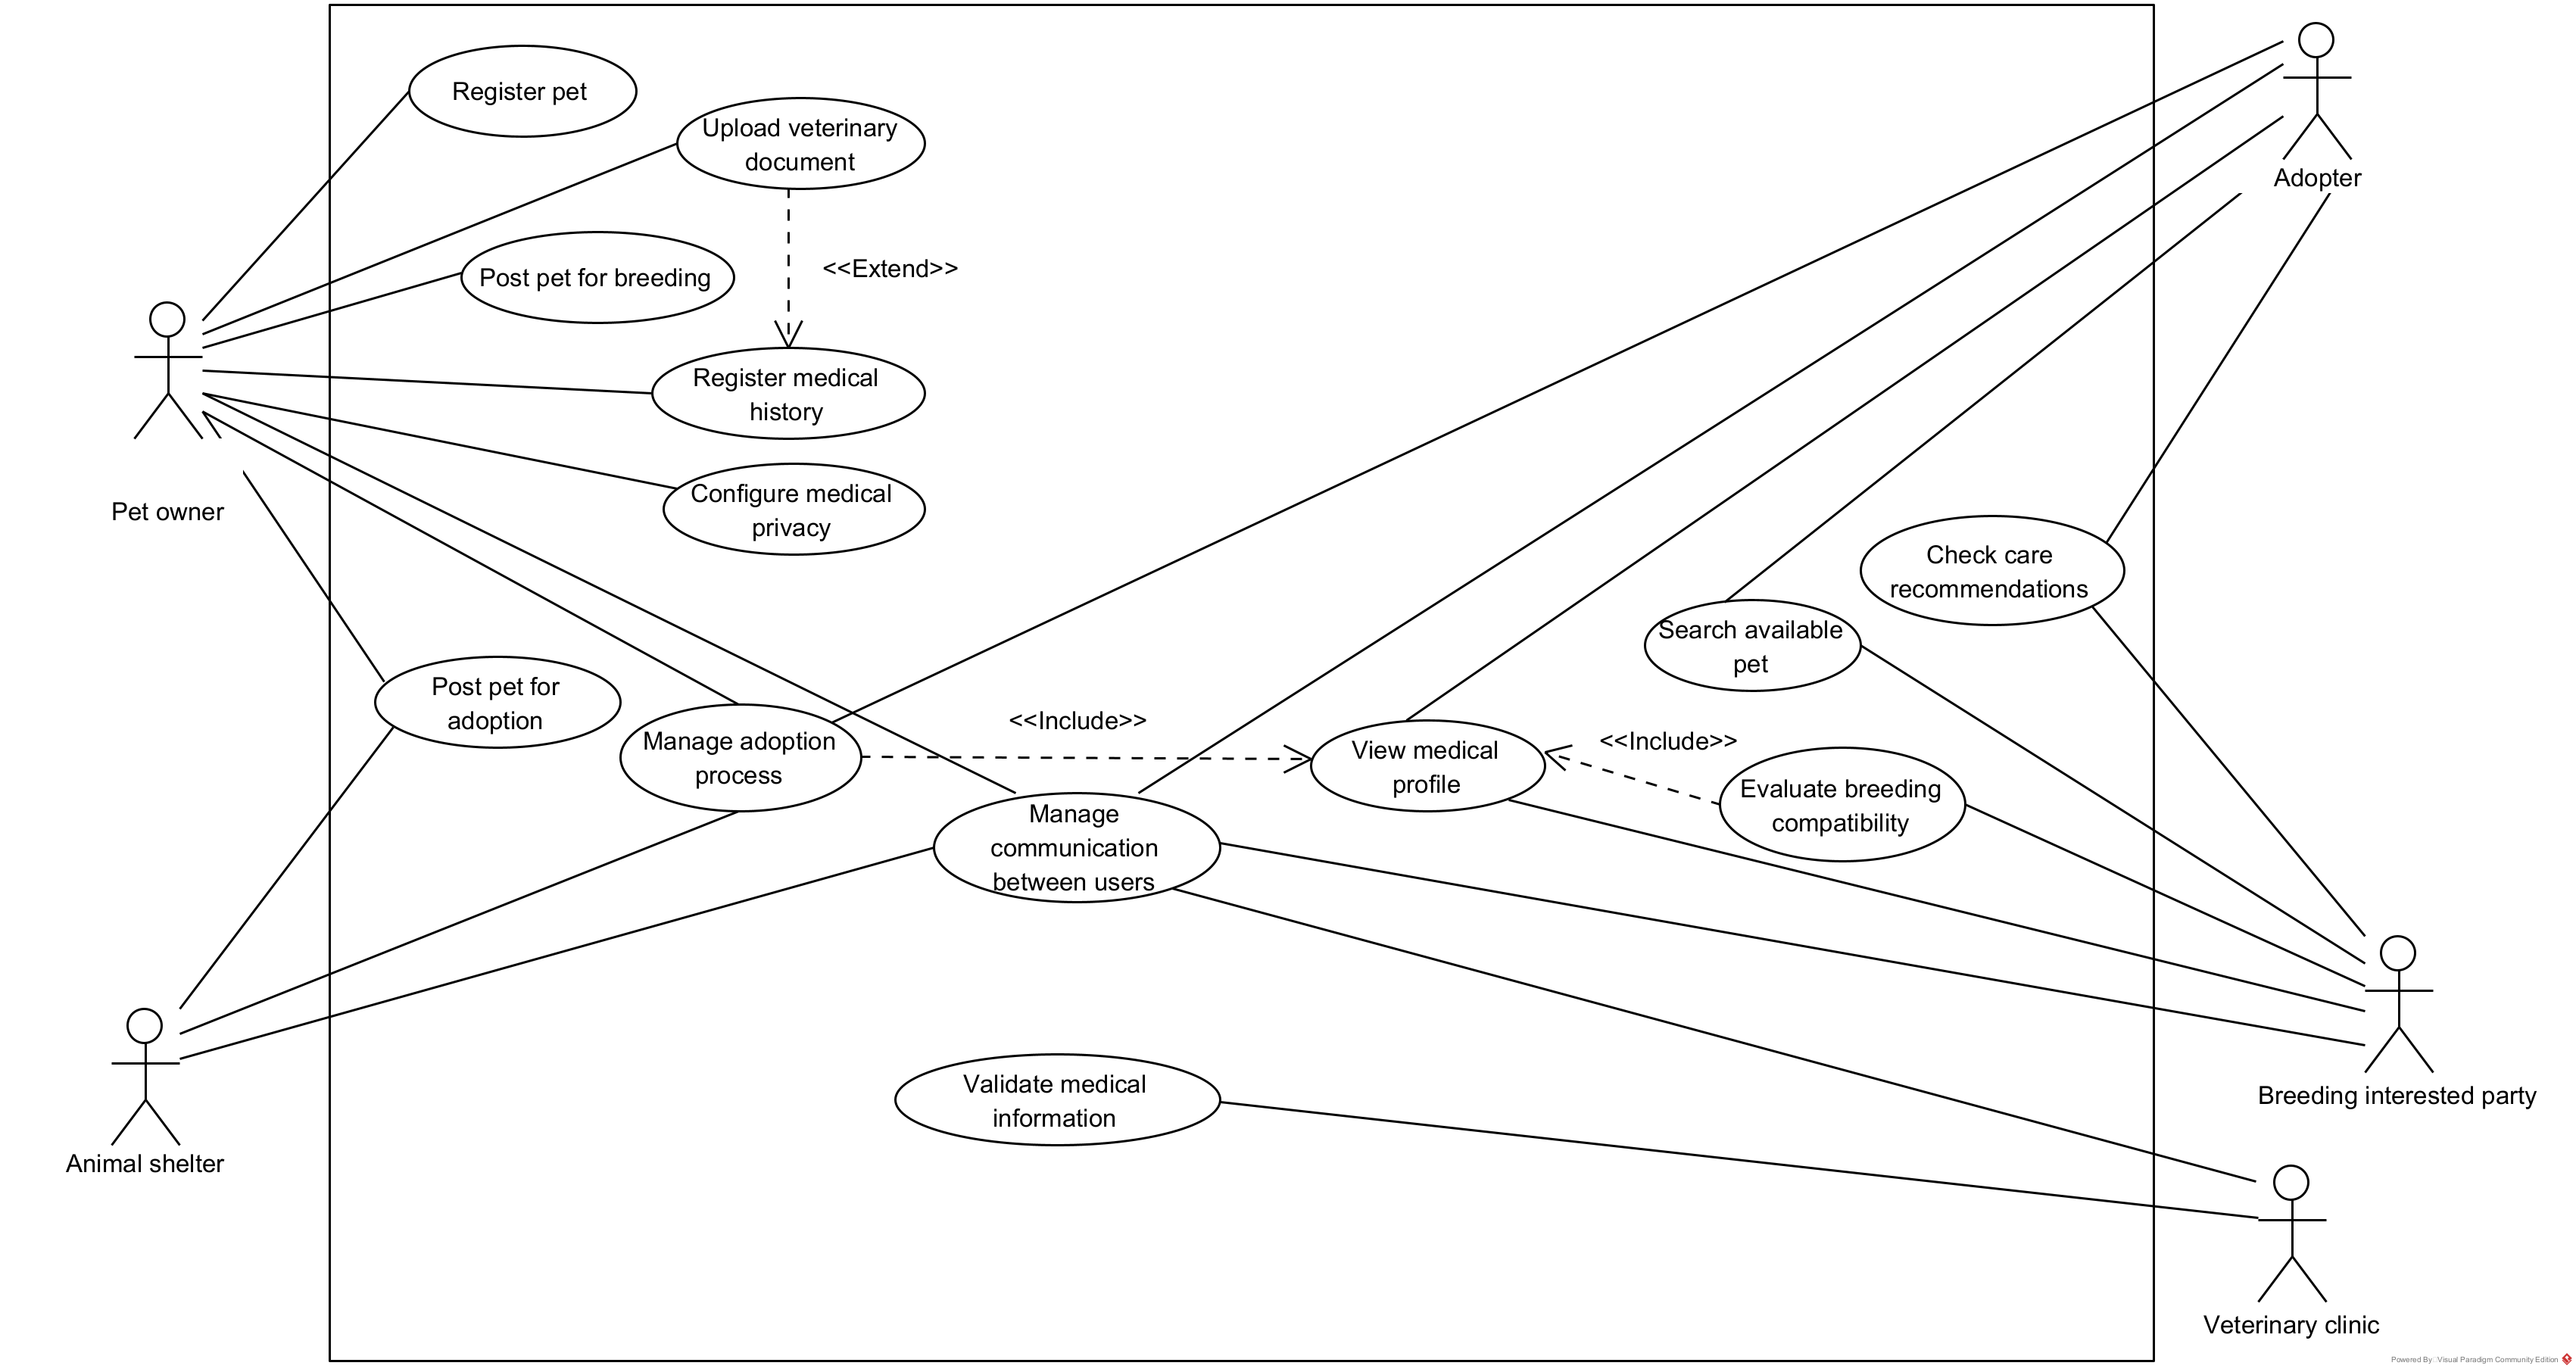
\includegraphics[width=1\textwidth]{figuras/DiagramaCasosDeUso_MundiPets.png}
		\caption{Diagrama de casos de uso general del sistema MundiPets.}
		\label{fig:cu-general}
	\end{figure}

	
	% ------------------------------------------------------------
	\subsection{Especificación textual de casos de uso}
	\label{sec:cu-detallado}
	
	A continuación se especifican textualmente los trece casos de uso derivados
	de los requisitos funcionales de prioridad \emph{Debe tener} (Must) y de
	aquellos requisitos \emph{Debería tener} (Should) que resultan
	indispensables para completar los flujos de adopción y cruza. Cada
	especificación sigue la plantilla de la asignatura y mantiene la
	trazabilidad explícita hacia los requisitos de la
	Sección~\ref{sec:rf}. Los diagramas de secuencia
	(Sección~\ref{sec:secuencia}) y de actividad
	(Sección~\ref{sec:actividad}) se corresponden uno a uno con estos casos de
	uso.
	
	\begin{atributos}{CU-01}{CU-01 --- Registrar mascota.}
		Identificador & CU-01 \\
		Nombre & Registrar mascota \\
		Actor principal & Propietario de mascota \\
		Actores secundarios & Refugio de animales; componente de validación de imágenes \\
		RF asociados & RF-01, RF-17, RF-21 \\
		Precondiciones & El propietario está autenticado y su identidad ha sido verificada (RF-12). \\
		Flujo principal &
		\begin{enumerate}[leftmargin=*, nosep]
			\item El propietario accede al formulario de registro de mascota.
			\item El sistema presenta los campos obligatorios y opcionales.
			\item El propietario ingresa nombre, especie, raza, sexo, edad y estado reproductivo.
			\item El propietario adjunta al menos una fotografía de la mascota.
			\item El sistema valida la completitud de los campos obligatorios.
			\item El sistema envía la fotografía al componente de validación de imágenes (RF-17).
			\item El componente confirma que la imagen corresponde a una mascota y es apropiada.
			\item El sistema almacena el perfil y confirma el registro al propietario.
		\end{enumerate} \\
		Flujos alternativos &
		\begin{enumerate}[leftmargin=*, nosep]
			\item[3.1] El propietario registra el identificador de microchip (RF-21); el sistema lo asocia al perfil.
			\item[8.1] El propietario decide no publicar la mascota; el perfil queda en estado \emph{Registrada}.
		\end{enumerate} \\
		Flujos de excepción &
		\begin{enumerate}[leftmargin=*, nosep]
			\item[5.1] Falta un campo obligatorio: el sistema retorna al formulario señalando el campo incompleto y no invoca la capa de persistencia.
			\item[7.1] La imagen es rechazada por el componente de IA: el sistema notifica el motivo del rechazo (RNF-14) y solicita una nueva fotografía.
		\end{enumerate} \\
		Postcondiciones & El perfil de la mascota queda almacenado en estado \emph{Registrada} y disponible para consulta, publicación y registro de historial médico. \\
	\end{atributos}
	
	\begin{atributos}{CU-02}{CU-02 --- Registrar historial médico y antecedentes genéticos.}
		Identificador & CU-02 \\
		Nombre & Registrar historial médico y antecedentes genéticos \\
		Actor principal & Propietario de mascota \\
		Actores secundarios & Veterinaria \\
		RF asociados & RF-02, RF-16, RF-24 \\
		Precondiciones & La mascota está registrada en el sistema (CU-01) y el usuario tiene permisos de escritura sobre su historial. \\
		Flujo principal &
		\begin{enumerate}[leftmargin=*, nosep]
			\item El usuario selecciona la mascota y accede a su historial médico.
			\item El sistema muestra el historial vigente y el formulario de registro.
			\item El usuario registra vacunas, desparasitaciones, enfermedades, alergias o tratamientos.
			\item El usuario ingresa la trazabilidad de cepa, lote y profesional aplicador de cada vacuna (RF-24).
			\item El usuario registra los antecedentes genéticos y de parentesco de la mascota (RF-16).
			\item El sistema valida el formato y la coherencia temporal de las fechas ingresadas.
			\item El sistema almacena el registro y actualiza el historial médico.
		\end{enumerate} \\
		Flujos alternativos &
		\begin{enumerate}[leftmargin=*, nosep]
			\item[7.1] Si quien registra es una \textbf{veterinaria} autorizada, el sistema marca el registro como validado profesionalmente (RD-03) e identifica al profesional responsable.
			\item[7.2] Si quien registra es el \textbf{propietario}, el registro queda en estado \emph{PendienteDeValidación} hasta que una veterinaria ejecute CU-09.
		\end{enumerate} \\
		Flujos de excepción &
		\begin{enumerate}[leftmargin=*, nosep]
			\item[6.1] La fecha de aplicación es posterior a la fecha actual: el sistema rechaza el registro y solicita corrección.
			\item[6.2] Falta la cepa o el aplicador de una vacuna: el sistema advierte que el registro no podrá ser validado profesionalmente mientras el dato esté ausente.
		\end{enumerate} \\
		Postcondiciones & El historial médico y los antecedentes genéticos quedan actualizados y disponibles para los usuarios autorizados según la configuración de privacidad (RF-11). \\
	\end{atributos}
	
	\begin{atributos}{CU-03}{CU-03 --- Cargar documento veterinario y carnet de vacunación.}
		Identificador & CU-03 \\
		Nombre & Cargar documento veterinario y carnet de vacunación \\
		Actor principal & Propietario de mascota \\
		Actores secundarios & Veterinaria (validación posterior) \\
		RF asociados & RF-14, RF-24 \\
		Precondiciones & La mascota está registrada y el propietario dispone del documento veterinario digitalizado. \\
		Flujo principal &
		\begin{enumerate}[leftmargin=*, nosep]
			\item El propietario accede a la sección de documentos de la mascota.
			\item El propietario adjunta el archivo del certificado o carnet de vacunación.
			\item El sistema valida el formato y el tamaño del archivo.
			\item El sistema extrae los metadatos del documento (tipo y fecha) y almacena el archivo.
			\item El sistema registra el documento en estado \emph{PendienteDeValidación}.
			\item El sistema actualiza el carnet de vacunación de la mascota y confirma la carga.
		\end{enumerate} \\
		Flujos alternativos &
		\begin{enumerate}[leftmargin=*, nosep]
			\item[4.1] Los metadatos no pueden extraerse automáticamente: el sistema solicita al propietario que ingrese manualmente el tipo y la fecha del documento.
			\item[6.1] Ya existe un documento vigente del mismo tipo: el sistema conserva el anterior como versión histórica y marca el nuevo como vigente.
		\end{enumerate} \\
		Flujos de excepción &
		\begin{enumerate}[leftmargin=*, nosep]
			\item[3.1] El formato del archivo no es admitido o excede el tamaño máximo: el sistema rechaza la carga e informa la restricción.
		\end{enumerate} \\
		Postcondiciones & El documento queda almacenado y visible para el propietario, en estado \emph{PendienteDeValidación} hasta la ejecución de CU-09 por parte de una veterinaria autorizada. \\
	\end{atributos}
	
	\begin{atributos}{CU-04}{CU-04 --- Publicar mascota en adopción.}
		Identificador & CU-04 \\
		Nombre & Publicar mascota en adopción \\
		Actor principal & Propietario de mascota \\
		Actores secundarios & Refugio de animales \\
		RF asociados & RF-13, RF-05 \\
		Precondiciones & La mascota está registrada (CU-01) y el propietario es su titular en el sistema. \\
		Flujo principal &
		\begin{enumerate}[leftmargin=*, nosep]
			\item El propietario selecciona una mascota registrada.
			\item El propietario indica el tipo de disponibilidad: adopción.
			\item El sistema verifica la completitud del perfil (fotografías, vacunas, datos generales).
			\item El sistema habilita la confirmación de la publicación.
			\item El propietario confirma la publicación.
			\item El sistema crea la publicación y la incorpora al listado de mascotas disponibles.
		\end{enumerate} \\
		Flujos alternativos &
		\begin{enumerate}[leftmargin=*, nosep]
			\item[1.1] La mascota ya cuenta con una publicación activa: el sistema ofrece actualizar la publicación existente en lugar de crear un duplicado.
			\item[3.1] El perfil está incompleto: el sistema muestra una advertencia preventiva con los campos faltantes, sin bloquear la publicación.
		\end{enumerate} \\
		Flujos de excepción &
		\begin{enumerate}[leftmargin=*, nosep]
			\item[6.1] La mascota se encuentra en estado \emph{EnProcesoDeAdopción} o \emph{Adoptada}: el sistema impide la publicación e informa el estado vigente.
		\end{enumerate} \\
		Postcondiciones & La mascota transita al estado \emph{Publicada} y queda visible en las búsquedas de adopción (CU-11). \\
	\end{atributos}
	
	\begin{atributos}{CU-05}{CU-05 --- Publicar mascota para cruza y gestionar solicitud.}
		Identificador & CU-05 \\
		Nombre & Publicar mascota para cruza y gestionar solicitud \\
		Actor principal & Propietario de mascota \\
		Actores secundarios & Interesado en cruza \\
		RF asociados & RF-08, RF-13, RF-16, RF-19, RF-27 \\
		Precondiciones & La mascota está registrada y cuenta con antecedentes genéticos registrados (RF-16). \\
		Flujo principal &
		\begin{enumerate}[leftmargin=*, nosep]
			\item El propietario selecciona la mascota e indica disponibilidad para cruza.
			\item El sistema verifica que existan antecedentes genéticos y de parentesco registrados.
			\item El sistema verifica la vigencia del certificado veterinario asociado (RF-19).
			\item El sistema publica la mascota en el listado de cruza responsable.
			\item Un interesado en cruza envía una solicitud sobre la publicación.
			\item El sistema verifica la cantidad de procesos de cruza completados por la mascota en los últimos seis meses (RF-27).
			\item El sistema registra la solicitud en estado \emph{Pendiente} y notifica al propietario.
			\item El propietario acepta o rechaza la solicitud.
			\item El sistema actualiza el estado de la solicitud y notifica al interesado.
		\end{enumerate} \\
		Flujos alternativos &
		\begin{enumerate}[leftmargin=*, nosep]
			\item[2.1] No existen antecedentes genéticos: el sistema redirige al propietario al formulario de RF-16 antes de permitir continuar.
			\item[6.1] La mascota supera los dos procesos de cruza completados en seis meses: el sistema muestra la alerta de uso repetitivo (RF-27) al propietario y al interesado antes de continuar, sin bloquear de forma definitiva la solicitud.
			\item[8.1] El propietario acepta: el sistema habilita el canal de comunicación (CU-08) y la mascota transita a \emph{EnProcesoDeCruza}.
		\end{enumerate} \\
		Flujos de excepción &
		\begin{enumerate}[leftmargin=*, nosep]
			\item[3.1] El certificado veterinario está vencido o no validado: el sistema impide la publicación e informa el requisito pendiente.
		\end{enumerate} \\
		Postcondiciones & La publicación de cruza queda activa y las solicitudes recibidas quedan registradas con su estado y fecha para su consulta posterior (CU-07), incluyendo el conteo actualizado de procesos de cruza de la mascota para la alerta de uso repetitivo (RF-27). \\
	\end{atributos}
	
	\begin{atributos}{CU-06}{CU-06 --- Evaluar compatibilidad de cruza.}
		Identificador & CU-06 \\
		Nombre & Evaluar compatibilidad de cruza \\
		Actor principal & Interesado en cruza \\
		Actores secundarios & Propietario de mascota; componente de inteligencia artificial \\
		RF asociados & RF-06, RF-16, RF-23 \\
		Precondiciones & Ambas mascotas están registradas, publicadas para cruza y cuentan con historial médico y antecedentes genéticos. \\
		Flujo principal &
		\begin{enumerate}[leftmargin=*, nosep]
			\item El usuario selecciona las dos mascotas a comparar.
			\item El sistema recupera los datos generales, el historial médico y los antecedentes genéticos de ambas.
			\item El sistema ejecuta la verificación de parentesco (CU-13).
			\item El sistema envía los datos al componente de evaluación de compatibilidad.
			\item El componente calcula el resultado orientativo y genera la explicación causal asociada (RNF-13).
			\item El sistema presenta el resultado junto con los factores que lo sustentan.
			\item El sistema registra la evaluación para su consulta posterior.
		\end{enumerate} \\
		Flujos alternativos &
		\begin{enumerate}[leftmargin=*, nosep]
			\item[3.1] Se detecta un grado de parentesco incompatible: el sistema muestra una alerta explícita (RF-23) y finaliza sin generar recomendación.
			\item[6.1] El resultado indica riesgo sanitario: el sistema adjunta la alerta correspondiente antes de mostrar el resultado.
		\end{enumerate} \\
		Flujos de excepción &
		\begin{enumerate}[leftmargin=*, nosep]
			\item[2.1] Una de las mascotas carece de antecedentes genéticos: el sistema informa que la evaluación no puede realizarse y señala la información faltante.
			\item[5.1] El componente de IA no responde dentro del umbral definido en RNF-03: el sistema informa la indisponibilidad temporal del servicio.
		\end{enumerate} \\
		Postcondiciones & El usuario dispone de un resultado orientativo de compatibilidad con su explicación causal; el resultado no sustituye la valoración profesional veterinaria. \\
	\end{atributos}
	
	\begin{atributos}{CU-07}{CU-07 --- Consultar historial de procesos de adopción y cruza.}
		Identificador & CU-07 \\
		Nombre & Consultar historial de procesos de adopción y cruza \\
		Actor principal & Propietario de mascota \\
		Actores secundarios & Refugio de animales \\
		RF asociados & RF-15, RF-05, RF-08 \\
		Precondiciones & El propietario está autenticado y posee al menos una mascota con solicitudes registradas. \\
		Flujo principal &
		\begin{enumerate}[leftmargin=*, nosep]
			\item El propietario accede a la sección de historial de procesos.
			\item El sistema recupera en paralelo las solicitudes de adopción y de cruza asociadas a sus mascotas.
			\item El sistema combina ambos conjuntos en una línea de tiempo ordenada por fecha.
			\item El sistema determina, para cada solicitud, el nivel de información visible según su estado.
			\item El sistema presenta el historial consolidado con el estado vigente de cada proceso.
		\end{enumerate} \\
		Flujos alternativos &
		\begin{enumerate}[leftmargin=*, nosep]
			\item[5.1] El propietario filtra el historial por mascota, tipo de proceso o rango de fechas.
		\end{enumerate} \\
		Flujos de excepción &
		\begin{enumerate}[leftmargin=*, nosep]
			\item[2.1] No existen solicitudes registradas: el sistema muestra un mensaje informativo en lugar de una lista vacía.
		\end{enumerate} \\
		Postcondiciones & El propietario visualiza la trazabilidad completa de sus procesos sin que se expongan datos de contacto de solicitantes no aceptados, en cumplimiento del principio de minimización de datos (RL-05). \\
	\end{atributos}
	
	\begin{atributos}{CU-08}{CU-08 --- Gestionar comunicación entre usuarios.}
		Identificador & CU-08 \\
		Nombre & Gestionar comunicación entre usuarios \\
		Actor principal & Propietario de mascota, Adoptante, Interesado en cruza \\
		Actores secundarios & Refugio de animales; componente de moderación automática \\
		RF asociados & RF-07 \\
		Precondiciones & Existe una solicitud de adopción o cruza que habilita el canal de comunicación entre ambas partes. \\
		Flujo principal &
		\begin{enumerate}[leftmargin=*, nosep]
			\item El usuario abre la conversación asociada a la solicitud.
			\item El usuario redacta y envía un mensaje.
			\item El sistema envía el contenido al componente de moderación automática.
			\item El componente clasifica el mensaje como apropiado.
			\item El sistema almacena el mensaje y lo entrega al destinatario.
			\item El sistema notifica al destinatario la recepción del mensaje.
		\end{enumerate} \\
		Flujos alternativos &
		\begin{enumerate}[leftmargin=*, nosep]
			\item[2.1] El usuario adjunta una imagen; el sistema la somete a la validación de imágenes (RF-17) antes de la moderación de texto.
		\end{enumerate} \\
		Flujos de excepción &
		\begin{enumerate}[leftmargin=*, nosep]
			\item[4.1] El mensaje es marcado como inapropiado: el sistema bloquea el envío y notifica al remitente la categoría de infracción detectada conforme a RNF-15, sin entregarlo al destinatario.
			\item[5.1] El destinatario ha bloqueado la conversación: el sistema impide el envío e informa al remitente.
		\end{enumerate} \\
		Postcondiciones & Únicamente los mensajes que superan la moderación quedan persistidos y disponibles en el historial de la conversación. \\
	\end{atributos}
	
	\begin{atributos}{CU-09}{CU-09 --- Validar información médica.}
		Identificador & CU-09 \\
		Nombre & Validar información médica \\
		Actor principal & Veterinaria \\
		Actores secundarios & Propietario de mascota \\
		RF asociados & RF-09, RF-14, RF-24, RF-26 \\
		Precondiciones & La veterinaria está autenticada, su identidad profesional ha sido verificada (RF-12) y existe información médica en estado \emph{PendienteDeValidación}. \\
		Flujo principal &
		\begin{enumerate}[leftmargin=*, nosep]
			\item La veterinaria accede a la bandeja de registros pendientes de validación.
			\item La veterinaria selecciona el historial médico o documento a revisar.
			\item El sistema muestra el registro junto con el documento adjunto.
			\item La veterinaria contrasta la información y aprueba el registro.
			\item El sistema marca el registro como \emph{Validado} y asocia la identificación del profesional responsable.
			\item El sistema notifica al propietario el resultado de la validación.
		\end{enumerate} \\
		Flujos alternativos &
		\begin{enumerate}[leftmargin=*, nosep]
			\item[4.1] La veterinaria rechaza el registro: el sistema exige el ingreso de una observación técnica antes de confirmar la operación y el registro transita a \emph{Rechazado}.
			\item[5.1] Una segunda veterinaria autorizada solicita revisar un registro ya validado (RF-26): el sistema le muestra el registro y la validación previa, y permite confirmar o cuestionar el resultado sin sustituir la primera validación.
		\end{enumerate} \\
		Flujos de excepción &
		\begin{enumerate}[leftmargin=*, nosep]
			\item[4.2] La veterinaria intenta rechazar sin observación técnica: el sistema impide confirmar la operación e indica el campo obligatorio.
			\item[3.1] El documento adjunto es ilegible: la veterinaria registra la observación correspondiente y el registro se devuelve al propietario para su reemplazo.
		\end{enumerate} \\
		Postcondiciones & El registro médico queda en estado \emph{Validado} o \emph{Rechazado} con trazabilidad del profesional responsable y de la fecha de la resolución, en cumplimiento de RD-03 y RNF-05, y puede quedar con una segunda validación registrada cuando aplica RF-26. \\
	\end{atributos}
	
	\begin{atributos}{CU-10}{CU-10 --- Consultar perfil médico.}
		Identificador & CU-10 \\
		Nombre & Consultar perfil médico \\
		Actor principal & Adoptante, Interesado en cruza \\
		Actores secundarios & Propietario de mascota, Veterinaria \\
		RF asociados & RF-03, RF-11 \\
		Precondiciones & La mascota existe en el sistema y el usuario consultante está autenticado. \\
		Flujo principal &
		\begin{enumerate}[leftmargin=*, nosep]
			\item El usuario selecciona una mascota desde el resultado de una búsqueda o publicación.
			\item El sistema determina el nivel de acceso del usuario consultante.
			\item El sistema recupera los datos generales, el historial médico y las fotografías de la mascota.
			\item El sistema aplica las reglas de privacidad configuradas por el propietario (RF-11).
			\item El sistema filtra la ubicación exacta y los datos de contacto directo, mostrando únicamente la zona aproximada (RNF-16).
			\item El sistema presenta el perfil resultante al usuario.
		\end{enumerate} \\
		Flujos alternativos &
		\begin{enumerate}[leftmargin=*, nosep]
			\item[2.1] El consultante es el propietario: el sistema muestra el perfil completo sin filtrado.
			\item[2.2] El consultante es una veterinaria autorizada: el sistema muestra los campos médicos obligatorios aun cuando el propietario los haya restringido para otros roles (RD-03).
		\end{enumerate} \\
		Flujos de excepción &
		\begin{enumerate}[leftmargin=*, nosep]
			\item[3.1] La publicación fue retirada o la mascota fue eliminada: el sistema informa que el perfil ya no está disponible.
		\end{enumerate} \\
		Postcondiciones & El usuario obtiene la información autorizada necesaria para tomar una decisión informada sobre adopción o cruza, sin exposición de datos sensibles restringidos. \\
	\end{atributos}
	
	\begin{atributos}{CU-11}{CU-11 --- Buscar mascota disponible.}
		Identificador & CU-11 \\
		Nombre & Buscar mascota disponible \\
		Actor principal & Adoptante, Interesado en cruza \\
		Actores secundarios & --- \\
		RF asociados & RF-04, RF-13 \\
		Precondiciones & Existen publicaciones activas de mascotas en el sistema. \\
		Flujo principal &
		\begin{enumerate}[leftmargin=*, nosep]
			\item El usuario accede al buscador de mascotas.
			\item El usuario selecciona los criterios de filtrado: especie, raza, edad, ubicación aproximada, tamaño, temperamento y tipo de disponibilidad.
			\item El sistema consulta el repositorio de publicaciones activas.
			\item El sistema aplica de forma acumulativa todos los filtros seleccionados.
			\item El sistema ordena los resultados por relevancia o cercanía.
			\item El sistema presenta la lista de mascotas coincidentes.
		\end{enumerate} \\
		Flujos alternativos &
		\begin{enumerate}[leftmargin=*, nosep]
			\item[6.1] El usuario selecciona una mascota del listado e invoca CU-10 para consultar su perfil.
		\end{enumerate} \\
		Flujos de excepción &
		\begin{enumerate}[leftmargin=*, nosep]
			\item[5.1] No existen coincidencias: el sistema informa el resultado vacío y ofrece ajustar o relajar los criterios antes de repetir la búsqueda.
		\end{enumerate} \\
		Postcondiciones & El usuario obtiene un conjunto de publicaciones que cumplen simultáneamente todos los criterios aplicados. \\
	\end{atributos}
	
	\begin{atributos}{CU-12}{CU-12 --- Configurar privacidad médica.}
		Identificador & CU-12 \\
		Nombre & Configurar privacidad médica \\
		Actor principal & Propietario de mascota \\
		Actores secundarios & Veterinaria (destinataria de la excepción de visibilidad) \\
		RF asociados & RF-11, RF-03 \\
		Precondiciones & El propietario está autenticado y posee al menos una mascota registrada. \\
		Flujo principal &
		\begin{enumerate}[leftmargin=*, nosep]
			\item El propietario accede a la configuración de privacidad de la mascota.
			\item El sistema muestra las categorías de datos sensibles: ubicación, contacto y afecciones específicas.
			\item El propietario define el nivel de visibilidad para cada categoría y rol.
			\item El sistema verifica si alguno de los campos restringidos es obligatorio para la validación veterinaria.
			\item El sistema guarda la configuración y confirma la operación.
			\item El sistema aplica las nuevas reglas a todas las consultas posteriores (CU-10).
		\end{enumerate} \\
		Flujos alternativos &
		\begin{enumerate}[leftmargin=*, nosep]
			\item[4.1] Un campo médico obligatorio ha sido restringido: el sistema muestra una advertencia, conserva ese campo visible para las veterinarias autorizadas y guarda el resto de la configuración con normalidad.
		\end{enumerate} \\
		Flujos de excepción &
		\begin{enumerate}[leftmargin=*, nosep]
			\item[5.1] La configuración no puede almacenarse: el sistema conserva la configuración anterior e informa el error, evitando estados de privacidad indeterminados.
		\end{enumerate} \\
		Postcondiciones & La configuración de privacidad queda vigente y se aplica de forma inmediata sobre todas las consultas del perfil, garantizando la visibilidad mínima exigida por RD-03. \\
	\end{atributos}
	
	\begin{atributos}{CU-13}{CU-13 --- Verificación de parentesco previa a la evaluación de compatibilidad.}
		Identificador & CU-13 \\
		Nombre & Evaluar compatibilidad de cruza --- verificación de parentesco \\
		Actor principal & Interesado en cruza \\
		Actores secundarios & Propietario de mascota; componente de inteligencia artificial \\
		RF asociados & RF-06, RF-16, RF-23 \\
		Precondiciones & Ambas mascotas cuentan con antecedentes genéticos y de linaje registrados (RF-16). \\
		Flujo principal &
		\begin{enumerate}[leftmargin=*, nosep]
			\item El sistema recibe la solicitud de evaluación con las dos mascotas seleccionadas.
			\item El sistema recupera el linaje declarado de ambas mascotas.
			\item El sistema ejecuta una comprobación determinística del grado de parentesco.
			\item El sistema determina que no existe incompatibilidad por parentesco.
			\item El sistema habilita la invocación del componente de evaluación de compatibilidad (CU-06).
		\end{enumerate} \\
		Flujos alternativos &
		\begin{enumerate}[leftmargin=*, nosep]
			\item[3.1] Se detecta un grado de parentesco incompatible: el flujo se dirige a la actividad de alerta explícita, se notifica al usuario y se finaliza sin invocar el componente de IA ni generar recomendación alguna.
		\end{enumerate} \\
		Flujos de excepción &
		\begin{enumerate}[leftmargin=*, nosep]
			\item[2.1] El linaje de alguna de las mascotas es desconocido o está incompleto: el sistema advierte que la verificación no es concluyente y deja constancia de la limitación junto al resultado.
		\end{enumerate} \\
		Postcondiciones & La evaluación de compatibilidad solo se ejecuta sobre parejas sin incompatibilidad de parentesco, optimizando el uso del componente de IA y evitando recomendaciones inviables por regla de negocio. \\
	\end{atributos}
	
	% ------------------------------------------------------------
	\subsection{Diagrama de clases refinado}
	\label{sec:clases-refinado}

	El diagrama de clases refinado profundiza el modelo conceptual presentado en
	la Entrega 2 (1B), incorporando los atributos, tipos de dato,
	multiplicidades y operaciones necesarios para representar con precisión las
	27 funcionalidades definidas en la Sección~\ref{sec:rf}. Los nombres de
	clases, atributos y métodos se mantienen en inglés, tal como fueron
	modelados en la herramienta UML, para evitar una traducción que introduzca
	inconsistencias entre el diagrama y el código fuente que lo implementa.

	El modelo se organiza alrededor de la clase \texttt{Pet}, que concentra
	los datos generales exigidos por RF-01 (\texttt{breed}, \texttt{name},
	\texttt{species}, \texttt{petPhotos}, \texttt{birthDate}) y se asocia
	mediante composición (rombo relleno) con \texttt{MedicalHistory}, que
	incorpora el antecedente genético exigido por RF-16 como su atributo
	\texttt{geneticBackground} en lugar de una clase separada. \texttt{Pet} se
	relaciona además con \texttt{PetVaccine} (RF-14), una clase asociativa que
	enlaza cada aplicación de vacuna con su \texttt{Pet} y su
	\texttt{Vaccine}; con \texttt{VetDocument} (RF-19), que registra el estado
	de revisión de cada certificado adjunto; con \texttt{PrivacySettings}
	(RF-11), que administra la visibilidad de la ubicación y el contacto; y
	con \texttt{Interaction} (RF-20, RF-23), que registra los encuentros entre
	dos mascotas y su estado de riesgo.

	Las clases \texttt{Owner}, \texttt{Shelter} y \texttt{Veterinarian} se
	modelan mediante una jerarquía de generalización a partir de
	\texttt{User}, que centraliza los atributos comunes de autenticación y
	verificación de identidad (RF-12) y evita duplicar reglas de acceso entre
	los distintos roles descritos en RD-02; \texttt{User} envía y recibe
	instancias de \texttt{Message} (RF-07) y presenta la operación
	\texttt{verifyIdentity()} exigida por RF-12. La clase
	\texttt{AdoptionRequest} incorpora los atributos de justificación y
	condiciones del hogar exigidos por RF-05, mientras que
	\texttt{BreedingRequest} se asocia con \texttt{CompatibilityEvaluation}
	para representar el resultado orientativo generado por el componente de
	inteligencia artificial (RF-06); ninguna de las dos clases de solicitud
	incorpora de forma explícita las etapas de entrevista, visita y periodo de
	prueba exigidas por RF-18, que se representan en cambio en la máquina de
	estados de \texttt{AdoptionRequest} (Sección~\ref{sec:estados}) y no como
	atributos del diagrama de clases.

	La clase \texttt{Post} centraliza la publicación de disponibilidad
	exigida por RF-13, y \texttt{VeterinaryEvaluation} registra la validación
	profesional exigida por RF-09, con las operaciones
	\texttt{validateHistory()} y \texttt{registerEvaluation()} de
	\texttt{Veterinarian} como su contraparte de comportamiento. Las
	multiplicidades reflejan las reglas de negocio ya validadas en el ERS: un
	\texttt{Pet} puede tener múltiples registros de \texttt{MedicalHistory} y
	de \texttt{PetVaccine} pero pertenece a un único \texttt{Owner}
	(asociación \emph{owns}); una \texttt{BreedingRequest} involucra dos
	mascotas distintas mediante los atributos \texttt{sourcePetId} y
	\texttt{targetPetId}; y un \texttt{Veterinarian} revisa cero o varios
	\texttt{VetDocument} y realiza cero o varias \texttt{VeterinaryEvaluation}.
	Este nivel de detalle permite que el diagrama sirva como referencia
	directa para el diseño del modelo de datos en la fase de implementación.

	Los dos requisitos funcionales agregados en la revisión 4.0 se apoyan
	íntegramente en las clases ya representadas en el diagrama: RF-26
	reutiliza \texttt{MedicalHistory} y la generalización de
	\texttt{Veterinarian}, registrando la segunda validación como una nueva
	instancia de \texttt{VeterinaryEvaluation}; y RF-27 reutiliza
	\texttt{BreedingRequest}, cuyo atributo \texttt{status} --- ya
	representado en el diagrama --- permite derivar el conteo de procesos en
	estado \emph{Approved} sin necesidad de una clase o un atributo visible
	adicional.

	\paragraph{Corrección de modelado incorporada en esta revisión (4.1).}
	La verificación de esta matriz de trazabilidad contra el diagrama
	(Apéndice~\ref{ap:trazabilidad}, nota posterior a la
	Tabla~\ref{tab:matriz_trazabilidad_completa}) había detectado que tres
	requisitos funcionales no estaban completamente cubiertos por el modelo de
	clases vigente. Las tres correcciones ya fueron incorporadas por el equipo
	de modelado: los atributos \texttt{-microchipId~:~string} y
	\texttt{-microchipDate~:~datetime} en \texttt{Pet} (RF-21); los atributos
	\texttt{-batchNumber~:~string} y \texttt{-administeredBy~:~string} en
	\texttt{PetVaccine} (RF-24); y la clase nueva \texttt{LostPetAlert}
	(RF-25), con los atributos \texttt{-alertId~:~long},
	\texttt{-petId~:~long}, \texttt{-lastSeenLocation~:~string},
	\texttt{-lastSeenDate~:~datetime}, \texttt{-contactPhone~:~string} y
	\texttt{-status~:~string}, y los métodos \texttt{+publishAlert()} y
	\texttt{+resolveAlert()}, en composición 1 a 0..* con \texttt{Pet} y en
	asociación 1 a 0..* con \texttt{Owner} (véase el detalle en el
	Apéndice~\ref{ap:trazabilidad}). La Figura~\ref{fig:clases-refinado}
	--- exportada como vista general del diagrama --- es aún la versión previa
	a esta corrección y no muestra los tres cambios; sí se reflejan, en
	cambio, en la vista parcial \emph{Pets and Health} de la
	Figura~\ref{fig:clases-pets-health}, exportada con posterioridad. Se
	recomienda reemplazar la Figura~\ref{fig:clases-refinado} por una versión
	general actualizada para que ambas vistas sean consistentes entre sí.

	\begin{figure}[H]
		\centering
		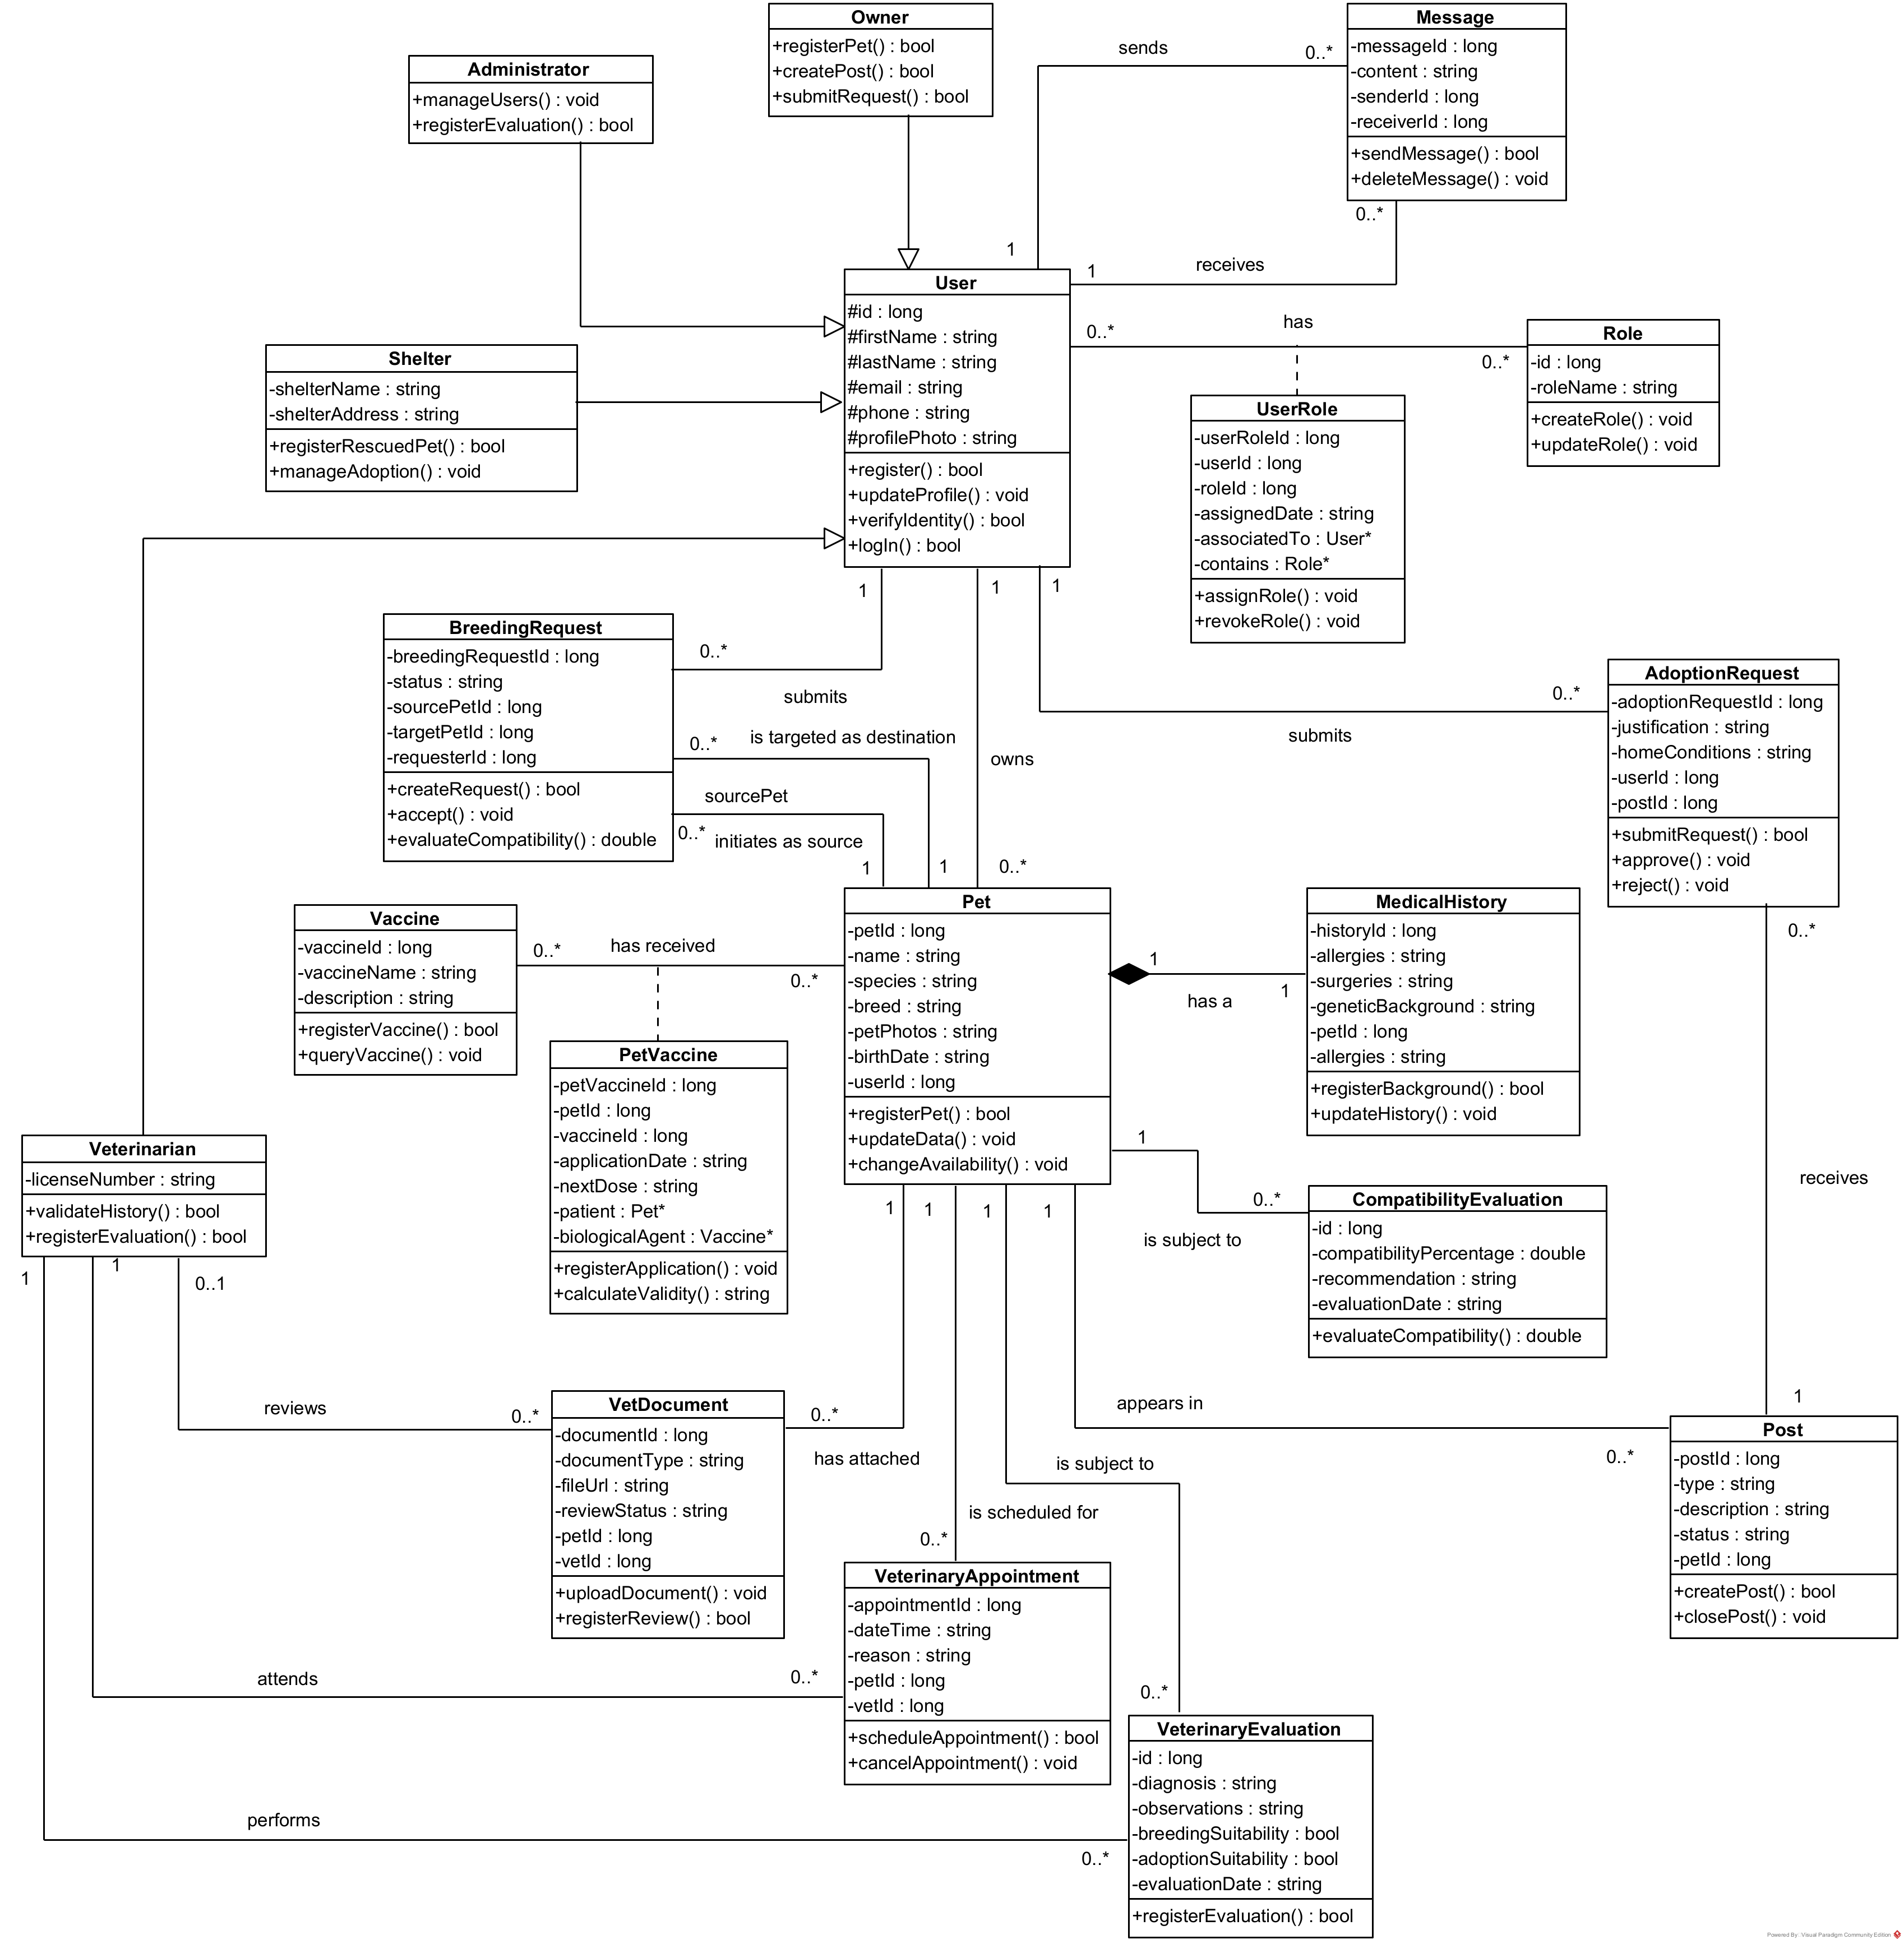
\includegraphics[width=0.72\textwidth]{figuras/DiagramaClasesRefinado_MundiPets.png}
		\caption{Diagrama de clases refinado del sistema MundiPets (vista general, previa a la corrección de modelado de RF-21, RF-24 y RF-25).}
		\label{fig:clases-refinado}
	\end{figure}

	\paragraph{Vistas parciales del diagrama de clases.}
	Para facilitar su lectura, el diagrama de clases refinado se exporta
	también en cuatro vistas parciales correspondientes a los cuatro paquetes
	en los que se organiza: \emph{Users and Roles}, \emph{Applications and
	Evaluations}, \emph{Communication and Publications} y \emph{Pets and
	Health}. Las cuatro vistas son recortes del mismo modelo de la
	Figura~\ref{fig:clases-refinado} y no introducen clases ni atributos
	adicionales, salvo la vista \emph{Pets and Health}, que --- al haberse
	exportado con posterioridad --- sí incorpora ya la corrección de modelado
	de RF-21, RF-24 y RF-25 descrita anteriormente.

	\subsubsection{Users and Roles}

	Esta vista agrupa la jerarquía de usuarios del sistema: \texttt{User} como
	superclase, con los atributos de autenticación comunes (\texttt{id},
	\texttt{firstName}, \texttt{lastName}, \texttt{email}, \texttt{phone},
	\texttt{profilePhoto}) y las operaciones \texttt{register()},
	\texttt{updateProfile()}, \texttt{verifyIdentity()} y \texttt{login()}; y
	sus tres especializaciones por generalización, \texttt{Owner}
	(\texttt{registerPet()}, \texttt{createPost()}, \texttt{submitRequest()}),
	\texttt{Shelter} (\texttt{shelterAddress}; \texttt{registerRescuedPet()},
	\texttt{manageAdoption()}) y \texttt{Veterinarian}
	(\texttt{licenseNumber}; \texttt{validateHistory()},
	\texttt{registerEvaluation()}). La multiplicidad \texttt{0..1} junto a
	\texttt{Veterinarian} refleja que la validación de un registro es
	realizada por, a lo sumo, una veterinaria a la vez, mientras que el
	\texttt{1} junto a \texttt{User} en las asociaciones \emph{sends},
	\emph{receives} y \emph{submits} indica que cada mensaje o solicitud tiene
	exactamente un usuario emisor.

	\begin{figure}[H]
		\centering
		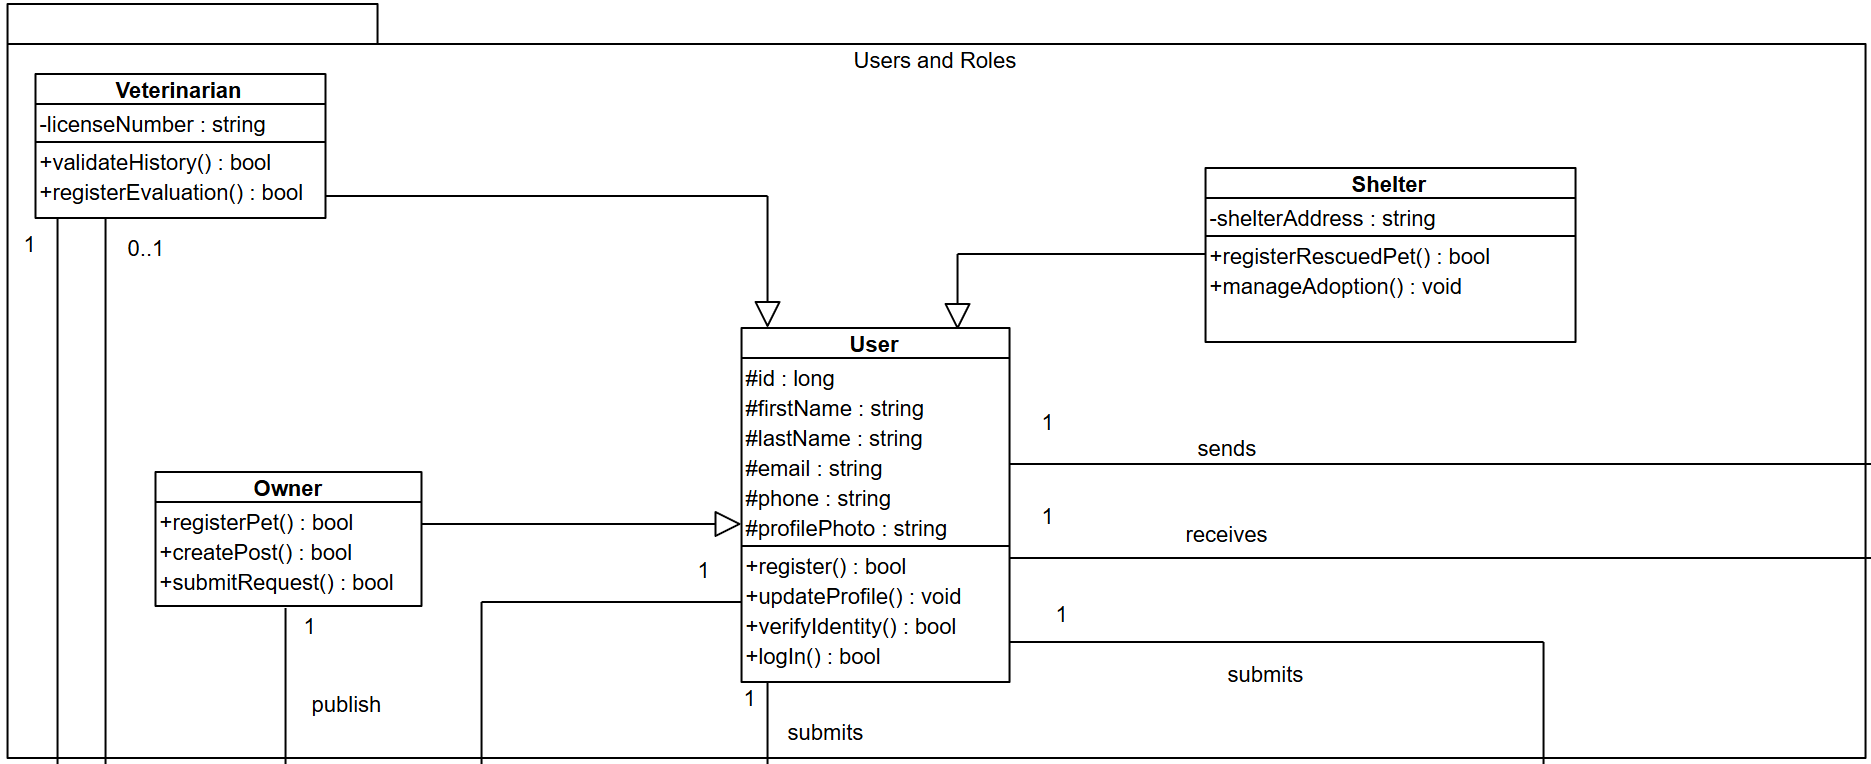
\includegraphics[width=0.95\textwidth]{figuras/DiagramaClasesRefinado_MundiPets_UsersRoles.png}
		\caption{Diagrama de clases refinado --- vista parcial \emph{Users and Roles}.}
		\label{fig:clases-users-roles}
	\end{figure}

	\subsubsection{Applications and Evaluations}

	Esta vista agrupa las tres clases de transacción sobre las que se apoyan
	los procesos de adopción y cruza: \texttt{AdoptionRequest}
	(\texttt{justification}, \texttt{homeConditions}, \texttt{userId},
	\texttt{postId}; \texttt{submitRequest()}, \texttt{approve()},
	\texttt{reject()}), \texttt{BreedingRequest} (\texttt{sourcePetId},
	\texttt{targetPetId}, \texttt{requesterId}; \texttt{createRequest()},
	\texttt{accept()}, \texttt{evaluateCompatibility()},
	\texttt{checkRiskAlert()}) y \texttt{CompatibilityEvaluation}
	(\texttt{compatibilityPercentage}, \texttt{recommendation},
	\texttt{evaluationDate}; \texttt{evaluateCompatibility()}). La relación
	\emph{is subject to} (0..*) entre \texttt{BreedingRequest} y
	\texttt{CompatibilityEvaluation} formaliza que una solicitud de cruza
	puede someterse a más de una evaluación de compatibilidad a lo largo del
	tiempo, mientras que las relaciones \emph{sourcePet} e \emph{is targeted
	as destination}, ambas 0..*, reflejan que una misma mascota puede
	participar como origen o como destino en múltiples solicitudes de cruza
	distintas.

	\begin{figure}[H]
		\centering
		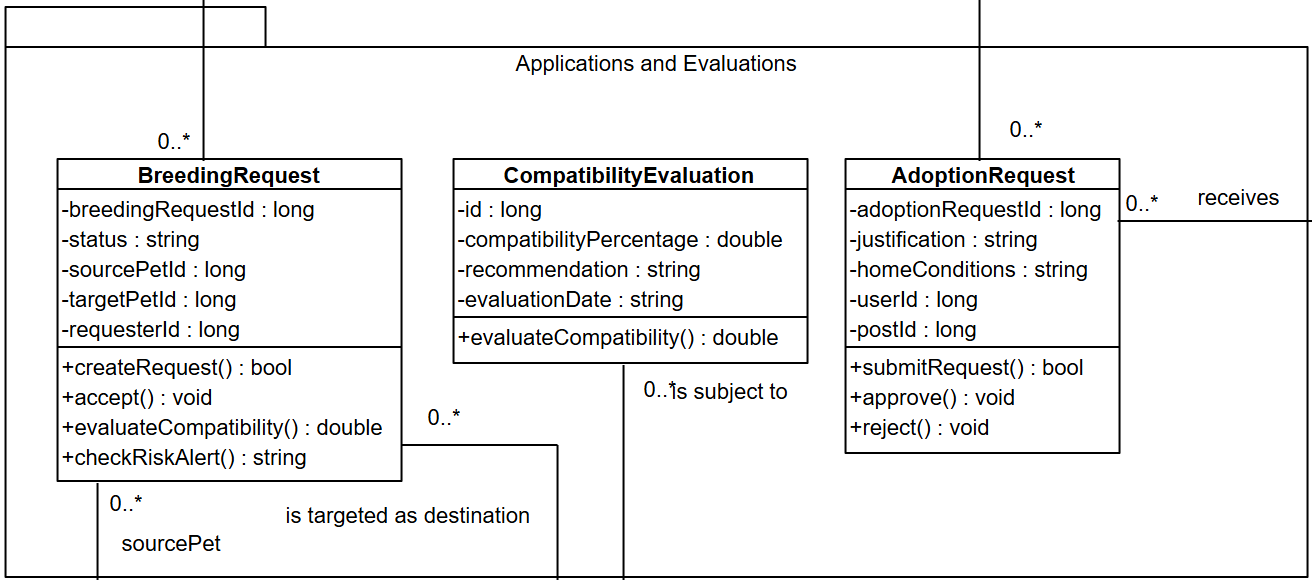
\includegraphics[width=0.95\textwidth]{figuras/DiagramaClasesRefinado_MundiPets_Applications.png}
		\caption{Diagrama de clases refinado --- vista parcial \emph{Applications and Evaluations}.}
		\label{fig:clases-applications}
	\end{figure}

	\subsubsection{Communication and Publications}

	Esta vista, la más reducida de las cuatro, agrupa las dos clases que
	sostienen RF-07 y RF-13: \texttt{Message} (\texttt{messageId},
	\texttt{content}, \texttt{senderId}, \texttt{receiverId};
	\texttt{sendMessage()}, \texttt{deleteMessage()}), asociada 0..* a 0..*
	con \texttt{User} a través de \emph{sends} y \emph{receives}; y
	\texttt{Post} (\texttt{postId}, \texttt{type}, \texttt{description},
	\texttt{status}, \texttt{petId}; \texttt{createPost()},
	\texttt{closePost()}), asociada 1 a 0..* con \texttt{AdoptionRequest} a
	través de \emph{receives}, reflejando que una publicación puede recibir
	cero o varias solicitudes de adopción.

	\begin{figure}[H]
		\centering
		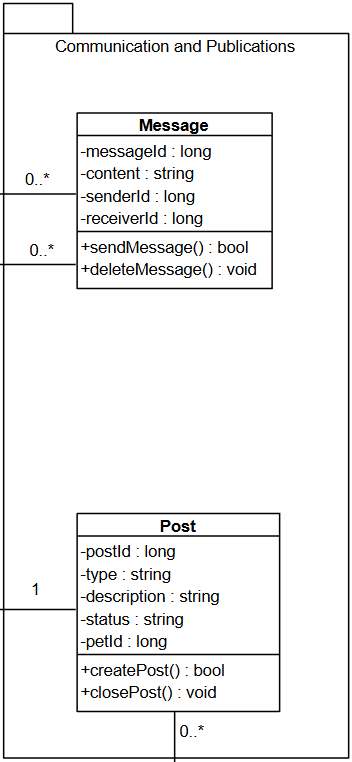
\includegraphics[width=0.55\textwidth]{figuras/DiagramaClasesRefinado_MundiPets_CommunicationPublications.png}
		\caption{Diagrama de clases refinado --- vista parcial \emph{Communication and Publications}.}
		\label{fig:clases-communication}
	\end{figure}

	\subsubsection{Pets and Health}

	Esta es la vista más extensa y concentra la clase central del sistema,
	\texttt{Pet} (\texttt{petId}, \texttt{breed}, \texttt{name},
	\texttt{species}, \texttt{petPhotos}, \texttt{birthDate}, \texttt{userId},
	y --- ya incorporados --- \texttt{microchipId} y \texttt{microchipDate};
	\texttt{registerPet()}, \texttt{updateData()}, \texttt{changeAvailability()}), junto con sus seis asociaciones directas: composición 1 a
	0..* con \texttt{MedicalHistory} (\emph{has a}), asociación 0..* a 0..*
	con \texttt{Vaccine} a través de \texttt{PetVaccine} (\emph{has
	received} --- clase asociativa que ya incorpora \texttt{batchNumber} y
	\texttt{administeredBy}), asociación 1 a 0..* con \texttt{VetDocument}
	(\emph{has attached}), asociación 1 a 1 con \texttt{PrivacySettings}
	(\emph{has a}), asociación 1 a 0..* con \texttt{Interaction}
	(\emph{participe in}) y composición 1 a 0..* con la clase nueva
	\texttt{LostPetAlert} (\emph{warning}). Las clases
	\texttt{VeterinaryEvaluation} (\emph{performs}, 0..* desde
	\texttt{Veterinarian}) e \texttt{Interaction} sustentan respectivamente
	RF-09/RF-26 y RF-20/RF-23, esta última mediante su método
	\texttt{checkRiskAlert()}.

	\begin{figure}[H]
		\centering
		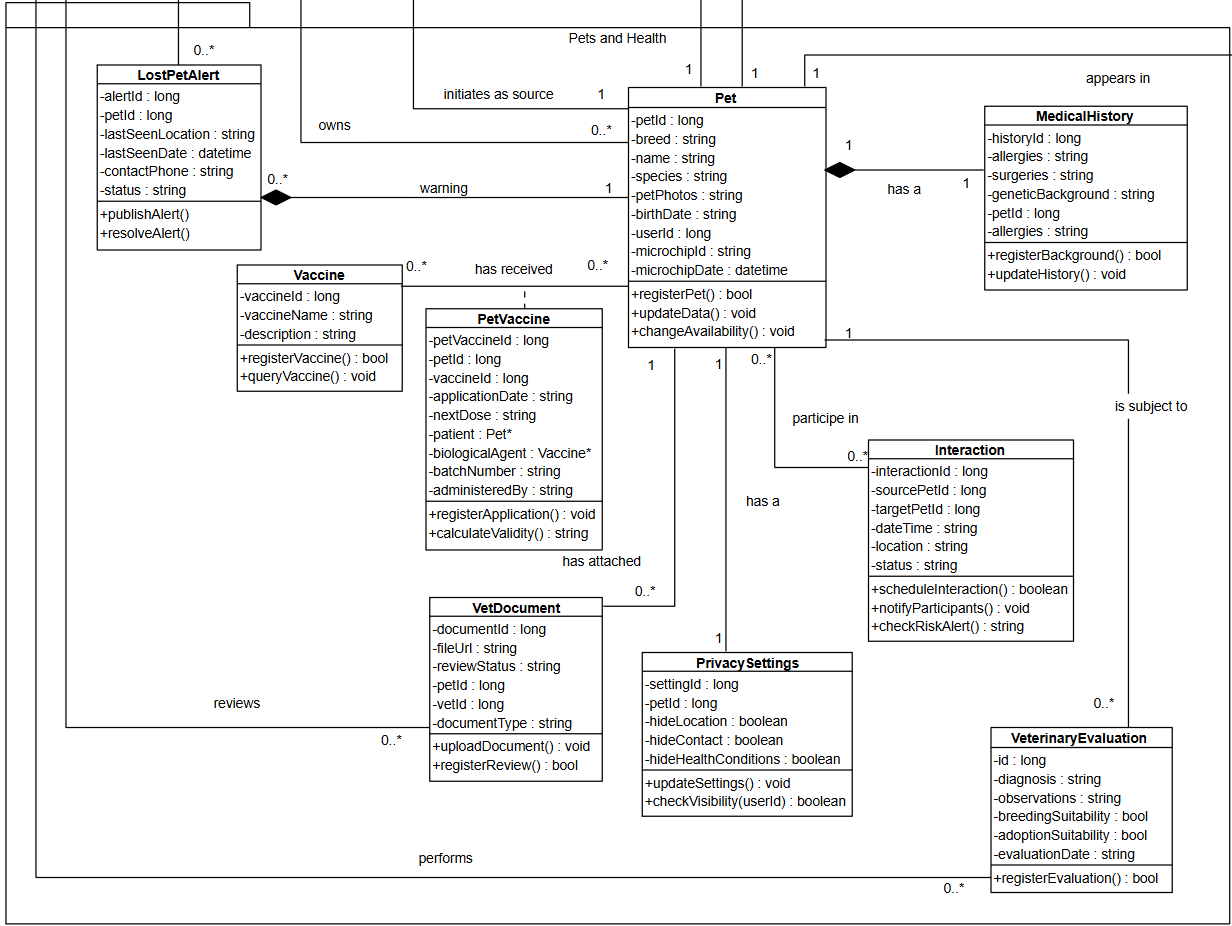
\includegraphics[width=0.95\textwidth]{figuras/DiagramaClasesRefinado_MundiPets_PetsHealth.png}
		\caption{Diagrama de clases refinado --- vista parcial \emph{Pets and Health}, ya con la corrección de modelado de RF-21, RF-24 y RF-25 incorporada.}
		\label{fig:clases-pets-health}
	\end{figure}

	% ------------------------------------------------------------
	\subsection{Diagramas de secuencia}
	\label{sec:secuencia}

	Los diagramas de secuencia detallan la interacción temporal entre los
	actores y los objetos del sistema para los trece casos de uso especificados
	textualmente en la Sección~\ref{sec:cu-detallado}, mostrando el orden de los
	mensajes intercambiados entre el actor, la interfaz, el controlador y los
	objetos de dominio involucrados en cada operación. A continuación se
	presentan los trece diagramas completos (CU-01 a CU-13).

	\paragraph{Nota de verificación (revisión 4.1).} Al contrastar cada figura
	contra la especificación textual de su caso de uso se detectó que los
	archivos de cuatro diagramas no corresponden al caso de uso que su nombre
	de archivo indica: el archivo \texttt{DiagramaSecuencia\_CU-06} contiene en
	realidad la configuración de privacidad médica (CU-12); el archivo
	\texttt{DiagramaSecuencia\_CU-07} contiene la gestión de aceptación o
	rechazo de una solicitud de adopción, sin corresponder de forma exacta a
	ningún CU numerado de la especificación textual vigente; el archivo
	\texttt{DiagramaSecuencia\_CU-12} contiene la consulta de recomendaciones
	de cuidado (relacionada con RF-10), tampoco numerada de forma exacta en la
	especificación textual; y el archivo \texttt{DiagramaSecuencia\_CU-13}
	contiene la evaluación de compatibilidad de cruza (CU-06), integrando en
	un solo diagrama la verificación de parentesco que la especificación
	textual trata por separado como CU-13. Las cuatro descripciones siguientes
	documentan el contenido \textbf{real} de cada archivo tal como fue
	exportado, y se recomienda al equipo renombrar los archivos --- o
	renumerar las subsecciones CU-06, CU-07, CU-12 y CU-13 de la
	Sección~\ref{sec:cu-detallado} --- antes de la entrega final, para que el
	nombre de archivo, el título de la subsección y el contenido de la figura
	coincidan entre sí.

	\subsubsection{Registrar mascota (CU-01)}

	El diagrama de secuencia de CU-01 ilustra el flujo mediante el cual el
	propietario, ya autenticado, selecciona \emph{Register pet}, adjunta entre
	una y cinco fotografías en un ciclo (\emph{loop}) y envía el formulario. El
	controlador (\texttt{PetController}) valida los campos obligatorios
	definidos en RF-01 antes de invocar al repositorio; si la validación falla,
	retorna un mensaje de error específico del campo sin invocar la capa de
	persistencia, evitando así el registro de perfiles incompletos, y si es
	exitosa, confirma el registro al propietario.

	\begin{figure}[H]
		\centering
		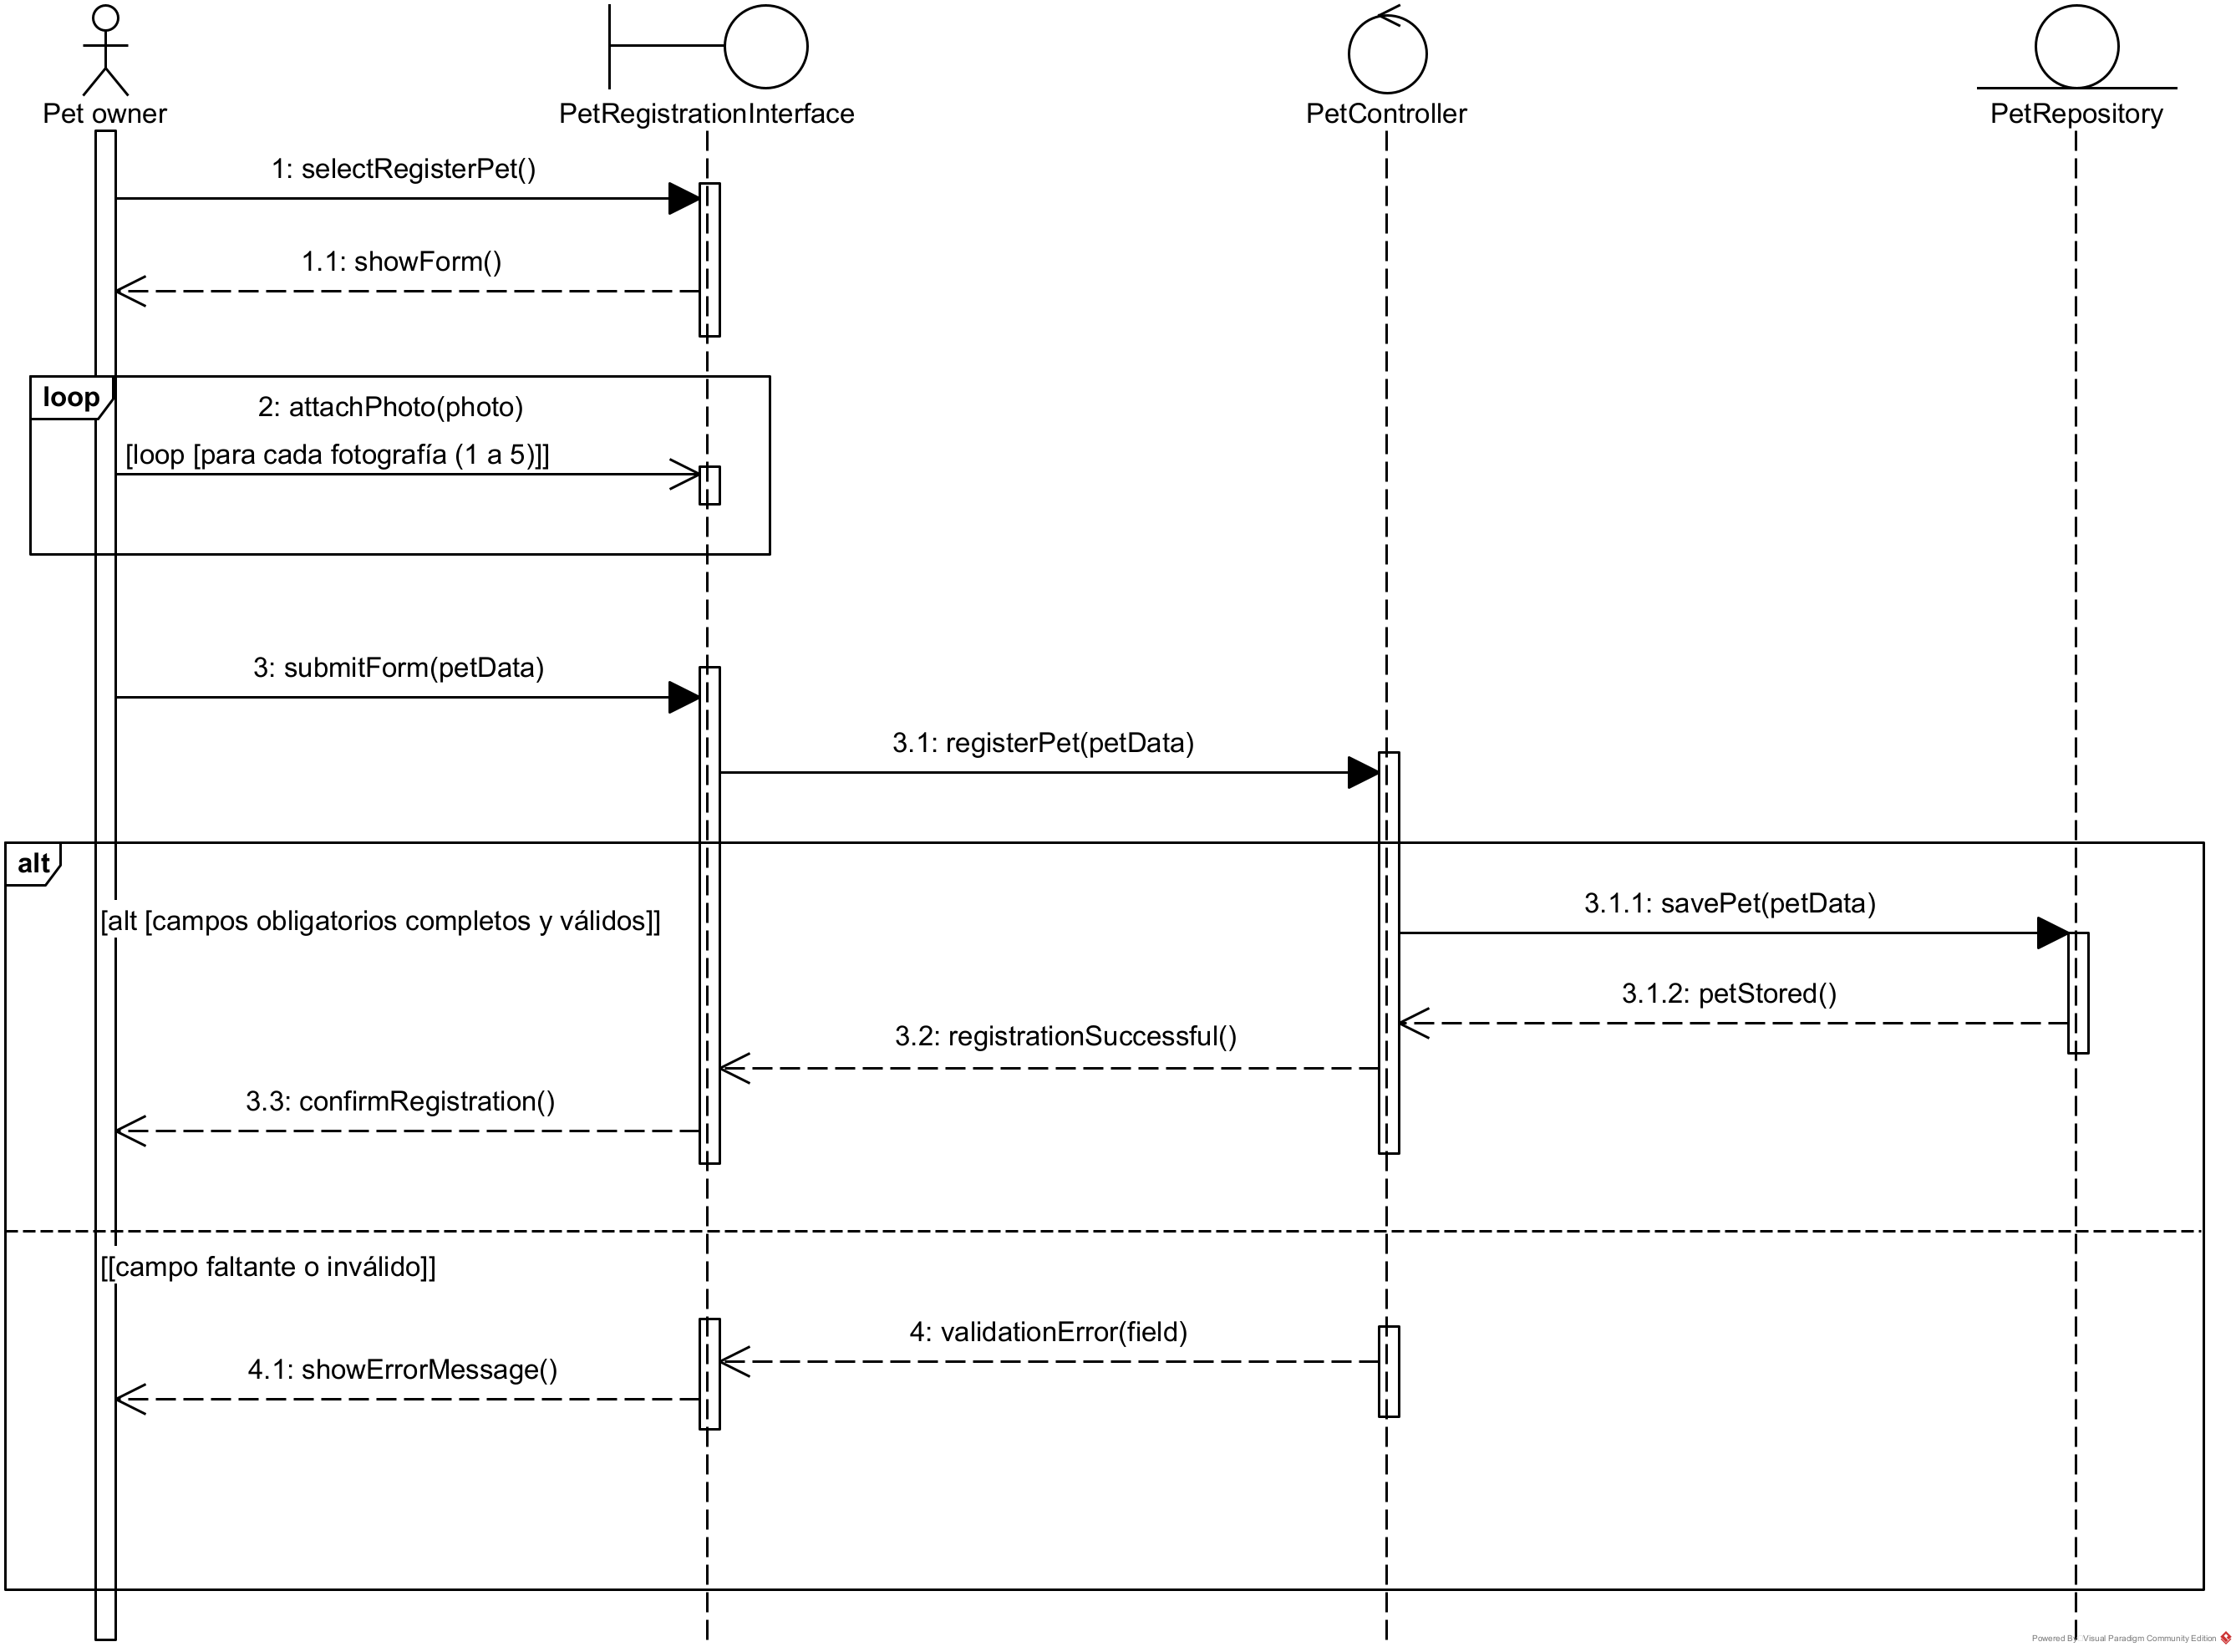
\includegraphics[width=0.72\textwidth]{figuras/DiagramaSecuencia_CU-01_MundiPets.png}
		\caption{Diagrama de secuencia del caso de uso CU-01 --- Registrar mascota.}
		\label{fig:sec-cu01}
	\end{figure}

	\subsubsection{Registrar historial médico y antecedentes genéticos (CU-02)}

	Este diagrama modela la interacción entre el propietario y el sistema al
	registrar la información médica de la mascota (RF-02). El propietario
	completa el formulario (\texttt{fillMedicalData}) y lo envía; el
	controlador (\texttt{MedicalHistoryController}) valida su completitud y lo
	persiste en el repositorio antes de confirmar el registro, o retorna un
	mensaje de error específico si algún campo obligatorio falta o es
	inválido. El diagrama no distingue de forma explícita entre propietario y
	veterinaria como emisores del registro; esa bifurcación de actor, junto
	con la trazabilidad de cepa, lote y aplicador exigida por RF-24, se
	gestiona en el diagrama de estados de verificación de documentos médicos
	(Sección~\ref{sec:estados}) y en el propio modelo de clases
	(\texttt{PetVaccine}), no como una rama adicional de esta secuencia.

	\begin{figure}[H]
		\centering
		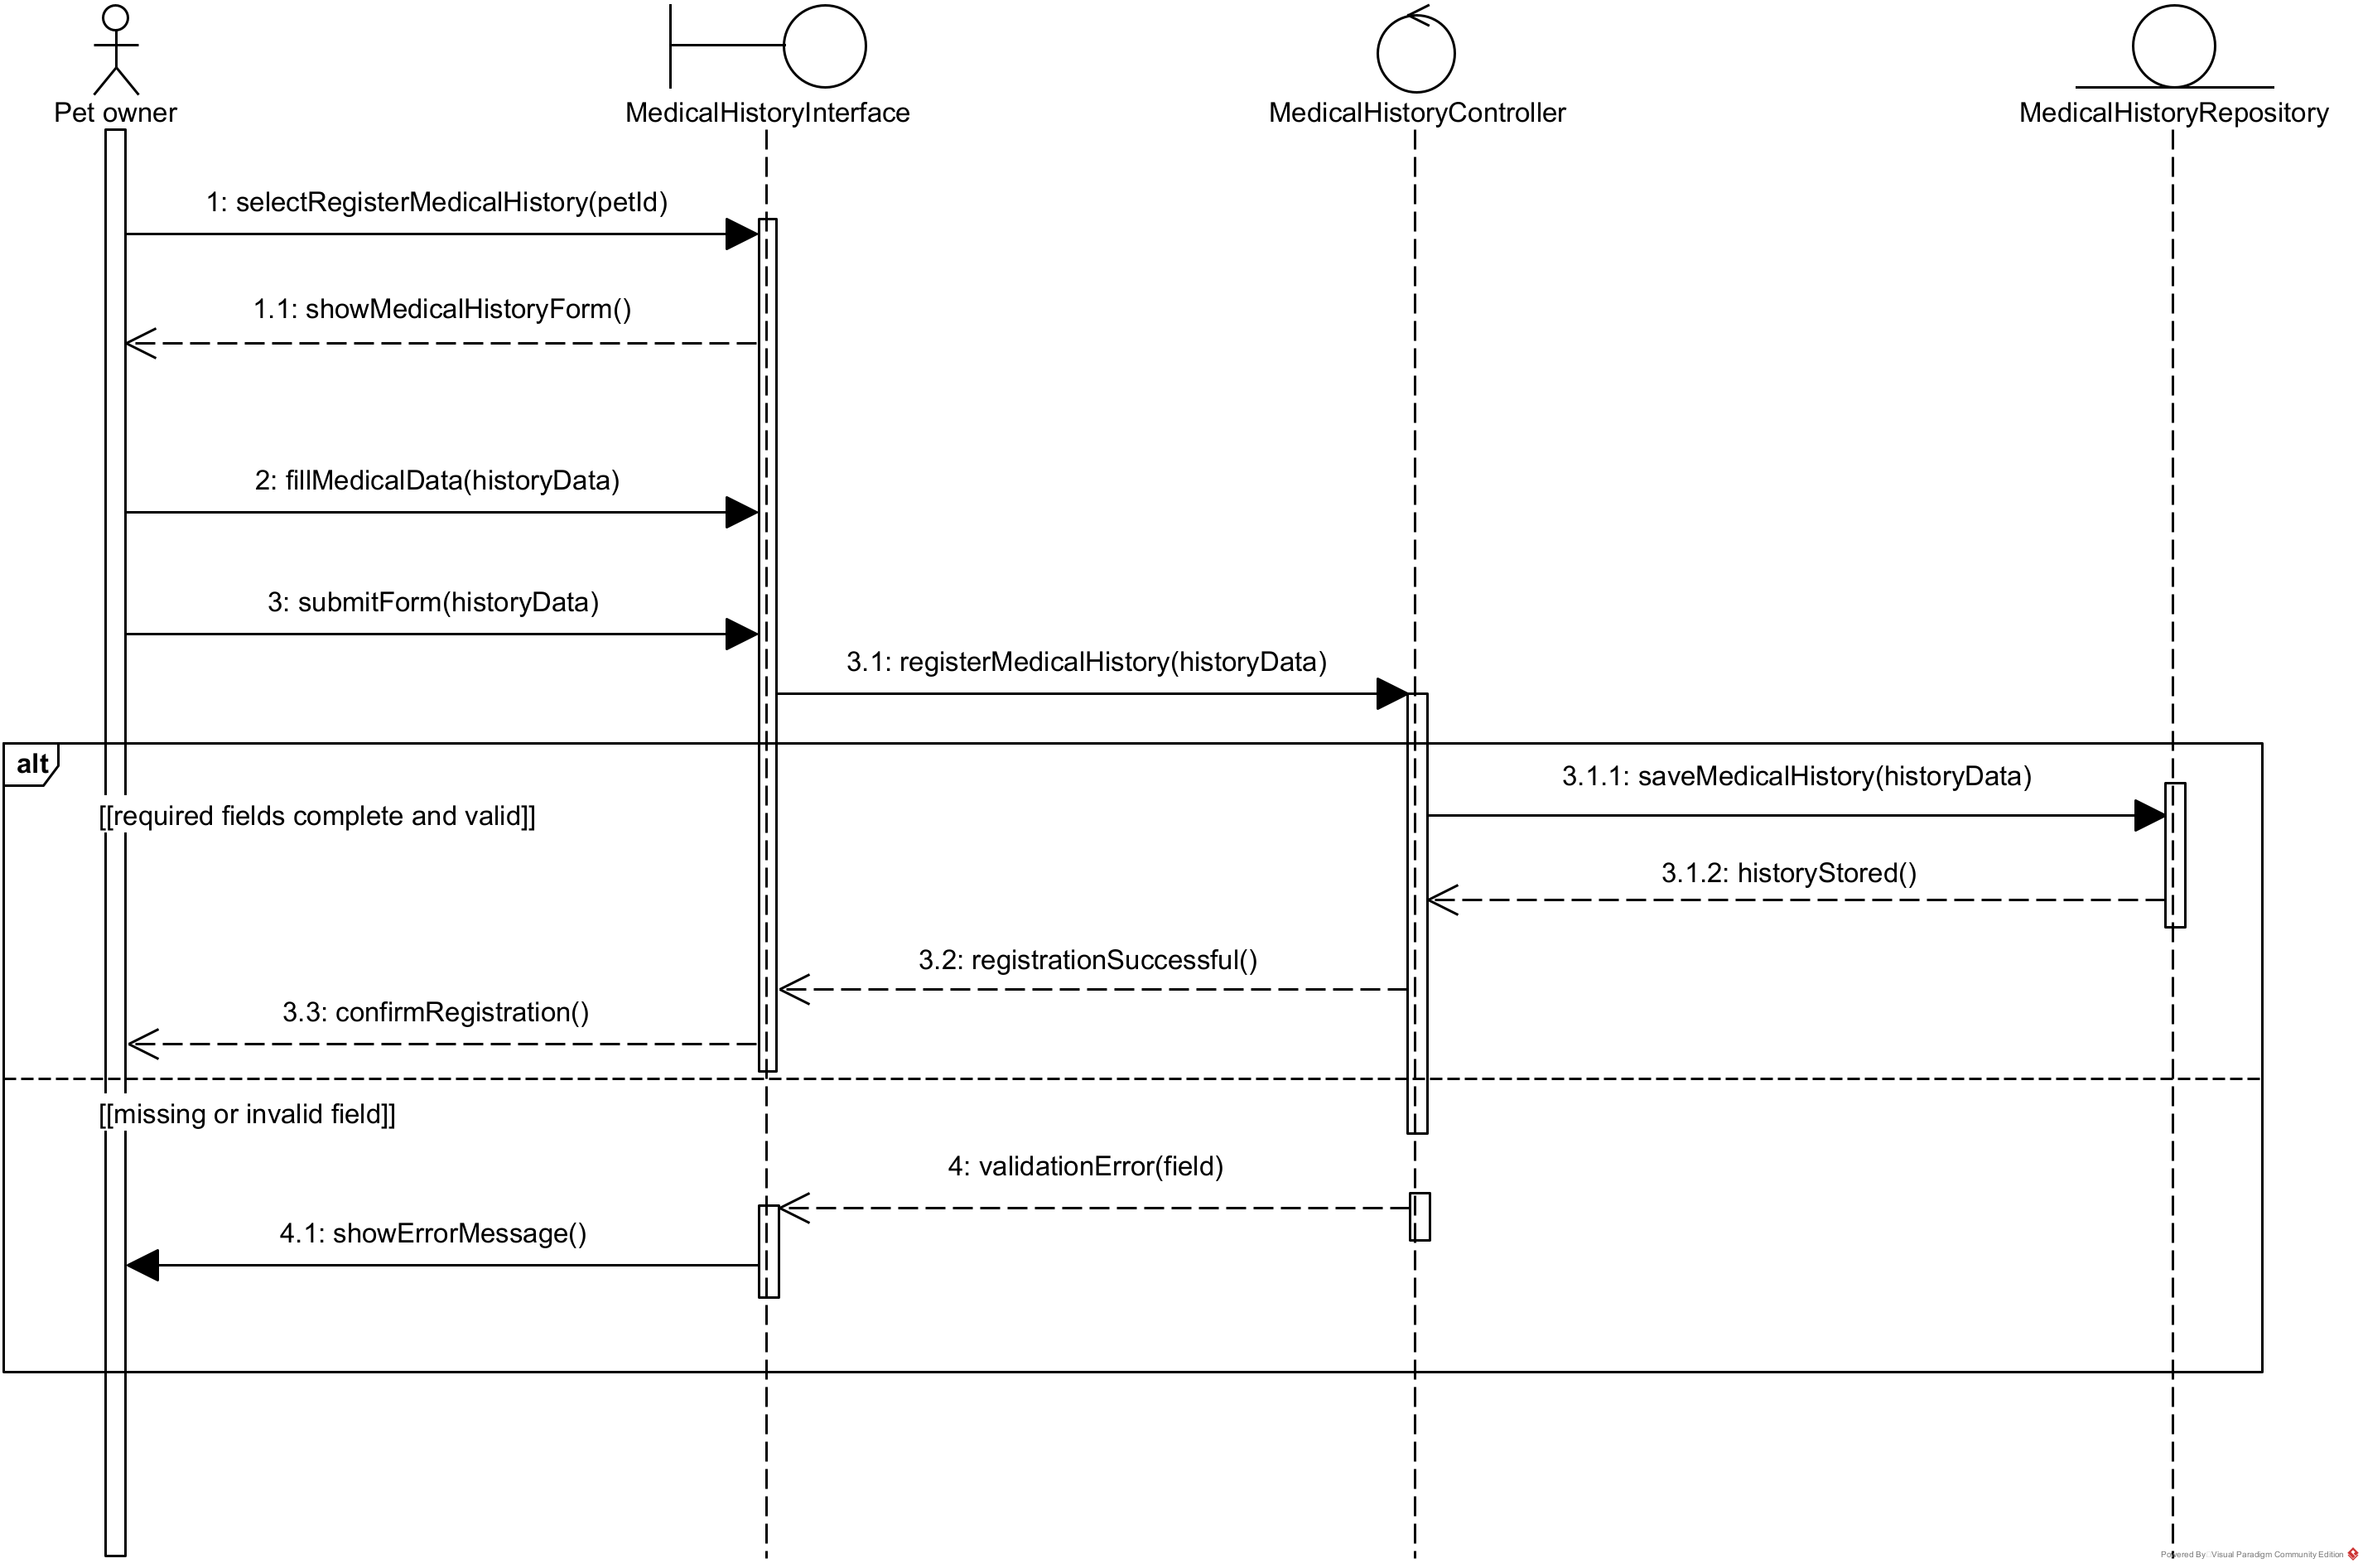
\includegraphics[width=0.72\textwidth]{figuras/DiagramaSecuencia_CU-02_MundiPets.png}
		\caption{Diagrama de secuencia del caso de uso CU-02 --- Registrar historial médico y antecedentes genéticos.}
		\label{fig:sec-cu02}
	\end{figure}

	\subsubsection{Cargar documento veterinario y carnet de vacunación (CU-03)}

	El diagrama de secuencia de CU-03 detalla la carga de documentos
	veterinarios digitalizados (RF-14). El propietario adjunta el archivo; el
	controlador (\texttt{VetDocumentController}) valida el formato y el tamaño
	antes de almacenarlo en el servicio externo de archivos
	(\texttt{FileStorageService}) y de registrar los metadatos del documento en
	el repositorio. Si el archivo no cumple el formato o el tamaño permitido,
	el sistema rechaza la carga y muestra el motivo sin llegar a invocar el
	almacenamiento externo; la validación posterior por parte de una
	veterinaria autorizada queda representada en el diagrama de estados de
	verificación de documentos médicos (Sección~\ref{sec:estados}) y no en
	esta secuencia.

	\begin{figure}[H]
		\centering
		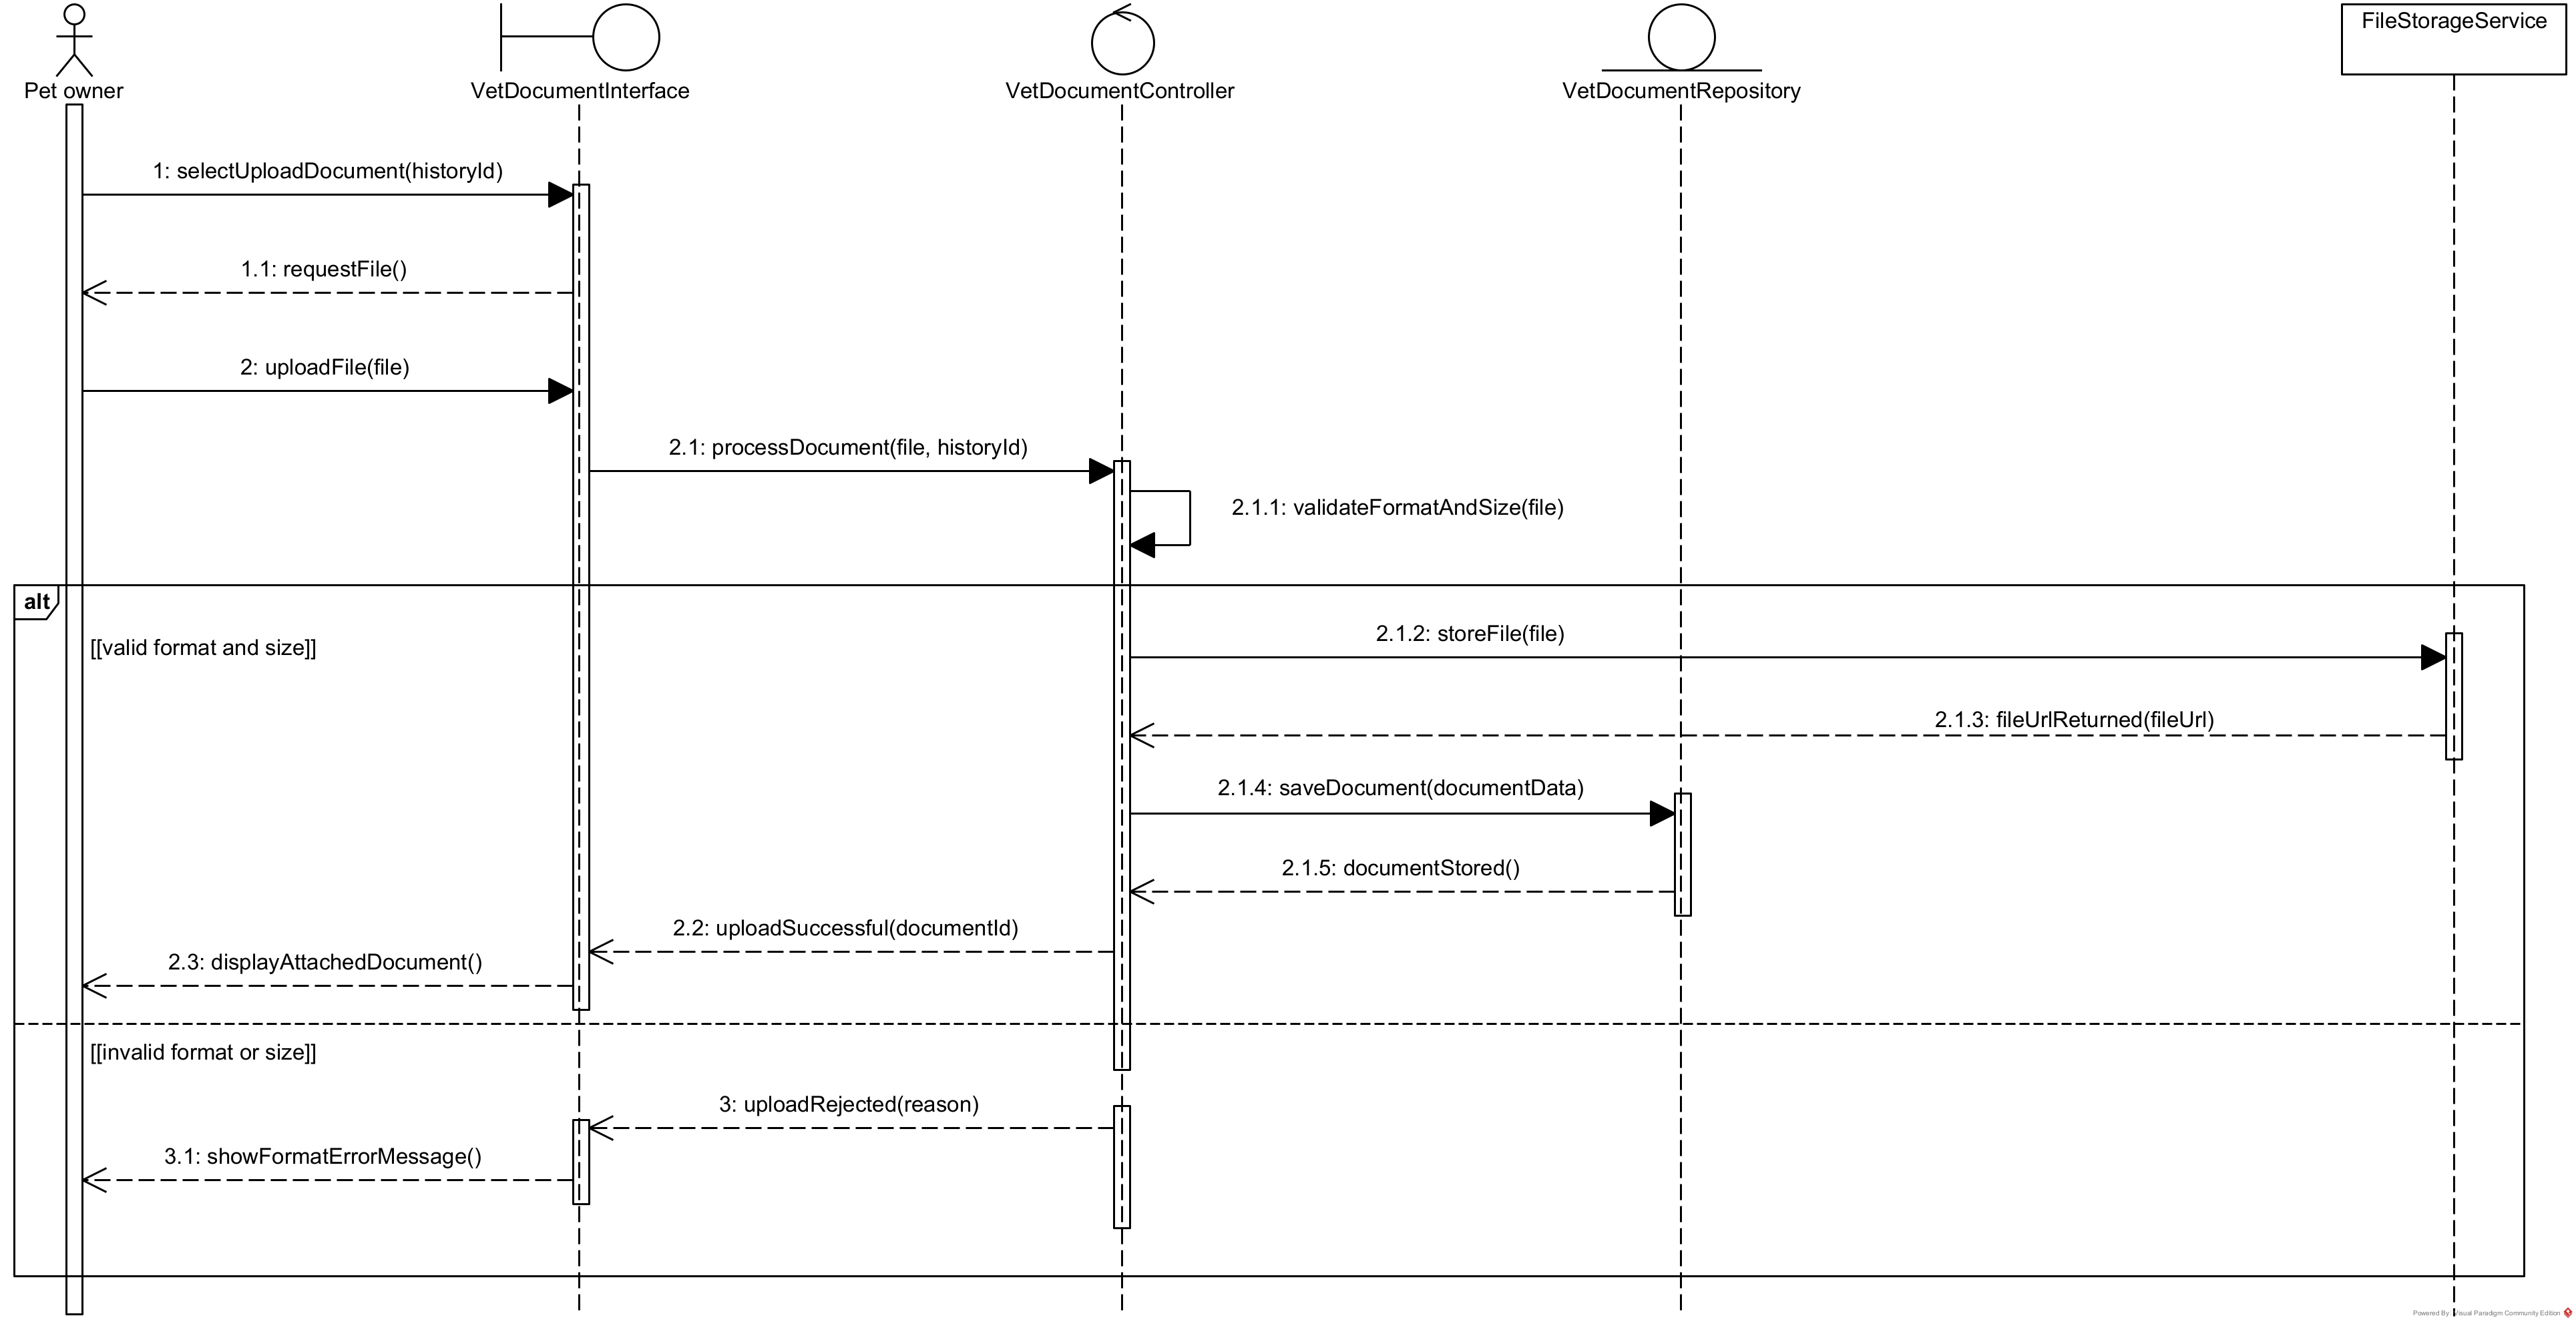
\includegraphics[width=0.72\textwidth]{figuras/DiagramaSecuencia_CU-03_MundiPets.png}
		\caption{Diagrama de secuencia del caso de uso CU-03 --- Cargar documento veterinario y carnet de vacunación.}
		\label{fig:sec-cu03}
	\end{figure}

	\subsubsection{Publicar mascota en adopción (CU-04)}

	El diagrama de secuencia de CU-04 representa el proceso de publicación
	descrito en RF-13. Antes de crear una publicación nueva, el controlador
	(\texttt{PostController}) verifica si la mascota ya cuenta con una
	publicación de adopción activa (\texttt{findActivePost}); si no existe
	ninguna, crea y almacena la nueva publicación, y si ya existe una activa,
	el sistema evita el duplicado ofreciendo al propietario actualizar la
	publicación existente en lugar de crear una nueva, confirmando en ambos
	casos el resultado al usuario.

	\begin{figure}[H]
		\centering
		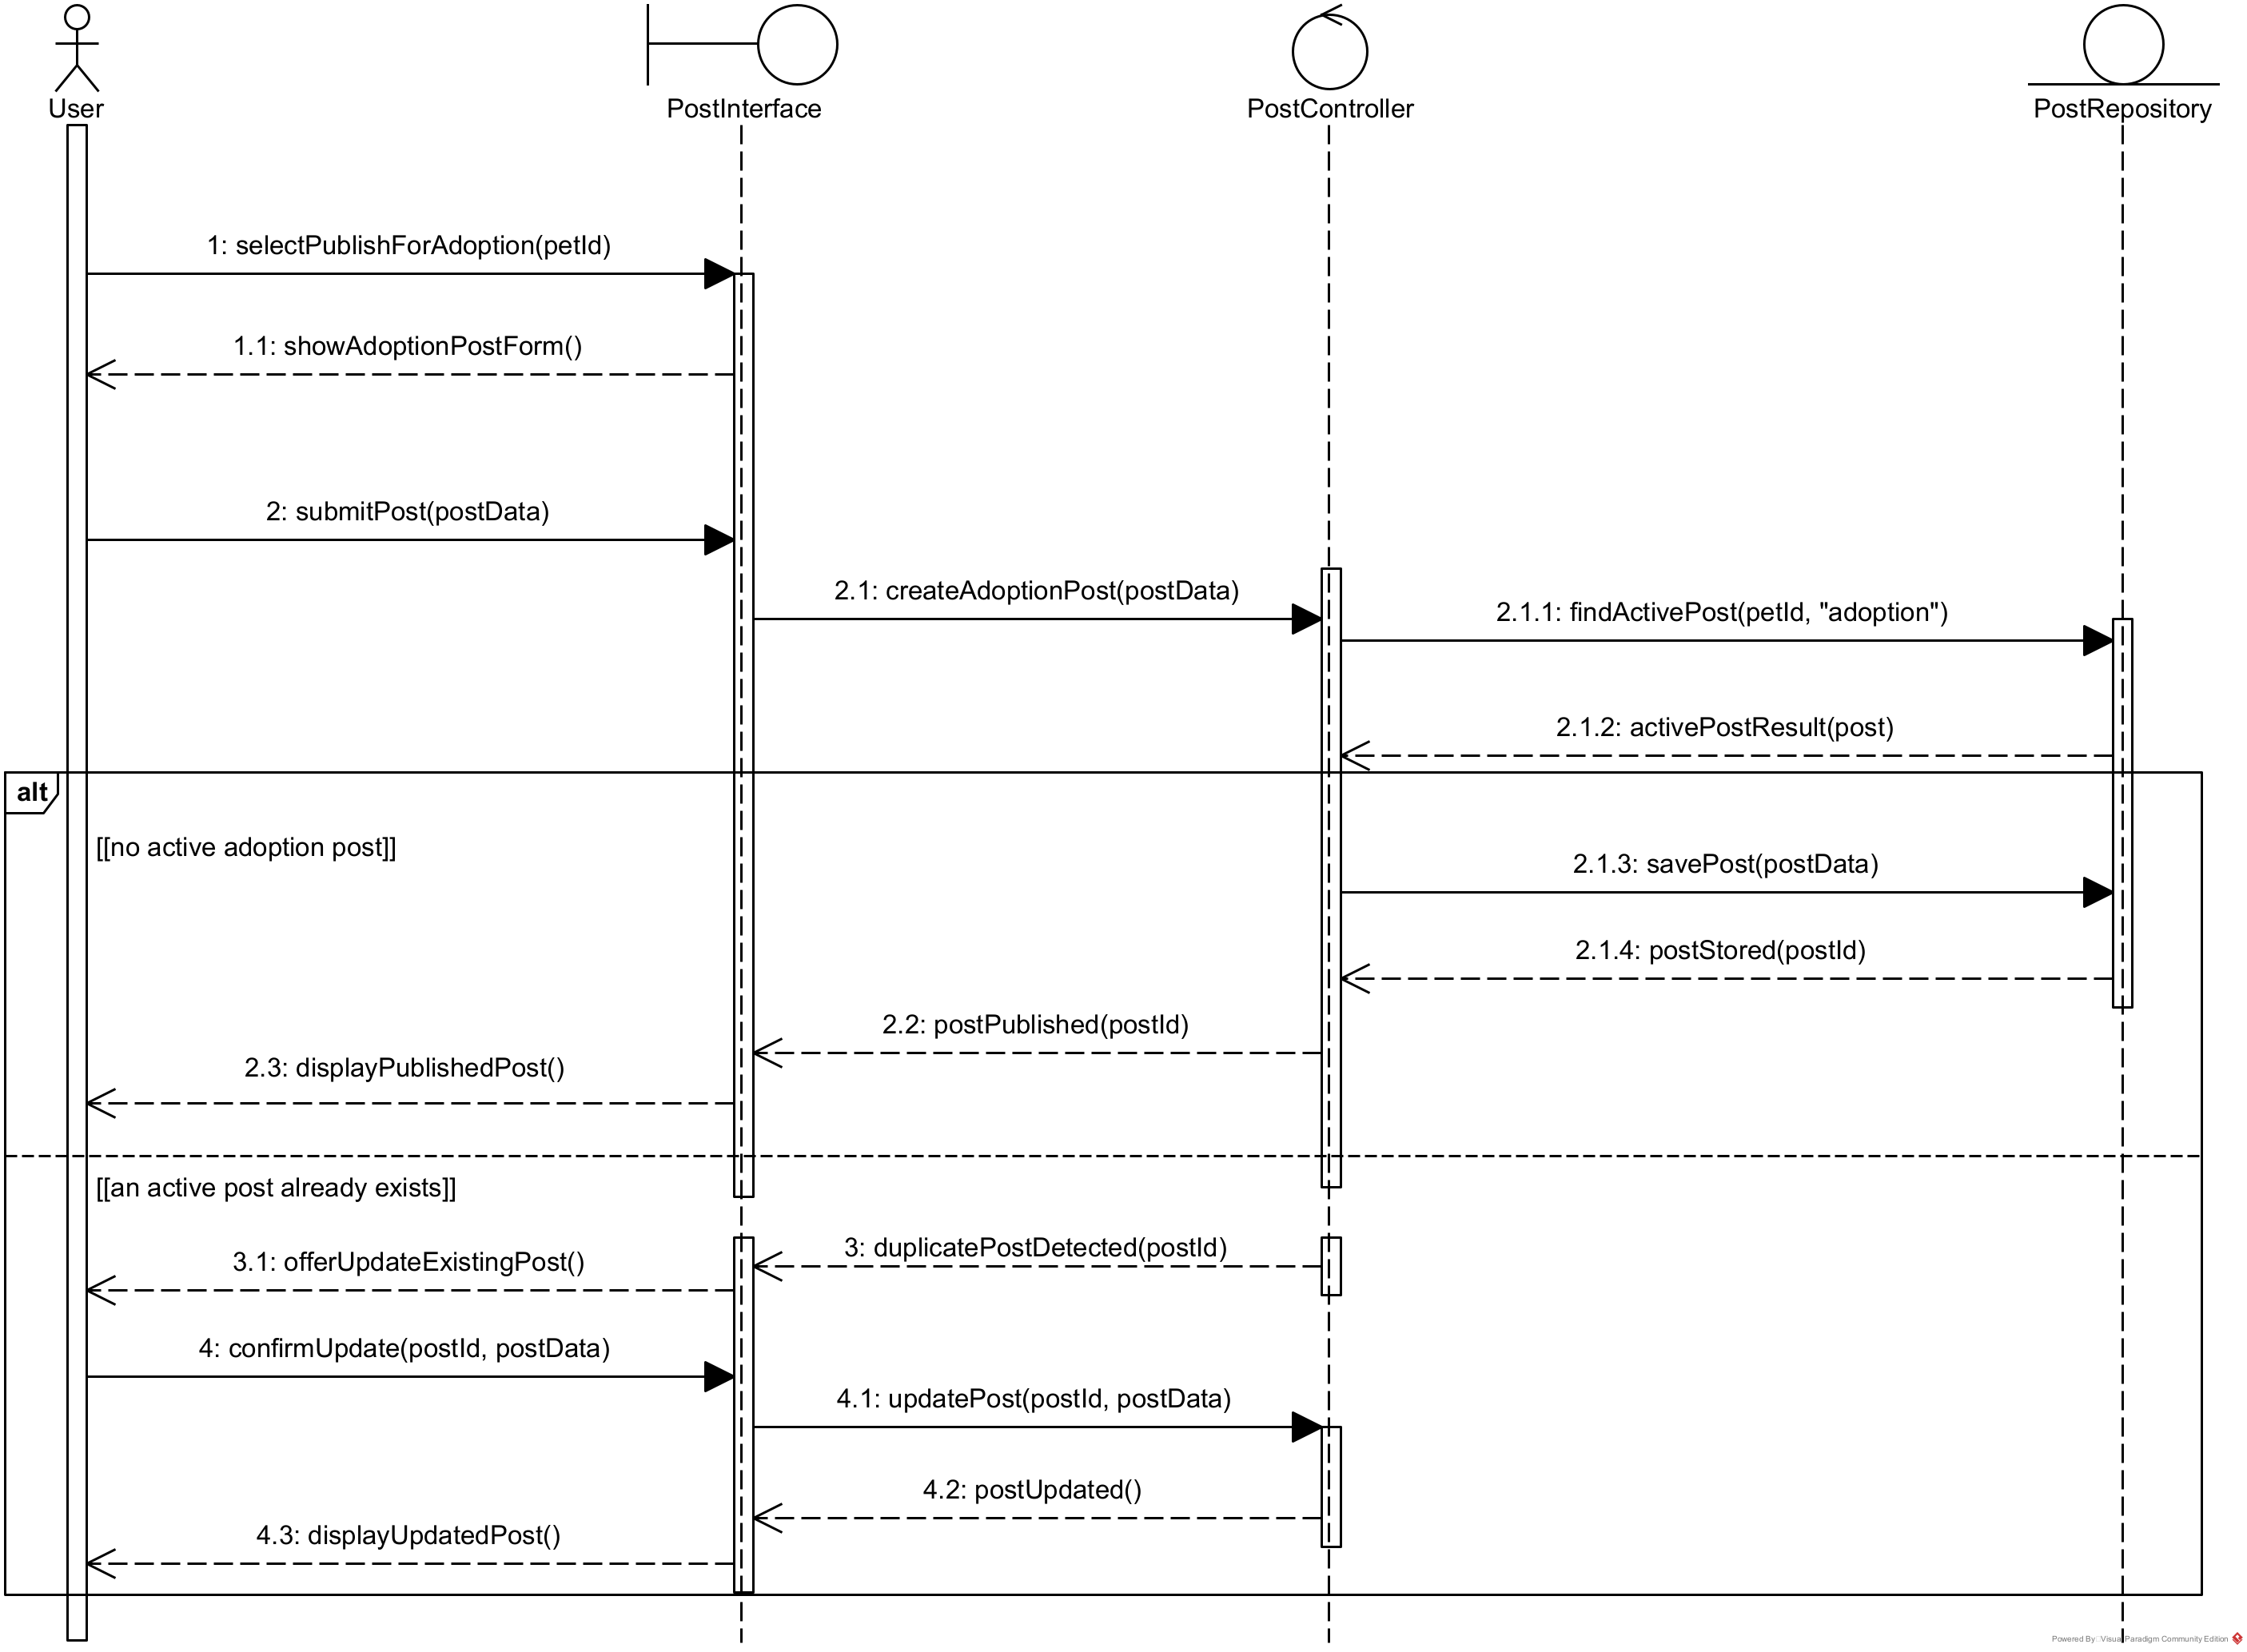
\includegraphics[width=0.72\textwidth]{figuras/DiagramaSecuencia_CU-04_MundiPets.png}
		\caption{Diagrama de secuencia del caso de uso CU-04 --- Publicar mascota en adopción.}
		\label{fig:sec-cu04}
	\end{figure}

	\subsubsection{Publicar mascota para cruza y gestionar solicitud (CU-05)}

	Esta secuencia cubre específicamente la publicación de una mascota
	disponible para cruza responsable (RF-08, RF-13). Antes de crear la
	publicación, el controlador (\texttt{PostController}) obtiene los
	antecedentes genéticos de la mascota (\texttt{getGeneticBackground}); si
	el antecedente no está registrado, el sistema rechaza la publicación y
	solicita al propietario completarlo primero, en cumplimiento de RF-16, y
	solo si el antecedente existe procede a almacenar la publicación y
	confirmarla. La gestión posterior de la solicitud recibida de un
	interesado en cruza --- su aceptación o rechazo por parte del propietario
	receptor --- y la regla de negocio de RF-27 sobre solicitudes repetitivas
	no quedan representadas en este diagrama de publicación, sino en el flujo
	de gestión de solicitudes descrito a continuación (CU-07, según el
	contenido real de su archivo) y en la máquina de estados de la
	Sección~\ref{sec:estados}.

	\begin{figure}[H]
		\centering
		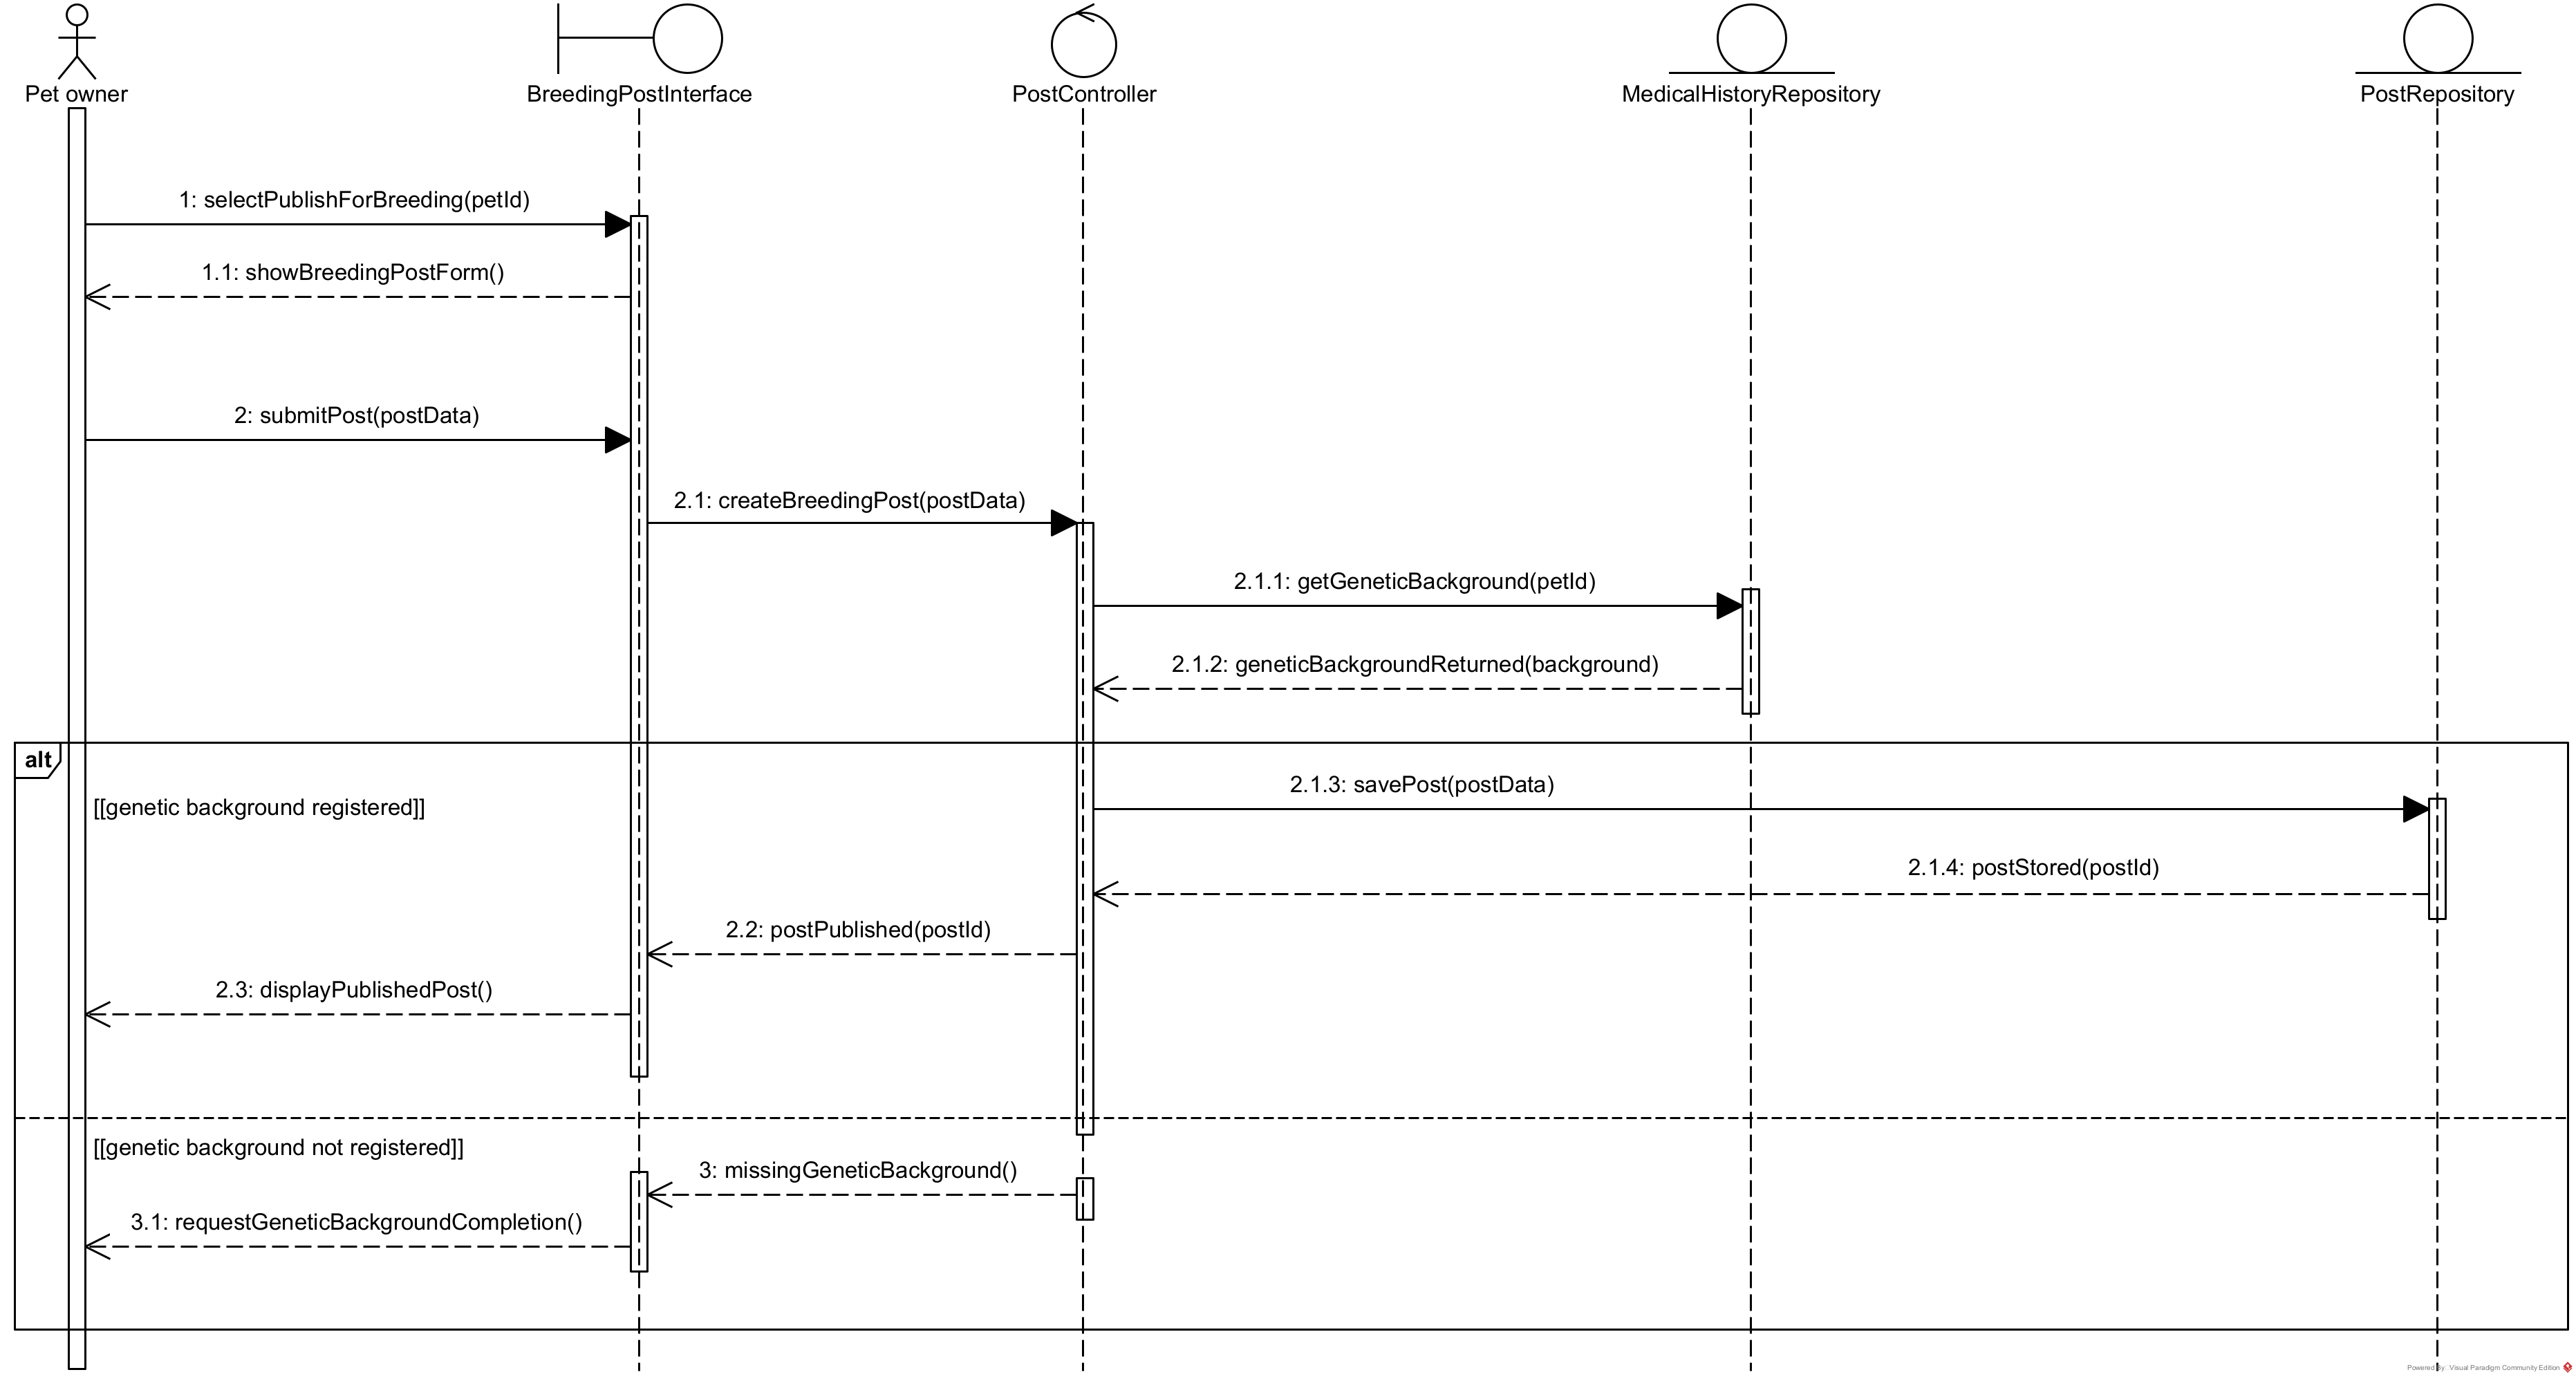
\includegraphics[width=0.72\textwidth]{figuras/DiagramaSecuencia_CU-05_MundiPets.png}
		\caption{Diagrama de secuencia del caso de uso CU-05 --- Publicar mascota para cruza.}
		\label{fig:sec-cu05}
	\end{figure}

	\subsubsection{Configurar privacidad médica (contenido real del archivo CU-06)}

	El archivo \texttt{DiagramaSecuencia\_CU-06} representa la administración
	de la privacidad de la información descrita en RF-11 (especificada como
	CU-12 en la Sección~\ref{sec:cu-detallado}; véase la nota de verificación
	al inicio de esta subsección). El propietario consulta las opciones de
	visibilidad disponibles y selecciona las reglas para cada categoría de
	dato; antes de guardar, el controlador (\texttt{PrivacyController})
	ejecuta \texttt{checkMandatoryVetFields()} para impedir que se restrinja
	por completo un campo médico obligatorio para la validación veterinaria
	exigida por RD-03, devolviendo una advertencia específica si se intenta
	ocultar ese campo en particular, mientras que el resto de la configuración
	se guarda con normalidad.

	\begin{figure}[H]
		\centering
		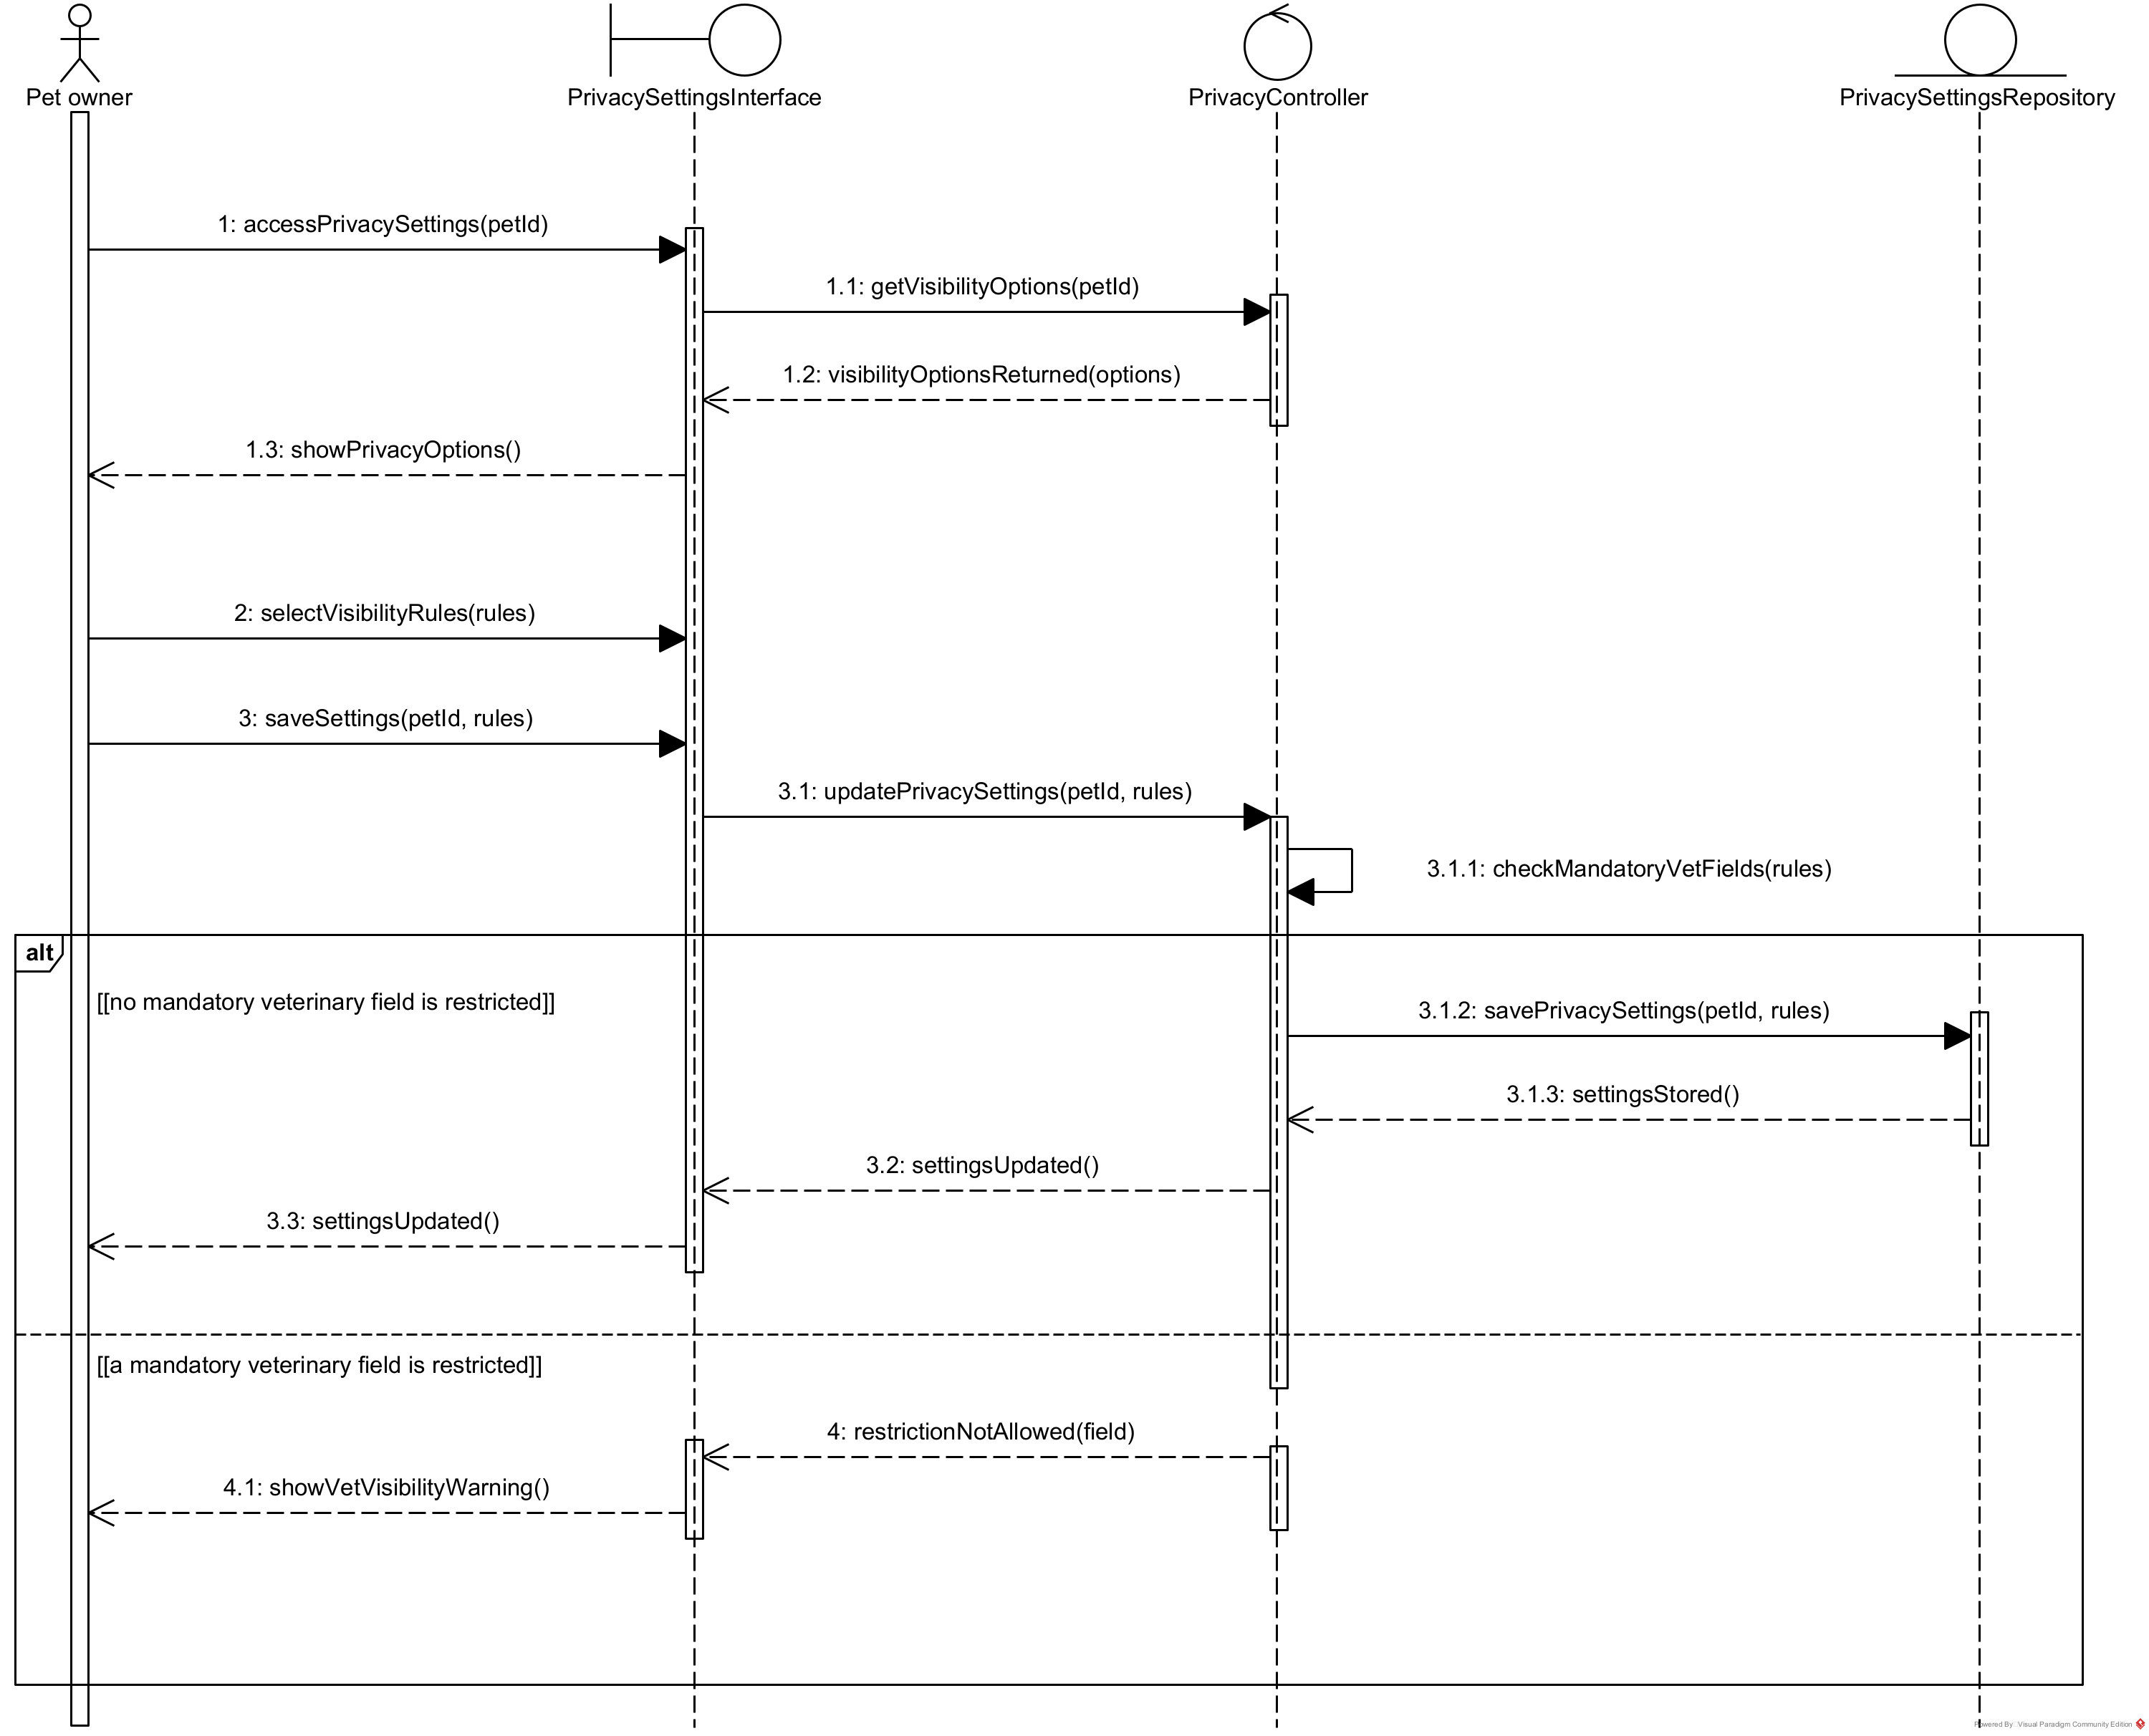
\includegraphics[width=0.72\textwidth]{figuras/DiagramaSecuencia_CU-06_MundiPets.png}
		\caption{Diagrama de secuencia --- Configurar privacidad médica (archivo etiquetado CU-06; corresponde a CU-12).}
		\label{fig:sec-cu06}
	\end{figure}

	\subsubsection{Gestionar solicitud de adopción (contenido real del archivo CU-07)}

	El archivo \texttt{DiagramaSecuencia\_CU-07} representa la gestión de una
	solicitud de adopción ya enviada (RF-05, RF-18), complementando la
	publicación cubierta por CU-04. El adoptante consulta el perfil (CU-10) y
	envía la solicitud, que el sistema registra en estado \emph{pending} y
	notifica al propietario o refugio receptor; este revisa la solicitud y
	decide aceptarla o rechazarla, y el sistema actualiza el estado
	correspondiente y notifica al adoptante en ambos casos. Esta secuencia es
	la contraparte, para adopción, de la gestión de solicitud de cruza descrita
	en el flujo alterno de CU-05.

	\begin{figure}[H]
		\centering
		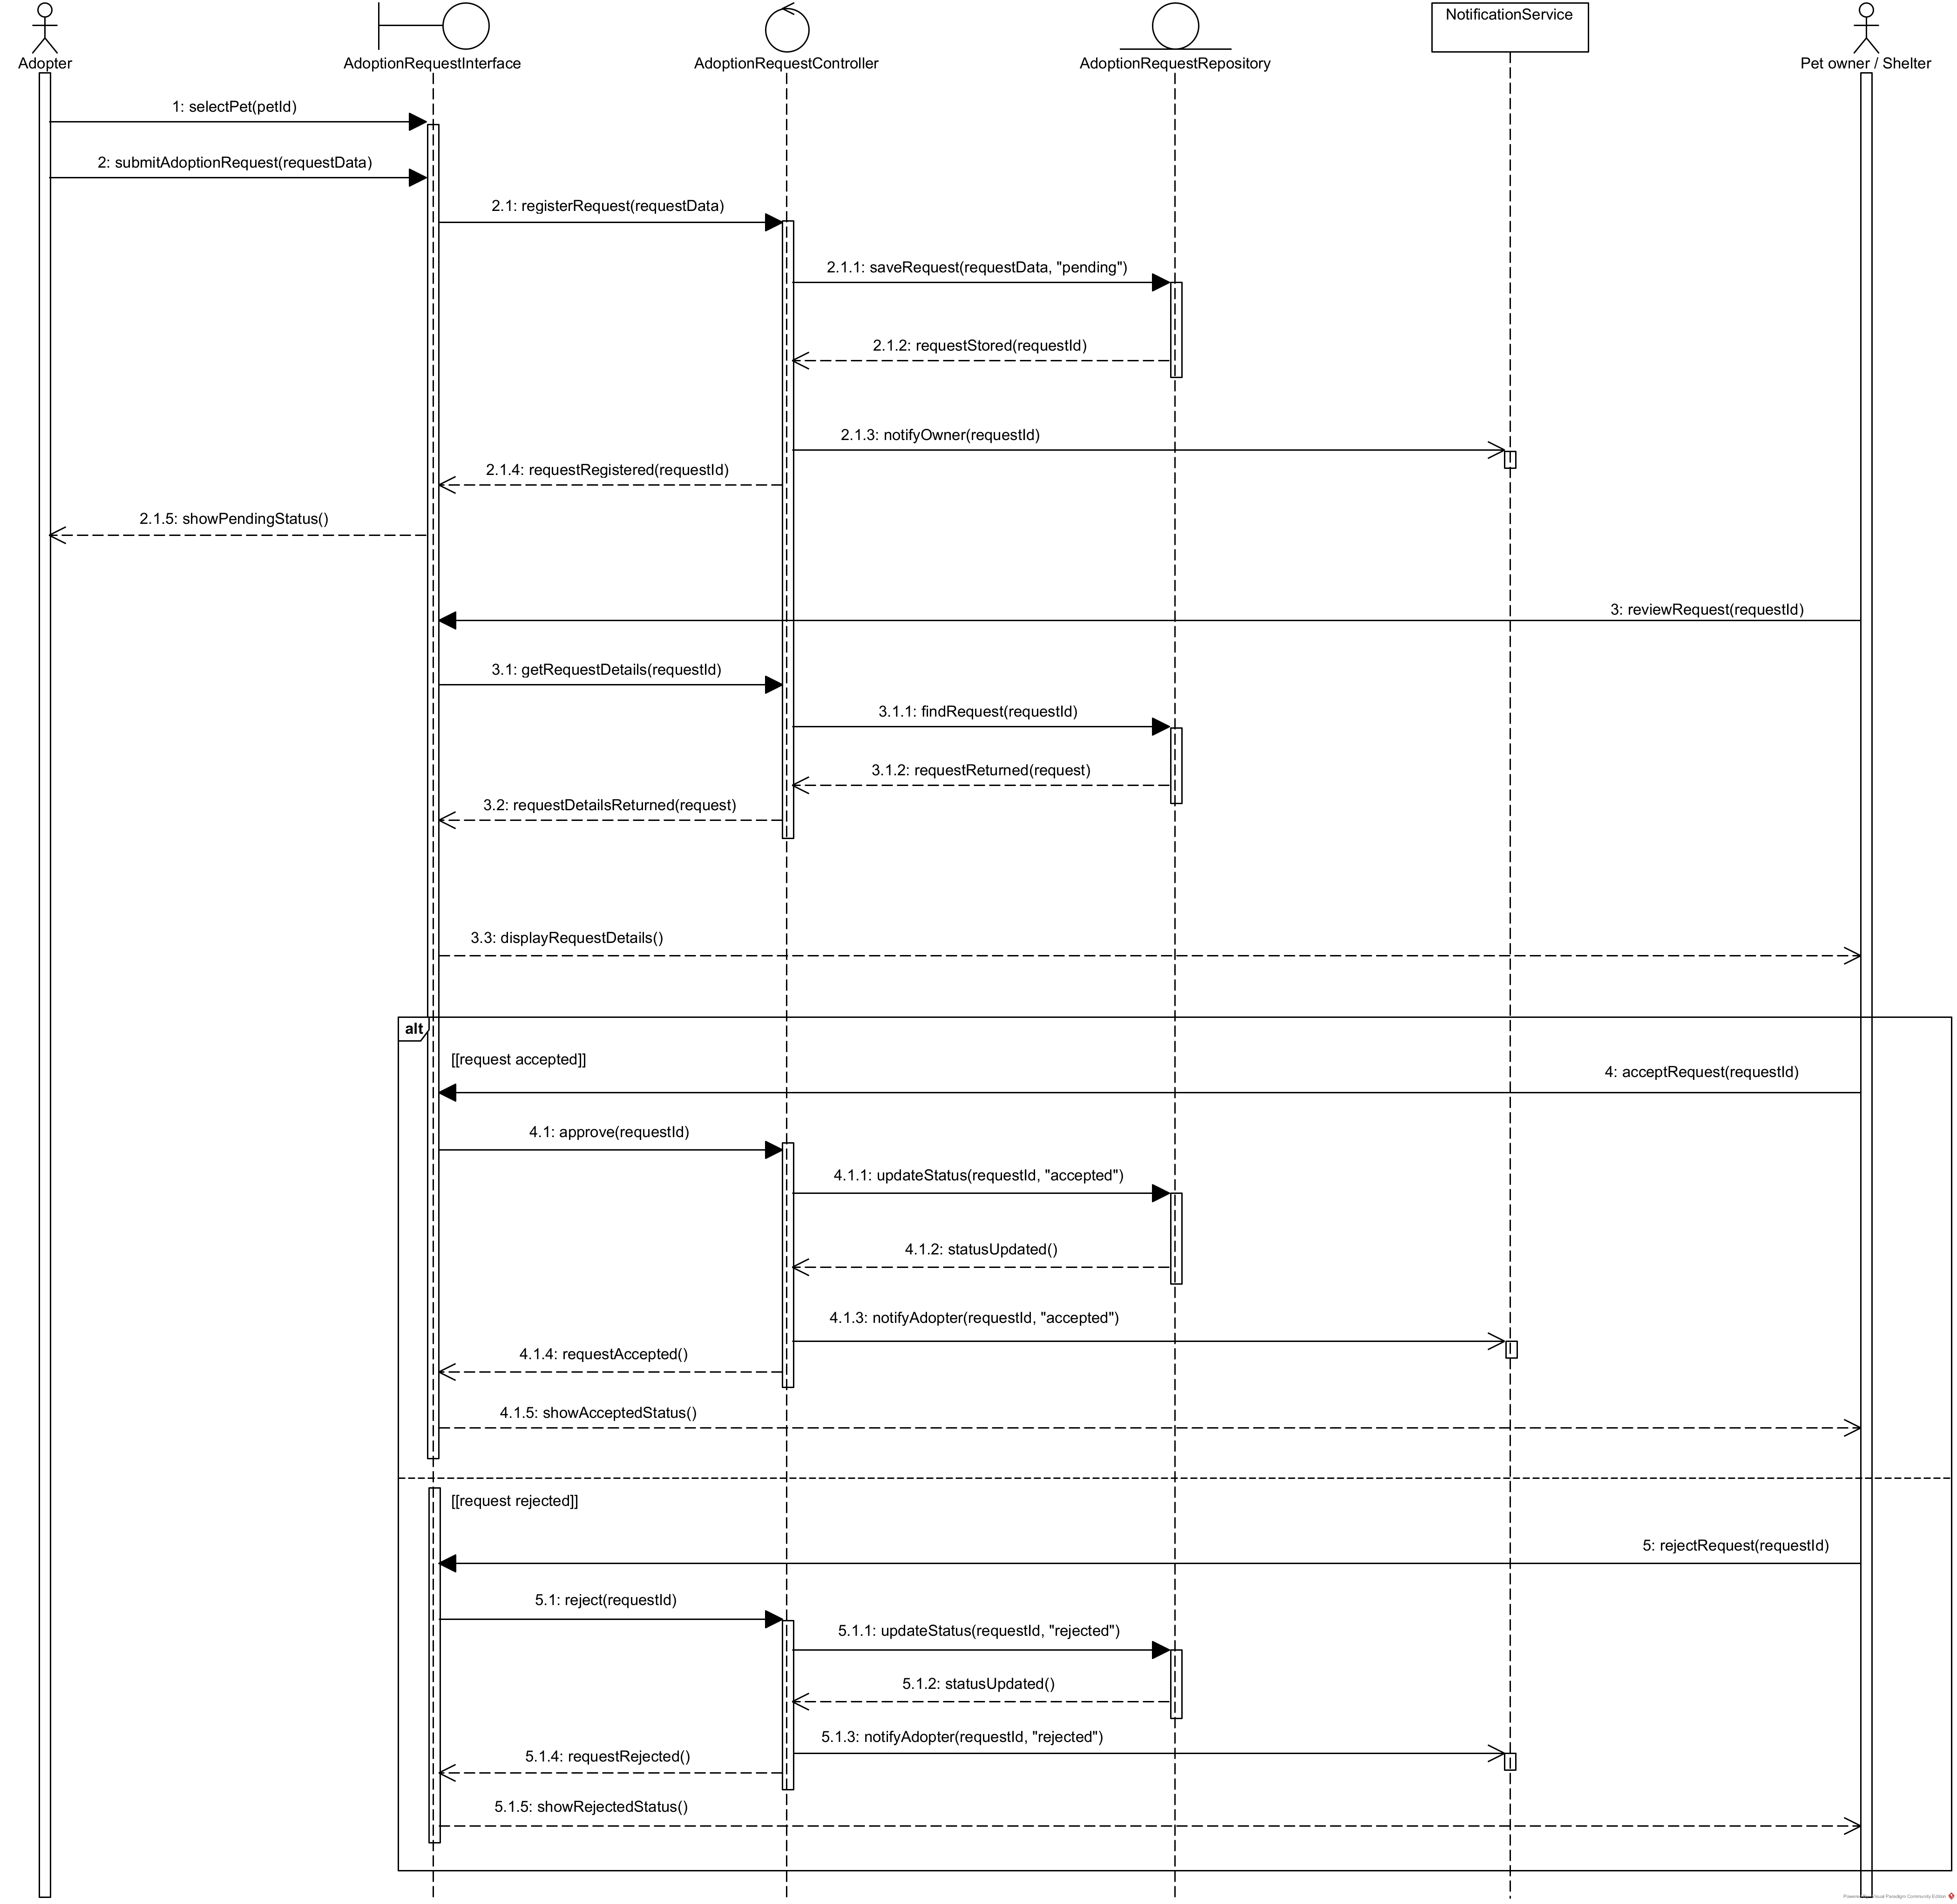
\includegraphics[width=0.72\textwidth]{figuras/DiagramaSecuencia_CU-07_MundiPets.png}
		\caption{Diagrama de secuencia --- Gestionar solicitud de adopción (archivo etiquetado CU-07).}
		\label{fig:sec-cu07}
	\end{figure}

	\subsubsection{Gestionar comunicación entre usuarios (CU-08)}

	Esta secuencia representa el intercambio de mensajes entre usuarios
	(RF-07). El remitente selecciona al destinatario y envía el mensaje; el
	controlador (\texttt{MessageController}) busca la conversación existente
	entre ambos o crea una nueva si es la primera interacción
	(\texttt{opt~[no~previous~conversation~registered]}), almacena el mensaje
	y notifica al receptor mediante el servicio de notificaciones. El diagrama
	no representa de forma explícita el paso por un componente de moderación
	automática ni la bifurcación de bloqueo por contenido inapropiado; la
	explicación por ejemplos exigida por RNF-15 ante un mensaje reportado se
	documenta en la especificación textual de RF-07 y en la ficha de RNF-15,
	no en esta secuencia de envío.

	\begin{figure}[H]
		\centering
		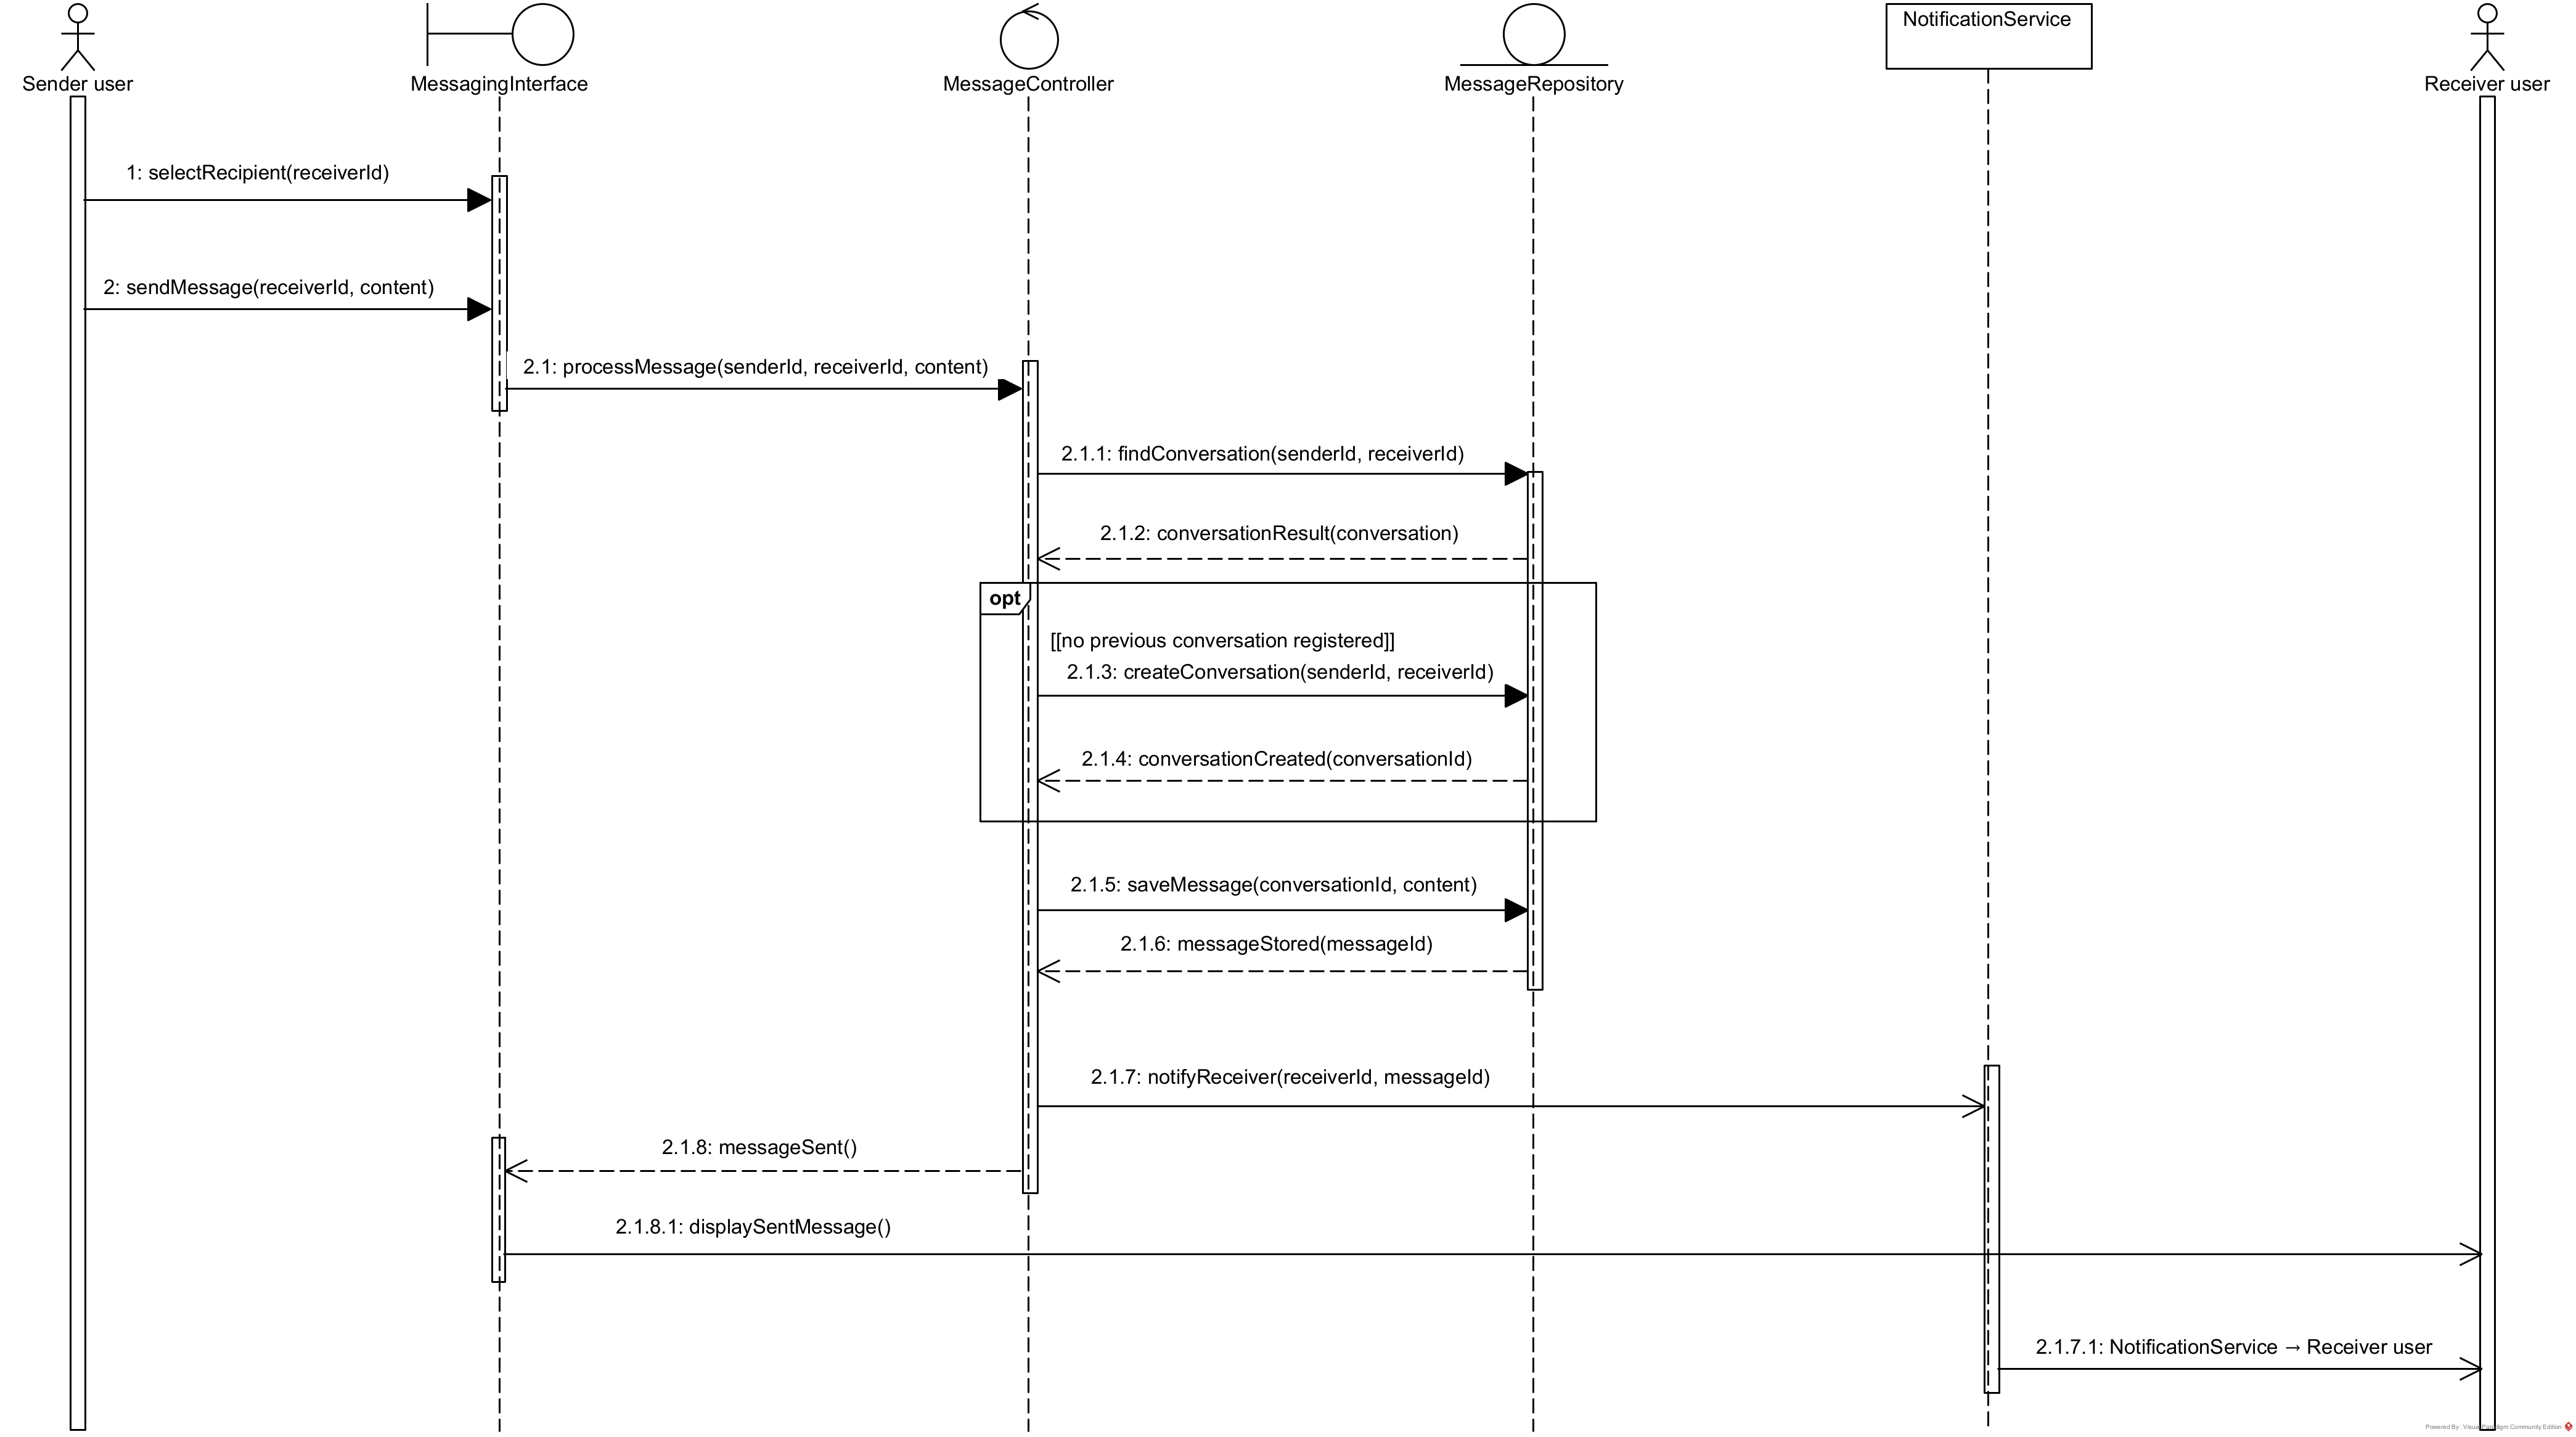
\includegraphics[width=0.72\textwidth]{figuras/DiagramaSecuencia_CU-08_MundiPets.png}
		\caption{Diagrama de secuencia del caso de uso CU-08 --- Gestionar comunicación entre usuarios.}
		\label{fig:sec-cu08}
	\end{figure}

	\subsubsection{Validar información médica (CU-09)}

	El diagrama de secuencia de CU-09 modela la revisión que realiza la
	veterinaria sobre el historial médico y los documentos cargados por el
	propietario (RF-09). El controlador (\texttt{ValidationController}) reúne
	el historial médico y los documentos veterinarios de la mascota antes de
	mostrarlos; la interacción distingue dos caminos alternos: la validación
	exitosa, que marca la información con estado \emph{validated} y la
	identificación de la veterinaria responsable; y el rechazo
	(\texttt{rejectValidation}), que exige registrar el motivo de la
	inconsistencia antes de notificar al propietario. La segunda opinión
	veterinaria de RF-26 se satisface mediante una nueva ejecución de esta
	misma secuencia sobre un registro que ya se encuentra validado, iniciada
	por una veterinaria distinta.

	\begin{figure}[H]
		\centering
		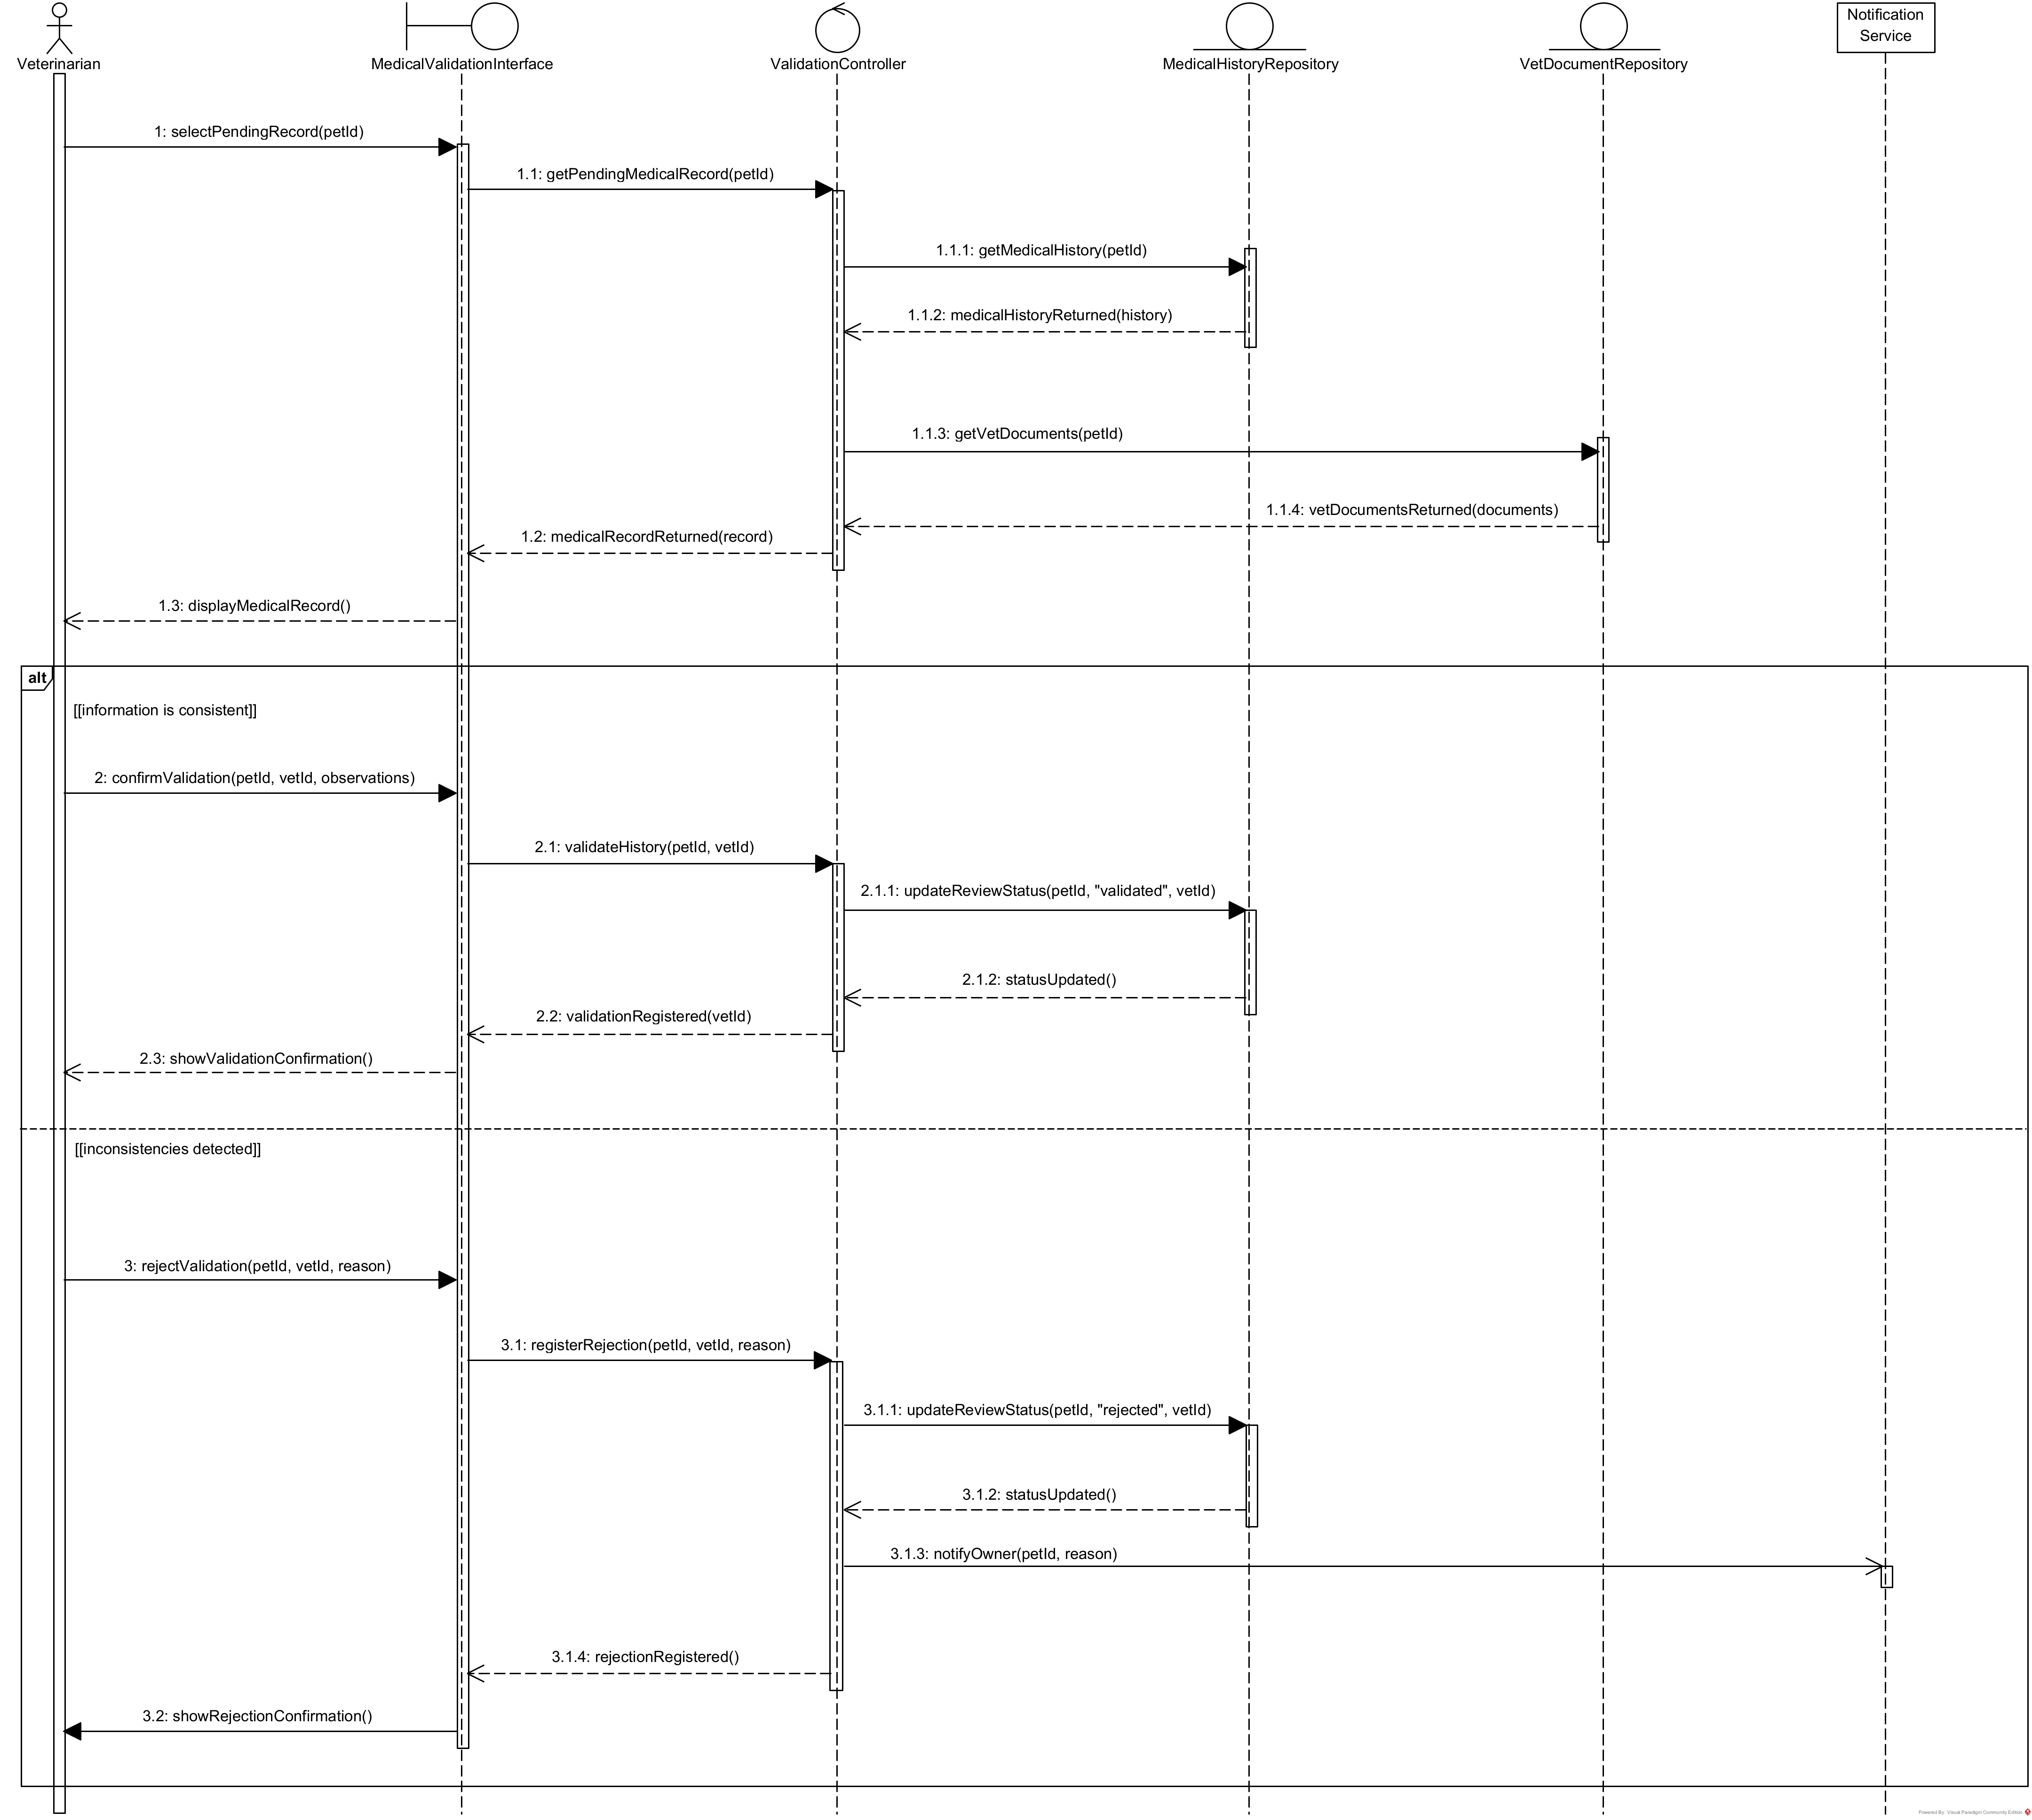
\includegraphics[width=0.72\textwidth]{figuras/DiagramaSecuencia_CU-09_MundiPets.png}
		\caption{Diagrama de secuencia del caso de uso CU-09 --- Validar información médica.}
		\label{fig:sec-cu09}
	\end{figure}

	\subsubsection{Consultar perfil médico (CU-10)}

	Esta secuencia detalla la consulta de perfil completo de una mascota
	(RF-03), incluyendo la aplicación de las reglas de privacidad configuradas
	por el propietario (RF-11). El controlador (\texttt{PetProfileController})
	verifica los permisos de visibilidad del usuario consultante
	(\texttt{checkVisibilityPermissions}) antes de recuperar los datos
	generales y el historial médico de la mascota; si el usuario cuenta con
	permisos completos, recibe el perfil íntegro, y si no los tiene, recibe
	una versión restringida que omite los campos protegidos por la
	configuración de privacidad.

	\begin{figure}[H]
		\centering
		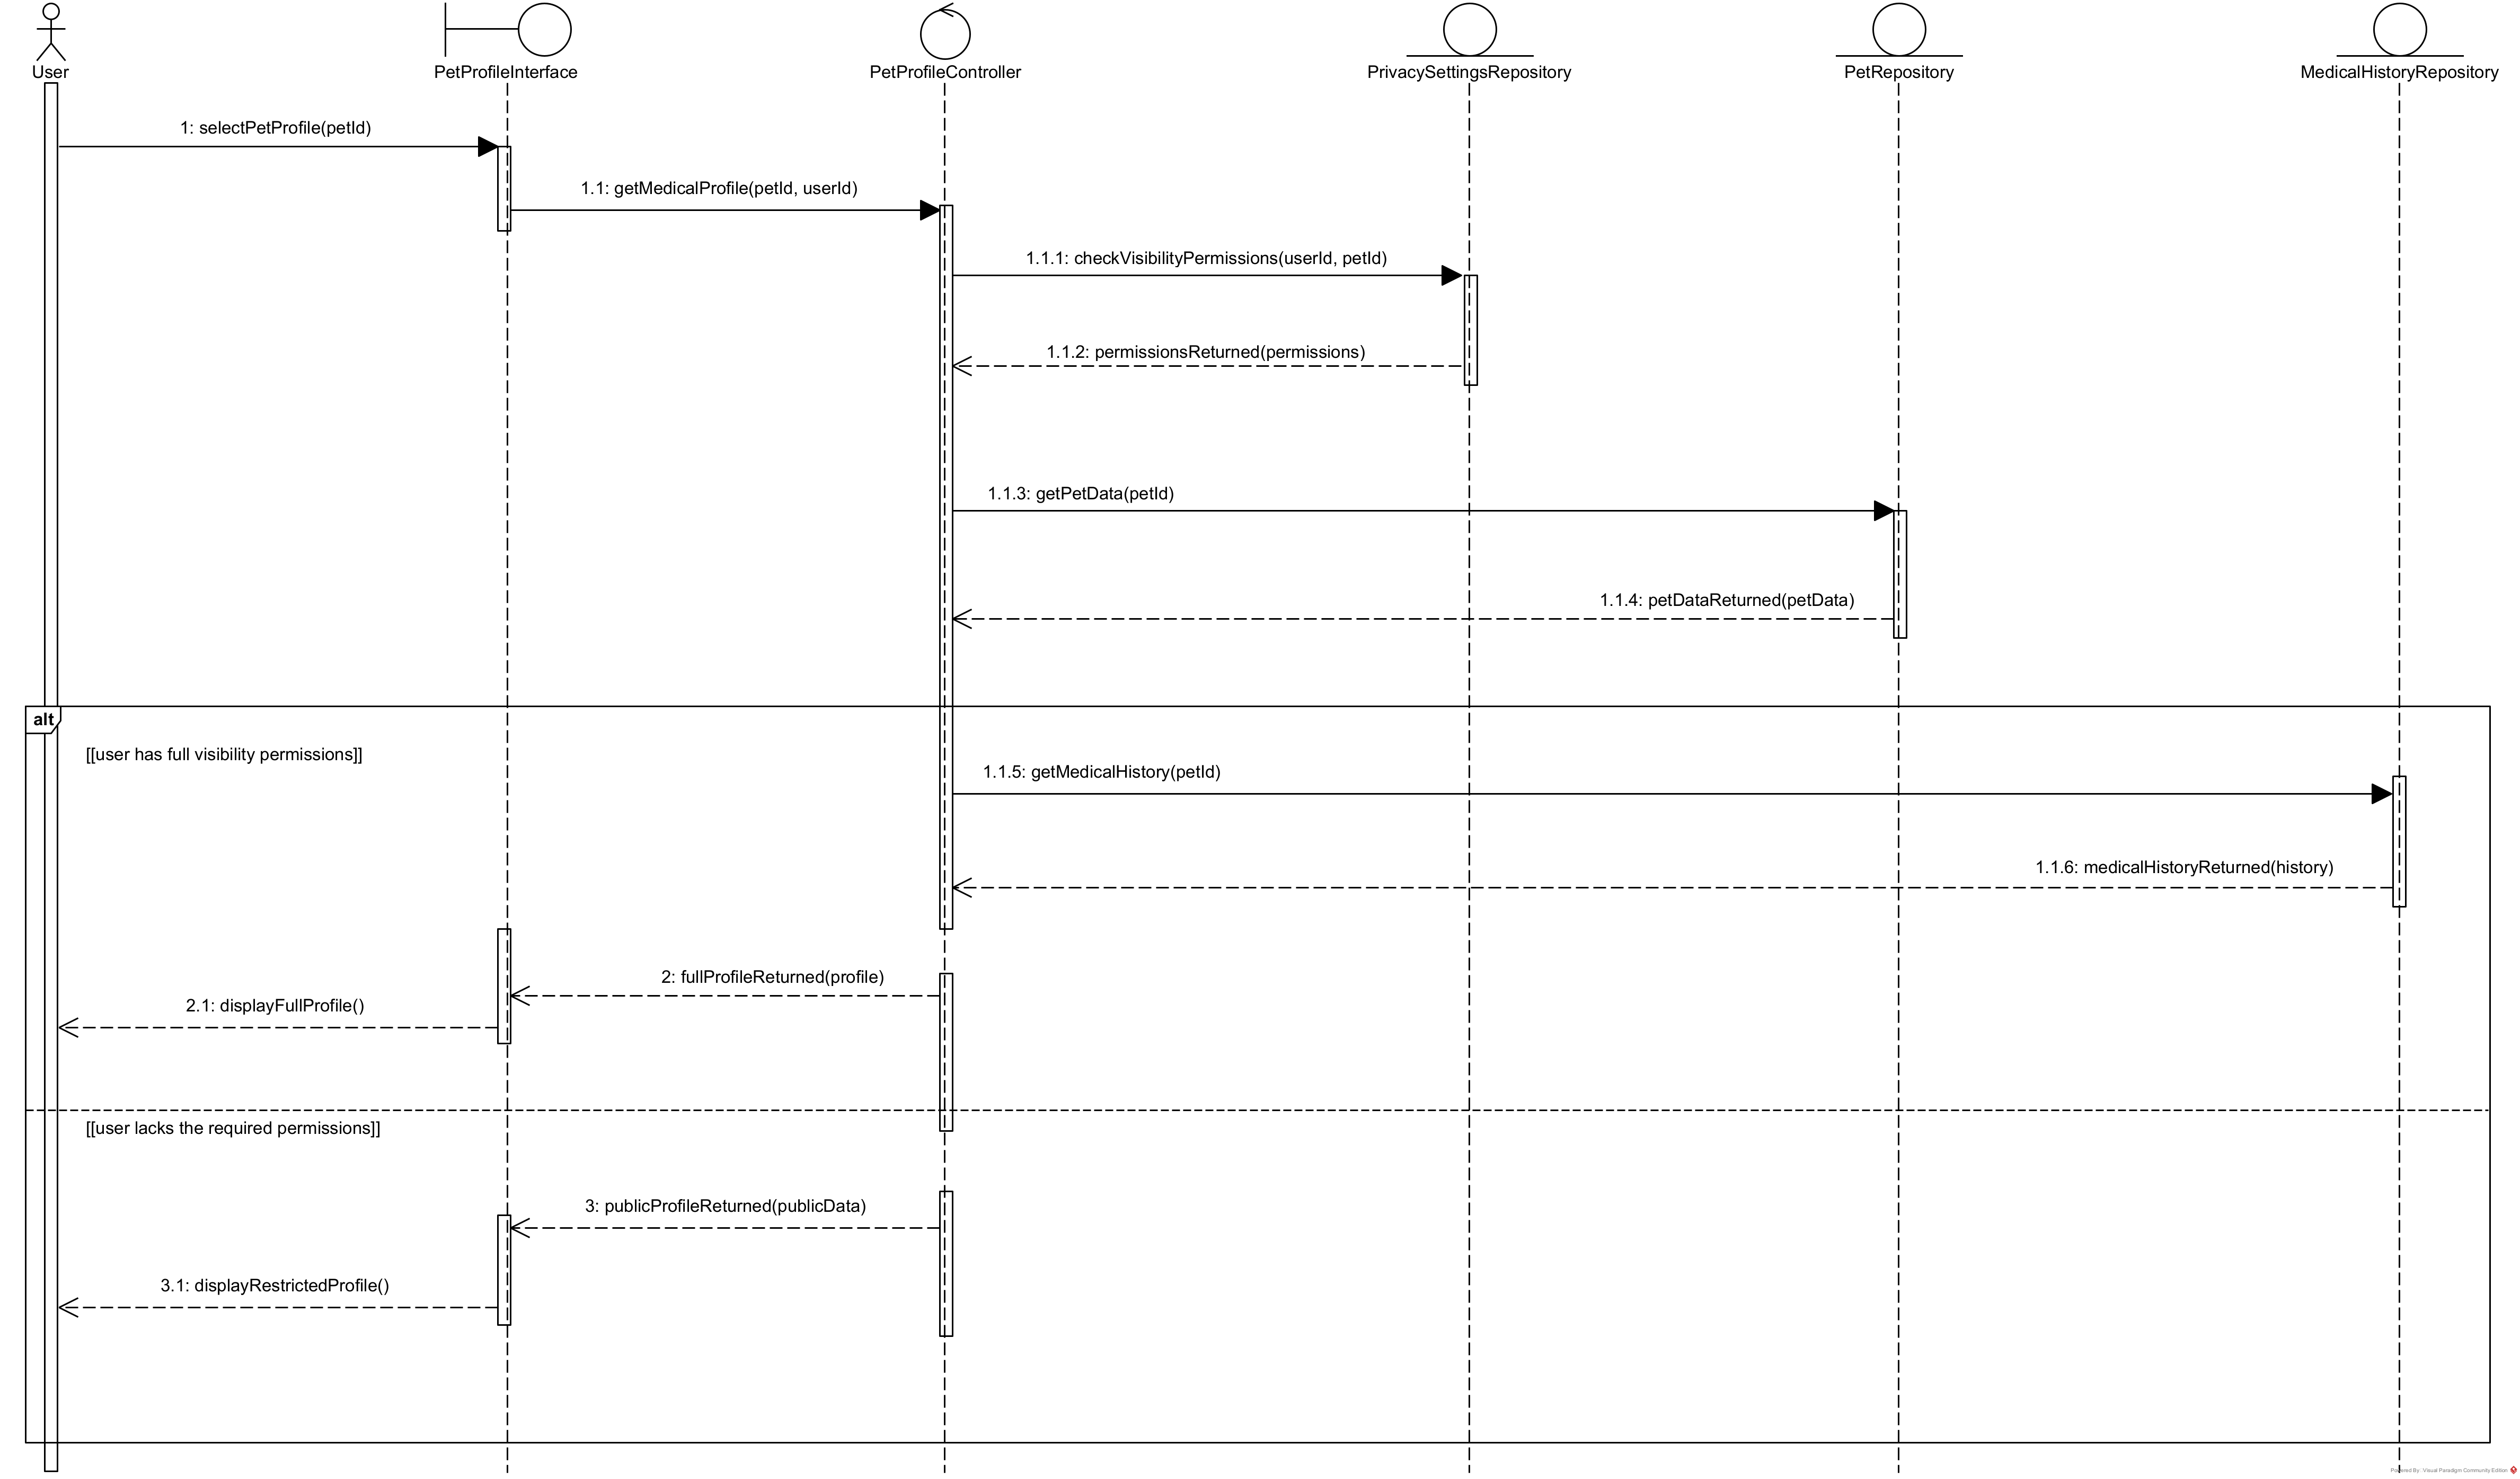
\includegraphics[width=0.72\textwidth]{figuras/DiagramaSecuencia_CU-10_MundiPets.png}
		\caption{Diagrama de secuencia del caso de uso CU-10 --- Consultar perfil médico.}
		\label{fig:sec-cu10}
	\end{figure}

	\subsubsection{Buscar mascota disponible (CU-11)}

	El diagrama de secuencia de CU-11 modela la búsqueda y el filtrado de
	mascotas disponibles (RF-04). El adoptante accede a la búsqueda y aplica
	criterios de filtrado; el controlador (\texttt{SearchController}) consulta
	el repositorio de publicaciones según dichos criterios
	(\texttt{findPostsByCriteria}) y retorna la lista de coincidencias, o bien
	un resultado vacío con el mensaje correspondiente cuando ninguna
	publicación cumple los filtros aplicados.

	\begin{figure}[H]
		\centering
		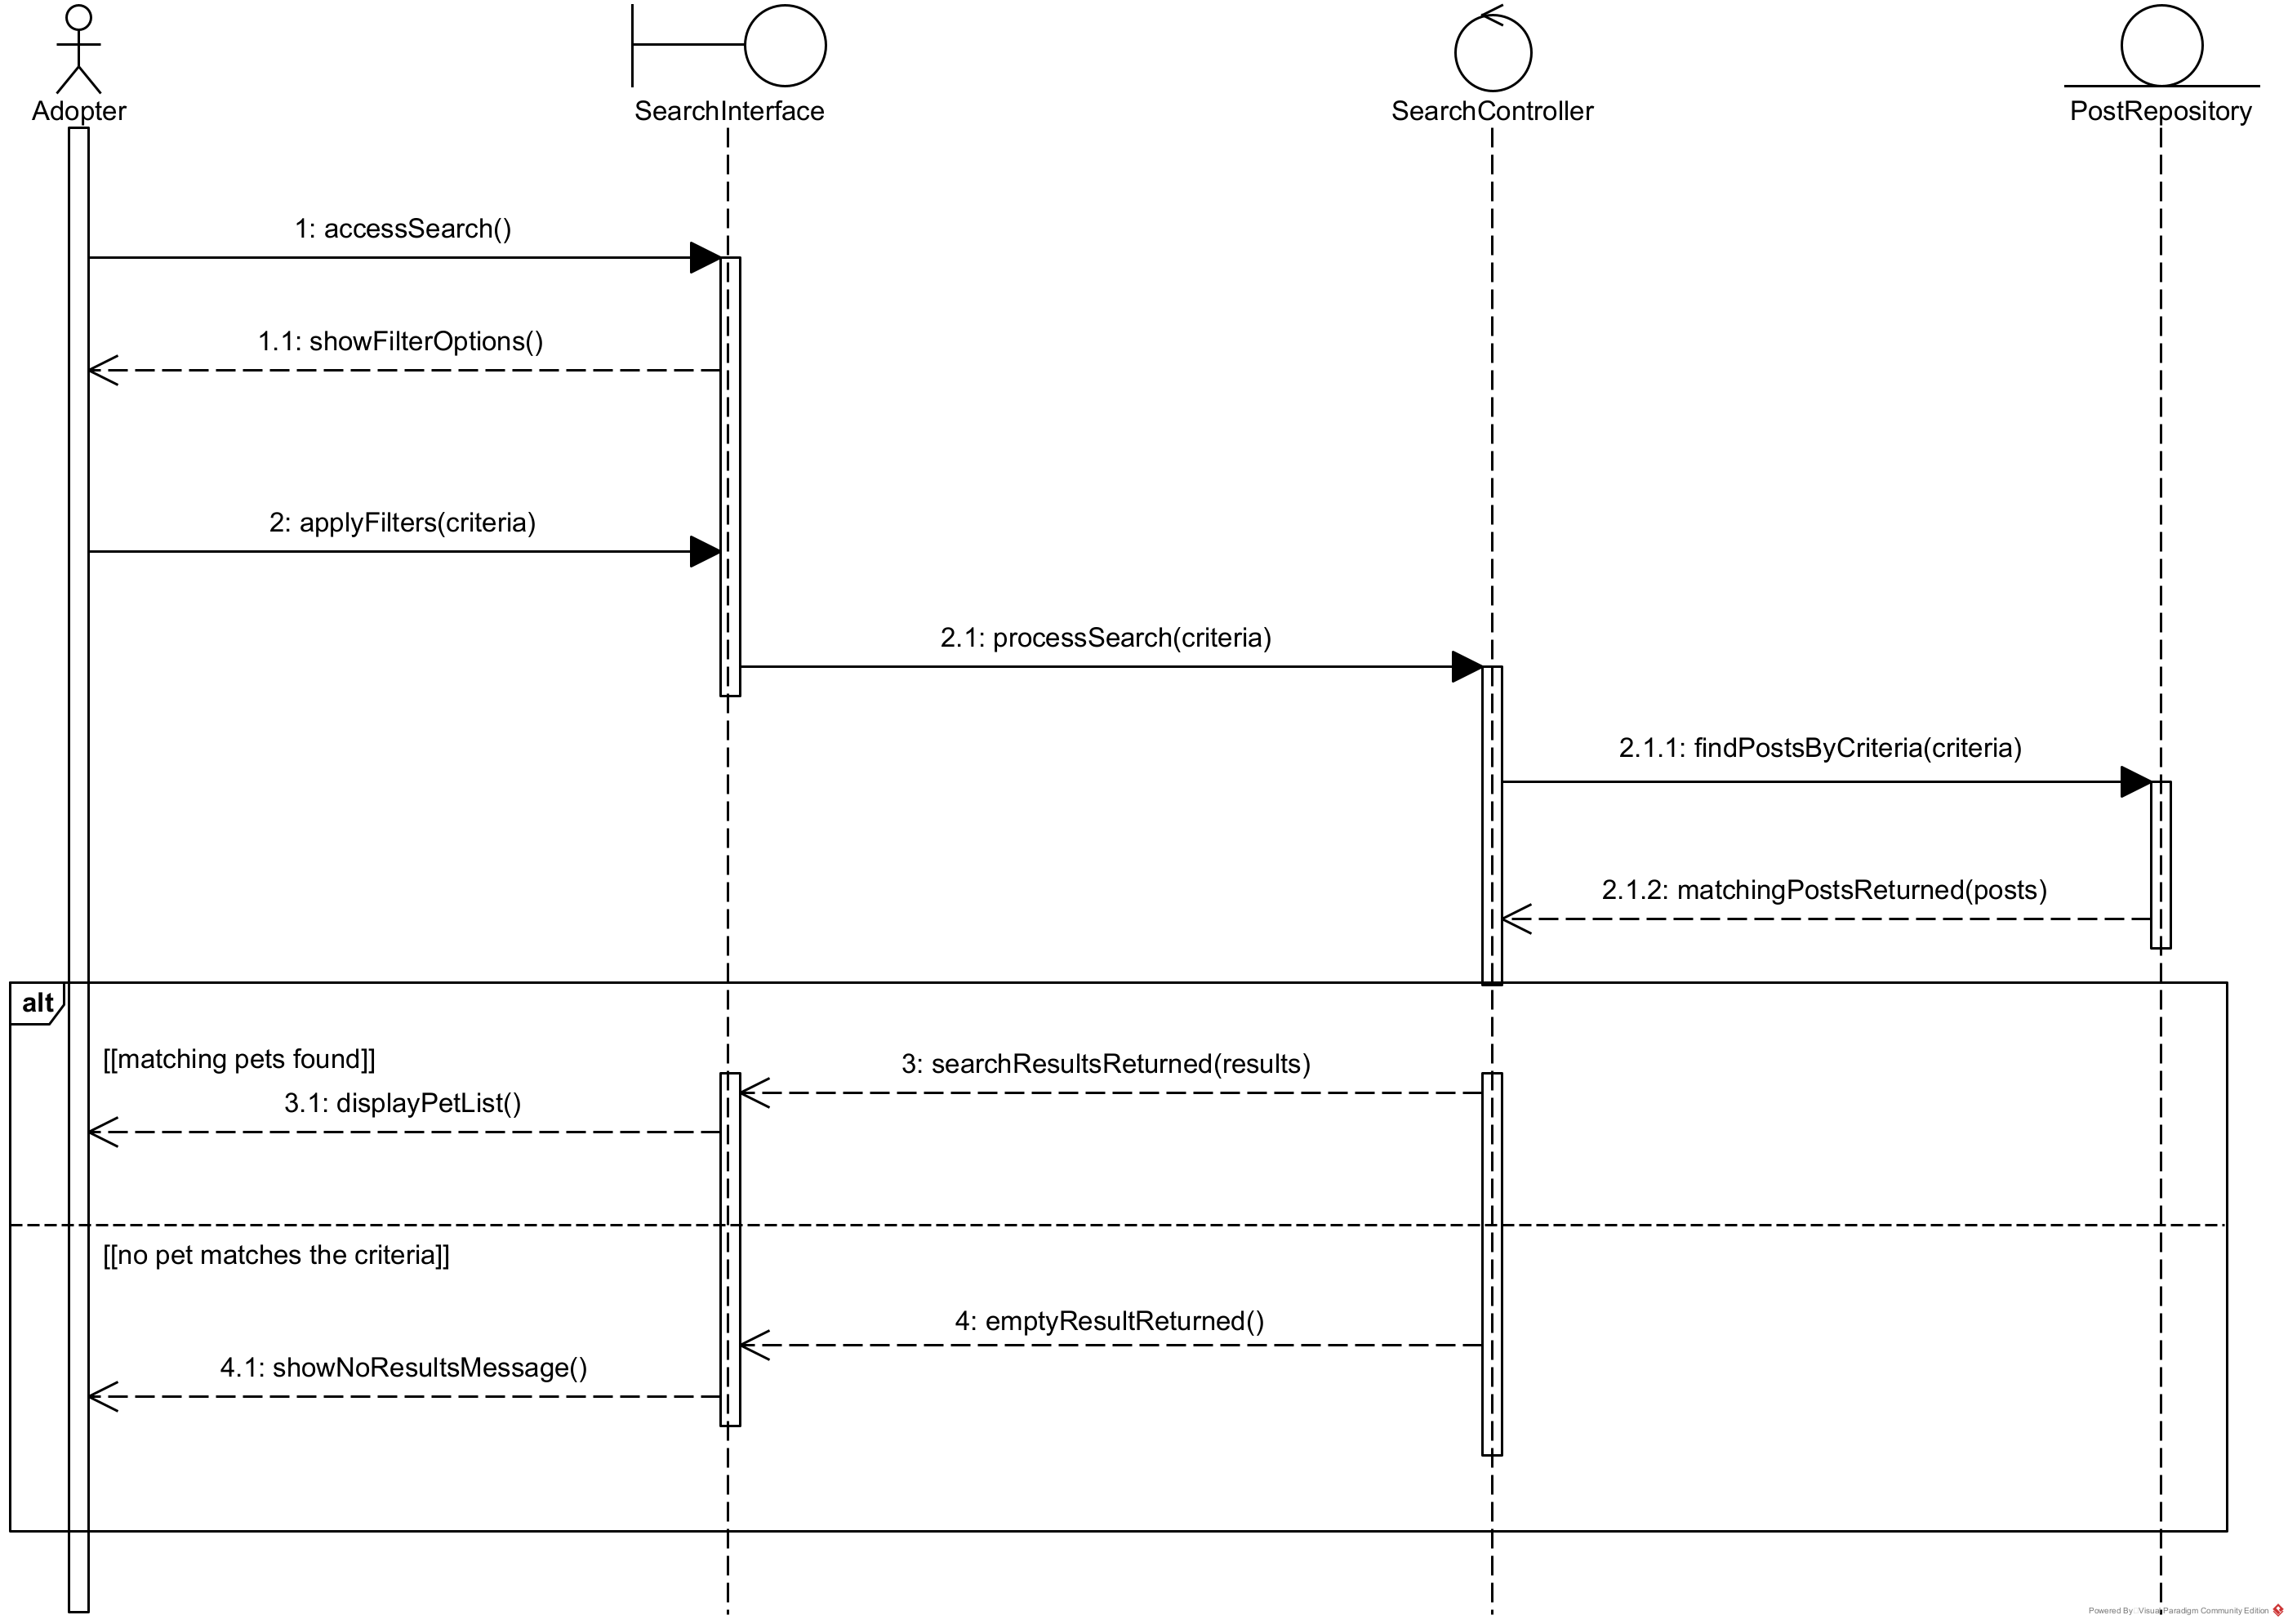
\includegraphics[width=0.72\textwidth]{figuras/DiagramaSecuencia_CU-11_MundiPets.png}
		\caption{Diagrama de secuencia del caso de uso CU-11 --- Buscar mascota disponible.}
		\label{fig:sec-cu11}
	\end{figure}

	\subsubsection{Consultar recomendaciones de cuidado (contenido real del archivo CU-12)}

	El archivo \texttt{DiagramaSecuencia\_CU-12} representa la consulta de
	recomendaciones de cuidado preventivo (relacionada con RF-10), un caso de
	uso de apoyo identificado en el diagrama de casos de uso general
	(\emph{Check care recommendations}) que no cuenta con un número CU propio
	en la especificación textual vigente de la Sección~\ref{sec:cu-detallado}.
	El controlador (\texttt{CareRecommendationController}) obtiene la
	especie, la raza y la fecha de nacimiento de la mascota; si ambos datos
	están especificados, consulta las pautas de cuidado correspondientes y las
	vacunas pendientes para generar una recomendación específica, y si falta
	alguno de los dos datos, retorna en su lugar una recomendación básica
	genérica.

	\begin{figure}[H]
		\centering
		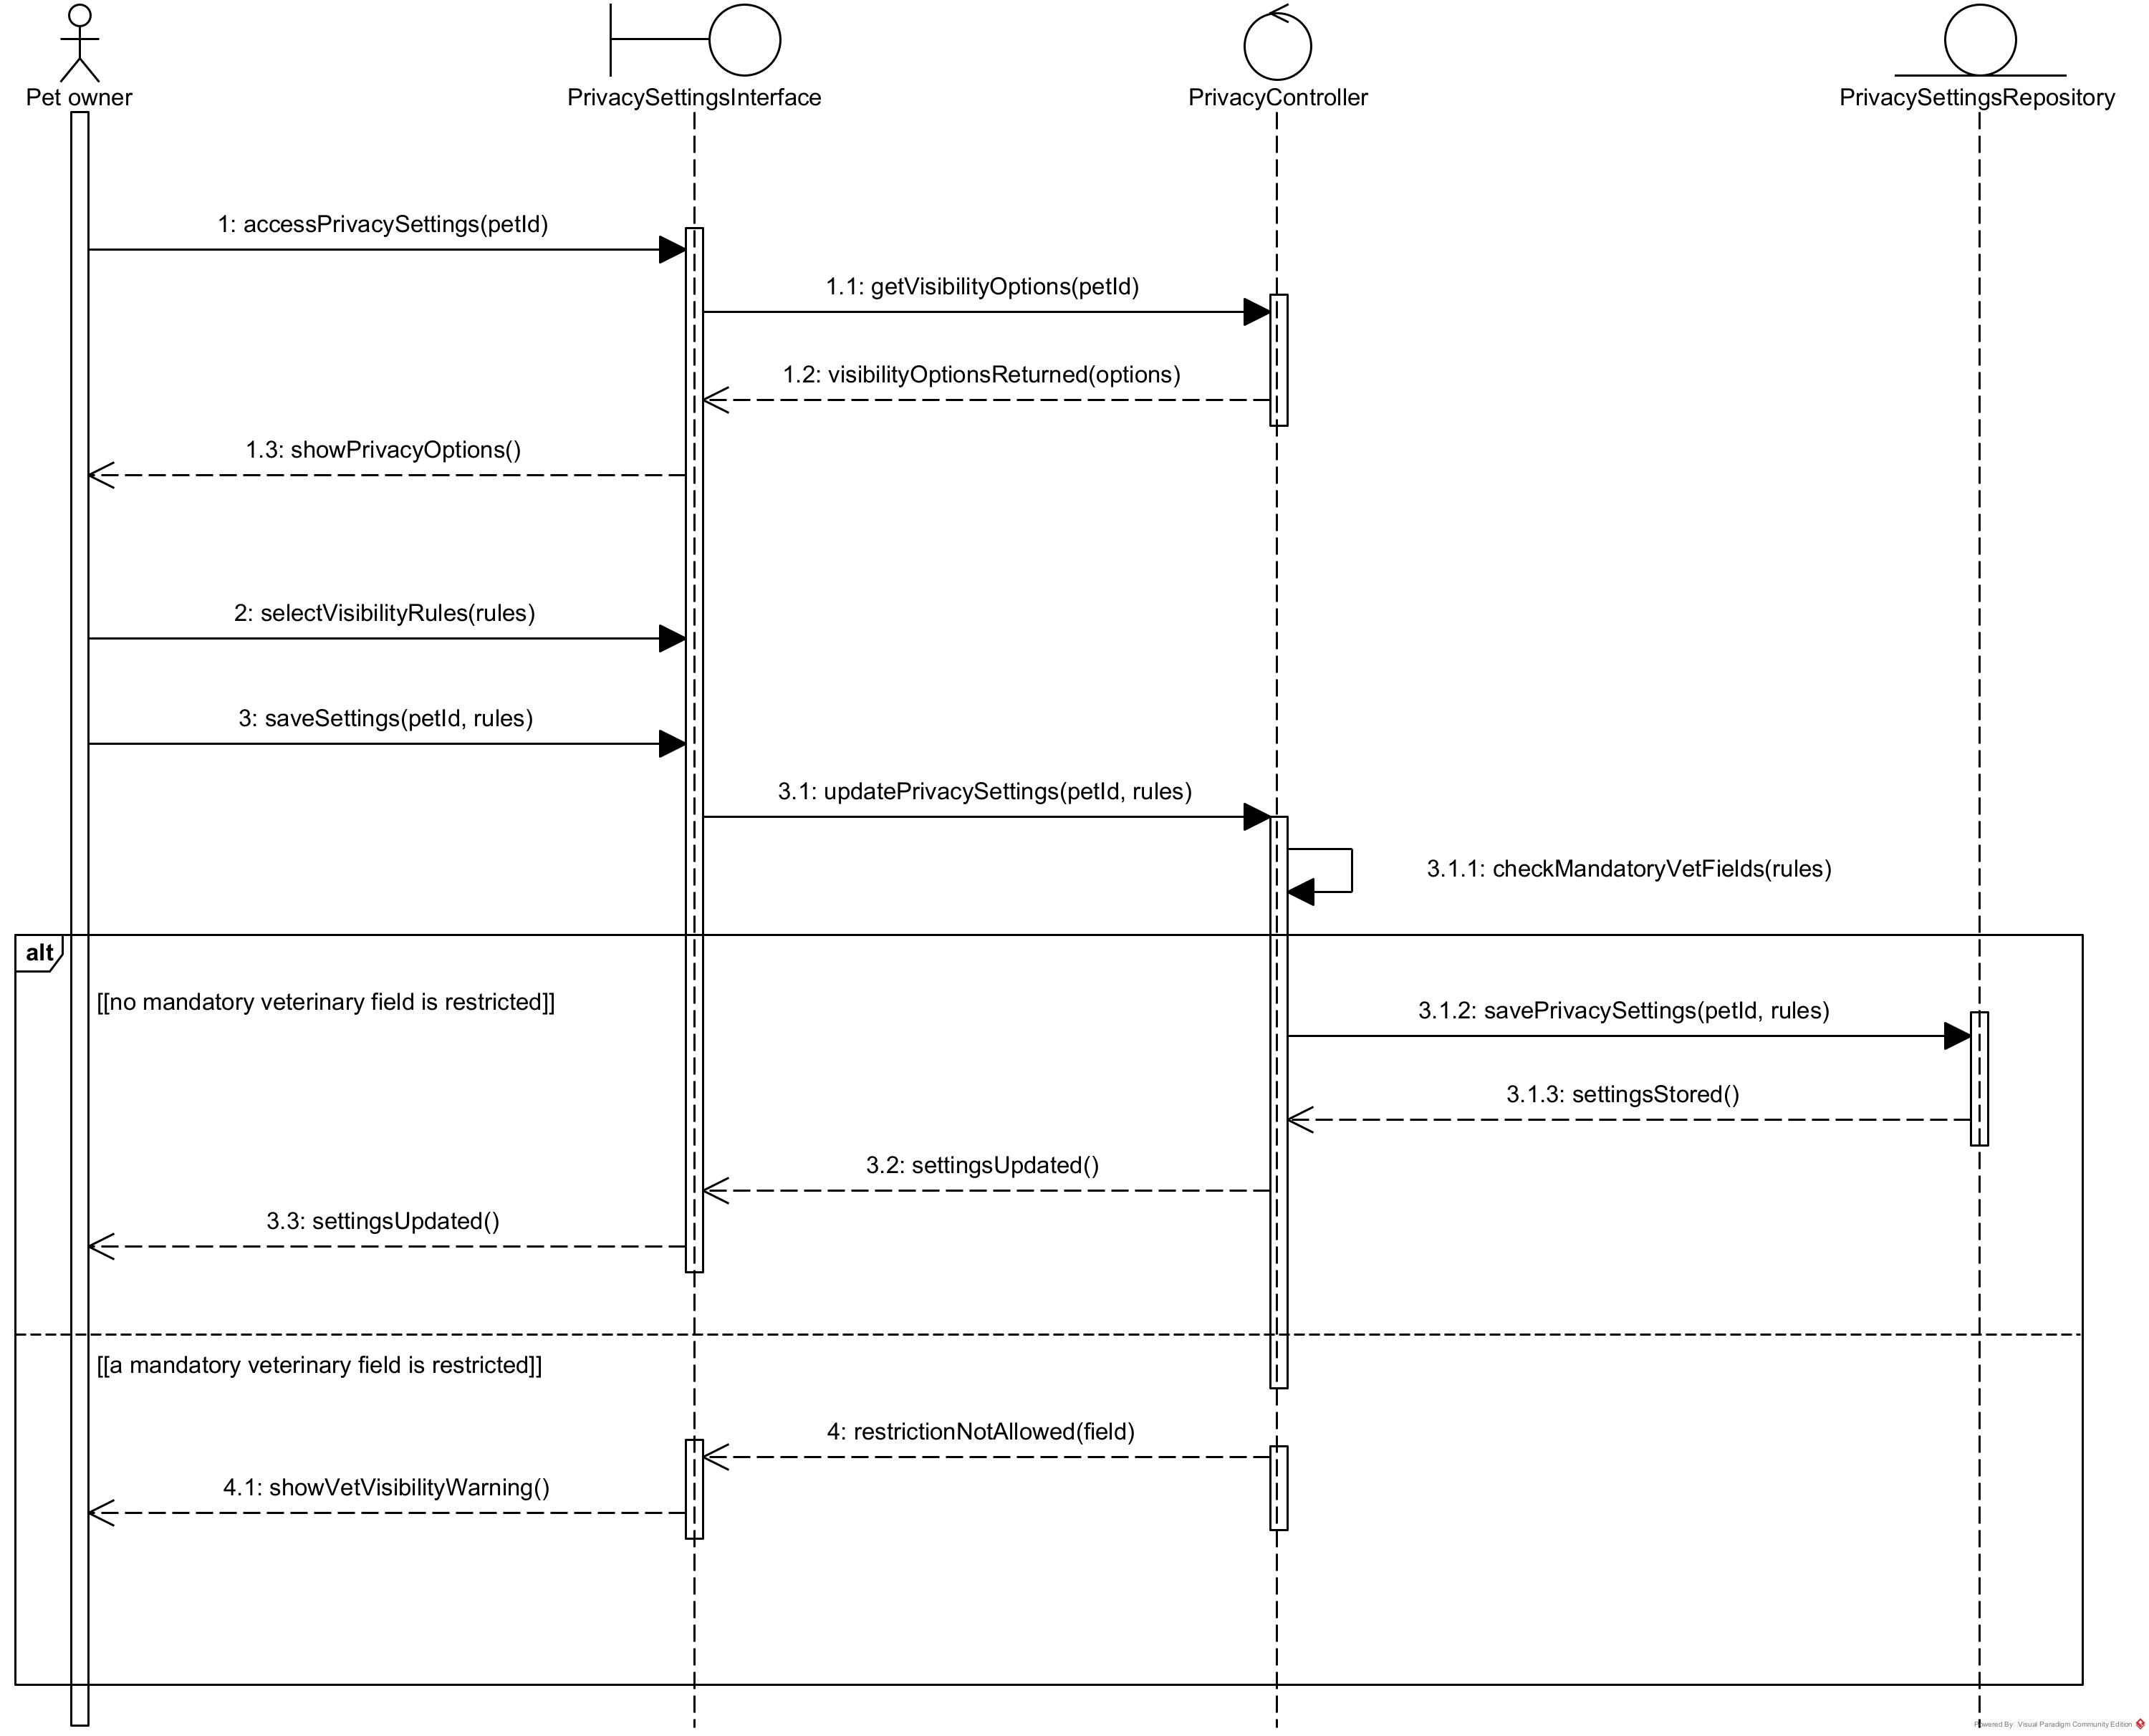
\includegraphics[width=0.72\textwidth]{figuras/DiagramaSecuencia_CU-12_MundiPets.png}
		\caption{Diagrama de secuencia --- Consultar recomendaciones de cuidado (archivo etiquetado CU-12).}
		\label{fig:sec-cu12}
	\end{figure}

	\subsubsection{Evaluar compatibilidad de cruza (contenido real del archivo CU-13)}

	El archivo \texttt{DiagramaSecuencia\_CU-13} contiene la interacción más
	compleja del sistema desde el punto de vista de la inteligencia
	artificial (especificada como CU-06 en la Sección~\ref{sec:cu-detallado};
	véase la nota de verificación al inicio de esta subsección), e integra en
	un solo diagrama tanto la evaluación de compatibilidad como la
	verificación de parentesco que la especificación textual trata por
	separado como CU-13. Tras la selección de las dos mascotas, el controlador
	(\texttt{CompatibilityController}) extrae en un ciclo el historial clínico
	de cada una y envía los datos al servicio externo de inteligencia
	artificial (\texttt{ExternalAIService}); si el resultado obtenido indica
	un puntaje de compatibilidad igual o superior a 0.85 y ausencia de
	consanguinidad, el sistema emite el informe de compatibilidad, y si detecta
	un campo faltante o consanguinidad, retorna en su lugar una alerta de
	riesgo biológico sin llegar a emitir una recomendación.

	\begin{figure}[H]
		\centering
		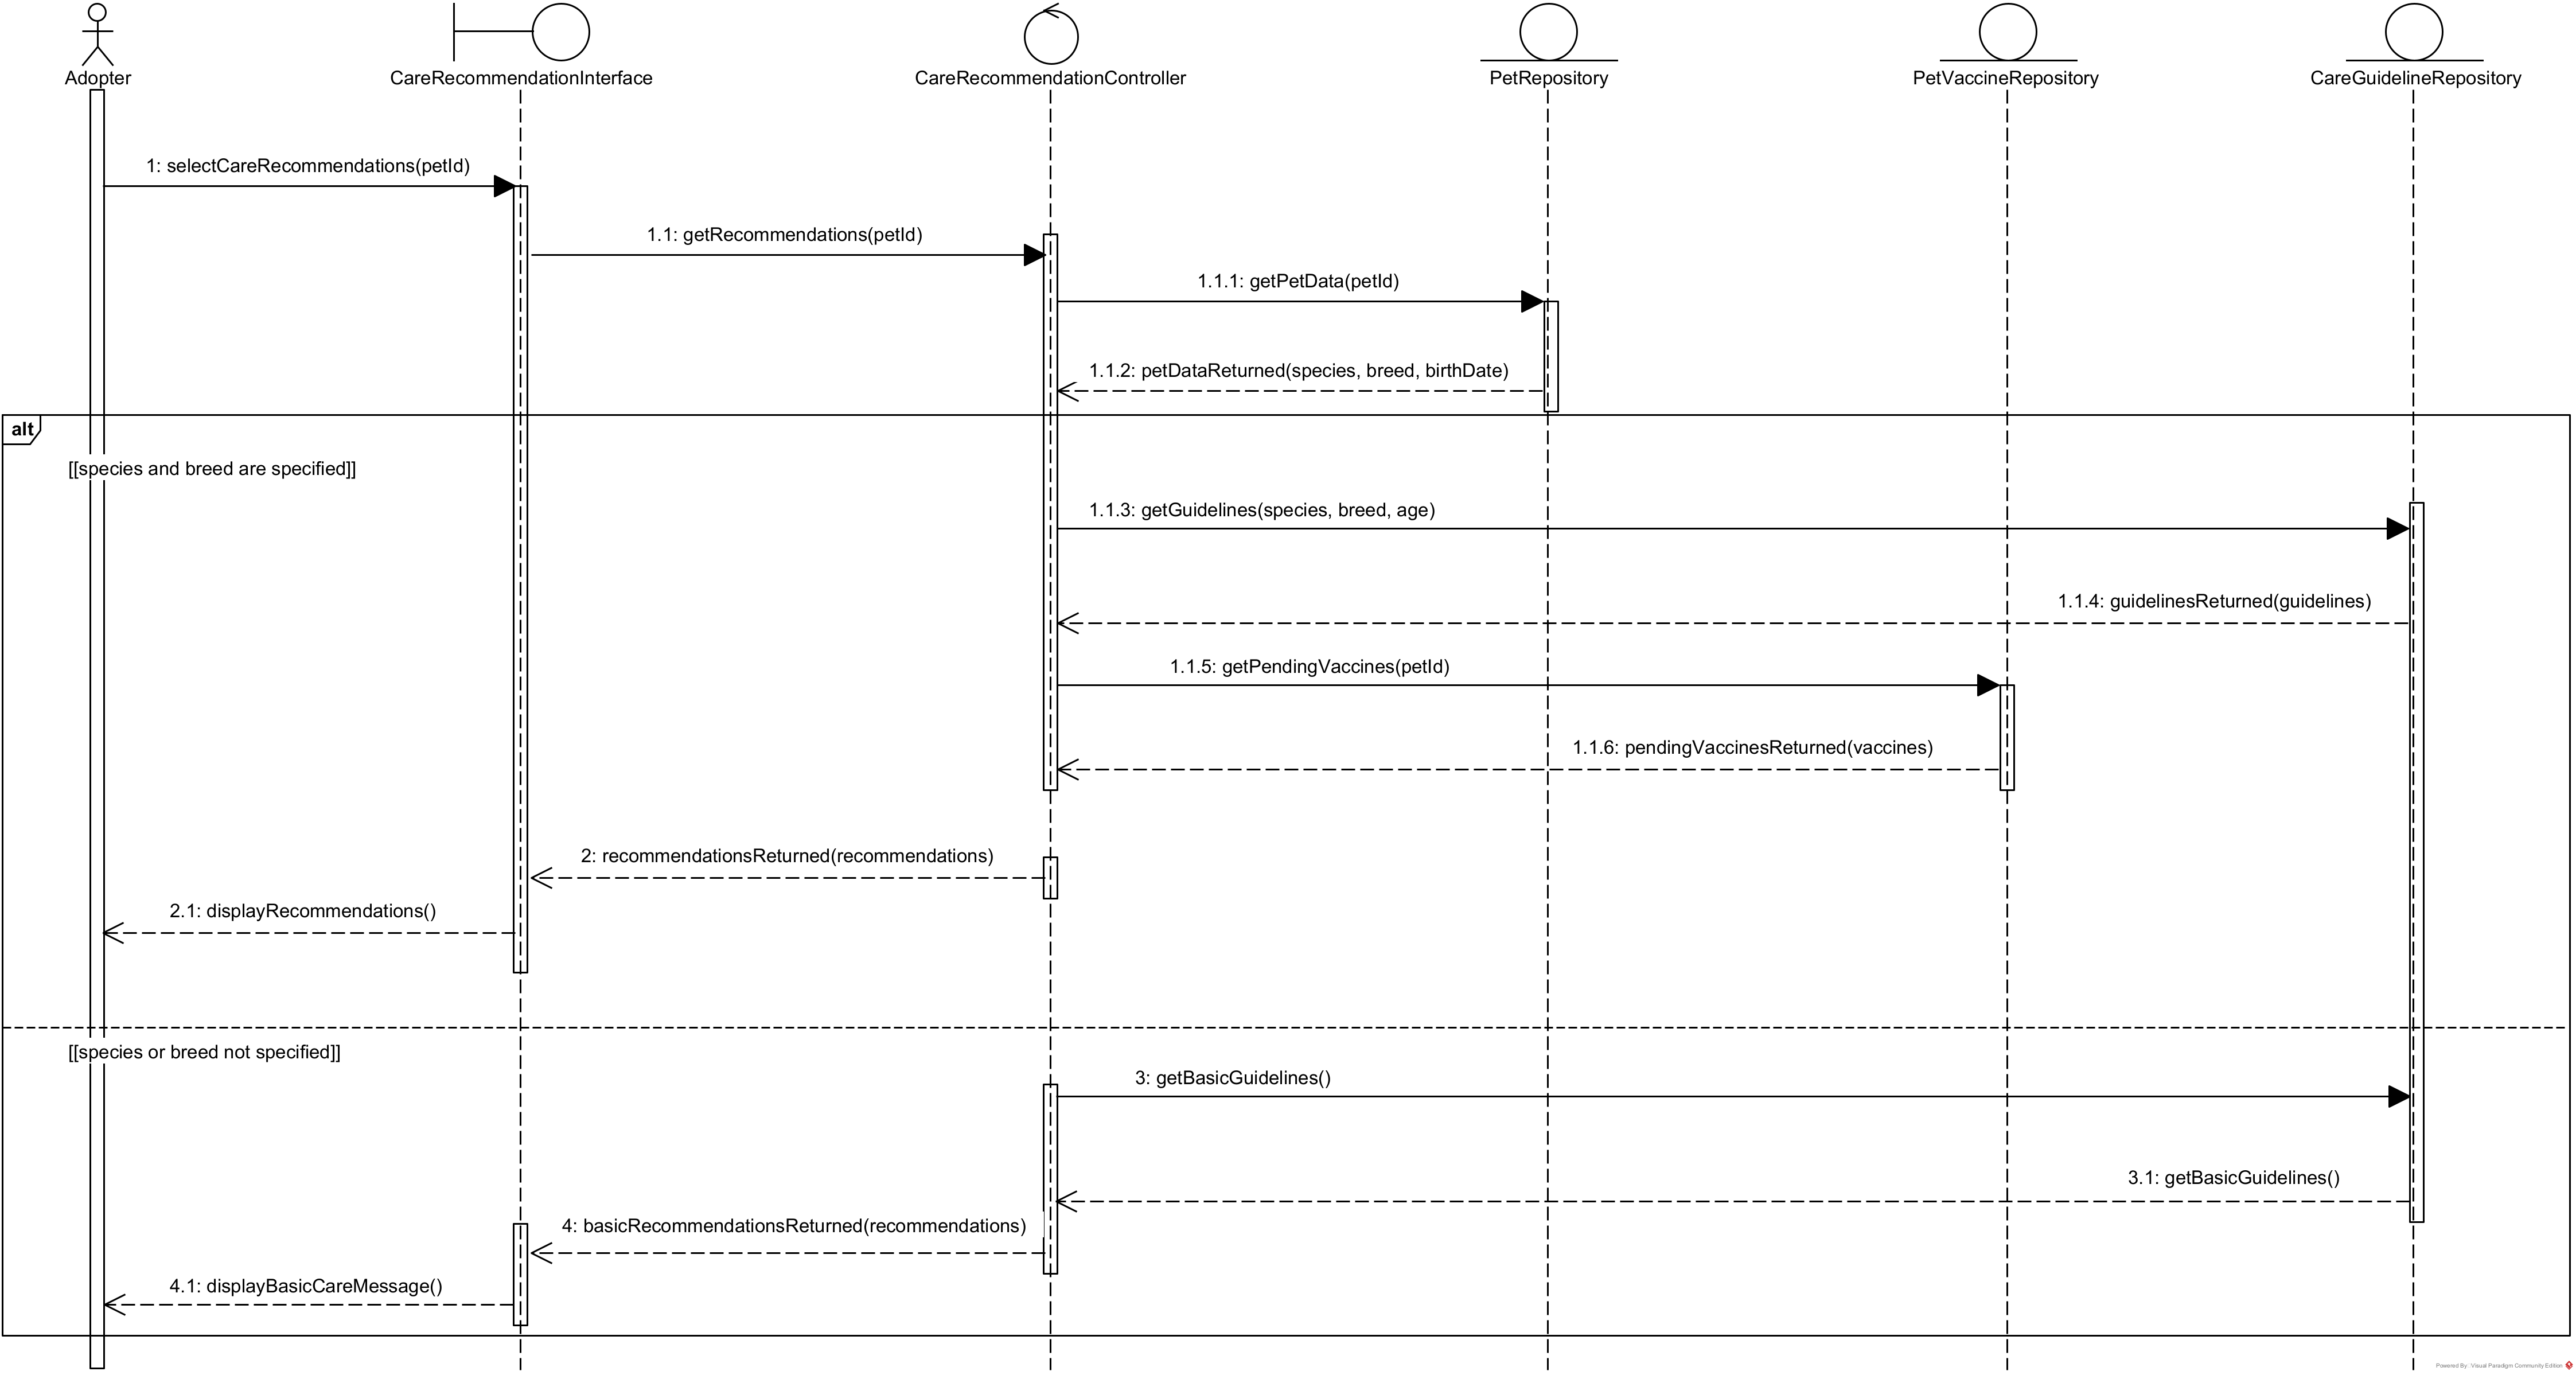
\includegraphics[width=0.72\textwidth]{figuras/DiagramaSecuencia_CU-13_MundiPets.png}
		\caption{Diagrama de secuencia --- Evaluar compatibilidad de cruza y verificación de parentesco (archivo etiquetado CU-13; corresponde a CU-06 y CU-13).}
		\label{fig:sec-cu13}
	\end{figure}

	\subsection{Diagramas de actividad}
	\label{sec:actividad}

	Los diagramas de actividad complementan a los diagramas de secuencia al
	representar el flujo de control y las decisiones lógicas dentro de cada caso
	de uso, incluyendo bifurcaciones, uniones y flujos alternos que no se
	aprecian con la misma claridad en una vista basada en intercambio de
	mensajes. A continuación se presentan los trece diagramas completos (CU-01 a
	CU-13), organizados por carriles entre el actor y el sistema. El mismo
	desajuste de numeración documentado en la nota de verificación de la
	Sección~\ref{sec:secuencia} para los archivos de secuencia se repite de
	forma idéntica en los archivos de actividad: los identificados como CU-06,
	CU-07, CU-12 y CU-13 no corresponden al caso de uso que su nombre indica,
	sino respectivamente a la configuración de privacidad médica (CU-12), la
	gestión de una solicitud de adopción, la consulta de recomendaciones de
	cuidado, y la evaluación de compatibilidad de cruza con verificación de
	parentesco integradas (CU-06 y CU-13).

	\subsubsection{Registrar mascota (CU-01)}

	El diagrama de actividad de CU-01 muestra el flujo completo desde que el
	propietario selecciona \enquote{Register pet} hasta la confirmación del
	perfil. Tras adjuntar los datos y la fotografía, la rama de decisión
	central (\emph{Data valid?}) evalúa si los campos obligatorios están
	completos; en caso negativo, el flujo retorna al formulario mostrando de
	nuevo la pantalla de registro. Solo cuando los datos son válidos el flujo
	continúa hacia \emph{Register pet}, \emph{Validate photos} --- la
	validación de imágenes exigida por RF-17 --- y finalmente el almacenamiento
	del registro.

	\begin{figure}[H]
		\centering
		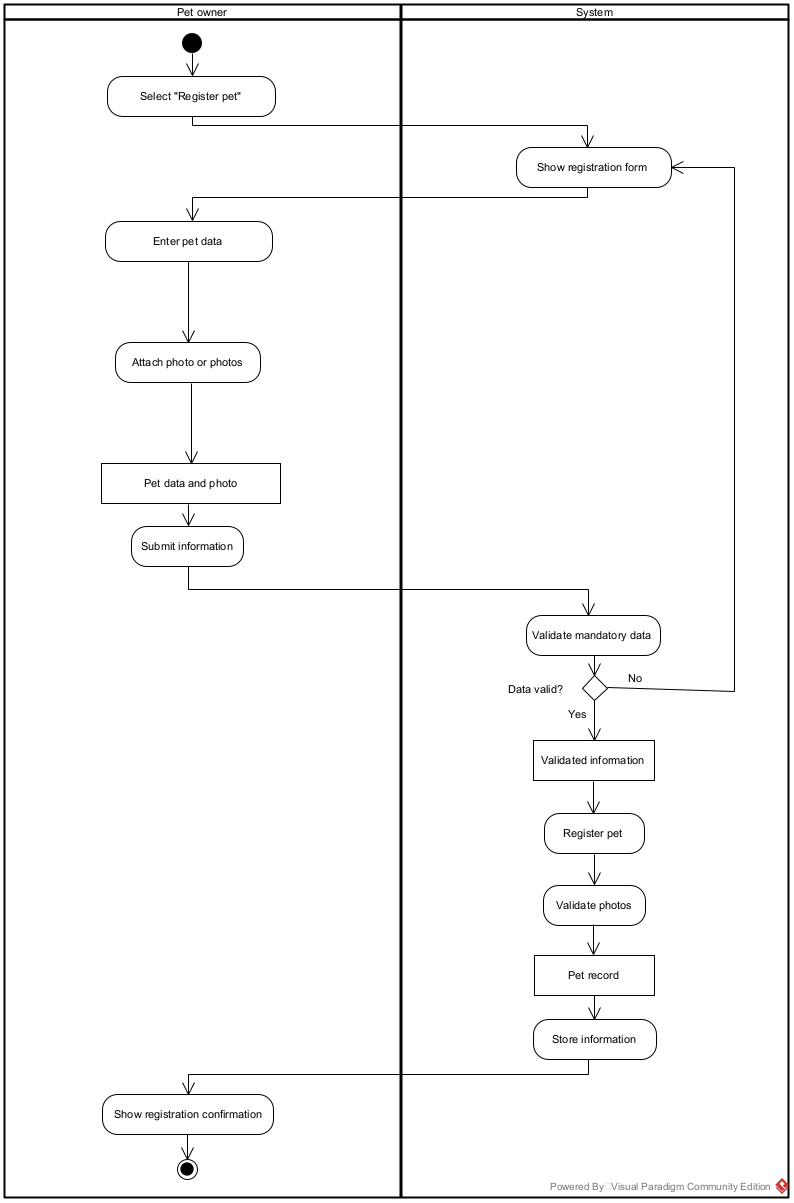
\includegraphics[width=0.66\textwidth]{figuras/DiagramaActividades_CU-01_MundiPets.png}
		\caption{Diagrama de actividad del caso de uso CU-01 --- Registrar mascota.}
		\label{fig:act-cu01}
	\end{figure}

	\subsubsection{Registrar historial médico y antecedentes genéticos (CU-02)}

	Este diagrama detalla el flujo de registro del historial médico de una
	mascota (RF-02): el propietario completa y envía el formulario, y el
	sistema verifica la completitud de los datos antes de registrar la
	información o de retornar un mensaje de error específico si algún campo
	obligatorio falta. El diagrama no distingue una bifurcación de actor entre
	propietario y veterinaria ni representa de forma explícita la trazabilidad
	de cepa, lote y aplicador de RF-24; ambos aspectos se gestionan mediante el
	estado de verificación de documentos médicos (Sección~\ref{sec:estados}) y
	el modelo de clases, no como ramas visibles de esta actividad.

	\begin{figure}[H]
		\centering
		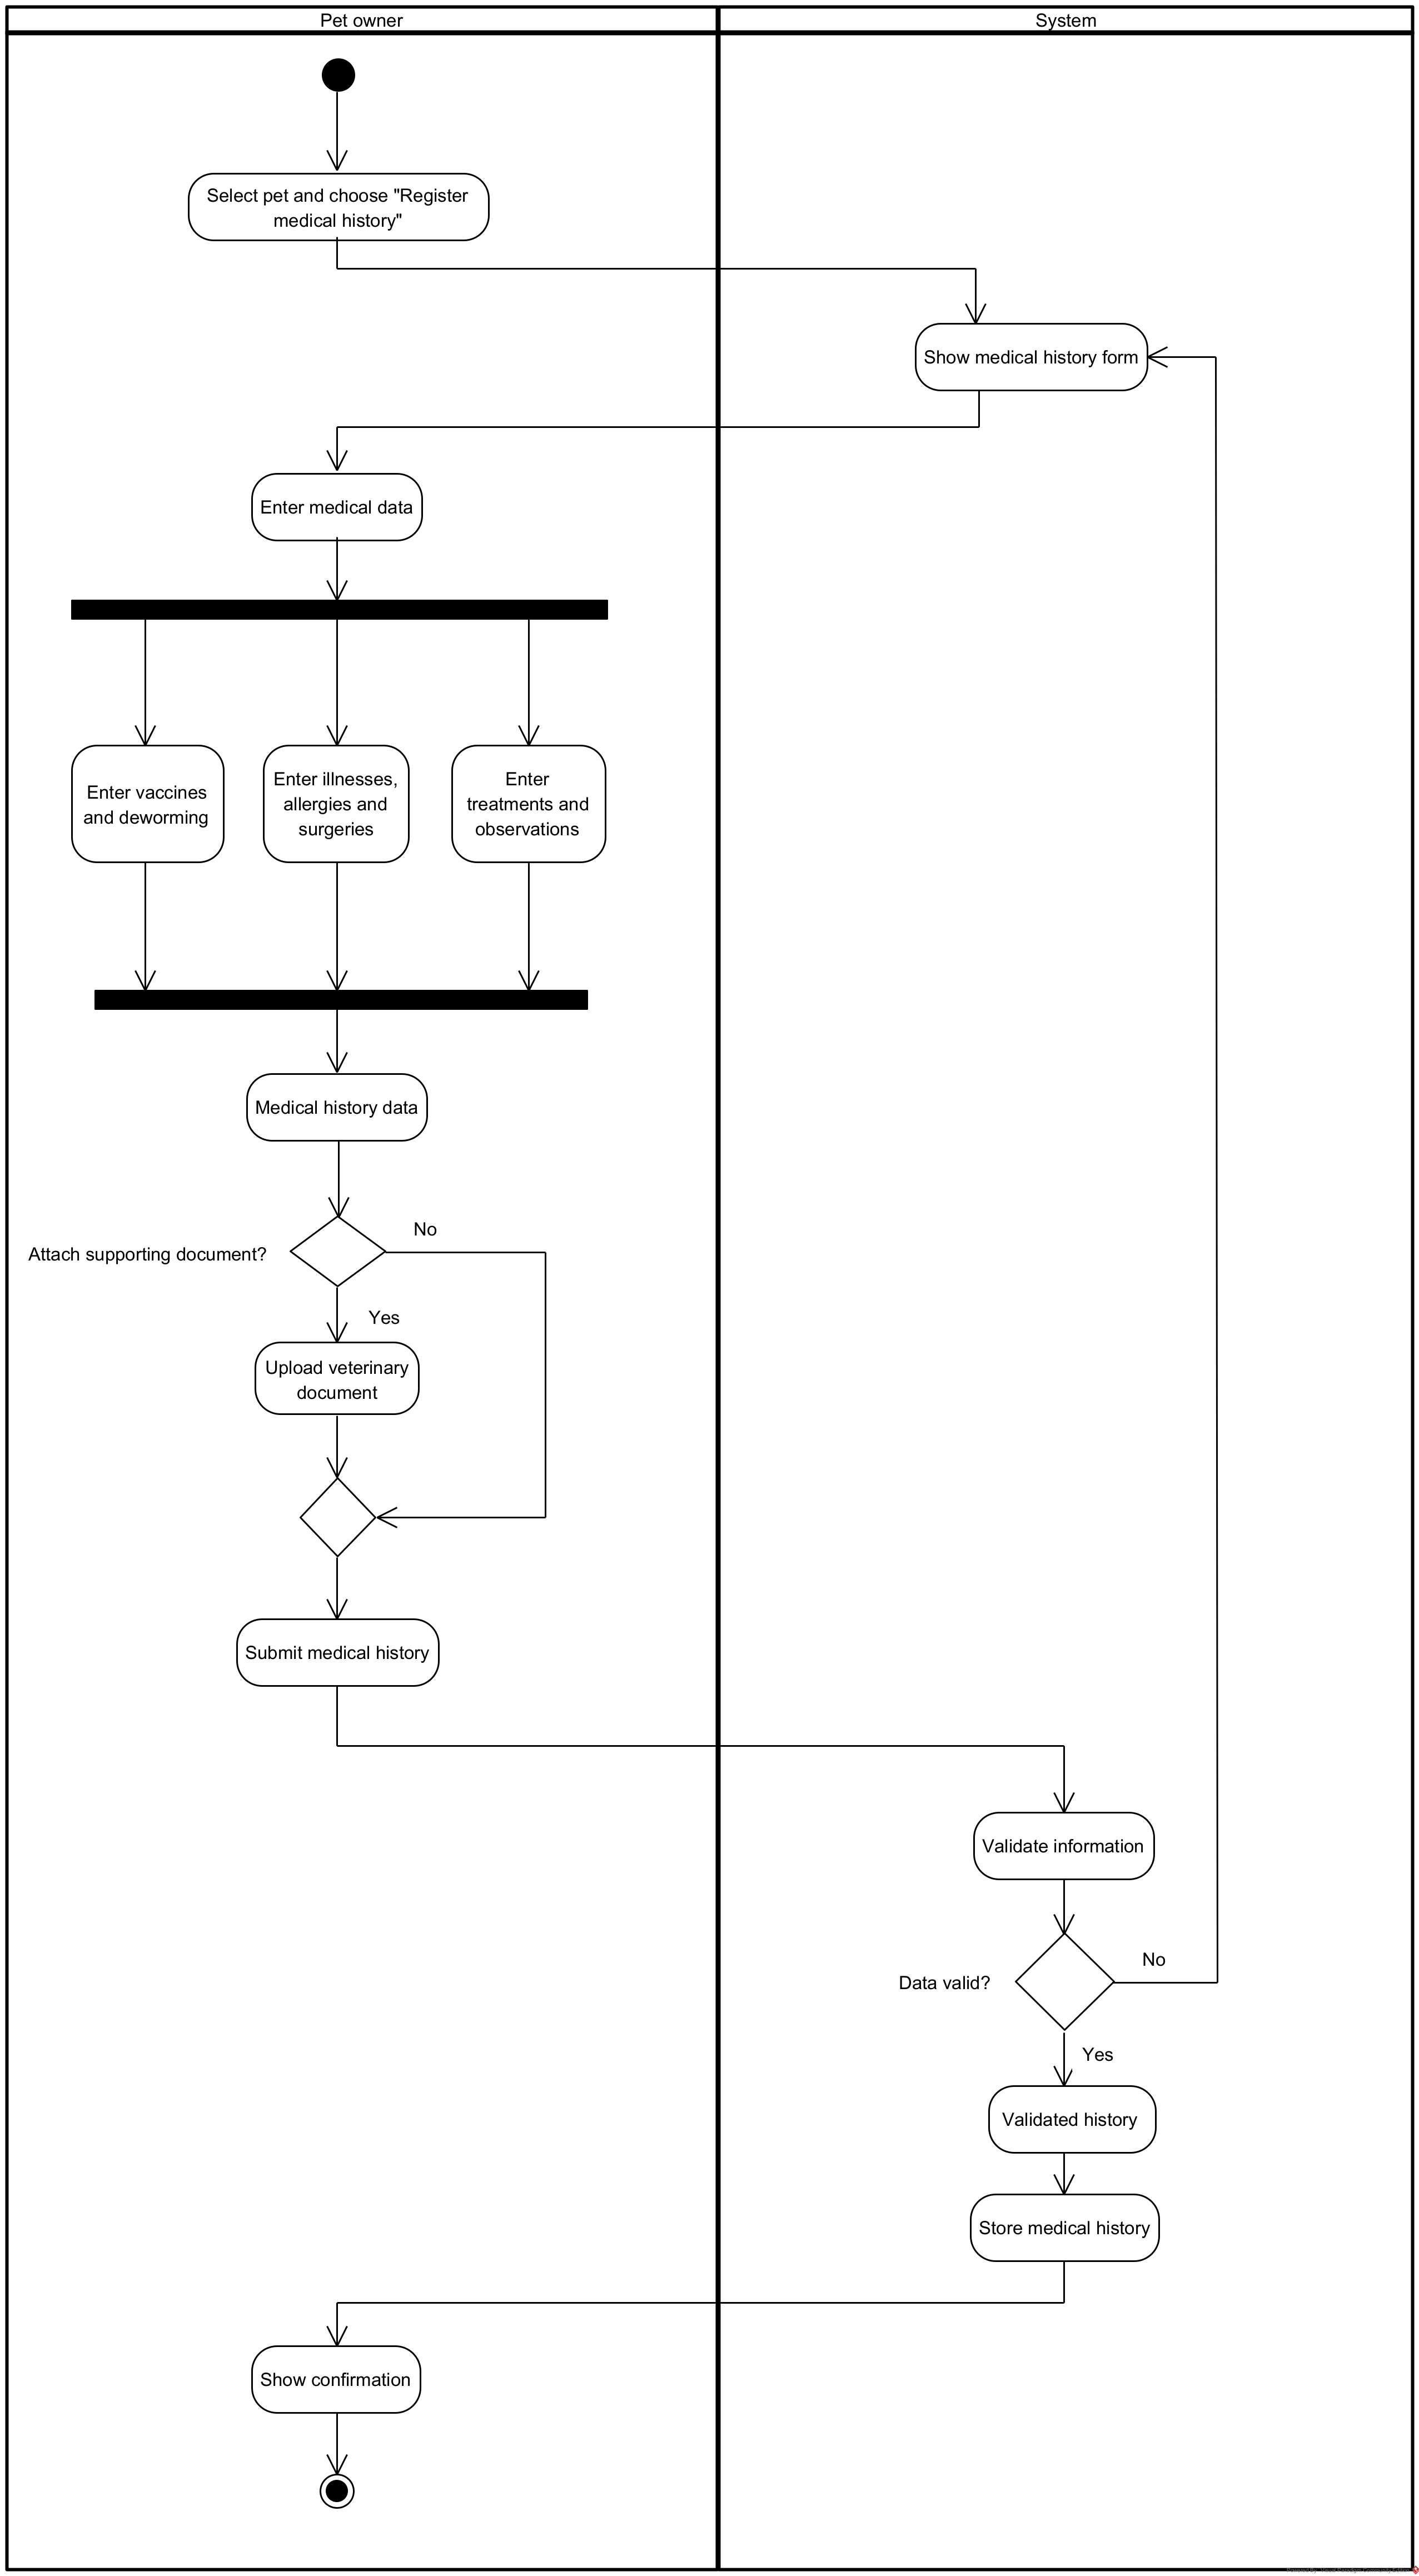
\includegraphics[width=0.56\textwidth]{figuras/DiagramaActividades_CU-02_MundiPets.png}
		\caption{Diagrama de actividad del caso de uso CU-02 --- Registrar historial médico y antecedentes genéticos.}
		\label{fig:act-cu02}
	\end{figure}

	\subsubsection{Cargar documento veterinario y carnet de vacunación (CU-03)}

	El diagrama de actividad de CU-03 representa el flujo de carga de
	documentos veterinarios (RF-14). Tras adjuntar el archivo, el sistema
	valida su formato y tamaño; si la validación falla, retorna un mensaje de
	rechazo con el motivo, y si es exitosa, almacena el archivo en el servicio
	externo y registra sus metadatos, dejando el documento disponible de
	inmediato para consulta, aunque su validación profesional --- en el flujo
	de CU-09 --- queda pendiente hasta la revisión de una veterinaria
	autorizada.

	\begin{figure}[H]
		\centering
		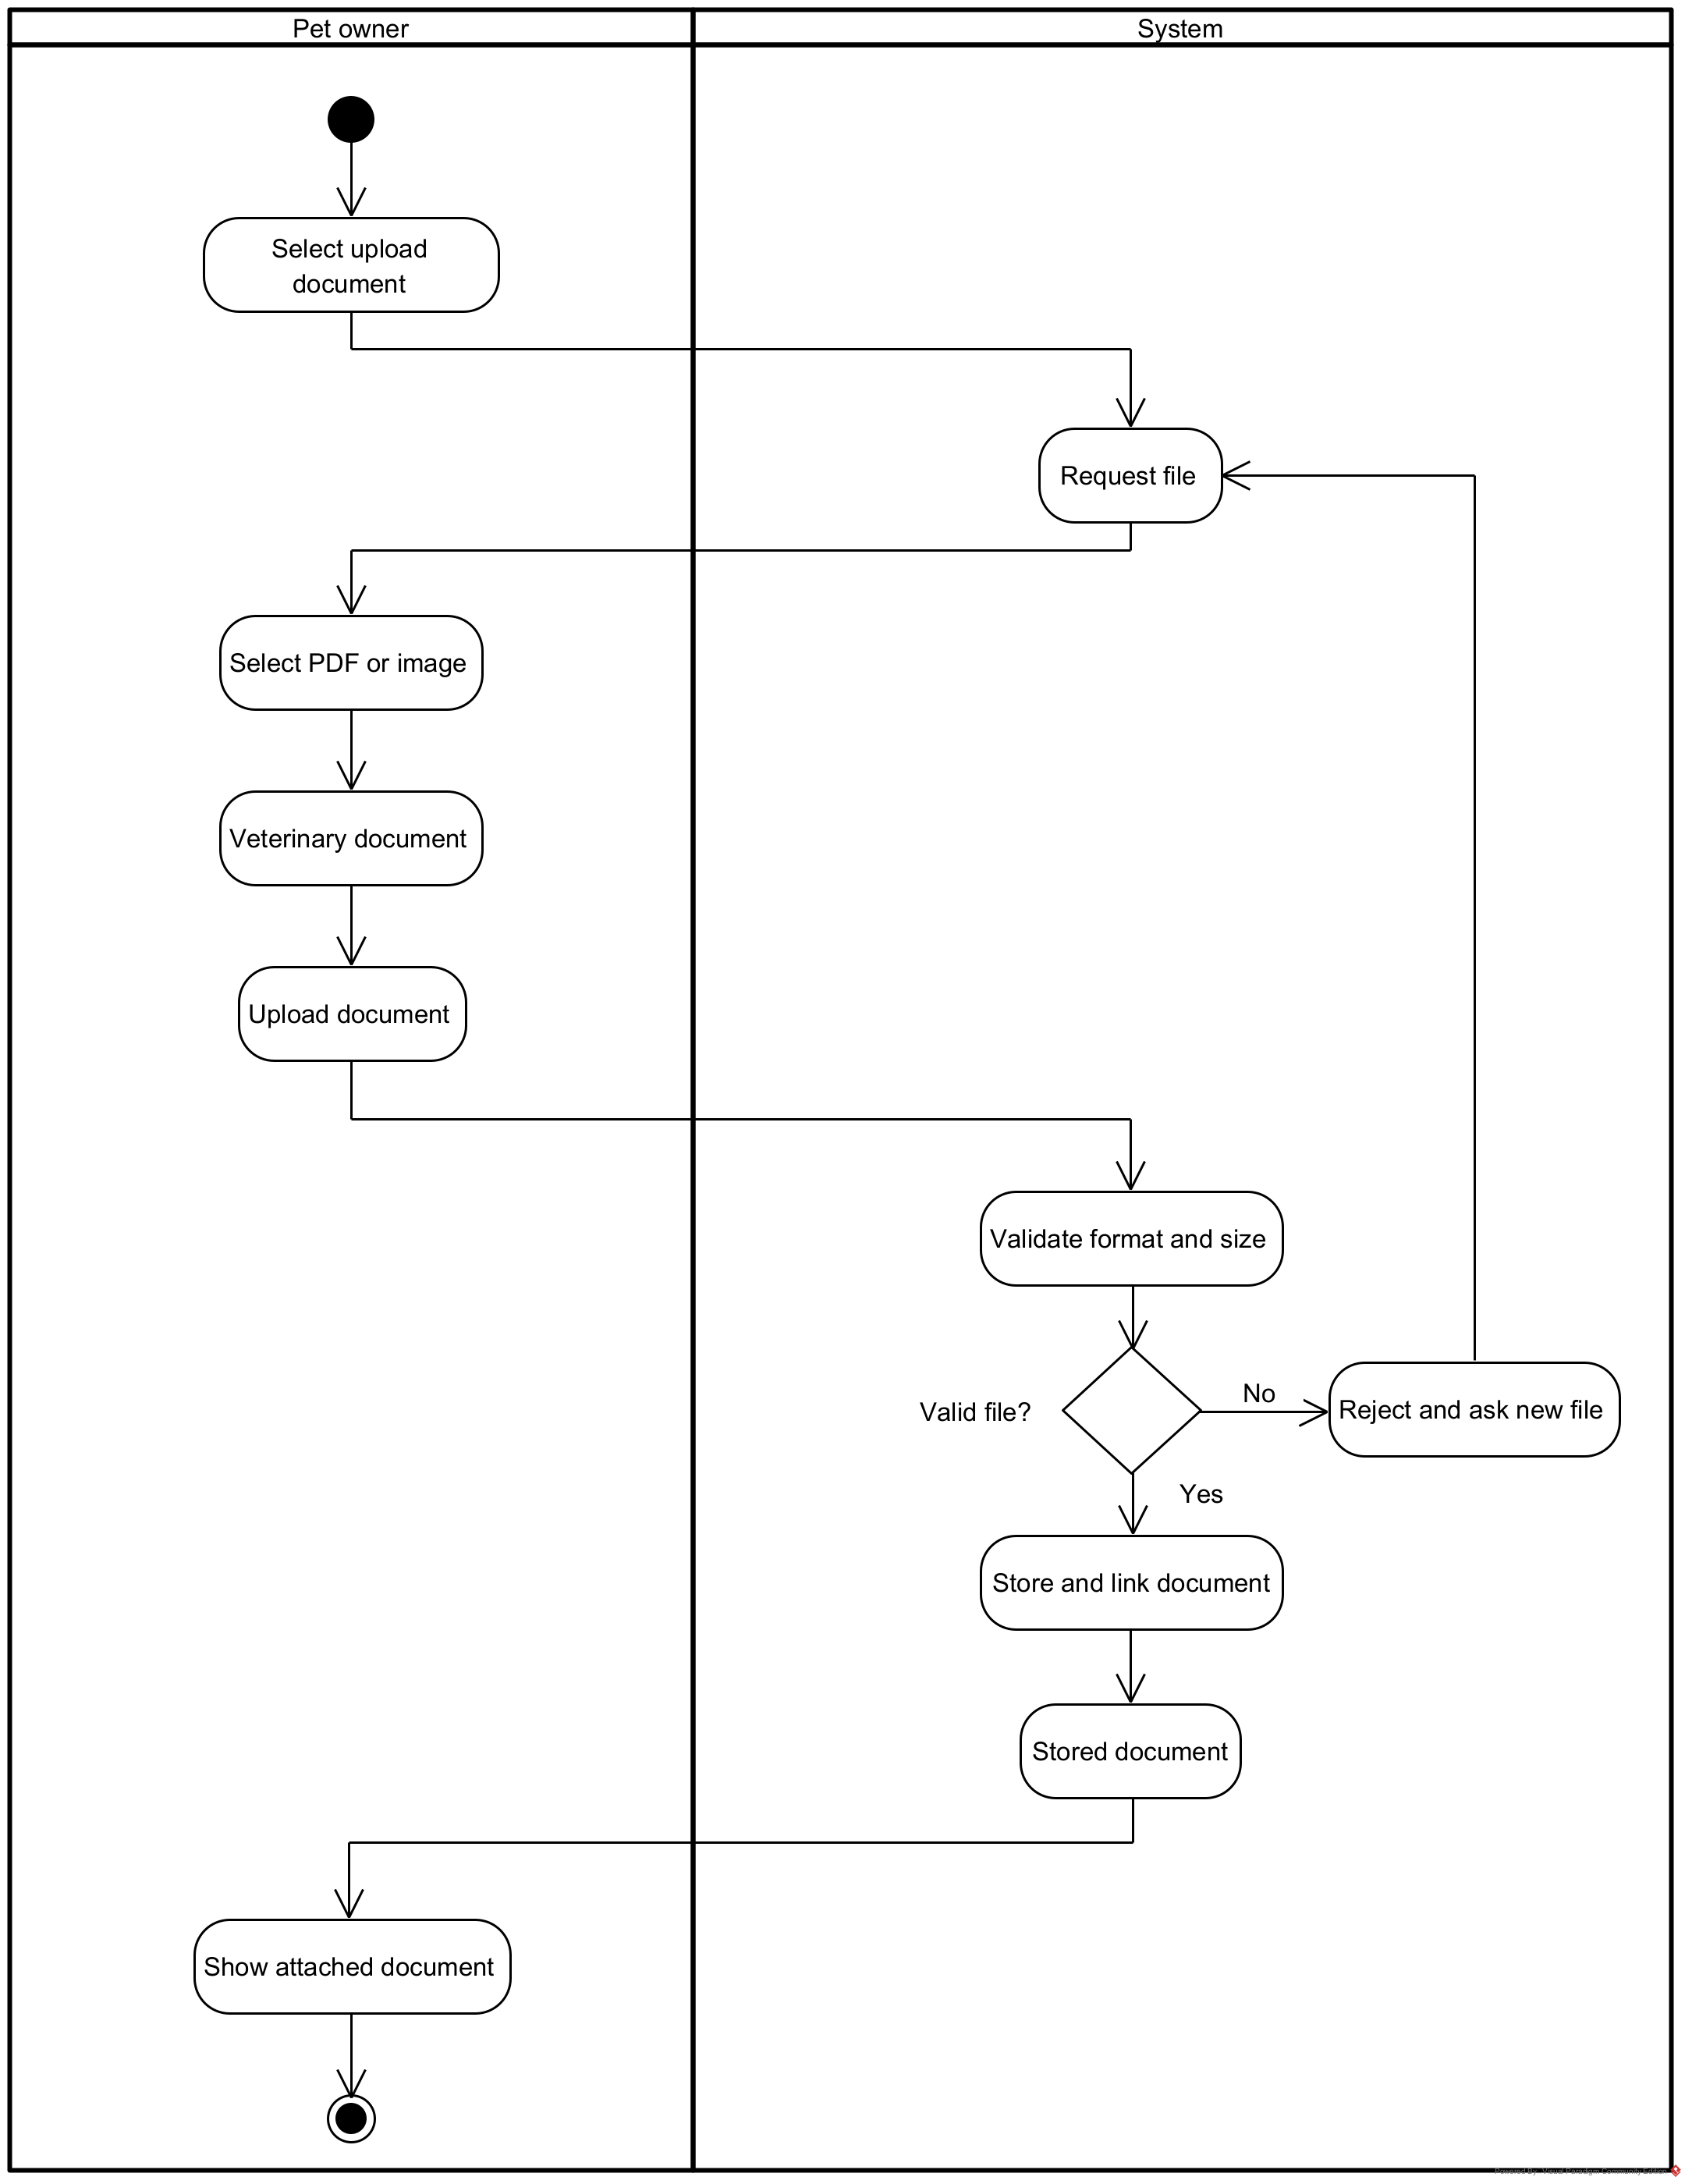
\includegraphics[width=0.77\textwidth]{figuras/DiagramaActividades_CU-03_MundiPets.png}
		\caption{Diagrama de actividad del caso de uso CU-03 --- Cargar documento veterinario y carnet de vacunación.}
		\label{fig:act-cu03}
	\end{figure}

	\subsubsection{Publicar mascota en adopción (CU-04)}

	Este diagrama expone el flujo de publicación para adopción (RF-13),
	incluyendo la bifurcación que determina si la mascota ya cuenta con una
	publicación activa. Si existe una publicación previa, el flujo ofrece al
	propietario actualizarla en lugar de crear un duplicado; si no existe, el
	sistema procede directamente a almacenar y publicar la nueva mascota en el
	listado de adopciones disponibles.

	\begin{figure}[H]
		\centering
		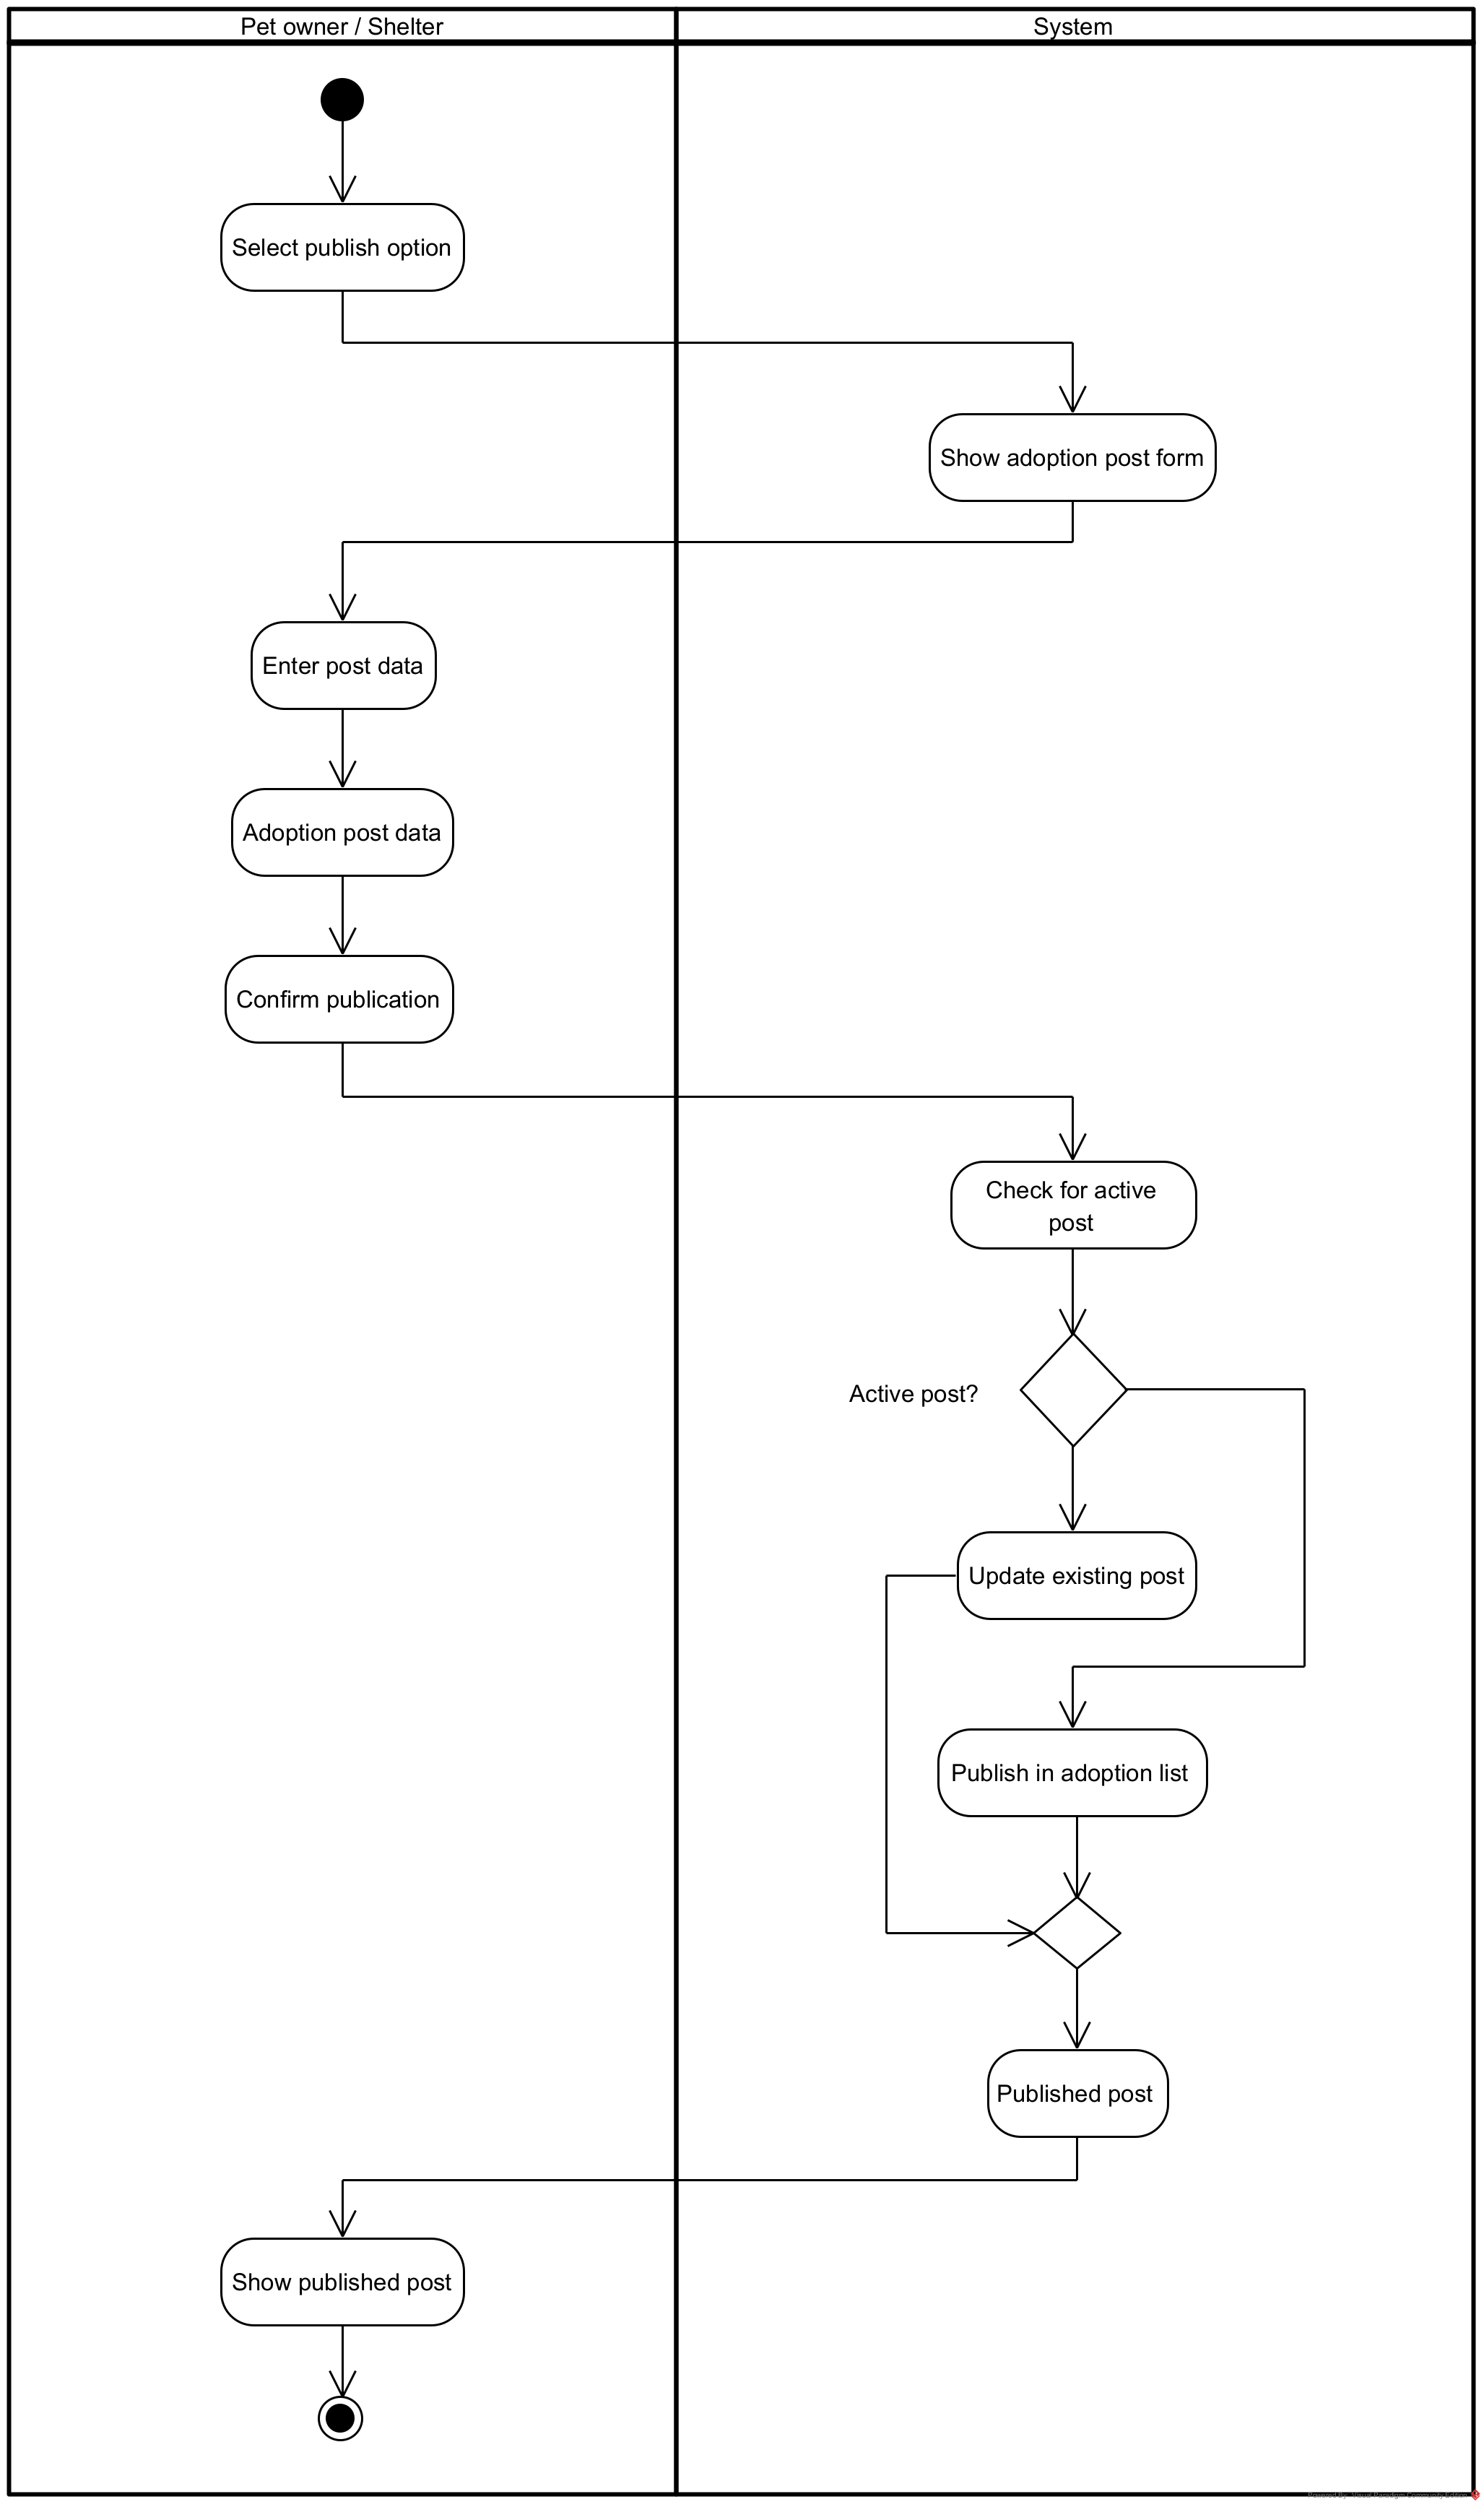
\includegraphics[width=0.60\textwidth]{figuras/DiagramaActividades_CU-04_MundiPets.png}
		\caption{Diagrama de actividad del caso de uso CU-04 --- Publicar mascota en adopción.}
		\label{fig:act-cu04}
	\end{figure}

	\subsubsection{Publicar mascota para cruza (CU-05)}

	Este diagrama representa específicamente el flujo de publicación para
	cruza responsable (RF-08, RF-13). La bifurcación central del diagrama
	comprueba si la mascota cuenta con antecedentes genéticos registrados; si
	no los tiene, el flujo dirige al propietario hacia el formulario de
	antecedentes genéticos antes de permitir continuar, garantizando que
	ninguna mascota quede publicada para cruza sin la información mínima que
	exige RF-16. La gestión posterior de la solicitud recibida --- aceptación
	o rechazo por el propietario receptor --- y la regla de negocio de RF-27
	sobre solicitudes repetitivas se representan en el flujo de gestión de
	solicitud de adopción (CU-07, según el contenido real de su archivo), cuyo
	patrón es análogo para cruza, y en la máquina de estados de la
	Sección~\ref{sec:estados}.

	\begin{figure}[H]
		\centering
		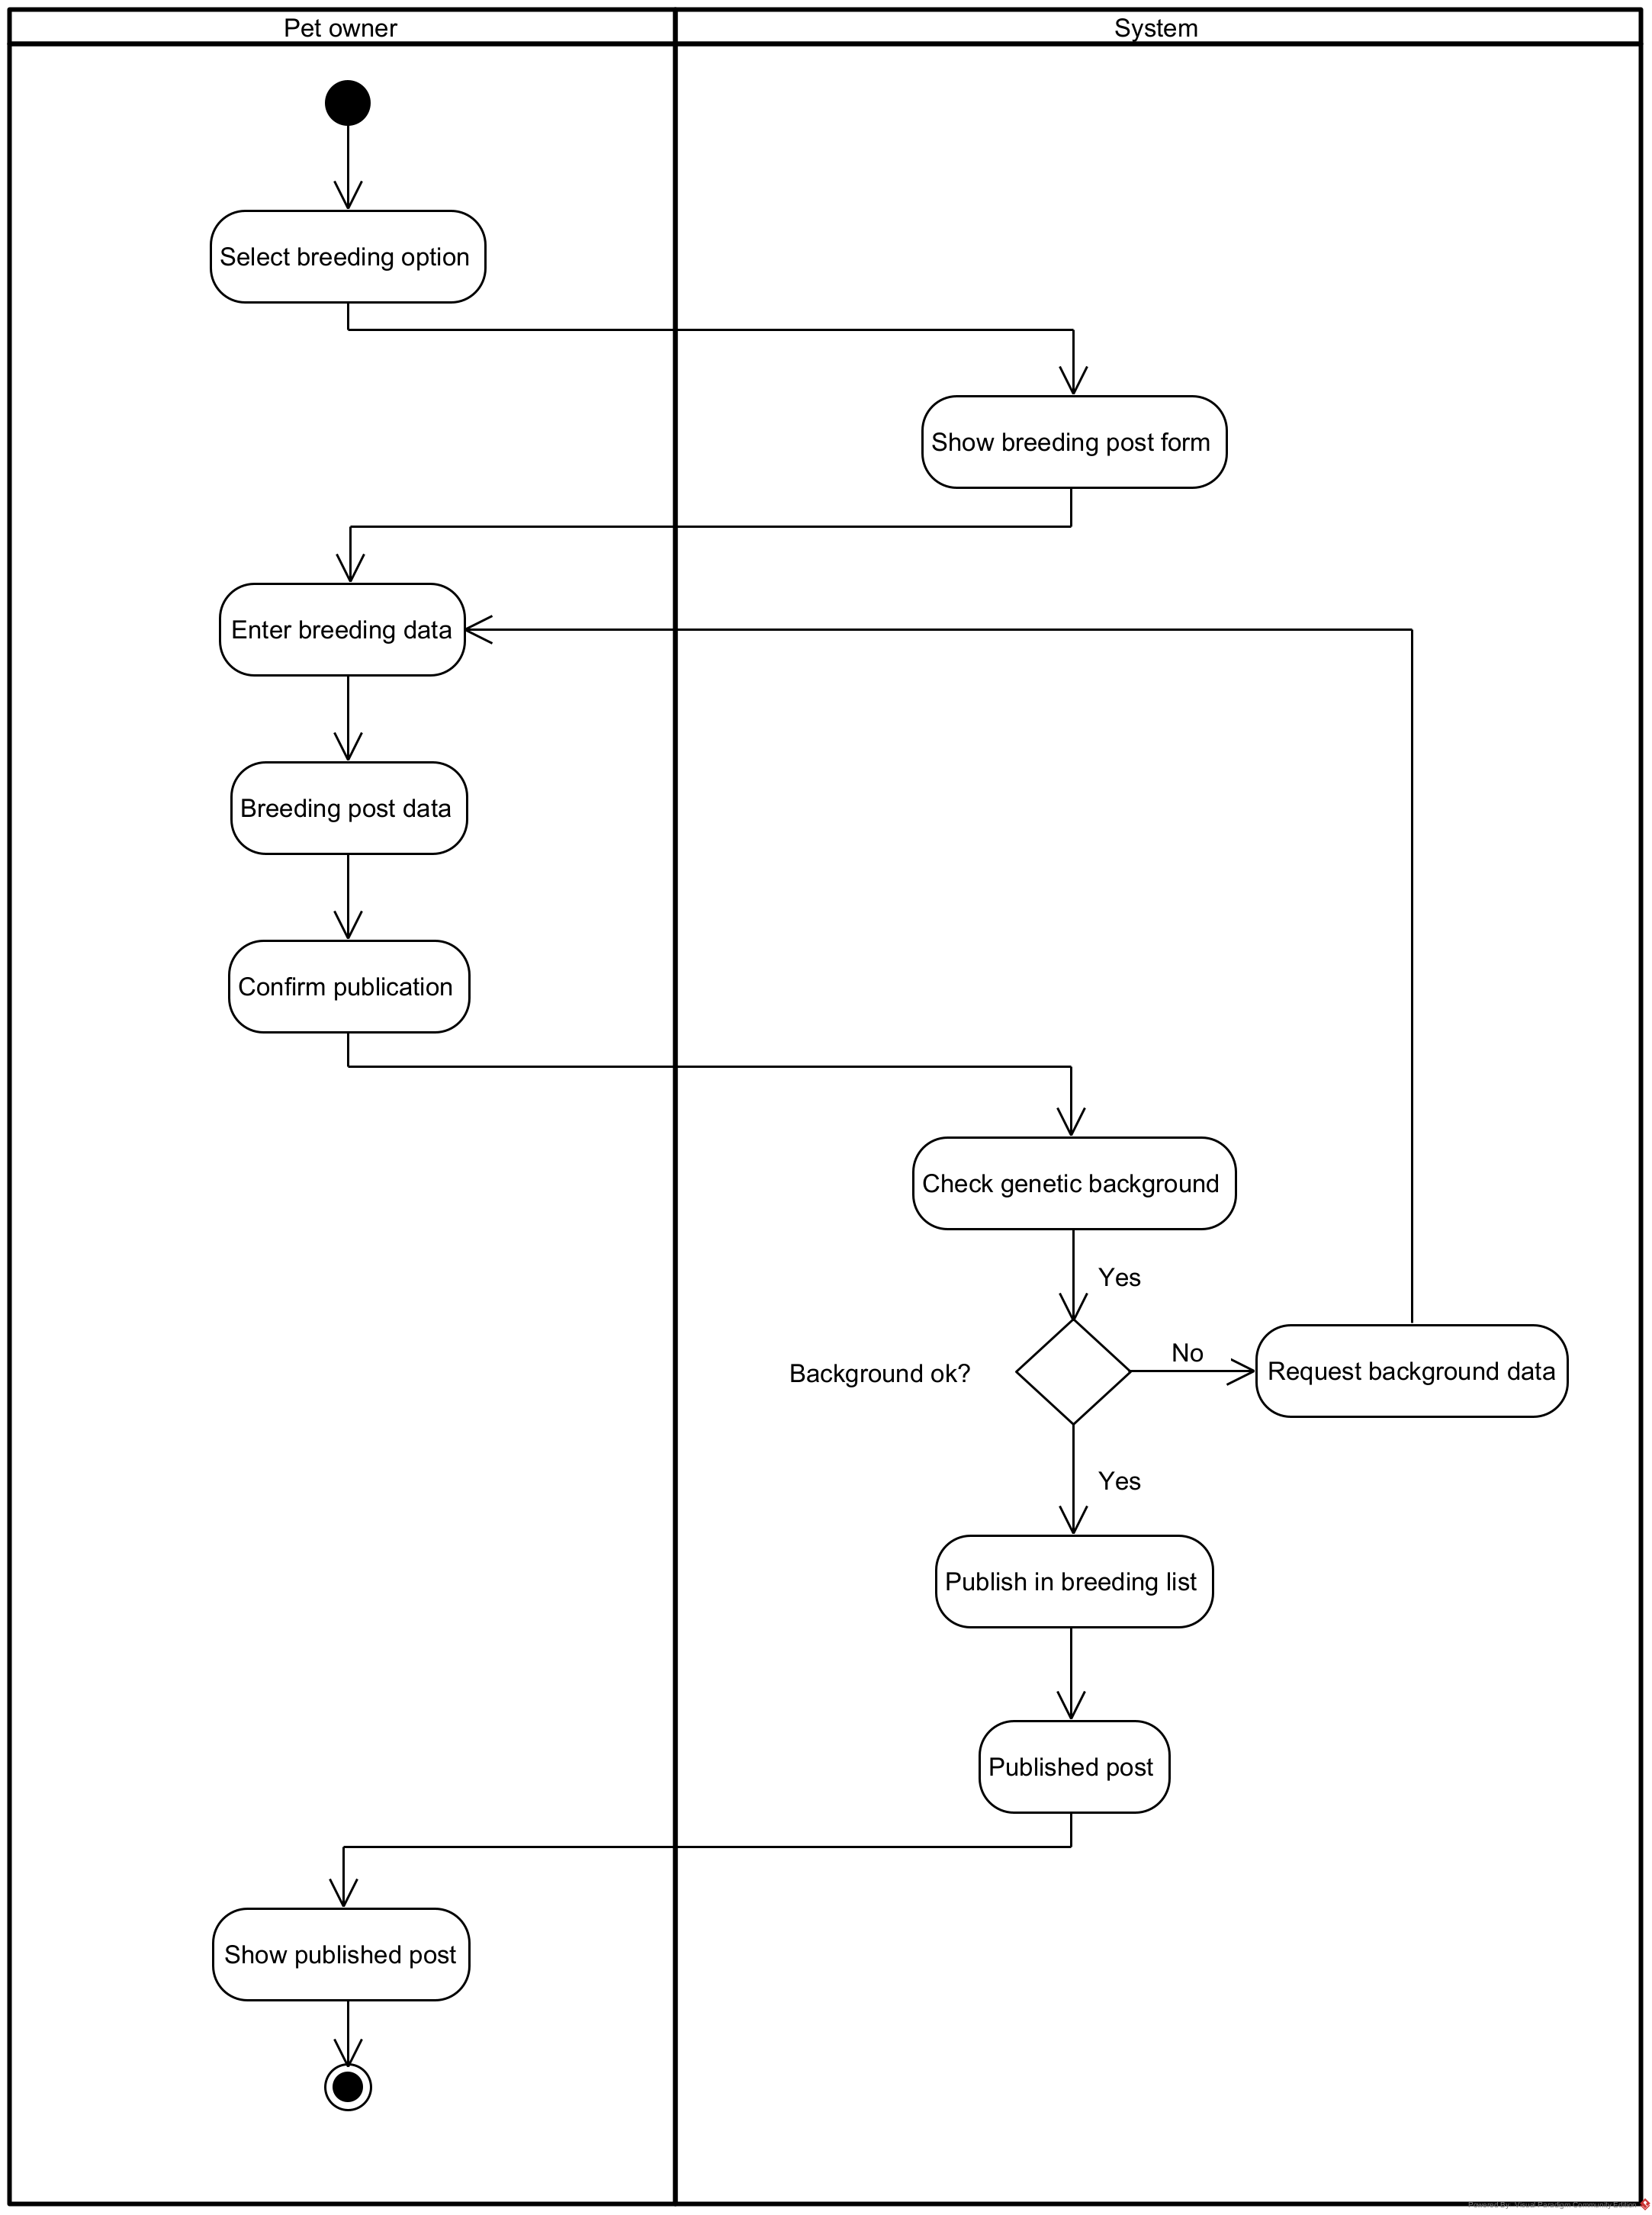
\includegraphics[width=0.75\textwidth]{figuras/DiagramaActividades_CU-05_MundiPets.png}
		\caption{Diagrama de actividad del caso de uso CU-05 --- Publicar mascota para cruza.}
		\label{fig:act-cu05}
	\end{figure}

	\subsubsection{Configurar privacidad médica (contenido real del archivo CU-06)}

	El diagrama de actividad de \texttt{DiagramaActividades\_CU-06}
	--- correspondiente a CU-12 en la Sección~\ref{sec:cu-detallado} ---
	expone la lógica de decisión de la configuración de privacidad (RF-11).
	Tras seleccionar los datos a compartir y guardar la configuración, la
	bifurcación central (\emph{Field blocked?}) verifica si algún campo
	restringido es obligatorio para la validación veterinaria; en caso
	afirmativo, el sistema muestra una advertencia de visibilidad y no aplica
	esa restricción puntual, mientras que en caso negativo almacena la
	configuración completa y actualiza los permisos.

	\begin{figure}[H]
		\centering
		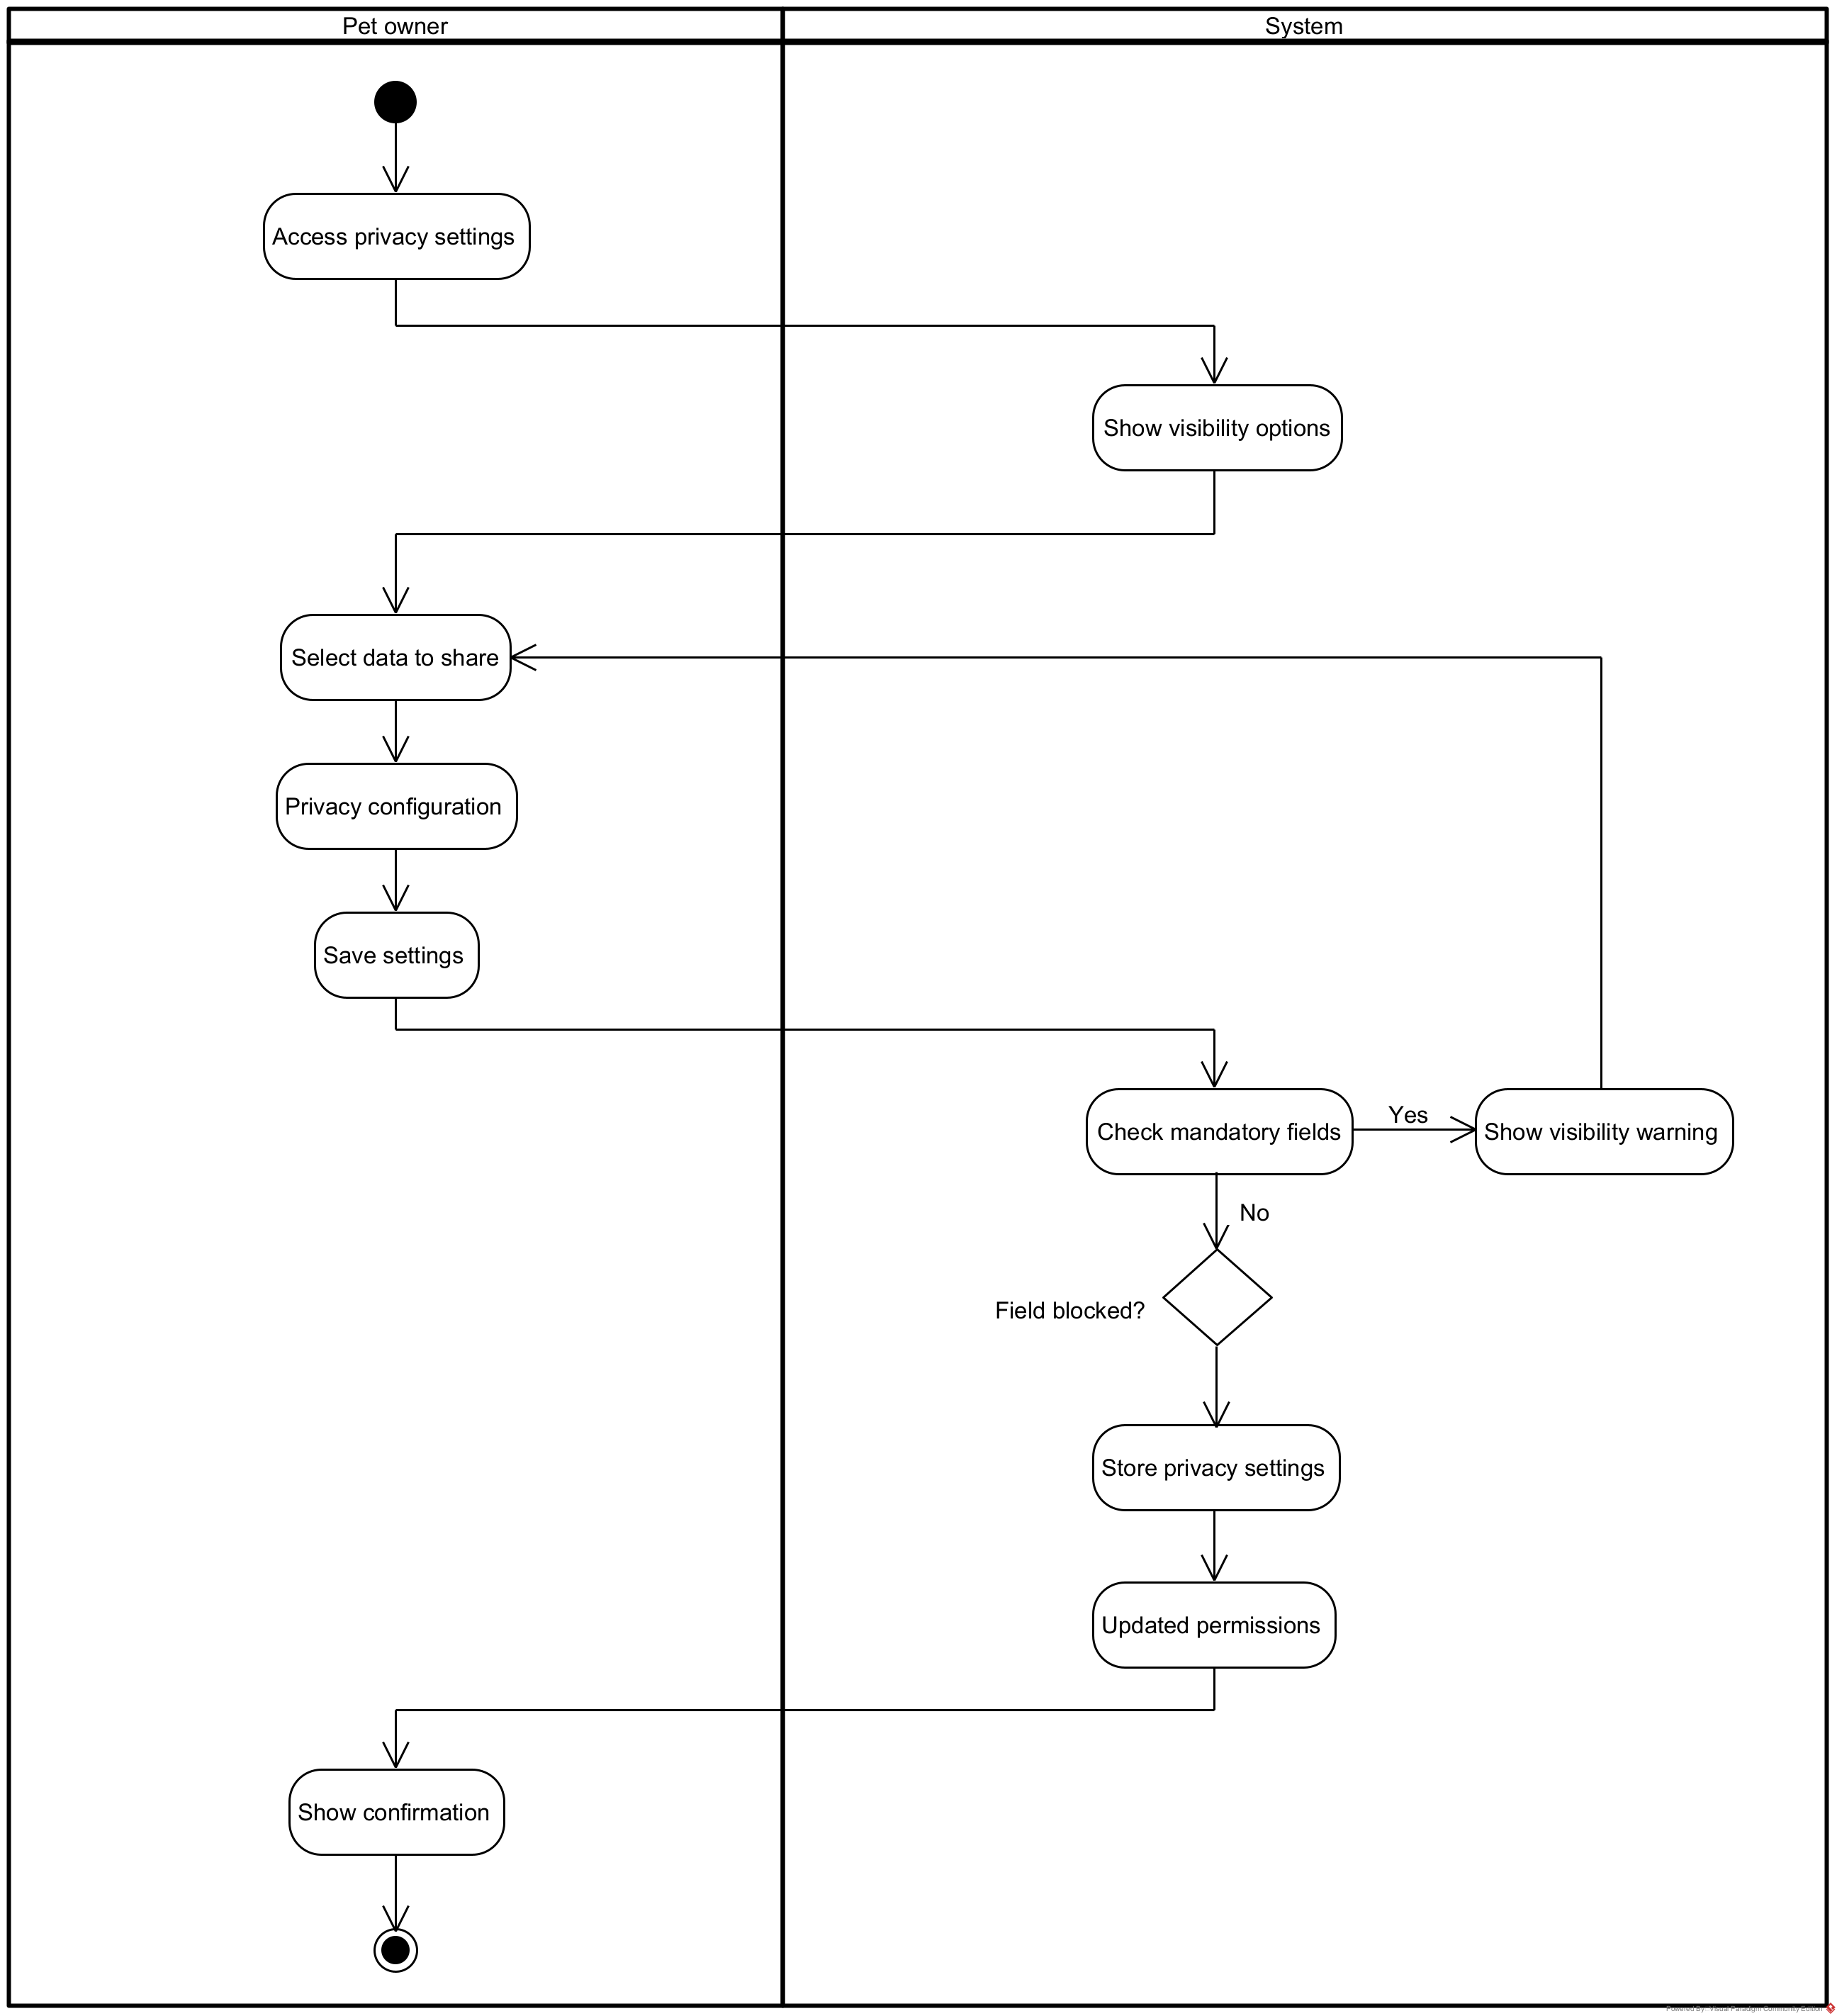
\includegraphics[width=0.90\textwidth]{figuras/DiagramaActividades_CU-06_MundiPets.png}
		\caption{Diagrama de actividad --- Configurar privacidad médica (archivo etiquetado CU-06; corresponde a CU-12).}
		\label{fig:act-cu06}
	\end{figure}

	\subsubsection{Gestionar solicitud de adopción (contenido real del archivo CU-07)}

	Este diagrama modela el flujo de gestión de una solicitud de adopción ya
	enviada (RF-05, RF-18): tras consultar el perfil (CU-10) y enviar la
	solicitud, el sistema la registra como pendiente y notifica al propietario
	o refugio; este revisa la solicitud y decide aceptarla o rechazarla
	(\emph{Accept?}), y el sistema actualiza el estado correspondiente y
	notifica al adoptante antes de mostrarle el estado final de su solicitud.

	\begin{figure}[H]
		\centering
		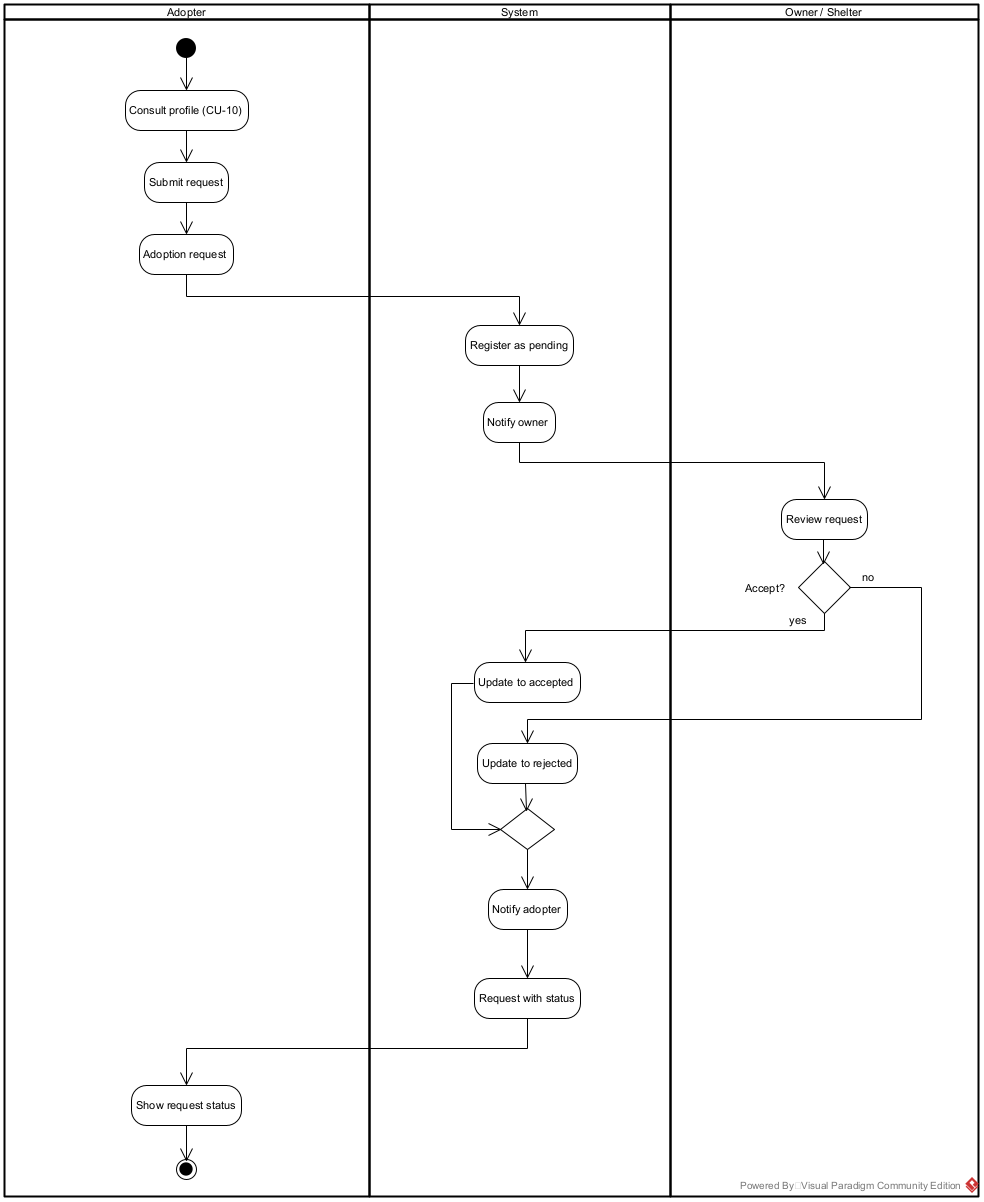
\includegraphics[width=0.82\textwidth]{figuras/DiagramaActividades_CU-07_MundiPets.png}
		\caption{Diagrama de actividad --- Gestionar solicitud de adopción (archivo etiquetado CU-07).}
		\label{fig:act-cu07}
	\end{figure}

	\subsubsection{Gestionar comunicación entre usuarios (CU-08)}

	El diagrama de actividad de CU-08 detalla el flujo de envío de un mensaje
	entre usuarios (RF-07): el sistema busca la conversación existente entre
	ambos usuarios o crea una nueva si es la primera interacción, almacena el
	mensaje y notifica al destinatario. El diagrama no representa una
	bifurcación de moderación automática de contenido; el mecanismo de reporte
	manual y la explicación por ejemplos de RNF-15 se documentan en la
	especificación textual de RF-07, no como una actividad de este flujo de
	envío.

	\begin{figure}[H]
		\centering
		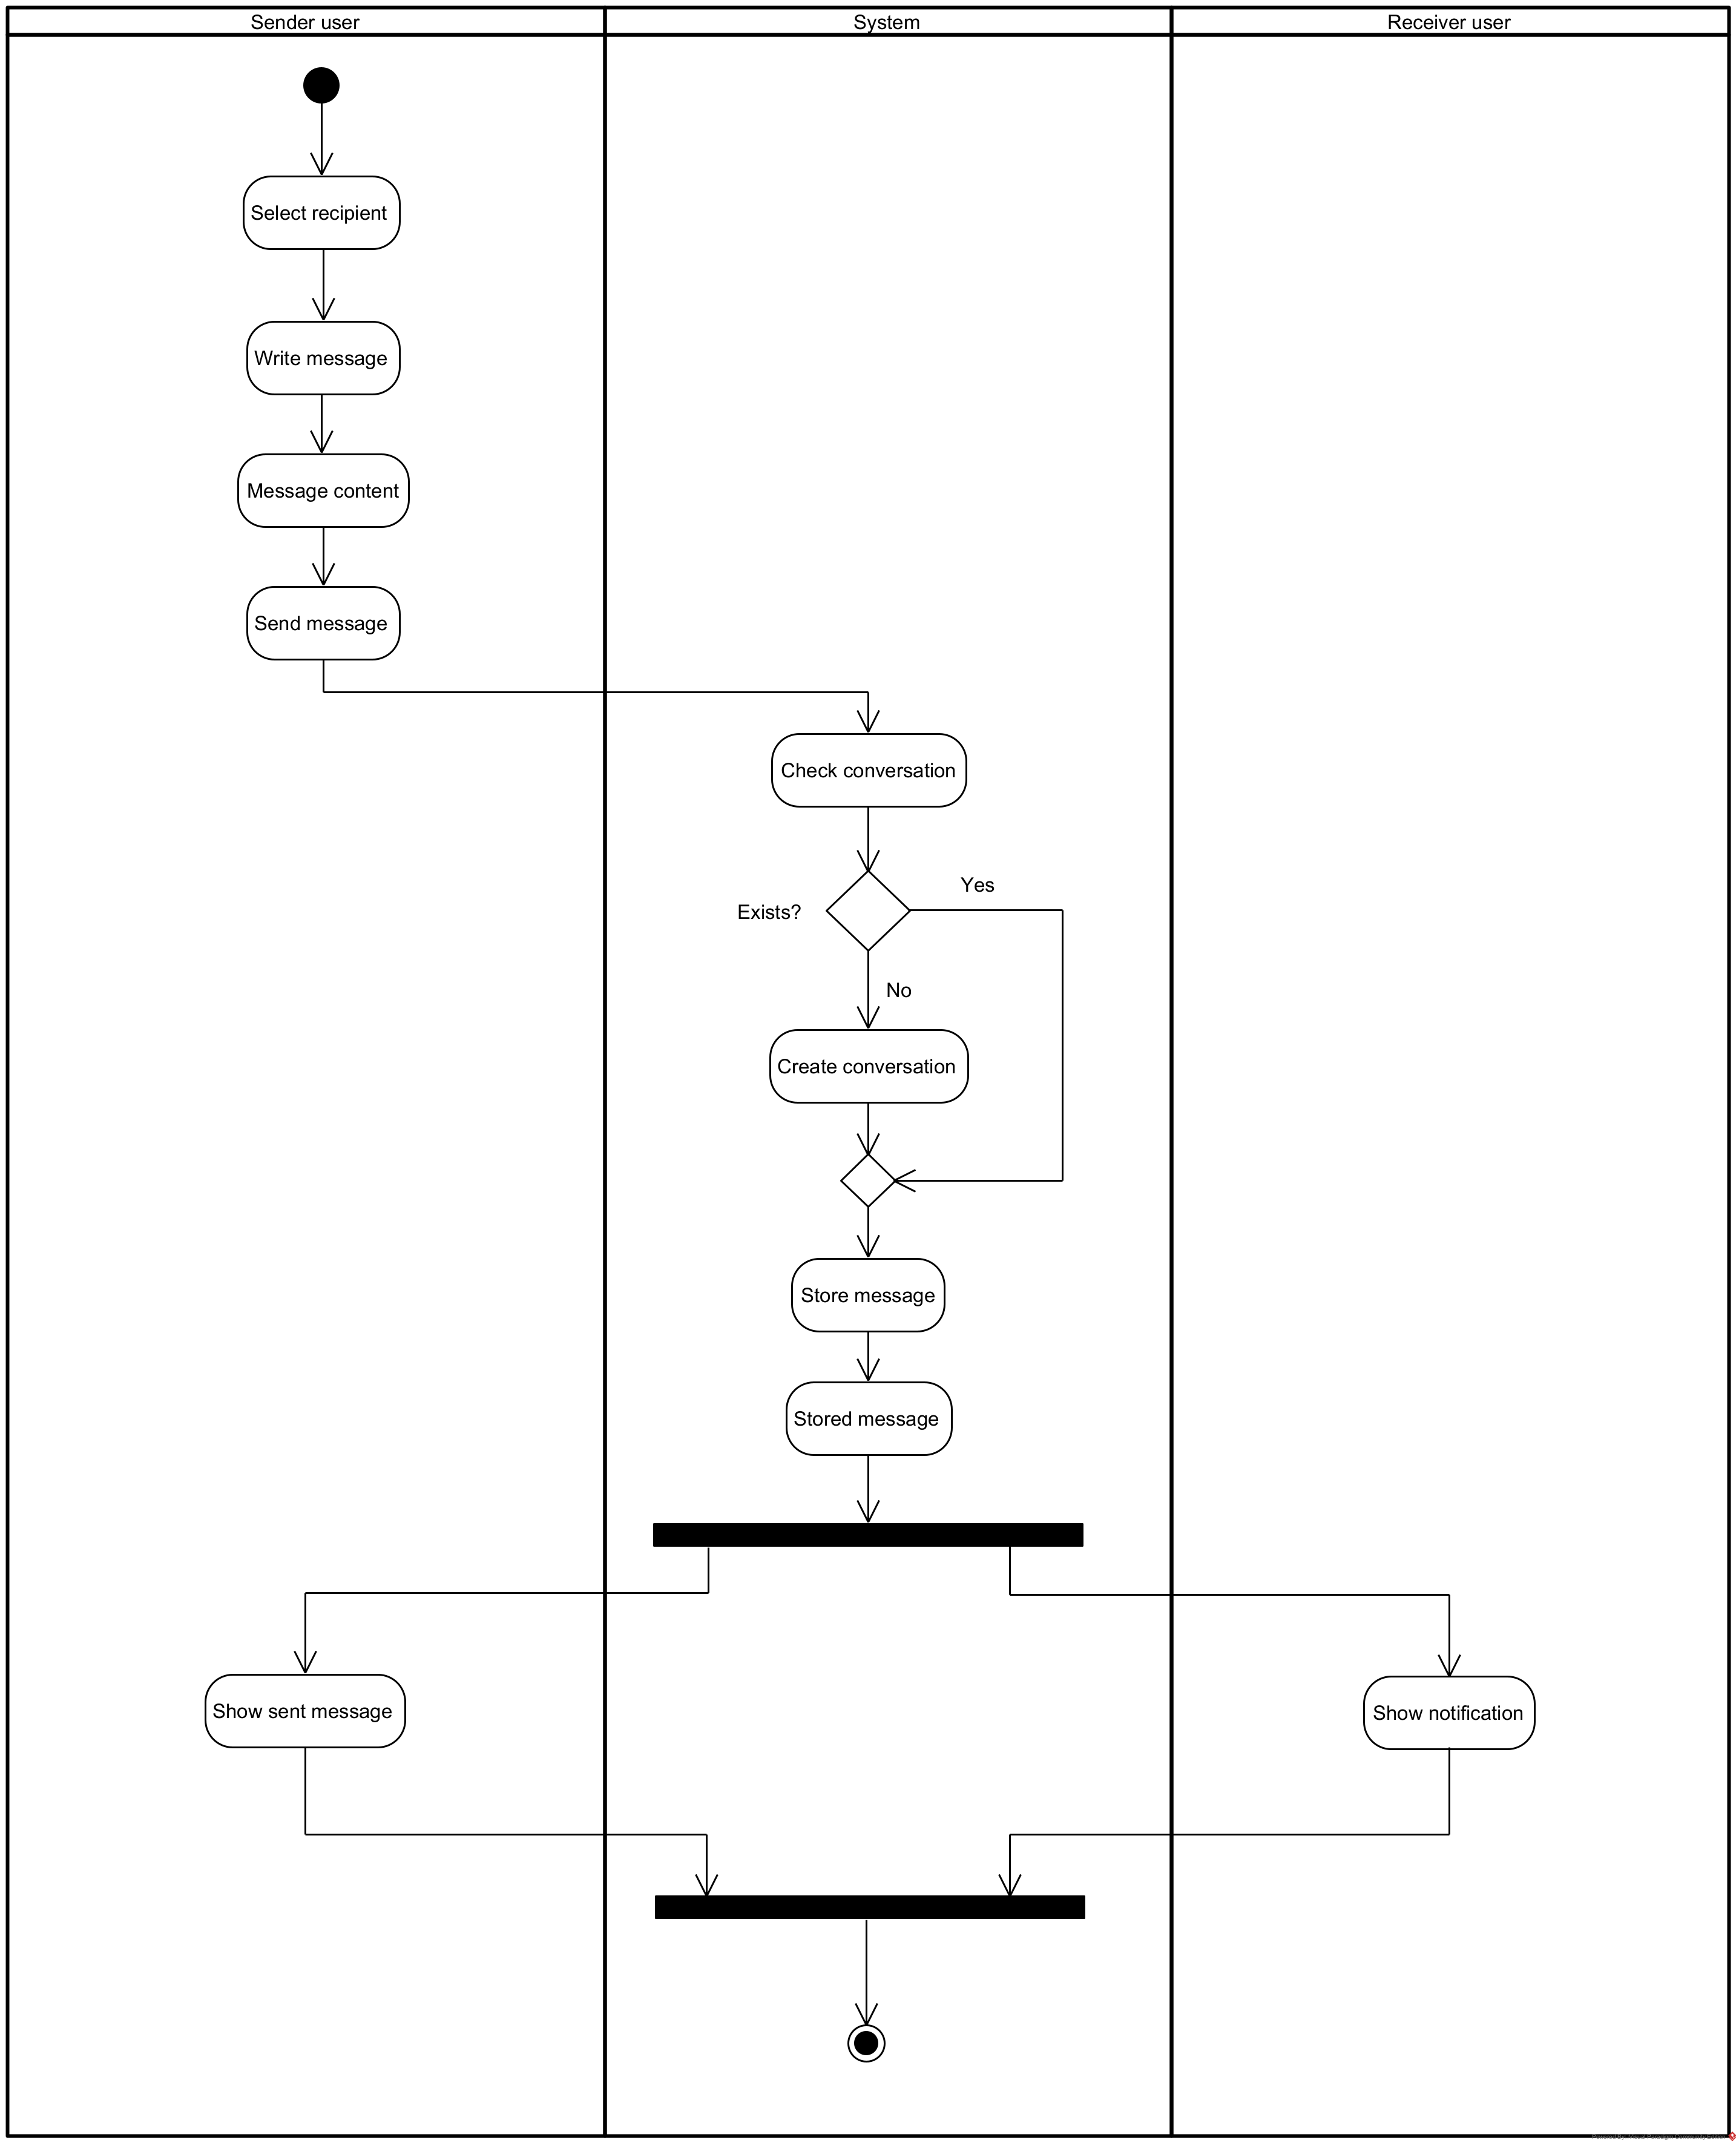
\includegraphics[width=0.81\textwidth]{figuras/DiagramaActividades_CU-08_MundiPets.png}
		\caption{Diagrama de actividad del caso de uso CU-08 --- Gestionar comunicación entre usuarios.}
		\label{fig:act-cu08}
	\end{figure}

	\subsubsection{Validar información médica (CU-09)}

	Este diagrama representa el flujo de revisión que ejecuta la veterinaria
	sobre el historial médico y los documentos cargados (RF-09). La
	bifurcación principal separa el camino de validación exitosa, que
	actualiza el estado del registro y lo asocia con la identificación de la
	veterinaria, del camino de rechazo, que exige registrar el motivo de la
	inconsistencia antes de notificar al propietario, en coherencia con la
	máquina de estados de verificación de documentos presentada en la
	Sección~\ref{sec:estados}. La segunda opinión veterinaria de RF-26
	corresponde a una nueva ejecución de este mismo diagrama de actividad
	sobre un registro ya validado.

	\begin{figure}[H]
		\centering
		
\includegraphics[width=0.52\textwidth]{figuras/DiagramaActividades_CU-09_MundiPets.png}
		\caption{Diagrama de actividad del caso de uso CU-09 --- Validar información médica.}
		\label{fig:act-cu09}
	\end{figure}

	\subsubsection{Consultar perfil médico (CU-10)}

	El diagrama de actividad de CU-10 expone el flujo de consulta de perfil
	completo de una mascota (RF-03), incluyendo la verificación de permisos de
	visibilidad según la configuración de privacidad definida por el
	propietario (RF-11). El flujo culmina con la presentación diferenciada del
	perfil: información completa para usuarios con permisos, y una versión
	restringida para el resto.

	\begin{figure}[H]
		\centering
		
\includegraphics[width=0.80\textwidth]{figuras/DiagramaActividades_CU-10_MundiPets.png}
		\caption{Diagrama de actividad del caso de uso CU-10 --- Consultar perfil médico.}
		\label{fig:act-cu10}
	\end{figure}

	\subsubsection{Buscar mascota disponible (CU-11)}

	Este diagrama representa el flujo de búsqueda y filtrado de mascotas
	(RF-04). Tras la selección de criterios por parte del usuario, el sistema
	aplica los filtros sobre el conjunto de publicaciones activas y evalúa si
	existen resultados; en caso de no existir coincidencias, el flujo muestra
	un mensaje informativo en lugar de una lista vacía sin alternativas de
	acción.

	\begin{figure}[H]
		\centering
		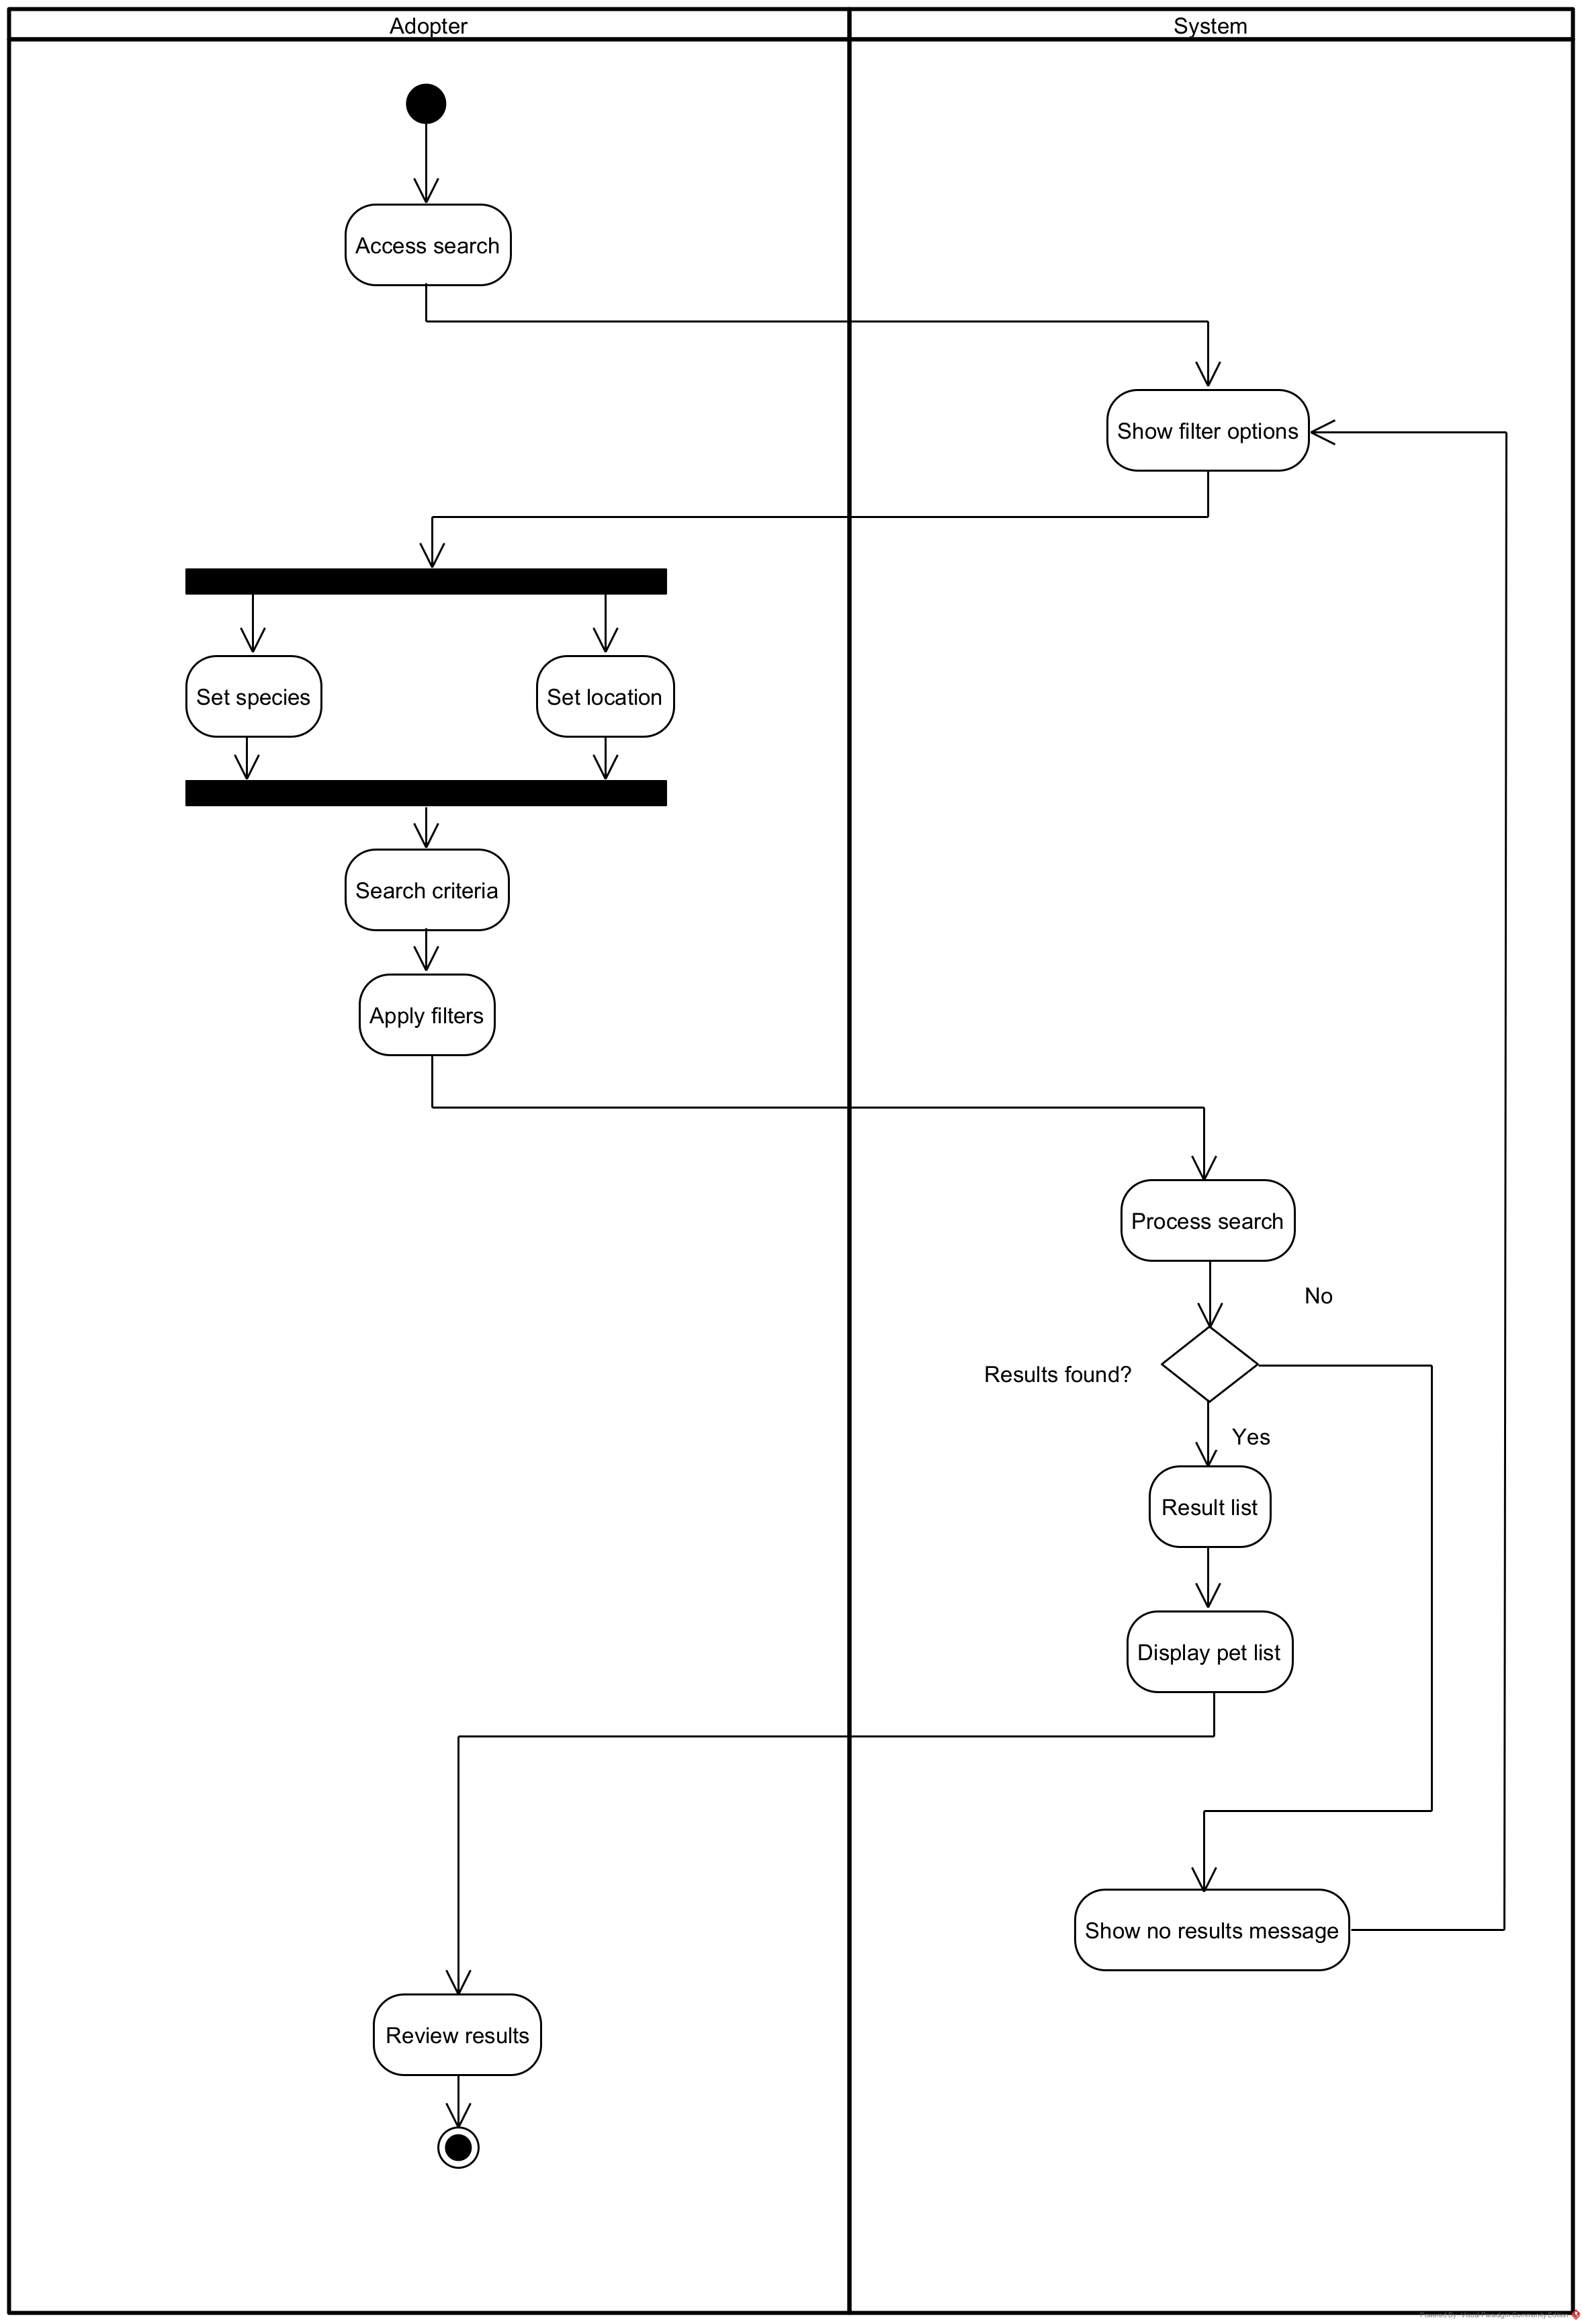
\includegraphics[width=0.73\textwidth]{figuras/DiagramaActividades_CU-11_MundiPets.png}
		\caption{Diagrama de actividad del caso de uso CU-11 --- Buscar mascota disponible.}
		\label{fig:act-cu11}
	\end{figure}

	\subsubsection{Consultar recomendaciones de cuidado (contenido real del archivo CU-12)}

	El diagrama de actividad de \texttt{DiagramaActividades\_CU-12} representa
	la consulta de recomendaciones de cuidado preventivo asociada a RF-10, el
	caso de uso de apoyo \emph{Check care recommendations} del diagrama
	general que no cuenta con número CU propio en la especificación textual.
	El sistema obtiene los datos de la mascota y, si la especie y la raza
	están especificadas, consulta las pautas correspondientes y las vacunas
	pendientes para presentar una recomendación específica; si falta alguno de
	esos datos, presenta en su lugar una recomendación básica genérica.

	\begin{figure}[H]
		\centering
		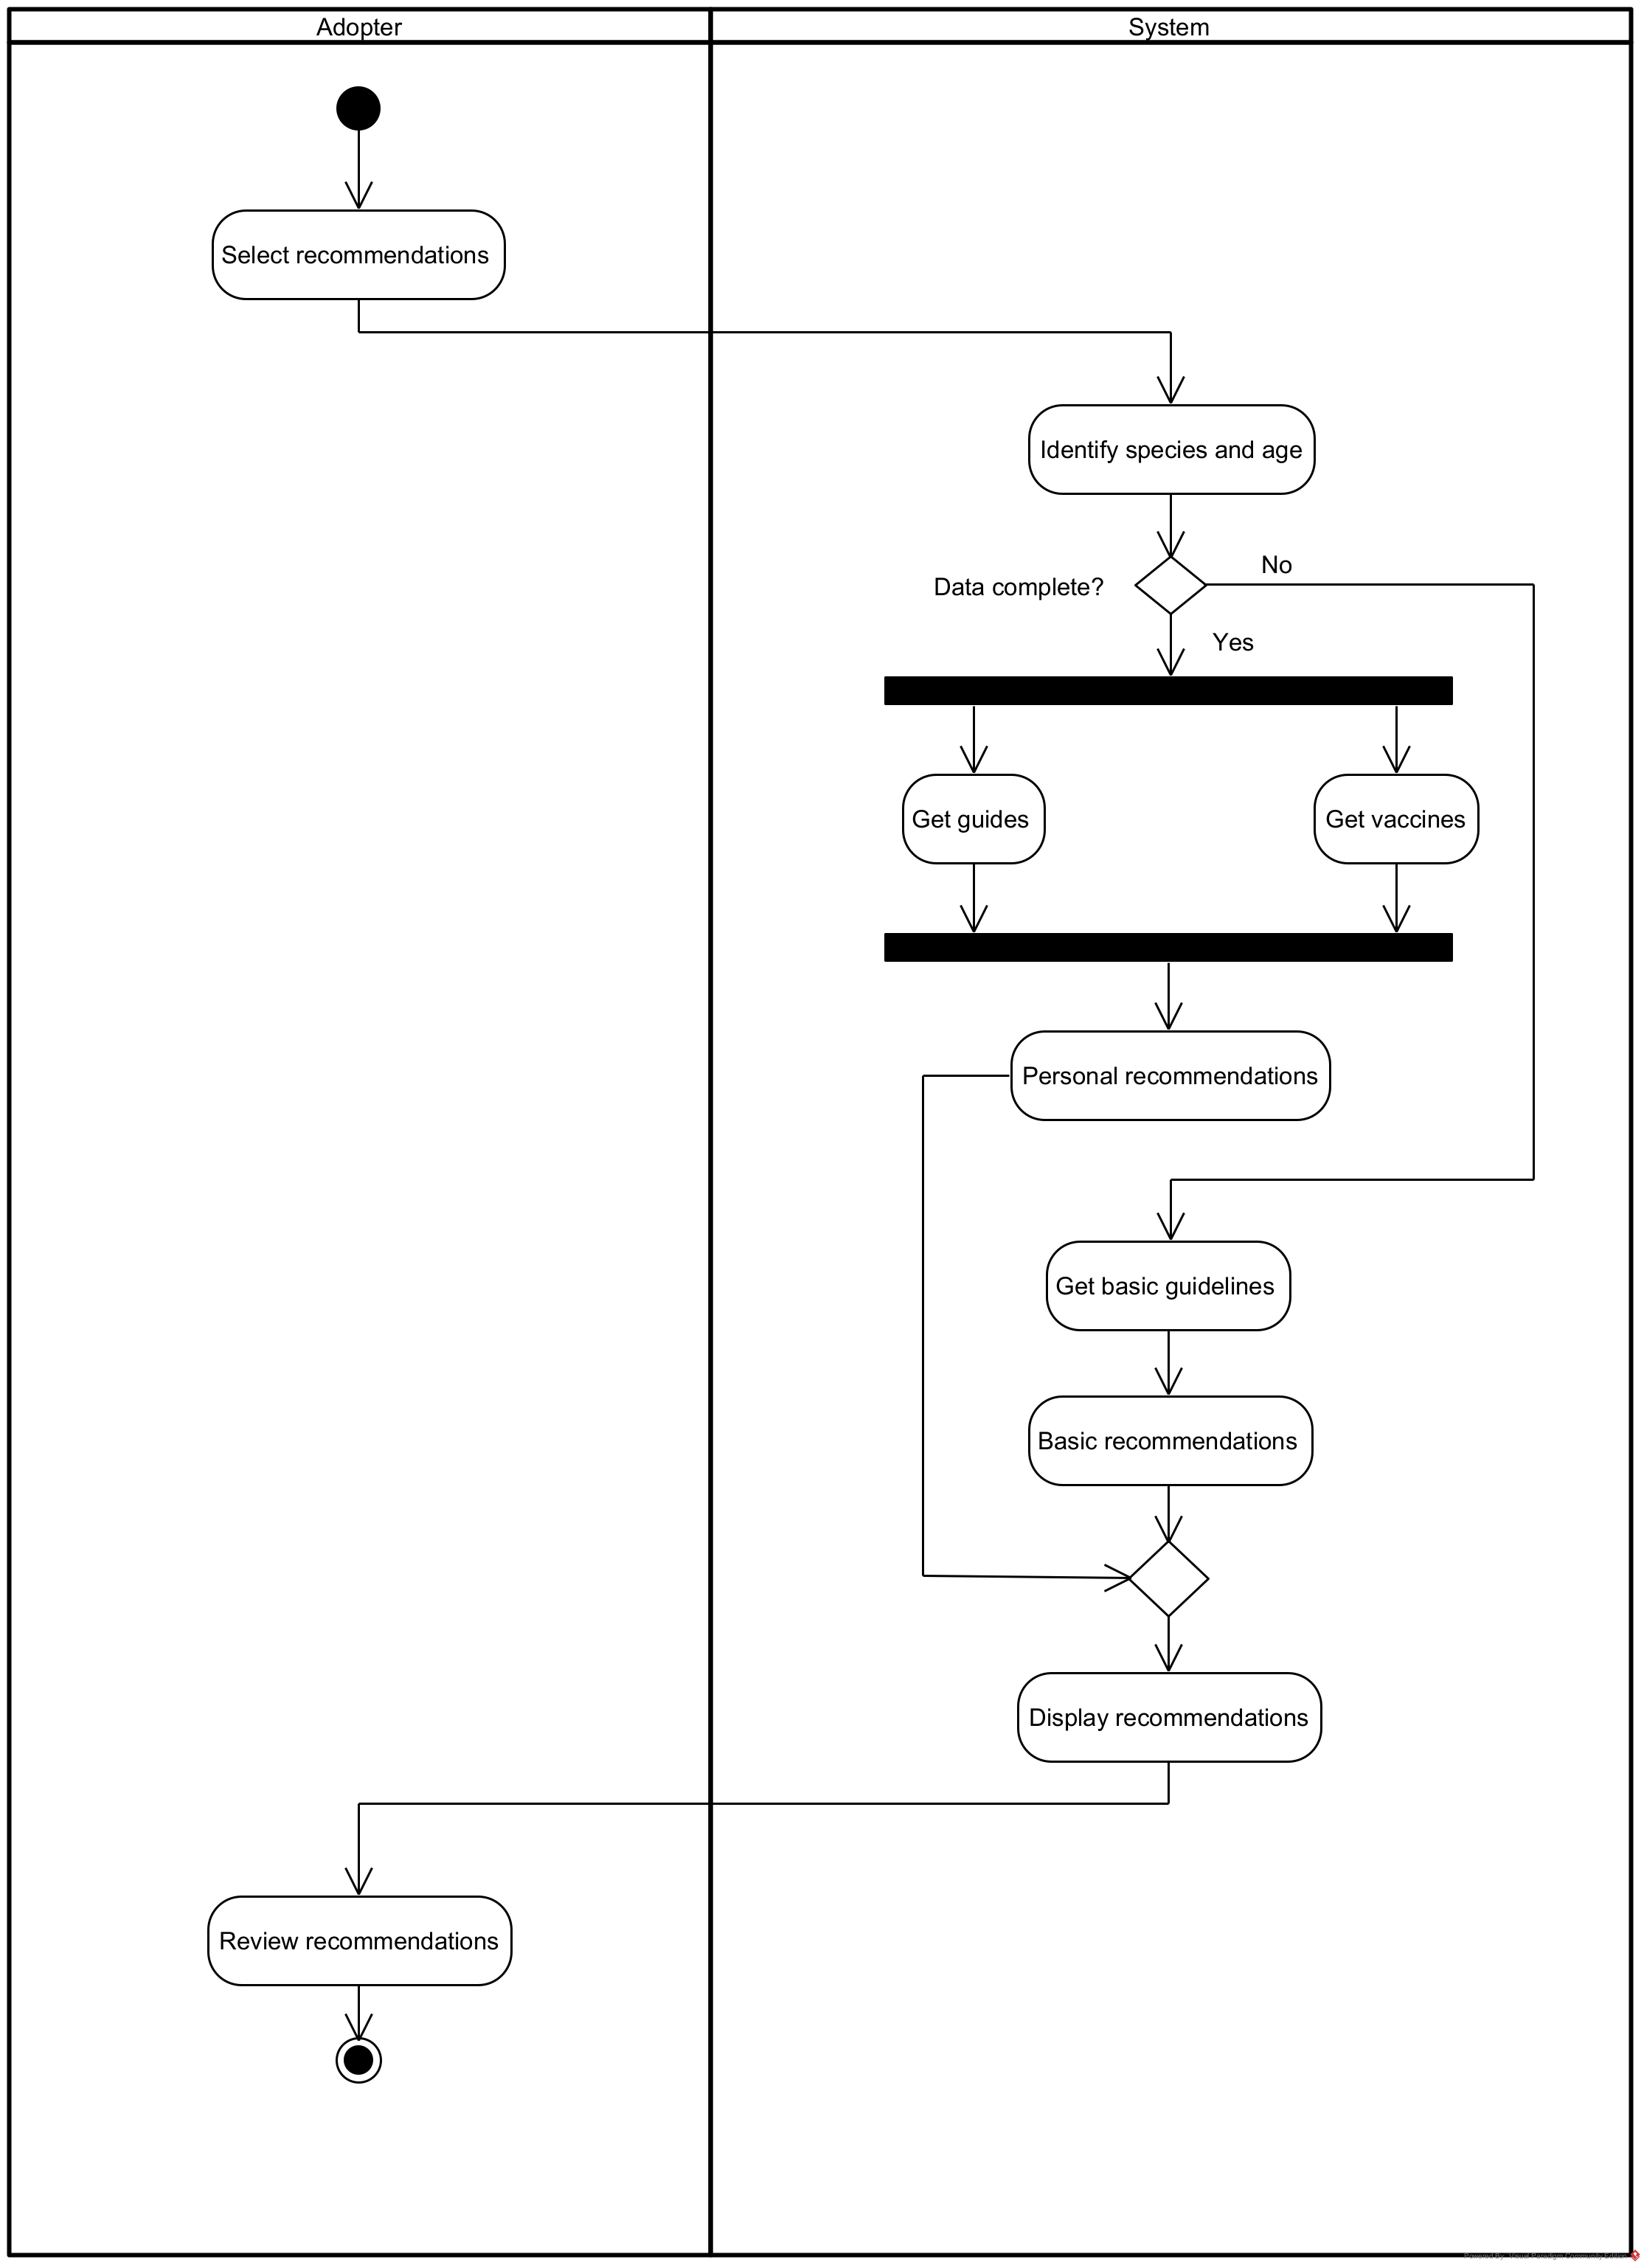
\includegraphics[width=0.73\textwidth]{figuras/DiagramaActividades_CU-12_MundiPets.png}
		\caption{Diagrama de actividad --- Consultar recomendaciones de cuidado (archivo etiquetado CU-12).}
		\label{fig:act-cu12}
	\end{figure}

	\subsubsection{Evaluar compatibilidad de cruza y verificación de parentesco (contenido real del archivo CU-13)}

	Este diagrama --- correspondiente a CU-06 y CU-13 en la
	Sección~\ref{sec:cu-detallado} --- expone la lógica de decisión que
	subyace a la recomendación de compatibilidad, integrando en un solo flujo
	la verificación de parentesco y la evaluación por inteligencia artificial.
	Tras la selección de las dos mascotas y la extracción de su historial
	clínico, el sistema invoca al servicio externo de evaluación; la
	bifurcación final determina si el puntaje obtenido es igual o superior a
	0.85 y no existe consanguinidad, en cuyo caso emite el informe de
	compatibilidad, o si detecta un campo faltante o una relación
	consanguínea, en cuyo caso dirige el flujo hacia la alerta de riesgo
	biológico y finaliza sin generar una recomendación, evitando así que el
	sistema sugiera una cruza que la propia especificación textual del caso de
	uso (flujo alterno 3.1 de la Tabla~\ref{tab:CU-13}) considera inviable.

	\begin{figure}[H]
		\centering
		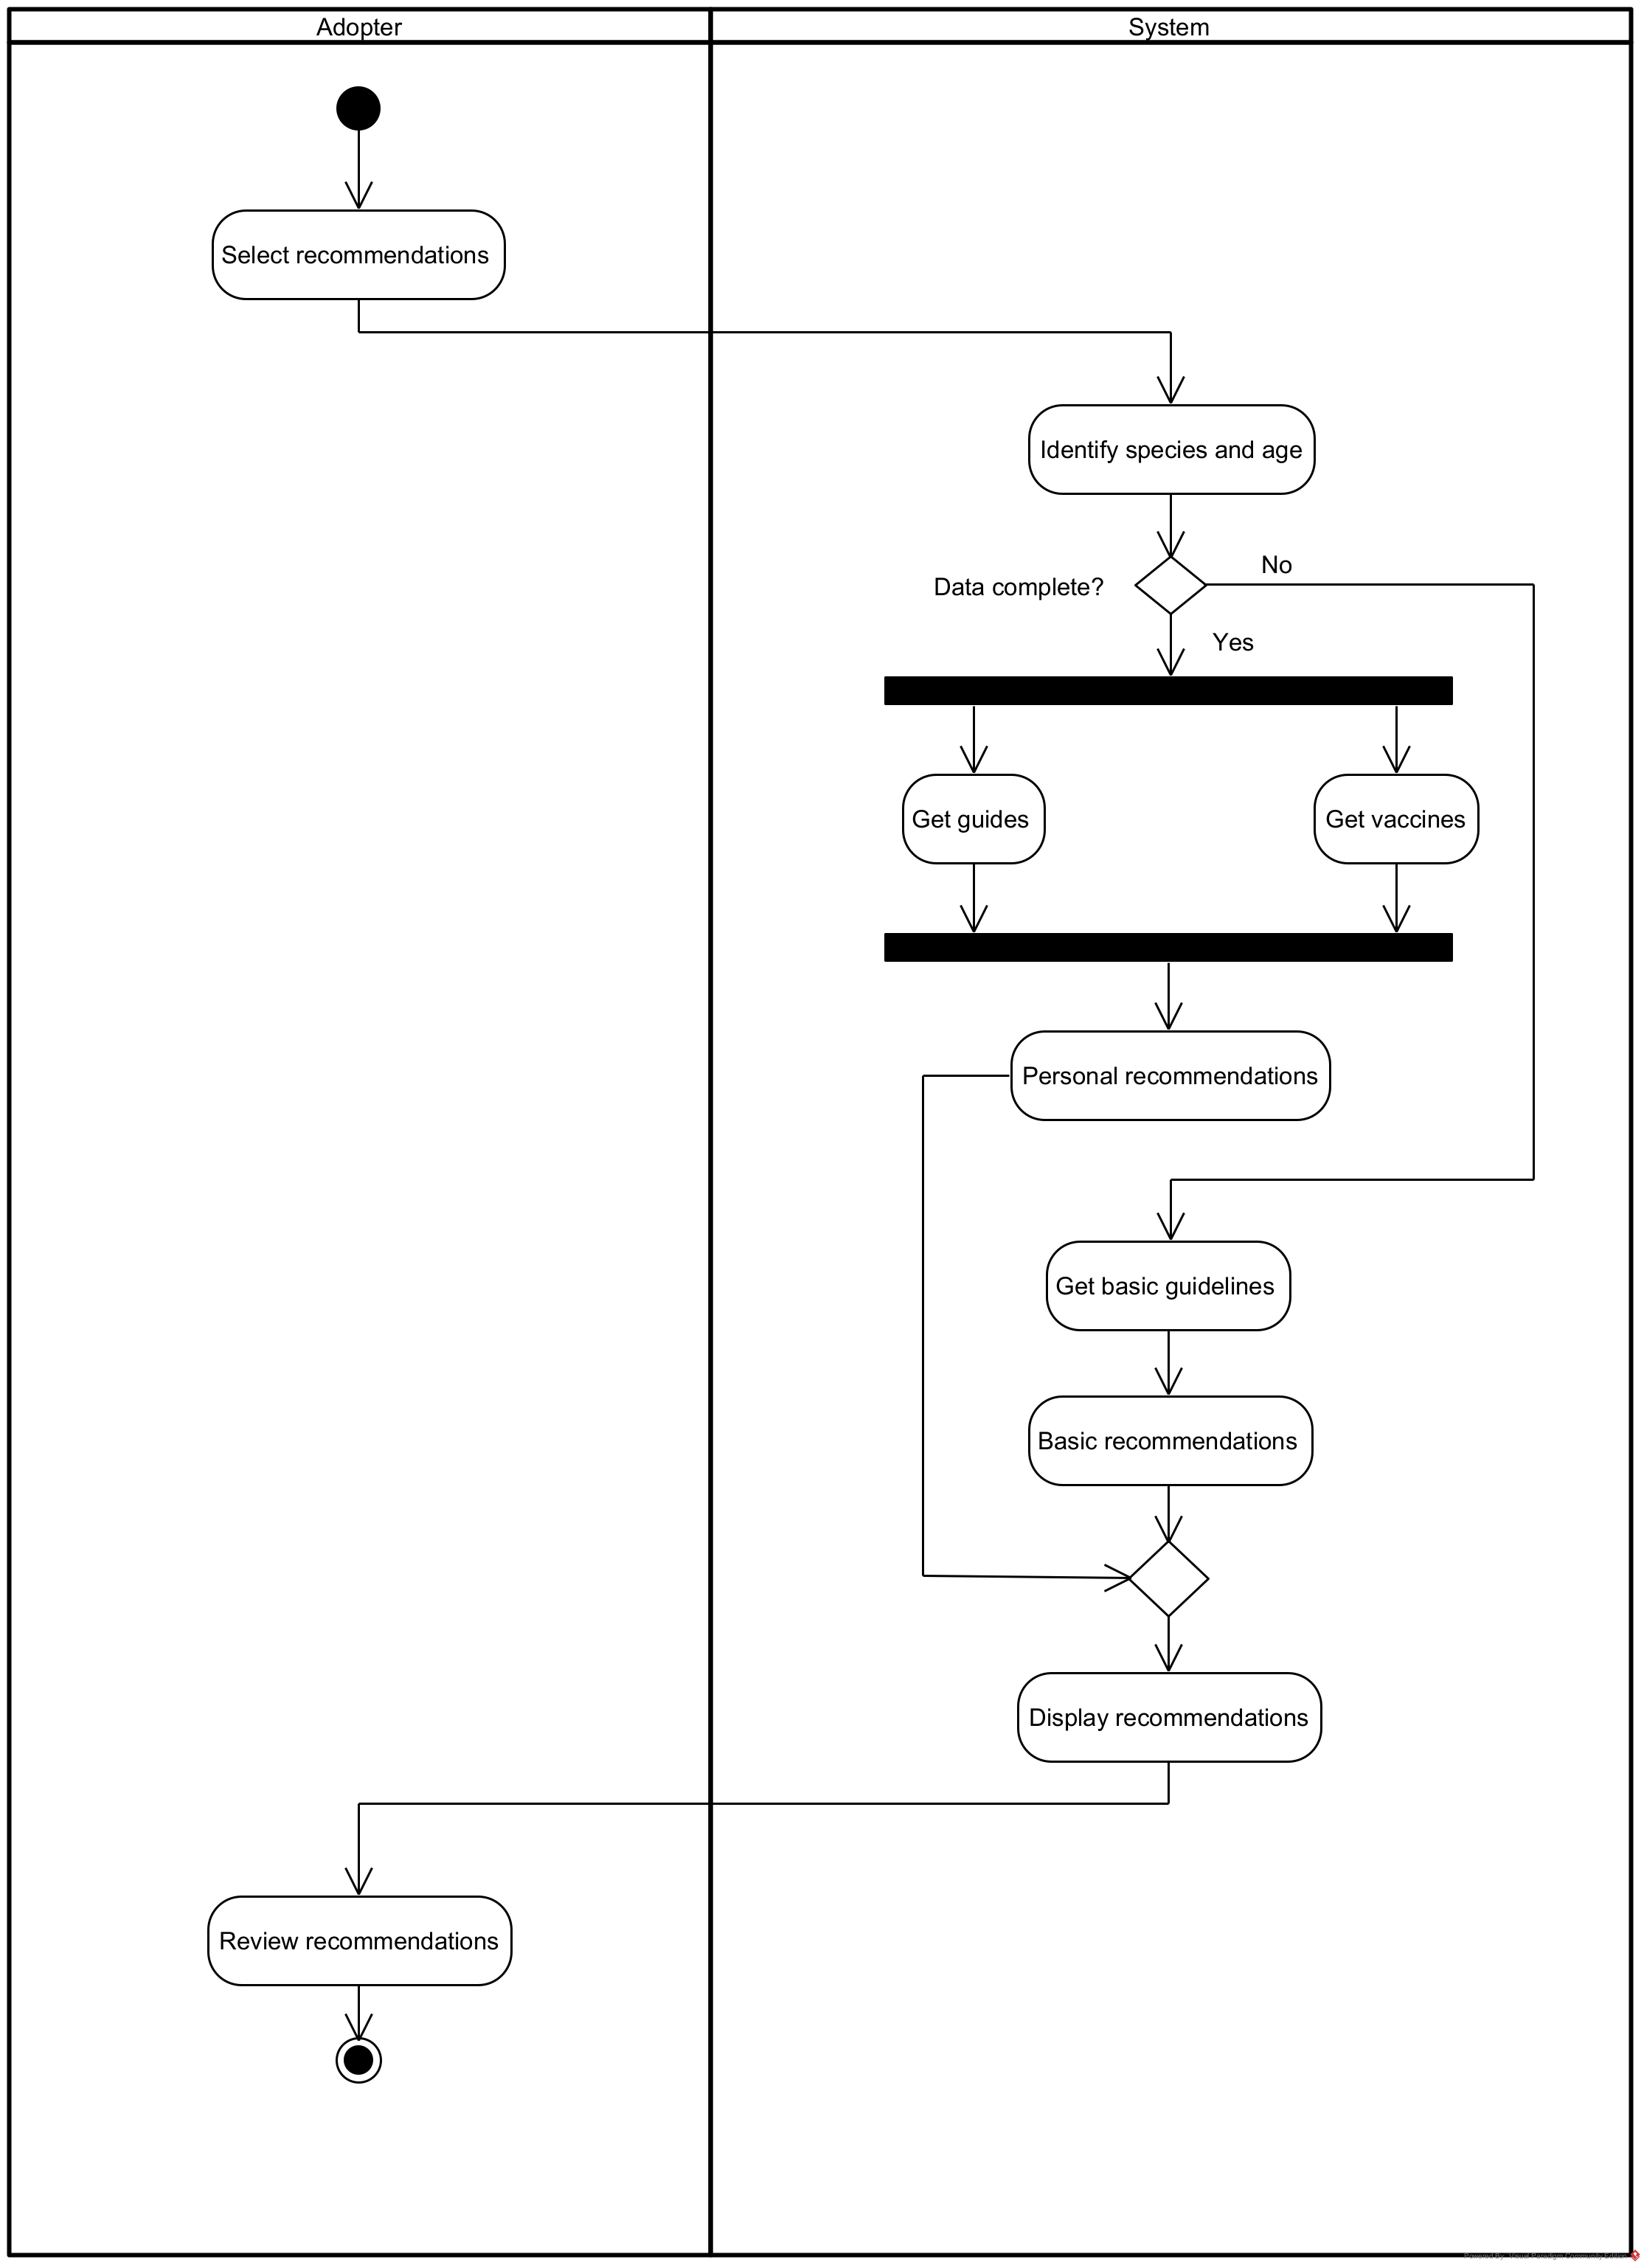
\includegraphics[width=1\textwidth]{figuras/DiagramaActividades_CU-13_MundiPets.png}
		\caption{Diagrama de actividad --- Evaluar compatibilidad de cruza y verificación de parentesco (archivo etiquetado CU-13; corresponde a CU-06 y CU-13).}
		\label{fig:act-cu13}
	\end{figure}

	\subsection{Diagrama de estados}
	\label{sec:estados}
	
	Se modelan tres máquinas de estado correspondientes a las entidades del
	sistema cuyo comportamiento depende fuertemente de transiciones bien
	definidas: el perfil de una mascota, una solicitud de adopción o cruza, y el
	proceso de verificación de documentos médicos. Estas tres entidades
	concentran la mayor parte de la lógica de negocio condicionada por el rol
	del usuario y por las validaciones cruzadas entre propietarios, adoptantes y
	veterinarias.
	
	\subsubsection{Estados del perfil de mascota}

	El ciclo de vida del perfil de una mascota inicia en el estado
	\emph{Drafted} al ejecutarse \texttt{registerPet()} (RF-01), y retorna a
	\emph{Drafted} si el propietario deja campos incompletos
	(\emph{notifyOwner()}). Al enviarse el formulario completo
	(\texttt{submitProfile()}) transita al estado compuesto \emph{Submitted},
	que verifica secuencialmente \emph{RequiredFieldsChecked},
	\emph{PhotosAndSpeciesChecked} --- donde se ejecuta la validación de
	imágenes exigida por RF-17 --- y \emph{SpeciesCompatibilityChecked}. Al
	completarse esta verificación (\texttt{publishProfile()}), el perfil
	alcanza el estado \emph{Published} (RF-13), desde el cual una solicitud
	recibida (\texttt{lockCandidate()}) lo lleva al estado compuesto
	\emph{matching process}: \emph{ApplicantReviewed},
	\emph{MeetingCoordinated} y \emph{OutcomeConfirmed}. Si el proceso se
	retira (\emph{withdraw}), el perfil regresa a \emph{Published}; si se
	confirma (\emph{matched?~=~yes}), el perfil alcanza el estado final
	\emph{adopted or matched}, en el que se habilita el seguimiento
	post-adopción definido por RF-22.

	\begin{figure}[H]
		\centering
		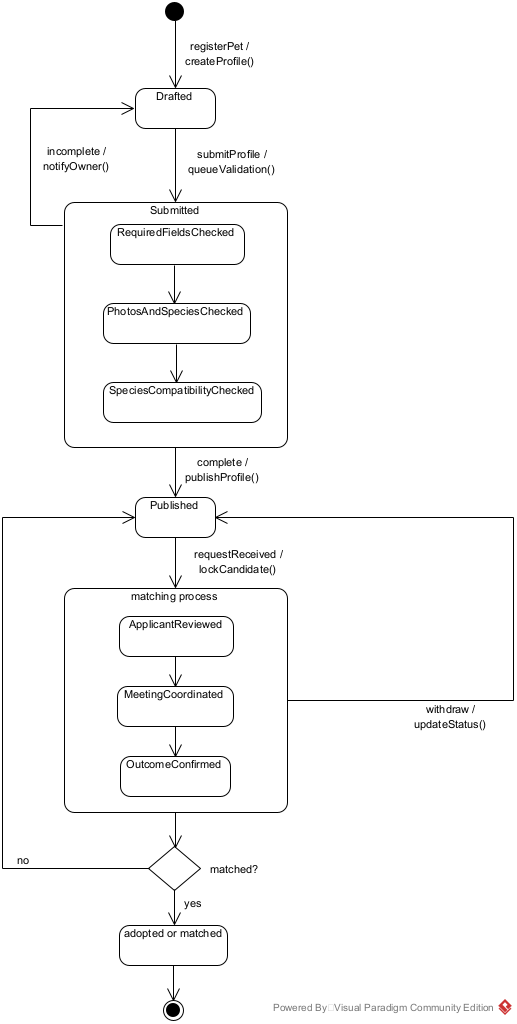
\includegraphics[width=0.50\textwidth]{figuras/DiagramaMaquinasEstado_PerfilMascota_MundiPets.png}
		\caption{Diagrama de estados del perfil de mascota.}
		\label{fig:est-mascota}
	\end{figure}

	\subsubsection{Estados de una solicitud de adopción o cruza}

	Esta máquina de estados formaliza el flujo por etapas exigido por RF-18
	para las solicitudes de adopción, y el flujo de aceptación o rechazo
	definido por RF-08 para las solicitudes de cruza. Una solicitud se crea
	en el estado \emph{Created} (\texttt{registerRequest()}) y transita a
	\emph{Submitted} al notificarse al propietario. Desde ahí, al iniciarse
	la revisión (\texttt{loadRequest()}), alcanza el estado compuesto
	\emph{Under review}, que verifica secuencialmente
	\emph{IdentityValidated} (RF-12), \emph{InformationReviewed} y
	\emph{RequestEvaluated}. Según el resultado de la evaluación, la
	solicitud transita a \emph{Approved} (\texttt{meetsRequirements}) o a
	\emph{Rejected} (\texttt{doesNotMeetRequirements}), ambos estados
	finales; en cualquier punto anterior a la resolución, la solicitud puede
	transitar a \emph{Cancelled} (\texttt{cancel}), desde donde se confirma
	su archivado (\texttt{confirmCancellation()}). Estas transiciones quedan
	registradas para alimentar la consulta de historial de procesos definida
	en RF-15. Cada transición de una solicitud de cruza hacia \emph{Approved}
	incrementa el contador de procesos completados de la mascota implicada,
	valor que RF-27 consulta antes de admitir una nueva solicitud sobre la
	misma mascota, sin introducir un estado adicional en esta máquina.

	\begin{figure}[H]
		\centering
		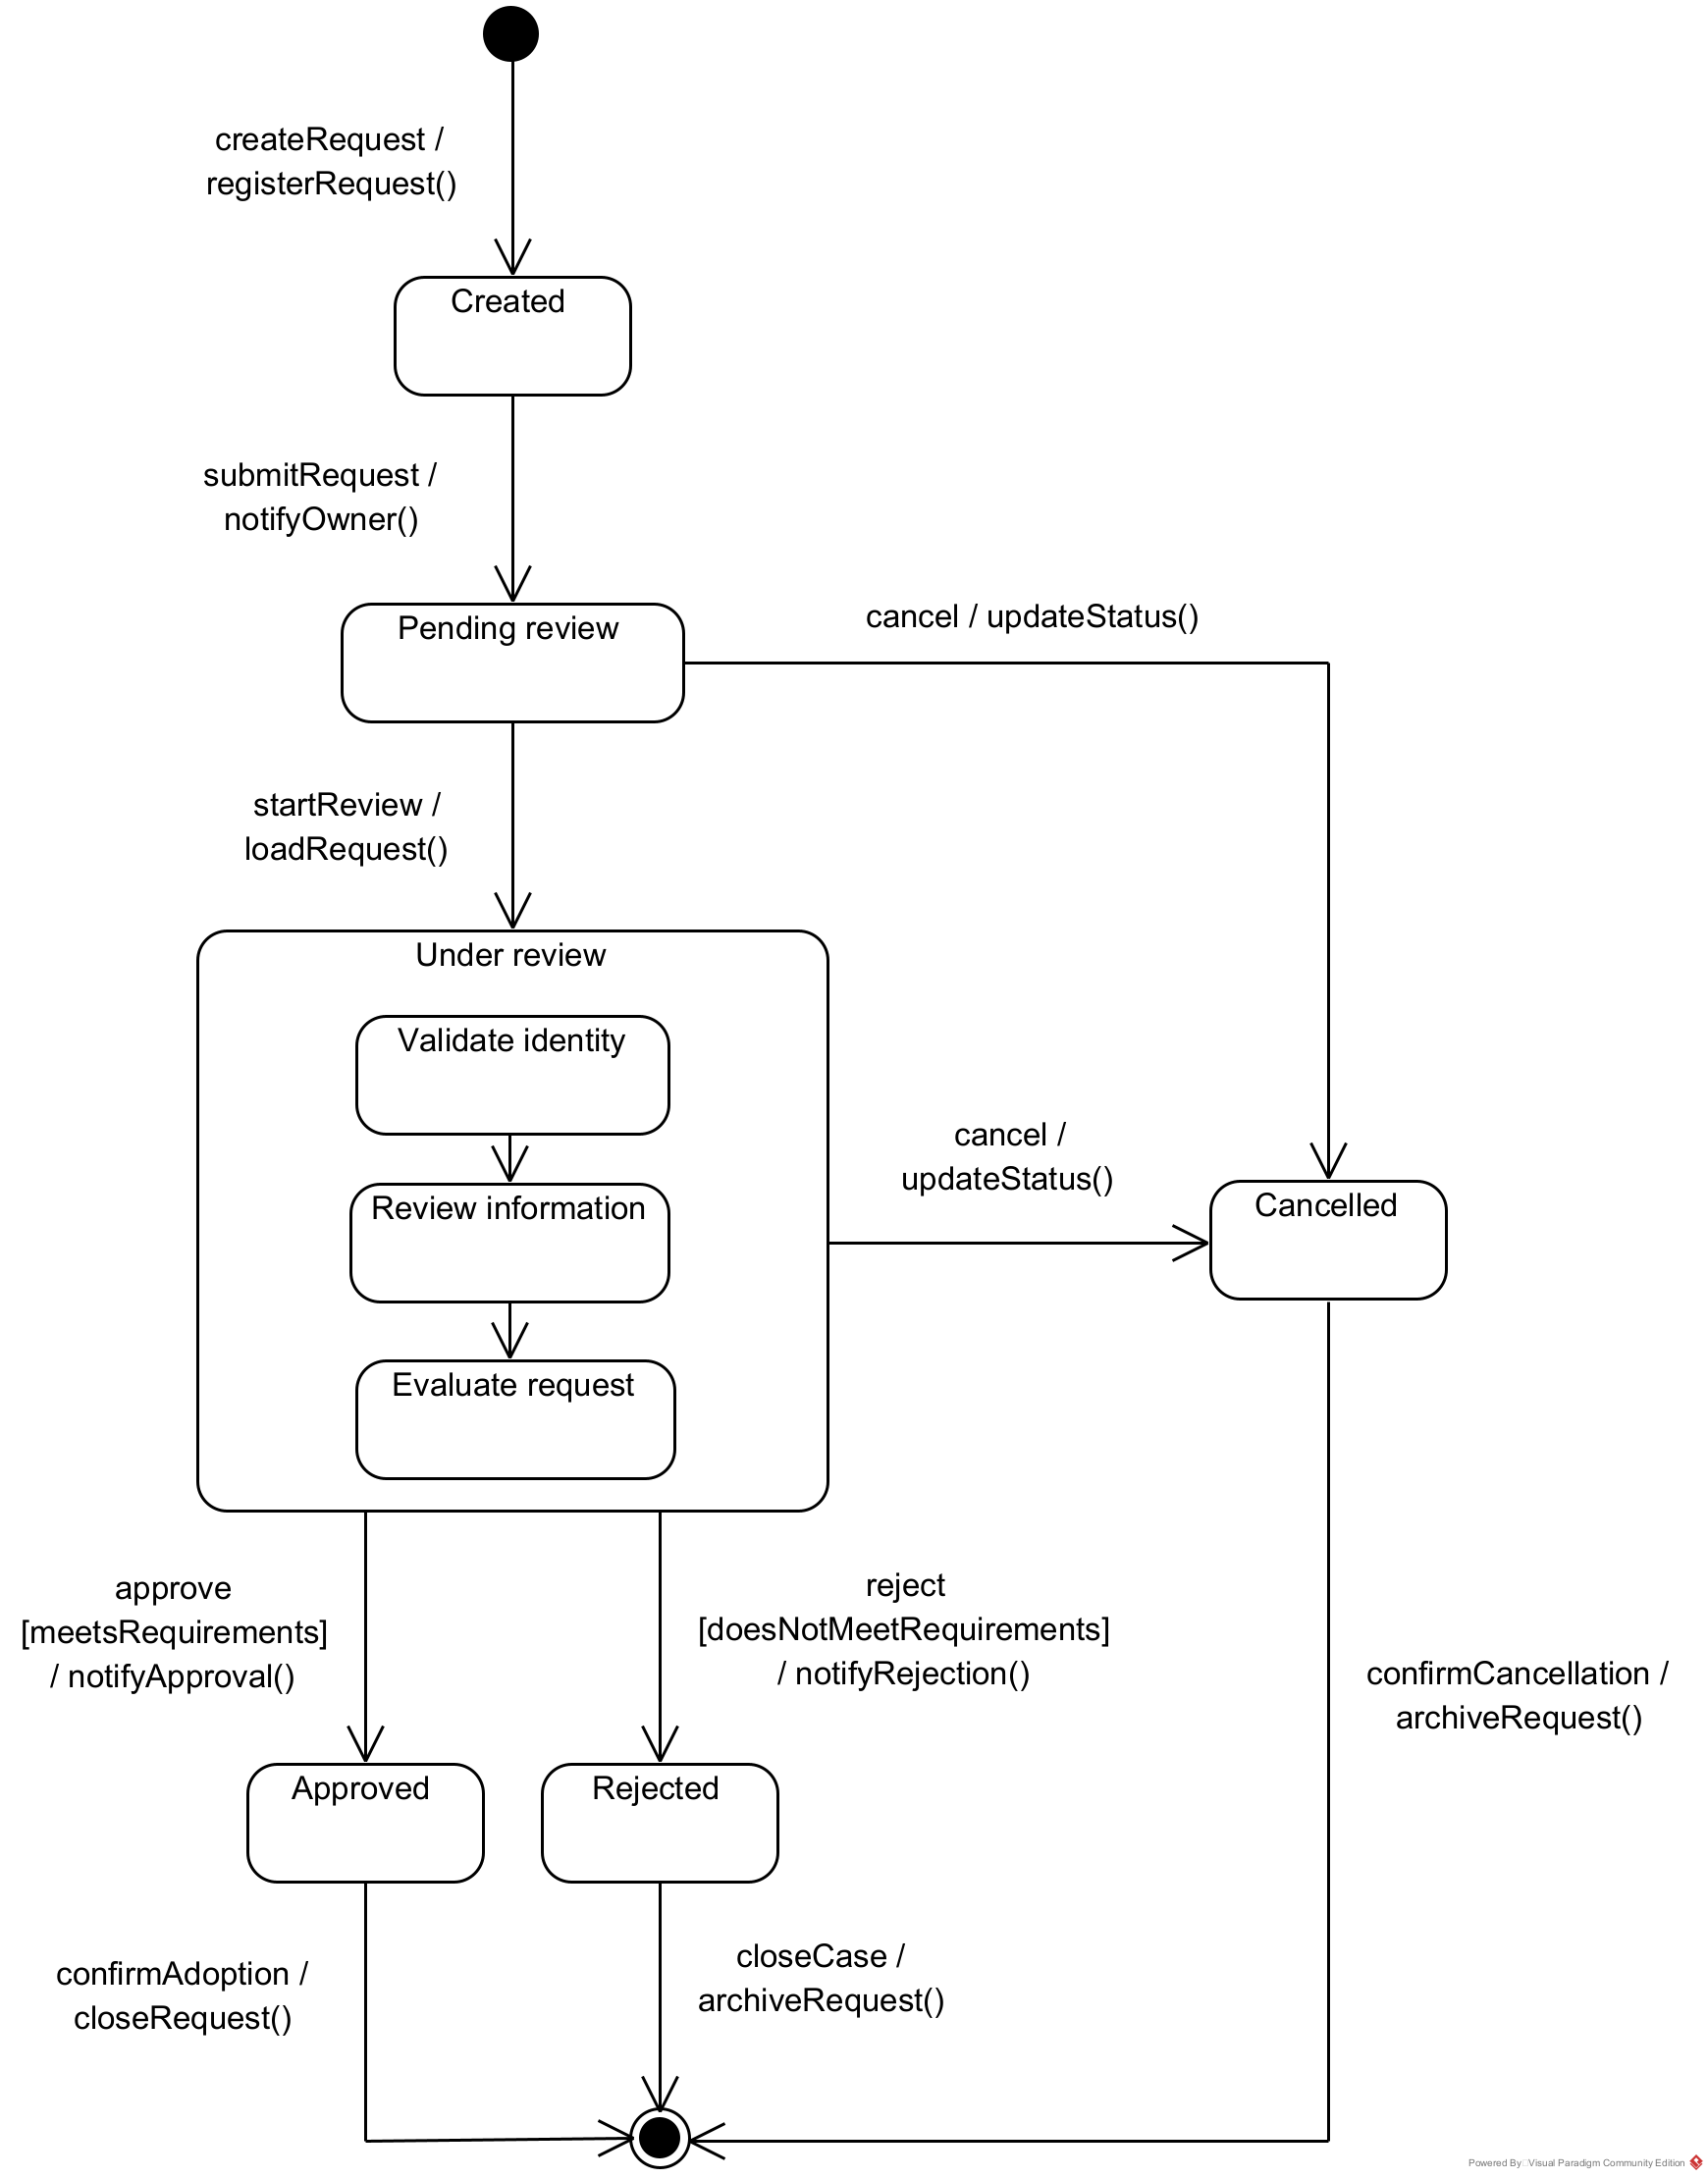
\includegraphics[width=0.79\textwidth]{figuras/DiagramaMaquinasEstado_Solicitudes_MundiPets.png}
		\caption{Diagrama de estados de una solicitud de adopción o cruza.}
		\label{fig:est-solicitud}
	\end{figure}

	\subsubsection{Estados de verificación de documentos médicos}

	La tercera máquina de estados corresponde al ciclo de vida de un
	documento médico cargado por el propietario (carnet de vacunación o
	certificado veterinario), desde su carga inicial en el estado
	\emph{uploaded} (\texttt{storeFile()}) hasta su ingreso, tras asignarse a
	una veterinaria (\texttt{assignVet()}), al estado compuesto
	\emph{Verified}, que verifica secuencialmente \emph{LegibilityChecked},
	\emph{SourceAndDatesVerified} y \emph{VerdictIssued}, en cumplimiento de
	RD-03. Del veredicto emitido, el documento transita a \emph{validated}
	(estado final, si \emph{valid?~=~yes}) o a \emph{rejected} (si
	\emph{valid?~=~no}), notificándose al propietario
	(\texttt{notifyOwner()}); desde \emph{rejected}, el propietario puede
	reenviar el documento (\texttt{resubmitDocument()~/~requeue()}), lo que
	retorna la máquina al estado compuesto \emph{Verified}. La segunda
	validación de RF-26 se registra como un nuevo evento sobre el estado
	\emph{VerdictIssued} ya representado en esta máquina de estados, sin
	reabrir el registro original ni requerir estados o transiciones
	adicionales en la figura.

	\begin{figure}[H]
		\centering
		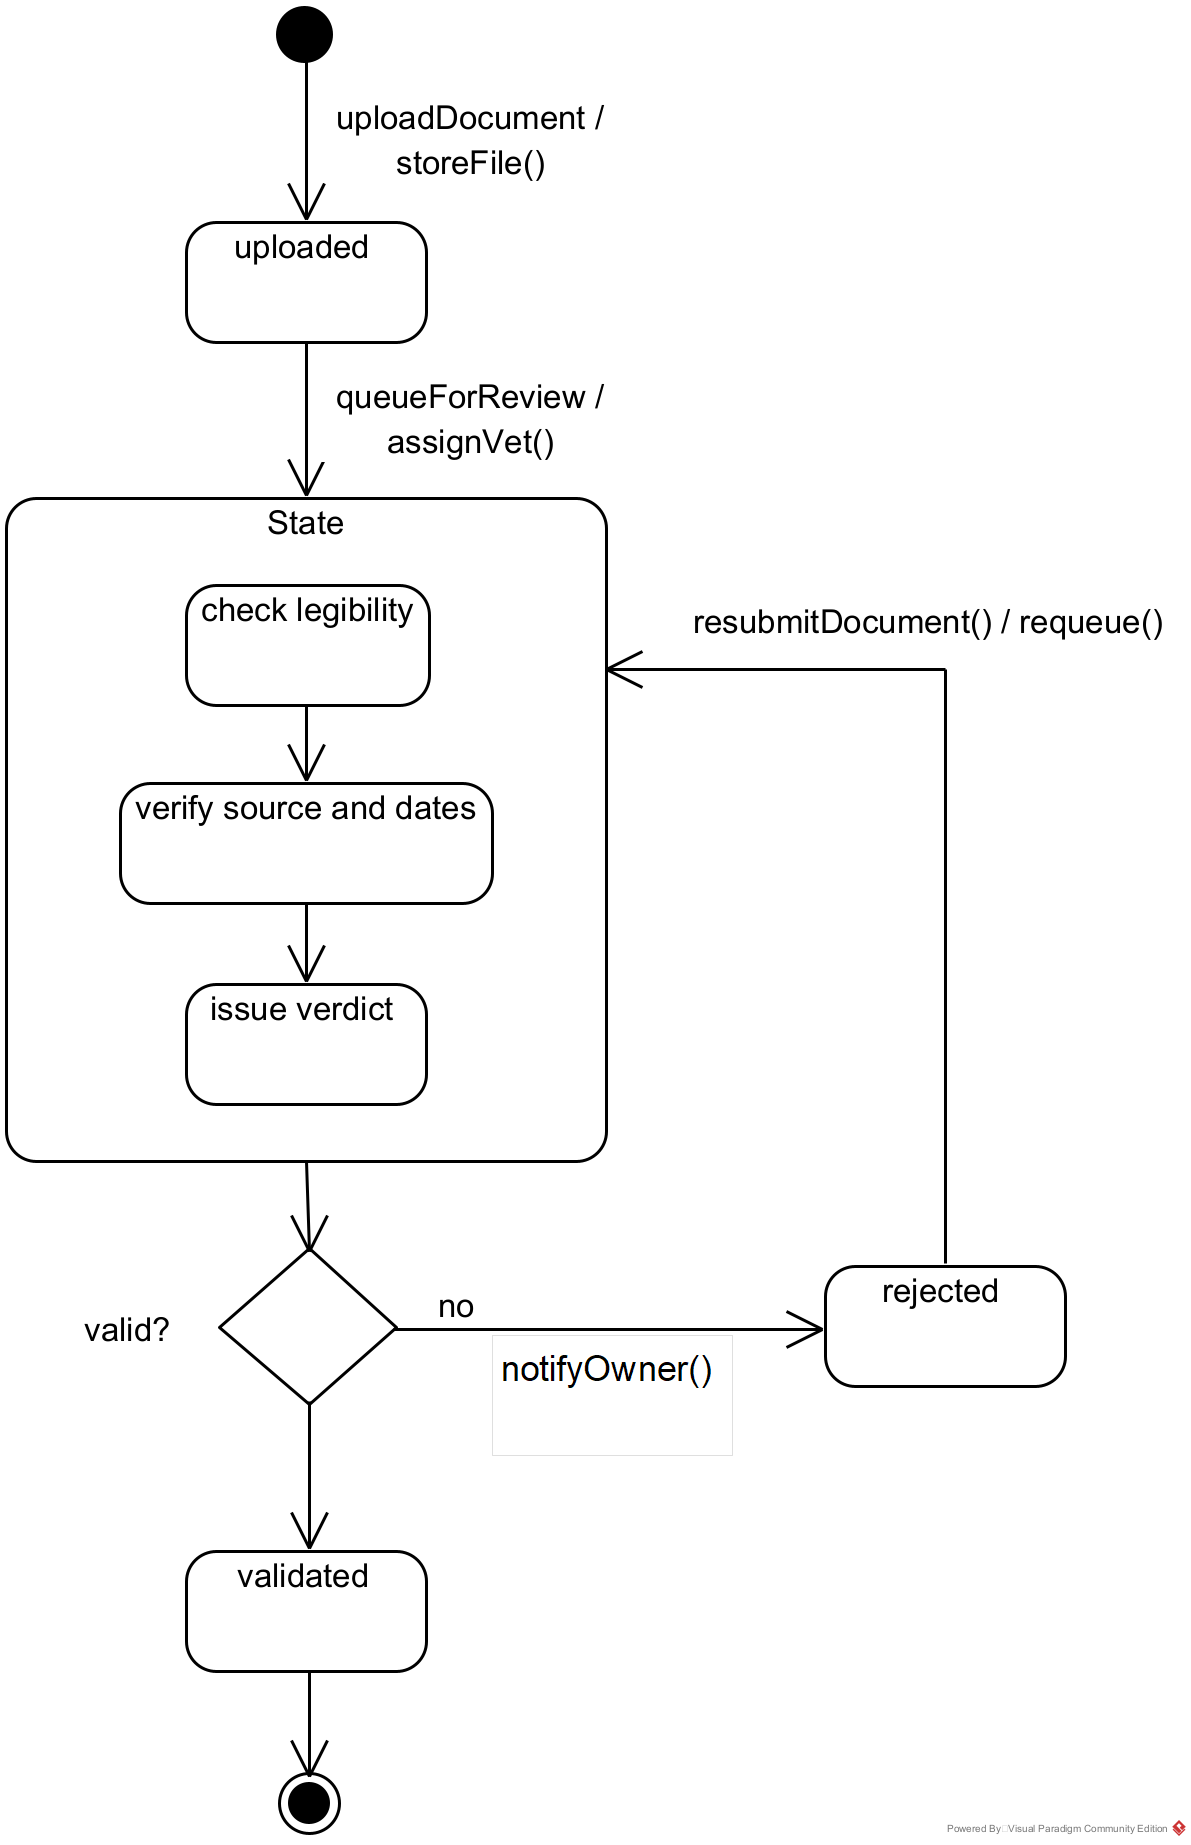
\includegraphics[width=0.65\textwidth]{figuras/DiagramaMaquinasEstado_VerificacionDocumentos_MundiPets.png}
		\caption{Diagrama de estados de verificación de documentos médicos.}
		\label{fig:est-documentos}
	\end{figure}
	
	% ------------------------------------------------------------
	\subsection{Diagrama de componentes}
	\label{sec:componentes}

	El diagrama de componentes traduce la restricción de arquitectura modular
	(RD-05) en una organización concreta de módulos de software con interfaces
	explícitas entre ellos. El \emph{web client} accede al sistema
	exclusivamente a través de la interfaz \texttt{IClientAccess} expuesta por
	la \emph{internal API layer}, que actúa como fachada única y delega en
	tres componentes de dominio mediante sus propias interfaces: \emph{pet
	profiles} (\texttt{IProfile}, RF-01, RF-02, RF-13, RF-16, RF-21, RF-25),
	\emph{request handling} (\texttt{IRequest}, RF-05, RF-08, RF-18, RF-19,
	RF-20, RF-22, RF-27) y \emph{medical validation} (\texttt{IMedical},
	RF-09, RF-14, RF-24, RF-26). Los dos componentes de inteligencia
	artificial se modelan de forma independiente y son consumidos únicamente
	por los componentes de dominio que los necesitan, no directamente por la
	capa de API: \emph{AI image validation} (\texttt{IImageCheck}, RF-17) es
	consumido por \emph{pet profiles}, y \emph{AI compatibility}
	(\texttt{IMatching}, RF-06) es consumido por \emph{request handling}. El
	componente \emph{notifications} (\texttt{IMailer}) es consumido tanto por
	\emph{request handling} como por \emph{medical validation} a través de la
	interfaz común \texttt{INotify}, y persiste hacia un \emph{external mail
	service}; \emph{pet profiles} y \emph{AI compatibility} comparten a su vez
	el acceso a la \emph{relational database} mediante \texttt{IDataAccess}.
	El diagrama no representa un componente de \emph{Mensajería} (RF-07) ni un
	subcomponente de moderación automática de mensajes como elementos
	independientes; ambos quedan implícitos dentro de \emph{request handling}
	y del componente de notificaciones respectivamente.

	Las dependencias entre componentes se limitan a interfaces bien definidas y
	nunca acceden directamente al modelo de datos interno de otro componente:
	tanto \emph{pet profiles} como \emph{AI compatibility} acceden a la base de
	datos relacional a través de la misma interfaz \texttt{IDataAccess} en
	lugar de mantener cada uno su propio acceso, y \emph{request handling}
	notifica a los usuarios a través de \texttt{INotify} sin conocer el
	mecanismo de envío subyacente. Este diseño sustenta directamente la
	métrica de mantenibilidad definida en RNF-10, según la cual una
	modificación en un componente no debería requerir cambios en más del
	10\,\% de los archivos de otro módulo.

	\begin{figure}[H]
		\centering
		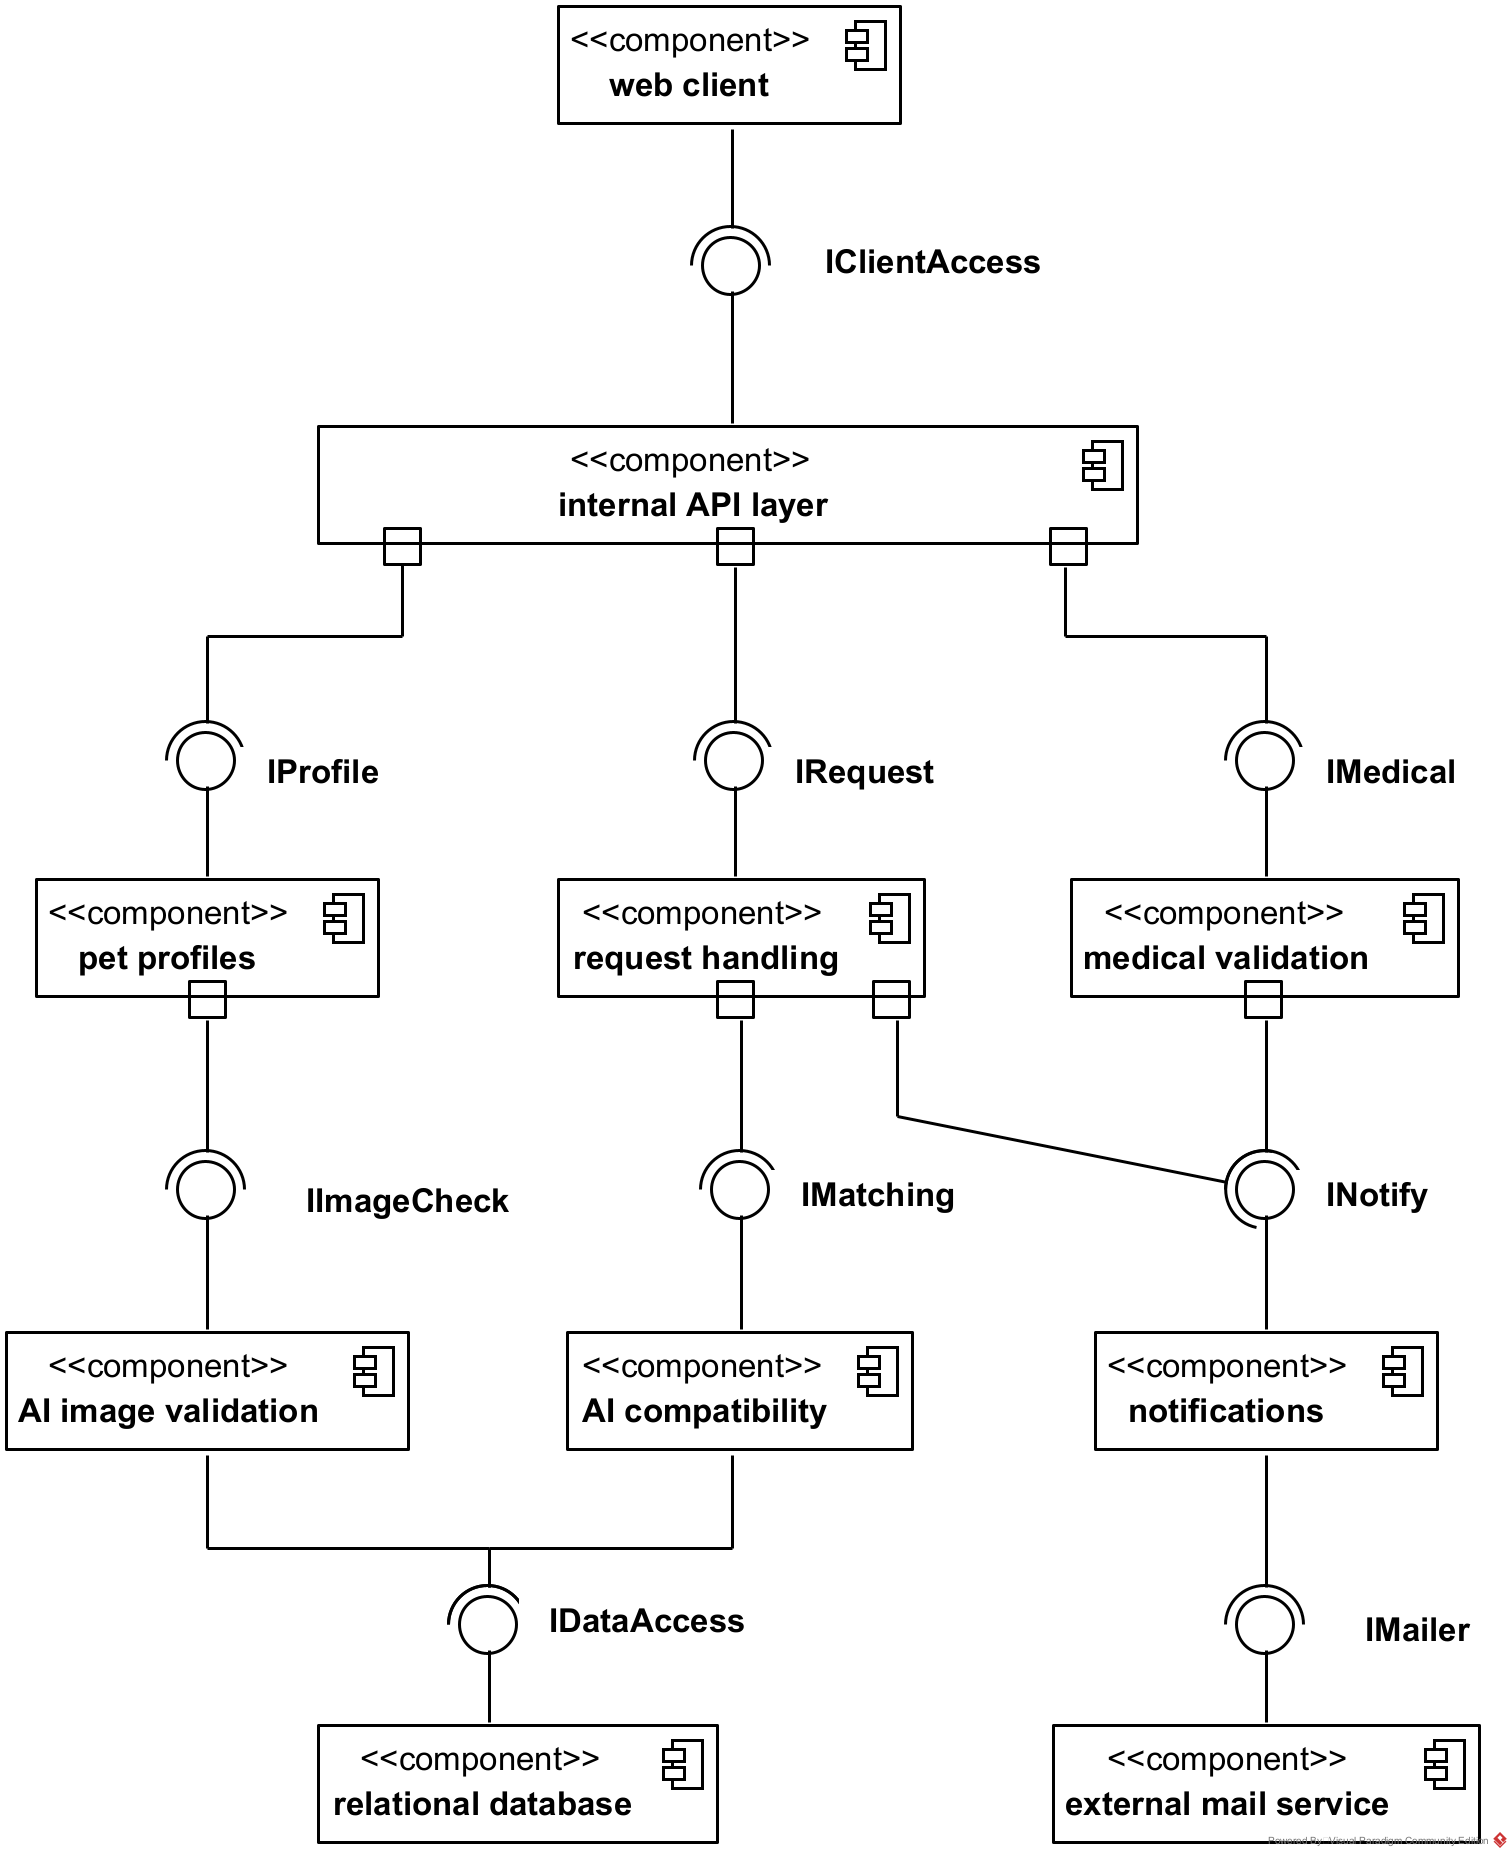
\includegraphics[width=0.75\textwidth]{figuras/DiagramaComponentes_MundiPets.png}
		\caption{Diagrama de componentes del sistema MundiPets.}
		\label{fig:componentes}
	\end{figure}

	% ------------------------------------------------------------
	\subsection{Diagrama de despliegue}
	\label{sec:despliegue}

	El diagrama de despliegue representa la distribución física de los
	componentes del sistema sobre la infraestructura de ejecución, en línea con
	el entorno operativo descrito en la Sección~\ref{sec:entorno}. Se modelan
	dos nodos cliente --- \emph{user workstation} (navegador de escritorio,
	con el requisito de hardware IH-01: Windows o Linux, 4~GB de RAM y 2
	núcleos) y \emph{mobile device} (aplicación móvil empaquetada como
	\texttt{mundipets.apk}, con el requisito IH-02: Android o iOS y 2~GB de
	RAM) --- que acceden mediante HTTPS/REST a un único nodo
	\emph{application server (cloud)}. A diferencia de lo previsto en una
	revisión anterior de este documento, el servidor de aplicaciones no separa
	el componente de inteligencia artificial en un nodo propio: aloja en el
	mismo servidor, junto con los artefactos \texttt{mundipets-api.js} y
	\texttt{mundipets-web.js}, los cuatro componentes \emph{AI compatibility},
	\emph{AI image validation}, \emph{authentication service} y
	\emph{notification module}, bajo el requisito de hardware IH-07 (Linux
	64~bits, 4~vCPU, 8~GB de RAM y 50~GB de disco SSD NVMe).

	Desde el servidor de aplicaciones se conectan tres nodos de persistencia e
	integración externa: el \emph{database server} (artefacto
	\texttt{mundipets\_db}), accedido mediante JDBC/SQL; el \emph{object
	storage}, que persiste los archivos multimedia (fotografías de mascotas y
	documentos veterinarios digitalizados) mediante una API compatible con
	S3; y el \emph{mail server}, accedido mediante SMTP para el envío de
	notificaciones. El diagrama no representa la dependencia hacia la
	WhatsApp Business API descrita en RD-08 y RNF-09 para los recordatorios de
	controles preventivos de RF-10: el canal externo de notificación
	modelado es exclusivamente el correo electrónico (SMTP), por lo que la
	integración con WhatsApp queda pendiente de incorporar en una futura
	versión de este diagrama para que la arquitectura desplegada refleje
	íntegramente lo exigido por RD-08.

	\begin{figure}[H]
		\centering
		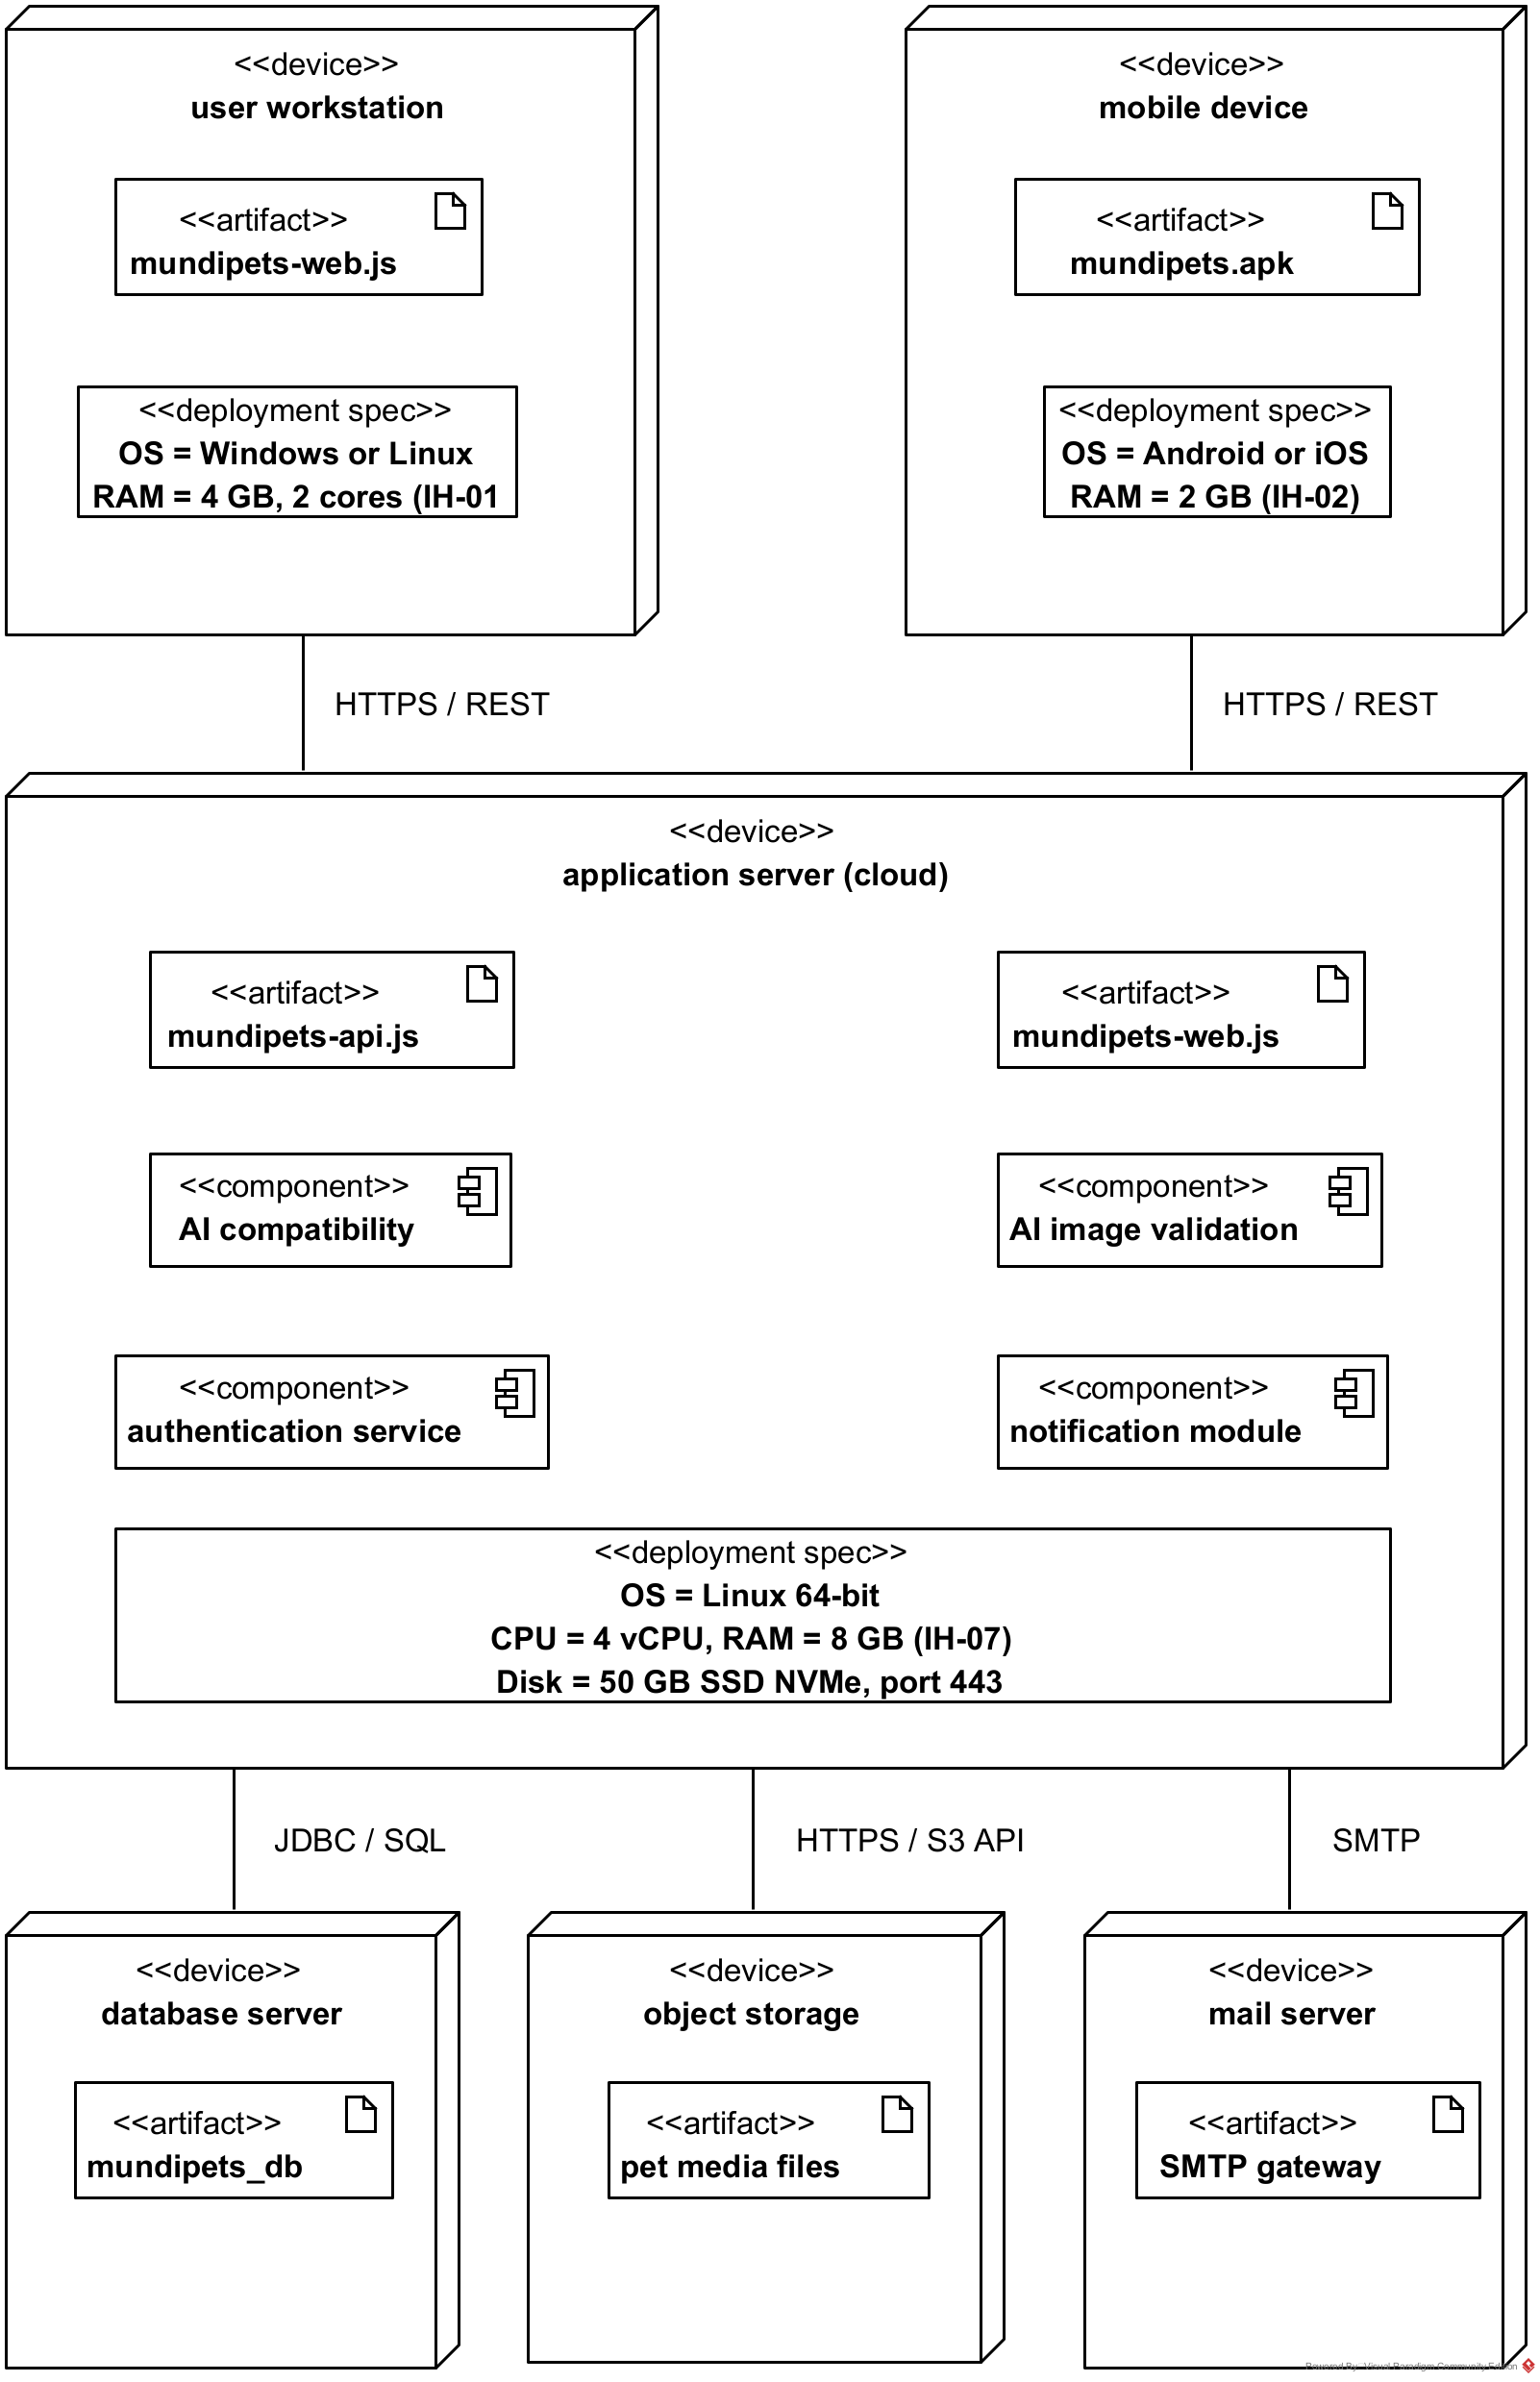
\includegraphics[width=0.65\textwidth]{figuras/DiagramaDespliegue_MundiPets.png}
		\caption{Diagrama de despliegue del sistema MundiPets.}
		\label{fig:despliegue}
	\end{figure}

	% ############################################################
	%        SECCION 5 -- PRIORIZACION Y TRAZABILIDAD EXTENDIDA
	% ############################################################
	\section{Priorización y trazabilidad extendida}
	\label{sec:priorizacion}
	
	\subsection{Clasificación de requisitos}
	\label{sec:clasificacion}
	
	En esta sección se presenta la clasificación general de los requisitos
	definidos para MundiPets, organizándolos según su identificador, nombre y
	tipo. La Tabla~\ref{tab:lista_requisitos_completa} recoge los 61 requisitos
	vigentes de la Entrega 4 (2B): 27 requisitos funcionales (RF-01 a RF-27),
	16 requisitos no funcionales (RNF-01 a RNF-16), 9 restricciones de diseño
	(RD-01 a RD-09) y 9 requisitos legales (RL-01 a RL-09), redactados en las
	Secciones~\ref{sec:rf}, \ref{sec:rnf}, \ref{sec:legales} y
	\ref{sec:restricciones}. Con ello se supera el piso mínimo de 25 RF y 15 RNF
	exigido por esta entrega. RF-26 y RF-27 se incorporan a partir de la nueva
	evidencia recolectada EV-23 (walkthrough/entrevista PROP-12) y EV-24
	(walkthrough/entrevista VET-07). Como cierre de la PE5, el Change Control Board resolvió formalmente
	las 9 RFC pendientes de la inspección PE4 (Sección~\ref{sec:trazabilidad}):
	se corrigen RF-06, RF-07, RF-10, RNF-02 y RNF-03 (RFC-I, RFC-F, RFC-C,
	RFC-E y la corrección de alcance derivada de RFC-G); se redefine el
	alcance de RNF-15 para que sea coherente con RF-07 (RFC-H); y se
	rechazan formalmente, con justificación registrada, la propuesta
	original de RFC-G (relajar el umbral de RNF-03) y las RFC-B y RFC-J por
	no contar con evidencia de entrevista que sustente un requisito
	funcional nuevo y verificable; estas dos últimas quedan documentadas
	como limitaciones de alcance reconocidas en RD-06 y RL-01,
	respectivamente, sin RFC abiertas o sin resolver.
	
	\begin{longtable}{@{}p{2.2cm} p{7.5cm} p{3.5cm}@{}}
		\caption{Clasificación de requisitos y restricciones.}
		\label{tab:lista_requisitos_completa} \\
		\hline
		\textbf{Identificador} & \textbf{Nombre del requisito} & \textbf{Clasificación} \\
		\hline
		\endfirsthead
		\multicolumn{3}{|l|}{\textit{(continuación)}} \\
		\hline
		\textbf{Identificador} & \textbf{Nombre del requisito} & \textbf{Clasificación} \\
		\hline
		\endhead
		\hline
		\endfoot
		RF-01 & Registrar mascota & Requisito funcional \\
		\hline
		RF-02 & Gestionar historial médico de la mascota & Requisito funcional \\
		\hline
		RF-03 & Consultar perfil completo de una mascota & Requisito funcional \\
		\hline
		RF-04 & Buscar y filtrar mascotas & Requisito funcional \\
		\hline
		RF-05 & Gestionar solicitudes de adopción & Requisito funcional \\
		\hline
		RF-06 & Evaluar compatibilidad entre mascotas para cruza & Requisito funcional \\
		\hline
		RF-07 & Sistema de mensajería entre usuarios & Requisito funcional \\
		\hline
		RF-08 & Gestionar solicitudes de cruza & Requisito funcional \\
		\hline
		RF-09 & Validar la información médica de una mascota & Requisito funcional \\
		\hline
		RF-10 & Gestionar recordatorios de controles preventivos & Requisito funcional \\
		\hline
		RF-11 & Administrar la privacidad de la información & Requisito funcional \\
		\hline
		RF-12 & Verificar la identidad de los usuarios & Requisito funcional \\
		\hline
		RF-13 & Registrar publicaciones de mascotas & Requisito funcional \\
		\hline
		RF-14 & Gestionar carnet de vacunación & Requisito funcional \\
		\hline
		RF-15 & Consultar el historial de procesos de adopción y cruza & Requisito funcional \\
		\hline
		RF-16 & Gestionar antecedentes genéticos y parentesco de la mascota & Requisito funcional \\
		\hline
		RF-17 & Validar imágenes & Requisito funcional \\
		\hline
		RF-18 & Gestionar el flujo de solicitud de adopción por etapas & Requisito funcional \\
		\hline
		RF-19 & Validar certificados veterinarios antes de habilitar la cruza & Requisito funcional \\
		\hline
		RF-20 & Coordinar encuentros de socialización supervisados & Requisito funcional \\
		\hline
		RF-21 & Registrar el identificador de microchip de la mascota & Requisito funcional \\
		\hline
		RF-22 & Dar seguimiento post-adopción & Requisito funcional \\
		\hline
		RF-23 & Emitir alertas de riesgo sanitario o físico en interacciones y cruces & Requisito funcional \\
		\hline
		RF-24 & Registrar trazabilidad de cepa, lote y aplicador de cada vacuna & Requisito funcional \\
		\hline
		RF-25 & Publicar aviso de mascota extraviada & Requisito funcional \\
		\hline
		RF-26 & Habilitar validación médica por segunda opinión veterinaria & Requisito funcional \\
		\hline
		RF-27 & Controlar y alertar sobre solicitudes repetitivas de cruza de una misma mascota & Requisito funcional \\
		\hline
		RNF-01 & Protección de la información de propietarios y mascotas & Requisito no funcional \\
		\hline
		RNF-02 & Disponibilidad del sistema & Requisito no funcional \\
		\hline
		RNF-03 & Tiempo de respuesta del sistema & Requisito no funcional \\
		\hline
		RNF-04 & Facilidad de uso de la plataforma & Requisito no funcional \\
		\hline
		RNF-05 & Integridad de la información médica & Requisito no funcional \\
		\hline
		RNF-06 & Exactitud del componente de inteligencia artificial & Requisito no funcional \\
		\hline
		RNF-07 & Precisión en la validación de imágenes & Requisito no funcional \\
		\hline
		RNF-08 & Actualización de la información registrada & Requisito no funcional \\
		\hline
		RNF-09 & Interoperabilidad de notificaciones con canales externos & Requisito no funcional \\
		\hline
		RNF-10 & Facilidad de mantenimiento del código & Requisito no funcional \\
		\hline
		RNF-11 & Portabilidad entre navegadores y dispositivos & Requisito no funcional \\
		\hline
		RNF-12 & Escalabilidad ante crecimiento de usuarios & Requisito no funcional \\
		\hline
		RNF-13 & Explicabilidad de la recomendación de compatibilidad para cruza & Requisito no funcional \\
		\hline
		RNF-14 & Explicabilidad del rechazo o aceptación de imágenes & Requisito no funcional \\
		\hline
		RNF-15 & Explicabilidad de la moderación de mensajes & Requisito no funcional \\
		\hline
		RNF-16 & Confidencialidad de datos de ubicación y contacto & Requisito no funcional \\
		\hline
		RD-01 & Integración de componentes de inteligencia artificial & Restricción de diseño \\
		\hline
		RD-02 & Acceso basado en roles & Restricción de diseño \\
		\hline
		RD-03 & Validación profesional de la información médica & Restricción de diseño \\
		\hline
		RD-04 & Protección de datos personales & Restricción de diseño \\
		\hline
		RD-05 & Arquitectura modular del sistema & Restricción de diseño \\
		\hline
		RD-06 & Mecanismo de eliminación de cuenta y datos personales & Restricción de diseño \\
		\hline
		RD-07 & Protocolo de notificación de vulneraciones de seguridad & Restricción de diseño \\
		\hline
		RD-08 & Dependencia de servicios externos de mensajería & Restricción de diseño \\
		\hline
		RD-09 & Anonimización de evidencias de campo para publicación abierta & Restricción de diseño \\
		\hline
		RL-01 & Consentimiento libre, específico, informado e inequívoco & Requisito legal \\
		\hline
		RL-02 & Información de finalidad y derecho de acceso & Requisito legal \\
		\hline
		RL-03 & Derecho de rectificación y actualización & Requisito legal \\
		\hline
		RL-04 & Derecho de supresión de datos personales & Requisito legal \\
		\hline
		RL-05 & Minimización y seguridad de los datos & Requisito legal \\
		\hline
		RL-06 & Derecho a explicación de decisiones automatizadas & Requisito legal \\
		\hline
		RL-07 & Confidencialidad reforzada de datos sensibles y de salud & Requisito legal \\
		\hline
		RL-08 & Protección de datos desde el diseño y por defecto & Requisito legal \\
		\hline
		RL-09 & Notificación de vulneraciones de seguridad & Requisito legal \\
	\end{longtable}
	
	\newpage
	
	\subsection{Priorización MoSCoW}
	\label{sec:moscow}
	
	La Tabla~\ref{tab:priorizacion_moscow_parcial} presenta la priorización
	MoSCoW extendida de los 61 requisitos vigentes del proyecto, actualizando y
	ampliando la clasificación heredada de la Entrega 2 (1B) con los
	identificadores incorporados en entregas previas (RF-18 a RF-25, RNF-09 a
	RNF-16, RD-06 a RD-09 y RL-01 a RL-09) y con RF-26 y RF-27, incorporados en
	la presente revisión (4.0). La misma priorización, junto con su
	clasificación Kano y su valor WSJF, se consolida en el
	\textbf{\hyperref[tab:priorizacion_moscow_completa]{Apéndice C --- Priorización
			MoSCoW, Kano y WSJF (detalle)}}.
	
	\begin{longtable}{@{}p{1.6cm} p{4.8cm} p{1.6cm} p{5.2cm}@{}}
		\caption{Priorización MoSCoW extendida.}
		\label{tab:priorizacion_moscow_parcial} \\
		\hline
		\textbf{ID} & \textbf{Requisito} & \textbf{Prioridad} & \textbf{Justificación} \\
		\hline
		\endfirsthead
		\multicolumn{4}{|l|}{\textit{(continuación)}} \\
		\hline
		\textbf{ID} & \textbf{Requisito} & \textbf{Prioridad} & \textbf{Justificación} \\
		\hline
		\endhead
		\hline
		\endfoot
		RF-01 & Registrar mascota & Must & Es el pilar del sistema; sin este RF no puede existir ningún perfil de mascota ni proceso posterior. \\
		\hline
		RF-02 & Gestionar historial médico & Must & Crítico para la salud animal y para RL-03 (rectificación de datos médicos). \\
		\hline
		RF-03 & Consultar perfil completo & Must & Fundamental para que adoptantes e interesados en cruza tomen decisiones informadas; sustenta RL-02. \\
		\hline
		RF-04 & Buscar y filtrar mascotas & Should & Mejora la usabilidad, pero el sistema puede operar inicialmente con listas generales. \\
		\hline
		RF-05 & Gestionar solicitudes de adopción & Must & Núcleo del modelo operativo de la plataforma. \\
		\hline
		RF-06 & Evaluar compatibilidad para cruza & Must & Requisito diferenciador que usa IA; motivó RD-01 y exige la explicabilidad de RL-06. \\
		\hline
		RF-07 & Sistema de mensajería & Could & Deseable para coordinar procesos, pero el contacto inicial puede derivarse a canales externos si hay limitaciones de tiempo. \\
		\hline
		RF-08 & Gestionar solicitudes de cruza & Must & Operación central del modelo de negocio junto a RF-05. \\
		\hline
		RF-09 & Validar información médica & Must & Imprescindible para la confiabilidad clínica del sistema. \\
		\hline
		RF-10 & Recordatorios de controles preventivos & Should & Aporta valor de bienestar animal, pero no bloquea el flujo principal de adopciones. \\
		\hline
		RF-11 & Administrar privacidad & Must & Mandatorio por RL-02 y RL-05; es el RF más citado en las entrevistas (9 EV). \\
		\hline
		RF-12 & Verificar identidad de usuarios & Must & Indispensable para evitar fraude; sustenta el consentimiento de RL-01. \\
		\hline
		RF-13 & Registrar publicaciones & Must & Necesario para que un propietario active la disponibilidad de su mascota. \\
		\hline
		RF-14 & Gestionar carnet de vacunación & Must & Crítico para la trazabilidad sanitaria; sustenta RL-03. \\
		\hline
		RF-15 & Consultar historial de procesos & Could & Aporta trazabilidad al usuario, pero no es indispensable para completar una adopción o cruza. \\
		\hline
		RF-16 & Antecedentes genéticos y parentesco & Must & Necesario para que RF-06 pueda evaluar compatibilidad de forma responsable. \\
		\hline
		RF-17 & Validar imágenes con IA & Should & Refuerza la seguridad del contenido, pero el sistema puede operar con moderación manual inicial. \\
		\hline
		RF-18 & Flujo de adopción por etapas & Must & Formaliza el proceso de adopción responsable identificado en la segunda ronda de campo (EV-11, EV-16). \\
		\hline
		RF-19 & Validar certificados veterinarios antes de cruza & Should & Refuerza la confiabilidad de RF-06, pero no bloquea su funcionamiento básico. \\
		\hline
		RF-20 & Encuentros de socialización supervisados & Could & Valor deseable de bienestar animal, mencionado por un solo participante (EV-13). \\
		\hline
		RF-21 & Registrar identificador de microchip & Should & Aporta trazabilidad complementaria al carnet de vacunación. \\
		\hline
		RF-22 & Seguimiento post-adopción & Must & Cierra el ciclo de responsabilidad de RF-18, exigido por participantes de la segunda ronda. \\
		\hline
		RF-23 & Alertas de riesgo sanitario o físico & Must & Mitiga un riesgo real de seguridad y salud animal detectado en varias entrevistas (EV-09, EV-12, EV-15, EV-18). \\
		\hline
		RF-24 & Trazabilidad de cepa, lote y aplicador & Should & Complementa RF-14 con datos adicionales de trazabilidad, no bloqueante. \\
		\hline
		RF-25 & Aviso de mascota extraviada & Could & Funcionalidad de valor social, pero fuera del núcleo de adopción/cruza del sistema. \\
		\hline
		RF-26 & Segunda opinión veterinaria & Should & Refuerza la confiabilidad clínica mediante revisión entre pares; la veterinaria entrevistada (EV-24) la identificó como la mejora que más valor le aportaría, aunque no bloquea la validación individual ya cubierta por RF-09. \\
		\hline
		RF-27 & Control de cruzas repetitivas & Should & Mitiga un riesgo de maltrato animal identificado explícitamente por la propietaria entrevistada (EV-23) al validar RF-14 y en la síntesis final del walkthrough; no bloquea el flujo de solicitud de cruza ya cubierto por RF-08. \\
		\hline
		RNF-01 & Protección de información de propietarios y mascotas & Must & Requisito estricto de seguridad; sustenta RL-05 y RL-07. \\
		\hline
		RNF-02 & Disponibilidad del sistema & Must & Crítico para la operatividad continua de la plataforma. \\
		\hline
		RNF-03 & Tiempo de respuesta del sistema & Should & Mejora la experiencia, pero el sistema es funcional con tiempos mayores en una primera versión. \\
		\hline
		RNF-04 & Facilidad de uso de la plataforma & Should & Relevante para adopción del producto, pero no bloquea sus funciones. \\
		\hline
		RNF-05 & Integridad de la información médica & Must & Evita modificaciones no autorizadas del historial clínico; sustenta RL-07. \\
		\hline
		RNF-06 & Exactitud del componente de IA & Must & Sin una precisión mínima, RF-06 pierde su valor diferenciador. \\
		\hline
		RNF-07 & Precisión en validación de imágenes & Should & Mejora la calidad del contenido, pero RF-17 puede operar con una tasa de error inicial mayor. \\
		\hline
		RNF-08 & Actualización de la información registrada & Should & Mejora la confianza del usuario, no bloquea el flujo principal. \\
		\hline
		RNF-09 & Interoperabilidad de notificaciones & Should & Aporta valor (recordatorios por WhatsApp), pero el sistema opera sin ella mediante notificación interna. \\
		\hline
		RNF-10 & Facilidad de mantenimiento del código & Should & Importante para sostenibilidad técnica, pero no bloquea la operación funcional del MVP. \\
		\hline
		RNF-11 & Portabilidad entre navegadores & Should & Necesaria para alcance de usuarios, pero el sistema puede operar inicialmente en un navegador principal. \\
		\hline
		RNF-12 & Escalabilidad ante crecimiento de usuarios & Could & Deseable a mediano plazo; no crítica mientras la base de usuarios sea reducida. \\
		\hline
		RNF-13 & Explicabilidad de compatibilidad para cruza & Must & Exigido por el derecho legal a explicación (RL-06) sobre decisiones automatizadas del RF-06. \\
		\hline
		RNF-14 & Explicabilidad de rechazo de imágenes & Should & Mejora la confianza del usuario, pero el sistema puede operar con un mensaje de rechazo genérico inicialmente. \\
		\hline
		RNF-15 & Explicabilidad de moderación de mensajes & Should & Igual que RNF-14: deseable para confianza, no bloqueante. \\
		\hline
		RNF-16 & Confidencialidad de ubicación y contacto & Must & Obligación legal directa (RL-05, principio de minimización). \\
		\hline
		RD-01 & Integración de componentes de IA & Must & Restricción ineludible: arquitectura del principal valor agregado de MundiPets. \\
		\hline
		RD-02 & Acceso basado en roles & Must & Mandatorio para diferenciar permisos de propietarios, veterinarias y administradores; sustenta RL-05 y RL-08. \\
		\hline
		RD-03 & Validación profesional de la información médica & Must & Exigido por los veterinarios entrevistados para garantizar confiabilidad clínica. \\
		\hline
		RD-04 & Protección de datos personales & Must & Implementa directamente RL-05, RL-07 y RL-08. \\
		\hline
		RD-05 & Arquitectura modular del sistema & Must & Facilita mantenimiento e incorporación de nuevas funcionalidades; sustenta RNF-10. \\
		\hline
		RD-06 & Eliminación de cuenta y datos personales & Must & Obligación legal ineludible (RL-04, derecho de supresión); sin este mecanismo el sistema incumple la LOPDP. \\
		\hline
		RD-07 & Protocolo de notificación de vulneraciones & Must & Exigido por RL-09 con plazos legales estrictos (5 y 3 días). \\
		\hline
		RD-08 & Dependencia de servicios externos de mensajería & Should & Aporta valor (RF-10) pero requiere un canal de respaldo ante caídas del proveedor. \\
		\hline
		RD-09 & Anonimización de evidencias para publicación abierta & Must & Exigido por los Art. 30-32 LOPDP para el uso de datos de investigación en el paquete FAIR. \\
		\hline
		RL-01 & Consentimiento libre, específico, informado e inequívoco & Must & Toda obligación legal es no negociable: su incumplimiento expone al proyecto a responsabilidad legal. \\
		\hline
		RL-02 & Información de finalidad y derecho de acceso & Must & Ídem: obligación legal directa (Art. 12-13 LOPDP). \\
		\hline
		RL-03 & Derecho de rectificación y actualización & Must & Ídem: obligación legal directa (Art. 14 LOPDP). \\
		\hline
		RL-04 & Derecho de supresión de datos personales & Must & Ídem: obligación legal directa (Art. 15 LOPDP). \\
		\hline
		RL-05 & Minimización y seguridad de los datos & Must & Ídem: obligación legal directa (Art. 10 LOPDP). \\
		\hline
		RL-06 & Derecho a explicación de decisiones automatizadas & Must & Ídem: obligación legal directa (Art. 20 LOPDP); base de todo el bloque de explicabilidad. \\
		\hline
		RL-07 & Confidencialidad reforzada de datos sensibles y de salud & Must & Ídem: obligación legal directa (Art. 25-30 LOPDP). \\
		\hline
		RL-08 & Protección de datos desde el diseño y por defecto & Must & Ídem: obligación legal directa (Art. 39 LOPDP). \\
		\hline
		RL-09 & Notificación de vulneraciones de seguridad & Must & Ídem: obligación legal directa (Art. 43 y 46 LOPDP), con plazos estrictos. \\
	\end{longtable}
	
	\textbf{Justificación de Must/Won't}
	
	\textbf{Must Have} \\
	Los requisitos clasificados como Must Have corresponden a funcionalidades
	indispensables para el funcionamiento del sistema, tales como el registro de
	mascotas, la gestión del historial médico, la autenticación de usuarios y la
	evaluación de compatibilidad para cruza mediante inteligencia artificial. La
	ausencia de cualquiera de estos requisitos impediría cumplir los objetivos
	principales del proyecto.
	
	\textbf{Won't Have} \\
	En la presente versión del proyecto no se identificaron requisitos
	clasificados como Won't Have, ya que todos los requisitos levantados fueron
	considerados necesarios (Must), importantes (Should) o deseables (Could) para
	el alcance definido. Por ello, no existen funcionalidades descartadas
	explícitamente para futuras versiones.
	
	\subsection{Modelo de Kano}
	\label{sec:kano}
	
	\paragraph{Alcance y limitación del instrumento.}
	El modelo de Kano \cite{kano1984} clasifica los atributos de un producto en
	básicos, de desempeño, de deleite, indiferentes o de rechazo a partir de un
	par de preguntas por atributo: una \emph{funcional} (cómo se sentiría la
	persona usuaria si el sistema ofreciera el atributo) y una
	\emph{disfuncional} (cómo se sentiría si no lo ofreciera). La categoría se
	obtiene cruzando ambas respuestas en la matriz de evaluación del modelo.
	
	El cuestionario v2.0 aplicado en la segunda ronda de campo midió la
	\textbf{importancia declarada} de cada atributo en una escala Likert de 1 a
	5, pero \textbf{no incluyó el par funcional/disfuncional}. En consecuencia,
	\textbf{no es posible derivar una clasificación Kano canónica a partir de
		los datos primarios disponibles}. Declarar categorías Kano sobre estos datos
	sería atribuir al instrumento una medición que no realizó.
	
	Lo que sí permite el instrumento es un ordenamiento por importancia
	declarada, que se reporta a continuación como \textbf{aproximación} y que
	\textbf{no constituye una clasificación Kano}. Se usa como insumo
	complementario de la priorización MoSCoW (Sección~\ref{sec:moscow}) y del
	cálculo WSJF (Sección~\ref{sec:wsjf}), no como sustituto del modelo.
	
	\paragraph{Resultados de importancia declarada.}
	La Tabla~\ref{tab:importancia-declarada} presenta la media, el porcentaje de
	personas que asignaron la calificación máxima y la desviación estándar de
	cada atributo, sobre $n = 61$ respuestas válidas del cuestionario v2.0
	(47 del perfil dominante \emph{propietario de mascota}, 7 de
	\emph{interesado en adopción} y 7 de \emph{interesado en cruza}).
	
	\begin{table}[H]
		\centering
		\caption[Importancia declarada de los atributos (aproximación, no Kano)]{Importancia declarada de los atributos del sistema. \textbf{Aproximación basada en escala Likert; no constituye clasificación Kano.}}
		\label{tab:importancia-declarada}
		\small
		\begin{tabularx}{\textwidth}{@{}l X c c c c@{}}
			\toprule
			\textbf{ID} & \textbf{Atributo evaluado} & \textbf{RF/RNF} & \textbf{Media} & \textbf{\% máx.} & \textbf{DE} \\
			\midrule
			IM-01 & Registro del historial de vacunación & RF-14, RF-24 & 4,67 & 82,0 & 0,83 \\
			IM-02 & Validación de la información médica por veterinaria & RF-09, RD-03 & 4,69 & 77,0 & 0,65 \\
			IM-03 & Registro de enfermedades y condiciones previas & RF-02 & 4,64 & 77,0 & 0,75 \\
			IM-04 & Registro de desparasitaciones & RF-02 & 4,62 & 73,8 & 0,76 \\
			IM-05 & Evaluación de compatibilidad para cruza & RF-06 & 4,51 & 62,3 & 0,70 \\
			IM-06 & Conocer la edad de la mascota & RF-01, RF-03 & 4,43 & 59,0 & 0,83 \\
			IM-07 & Verificación de identidad de los usuarios & RF-12 & 4,41 & 57,4 & 0,80 \\
			IM-08 & Filtros de búsqueda por edad, raza o ubicación & RF-04 & 4,21 & 45,9 & 0,86 \\
			IM-09 & Fotografías actualizadas de la mascota & RF-01, RF-03 & 4,05 & 36,1 & 0,92 \\
			IM-10 & Sistema de mensajería entre usuarios & RF-07 & 3,98 & 32,8 & 0,88 \\
			IM-11 & Conocer la raza de la mascota & RF-01, RF-03 & 3,92 & 42,6 & 1,20 \\
			\bottomrule
		\end{tabularx}
	\end{table}
	
	\paragraph{Lectura de los resultados.}
	Los cuatro atributos de mayor importancia (IM-01 a IM-04) corresponden todos
	al bloque de información clínica de la mascota y concentran entre el 73\,\%
	y el 82\,\% de calificaciones máximas, con desviaciones estándar por debajo
	de 0,85. Ese patrón de consenso alto y dispersión baja es coherente con
	atributos cuya ausencia se percibe como un defecto del producto, y respalda
	la clasificación \emph{Must have} que ya reciben en MoSCoW.
	
	En el extremo opuesto, la mensajería entre usuarios (IM-10) y las
	fotografías actualizadas (IM-09) obtienen menos del 37\,\% de calificación
	máxima, y el atributo raza (IM-11) presenta la mayor dispersión de todo el
	instrumento ($DE = 1{,}20$), lo que indica desacuerdo real entre perfiles y
	no indiferencia generalizada. Estos tres atributos se mantienen como
	\emph{Should have} o \emph{Could have}.
	
	\paragraph{Nota metodológica sobre el alcance de esta clasificación.}
	La clasificación presentada en esta sección es una aproximación basada en
	importancia declarada de un solo factor, y no una clasificación Kano en
	sentido estricto, la cual exige el par de preguntas funcional y
	disfuncional con las cinco opciones de respuesta del modelo para cada
	atributo de la Tabla~\ref{tab:importancia-declarada}. Esta decisión de
	alcance se declara explícitamente como limitación del diseño empírico en
	la Sección~\ref{sec:amenazas}, de modo que el resultado se lea como lo que
	es --- un proxy razonado de importancia relativa --- y no se presente como
	una clasificación Kano completa que el instrumento v2.0 no estaba
	diseñado para producir. RF-26 y RF-27, incorporados en la presente
	revisión (4.0) a partir de EV-23 y EV-24, se recolectaron con
	posterioridad al cuestionario v2.0 y por ello no cuentan con dato de
	importancia declarada; su priorización se sustenta en MoSCoW
	(Sección~\ref{sec:moscow}) y en WSJF (Sección~\ref{sec:wsjf}), ambos
	aplicados de manera directa a partir de la evidencia de campo EV-23 y
	EV-24, sin depender del instrumento cuantitativo.
	
	\subsection{Valor de negocio con WSJF}
	\label{sec:wsjf}
	
	La técnica WSJF (\emph{Weighted Shortest Job First}) ordena el trabajo
	pendiente según la relación entre el costo del retraso y el tamaño estimado
	del trabajo, siguiendo la fórmula:
	\[
	\mathrm{WSJF} = \frac{\text{Valor de negocio} + \text{Criticidad temporal} + \text{Reducción de riesgo}}{\text{Tamaño del trabajo}}
	\]
	Los cuatro factores se estiman en equipo con la sucesión de Fibonacci
	modificada (1, 2, 3, 5, 8, 13, 20).
	
	El equipo estimó los cuatro factores de WSJF para los 23 RF de prioridad
	\emph{Must} y \emph{Should} —incluyendo RF-26 y RF-27, incorporados en la
	presente revisión (4.0)—, apoyándose en evidencia ya disponible para
	reducir la arbitrariedad de la estimación: el número de evidencias (EV) que
	respaldan cada RF (Apéndice B.1) como indicador de valor de negocio, y la
	existencia de una obligación legal asociada (RL, Sección \ref{sec:legales})
	como indicador de criticidad temporal. Los RF de prioridad \emph{Could}
	(RF-07, RF-15, RF-20, RF-25) se excluyeron del ejercicio por ser ya la
	prioridad más baja de MoSCoW.
	
	\begin{longtable}{@{}p{1.4cm} p{5.4cm} p{1.5cm} p{1.5cm} p{1.5cm} p{1.5cm} p{1.3cm}@{}}
		\caption{Ranking WSJF de los RF \emph{Must} y \emph{Should} de MundiPets.}
		\label{tab:wsjf} \\
		\hline
		\textbf{ID-RF} & \textbf{Nombre} & \textbf{Valor} & \textbf{Criticidad} & \textbf{Riesgo} & \textbf{Tamaño} & \textbf{WSJF} \\
		\hline
		\endfirsthead
		\multicolumn{7}{|l|}{\textit{(continuación)}} \\
		\hline
		\textbf{ID-RF} & \textbf{Nombre} & \textbf{Valor} & \textbf{Criticidad} & \textbf{Riesgo} & \textbf{Tamaño} & \textbf{WSJF} \\
		\hline
		\endhead
		\hline
		\endfoot
		RF-01 & Registrar mascota & 20 & 13 & 13 & 5 & \textbf{9,20} \\
		\hline
		RF-03 & Consultar perfil completo & 13 & 8 & 5 & 3 & \textbf{8,67} \\
		\hline
		RF-13 & Registrar publicaciones de mascotas & 13 & 5 & 3 & 3 & \textbf{7,00} \\
		\hline
		RF-12 & Verificar identidad de usuarios & 8 & 8 & 13 & 5 & \textbf{5,80} \\
		\hline
		RF-11 & Administrar privacidad de la información & 20 & 13 & 13 & 8 & \textbf{5,75} \\
		\hline
		RF-09 & Validar información médica & 8 & 5 & 8 & 5 & \textbf{4,20} \\
		\hline
		RF-14 & Gestionar carnet de vacunación & 8 & 8 & 5 & 5 & \textbf{4,20} \\
		\hline
		RF-02 & Gestionar historial médico & 13 & 8 & 8 & 8 & \textbf{3,63} \\
		\hline
		RF-05 & Gestionar solicitudes de adopción & 13 & 8 & 8 & 8 & \textbf{3,63} \\
		\hline
		RF-27 & Control de cruzas repetitivas & 3 & 2 & 5 & 3 & \textbf{3,33} \\
		\hline
		RF-21 & Registrar identificador de microchip & 3 & 1 & 2 & 2 & \textbf{3,00} \\
		\hline
		RF-08 & Gestionar solicitudes de cruza & 13 & 5 & 5 & 8 & \textbf{2,88} \\
		\hline
		RF-10 & Recordatorios de controles preventivos & 8 & 3 & 3 & 5 & \textbf{2,80} \\
		\hline
		RF-24 & Trazabilidad de cepa/lote/aplicador & 3 & 2 & 3 & 3 & \textbf{2,67} \\
		\hline
		RF-23 & Alertas de riesgo sanitario/físico & 8 & 5 & 8 & 8 & \textbf{2,63} \\
		\hline
		RF-19 & Validar certificados veterinarios & 5 & 3 & 5 & 5 & \textbf{2,60} \\
		\hline
		RF-16 & Antecedentes genéticos y parentesco & 8 & 3 & 5 & 8 & \textbf{2,00} \\
		\hline
		RF-04 & Buscar y filtrar mascotas & 5 & 2 & 2 & 5 & \textbf{1,80} \\
		\hline
		RF-06 & Evaluar compatibilidad para cruza & 20 & 8 & 5 & 20 & \textbf{1,65} \\
		\hline
		RF-26 & Segunda opinión veterinaria & 2 & 1 & 5 & 5 & \textbf{1,60} \\
		\hline
		RF-22 & Seguimiento post-adopción & 5 & 2 & 3 & 8 & \textbf{1,25} \\
		\hline
		RF-18 & Flujo de adopción por etapas & 8 & 3 & 5 & 13 & \textbf{1,23} \\
		\hline
		RF-17 & Validar imágenes con IA & 8 & 3 & 5 & 13 & \textbf{1,23} \\
	\end{longtable}
	
	\textbf{Lectura del resultado.} El ranking confirma un patrón esperable en
	WSJF: no siempre lo más valioso encabeza la lista. RF-06 (evaluar
	compatibilidad para cruza) y RF-17 (validar imágenes con IA) tienen alto
	valor de negocio pero también el mayor tamaño de trabajo por su componente
	de inteligencia artificial, lo que los desplaza hacia el final del orden de
	implementación sugerido --- son valiosos, pero no lo más rápido de
	entregar. En contraste, RF-01, RF-03 y RF-13 combinan alto valor con bajo
	tamaño de trabajo, por lo que encabezan la secuencia recomendada; esto es
	además coherente con el alcance del MVP definido en la Sección
	\ref{sec:mvp-alcance}. RF-26 y RF-27 obtienen un valor de negocio bajo
	respecto al resto del ranking, coherente con la metodología aplicada: cada
	uno cuenta con una sola evidencia de respaldo (EV-24 y EV-23,
	respectivamente) al tratarse de requisitos incorporados en la revisión más
	reciente, por lo que se ubican en la parte media-baja del orden de
	implementación sugerido sin desplazar a los requisitos ya validados con
	mayor evidencia.
	
\subsection{Matriz de trazabilidad}
\label{sec:trazabilidad}

La matriz de trazabilidad enlaza, para cada uno de los 61 elementos
vigentes del sistema, la cadena Fuente $\rightarrow$ Requisito
$\rightarrow$ Caso de Uso $\rightarrow$ Clase $\rightarrow$ Proceso
$\rightarrow$ Estado $\rightarrow$ Criterio $\rightarrow$ Caso de Prueba
$\rightarrow$ Historia, en el formato de diez columnas exigido por la Guía
y Rúbrica de la Entrega 4 (2B), cerrando en una sola tabla los tres tipos
de trazabilidad exigidos: vertical hacia atrás (columna Fuente), vertical
hacia adelante (Caso de Uso a Historia) y horizontal entre requisitos del
mismo nivel, esta última documentada dentro de la propia especificación de
cada requisito (Sección~\ref{sec:rf} y siguientes) en lugar de una columna
adicional no exigida por la rúbrica. La matriz completa, con sus 61 filas
(TR-01 a TR-61) y sus diez columnas, se presenta en el
\textbf{Apéndice~\ref{ap:trazabilidad}} y se versiona además, con columnas
adicionales de detalle (Ley, Artículo, Objetivo, Stakeholder, Mockup y
componente de software), como
\texttt{04\_Trazabilidad/matriz\_trazabilidad.csv} en el repositorio.

\paragraph{Cobertura alcanzada.}
La matriz cubre los 61 elementos especificados en este documento: los 27
requisitos funcionales, los 16 no funcionales, las 9 restricciones de
diseño y los 9 requisitos legales. Cada fila de RF, RNF y RD parte de al
menos una evidencia del catálogo del Apéndice~B.1, de modo que ningún
requisito funcional, no funcional o de diseño queda sin respaldo empírico;
las nueve filas de requisitos legales (TR-53 a TR-61) derivan en cambio
directamente del texto de la LOPDP, en sentido inverso a las demás, tal
como se explica en el Apéndice~D. De las 61 filas del Apéndice~D (TR-01 a
TR-61), 36 declaran una obligación legal explícita de la LOPDP con su
artículo correspondiente; 34 enlazan hasta una historia de usuario con su
criterio de aceptación --- las 27 historias propias de los 27 requisitos
funcionales (HU-01 a HU-27) más siete filas de requisitos no funcionales
que heredan la historia y el criterio del único requisito funcional del
que dependen de forma exclusiva, en lugar de generar una historia sin base
real (RNF-06, RNF-07, RNF-09, RNF-13, RNF-14, RNF-15 y RNF-16, explicadas
en el propio Apéndice~D) ---; y las 27 filas de requisitos funcionales
alcanzan además una pantalla de alta fidelidad, dedicada o compartida con
otro RF (Sección~\ref{sec:mockups}), detalle que se consulta en el archivo
CSV. RF-26 y RF-27, incorporados en la presente revisión (4.0), quedan
trazados como TR-26 y TR-27, con su evidencia correspondiente (EV-24 y
EV-23) e historia de usuario propia (HU-25 y HU-26), aunque sin obligación
legal directa por tratarse de requisitos de prioridad \emph{Should}. Los
tramos sin enlace se deben a la naturaleza del elemento y no a información
faltante; el criterio de lectura se detalla en el Apéndice~D.

\paragraph{Uso previsto de la matriz.}
Más allá del cumplimiento formal, la matriz opera como instrumento de
verificación en tres direcciones. Hacia atrás permite responder, ante
cualquier requisito, de qué evidencia concreta proviene y qué persona
participante lo motivó. Hacia adelante permite identificar el impacto de
un cambio: modificar un requisito obliga a revisar el caso de uso, la
clase, el proceso, el estado, el criterio de aceptación, el caso de prueba
y la historia de usuario asociados. Horizontalmente permite identificar
qué otros requisitos del mismo nivel se ven afectados por ese mismo
cambio, consultando el atributo \emph{Independiente (I)} de la historia de
usuario correspondiente o la ficha del propio requisito, sin necesidad de
revisar los 61 elementos uno por uno. Esta lectura es la que se emplea
durante el desarrollo del Producto Mínimo Viable (Sección~\ref{sec:mvp}).

\begin{table}[H]
	\centering
	\caption{Estructura de la matriz de trazabilidad (formato de las 61 filas y 10 columnas del Apéndice~D).}
	\label{tab:trazabilidad}
	\small
	\begin{tabularx}{\textwidth}{@{}l X@{}}
		\toprule
		\textbf{Columna} & \textbf{Contenido y ejemplo (fila TR-01)} \\
		\midrule
		ID & Identificador de la fila --- TR-01 \\
		Fuente & Código de participante (Apéndice~B.1) u obligación legal de la que proviene el requisito, más los requisitos horizontales de los que también se deriva --- LOPDP, Art. 7 y 8; PROP-02, VET-01, VET-03, OBS-01; también RF-12, RF-13 \\
		Requisito & Identificador RF, RNF, RD o RL de la fila --- RF-01 \\
		Caso de Uso & Caso de uso que lo realiza --- CU-01 \\
		Clase & Clase del diagrama de clases refinado que lo materializa --- Mascota \\
		Proceso & Módulo funcional de la Sección~\ref{sec:funciones} al que pertenece --- P1 (Gestión de perfiles de mascotas) \\
		Estado & Estado de la máquina de estados que el requisito activa (dato del dominio, no de la traza) --- Registrada \\
		Criterio & Escenario Gherkin de la historia de usuario --- CA-01 \\
		Caso de Prueba & Ficha de caso de prueba de la Sección~\ref{sec:casos-prueba} --- CP-01 \\
		Historia & Historia de usuario asociada --- HU-01 \\
		Estado de la traza & Juicio de calidad sobre la fila: si la cadena quedó completa, transversal por diseño, rota o huérfana --- Completa \\
		\bottomrule
	\end{tabularx}
\end{table}

	
	% ############################################################
	%          SECCION 6 -- PRODUCTO MINIMO VIABLE (MVP)
	% ############################################################
	\section{Producto Mínimo Viable}
	\label{sec:mvp}
	
	\subsection{Alcance del MVP y cobertura de requisitos}
	\label{sec:mvp-alcance}
	
	El Producto Mínimo Viable (MVP) de MundiPets es una aplicación web
	ejecutable, denominada \texttt{MVP\_MundiPets}, que materializa el
	subconjunto de requisitos funcionales de mayor prioridad definido en la
	Sección~\ref{sec:rf}, con el propósito de demostrar de forma tangible el
	comportamiento del sistema descrito en esta especificación. El MVP se
	implementó íntegramente con tecnologías del lado del cliente (HTML5, CSS3 y
	JavaScript sin frameworks ni proceso de compilación) y persiste su
	información en el almacenamiento local del navegador
	(\texttt{localStorage}) en lugar de un servidor de base de datos real. Se
	trata de una decisión de diseño coherente con el alcance de un prototipo
	funcional de demostración académica y no de un sistema en producción; por
	lo mismo, el MVP no satisface todavía las restricciones de arquitectura y
	de protección de datos declaradas en RD-04, RD-05 y RD-06, que
	corresponden al sistema en producción y no a este prototipo.
	
	La rúbrica de la asignatura exige una cobertura mínima del 60\,\% de los
	requisitos funcionales de prioridad \emph{Must}, y el criterio C8 de la
	Entrega 4 (2B) eleva ese piso al 80\,\%. Según la priorización MoSCoW de
	la Sección~\ref{sec:moscow}, el proyecto tiene 15 RF de prioridad
	\emph{Must}, de los cuales el MVP cubre los 15 (100\,\%). Uno de ellos,
	RF-12, se cubre en modo simulado (selección de rol de demostración en
	lugar de verificación de identidad real), por lo que, con un criterio
	conservador que descuente ese caso, la cobertura efectiva de \emph{Must}
	es de 14 de 15 (93,3\,\%). En una iteración posterior a la Entrega 3 (2A),
	el equipo amplió además la cobertura de los requisitos \emph{Should} y
	\emph{Could}: de los 12 requisitos de esas dos prioridades, el MVP cubre
	actualmente 11 (91,7\,\%), quedando pendiente únicamente RF-20
	(\emph{Could}, coordinar encuentros de socialización supervisados). En
	conjunto, el MVP cubre \textbf{26 de los 27 RF vigentes (96,3\,\%)},
	superando con amplio margen tanto el mínimo histórico del 60\,\% como el
	80\,\% exigido por el criterio C8 de esta entrega. El único requisito no
	implementado, RF-20, se documenta explícitamente en la
	Tabla~\ref{tab:cobertura-mvp} para mantener la trazabilidad y servir de
	insumo directo a las siguientes iteraciones del producto.
	
	\begin{longtable}{@{}p{1.5cm} p{5.2cm} p{1.7cm} p{3.0cm} p{3.4cm}@{}}
		\caption{Cobertura de los requisitos funcionales en el MVP MundiPets.}
		\label{tab:cobertura-mvp} \\
		\hline
		\textbf{ID-RF} & \textbf{Nombre} & \textbf{Prioridad} & \textbf{Estado en el MVP} & \textbf{Módulo / pantalla} \\
		\hline
		\endfirsthead
		\multicolumn{5}{|l|}{\textit{(continuación)}} \\
		\hline
		\textbf{ID-RF} & \textbf{Nombre} & \textbf{Prioridad} & \textbf{Estado en el MVP} & \textbf{Módulo / pantalla} \\
		\hline
		\endhead
		\hline
		\endfoot
		RF-01 & Registrar mascota & Must & Cubierto & \texttt{pet-add.html} \\
		\hline
		RF-02 & Gestionar historial médico de la mascota & Must & Cubierto & \texttt{pet-add.html}, \texttt{pet-profile.html} \\
		\hline
		RF-03 & Consultar perfil completo de una mascota & Must & Cubierto & \texttt{pet-detail.html}, \texttt{pet-profile.html} \\
		\hline
		RF-04 & Buscar y filtrar mascotas & Should & Cubierto & \texttt{explore.html} \\
		\hline
		RF-05 & Gestionar solicitudes de adopción & Must & Cubierto & \texttt{request.html} \\
		\hline
		RF-06 & Evaluar compatibilidad entre mascotas para cruza & Must & Cubierto (heurística explicable, no ML) & \texttt{compatibility.html} \\
		\hline
		RF-07 & Sistema de mensajería entre usuarios & Could & Cubierto & \texttt{request.html} (panel de chat) \\
		\hline
		RF-08 & Gestionar solicitudes de cruza & Must & Cubierto & \texttt{request.html} (tipo \emph{Cruza responsable}) \\
		\hline
		RF-09 & Validar la información médica de una mascota & Must & Cubierto & \texttt{vet-panel.html} \\
		\hline
		RF-10 & Gestionar recordatorios de controles preventivos & Should & Cubierto (nuevo) & \texttt{dashboard.html} (módulo de alertas y simulación de WhatsApp) \\
		\hline
		RF-11 & Administrar la privacidad de la información & Must & Cubierto & \texttt{pet-profile.html} \\
		\hline
		RF-12 & Verificar la identidad de los usuarios & Must & Cubierto (simulado) & \texttt{register.html}, \texttt{index.html} \\
		\hline
		RF-13 & Registrar publicaciones de mascotas & Must & Cubierto & \texttt{pet-profile.html}, \texttt{explore.html} \\
		\hline
		RF-14 & Gestionar carnet de vacunación & Must & Cubierto & \texttt{pet-add.html}, \texttt{pet-profile.html} \\
		\hline
		RF-15 & Consultar el historial de procesos de adopción y cruza & Could & Cubierto (nuevo) & \texttt{dashboard.html} (sección expandible de solicitudes finalizadas) \\
		\hline
		RF-16 & Gestionar antecedentes genéticos y parentesco de la mascota & Must & Cubierto & \texttt{pet-add.html}, \texttt{pet-profile.html}, \texttt{pet-detail.html} \\
		\hline
		RF-17 & Validar imágenes & Should & Cubierto (nuevo, simulado) & \texttt{pet-add.html} (analizador interactivo de IA en el paso 2 del asistente) \\
		\hline
		RF-18 & Gestionar el flujo de solicitud de adopción por etapas & Must & Cubierto & \texttt{request.html} \\
		\hline
		RF-19 & Validar certificados veterinarios antes de habilitar la cruza & Should & Cubierto (nuevo) & \texttt{pet-profile.html} (bloqueo de la opción de cruza sin certificado validado) \\
		\hline
		RF-20 & Coordinar encuentros de socialización supervisados & Could & No implementado & --- \\
		\hline
		RF-21 & Registrar el identificador de microchip de la mascota & Should & Cubierto (nuevo) & \texttt{pet-add.html}, \texttt{pet-profile.html}, \texttt{pet-detail.html}, \texttt{explore.html} \\
		\hline
		RF-22 & Dar seguimiento post-adopción & Must & Cubierto & \texttt{post-adoption.html} \\
		\hline
		RF-23 & Emitir alertas de riesgo sanitario o físico en interacciones y cruces & Must & Cubierto & \texttt{compatibility.html} \\
		\hline
		RF-24 & Registrar trazabilidad de cepa, lote y aplicador de cada vacuna & Should & Cubierto (nuevo) & \texttt{pet-add.html}, \texttt{pet-profile.html} (campos del carnet referencial) \\
		\hline
		RF-25 & Publicar aviso de mascota extraviada & Could & Cubierto (nuevo) & \texttt{pet-profile.html}, \texttt{explore.html} (alerta destacada y contacto directo) \\
		\hline
		RF-26 & Habilitar validación médica por segunda opinión veterinaria & Should & Cubierto (nuevo) & \texttt{vet-panel.html}, \texttt{pet-profile.html} (módulo de doble validación y constancia) \\
		\hline
		RF-27 & Controlar y alertar sobre solicitudes repetitivas de cruza de una misma mascota & Should & Cubierto (nuevo) & \texttt{compatibility.html} (alerta automática al superar el umbral semestral de cruzas) \\
	\end{longtable}
	
	\textbf{Resumen:} 26 de 27 RF cubiertos (96,3\,\% de cobertura total y
	100\,\% de los requisitos \emph{Debe tener}), frente a los 17 de 25
	(68\,\%) reportados en la Entrega 3 (2A). El incremento corresponde a la
	implementación, en esta iteración del MVP, de ocho requisitos que antes
	figuraban como no implementados (RF-10, RF-15, RF-17, RF-19, RF-21, RF-24,
	RF-25) y a la incorporación de los dos requisitos nuevos de la presente
	revisión (RF-26, RF-27); el único requisito que permanece sin cubrir es
	RF-20.
	
	El equipo declara de forma explícita, en línea con la regla operativa según
	la cual ningún componente de inteligencia artificial puede quedar solo
	declarado, que el RF-06 (evaluación de compatibilidad entre mascotas para
	cruza) \textbf{no} se implementó mediante un modelo de aprendizaje
	automático entrenado, sino mediante una heurística de reglas explícitas y
	explicables que evalúa el parentesco conocido, el estado sanitario
	referencial y la edad reproductiva de ambas mascotas, complementada con la
	detección de disparidad de tamaño y de enfermedades contagiosas activas
	para la emisión de alertas de riesgo (RF-23). Por su naturaleza, esta
	heurística satisface de forma directa el requisito de explicabilidad
	RNF-13 y el derecho a explicación de RL-06, ya que la pantalla de
	resultados muestra la regla concreta que originó cada advertencia; lo que
	no satisface todavía es el umbral de exactitud de RNF-06, definido para el
	componente de aprendizaje automático del sistema en producción. Entrenar o
	integrar un modelo de aprendizaje automático real está fuera del alcance de
	un MVP construido sobre datos ficticios, y así se documenta en el propio
	repositorio.
	
	A diferencia de la Entrega 3 (2A), en esta iteración el RF-17 (validación
	de imágenes) sí cuenta con una representación funcional, aunque también
	declarada como simulación: el paso 2 del asistente de registro de mascota
	(\texttt{pet-add.html}) incorpora un analizador interactivo que evalúa la
	fotografía cargada y determina su aceptación o rechazo, satisfaciendo la
	explicabilidad exigida por RNF-14 sin invocar un modelo de visión por
	computador real. De manera análoga, RF-10 (recordatorios de controles
	preventivos) simula el canal externo de WhatsApp mediante un disparador
	emergente que reproduce el envío del mensaje al teléfono del usuario, en
	lugar de integrar la API real del proveedor descrita en la
	Sección~\ref{sec:interfaz-software}. Finalmente, RF-27 (control de
	solicitudes repetitivas de cruza) se probó de forma reproducible sobre el
	dato ficticio de Toby, cuya base de datos de arranque ya incluye un
	historial de cruzas completadas suficiente para disparar automáticamente
	la alerta al evaluar su compatibilidad en \texttt{compatibility.html}.
	
	\subsection{Arquitectura e instrucciones de despliegue}
	\label{sec:mvp-arquitectura}
	
	La arquitectura del MVP se organiza en tres capas dentro de una aplicación
	estática, con una página por vista: once páginas HTML independientes que
	comparten una hoja de estilos y tres módulos de JavaScript. La capa de
	presentación está compuesta por los archivos HTML y por
	\texttt{css/styles.css}, que define un diseño responsivo mediante CSS Grid
	y Flexbox con puntos de quiebre para dispositivos móviles, tabletas y
	escritorio, en coherencia con el requisito de portabilidad RNF-11. La capa
	de lógica de sesión, implementada en \texttt{js/auth.js}, simula la
	verificación de identidad exigida por RF-12 mediante la selección de un rol
	de demostración (Propietario, Adoptante, Interesado en cruza o
	Veterinaria), sin un mecanismo de autenticación por contraseña real,
	decisión declarada explícitamente tanto en el código como en la
	documentación del repositorio. La capa de datos, implementada en
	\texttt{js/db.js}, expone una interfaz de operaciones CRUD genéricas
	(\texttt{all}, \texttt{get}, \texttt{insert}, \texttt{update},
	\texttt{remove}, \texttt{reset}) sobre ocho colecciones del dominio
	--usuarios, mascotas, historiales médicos, antecedentes genéticos,
	solicitudes, mensajes, evaluaciones de compatibilidad y seguimientos
	post-adopción--, persistidas en su totalidad en el \texttt{localStorage}
	del navegador bajo una única clave versionada
	(\texttt{mundipets\_db\_v1}). Esta separación en capas responde a la
	restricción de arquitectura modular RD-05 en su expresión mínima viable.
	
	\begin{longtable}{@{}p{4.2cm} p{10.6cm}@{}}
		\caption{Estructura del repositorio \texttt{MVP\_MundiPets} y trazabilidad a requisitos funcionales.}
		\label{tab:estructura-mvp} \\
		\hline
		\textbf{Archivo / carpeta} & \textbf{Contenido y requisitos que soporta} \\
		\hline
		\endfirsthead
		\multicolumn{2}{|l|}{\textit{(continuación)}} \\
		\hline
		\textbf{Archivo / carpeta} & \textbf{Contenido y requisitos que soporta} \\
		\hline
		\endhead
		\hline
		\endfoot
		\texttt{index.html} & Inicio de sesión mediante selección de cuenta de demostración; enlace para restablecer los datos de ejemplo. \\
		\hline
		\texttt{register.html} & Formulario de creación de cuenta y verificación de identidad simulada (RF-12). \\
		\hline
		\texttt{dashboard.html} & Panel de inicio diferenciado según el rol activo (Propietario, Adoptante, Interesado en cruza o Veterinaria); implementa el acceso basado en roles de RD-02, el módulo de alertas y simulación de recordatorios por WhatsApp (RF-10) y la sección expandible de historial de procesos finalizados (RF-15). \\
		\hline
		\texttt{pet-add.html} & Asistente de registro de mascota en cuatro pasos: datos generales, fotografía representativa con analizador interactivo de validación (RF-17), historial médico y carnet de vacunación con trazabilidad de cepa/lote/aplicador (RF-14, RF-24), y antecedentes genéticos (RF-01, RF-02, RF-16), incluyendo el identificador de microchip (RF-21). \\
		\hline
		\texttt{pet-profile.html} & Perfil propio de la mascota, con edición del historial médico, la publicación, la configuración de privacidad por campo sensible (RF-03, RF-11, RF-13), el bloqueo de la opción de cruza sin certificado veterinario validado (RF-19), la publicación de avisos de mascota extraviada (RF-25) y el módulo de doble validación por segunda opinión veterinaria (RF-26). \\
		\hline
		\texttt{explore.html} & Búsqueda y filtrado de mascotas publicadas por especie, estado de interés y ubicación aproximada (RF-04), incluyendo el identificador de microchip y los avisos de mascota extraviada en las tarjetas de resultado (RF-21, RF-25). \\
		\hline
		\texttt{pet-detail.html} & Perfil público de una mascota, con la información filtrada según el nivel de acceso del usuario consultante (RF-03, RNF-16) y el identificador de microchip cuando corresponde (RF-21). \\
		\hline
		\texttt{request.html} & Formulario y seguimiento de solicitudes de adopción o cruza por etapas, con panel de mensajería asociado a cada solicitud (RF-05, RF-07, RF-08, RF-18). \\
		\hline
		\texttt{compatibility.html} & Evaluación de compatibilidad entre dos mascotas mediante una heurística de reglas explícitas, con emisión de alertas de riesgo (RF-06, RF-23, RNF-13) y de la alerta automática por superación del umbral semestral de cruzas repetitivas (RF-27). \\
		\hline
		\texttt{vet-panel.html} & Panel de validación veterinaria de documentos e historiales médicos pendientes (RF-09, RD-03), incluyendo el flujo de segunda opinión sobre registros ya validados (RF-26). \\
		\hline
		\texttt{post-adoption.html} & Registro y consulta del seguimiento posterior a una adopción completada (RF-22). \\
		\hline
		\texttt{css/styles.css} & Hoja de estilos única con diseño responsivo mediante CSS Grid y Flexbox, y puntos de quiebre para dispositivos móviles, tabletas y escritorio (RNF-11). \\
		\hline
		\texttt{js/db.js} & Capa de acceso a datos sobre \texttt{localStorage}: define las colecciones del dominio (usuarios, mascotas, historiales médicos, antecedentes genéticos, solicitudes, mensajes, evaluaciones de compatibilidad y seguimientos), el conjunto de datos ficticios de arranque y las operaciones CRUD genéricas. Estas mismas ocho colecciones se ampliaron con los campos necesarios para soportar RF-10, RF-15, RF-17, RF-19, RF-21, RF-24, RF-25, RF-26 y RF-27, sin requerir colecciones adicionales. \\
		\hline
		\texttt{js/auth.js} & Gestión de la sesión activa mediante selección de rol, sin autenticación por contraseña, simulando de forma declarada el resultado de RF-12. \\
		\hline
		\texttt{js/utils.js} & Funciones auxiliares compartidas entre pantallas: construcción de la barra superior según el rol, insignias de estado y notificaciones emergentes. \\
	\end{longtable}
	
	Al primer arranque de la aplicación, la capa de datos detecta la ausencia de
	información en el \texttt{localStorage} y crea automáticamente un conjunto
	de datos ficticios de demostración: cuatro usuarios (un propietario, un
	adoptante, un interesado en cruza y una veterinaria) y cuatro mascotas
	(Firulais, Michi, Toby y Luna) con historiales médicos, antecedentes
	genéticos y una solicitud de adopción en curso, todos inspirados en los
	mockups de referencia presentados en la
	Sección~\ref{sec:mockups}. La pantalla de inicio de sesión incluye
	además un enlace de \enquote{Restablecer datos de ejemplo}, que permite
	reiniciar el estado de la demostración en cualquier momento sin intervención
	manual sobre el almacenamiento del navegador.
	
	El despliegue local del MVP no requiere instalación de dependencias, gestor
	de paquetes ni contenedores, dado que se trata de una aplicación estática
	sin backend. El repositorio documenta tres formas equivalentes de
	ejecutarlo: levantar un servidor HTTP simple con Python
	(\texttt{python -m http.server 8000}) o con Node.js (\texttt{npx serve .})
	y abrir la dirección local resultante en el navegador, o bien abrir
	directamente el archivo \texttt{index.html} mediante doble clic. Esta
	última opción es funcional en la mayoría de navegadores modernos, pero el
	modo \texttt{file://} impone restricciones sobre el \texttt{localStorage} en
	algunos de ellos, por lo que se recomienda cualquiera de las dos primeras
	para obtener un comportamiento idéntico en todos los navegadores.
	
	\subsection{Evidencia de funcionamiento}
	\label{sec:mvp-evidencia}
	
	El repositorio documenta un recorrido funcional guiado de cinco pasos que
	ejercita los requisitos funcionales \emph{Must} cubiertos y sirve de guion
	tanto para la validación manual del equipo como para el video de
	demostración exigido por la rúbrica:
	
	\begin{enumerate}[leftmargin=*]
		\item \textbf{Ingreso como Carlos Zambrano (Propietario):} registro de
		una mascota nueva mediante el asistente de cuatro pasos, configuración
		de la privacidad de sus campos sensibles y publicación para adopción
		(RF-01, RF-02, RF-11, RF-13, RF-14, RF-16).
		\item \textbf{Ingreso como Ana Adoptante:} exploración de mascotas con
		filtros, consulta del perfil de Firulais, envío de una solicitud de
		adopción y conversación mediante el chat asociado a la solicitud
		(RF-03, RF-04, RF-05, RF-07, RF-12 en su forma simulada).
		\item \textbf{Retorno como Carlos Zambrano:} avance de la solicitud a
		través de las cinco etapas definidas (formulario, entrevista, visita al
		hogar, periodo de prueba y compromiso firmado) hasta su finalización, y
		revisión del registro de seguimiento post-adopción generado
		automáticamente (RF-18, RF-22).
		\item \textbf{Ingreso como la Dra. Melissa Vera (Veterinaria):}
		apertura del panel de validaciones y resolución de un documento médico
		pendiente, con opción de validarlo o rechazarlo (RF-09).
		\item \textbf{Ingreso como Jorge Intriago (Interesado en cruza):}
		consulta del perfil de Toby, publicado para cruza responsable,
		evaluación de compatibilidad con otra mascota del sistema y revisión
		del resultado explicado junto con las alertas de riesgo generadas
		(RF-06, RF-08, RF-23).
	\end{enumerate}
	
	El recorrido anterior ejercita los requisitos \emph{Must} y se mantiene sin
	cambios respecto a la Entrega 3 (2A). Los requisitos incorporados en esta
	iteración se ejercitan mediante dos flujos adicionales, no numerados en la
	secuencia principal por tratarse de prioridad \emph{Should}: en el panel de
	la Dra. Melissa Vera (\texttt{vet-panel.html}), la segunda opinión
	veterinaria de RF-26 puede solicitarse sobre un registro ya validado; y al
	evaluar la compatibilidad de Toby (\texttt{compatibility.html}) como
	interesado en cruza, la alerta de uso repetitivo de RF-27 se dispara de
	forma automática y reproducible, dado que su registro de datos ficticios
	ya incluye un historial de cruzas completadas suficiente para superar el
	umbral definido.
	
	Al momento de esta redacción, el código del MVP se encuentra completo y
	verificado localmente siguiendo el recorrido anterior. El repositorio
	incluye asimismo una advertencia explícita de que todos los usuarios,
	mascotas, historiales médicos, solicitudes y mensajes contenidos en el MVP
	son ficticios y se generaron exclusivamente con fines de demostración
	académica, sin representar personas, animales ni información sanitaria
	reales, en coherencia con la restricción de anonimización RD-09.
	
	Las Figuras~\ref{fig:mvp-login} a \ref{fig:mvp-postadopcion} documentan las
	pantallas principales de ese recorrido, capturadas sobre la ejecución local
	del MVP.
	
	\begin{figure}[H]
		\centering
		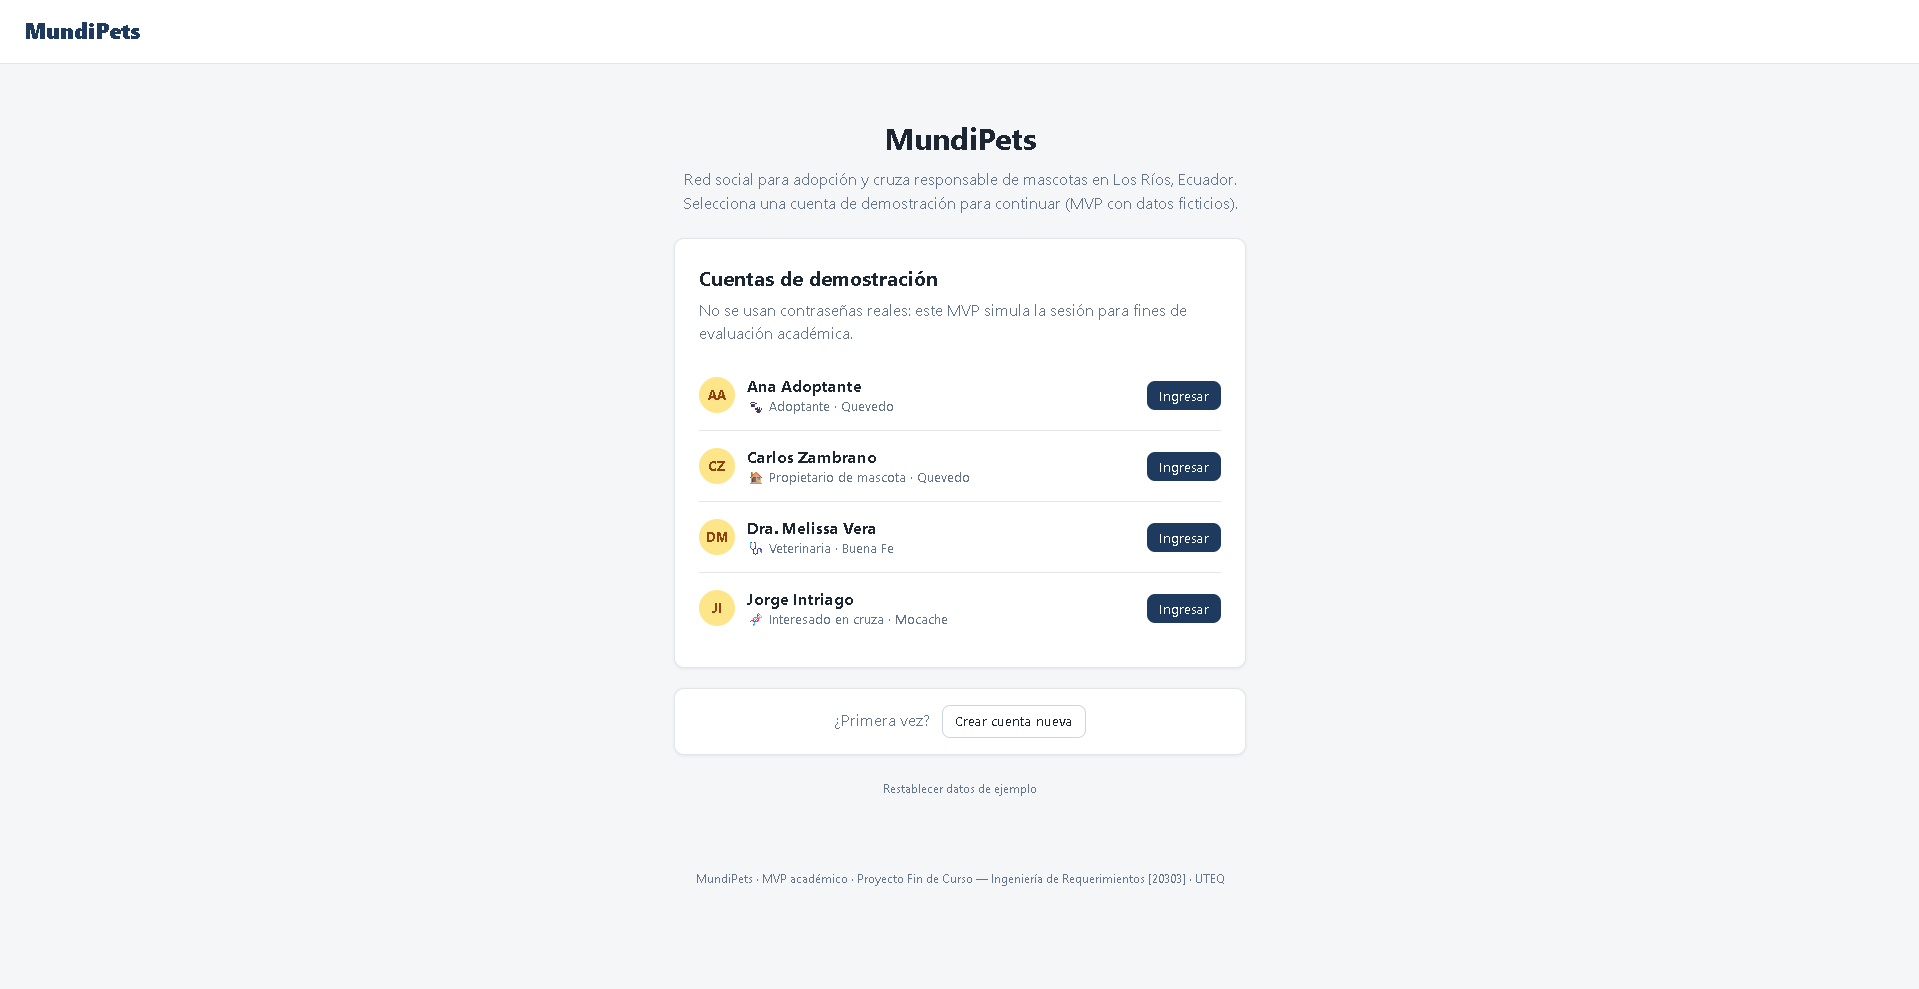
\includegraphics[width=0.92\textwidth]{figuras/MVP-01_InicioSesion_MundiPets.png}
		\caption{Pantalla de inicio de sesión del MVP (\texttt{index.html}). Se
			presentan las cuatro cuentas de demostración correspondientes a los roles
			del sistema --- Ana Adoptante, Carlos Zambrano (propietario), Dra. Melissa
			Vera (veterinaria) y Jorge Intriago (interesado en cruza) --- junto con la
			declaración explícita de que no se emplean contraseñas reales, que
			materializa la forma simulada de RF-12, y el enlace de restablecimiento
			de los datos de ejemplo.}
		\label{fig:mvp-login}
	\end{figure}
	
	\begin{figure}[H]
		\centering
		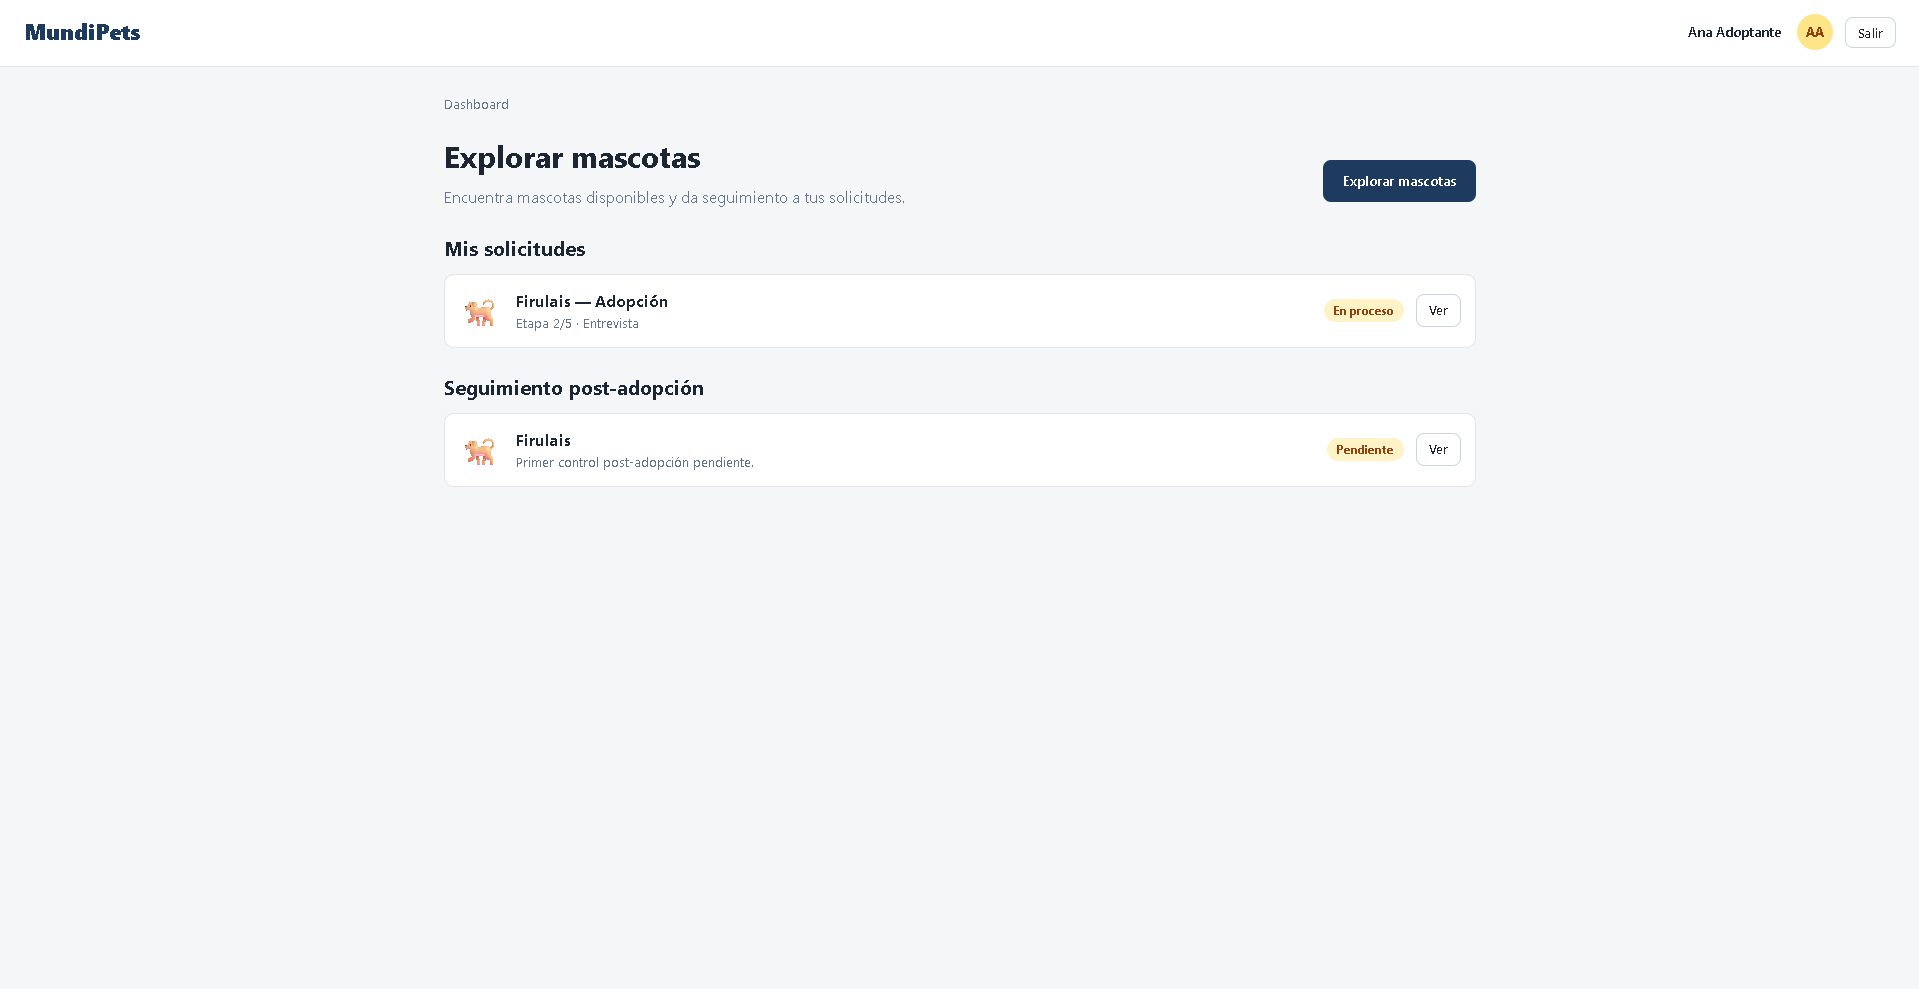
\includegraphics[width=0.92\textwidth]{figuras/MVP-02_PanelAdoptante_MundiPets.png}
		\caption{Panel de inicio diferenciado por rol (\texttt{dashboard.html}) para
			la cuenta de Ana Adoptante. La vista lista las solicitudes activas con su
			etapa vigente (\enquote{Etapa 2/5 --- Entrevista}) y los seguimientos
			post-adopción pendientes, evidenciando el acceso basado en roles de RD-02
			y los requisitos RF-18 y RF-22.}
		\label{fig:mvp-dashboard}
	\end{figure}
	
	\begin{figure}[H]
		\centering
		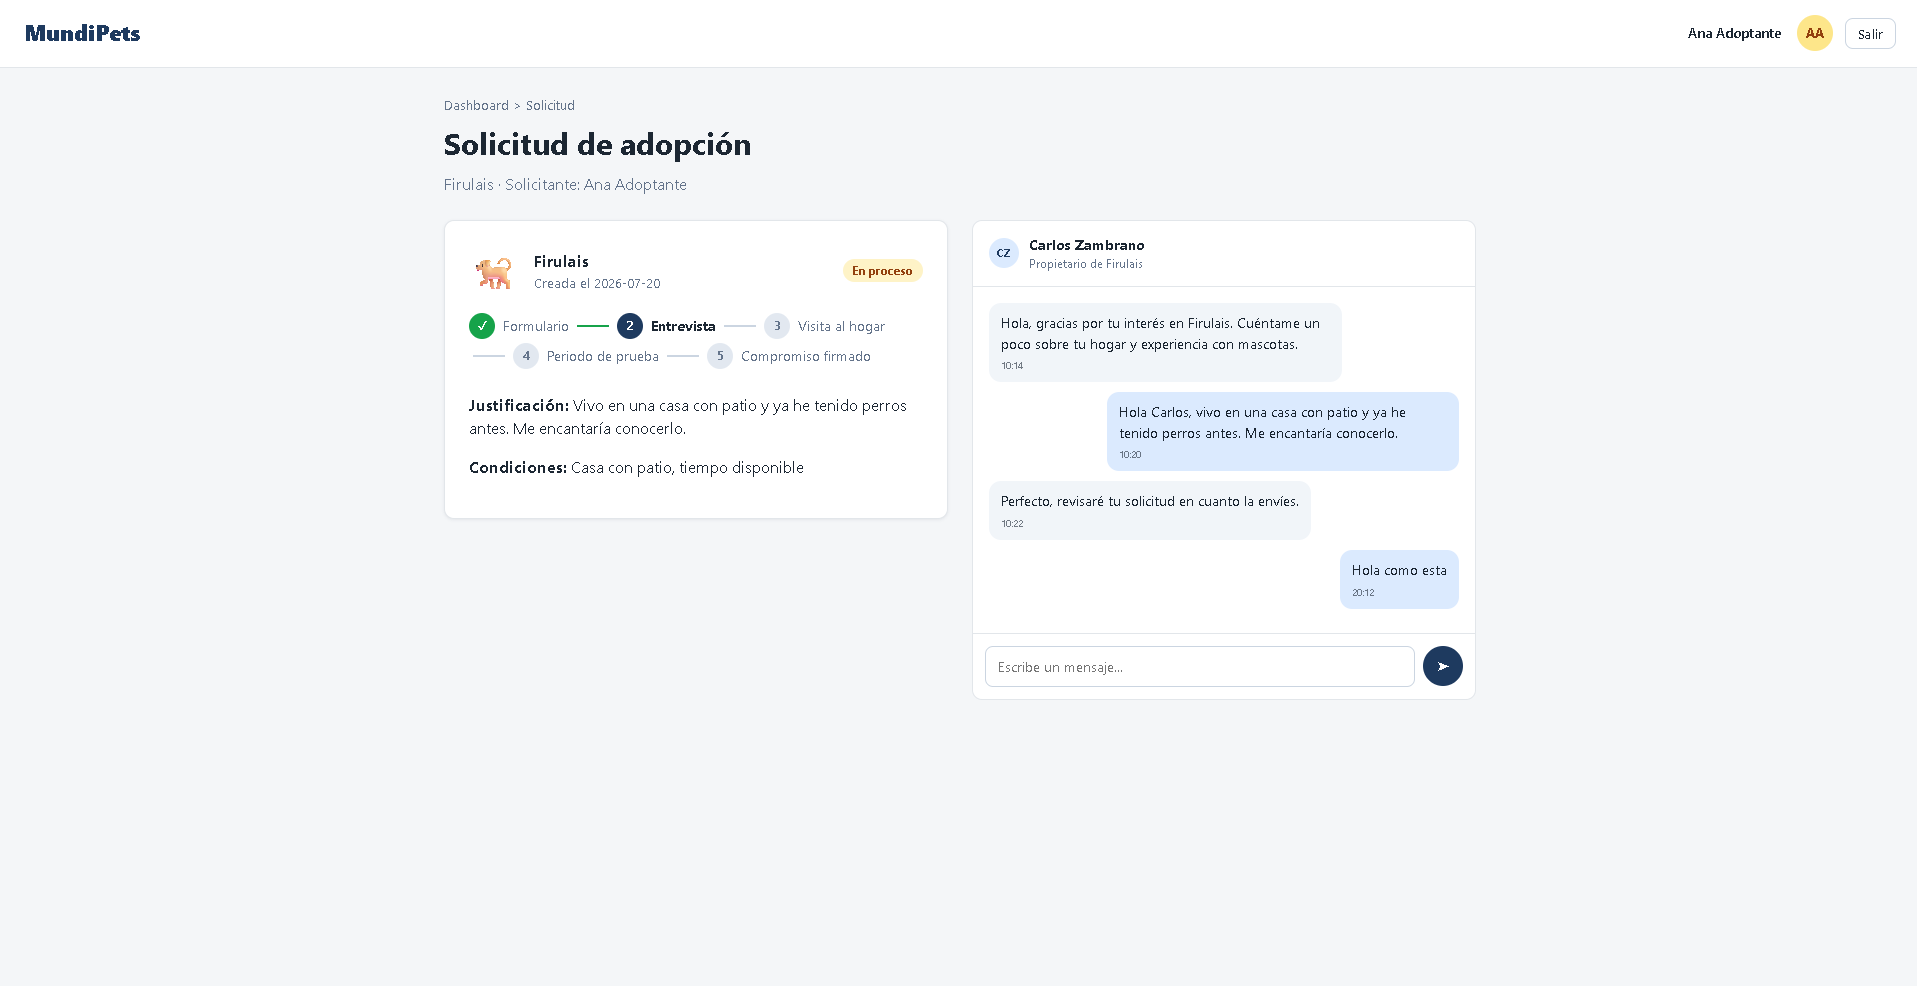
\includegraphics[width=0.92\textwidth]{figuras/MVP-03_SolicitudAdopcion_MundiPets.png}
		\caption{Detalle de una solicitud de adopción (\texttt{request.html}) con el
			indicador de las cinco etapas del proceso (formulario, entrevista, visita
			al hogar, periodo de prueba y compromiso firmado) y el panel de mensajería
			asociado a la solicitud, que implementan RF-05, RF-07 y RF-18.}
		\label{fig:mvp-solicitud}
	\end{figure}
	
	\begin{figure}[H]
		\centering
		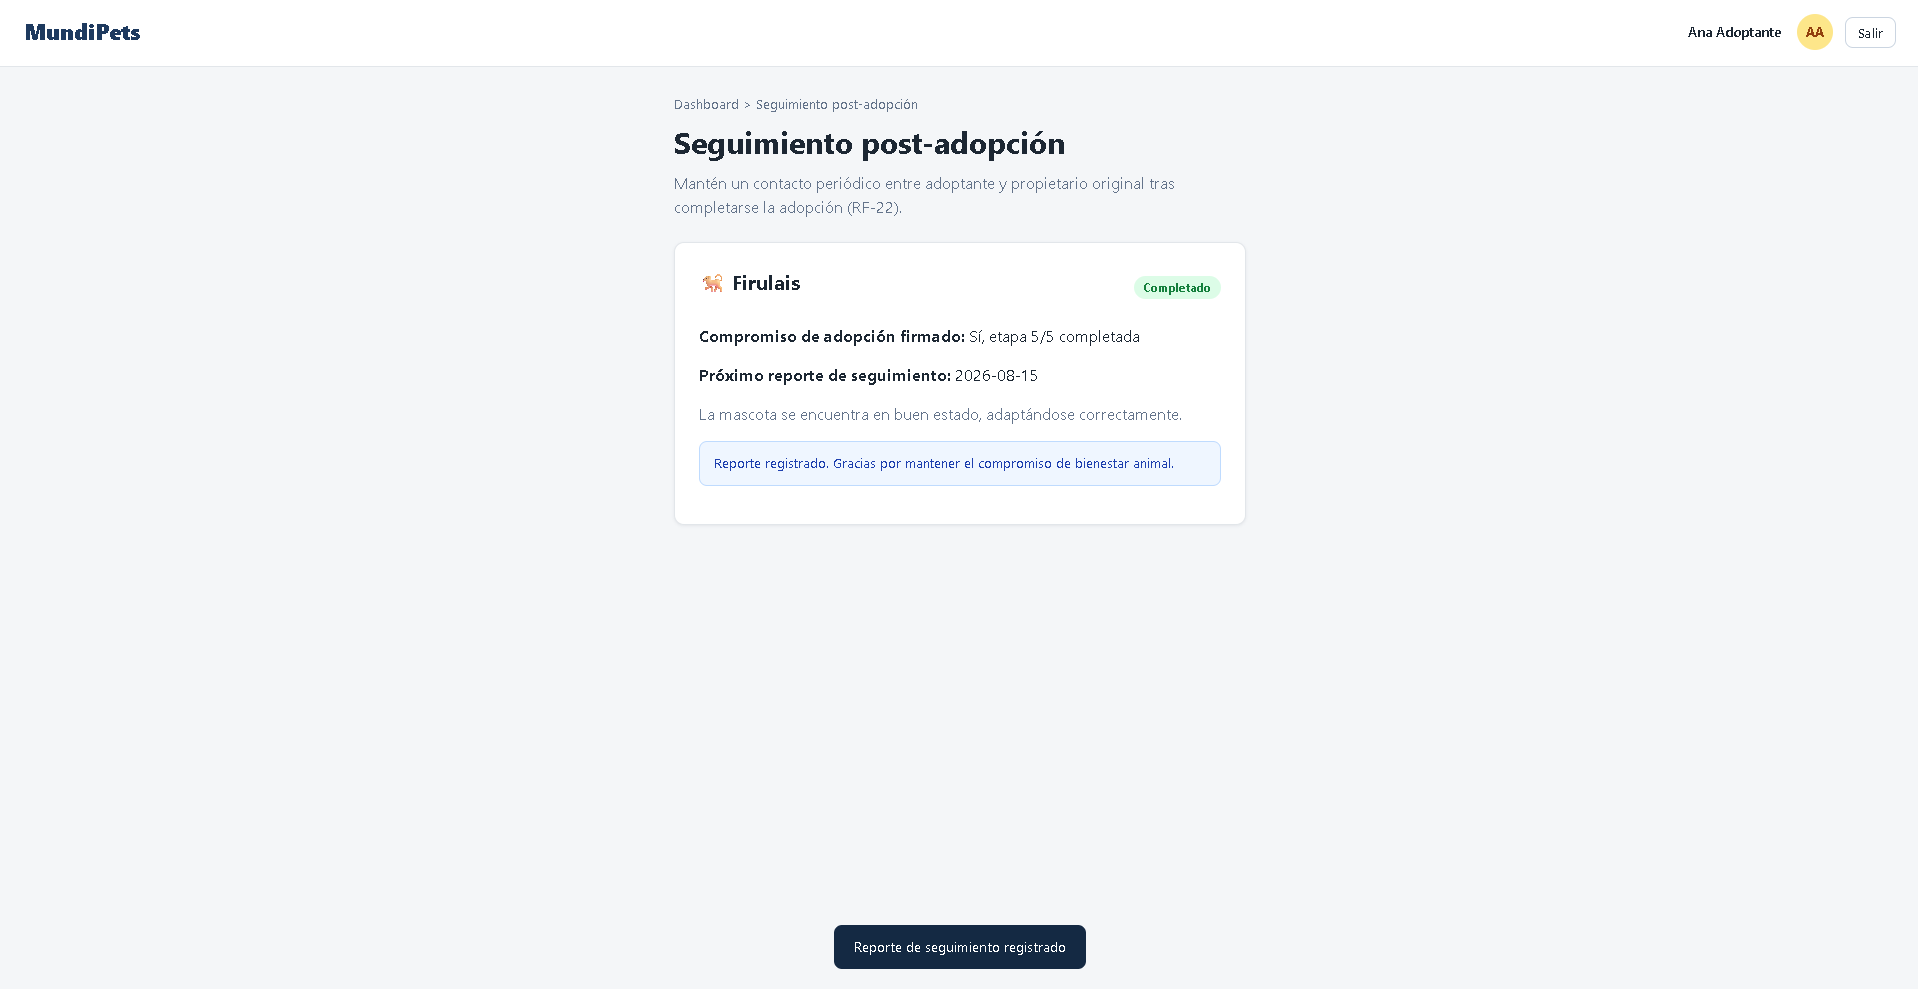
\includegraphics[width=0.92\textwidth]{figuras/MVP-04_SeguimientoPostAdopcion_MundiPets.png}
		\caption{Registro de seguimiento post-adopción (\texttt{post-adoption.html})
			generado automáticamente al completarse la quinta etapa de la solicitud.
			La vista muestra el compromiso firmado, la fecha del próximo reporte y el
			estado de la mascota adoptada, correspondientes a RF-22.}
		\label{fig:mvp-postadopcion}
	\end{figure}
	
	El video de recorrido funcional, de duración menor o igual a tres minutos,
	se encuentra en \texttt{05\_MVP/video\_demo.mp4}, y el enlace al repositorio
	público del MVP, junto con el commit exacto evaluado, se declara en
	\texttt{05\_MVP/README.md} y en el Apéndice~\ref{ap:repositorio}.
	
	% ############################################################
	%            SECCION 7 -- COMPONENTE EMPIRICO
	% ############################################################
	\section{Componente empírico del proyecto}
	\label{sec:empirico}
	
	\subsection{Enfoque seleccionado y justificación}
	\label{sec:enfoque}
	
	El equipo optó por el \textbf{Enfoque 2 --- Detectar automáticamente
		ambigüedad y malos olores en los requisitos}, descartando el Enfoque 1
	(comparación de la calidad de los RF frente a un LLM) y el Enfoque 3
	(validación de requisitos de explicabilidad del componente de IA).
	
	\textbf{Justificación en función del sistema.} MundiPets cuenta, desde la
	Entrega 2 (1B), con un corpus consolidado de especificación (17 RF, 8 RNF y
	5 restricciones de diseño), que constituye el insumo directo sobre el cual
	puede ejecutarse un detector de ambigüedad sin depender de instrumentos
	adicionales de recolección con usuarios externos al proyecto.
	
	\textbf{Justificación en función de los datos disponibles.} Como parte de la
	revisión y refinamiento del SRS parcial, el equipo ya efectuó un primer
	ejercicio de identificación manual de defectos de redacción sobre RF-01 a
	RF-17 y RNF-01 a RNF-08, detectando patrones de ambigüedad, terminología
	imprecisa y requisitos no verificables consistentes con los \emph{malos
		olores} descritos por Ferrari \emph{et al.} \cite{ferrari2016}. Este
	antecedente ofrece una base real sobre la cual diseñar y calibrar el
	detector automático, en lugar de partir desde cero.
	
	\textbf{Justificación en función del tiempo.} Independientemente del tiempo
	total disponible en el cronograma de la asignatura, el costo temporal de
	cada enfoque no depende solo de la duración del periodo, sino de la
	\emph{naturaleza de su ruta crítica}. Los Enfoques 1 y 3 dependen de
	reclutar y coordinar agendas con personas ajenas al equipo, lo cual introduce
	una latencia que no se reduce aunque se disponga de más semanas: el
	Enfoque 1 requiere entre tres y cinco personas evaluadoras externas
	dispuestas a calificar a ciegas dos conjuntos de al menos 50 RF cada uno, y
	el Enfoque 3 requiere doce participantes externos distribuidos en dos rondas
	de validación moderada, con la consiguiente necesidad de encontrar,
	convocar y agendar a cada uno. En ambos casos, el tiempo de ejecución queda
	sujeto a la disponibilidad de terceros, un factor fuera del control directo
	del equipo. El Enfoque 2, en cambio, mantiene su ruta crítica dentro del
	equipo: solo requiere tres personas expertas ya identificadas y la
	construcción de un detector automático (un script propio o una herramienta
	existente), ambas tareas ejecutables sin depender de la disponibilidad de
	terceros. Por esta razón, el Enfoque 2 ofrece el menor riesgo de cronograma
	de los tres, con independencia de cuántas semanas se le asignen.
	
	La decisión fue adoptada internamente por el equipo.
	
	\subsection{Preguntas de investigación en formato PICOC}
	\label{sec:rq}
	
	\begin{table}[H]
		\centering
		\caption{Preguntas de investigación estructuradas según el marco PICOC.}
		\label{tab:picoc}
		\small
		\begin{tabularx}{\textwidth}{@{}p{2.6cm} X@{}}
			\toprule
			\textbf{Elemento PICOC} & \textbf{Descripción} \\
			\midrule
			Población & Conjunto de requisitos funcionales (RF), no funcionales
			(RNF) y restricciones de diseño (RD) especificados para el sistema
			MundiPets, redactados según la plantilla de ocho atributos exigida
			por la asignatura y vigentes al momento de la ejecución del
			experimento. \\
			Intervención & Clasificación automática de cada requisito como
			\emph{ambiguo} o \emph{no ambiguo} mediante un detector basado en
			reglas, que identifica cuantificadores vagos, conjunciones
			múltiples que ocultan más de un requisito, voz pasiva y ausencia
			de criterio de verificación explícito. \\
			Comparación & Clasificación manual e independiente del mismo
			conjunto de requisitos, realizada por tres personas expertas en
			Ingeniería de Requisitos, sin conocimiento previo de la salida del
			detector (evaluación a ciegas). \\
			Resultado & Precisión, exhaustividad (\emph{recall}) y medida
			F1 del detector automático tomando como referencia el consenso
			experto; acuerdo inter-evaluador mediante $\kappa$ de Cohen entre
			pares de expertos y $\kappa$ de Fleiss para el conjunto de los
			tres. \\
			Contexto & Proyecto académico de la asignatura de Ingeniería de
			Requerimientos [20303] (UTEQ, 2026-2027 PPA), aplicado al sistema
			real MundiPets, con especificación redactada en español. \\
			\midrule
			RQ1 & ¿Con qué precisión, exhaustividad y medida F1 replica un
			detector automático basado en reglas el juicio consensuado de
			personas expertas al clasificar como ambiguos los requisitos
			especificados para MundiPets? \\
			RQ2 & ¿Qué patrones de desacuerdo predominan entre el detector
			automático y el juicio experto, y qué explican sobre las
			limitaciones de un enfoque basado en reglas frente al juicio
			humano en la identificación de ambigüedad? \\
			\bottomrule
		\end{tabularx}
	\end{table}
	
	\subsection{Hipótesis o proposiciones del estudio}
	\label{sec:hipotesis}
	
	Al tratarse del Enfoque 2, el diseño corresponde a un cuasi-experimento y
	requiere hipótesis nula y alternativa, no proposiciones de estudio de caso.
	
	\textbf{H\textsubscript{0} (hipótesis nula):} la clasificación producida
	por el detector automático de ambigüedad no guarda asociación con la
	clasificación de consenso de las personas expertas; el acuerdo observado
	entre ambas ($\kappa$ de Cohen) no es significativamente distinto del
	acuerdo esperado por azar ($\kappa = 0$).
	
	\textbf{H\textsubscript{1} (hipótesis alternativa):} la clasificación
	producida por el detector automático de ambigüedad guarda asociación
	significativa con la clasificación de consenso de las personas expertas;
	el acuerdo observado entre ambas es significativamente mayor que el
	esperado por azar ($\kappa > 0$).
	
	Esta hipótesis se contrasta mediante la prueba de significancia del
	$\kappa$ de Cohen descrita en la Sección \ref{sec:plan-analisis}. La
	pregunta RQ2, al ser de carácter exploratorio sobre los patrones de
	desacuerdo, no se somete a prueba de hipótesis: se responde mediante
	análisis cualitativo de los casos en los que el detector y el consenso
	experto difieren, siguiendo el sexto paso descrito para el Enfoque 2 en la
	guía de la asignatura.
	
	\subsection{Variables independientes, dependientes y de control}
	\label{sec:variables}
	
	\textbf{Variable independiente.} El método de clasificación aplicado a
	cada requisito, con dos niveles: (a) detector automático basado en reglas
	y (b) consenso de las tres personas expertas.
	
	\textbf{Variable dependiente.} La clasificación resultante de cada
	requisito como \emph{ambiguo} o \emph{no ambiguo} (variable categórica
	binaria), a partir de la cual se calculan las métricas de acuerdo
	declaradas en la Sección \ref{sec:plan-analisis} (precisión, exhaustividad,
	medida F1 y $\kappa$).
	
	\textbf{Variables de control.}
	\begin{itemize}[leftmargin=*]
		\item \textbf{Tipo de requisito} (RF, RNF o RD), para verificar que el
		desempeño del detector no varíe sistemáticamente según el tipo de
		artefacto evaluado.
		\item \textbf{Configuración fija del detector}: el conjunto de reglas
		(cuantificadores vagos, conjunciones múltiples, voz pasiva, ausencia de
		criterio de verificación) permanece invariable durante toda la
		ejecución del experimento; ninguna regla se ajusta después de observar
		resultados parciales.
		\item \textbf{Orden de presentación} de los requisitos a las personas
		expertas, aleatorizado de forma independiente para cada evaluador, con
		el fin de controlar efectos de fatiga o de orden.
		\item \textbf{Cegamiento del juicio experto}: ninguna persona
		evaluadora tiene acceso a la salida del detector ni a la clasificación
		de las demás personas evaluadoras antes de completar la propia.
	\end{itemize}
	
	\subsection{Participantes y reclutamiento}
	\label{sec:participantes}
	
	El estudio involucra dos grupos con roles distintos: las personas expertas
	que ejecutan la clasificación de referencia, y el equipo de MundiPets, que
	construye y aplica el detector automático sin participar en la
	clasificación experta, para preservar la independencia del juicio.
	
	\textbf{Personas expertas.} El panel está compuesto por tres Ingenieros de
	Software graduados de la Universidad Técnica Estatal de Quevedo (UTEQ) (dos
	mujeres y un hombre), ya contactados y confirmados para participar en el
	estudio.
	
	\textbf{Criterios de inclusión:} (a) título profesional de tercer nivel en
	Ingeniería de Software o carrera afín; (b) formación o experiencia
	demostrable en especificación y análisis de requisitos de software; (c)
	disponibilidad para completar la clasificación dentro del cronograma del
	estudio.
	
	\textbf{Criterios de exclusión:} (a) pertenecer al equipo de desarrollo de
	MundiPets; (b) haber participado en la redacción de los RF, RNF o RD que
	conforman la población del estudio (Sección \ref{sec:rq}).
	
	\textbf{Proceso de consentimiento informado.} Cada persona evaluadora firma
	un consentimiento informado específico para este rol, redactado en
	cumplimiento de la Ley Orgánica de Protección de Datos Personales del
	Ecuador \cite{lopdp2021}, que autoriza expresamente su participación como
	evaluadora experta y el uso de la clasificación producida --de forma
	anonimizada-- en publicaciones científicas revisadas por pares. La
	plantilla se detalla en la Sección \ref{sec:instrumentos}.
	
	\subsection{Instrumentos}
	\label{sec:instrumentos}
	
	Los instrumentos del Enfoque 2 son dos:
	
	\begin{enumerate}[leftmargin=*]
		\item \textbf{Rúbrica de clasificación experta}
		(\texttt{rubrica\_clasificacion\_experta.xlsx}): libro con hoja de
		instrucciones, hoja de criterios de referencia para identificar
		ambigüedad, y hoja de evaluación en la que cada persona evaluadora
		registra, para cada requisito, su identificador, el texto completo,
		la clasificación (\emph{ambiguo} / \emph{no ambiguo}), el tipo de
		mal olor detectado y una justificación breve. Los requisitos se
		presentan sin indicar su tipo (RF, RNF o RD) y en orden aleatorizado,
		para reducir sesgos de expectativa. Una hoja adicional, de uso
		exclusivo del equipo, conserva la clave que vincula cada identificador
		anónimo con el requisito real y la salida del detector.
		\item \textbf{Plantilla de consentimiento para evaluadores expertos}
		(\texttt{consentimiento\_evaluador\_experto.docx}): adapta el formato
		de consentimiento ya utilizado en la Entrega 1B para entrevistas,
		ajustado al rol de evaluador experto e incorporando la autorización
		explícita para el uso de datos anonimizados en publicaciones
		revisadas por pares, conforme a la LOPDP \cite{lopdp2021}.
	\end{enumerate}
	
	\subsection{Plan de análisis estadístico}
	\label{sec:plan-analisis}
	
	\textbf{Análisis principal (RQ1, H\textsubscript{0}/H\textsubscript{1}).}
	Se calculan precisión, exhaustividad y medida F1 del detector automático
	tomando como referencia el consenso experto (Sección \ref{sec:hipotesis}).
	La hipótesis se contrasta mediante una prueba de significancia del $\kappa$
	de Cohen (estadístico $z = \kappa / SE_{\kappa}$, contra la distribución
	normal estándar), mientras que la magnitud del acuerdo se interpreta como
	el tamaño del efecto, usando la escala de Landis y Koch: 0,00--0,20 leve;
	0,21--0,40 aceptable; 0,41--0,60 moderado; 0,61--0,80 sustancial;
	0,81--1,00 casi perfecto.
	
	\textbf{Acuerdo inter-evaluador.} $\kappa$ de Cohen \cite{cohen1960} para
	cada par de las tres personas expertas, y $\kappa$ de Fleiss
	\cite{fleiss1971} para el conjunto de las tres, interpretados con la misma
	escala de Landis y Koch. Un acuerdo experto bajo relativizaría cualquier
	conclusión sobre el desempeño del detector, ya que el propio consenso de
	referencia quedaría en duda.
	
	\textbf{Prueba de normalidad (Shapiro-Wilk).} Se aplica sobre la variable
	continua \emph{nivel de confianza} (escala 1--5) registrada en la rúbrica
	de evaluación (Sección \ref{sec:instrumentos}), como paso previo al
	análisis exploratorio secundario descrito a continuación.
	
	\textbf{Análisis secundario (RQ2, exploratorio).} Para caracterizar los
	casos de desacuerdo entre el detector y el consenso experto, se compara el
	nivel de confianza reportado por las personas expertas entre los
	requisitos donde el detector coincide con el consenso y aquellos donde
	difiere. Si Shapiro-Wilk no rechaza normalidad, se usa la prueba t de
	Student para muestras independientes y el tamaño del efecto se reporta
	como $d$ de Cohen; en caso contrario, se usa la prueba U de Mann-Whitney y
	el tamaño del efecto como $\delta$ de Cliff. Este análisis es exploratorio
	y se complementa con la nota cualitativa de desacuerdos exigida por el
	sexto paso del Enfoque 2 en la guía de la asignatura.
	
	\textbf{Corrección por comparaciones múltiples.} Si además se reportan
	métricas de acuerdo desagregadas por tipo de requisito (RF, RNF, RD) como
	análisis exploratorio adicional, los valores $p$ resultantes de esas tres
	comparaciones relacionadas se ajustan mediante el procedimiento de
	Benjamini-Hochberg (control de la tasa de falsos descubrimientos).
	
	\textbf{Cálculo de potencia estadística.} Conforme a Molléri \emph{et al.}
	\cite{molleri2020} y Wohlin \emph{et al.} \cite{wohlin2012}, se fija
	$\alpha = 0{,}05$ y $1 - \beta = 0{,}80$. Dado que el tamaño de la
	población está acotado por el corpus real de especificación disponible
	(Sección \ref{sec:enfoque}) y no por una meta de reclutamiento ampliable,
	el cálculo de potencia se reporta en sentido inverso: en lugar de fijar un
	$N$ objetivo, se determina la sensibilidad mínima (el valor mínimo de
	$\kappa$ detectable) que el diseño puede identificar con ese $\alpha$ y
	esa potencia, dado el $N$ realmente disponible al momento de la ejecución.
	Este cálculo se documentará con el valor real de $N$ y se versionará junto
	con el resto del análisis.
	
	\textbf{Reproducibilidad.} Todos los cálculos anteriores se ejecutan
	mediante scripts versionados en \texttt{06\_Experimento/scripts\_analisis/}
	(Python, con \texttt{SciPy}/\texttt{statsmodels} o R); ninguna cifra o
	tabla de esta sección se produce de forma manual, conforme a la regla de
	la guía de la asignatura.
	
	\subsection{Registro previo del protocolo en el OSF}
	\label{sec:osf}
	
	El protocolo del Enfoque 2 se registró en el Open Science Framework
	\cite{nosek2018}, mediante la plantilla \emph{OSF Preregistration}, el
	\textbf{27 de julio de 2026 a las 10:49:41 a.\,m.} (hora de Ecuador), antes
	de distribuir la rúbrica de clasificación al panel experto y antes de
	ejecutar el detector automático sobre el corpus de requisitos. El registro
	puede consultarse en:
	\url{https://osf.io/khyf2/overview}.
	El registro fue \textbf{aceptado} tras la moderación estándar de OSF
	posterior al envío. La marca de tiempo corresponde al momento del envío, en
	el que el contenido del registro queda congelado, con independencia de la
	fecha de aprobación.
	
	\subsection{Amenazas a la validez previstas}
	\label{sec:amenazas}
	
	\textbf{Validez interna.}
	\begin{itemize}[leftmargin=*]
		\item \emph{Sesgo de diseño del detector.} El equipo que construye el
		detector ya conoce, por la revisión manual previa realizada durante
		el refinamiento del SRS parcial (Sección \ref{sec:enfoque}), algunos
		de los defectos presentes en RF-01 a RF-17, lo que podría calibrar
		las reglas hacia esos casos conocidos e inflar artificialmente la
		precisión. \textbf{Mitigación:}
		las reglas del detector (Sección \ref{sec:enfoque}) se fijan y
		documentan antes de recibir la clasificación de los tres expertos
		sobre el conjunto completo, y se aplican sin modificación posterior
		(Sección \ref{sec:variables}). \textbf{Limitación reconocida:} el
		sesgo no se elimina por completo, porque el conocimiento previo del
		equipo sobre una parte del corpus es inevitable; se atenúa
		parcialmente al incluir en la población los RF-18 a RF-25, que no
		formaron parte de esa revisión previa.
		\item \emph{Efecto de orden o fatiga en la evaluación experta.}
		Evaluar un conjunto largo de requisitos de forma consecutiva puede
		degradar el juicio hacia el final del ejercicio. \textbf{Mitigación:}
		orden de presentación aleatorizado de forma independiente para cada
		evaluador (Sección \ref{sec:variables}). \textbf{Limitación
			reconocida:} la aleatorización distribuye el efecto pero no lo
		elimina; no se mide directamente si la fatiga afectó casos
		específicos.
	\end{itemize}
	
	\textbf{Validez externa.}
	\begin{itemize}[leftmargin=*]
		\item \emph{Corpus de un solo sistema y dominio.} Los requisitos
		provienen únicamente de MundiPets, redactados en español por un solo
		equipo estudiantil en el dominio veterinario/adopción de mascotas.
		\textbf{Mitigación:} el contexto queda documentado explícitamente en
		el marco PICOC (Sección \ref{sec:rq}) para que cualquier lector pueda
		evaluar la transferibilidad. \textbf{Limitación reconocida:} no puede
		afirmarse que el desempeño del detector generalice a otros dominios,
		idiomas o equipos con distinto nivel de experiencia; el estudio se
		declara como un caso único, no como una validación general del
		detector.
		\item \emph{Homogeneidad del panel experto.} Las tres personas
		evaluadoras son Ingenieras e Ingeniero de Software graduados de la
		misma universidad (UTEQ). \textbf{Mitigación:} el perfil exacto del
		panel se documenta en la Sección \ref{sec:participantes}.
		\textbf{Limitación reconocida:} no se garantiza representatividad de
		la diversidad de juicio experto que existiría con un panel de otras
		instituciones o con mayor trayectoria profesional.
	\end{itemize}
	
	\textbf{Validez de constructo.}
	\begin{itemize}[leftmargin=*]
		\item \emph{Binarización de un fenómeno gradual.} La ambigüedad
		rara vez es todo-o-nada; reducirla a \emph{ambiguo}/\emph{no ambiguo}
		simplifica un constructo más complejo. \textbf{Mitigación:} la
		rúbrica captura matices adicionales mediante el campo \emph{tipo de
			mal olor detectado} y el \emph{nivel de confianza} (Sección
		\ref{sec:instrumentos}). \textbf{Limitación reconocida:} la variable
		principal de análisis sigue siendo binaria; se acepta esta
		simplificación como necesaria para el análisis cuantitativo dentro
		del tiempo disponible.
		\item \emph{Alcance limitado de un detector basado en reglas.} El
		detector identifica ambigüedad léxica y sintáctica (cuantificadores
		vagos, voz pasiva, conjunciones múltiples), pero no ambigüedad
		semántica de dominio que solo una persona con conocimiento
		veterinario puede reconocer. \textbf{Mitigación:} el alcance de las
		reglas se documenta explícitamente y no se presenta el detector como
		un sustituto general del juicio experto. \textbf{Limitación
			reconocida:} la comparación mide específicamente cuánta ambigüedad
		\emph{detectable por reglas léxicas} coincide con el juicio experto
		global, no toda forma posible de ambigüedad.
	\end{itemize}
	
	\textbf{Validez de conclusión.}
	\begin{itemize}[leftmargin=*]
		\item \emph{Tamaño de muestra reducido.} La población disponible
		(Sección \ref{sec:enfoque}) es menor al mínimo de 50 requisitos
		sugerido por la guía de la asignatura para este enfoque, lo que
		reduce la potencia para detectar valores pequeños de $\kappa$ como
		significativamente distintos de cero. \textbf{Mitigación:} el plan
		de análisis (Sección \ref{sec:plan-analisis}) reporta explícitamente
		la sensibilidad mínima detectable dado el $N$ real, en vez de ocultar
		la limitación. \textbf{Limitación reconocida:} con un $N$ reducido,
		el estudio puede no tener potencia suficiente para detectar niveles
		de acuerdo moderados-bajos como estadísticamente significativos; los
		resultados de la Entrega 4 deberán interpretarse con este límite en
		mente.
		\item \emph{Panel experto mínimo.} Solo tres personas conforman el
		consenso de referencia, el mínimo aceptado por la guía; con un panel
		tan pequeño, la opinión de una sola persona pesa proporcionalmente
		más sobre el consenso. \textbf{Mitigación:} se calcula
		explícitamente el acuerdo inter-evaluador mediante $\kappa$ de Fleiss
		antes de aceptar el consenso como válido. \textbf{Limitación
			reconocida:} un panel de tres es más vulnerable a la idiosincrasia
		individual que el panel de cinco recomendado por la guía, al que no
		se llega por restricciones de tiempo.
	\end{itemize}
	
	% ############################################################
	%                    SECCION 8 -- CONCLUSIONES
	% ############################################################
	
	% ############################################################
	%                    SECCION 8 -- CONCLUSIONES
	% ############################################################
	\section{Conclusiones}
	\label{sec:conclusiones}
	
	Esta entrega consolida la Especificación de Requisitos de Software de
	MundiPets como un documento completo, verificable y sustentado en evidencia
	de campo. El resultado principal es que la totalidad de los requisitos
	especificados --- 27 requisitos funcionales, 16 no funcionales y 9
	restricciones de diseño --- queda trazada hasta al menos una evidencia
	primaria del catálogo del Apéndice~B.1, y ninguna afirmación sustantiva del
	documento se apoya únicamente en la deliberación interna del equipo.
	
	\paragraph{Sobre la completitud de la especificación.}
	La segunda ronda de campo amplió el corpus de evidencias de 8 a 24 unidades,
	incorporando entrevistas adicionales, un cuestionario con 61 respuestas
	válidas y seis sesiones de validación \emph{walkthrough} con usuarios
	técnicos y no técnicos. La curva de saturación temática
	(Sección~\ref{sec:codificacion}) alcanza cero códigos nuevos en la evidencia
	EV-17, lo que indica que el corpus de elicitación llegó al punto de
	saturación antes de cerrar la ronda. Los ocho requisitos incorporados en esta
	entrega (RF-18 a RF-25) no surgieron de una revisión de escritorio sino de
	necesidades expresadas por participantes concretos, lo que explica que la
	especificación crezca sin que la saturación se vea contradicha: las
	entrevistas finales aportaron matices sobre categorías ya identificadas más
	que categorías nuevas.
	
	\paragraph{Sobre el marco legal y la explicabilidad.}
	El mapeo de la Ley Orgánica de Protección de Datos Personales del Ecuador
	\cite{lopdp2021} contra los requisitos (Sección~\ref{sec:legales}) mostró que
	el marco legal no es un anexo del diseño sino una fuente de requisitos por
	derecho propio: el Art.~20, sobre decisiones automatizadas, es la base
	directa de los tres requisitos de explicabilidad (RNF-13, RNF-14 y RNF-15),
	que de otro modo se habrían tratado como una preocupación de usabilidad. La
	decisión de tratar la explicabilidad como requisito no funcional medible,
	siguiendo a Chazette y Schneider \cite{chazette2020}, obligó a definir
	métricas concretas --- extensión máxima de la explicación, tiempo de
	generación y comprensión reportada --- en lugar de enunciados genéricos sobre
	transparencia.
	
	\paragraph{Sobre las limitaciones reconocidas.}
	El documento declara de forma expresa el alcance de sus decisiones de
	diseño, en lugar de presentarlas de manera implícita. La clasificación
	según el modelo de Kano se reporta como una aproximación de un solo
	factor, y no como una clasificación Kano completa, porque el cuestionario
	v2.0 midió importancia declarada pero no incluyó el par de preguntas
	funcional y disfuncional que el modelo exige (Sección~\ref{sec:kano}).
	Del mismo modo, tres requisitos funcionales de prioridad \emph{Must}
	(RF-18, RF-22 y RF-23) no cuentan con una pantalla de alta fidelidad
	propia, por diseño y no por omisión: sus interacciones se resuelven como
	transiciones de estado y avisos superpuestos sobre las pantallas ya
	construidas (Sección~\ref{sec:mockups}), decisión que queda trazada de
	forma explícita en el Apéndice~D. Declarar estos límites de alcance
	fortalece, en lugar de debilitar, la validez de las conclusiones del
	estudio.
	
	\paragraph{Sobre el componente empírico.}
	El protocolo del estudio de detección automática de ambigüedad quedó
	registrado en el Open Science Framework antes de iniciar la recolección de
	datos, lo que fija la marca temporal del diseño con independencia de los
	resultados obtenidos. Esta decisión metodológica es la que permite, en el
	cierre de la Entrega 4, reportar los hallazgos sin sospecha de ajuste
	posterior de las hipótesis. El plan de análisis estadístico se ejecuta
	sobre los datos recolectados en las tres rondas de campo, y el paquete de
	datos anonimizado se consolida para su depósito con identificador
	persistente, siguiendo los principios FAIR \cite{wilkinson2016} y las
	prácticas de citación de software \cite{smith2016}.
	
	% ############################################################
	%                        REFERENCIAS
	% ############################################################
	\newpage
	\printbibliography[title={Referencias}]
	\addcontentsline{toc}{section}{Referencias}
	
	% ############################################################
	%                        APENDICES
	% ############################################################
	\newpage
	\appendix
	
	% --------------------------------------------------------
	\section*{Apéndice A --- Plan del proyecto de IR}
	\addcontentsline{toc}{section}{Apéndice A --- Plan del proyecto de IR}
	\label{ap:plan}
	
	\textbf{Roles del equipo (vigentes para la Entrega 4, 2B):}
	
	\begin{table}[H]
		\caption{Roles asignados al equipo del proyecto MundiPets.}
		\centering
		\begin{tabularx}{\linewidth}{|X|X|}
			\hline
			\textbf{Integrante} & \textbf{Rol} \\
			\hline
			Fuertes Arraes Edson Daniel & Analista líder -- coordina el equipo, valida con el cliente, redacta los requisitos funcionales e historias de usuario, gestiona el repositorio. \\
			\hline
			Gutiérrez Ortega Génesis Adriana & Verificador -- controla la calidad de los requisitos no funcionales, la explicabilidad, el marco legal y las evidencias de campo. \\
			\hline
			Mendoza Párraga Andy Johel & Modelador -- construye los ocho diagramas UML exigidos y los mockups de alta fidelidad. \\
			\hline
			Morales Sánchez Gary Alejandro & Documentador -- estructura el ERS/SRS según IEEE 29148, contexto, modelado organizacional y trazabilidad. \\
			\hline
			Nieves Sánchez Jimmy Samuel & Verificador -- responsable del componente empírico, el MVP y el paquete de publicación. \\
			\hline
		\end{tabularx}
	\end{table}
	
	\textbf{Cronograma del proyecto (actualizado a la Entrega 4, 2B):}
	
	\begin{table}[H]
		\caption{Cronograma de la Ingeniería de Requisitos -- MundiPets (Semestre 2026-2027 PPA).}
		\centering
		
		\begin{tabularx}{\linewidth}{|C{2.5cm}|X|C{2.8cm}|}
			\hline
			\textbf{Semana / Fecha} & \textbf{Actividad} & \textbf{Estado} \\
			\hline
			Semanas 1--3 (04--24 may.) & Selección del sistema real (MundiPets), planificación de la Ingeniería de Requisitos y definición de roles del equipo. & Completado \\
			\hline
			\textbf{Semana 4 (25--31 may.)} & \textbf{Primer avance:} Planificación + Elicitación inicial (Entrega 1A). Ejecución de entrevistas estructuradas a stakeholders (17--29 may.). & Completado \\
			\hline
			Semanas 5--8 (01--28 jun.) & Consolidación de requisitos crudos, análisis y clasificación (RF/RNF/restricciones), modelado UML inicial (casos de uso y clases conceptual). & Completado \\
			\hline
			\textbf{Semana 9 (29 jun.--05 jul.)} & \textbf{Segundo avance:} ERS/SRS parcial -- requisitos formalizados (plantilla de 8 atributos), RNF cuantificados, modelado UML e interfaces, priorización MoSCoW y trazabilidad parcial (Entrega 2/1B). & Completado \\
			\hline
			Semanas 10--11 (06--19 jul.) & Segunda ronda de elicitación: entrevistas y sesiones de walkthrough adicionales, ampliación del cuestionario (v2.0) para cubrir Kano, codificación temática de las transcripciones y curva de saturación. & Completado \\
			\hline
			Semana 12 (20--26 jul.) & Redacción de los RF-18 a RF-25 y RNF-09 a RNF-15 a partir de la codificación temática, mapeo legal LOPDP, construcción del diagrama de Razón Estratégica (SR) y refinamiento del diagrama de clases. & Completado \\
			\hline
			\textbf{Semana 13 (27 jul.--02 ago.)} & \textbf{Tercer avance:} ERS Completo con Validación y Trazabilidad -- documento de especificación de requisitos completo, validado y con trazabilidad total evidencia--requisito--caso de uso, priorización Kano/WSJF, MVP y protocolo del componente empírico registrado en el OSF. & Completado \\
			\hline
			Semanas 14--16 (03--23 ago.) & Ejecución del componente empírico, desarrollo del MVP (ampliado a 26 de 27 RF cubiertos), segunda ronda de \emph{walkthrough} con PROP-12 y VET-07 (EV-23, EV-24), revisión integral del documento y ajustes finales según observaciones del docente. & Completado \\
			\hline
			\textbf{Semana 17 (24--30 ago.)} & \textbf{Cuarto avance:} Proyecto Integrador Final -- corrección de calidad de los 25 RF vigentes conforme a ISO/IEC/IEEE 29148:2018, incorporación de RF-26 y RF-27 a partir de la nueva evidencia de campo, actualización de la matriz de trazabilidad extendida (61 filas, incluidos los 9 requisitos legales) y entrega y sustentación del documento ERS/SRS completo del Proyecto Fin de Curso. & Completado \\
			\hline
		\end{tabularx}
	\end{table}
	
	\textbf{Técnicas de elicitación seleccionadas:}
	
	Para esta entrega se mantiene la entrevista estructurada como técnica
	principal, complementada con sesiones de \emph{walkthrough} para la
	validación de los requisitos ya especificados. La segunda ronda de campo
	amplía el cuestionario aplicado en la 1B (versión 2.0) con las preguntas
	funcional y disfuncional del modelo de Kano para cada funcionalidad candidata,
	de modo que la priorización Kano de la Sección~\ref{sec:kano} quede
	respaldada por datos reales y no por criterio de escritorio. Esta técnica se
	complementa con la codificación temática de las transcripciones
	(Apéndice~B.8), que es el insumo directo para derivar los ocho requisitos
	funcionales nuevos (RF-18 a RF-25) exigidos por la Entrega 3 (2A). En la
	presente revisión (4.0) se ejecutaron dos sesiones adicionales que
	combinan entrevista y \emph{walkthrough} sobre el mismo participante,
	EV-23 (PROP-12, propietaria de mascota, usuaria no técnica) y EV-24
	(VET-07, veterinaria, usuaria técnica), con lo que la ronda de validación
	alcanza las 6 sesiones mínimas exigidas (3 técnicas y 3 no técnicas,
	Apéndice~B.7). Estas dos evidencias son el origen directo de RF-27 y
	RF-26, respectivamente.
	
	% --------------------------------------------------------
	\section*{Apéndice B --- Trabajo de campo y evidencias}
	\addcontentsline{toc}{section}{Apéndice B --- Trabajo de campo y evidencias}
	\label{ap:evidencias}
	
	\subsection*{B.1 Registro y catálogo de evidencias}
	
	La Tabla~\ref{tab:catalogo-evidencias} consolida las veinticuatro evidencias
	de campo recogidas por el equipo, indicando el tipo de instrumento
	aplicado, el participante o fuente, los requisitos derivados de cada una y
	si se cuenta con el consentimiento informado firmado correspondiente
	(Apéndice~B.6). Las dos últimas (EV-23 y EV-24), incorporadas en la
	revisión 4.0, combinan entrevista y sesión de validación
	\emph{walkthrough} sobre el mismo participante.
	
	\textbf{Codificación de participantes.} En cumplimiento de la restricción
	RD-09 y de la Ley Orgánica de Protección de Datos Personales del Ecuador
	\cite{lopdp2021}, ninguna persona participante se identifica por su nombre
	en este documento ni en los artefactos públicos del repositorio. Se emplean
	códigos de participante con el prefijo \texttt{PROP-XX} para propietarios de
	mascota, \texttt{VET-XX} para profesionales veterinarios y \texttt{OBS-XX}
	para establecimientos observados. La tabla de correspondencia entre código y
	persona real no se publica: permanece en la zona restringida
	(\texttt{02\_Evidencias/00\_Restringido/}) bajo custodia del equipo y del
	docente responsable. Una misma persona puede estar asociada a más de una
	evidencia; por ejemplo, quien participó en una entrevista y posteriormente
	en una sesión de validación conserva el mismo código.
	
	{\small
		\begin{longtable}{@{}>{\raggedright\arraybackslash}p{1.2cm} >{\raggedright\arraybackslash}p{3.1cm} >{\raggedright\arraybackslash}p{3.1cm} >{\raggedright\arraybackslash}p{6.0cm} >{\raggedright\arraybackslash}p{1.4cm}@{}}
			\caption{Registro y catálogo de evidencias del trabajo de campo.}
			\label{tab:catalogo-evidencias}\\
			\toprule
			\textbf{ID-EV} & \textbf{Tipo de evidencia} & \textbf{Fuente / participante} & \textbf{Requisitos derivados} & \textbf{Consent.} \\
			\midrule
			\endfirsthead
			\multicolumn{5}{@{}l}{\small\itshape (continuación)}\\
			\toprule
			\textbf{ID-EV} & \textbf{Tipo de evidencia} & \textbf{Fuente / participante} & \textbf{Requisitos derivados} & \textbf{Consent.} \\
			\midrule
			\endhead
			\bottomrule
			\endlastfoot
			EV-01 & Entrevista grabada, audio, video y consentimiento & PROP-01 (propietario de mascota) & RF-01, RF-03, RF-05, RF-07, RF-08, RF-12, RF-13 & Sí \\
			\addlinespace
			EV-02 & Entrevista grabada, audio, video y consentimiento & PROP-02 (propietaria de mascota) & RF-01, RF-02, RF-03, RF-05, RF-07, RF-08, RF-10, RF-11, RF-13, RF-14, RF-15 & Sí \\
			\addlinespace
			EV-03 & Entrevista grabada, audio, video y consentimiento & VET-01 (médica veterinaria) & RF-01, RF-02, RF-05, RF-06, RF-08, RF-09, RF-12, RF-14, RF-16, RF-17, RNF-01, RNF-05, RNF-06, RNF-07, RD-03, RD-04 & Sí \\
			\addlinespace
			EV-04 & Entrevista grabada, audio, video y consentimiento & VET-02 (veterinario) & RF-02, RF-03, RF-06, RF-10, RF-13, RF-15, RNF-06, RNF-08, RD-03 & Sí \\
			\addlinespace
			EV-05 & Entrevista grabada, audio, video y consentimiento & VET-03 (médico veterinario) & RF-01, RF-02, RF-03, RF-05, RF-06, RF-08, RF-09, RF-11, RF-13, RF-14, RF-16, RF-17, RNF-01, RNF-05, RD-03, RD-04 & Sí \\
			\addlinespace
			EV-06 & Entrevista grabada, audio, video y consentimiento & PROP-03 (propietaria de mascota) & RF-01, RF-02, RF-03, RF-05, RF-08, RF-10, RF-11, RF-13, RF-14, RF-15 & Sí \\
			\addlinespace
			EV-07 & Cuestionario digital, formularios y resultados exportados & Usuarios potenciales encuestados & RF-01, RF-03, RF-04, RF-06, RF-07, RF-08, RF-11, RF-12, RF-13, RF-17, RNF-03, RNF-04, RNF-07 & No \\
			\addlinespace
			EV-08 & Observación presencial del proceso actual en una clínica veterinaria, con fotografías fechadas del entorno y consentimiento informado firmado por la veterinaria observada & OBS-01 (establecimiento veterinario) & RF-01, RF-03, RF-04, RF-05, RF-06, RF-07, RF-11, RF-12, RF-13, RF-17, RNF-01, RNF-04 & Si \\
			\addlinespace
			EV-09 & Entrevista grabada, audio, video y consentimiento & PROP-04 (propietario de mascota) & RF-11, RF-12, RF-23, RNF-09 & Si \\
			\addlinespace
			EV-10 & Entrevista grabada, audio, video y consentimiento & PROP-05 (propietario de mascota) & RF-11, RF-14, RF-22 & Si \\
			\addlinespace
			EV-11 & Entrevista grabada, audio, video y consentimiento & PROP-06 (propietaria de mascota) & RF-06, RF-10, RF-18, RF-19, RNF-13 & Sí \\
			\addlinespace
			EV-12 & Entrevista grabada, audio, video y consentimiento & PROP-07 (propietaria de mascota) & RF-23, RF-25 & Sí \\
			\addlinespace
			EV-13 & Entrevista grabada, audio, video y consentimiento & PROP-08 (propietario de mascota) & RF-06, RF-20, RNF-13 & Sí \\
			\addlinespace
			EV-14 & Entrevista grabada, audio, video y consentimiento & PROP-09 (propietario de mascota) & RF-03, RF-06, RF-11, RF-16 & Sí \\
			\addlinespace
			EV-15 & Entrevista grabada, audio, video y consentimiento & VET-04 (veterinaria) & RF-02, RF-09, RF-16, RF-23, RF-24, RNF-13 & Sí \\
			\addlinespace
			EV-16 & Entrevista grabada, audio, video y consentimiento & VET-05 (veterinario) & RF-02, RF-09, RF-14, RF-18, RF-21, RF-22, RF-24, RNF-13 & Sí \\
			\addlinespace
			EV-17 & Entrevista grabada, audio, video y consentimiento & PROP-10 (propietaria de mascota) & Refuerza RNF-13 & Sí \\
			\addlinespace
			EV-18 & Entrevista grabada, audio, video y consentimiento & PROP-11 (propietaria de mascota) & RF-11, RF-23, RNF-09, RD-04 & Sí \\
			\addlinespace
			EV-19 & Sesión de validación (\emph{walkthrough}) grabada en video & PROP-08 (propietario de mascota, usuario no técnico) & Validación de RF-01 a RF-17 & Sí \\
			\addlinespace
			EV-20 & Sesión de validación (\emph{walkthrough}) grabada en video & PROP-02 (propietaria de mascota, usuaria no técnica) & Validación de RF-01 a RF-08, RF-11 a RF-17 & Sí \\
			\addlinespace
			EV-21 & Sesión de validación (\emph{walkthrough}) grabada en video, con consentimiento & VET-04 (veterinaria, usuaria técnica) & Validación de RF-01 a RF-08, RF-11 a RF-17 & Sí \\
			\addlinespace
			EV-22 & Sesión de validación (\emph{walkthrough}) grabada en video, con consentimiento & VET-06 (veterinario, usuario técnico) & Validación de RF-01 a RF-17 & Sí \\
			\addlinespace
			EV-23 & Entrevista grabada, audio, video, consentimiento, y sesión de validación (\emph{walkthrough}) grabada en video & PROP-12 (propietaria de mascota, usuaria no técnica) & Entrevista: refuerza RF-01 a RF-16; validación de RF-01 a RF-16; origen directo de RF-27 & Sí \\
			\addlinespace
			EV-24 & Entrevista grabada, audio, video, consentimiento, y sesión de validación (\emph{walkthrough}) grabada en video & VET-07 (veterinaria, usuaria técnica) & Entrevista: refuerza RF-02, RF-09, RF-16, RF-23, RF-24; validación de RF-01 a RF-17; origen directo de RF-26 & Sí \\
			\addlinespace
		\end{longtable}
	}
	
	\subsection*{B.2 Guion y guía de entrevista v2.0}
	
	Se emplearon dos guiones diferenciados según el perfil del participante. La
	Guía~A se aplicó a dueños de mascota y usuarios potenciales; la Guía~B, a
	profesionales veterinarios.
	
	\subsubsection*{Guía A --- Dueños de mascota y usuarios potenciales}
	
	\textbf{Objetivo:} conocer los riesgos, la información relevante y las
	consideraciones éticas para el desarrollo de una solución a la problemática.\\
	\textbf{Duración estimada:} 15--20 minutos.\\
	\textbf{Modalidad:} videollamada, con grabación de audio y video previo
	consentimiento informado (Apéndice~B.6).\\
	\textbf{Instrucciones para el entrevistador:} leer y hacer firmar el
	consentimiento informado antes de iniciar la grabación; formular las preguntas en
	el orden dado, permitiendo respuestas abiertas.
	
	\begin{enumerate}[leftmargin=*, itemsep=1pt]
		\item ¿Cómo suele conocer el estado de salud de su mascota?
		\item ¿Qué información considera necesaria antes de dejar a su mascota interactuar con otras mascotas?
		\item ¿Cómo suele realizar el seguimiento de vacunas o controles veterinarios?
		\item ¿Qué información considera privada o sensible sobre su mascota?
		\item ¿Qué información considera necesaria sobre el historial médico de una mascota?
		\item ¿Qué información considera más importante conocer sobre una mascota antes de adoptarla?
		\item ¿Qué problemas considera más comunes en procesos de adopción?
		\item ¿Qué factores influyen en su decisión al momento de elegir una mascota?
		\item ¿Cómo decide si una mascota es compatible con otra?
		\item ¿Qué aspectos considera importantes antes de permitir el cruce entre mascotas?
	\end{enumerate}
	
	\subsubsection*{Guía B --- Veterinarios y veterinarias}
	
	\textbf{Objetivo:} conocer los riesgos, la información relevante y las
	consideraciones éticas desde el criterio clínico-profesional.\\
	\textbf{Duración estimada:} 15--25 minutos.\\
	\textbf{Modalidad:} videollamada, con grabación de audio y video previo
	consentimiento informado (Apéndice~B.6).\\
	\textbf{Instrucciones para el entrevistador:} las mismas que en la Guía~A. Esta
	guía profundiza en el criterio clínico-profesional que complementa la perspectiva
	de los propietarios recogida en la Guía~A.
	
	\begin{enumerate}[leftmargin=*, itemsep=1pt]
		\item ¿Qué información considera más importante conocer sobre una mascota?
		\item ¿Qué datos ayudan a entender mejor el estado general de una mascota?
		\item ¿Qué antecedentes considera importantes conocer sobre una mascota?
		\item ¿Qué riesgos existen cuando no se conoce suficiente información sobre una mascota?
		\item ¿Cómo influye la edad de una mascota en su cuidado y comportamiento?
		\item ¿Cómo influye la raza en las necesidades de una mascota?
		\item ¿Qué datos de la mascota considera sensibles?
		\item ¿Qué enfermedades o condiciones considera importante registrar en una mascota?
		\item ¿Qué información involucra el perfil médico de una mascota?
		\item ¿Cómo puede verificarse si una mascota cuenta con controles médicos adecuados?
		\item ¿Cómo evalúa si una adopción puede considerarse responsable?
		\item ¿Qué información considera importante antes de entregar una mascota en adopción?
		\item ¿Cómo afectan las adopciones informales al bienestar animal?
		\item ¿Qué información considera esencial antes de recomendar un cruce entre mascotas?
		\item ¿Cómo puede identificarse si dos mascotas son compatibles entre sí?
		\item ¿Cómo identifica posibles riesgos en procesos de reproducción entre mascotas?
		\item ¿Cómo afectan los cruces irresponsables a las mascotas?
	\end{enumerate}
	
	
	\subsection*{B.3 Actas de entrevista firmadas}
	
	Se levantó un acta por cada entrevista de la segunda ronda de campo. Cada
	acta registra la fecha, el código de participante, el rol, la persona
	entrevistadora y la técnica aplicada, seguidos del resumen de preguntas y
	respuestas. Los originales firmados residen en la zona restringida del
	repositorio y las copias enmascaradas en
	\texttt{02\_Evidencias/Validacion\_Walkthrough/} y
	\texttt{02\_Evidencias/Documentos\_Organizacion/}. En cumplimiento de la
	RD-09, las personas entrevistadas se identifican únicamente por su código.
	
	
	\subsubsection*{Acta de entrevista 9 --- PROP-04}
	
	\begin{table}[H]
		\centering\small
		\begin{tabularx}{\textwidth}{@{}l X@{}}
			\toprule
			\textbf{Campo} & \textbf{Información} \\
			\midrule
			
			Fecha & 26/07/2026 \\
			
			Entrevistado & PROP-04 \\
			
			Cargo/Rol & Dueño de mascota \\
			
			Entrevistador & Fuertes Arraes Edson Fuertes \\
			
			Técnica & Entrevista semiestructurada \\
			
			\bottomrule
		\end{tabularx}
	\end{table}
	
	{\small
		\begin{longtable}{@{}p{5.6cm} p{9.4cm}@{}}
			\toprule
			\textbf{Pregunta} & \textbf{Respuesta resumida} \\
			\midrule
			\endfirsthead
			\multicolumn{2}{@{}l}{\small\itshape (continuación del acta 9)}\\
			\toprule
			\textbf{Pregunta} & \textbf{Respuesta resumida} \\
			\midrule
			\endhead
			\bottomrule
			\endlastfoot
			
			¿Cómo suele conocer el estado de salud de su mascota? & Identifica el estado de salud por cambios en la conducta habitual: sus mascotas se muestran distantes y decaídas cuando enferman. Interpreta las señales de forma individual (quietud en la hembra, normalmente activa; no acudir al llamado en el macho, de temperamento calmado) y considera que la prevención debe anteceder a la enfermedad. \\ \addlinespace
			
			¿Qué información considera necesaria antes de dejar a su mascota interactuar con otras mascotas? & Que el otro animal no sea agresivo ni tenga una diferencia de tamaño considerable (riesgo de peleas y lesiones), y que no presente signos evidentes de enfermedades contagiosas como moquillo o sarna. \\ \addlinespace
			
			¿Cómo suele realizar el seguimiento de vacunas o controles veterinarios? & Realiza chequeos preventivos cada seis a ocho meses, mantiene el esquema de vacunación de cachorro y esterilizó a la hembra. Trata de inmediato afecciones menores (pulgas, garrapatas). Señala el tiempo como su mayor dificultad y, en segundo lugar, el costo económico en casos graves. \\ \addlinespace
			
			¿Qué información considera privada o sensible sobre su mascota? & La existencia de enfermedades transmisibles (moquillo, sarna), por el estigma social que generan; su divulgación entre vecinos ha derivado históricamente en casos de animales envenenados, por lo que prefiere gestionar de inmediato la atención profesional. \\ \addlinespace
			
			¿Qué información considera necesaria sobre el historial médico de una mascota? & El registro de alergias, dato vital porque condiciona la elección del medicamento; también el historial de vacunas y desparasitaciones, enfermedades congénitas y enfermedades contagiosas. \\ \addlinespace
			
			¿Qué información considera más importante conocer sobre una mascota antes de adoptarla? & La condición de salud, el estado de vacunación, el peso y la edad. Prefiere animales jóvenes o recién nacidos por la facilidad de vínculo y se declara indiferente respecto de la raza. \\ \addlinespace
			
			¿Qué problemas considera más comunes en procesos de adopción? & La falta de transparencia de algunos albergues sobre edad, vacunación o desparasitación (por saturación y falta de financiamiento fijo); casos de mascotas que superan el tamaño anunciado; y estafas en adopciones en línea con cobros sucesivos por envío e implementos. \\ \addlinespace
			
			¿Qué factores influyen en su decisión al momento de elegir una mascota? & El estado de vacunación, la existencia de enfermedades de nacimiento y la edad del animal. No considera la raza un criterio determinante y prefiere ejemplares jóvenes. \\ \addlinespace
			
			¿Cómo decide si una mascota es compatible con otra? & Atribuye la compatibilidad a la crianza recibida: el maltrato genera agresividad, mientras que la alimentación, el afecto y el espacio para liberar estrés generan sociabilidad. Verifica mediante un encuentro supervisado, observando el lenguaje corporal (olfateo y juego). \\ \addlinespace
			
			¿Qué aspectos considera importantes antes de permitir el cruce entre mascotas? & Conocer previamente al dueño del otro ejemplar, su residencia y las condiciones de la vivienda; revisar el historial de vacunas y médico completo descartando enfermedades contagiosas; rechaza cruces entre tamaños dispares y condena la explotación reproductiva con fines comerciales. \\ \addlinespace
			
		\end{longtable}
	}
	
	
	\subsubsection*{Acta de entrevista 10 --- PROP-05}
	
	\begin{table}[H]
		\centering\small
		\begin{tabularx}{\textwidth}{@{}l X@{}}
			\toprule
			\textbf{Campo} & \textbf{Información} \\
			\midrule
			
			Fecha & 26/07/2026 \\
			
			Entrevistado & PROP-05 \\
			
			Cargo/Rol & Dueño de mascota \\
			
			Entrevistador & Fuertes Arraes Edson Fuertes \\
			
			Técnica & Entrevista semiestructurada \\
			
			\bottomrule
		\end{tabularx}
	\end{table}
	
	{\small
		\begin{longtable}{@{}p{5.6cm} p{9.4cm}@{}}
			\toprule
			\textbf{Pregunta} & \textbf{Respuesta resumida} \\
			\midrule
			\endfirsthead
			\multicolumn{2}{@{}l}{\small\itshape (continuación del acta 10)}\\
			\toprule
			\textbf{Pregunta} & \textbf{Respuesta resumida} \\
			\midrule
			\endhead
			\bottomrule
			\endlastfoot
			
			¿Cómo suele conocer el estado de salud de su mascota? & Tras años de convivencia, reconoce el estado de salud por el ánimo y los hábitos cotidianos (menor apetito, menor actividad, desinterés por el juego). Observa de medio día a un día para descartar un malestar momentáneo antes de acudir al veterinario. \\ \addlinespace
			
			¿Qué información considera necesaria antes de dejar a su mascota interactuar con otras mascotas? & Tener certeza de que el otro animal no padezca enfermedades de contacto directo (sarna, pulgas) y evitar animales de conducta agresiva. \\ \addlinespace
			
			¿Cómo suele realizar el seguimiento de vacunas o controles veterinarios? & Lleva un registro manual en una libreta con las vacunas y la fecha de esterilización, con controles cada seis meses. El método es frágil (ha extraviado la libreta varias veces); enfrenta dificultades de tiempo y costo (esperas de 3-4 horas, gastos superiores a \$50) y no cuenta con una veterinaria fija, lo que fragmenta el historial de su mascota. \\ \addlinespace
			
			¿Qué información considera privada o sensible sobre su mascota? & Postura mayoritariamente abierta, pues considera que la información de salud puede beneficiar al animal ante un problema médico. Delimita como sensibles el tipo de sangre y las enfermedades que podrían afectarlo, a compartir solo con el veterinario. \\ \addlinespace
			
			¿Qué información considera necesaria sobre el historial médico de una mascota? & Por analogía con el expediente médico humano: tipo de sangre, resistencias o alergias a medicamentos, esquema de vacunación y antecedente de esterilización, siempre disponibles antes de la consulta. \\ \addlinespace
			
			¿Qué información considera más importante conocer sobre una mascota antes de adoptarla? & La totalidad de la condición del animal, en especial problemas médicos o discapacidades físicas visibles; aclara que esto no es un impedimento para adoptar, sino un requisito para asumir el cuidado con pleno conocimiento. \\ \addlinespace
			
			¿Qué problemas considera más comunes en procesos de adopción? & Relata haber desistido de una adopción por exigencia excesiva de información personal (datos financieros, estado civil, residencia); reconoce la legitimidad de esos filtros pero pide mayor flexibilidad. Señala también la falta de información clara sobre el estado médico y las discapacidades del animal. \\ \addlinespace
			
			¿Qué factores influyen en su decisión al momento de elegir una mascota? & El tamaño del animal (su vivienda es reducida) y los gastos de manutención; se declara indiferente respecto de la raza, priorizando al animal por encima del pedigrí. \\ \addlinespace
			
			¿Cómo decide si una mascota es compatible con otra? & La compatibilidad depende principalmente de la educación y crianza recibidas. Advierte que existen animales territoriales y suma como criterio la ausencia de enfermedades transmisibles por contacto. \\ \addlinespace
			
			¿Qué aspectos considera importantes antes de permitir el cruce entre mascotas? & Reconoce no estar informado a profundidad, pero exige semejanza de tamaño entre ejemplares (para evitar lesiones y afecciones de espalda), misma especie o razas de porte similar, y que la responsabilidad sobre las crías se acuerde entre los dueños antes del cruce. \\ \addlinespace
			
		\end{longtable}
	}
	
	
	\subsubsection*{Acta de entrevista 11 --- PROP-06}
	
	\begin{table}[H]
		\centering\small
		\begin{tabularx}{\textwidth}{@{}l X@{}}
			\toprule
			\textbf{Campo} & \textbf{Información} \\
			\midrule
			
			Fecha & 24/07/2026 \\
			
			Entrevistado & PROP-06 \\
			
			Cargo/Rol & Usuaria potencial (dueña de mascota) \\
			
			Entrevistador & Nieves Sánchez Jimmy Samuel \\
			
			Técnica & Entrevista semiestructurada \\
			
			\bottomrule
		\end{tabularx}
	\end{table}
	
	{\small
		\begin{longtable}{@{}p{5.6cm} p{9.4cm}@{}}
			\toprule
			\textbf{Pregunta} & \textbf{Respuesta resumida} \\
			\midrule
			\endfirsthead
			\multicolumn{2}{@{}l}{\small\itshape (continuación del acta 11)}\\
			\toprule
			\textbf{Pregunta} & \textbf{Respuesta resumida} \\
			\midrule
			\endhead
			\bottomrule
			\endlastfoot
			
			¿Cómo suele conocer el estado de salud de sus mascotas? & Lleva controles veterinarios cada seis meses, observa el estado de ánimo, si come bien y si juega, y revisa el pelaje y los ojos. \\ \addlinespace
			
			¿Cómo suele realizar el seguimiento de vacunas o controles veterinarios? & Usa una cartilla de vacunación donde anota las fechas; el veterinario también le recuerda por WhatsApp la próxima vacuna. \\ \addlinespace
			
			¿Cómo le gustaría recibir el recordatorio sobre vacunas, desparasitaciones o control veterinario pendiente? & Por WhatsApp y notificaciones en el software, una semana antes y un día antes del turno. \\ \addlinespace
			
			¿Qué información considera necesaria antes de dejar su mascota interactuar con otras mascotas? & Que tenga todas las vacunas al día, que no tenga enfermedades contagiosas y conocer su temperamento (agresivo o social). \\ \addlinespace
			
			¿Qué información considera necesaria sobre el historial médico de una mascota? & Vacunas, desparasitaciones, enfermedades pasadas, alergias, cirugías y medicamentos que toma actualmente. \\ \addlinespace
			
			¿Qué información considera privada o sensible sobre su mascota? & La dirección exacta del dueño, el historial médico completo y los datos de contacto, que solo deberían ver el veterinario y el adoptante responsable. \\ \addlinespace
			
			¿Cómo debería controlarse quién puede visualizar la información privada o médica de su mascota? & Con permiso del dueño; la información completa solo debería mostrarse a veterinarios y a personas verificadas en proceso de adopción. \\ \addlinespace
			
			¿Qué problemas considera más comunes en el proceso de adopción? & Devoluciones de la mascota porque el adoptante dice no tener tiempo o dinero, falta de seguimiento posterior a la adopción, y adopciones por impulso o irresponsabilidad. \\ \addlinespace
			
			¿Cómo considera que debería gestionarse una solicitud de adopción desde su envío hasta su aceptación o rechazo? & En varios pasos: 1) envío de formulario; 2) entrevista presencial o virtual; 3) visita al hogar; 4) periodo de prueba de una o dos semanas; y 5) firma de un compromiso de adopción. El software debería mostrar el estado de cumplimiento de cada paso. \\ \addlinespace
			
			¿Qué información considera más importante conocer sobre una mascota antes de adoptarla? & La edad, el tamaño final, su personalidad (agresivo o sociable, carismático con niños), problemas de salud y comportamiento. \\ \addlinespace
			
			¿Cómo decide si una mascota es compatible con otra? & Observa comportamiento y energía, si es carismático con la otra mascota, en un lugar como un parque, para conocer su lenguaje corporal. \\ \addlinespace
			
			¿Cómo debería presentarse la información sobre la compatibilidad entre dos mascotas dentro de la plataforma? & Comparando salud, edad y raza (no juntar una raza grande con una pequeña), comportamiento y antecedentes, señalando riesgos y recomendando revisión veterinaria. \\ \addlinespace
			
			¿Qué factores influyen en su decisión al momento de elegir una mascota? & El tiempo disponible, el espacio en casa, el presupuesto mensual, el nivel de actividad que busca y si hay niños en casa. \\ \addlinespace
			
			¿Qué aspectos considera importantes antes de permitir el cruce entre mascotas? & La salud de ambos animales, exámenes genéticos, edad adecuada, que no sean parientes y tener un plan responsable para las crías. \\ \addlinespace
			
			¿Cómo debería verificarse la información médica y reproductiva de la mascota antes de permitir un proceso de cruza? & Que se suban certificados veterinarios a la plataforma y que un veterinario registrado los valide antes de activar la opción de cruza. \\ \addlinespace
			
		\end{longtable}
	}
	
	
	\subsubsection*{Acta de entrevista 12 --- PROP-07}
	
	\begin{table}[H]
		\centering\small
		\begin{tabularx}{\textwidth}{@{}l X@{}}
			\toprule
			\textbf{Campo} & \textbf{Información} \\
			\midrule
			
			Fecha & 26/07/2026 \\
			
			Entrevistado & PROP-07 \\
			
			Cargo/Rol & Usuaria potencial (dueña de mascota) \\
			
			Entrevistador & Morales Sánchez Gary Alejandro \\
			
			Técnica & Entrevista semiestructurada \\
			
			\bottomrule
		\end{tabularx}
	\end{table}
	
	{\small
		\begin{longtable}{@{}p{5.6cm} p{9.4cm}@{}}
			\toprule
			\textbf{Pregunta} & \textbf{Respuesta resumida} \\
			\midrule
			\endfirsthead
			\multicolumn{2}{@{}l}{\small\itshape (continuación del acta 12)}\\
			\toprule
			\textbf{Pregunta} & \textbf{Respuesta resumida} \\
			\midrule
			\endhead
			\bottomrule
			\endlastfoot
			
			¿Cómo suele conocer el estado de salud de su mascota? & Por cambios de comportamiento y físicos: cuando se enferma se pone desanimada, no salta, y se le llenan los ojos de legaña y se le ponen rojos. \\ \addlinespace
			
			¿Qué información considera necesaria antes de dejar a su mascota interactuar con otras mascotas? & Prefiere que no interactúe con otras mascotas para evitar el contagio de pulgas o garrapatas. \\ \addlinespace
			
			¿Cómo suele realizar el seguimiento de vacunas o controles veterinarios? & Su veterinaria mantiene la cartilla de la mascota con las vacunas al día, y anualmente le aplican desparasitantes e inyecciones contra pulgas y garrapatas. \\ \addlinespace
			
			¿Qué información considera privada o sensible sobre su mascota? & Ninguna; considera útil que se conozcan sus problemas de salud (alergias oculares o atragantamientos) por si llega a perderse. \\ \addlinespace
			
			¿Qué información considera necesaria sobre el historial médico de una mascota? & Saber si tiene enfermedades, si está tomando medicación y si cuenta con el esquema de vacunas completo. \\ \addlinespace
			
			¿Qué información considera más importante conocer sobre una mascota antes de adoptarla? & El control de vacunas, la fecha exacta de nacimiento (o edad) y el nombre. \\ \addlinespace
			
			¿Qué problemas considera más comunes en procesos de adopción? & La falta de información detallada sobre la mascota (vacunas, edad, nombre) y no saber si la persona que adopta será responsable. \\ \addlinespace
			
			¿Qué factores influyen en su decisión al momento de elegir una mascota? & El gusto personal, el sexo (prefiere hembras), la raza (prefiere perros de raza) y que no tenga enfermedades graves o discapacidades, por su falta de tiempo para cuidados especiales. \\ \addlinespace
			
			¿Cómo decide si una mascota es compatible con otra? & Por el tamaño y la raza; busca un tamaño similar al de su mascota para evitar que la lastimen. \\ \addlinespace
			
			¿Qué aspectos considera importantes antes de permitir el cruce entre mascotas? & Que sean de la misma raza y conocer el historial clínico del otro perro para asegurarse de que esté sano y libre de enfermedades. \\ \addlinespace
			
		\end{longtable}
	}
	
	
	\subsubsection*{Acta de entrevista 13 --- PROP-08}
	
	\begin{table}[H]
		\centering\small
		\begin{tabularx}{\textwidth}{@{}l X@{}}
			\toprule
			\textbf{Campo} & \textbf{Información} \\
			\midrule
			
			Fecha & 23/07/2026 \\
			
			Entrevistado & PROP-08 \\
			
			Cargo/Rol & Dueño de mascota \\
			
			Entrevistador & Mendoza Párraga Andy Johel \\
			
			Técnica & Entrevista semiestructurada \\
			
			\bottomrule
		\end{tabularx}
	\end{table}
	
	{\small
		\begin{longtable}{@{}p{5.6cm} p{9.4cm}@{}}
			\toprule
			\textbf{Pregunta} & \textbf{Respuesta resumida} \\
			\midrule
			\endfirsthead
			\multicolumn{2}{@{}l}{\small\itshape (continuación del acta 13)}\\
			\toprule
			\textbf{Pregunta} & \textbf{Respuesta resumida} \\
			\midrule
			\endhead
			\bottomrule
			\endlastfoot
			
			¿Cómo suele conocer el estado de salud de su mascota? & Se da cuenta por su comportamiento: si deja de comer, de jugar o se muestra desanimada, la lleva al veterinario para el tratamiento adecuado. \\ \addlinespace
			
			¿Qué información considera necesaria antes de dejar a su mascota interactuar con otras mascotas? & Necesita saber de dónde proviene la otra mascota, si tiene un dueño responsable, si está vacunada y si goza de buena salud, para evitar el riesgo de contagio. \\ \addlinespace
			
			¿Cómo suele realizar el seguimiento de vacunas o controles veterinarios? & Lleva un calendario con su veterinario, quien le indica las fechas de las próximas vacunas, y mantiene un registro de todas las aplicadas. \\ \addlinespace
			
			¿Qué información considera privada o sensible sobre su mascota? & No considera que exista mucha información sensible, salvo si su mascota tiene alguna enfermedad que requiera cuidados especiales. \\ \addlinespace
			
			¿Qué información considera necesaria sobre el historial médico de una mascota? & Las enfermedades que ha tenido o padece actualmente, en especial si necesita tratamiento permanente o medicamentos específicos. \\ \addlinespace
			
			¿Qué información considera más importante conocer sobre una mascota antes de adoptarla? & La raza, la edad, los costos de mantenimiento, su procedencia y el tipo de crianza recibida, porque influyen en los cuidados y en la adaptación. \\ \addlinespace
			
			¿Qué problemas considera más comunes en procesos de adopción? & Personas que adoptan mascotas sin asumir la responsabilidad de cuidarlas, alimentarlas correctamente y brindarles atención veterinaria. \\ \addlinespace
			
			¿Qué factores influyen en su decisión al momento de elegir una mascota? & Prefiere adoptar mascotas jóvenes para criarlas desde pequeñas; también considera la raza y si presentan alguna enfermedad que requiera tratamientos costosos o cuidados especiales. \\ \addlinespace
			
			¿Cómo decide si una mascota es compatible con otra? & Considera que esa decisión debe tomarla un veterinario, ya que es quien puede evaluar la compatibilidad y evitar problemas. \\ \addlinespace
			
			¿Qué aspectos considera importantes antes de permitir el cruce entre mascotas? & Verificar que ambas mascotas estén sanas, sean compatibles genéticamente y consultar siempre con un veterinario. \\ \addlinespace
			
			Datos adicionales aportados por el entrevistado & Considera que la aplicación será muy útil para fomentar la adopción responsable, educar a la comunidad y crear conciencia sobre el cuidado animal; sugiere incluir una función de "citas" en áreas verdes para que mascotas y dueños socialicen de forma segura. \\ \addlinespace
			
		\end{longtable}
	}
	
	
	\subsubsection*{Acta de entrevista 14 --- PROP-09}
	
	\begin{table}[H]
		\centering\small
		\begin{tabularx}{\textwidth}{@{}l X@{}}
			\toprule
			\textbf{Campo} & \textbf{Información} \\
			\midrule
			
			Fecha & 27/07/2026 \\
			
			Entrevistado & PROP-09 \\
			
			Cargo/Rol & Usuario potencial (dueño de mascota) \\
			
			Entrevistador & Morales Sánchez Gary Alejandro \\
			
			Técnica & Entrevista semiestructurada \\
			
			\bottomrule
		\end{tabularx}
	\end{table}
	
	{\small
		\begin{longtable}{@{}p{5.6cm} p{9.4cm}@{}}
			\toprule
			\textbf{Pregunta} & \textbf{Respuesta resumida} \\
			\midrule
			\endfirsthead
			\multicolumn{2}{@{}l}{\small\itshape (continuación del acta 14)}\\
			\toprule
			\textbf{Pregunta} & \textbf{Respuesta resumida} \\
			\midrule
			\endhead
			\bottomrule
			\endlastfoot
			
			¿Cómo suele conocer el estado de salud de su mascota? & Observa cambios en su comportamiento, como decaimiento, vómito o que deje de comer, y en ese momento la lleva directamente al veterinario. \\ \addlinespace
			
			¿Qué información considera necesaria antes de dejar a su mascota interactuar con otras mascotas? & Conocer al dueño para saber cómo se comporta el animal y asegurarse de que la mascota sea amigable, tranquila y no agresiva. \\ \addlinespace
			
			¿Cómo suele realizar el seguimiento de vacunas o controles veterinarios? & Delega la responsabilidad en un veterinario profesional y guarda los registros en su celular. \\ \addlinespace
			
			¿Qué información considera privada o sensible sobre su mascota? & Considera que los datos de la mascota en sí no requieren privacidad. Lo privado y sensible son los datos personales del dueño (dirección, lugar de trabajo) por motivos de seguridad. \\ \addlinespace
			
			¿Qué información considera necesaria sobre el historial médico de una mascota? & Vacunas aplicadas, enfermedades pasadas, exámenes de laboratorio y la presencia de enfermedades congénitas o hereditarias transmisibles a la descendencia. \\ \addlinespace
			
			¿Qué información considera más importante conocer sobre una mascota antes de adoptarla? & Su comportamiento social (que no sea agresiva con personas, niños u otros animales), su origen/historia, la edad, y la existencia de discapacidades o enfermedades latentes. \\ \addlinespace
			
			¿Qué problemas considera más comunes en procesos de adopción? & Animales que llegan enfermos por haber estado abandonados, o con problemas de agresividad no detectados debido a traumas o maltratos previos. \\ \addlinespace
			
			¿Qué factores influyen en su decisión al momento de elegir una mascota? & Principalmente el comportamiento y su capacidad de interactuar sin agresividad, la edad, el estado de salud y la ausencia de enfermedades congénitas o discapacidades no informadas. \\ \addlinespace
			
			¿Cómo decide si una mascota es compatible con otra? & Se basa en las características del animal y solicita el respaldo o la asesoría técnica de un veterinario especialista, para evitar criterios subjetivos o erróneos. \\ \addlinespace
			
			¿Qué aspectos considera importantes antes de permitir el cruce entre mascotas? & Garantizar el linaje/pedigree si se busca mantener la raza, conocer las enfermedades previas o hereditarias de la otra mascota, y contar con la orientación de un veterinario. \\ \addlinespace
			
		\end{longtable}
	}
	
	
	\subsubsection*{Acta de entrevista 15 --- VET-04}
	
	\begin{table}[H]
		\centering\small
		\begin{tabularx}{\textwidth}{@{}l X@{}}
			\toprule
			\textbf{Campo} & \textbf{Información} \\
			\midrule
			
			Fecha & 27/07/2026 \\
			
			Entrevistado & VET-04 \\
			
			Cargo/Rol & Médica veterinaria \\
			
			Entrevistador & Nieves Sánchez Jimmy Samuel \\
			
			Técnica & Entrevista semiestructurada \\
			
			\bottomrule
		\end{tabularx}
	\end{table}
	
	{\small
		\begin{longtable}{@{}p{5.6cm} p{9.4cm}@{}}
			\toprule
			\textbf{Pregunta} & \textbf{Respuesta resumida} \\
			\midrule
			\endfirsthead
			\multicolumn{2}{@{}l}{\small\itshape (continuación del acta 15)}\\
			\toprule
			\textbf{Pregunta} & \textbf{Respuesta resumida} \\
			\midrule
			\endhead
			\bottomrule
			\endlastfoot
			
			¿Qué información considera más importante conocer sobre una mascota? & Especie, raza, sexo y tipo facial, además de antecedentes médicos con dueños anteriores: si tuvo vacunas, una buena desparasitación y una alimentación balanceada según su edad. \\ \addlinespace
			
			¿Qué datos ayudan a entender mejor el estado general de una mascota? & El peso y la condición corporal, el comportamiento con otras especies, el estado de ánimo, el nivel de actividad y el estado emocional; también la piel y el pelaje (un pelaje tosco suele indicar parásitos). \\ \addlinespace
			
			¿Qué antecedente considera importante conocer sobre una mascota? & Qué enfermedades tuvo (antecedente patológico), si fue vacunada contra el parvovirus, si tuvo cirugías, si es alérgica a algún medicamento o champú, y si presenta ansiedad emocional por abandono o maltrato previo. \\ \addlinespace
			
			¿Qué riesgo existe cuando no se conoce suficiente información sobre una mascota? & No saber si el animal fue agresivo antes, no poder cubrir sus necesidades nutricionales según raza, tamaño y edad, y correr riesgos en la reproducción si las edades no son óptimas. \\ \addlinespace
			
			¿Cómo influye la edad de una mascota en su cuidado y comportamiento? & Determina el estado fisiológico y anatómico: los animales jóvenes requieren alta vacunación, desparasitación, vitaminización, socialización y controles frecuentes; los de edad mayor requieren otros cuidados y requerimientos nutricionales. \\ \addlinespace
			
			¿Cómo influye la raza en las necesidades de una mascota? & Influye en la actividad física requerida, el cuidado del pelaje y el tipo de enfermedades a las que es propensa, aunque no debe usarse como único criterio: cada mascota debe evaluarse individualmente. \\ \addlinespace
			
			¿Qué dato de la mascota considera sensible? & La ubicación exacta de la mascota, así como documentos y la placa con el nombre y número de teléfono del dueño, para contactarlo en caso de pérdida. \\ \addlinespace
			
			¿Qué enfermedades o condiciones considera importante registrar en una mascota? & Las vacunas recibidas desde temprana edad, las desparasitaciones cada seis meses, los tratamientos, alergias en la piel, cirugías y cualquier patología que haya tenido el animal. \\ \addlinespace
			
			¿Qué información involucra el perfil médico de una mascota? & Vacunas, desparasitación, vitaminas, aminoácidos y todas las consultas médicas realizadas a lo largo del cuidado de la mascota. \\ \addlinespace
			
			¿Cómo puede verificarse si una mascota cuenta con controles médicos adecuados? & Con el carnet de vacunación, donde se registra la fecha de cada vacuna, quién la aplicó y el seguimiento del veterinario, incluyendo si fue desparasitado. \\ \addlinespace
			
			¿Cómo evaluar si una adopción puede considerarse responsable? & Observando cómo se comporta el animal, que la persona sea responsable y tenga las condiciones adecuadas, que exista compatibilidad entre dueño y mascota, y que haya atención veterinaria y seguridad. \\ \addlinespace
			
			¿Qué información considera importante antes de entregar a una mascota en adopción? & El ambiente donde vive el propietario (espacio adecuado, sin estrés ni químicos que dañen a la mascota), la paciencia y la economía básica para sostener a la mascota y sus consultas veterinarias. \\ \addlinespace
			
			¿Cómo afectan las adopciones informales al bienestar animal? & Al realizarse sin evaluaciones ni seguimiento por parte del dueño, aumenta el riesgo de abandono, negligencia y reproducción no planificada. \\ \addlinespace
			
			¿Qué información considera esencial antes de recomendar un cruce entre mascotas? & Edad, estado de salud, madurez sexual, ausencia de consanguinidad y enfermedades, pruebas genéticas, características anatómicas compatibles (evitar diferencias grandes de tamaño), límite de partos por hembra y consentimiento de ambas partes. \\ \addlinespace
			
			¿Cómo puede identificarse si dos mascotas son compatibles? & Por la convivencia, el tamaño, la edad reproductiva de ambas, la socialización y el comportamiento entre ellas, y que no exista consanguinidad. \\ \addlinespace
			
			¿Cómo identifica posibles riesgos en procesos de reproducción entre mascotas? & Revisando antecedentes familiares y enfermedades hereditarias, posibles alergias o incapacidad reproductiva, y verificando que la raza y el tamaño sean compatibles para evitar partos distócicos. \\ \addlinespace
			
			¿Cómo afectan los cruces irresponsables a las mascotas? & Pueden causar que la mascota se atasque en el canal uterino, partos sistémicos o momificaciones, sobre todo con diferencias grandes de tamaño, lo que puede derivar en cesáreas o incluso la muerte de la madre o las crías. \\ \addlinespace
			
		\end{longtable}
	}
	
	
	\subsubsection*{Acta de entrevista 16 --- VET-05}
	
	\begin{table}[H]
		\centering\small
		\begin{tabularx}{\textwidth}{@{}l X@{}}
			\toprule
			\textbf{Campo} & \textbf{Información} \\
			\midrule
			
			Fecha & 25/07/2026 \\
			
			Entrevistado & VET-05 \\
			
			Cargo/Rol & Médico veterinario \\
			
			Entrevistador & Mendoza Párraga Andy Johel \\
			
			Técnica & Entrevista semiestructurada \\
			
			\bottomrule
		\end{tabularx}
	\end{table}
	
	{\small
		\begin{longtable}{@{}p{5.6cm} p{9.4cm}@{}}
			\toprule
			\textbf{Pregunta} & \textbf{Respuesta resumida} \\
			\midrule
			\endfirsthead
			\multicolumn{2}{@{}l}{\small\itshape (continuación del acta 16)}\\
			\toprule
			\textbf{Pregunta} & \textbf{Respuesta resumida} \\
			\midrule
			\endhead
			\bottomrule
			\endlastfoot
			
			¿Qué información considera más importante conocer sobre una mascota? & Lo más crucial es tener el registro actualizado de vacunas (carnet de vacunación), desparasitación y vitaminización. \\ \addlinespace
			
			¿Qué datos ayudan a entender mejor el estado general de una mascota? & El historial de vacunación: conocer con qué cepa fue vacunado permite descartar rápidamente ciertas patologías cuando hay sospecha de enfermedad. \\ \addlinespace
			
			¿Qué antecedentes considera importantes conocer sobre una mascota? & Su rutina en casa (con quién convive, alimentación, juegos, reacción al estrés) y, nuevamente, si cuenta con sus vacunas. \\ \addlinespace
			
			¿Qué riesgos existen cuando no se conoce suficiente información sobre una mascota? & Que la mascota contraiga patologías graves que acaben con su vida, así como el riesgo de enfermedades zoonóticas por no tener un esquema de vacunación adecuado. \\ \addlinespace
			
			¿Cómo influye la edad de una mascota en su cuidado y comportamiento? & Influye bastante: al igual que en un niño, los cuidados y el comportamiento cambian a medida que la mascota crece. \\ \addlinespace
			
			¿Cómo influye la raza en las necesidades de una mascota? & Influye directamente en el entorno requerido; por ejemplo, una raza muy activa como el Golden Retriever no es apta para un departamento pequeño. Hay que elegir la raza en base al espacio disponible. \\ \addlinespace
			
			¿Qué datos de la mascota considera sensibles? & Los datos de contacto del propietario (que suelen estar en el collar) y la información contenida en el chip intradérmico. \\ \addlinespace
			
			¿Qué enfermedades o condiciones considera importante registrar en una mascota? & Más que una enfermedad específica, el registro estricto de la vacunación, ya que no tener este esquema abre la puerta a cualquier patología. \\ \addlinespace
			
			¿Qué información involucra el perfil médico de una mascota? & El nombre, la edad, el tipo de alimento que consume, el entorno donde pasa la mayor parte del tiempo, la fecha y producto de su última desparasitación, y los detalles del carnet de vacunas (cepa, marca del biológico y fecha). \\ \addlinespace
			
			¿Cómo puede verificarse si una mascota cuenta con controles médicos adecuados? & Actualmente solo a través del carnet físico; destaca la necesidad de un software, ya que si se pierde el carnet o el dueño cambia de ciudad/veterinario, esa información suele perderse. \\ \addlinespace
			
			¿Cómo evalúa si una adopción puede considerarse responsable? & Si los dueños pueden proveer verdadero bienestar animal: esquema completo de vacunas, buen trato, alimentación adecuada y un espacio idóneo para esa mascota específica. \\ \addlinespace
			
			¿Qué información considera importante antes de entregar una mascota en adopción? & Recomienda una entrevista previa, una visita al lugar donde vivirá la mascota, la firma de una carta de compromiso (por ejemplo, para esterilizarla) y mantener contacto periódico al principio. \\ \addlinespace
			
			¿Cómo afectan las adopciones informales al bienestar animal? & Afectan negativamente en todos los sentidos: las mascotas adoptadas por capricho o sin considerar el espacio terminan estresadas y, en muchos casos, sufriendo daños emocionales, físicos o muriendo. \\ \addlinespace
			
			¿Qué información considera esencial antes de recomendar un cruce entre mascotas? & No maneja mucho el tema, pero considera que hay que ser conscientes de qué razas se pueden combinar, apoyándose en su experiencia con ganadería. \\ \addlinespace
			
			¿Cómo puede identificarse si dos mascotas son compatibles entre sí? & Hay que ser conscientes de que cada raza vaya con la adecuada, prestando atención para no cruzarlas mal. \\ \addlinespace
			
			¿Cómo identifica posibles riesgos en procesos de reproducción entre mascotas? & Por las diferencias físicas; menciona haber visto perros de razas grandes montar a hembras pequeñas, lo cual representa un riesgo evidente. \\ \addlinespace
			
			¿Cómo afectan los cruces irresponsables a las mascotas? & Pueden provocar la muerte de la hembra durante el parto si requiere cesárea. Señala además la sobrepoblación de razas braquicefálicas, que nacen con problemas de salud, y considera que no debería seguir fomentándose su reproducción. \\ \addlinespace
			
		\end{longtable}
	}
	
	
	\subsubsection*{Acta de entrevista 17 --- PROP-10}
	
	\begin{table}[H]
		\centering\small
		\begin{tabularx}{\textwidth}{@{}l X@{}}
			\toprule
			\textbf{Campo} & \textbf{Información} \\
			\midrule
			
			Fecha & 26/07/2026 \\
			
			Entrevistado & PROP-10 \\
			
			Cargo/Rol & Dueña de mascota \\
			
			Entrevistador & Guitierrez Ortega Genesis Adriana \\
			
			Técnica & Entrevista semiestructurada \\
			
			\bottomrule
		\end{tabularx}
	\end{table}
	
	{\small
		\begin{longtable}{@{}p{5.6cm} p{9.4cm}@{}}
			\toprule
			\textbf{Pregunta} & \textbf{Respuesta resumida} \\
			\midrule
			\endfirsthead
			\multicolumn{2}{@{}l}{\small\itshape (continuación del acta 17)}\\
			\toprule
			\textbf{Pregunta} & \textbf{Respuesta resumida} \\
			\midrule
			\endhead
			\bottomrule
			\endlastfoot
			
			¿Cómo suele conocer el estado de salud de su mascota? & Nota que su mascota está enferma por cambios de comportamiento; como su perro suele ser inquieto, se da cuenta de que algo anda mal si lo ve demasiado tranquilo, decaído, si pierde el apetito o si vomita. \\ \addlinespace
			
			¿Qué información considera necesaria antes de dejar a su mascota interactuar con otras mascotas? & Considera vital saber que la otra mascota no sea agresiva (su propio perro es un poco peleón) y asegurarse de que esté debidamente vacunada. \\ \addlinespace
			
			¿Cómo suele realizar el seguimiento de vacunas o controles veterinarios? & Realiza el seguimiento de manera tradicional, utilizando únicamente un carnet físico de vacunación. \\ \addlinespace
			
			¿Qué información considera privada o sensible sobre su mascota? & No considera que haya información altamente confidencial si se comparte con personas de confianza; prefiere mantener en privado la ubicación y la rutina diaria frente a desconocidos. \\ \addlinespace
			
			¿Qué información considera necesaria sobre el historial médico de una mascota? & Principalmente el registro de vacunas, para evitar contagios o riesgos a otras mascotas; también enfermedades previas o alergias. \\ \addlinespace
			
			¿Qué información considera más importante conocer sobre una mascota antes de adoptarla? & Su estado de salud, para evitar que una enfermedad grave complique la dinámica del hogar o ponga en riesgo a otras mascotas; también su nivel de agresividad y comportamiento. \\ \addlinespace
			
			¿Qué problemas considera más comunes en procesos de adopción? & La falta de responsabilidad: muchas personas adoptan por emoción o impulso y con el tiempo terminan descuidando o abandonando a la mascota. \\ \addlinespace
			
			¿Qué factores influyen en su decisión al momento de elegir una mascota? & Que sea juguetona, sana y capaz de adaptarse fácilmente al entorno familiar; el tamaño o la raza le resultan irrelevantes frente a un buen carácter. \\ \addlinespace
			
			¿Cómo decide si una mascota es compatible con otra? & Se basa en la observación directa, permitiendo que interactúen para ver cómo se relacionan, dándole más peso al comportamiento real que a la información previa sobre la raza. \\ \addlinespace
			
			¿Qué aspectos considera importantes antes de permitir el cruce entre mascotas? & Que ambas mascotas estén completamente sanas y cuenten con todas sus vacunas, y que exista ética y responsabilidad de los dueños para que las crías no sean abandonadas ni comercializadas irresponsablemente. \\ \addlinespace
			
		\end{longtable}
	}
	
	
	\subsubsection*{Acta de entrevista 18 --- PROP-11}
	
	\begin{table}[H]
		\centering\small
		\begin{tabularx}{\textwidth}{@{}l X@{}}
			\toprule
			\textbf{Campo} & \textbf{Información} \\
			\midrule
			
			Fecha & 26/07/2026 \\
			
			Entrevistado & PROP-11 \\
			
			Cargo/Rol & Dueña de mascota \\
			
			Entrevistador & Guitierrez Ortega Genesis Adriana \\
			
			Técnica & Entrevista semiestructurada \\
			
			\bottomrule
		\end{tabularx}
	\end{table}
	
	{\small
		\begin{longtable}{@{}p{5.6cm} p{9.4cm}@{}}
			\toprule
			\textbf{Pregunta} & \textbf{Respuesta resumida} \\
			\midrule
			\endfirsthead
			\multicolumn{2}{@{}l}{\small\itshape (continuación del acta 18)}\\
			\toprule
			\textbf{Pregunta} & \textbf{Respuesta resumida} \\
			\midrule
			\endhead
			\bottomrule
			\endlastfoot
			
			¿Cómo suele conocer el estado de salud de su mascota? & Nota que algo le pasa a su perro, normalmente muy activo, cuando se muestra quieto o sin ánimo; también identifica problemas si no quiere comer o si su nariz, usualmente húmeda, se presenta reseca. \\ \addlinespace
			
			¿Qué información considera necesaria antes de dejar a su mascota interactuar con otras mascotas? & Que las otras mascotas estén vacunadas y libres de pulgas o garrapatas, ya que estas pueden transmitir el parvovirus. \\ \addlinespace
			
			¿Cómo suele realizar el seguimiento de vacunas o controles veterinarios? & Mediante una libreta física proporcionada por la veterinaria, donde se marcan las vacunas administradas; señala que un registro digital también sería útil como respaldo en caso de extravío. \\ \addlinespace
			
			¿Qué información considera privada o sensible sobre su mascota? & Considera sensible la información por temor a que puedan hacerle daño a su mascota; protege la ubicación y rutina del animal tras sufrir el robo de su perro desde su propia casa. \\ \addlinespace
			
			¿Qué información considera necesaria sobre el historial médico de una mascota? & Si el animal padece alergias (especialmente a alimentos) o si requiere algún medicamento específico, como en el caso de perros con problemas renales bajo medicación constante. \\ \addlinespace
			
			¿Qué información considera más importante conocer sobre una mascota antes de adoptarla? & Que esté desparasitada, que cuente con todas sus vacunas y lleve sus controles médicos al día. \\ \addlinespace
			
			¿Qué problemas considera más comunes en procesos de adopción? & Afirma no identificar ningún problema común durante los procesos de adopción. \\ \addlinespace
			
			¿Qué factores influyen en su decisión al momento de elegir una mascota? & Indica que ningún factor en particular (temperamento, comportamiento, raza o estado de salud) representa un conflicto; buscaría primero perros de la calle por ser los que más necesitan un hogar. \\ \addlinespace
			
			¿Cómo decide si una mascota es compatible con otra? & Se basa estrictamente en el comportamiento observado en el momento, considerando que una actitud defensiva puede deberse a enfermedad o dolor y no a agresividad natural. \\ \addlinespace
			
			¿Qué aspectos considera importantes antes de permitir el cruce entre mascotas? & Que ambas mascotas sean de la misma raza para evitar deformaciones genéticas en las crías; también le preocupan las complicaciones de salud de la hembra durante el parto y el destino final de los cachorros. \\ \addlinespace
			
		\end{longtable}
	}

	\subsubsection*{Acta de entrevista 23 --- PROP-12 (EV-23)}

	\begin{table}[H]
		\centering\small
		\begin{tabularx}{\textwidth}{@{}l X@{}}
			\toprule
			\textbf{Campo} & \textbf{Información} \\
			\midrule
			
			Fecha & 14/08/2026 \\
			
			Entrevistado & PROP-12 \\
			
			Cargo/Rol & Propietaria de mascota (usuaria no técnica) \\
			
			Entrevistador & Mendoza Párraga Andy Johel \\
			
			Técnica & Entrevista semiestructurada, seguida de sesión de validación \emph{walkthrough} (Apéndice~B.7) \\
			
			\bottomrule
		\end{tabularx}
	\end{table}

	{\small
		\begin{longtable}{@{}p{5.6cm} p{9.4cm}@{}}
			\toprule
			\textbf{Pregunta} & \textbf{Respuesta resumida} \\
			\midrule
			\endfirsthead
			\multicolumn{2}{@{}l}{\small\itshape (continuación del acta 23)}\\
			\toprule
			\textbf{Pregunta} & \textbf{Respuesta resumida} \\
			\midrule
			\endhead
			\bottomrule
			\endlastfoot
			
			¿Cómo suele conocer el estado de salud de su mascota? & Lo nota cuando la mascota se ve más decaída de lo normal, con acciones fuera de lugar respecto a lo habitual, cabizbaja y sin ánimos de comer. \\ \addlinespace
			
			¿Qué información considera necesaria antes de dejar a su mascota interactuar con otras mascotas? & Por lo general ninguna en particular, salvo cuando son pequeños por el tema de las vacunas, especialmente si se trata de perros de la calle. \\ \addlinespace
			
			¿Cómo suele realizar el seguimiento de vacunas o controles veterinarios? & Lleva a la mascota a la veterinaria; si es pequeña, el control de vacunas inicia entre el primer y el tercer mes de edad, y se evita sacarla al ambiente externo durante aproximadamente seis meses. \\ \addlinespace
			
			¿Qué información considera privada o sensible sobre su mascota? & Ninguna; no tiene problema con que esa información sea conocida por otras personas. \\ \addlinespace
			
			¿Qué información considera necesaria sobre el historial médico de una mascota? & Si ha tenido alguna enfermedad reciente o secuelas de una enfermedad grave, dado que al no poder comunicarse esa información es indispensable para el control del dueño; también alergias a algún alimento o medicación. \\ \addlinespace
			
			¿Qué información considera más importante conocer sobre una mascota antes de adoptarla? & Si ha tenido algún historial de enfermedad, así como cuánto tiempo tiene la mascota y cuál es su edad. \\ \addlinespace
			
			¿Qué problemas considera más comunes en procesos de adopción? & El papeleo relacionado con el proceso, así como la comunicación con el anterior dueño o con quien entrega la mascota en adopción. \\ \addlinespace
			
			¿Qué factores influyen en su decisión al momento de elegir una mascota? & A quién se le va a adoptar la mascota, es decir, cómo ha sido cuidada y en qué estado se encuentra. \\ \addlinespace
			
			¿Cómo decide si una mascota es compatible con otra? & Depende del proceso de cruza: existen cruces inadecuados que generan afecciones (por ejemplo, razas braquiocefálicas con problemas respiratorios); considera que debe evitarse cruzar razas grandes con pequeñas y preferir animales de la misma raza o ambiente. \\ \addlinespace
			
			¿Qué aspectos considera importantes antes de permitir el cruce entre mascotas? & Que el cruce se realice en un buen ambiente, sin negligencia, y que ambas mascotas estén aptas (buena salud y control de vacunas al día, sin enfermedades). \\ \addlinespace
			
		\end{longtable}
	}

	\subsubsection*{Acta de entrevista 24 --- VET-07 (EV-24)}

	\begin{table}[H]
		\centering\small
		\begin{tabularx}{\textwidth}{@{}l X@{}}
			\toprule
			\textbf{Campo} & \textbf{Información} \\
			\midrule
			
			Fecha & 13/08/2026 \\
			
			Entrevistado & VET-07 \\
			
			Cargo/Rol & Veterinaria \\
			
			Entrevistador & Equipo MundiPets \\
			
			Técnica & Entrevista semiestructurada por videollamada, seguida de sesión de validación \emph{walkthrough} (Apéndice~B.7) \\
			
			\bottomrule
		\end{tabularx}
	\end{table}

	{\small
		\begin{longtable}{@{}p{5.6cm} p{9.4cm}@{}}
			\toprule
			\textbf{Pregunta} & \textbf{Respuesta resumida} \\
			\midrule
			\endfirsthead
			\multicolumn{2}{@{}l}{\small\itshape (continuación del acta 24)}\\
			\toprule
			\textbf{Pregunta} & \textbf{Respuesta resumida} \\
			\midrule
			\endhead
			\bottomrule
			\endlastfoot
			
			¿Qué información considera más importante conocer sobre una mascota? & Especie, raza, edad, peso y sexo; también el historial de vacunas, antecedentes médicos y el tipo de alimentación, como base para el cuidado de la mascota. \\ \addlinespace
			
			¿Qué datos ayudan a entender mejor el estado general de una mascota? & El apetito, el nivel de energía, cambios de comportamiento, sociabilidad, calidad del pelaje, el peso, y si ha presentado diarreas, vómitos o dolor; también los controles veterinarios periódicos. \\ \addlinespace
			
			¿Qué antecedentes considera importantes conocer sobre una mascota? & El historial de vacunación y sus controles periódicos, las desparasitaciones (cada seis meses), enfermedades previas, cirugías, alergias, tratamientos actuales y contacto con otras mascotas enfermas. \\ \addlinespace
			
			¿Qué riesgos existen cuando no se conoce suficiente información sobre una mascota? & Riesgo de un mal diagnóstico y de medicación inadecuada, imposibilidad de prevenir enfermedades o detectar a tiempo problemas genéticos, y riesgo de contagio si no se conoce el estado de vacunación o desparasitación. \\ \addlinespace
			
			¿Cómo influye la edad de una mascota en su cuidado y comportamiento? & Los cachorros requieren más vacunas, socialización y energía; los adultos jóvenes necesitan mantenimiento y prevención mediante controles y desparasitaciones; los adultos mayores requieren controles más frecuentes por problemas articulares, renales y cardíacos. \\ \addlinespace
			
			¿Cómo influye la raza en las necesidades de una mascota? & Cada raza tiene predisposición a ciertas afecciones (por ejemplo, problemas respiratorios en razas braquiocéfalas o problemas de cadera en razas grandes), lo que influye en la alimentación, el ejercicio y el cuidado del pelaje. \\ \addlinespace
			
			¿Qué datos de la mascota considera sensibles? & Los datos personales del propietario (nombre, dirección, teléfono), necesarios en caso de extravío, y los datos médicos como enfermedades crónicas y tratamientos, que deben manejarse con ética y privacidad. \\ \addlinespace
			
			¿Qué enfermedades o condiciones considera importante registrar en una mascota? & Enfermedades crónicas (diabetes, problemas renales, cardíacos), alergias, otitis, problemas de piel, cirugías o tratamientos prolongados, y si la mascota está esterilizada. \\ \addlinespace
			
			¿Qué información involucra el perfil médico de una mascota? & Historial de vacunas, desparasitaciones, enfermedades, cirugías, alergias, medicamentos actuales, peso, raza, edad y resultados de exámenes. \\ \addlinespace
			
			¿Cómo puede verificarse si una mascota cuenta con controles médicos adecuados? & Revisando el carné de vacunación (o fotos de este), solicitando registros del veterinario y preguntando la frecuencia de visitas: de dos a tres al año en mascotas sanas, más si presentan enfermedades frecuentes. \\ \addlinespace
			
			¿Cómo evalúa si una adopción puede considerarse responsable? & Requiere tiempo, recursos económicos, un espacio adecuado y compromiso de cuidado a largo plazo, no una decisión por impulso o compasión momentánea. \\ \addlinespace
			
			¿Qué información considera importante antes de entregar una mascota en adopción? & Edad, estado de salud, vacunas, comportamiento (si es sociable o no), estado de esterilización y necesidades específicas de la mascota. \\ \addlinespace
			
			¿Cómo afectan las adopciones informales al bienestar animal? & Suelen carecer de seguimiento y de esterilización completa (con frecuencia solo de las hembras), no se vacuna a la mascota, y aumentan el maltrato, el abandono y la sobrepoblación. \\ \addlinespace
			
			¿Qué información considera esencial antes de recomendar un cruce entre mascotas? & Estado de salud, exámenes genéticos, edad, compatibilidad de razas, ausencia de enfermedades hereditarias en ambas mascotas, y si el dueño puede hacerse cargo de las crías. \\ \addlinespace
			
			¿Cómo puede identificarse si dos mascotas son compatibles entre sí? & Mediante la evaluación de un veterinario o un etólogo, observando temperamento, tamaño y energía, con presentaciones graduales entre las mascotas. \\ \addlinespace
			
			¿Cómo identifica posibles riesgos en procesos de reproducción entre mascotas? & A través de la edad, el tamaño, los antecedentes médicos y la dificultad de parto asociada a la raza; menciona razas pequeñas (Yorkshire terrier, chihuahua) donde el parto puede poner en riesgo a la madre. \\ \addlinespace
			
			¿Cómo afectan los cruces irresponsables a las mascotas? & Generan camadas con problemas de salud (cardíacos, renales, malformaciones), aumentan el abandono, se pierden características de raza, se fomenta la sobrepoblación y se causa sufrimiento a los animales. \\ \addlinespace
			
		\end{longtable}
	}

	\subsection*{B.4 Cuestionario v2.0 y resultados exportados}
	
	El cuestionario v2.0 se desplegó en Google Forms y se aplicó de forma
	presencial y remota durante la segunda ronda de campo. Las respuestas
	exportadas, sin columnas identificativas, se versionan en
	\texttt{02\_Evidencias/Cuestionario/Respuestas/} en formato XLSX y PDF, y las
	fotografías de la aplicación real del instrumento en
	\texttt{02\_Evidencias/Cuestionario/Fotos\_Aplicacion/}.
	
	\paragraph{Perfil de la muestra.}
	Se recogieron \textbf{61 respuestas válidas}, distribuidas en 47 propietarios
	de mascota, 7 personas interesadas en adopción y 7 personas interesadas en
	cruza. El perfil dominante, propietario de mascota, alcanza el mínimo de
	$n \geq 30$ exigido para esta entrega.
	
	\paragraph{Resultados cuantitativos.}
	Las preguntas 3 a 13 midieron la importancia declarada de cada atributo en
	una escala Likert de 1 a 5. La Tabla~\ref{tab:cuestionario-resultados}
	resume la media, la mediana y el porcentaje de respuestas iguales o
	superiores a 4. Estos mismos datos sustentan la aproximación por importancia
	declarada de la Sección~\ref{sec:kano}.
	
	\begin{table}[H]
		\centering
		\caption{Resultados cuantitativos del cuestionario v2.0 ($n = 61$).}
		\label{tab:cuestionario-resultados}
		\small
		\begin{tabularx}{\textwidth}{@{}l X c c c@{}}
			\toprule
			\textbf{Ítem} & \textbf{Atributo evaluado} & \textbf{Media} & \textbf{Mediana} & \textbf{\% $\geq 4$} \\
			\midrule
			
			Q3 & Historial de vacunación & 4.67 & 5 & 92\,\% \\
			
			Q4 & Desparasitaciones & 4.62 & 5 & 93\,\% \\
			
			Q5 & Enfermedades previas & 4.64 & 5 & 90\,\% \\
			
			Q6 & Fotografías actualizadas & 4.05 & 4 & 77\,\% \\
			
			Q7 & Edad de la mascota & 4.43 & 5 & 87\,\% \\
			
			Q8 & Raza de la mascota & 3.92 & 4 & 69\,\% \\
			
			Q9 & Verificación de identidad & 4.41 & 5 & 87\,\% \\
			
			Q10 & Validación médica por veterinaria & 4.69 & 5 & 93\,\% \\
			
			Q11 & Mensajería entre usuarios & 3.98 & 4 & 70\,\% \\
			
			Q12 & Filtros de búsqueda & 4.21 & 4 & 79\,\% \\
			
			Q13 & Compatibilidad para cruza & 4.51 & 5 & 89\,\% \\
			
			\bottomrule
		\end{tabularx}
	\end{table}
	
	\paragraph{Hallazgo cualitativo relevante.}
	Las preguntas abiertas (15 a 18) aportaron un hallazgo que no había surgido
	en las entrevistas individuales. Una persona encuestada propuso, al describir
	la funcionalidad que consideraba indispensable, una función que permitiera
	verificar la identidad de los propietarios mediante su documento nacional de
	identidad y, de forma paralela, la identidad de la propia mascota, señalando
	que en otros países los animales cuentan también con identificación formal.
	Esta respuesta se codificó como \enquote{Verificación cruzada de identidad
		humana y animal}, dentro de la categoría \emph{Confianza y verificación}, y
	constituye una tercera fuente independiente junto con EV-12 y EV-16, lo que
	refuerza los requisitos RF-12 (verificación de identidad) y RF-21 (registro
	del identificador de microchip).
	
	% --- Fotografías de la aplicación del cuestionario (agregar manualmente) ---
	% \begin{figure}[H]
		%     \centering
		%     \includegraphics[width=0.45\textwidth]{figuras/cuestionario_aplicacion_01.jpg}
		%     \includegraphics[width=0.45\textwidth]{figuras/cuestionario_aplicacion_02.jpg}
		%     \caption{Aplicación presencial del cuestionario v2.0.}
		%     \label{fig:cuestionario-aplicacion}
		% \end{figure}
	
	\subsection*{B.5 Registro de observación}
	
	Se realizó una sesión de observación directa no participante del proceso
	actual de atención en el establecimiento veterinario codificado como
	\textbf{OBS-01} (evidencia EV-08), con consentimiento informado firmado por
	la responsable del establecimiento. La observación documentó el flujo real de
	trabajo --- recepción, registro de información del animal, procedimientos
	clínicos, hospitalización y venta de identificadores --- con el fin de
	contrastar las prácticas vigentes contra las funcionalidades previstas para
	MundiPets.
	
	Se registraron \textbf{20 escenas fotografiadas y fechadas} del entorno
	físico, sin rostros identificables y con las coordenadas GPS eliminadas de
	los metadatos, conforme a la RD-09 y a la zona pública definida para la
	evidencia. Los archivos residen en
	\texttt{02\_Evidencias/Fotos\_Entorno/}. La
	Tabla~\ref{tab:observacion-escenas} lista las escenas registradas y el
	requisito que cada una respalda.
	
	{\small
		\begin{longtable}{@{}p{0.9cm} p{5.0cm} p{8.6cm}@{}}
			\caption{Escenas registradas en la observación del establecimiento OBS-01 (EV-08).}
			\label{tab:observacion-escenas}\\
			\toprule
			\textbf{\#} & \textbf{Escena observada} & \textbf{Archivo de evidencia} \\
			\midrule
			\endfirsthead
			\multicolumn{3}{@{}l}{\small\itshape (continuación de la Tabla \ref{tab:observacion-escenas})}\\
			\toprule
			\textbf{\#} & \textbf{Escena observada} & \textbf{Archivo de evidencia} \\
			\midrule
			\endhead
			\bottomrule
			\endlastfoot
			
			OB-01 & Alimentacion Perro & \texttt{2026-07-27\_Establecimiento\_OBS-01\_Observacion-AlimentacionPerro.png} \\ \addlinespace
			
			OB-02 & Atencion Emergencia & \texttt{2026-07-27\_Establecimiento\_OBS-01\_Observacion-AtencionEmergencia.png} \\ \addlinespace
			
			OB-03 & Corte De Pelo Perro & \texttt{2026-07-27\_Establecimiento\_OBS-01\_Observacion-CorteDePeloPerro.png} \\ \addlinespace
			
			OB-04 & Cuidados Hospitalarios & \texttt{2026-07-27\_Establecimiento\_OBS-01\_Observacion-CuidadosHospitalarios.png} \\ \addlinespace
			
			OB-05 & Ecografia Gato & \texttt{2026-07-27\_Establecimiento\_OBS-01\_Observacion-EcografiaGato.png} \\ \addlinespace
			
			OB-06 & Esterilizacion Gato & \texttt{2026-07-27\_Establecimiento\_OBS-01\_Observacion-EsterilizacionGato.png} \\ \addlinespace
			
			OB-07 & Inyeccion Perro & \texttt{2026-07-27\_Establecimiento\_OBS-01\_Observacion-InyeccionPerro.png} \\ \addlinespace
			
			OB-08 & Limpieza Infeccion Gato & \texttt{2026-07-27\_Establecimiento\_OBS-01\_Observacion-LimpiezaInfeccionGato.png} \\ \addlinespace
			
			OB-09 & Limpieza Oidos Perro & \texttt{2026-07-27\_Establecimiento\_OBS-01\_Observacion-LimpiezaOidosPerro.png} \\ \addlinespace
			
			OB-10 & Oficina Evaluacion & \texttt{2026-07-27\_Establecimiento\_OBS-01\_Observacion-OficinaEvaluacion.png} \\ \addlinespace
			
			OB-11 & Ozonoterapia & \texttt{2026-07-27\_Establecimiento\_OBS-01\_Observacion-Ozonoterapia.png} \\ \addlinespace
			
			OB-12 & Perrita Recuperacion & \texttt{2026-07-27\_Establecimiento\_OBS-01\_Observacion-PerritaRecuperacion.png} \\ \addlinespace
			
			OB-13 & Perro Con Placa & \texttt{2026-07-27\_Establecimiento\_OBS-01\_Observacion-PerroConPlaca.png} \\ \addlinespace
			
			OB-14 & Perro Recuperacion Parvo & \texttt{2026-07-27\_Establecimiento\_OBS-01\_Observacion-PerroRecuperacionParvo.png} \\ \addlinespace
			
			OB-15 & Pesaje Perro & \texttt{2026-07-27\_Establecimiento\_OBS-01\_Observacion-PesajePerro.png} \\ \addlinespace
			
			OB-16 & Recepcion & \texttt{2026-07-27\_Establecimiento\_OBS-01\_Observacion-Recepcion.png} \\ \addlinespace
			
			OB-17 & Registro Informacion Perro & \texttt{2026-07-27\_Establecimiento\_OBS-01\_Observacion-RegistroInformacionPerro.png} \\ \addlinespace
			
			OB-18 & Sala Espera & \texttt{2026-07-27\_Establecimiento\_OBS-01\_Observacion-SalaEspera.png} \\ \addlinespace
			
			OB-19 & Venta Placas Mascotas & \texttt{2026-07-27\_Establecimiento\_OBS-01\_Observacion-VentaPlacasMascotas.png} \\ \addlinespace
			
			OB-20 & Veterinaria Computadora & \texttt{2026-07-27\_Establecimiento\_OBS-01\_Observacion-VeterinariaComputadora.png} \\ \addlinespace
			
		\end{longtable}
	}
	
	% --- Fotografías del entorno observado (agregar manualmente) ---
	% \begin{figure}[H]
		%     \centering
		%     \includegraphics[width=0.45\textwidth]{figuras/observacion_recepcion.png}
		%     \includegraphics[width=0.45\textwidth]{figuras/observacion_registro.png}
		%     \caption{Entorno observado en el establecimiento OBS-01 (EV-08).}
		%     \label{fig:observacion-entorno}
		% \end{figure}
	
	\subsection*{B.6 Formularios de consentimiento firmados}
	
	Cada persona participante en la segunda ronda de campo firmó un consentimiento
	informado específico, redactado en cumplimiento de la Ley Orgánica de
	Protección de Datos Personales del Ecuador \cite{lopdp2021}, que autoriza de
	forma expresa la grabación de la sesión, el uso académico de la información y
	el uso de sus datos \textbf{anonimizados} en publicaciones científicas
	revisadas por pares y en el conjunto de datos abierto depositado con licencia
	CC BY 4.0.
	
	Se recogieron \textbf{18 consentimientos firmados}, incluidos los de
	PROP-12 y VET-07 (EV-23, EV-24) incorporados en la revisión 4.0. Conforme
	a la separación
	de zonas de evidencia, el original íntegro --- con cédula y firma visibles ---
	se conserva cifrado en \texttt{02\_Evidencias/00\_Restringido/}, mientras que
	en la zona pública reside únicamente la copia enmascarada, con la cédula y la
	firma cubiertas y el código de participante legible. Ningún consentimiento
	autoriza la publicación de datos identificables.
	
	\begin{table}[H]
		\centering
		\caption{Consentimientos informados firmados en la segunda ronda de campo.}
		\label{tab:consentimientos}
		\small
		\begin{tabularx}{\textwidth}{@{}l l X@{}}
			\toprule
			\textbf{Código} & \textbf{Rol} & \textbf{Archivo de la copia enmascarada} \\
			\midrule
			
			PROP-02 & Propietario/a de mascota & \texttt{2026-05-17\_PropietarioMascota\_PROP-02\_Consentimiento.jpeg} \\
			
			PROP-01 & Propietario/a de mascota & \texttt{2026-05-17\_PropietarioMascota\_PROP-01\_Consentimiento.jpeg} \\
			
			VET-01 & Profesional veterinario/a & \texttt{2026-05-17\_Veterinaria\_VET-01\_Consentimiento.jpeg} \\
			
			VET-02 & Profesional veterinario/a & \texttt{2026-05-17\_Veterinario\_VET-02\_Consentimiento.png} \\
			
			VET-03 & Profesional veterinario/a & \texttt{2026-05-29\_Veterinario\_VET-03\_Consentimiento.png} \\
			
			PROP-03 & Propietario/a de mascota & \texttt{2026-06-14\_PropietarioMascota\_PROP-03\_Consentimiento.png} \\
			
			PROP-08 & Propietario/a de mascota & \texttt{2026-07-23\_PropietarioMascota\_PROP-08\_Consentimiento.jpeg} \\
			
			PROP-06 & Propietario/a de mascota & \texttt{2026-07-24\_PropietarioMascota\_PROP-06\_Consentimiento.png} \\
			
			VET-05 & Profesional veterinario/a & \texttt{2026-07-25\_Veterinario\_VET-05\_Consentimiento.jpg} \\
			
			PROP-04 & Propietario/a de mascota & \texttt{2026-07-26\_PropietarioMascota\_PROP-04\_Consentimiento.jpg} \\
			
			PROP-05 & Propietario/a de mascota & \texttt{2026-07-26\_PropietarioMascota\_PROP-05\_Consentimiento.jpg} \\
			
			PROP-10 & Propietario/a de mascota & \texttt{2026-07-26\_PropietarioMascota\_PROP-10\_Consentimiento.jpeg} \\
			
			PROP-07 & Propietario/a de mascota & \texttt{2026-07-26\_PropietarioMascota\_PROP-07\_Consentimiento.jpeg} \\
			
			PROP-11 & Propietario/a de mascota & \texttt{2026-07-26\_PropietarioMascota\_PROP-11\_Consentimiento.jpeg} \\
			
			PROP-09 & Propietario/a de mascota & \texttt{2026-07-27\_PropietarioMascota\_PROP-09\_Consentimiento.jpeg} \\
			
			VET-04 & Profesional veterinario/a & \texttt{2026-07-27\_Veterinaria\_VET-04\_Consentimiento.png} \\
			
			PROP-12 & Propietario/a de mascota & \texttt{2026-08-14\_PropietarioMascota\_PROP-12\_Consentimiento.pdf} \\
			
			VET-07 & Profesional veterinario/a & \texttt{2026-08-13\_Veterinaria\_VET-07\_Consentimiento.pdf} \\
			
			\bottomrule
		\end{tabularx}
	\end{table}
	
	% --- Copias enmascaradas de los consentimientos (agregar manualmente) ---
	% \begin{figure}[H]
		%     \centering
		%     \includegraphics[width=0.45\textwidth]{figuras/consentimiento_PROP-04.jpg}
		%     \includegraphics[width=0.45\textwidth]{figuras/consentimiento_VET-04.png}
		%     \caption{Ejemplo de consentimientos informados con cédula y firma enmascaradas.}
		%     \label{fig:consentimientos}
		% \end{figure}
	
	\subsection*{B.7 Ronda de validación (walkthrough)}
	
	La rúbrica exige un mínimo de 6 sesiones de validación (3 con usuarios
	técnicos y 3 con usuarios no técnicos), cada una con grabación en MP4 y
	acta firmada en PDF, en \texttt{02\_Evidencias/Validacion\_Walkthrough/}.
	Con la incorporación de PROP-12 y VET-07 en la revisión 4.0, se han
	ejecutado las \textbf{6 sesiones mínimas exigidas} (3 con perfil técnico y
	3 con perfil no técnico):
	
	\begin{table}[H]
		\centering
		\small
		\caption{Sesiones de validación walkthrough ejecutadas.}
		\label{tab:walkthrough}
		\begin{tabularx}{\textwidth}{@{}p{2.6cm} p{3.2cm} p{2.4cm} p{1.8cm} X@{}}
			\toprule
			\textbf{Participante} & \textbf{Perfil} & \textbf{Duración} & \textbf{Fecha} & \textbf{RF validados} \\
			\midrule
			VET-04 & Técnico (veterinaria) & 12:09 min & 27/07/2026 & RF-01 a RF-06, RF-08 \\
			PROP-02 & No técnico (propietaria) & 16:11 min & 27/07/2026 & RF-01 a RF-06, RF-08, RF-11 \\
			PROP-08 & No técnico (propietario) & 25:40 min & 27/07/2026 & RF-01 a RF-17 (conjunto completo) \\
			VET-06 & Técnico (veterinario) & 13:05 min & 02/08/2026 & RF-01 a RF-17 (conjunto completo) \\
			PROP-12 & No técnico (propietaria) & 22:18 min & 14/08/2026 & RF-01 a RF-16 \\
			VET-07 & Técnico (veterinaria) & 14:17 min & 13/08/2026 & RF-01 a RF-17 (conjunto completo) \\
			\bottomrule
		\end{tabularx}
	\end{table}
	
	Con las 6 sesiones completas, la ronda de validación cubre el conjunto de
	requisitos de prioridad \emph{Must} y \emph{Should} especificados hasta
	RF-17; las sesiones de PROP-12 y VET-07 son además el origen directo de
	RF-27 y RF-26, respectivamente, conforme se detalla en sus actas de
	entrevista (Apéndice~B.3).
	
	
	\subsection*{B.8 Codificación temática y curva de saturación}
	\label{sec:codificacion}
	
	Se aplicó codificación abierta (\emph{open coding}) sobre las veinticuatro
	evidencias de campo recolectadas en las Entregas 2 (1B), 3 (2A) y 4 (2B)
	--- entrevistas, cuestionario, observación y sesiones de validación
	\emph{walkthrough}, EV-01 a EV-24 ---, identificando fragmentos relevantes,
	asignándoles un código descriptivo y agrupándolos en categorías temáticas.
	El cuaderno de codificación completo contiene \textbf{121 fragmentos
		codificados} y se versiona en
	\texttt{02\_Evidencias/Codificacion\_Tematica/codificacion\_tematica.csv},
	con las columnas Fragmento, Código, Categoría, Requisito derivado, ID de
	evidencia y Analista codificador. La Tabla~\ref{tab:codificacion-muestra}
	presenta una muestra representativa; la tabla completa reside en el archivo
	CSV referenciado.
	
	\begin{table}[H]
		\centering
		\caption{Muestra del cuaderno de codificación temática.}
		\label{tab:codificacion-muestra}
		\small
		\begin{tabularx}{\textwidth}{@{}X p{3.0cm} p{2.4cm} p{2.2cm} c@{}}
			\toprule
			\textbf{Fragmento} & \textbf{Código} & \textbf{Categoría} & \textbf{Requisito derivado} & \textbf{ID-EV} \\
			\midrule
			``El temperamento, la edad, el tamaño'' & Criterios de compatibilidad & Compatibilidad y cruza & Refuerza RF-06 & EV-01 \\
			\addlinespace
			``El acceso a esta información debe estar restringido'' & Control granular de visibilidad médica & Privacidad & Refuerza RF-11 & EV-04 \\
			\addlinespace
			``Se puede sacar de algún registro de alguna plataforma'' & Mención de plataforma virtual como registro & Seguimiento preventivo & Refuerza RF-14, RNF-08 & EV-05 \\
			\addlinespace
			``Evitar el uso indebido o repetitivo de una mascota... maltrato animal'' & Riesgo de maltrato animal por cruces repetitivos & Compatibilidad y cruza & RF-27 (origen directo) & EV-23 \\
			\addlinespace
			``Podría funcionar mejor un sistema donde la información sea validada mediante otros colegas'' & Validación médica por pares veterinarios & Confianza y verificación & RF-26 (origen directo) & EV-24 \\
			\bottomrule
		\end{tabularx}
	\end{table}
	
	\paragraph{Curva de saturación.}
	La Figura~\ref{fig:curva-saturacion} representa la curva de saturación
	temática del corpus, construida siguiendo el procedimiento de saturación de
	códigos descrito por Hennink, Kaiser y Marconi \cite{hennink2017}: se
	registra, para cada evidencia procesada en el orden del catálogo B.1, el
	número de códigos nuevos que aporta y el acumulado de códigos únicos. Sobre
	las veinticuatro evidencias se identificaron \textbf{95 códigos únicos}.
	
	\begin{figure}[H]
		\centering
		
\includegraphics[width=\textwidth]{figuras/curva_saturacion.png}
		\caption[Curva de saturación temática del corpus de evidencias]{Curva de saturación temática del corpus de evidencias (EV-01 a EV-24): códigos nuevos por evidencia y acumulado de códigos únicos.}
		\label{fig:curva-saturacion}
	\end{figure}
	
	La curva evidencia un descubrimiento intenso de códigos durante la Entrega 2
	(1B), con entre 6 y 9 códigos nuevos por evidencia, que desciende
	progresivamente durante las entrevistas de la Entrega 3 (2A) hasta llegar a
	\textbf{cero códigos nuevos en EV-17}, punto que marca la saturación
	temática del corpus de entrevistas y cuestionario. La incorporación de las
	cuatro sesiones de validación \emph{walkthrough} (EV-19 a EV-22) reactiva
	parcialmente el descubrimiento, con 7 códigos nuevos en EV-19 y 3 en cada
	una de las restantes, hasta alcanzar los 80 códigos acumulados al cierre de
	la Entrega 3 (2A). En la Entrega 4 (2B), la incorporación de EV-23
	(PROP-12) y EV-24 (VET-07) --- ambas de naturaleza mixta, entrevista
	semiestructurada seguida de sesión de validación \emph{walkthrough} ---
	reactiva nuevamente el descubrimiento con una intensidad comparable a la de
	las primeras entrevistas de campo: 7 códigos nuevos en EV-23 y 8 en EV-24,
	hasta alcanzar los \textbf{95 códigos acumulados} con los que cierra el
	corpus de esta revisión. Este segundo repunte, más pronunciado que el de
	las sesiones de \emph{walkthrough} puras (EV-19 a EV-22), es coherente con
	el carácter combinado de EV-23 y EV-24: al reintroducir una fase de
	entrevista semiestructurada antes de la validación, ambas evidencias
	exploran vocabulario nuevo (por ejemplo, el origen directo de RF-26 y
	RF-27) además de confirmar códigos ya existentes del corpus. Este repunte
	es esperable y no invalida la saturación previa: el \emph{walkthrough} es un
	tipo de evidencia distinto al de la elicitación, orientado a la validación
	de requisitos ya especificados, por lo que introduce un vocabulario propio
	de hallazgos de validación. La distinción entre saturación de códigos y
	saturación de significado que plantean Hennink et al. \cite{hennink2017} es
	precisamente lo que permite interpretar este comportamiento sin asumir que
	el corpus de elicitación quedó incompleto.
	
	\subsection*{B.9 Sesión de miembro-verificación (\emph{member checking})}
	\label{sec:memberchecking}

	La Sección~4.2 de la Guía y Rúbrica de la Entrega 4 (2B) exige, como
	evidencia terminal adicional a la ronda de validación \emph{walkthrough}
	(Apéndice~B.7), una sesión de miembro-verificación (\emph{member
		checking}) en la que al menos tres participantes previos del estudio
	confirmen la interpretación de los resultados del análisis cualitativo,
	conforme al planteamiento de Birt \emph{et al.} \cite{birt2016}. A
	diferencia del \emph{walkthrough}, esta sesión no revalida funcionalmente
	el sistema: contrasta si el análisis de hallazgos derivado de la
	codificación temática (Apéndice~B.8) refleja fielmente lo que las
	personas participantes comunicaron en sus respectivas evidencias de
	campo.

	\paragraph{Ejecución de la sesión.}
	La sesión se realizó el 23/08/2026, de forma virtual (Google Meet), con
	una duración de 4:39 minutos, y quedó grabada con consentimiento verbal
	otorgado por los tres participantes al inicio (registrado en el minuto
	00:00 de la grabación). Participaron tres propietarias de mascota ya
	presentes en el corpus de evidencias de campo: PROP-10 (EV-17), PROP-02
	(EV-02) y PROP-03 (EV-06); la sesión fue facilitada por Morales Sánchez
	Gary Alejandro.

	\paragraph{Bloques temáticos presentados y resultados.}
	Se presentaron cinco bloques temáticos derivados de la codificación
	(Apéndice~B.8), más una pregunta de validación general de cierre. La
	Tabla~\ref{tab:memberchecking} resume el resultado y los comentarios
	relevantes registrados para cada bloque.

	\begin{table}[H]
		\centering
		\small
		\caption{Resultados de la sesión de miembro-verificación por bloque temático.}
		\label{tab:memberchecking}
		\begin{tabularx}{\textwidth}{@{}c p{3.4cm} p{2.6cm} X@{}}
			\toprule
			\textbf{\#} & \textbf{Tema} & \textbf{Resultado} & \textbf{Comentarios} \\
			\midrule
			1 & Salud, cuidado preventivo y compatibilidad & Acuerdo unánime & Sin observaciones; los tres participantes confirmaron la interpretación sin matices. \\
			\addlinespace
			2 & Privacidad y confianza & Acuerdo unánime & Sin observaciones. \\
			\addlinespace
			3 & Adopción responsable & Acuerdo unánime & PROP-03 expresó acuerdo con mayor énfasis; sin discrepancias. \\
			\addlinespace
			4 & Respaldo profesional en decisiones automáticas & Acuerdo unánime & Sin observaciones. \\
			\addlinespace
			5 & Idea específica: función de socialización supervisada entre mascotas & Confirmado por PROP-03 & PROP-03 confirmó que la interpretación refleja correctamente lo planteado por ella en su evidencia de origen (EV-06). \\
			\addlinespace
			--- & Validación general de cierre & Acuerdo unánime & PROP-02 lo expresó con mayor énfasis; los tres confirmaron que el resumen representa fielmente su visión del problema y la solución. \\
			\bottomrule
		\end{tabularx}
	\end{table}

	\paragraph{Discrepancias y conclusión.}
	No se registraron discrepancias: los tres participantes confirmaron
	acuerdo con la totalidad de los hallazgos presentados, incluida la
	validación específica de la funcionalidad de socialización supervisada
	entre mascotas, cuyo origen es la evidencia de campo de PROP-03. En
	consecuencia, la sesión concluyó satisfactoriamente y no derivó en
	ajustes al ERS/SRS ni a la codificación temática vigente (Apéndice~B.8).

	\paragraph{Evidencia y ubicación en el repositorio.}
	El acta enmascarada de la sesión reside en
	\texttt{02\_Evidencias/MemberChecking/}; la grabación original
	(\texttt{2026-08-23\_MemberChecking\_PROP-02-PROP-10-PROP03\_Grabacion.mp4})
	reside cifrada en la zona restringida
	(\texttt{02\_Evidencias/00\_Restringido/}), bajo el mismo esquema de
	protección AES-256 descrito en el Apéndice~B.10.

	\paragraph{Firmas de conformidad.}
	Conforme al cronograma de hitos de la guía (Semana 15), el acta requiere
	firma de conformidad de cada participante. Las tres firmas se obtuvieron
	posteriormente al cierre de la sesión mediante firma manuscrita
	fotografiada, el mismo procedimiento usado para los consentimientos
	informados del proyecto (Apéndice~B.6): PROP-10, PROP-02 y PROP-03
	firmaron el 23/08/2026.

	\paragraph{Cumplimiento del mínimo exigido.}
	La Sección~4.2 de la guía exige una sesión con al menos tres
	participantes previos del estudio confirmando la interpretación de los
	resultados. Con la sesión ejecutada y sus tres participantes (PROP-02,
	PROP-03, PROP-10), el mínimo terminal para este ítem de evidencia queda
	cumplido.

	\subsection*{B.10 Índice de multimedia}
	
	Los archivos de audio, video y fotografía asociados a cada evidencia EV-01 a
	EV-24 se almacenan en \texttt{02\_Evidencias/}, organizados por técnica de
	elicitación y nombrados con el patrón
	\texttt{Fecha\_TipoUsuario\_CodigoParticipante\_Herramienta.ext} --- por
	ejemplo \texttt{2026-07-26\_PropietarioMascota\_PROP-04\_Entrevista.mp3} ---,
	de modo que el propio nombre del archivo no constituya un dato identificable. Todos
	los archivos están cubiertos por el consentimiento informado correspondiente
	(Apéndice~B.6) y se publican únicamente en su versión anonimizada, conforme
	a la restricción RD-09.
	
	\paragraph{Zona restringida --- originales cifrados.}
	Los archivos de audio y video originales de todas las entrevistas y sesiones
	de \emph{walkthrough} (EV-01 a EV-24, excepto EV-08, que corresponde a
	observación sin grabación de audio/video de personas) no se almacenan
	sueltos en el repositorio: se comprimen y cifran con 7-Zip (AES-256) en un
	volumen dividido, alojado en
	\texttt{02\_Evidencias/00\_Restringido/evidencias\_restringidas/}. A la
	fecha de la Entrega 3 (2A) el volumen se fragmentaba en 67 partes; con la
	incorporación de los archivos originales de EV-23 y EV-24 en la revisión
	4.0, el volumen cifrado se regeneró con las partes adicionales
	correspondientes. La contraseña del
	contenedor se entrega únicamente al docente responsable por el Sistema de
	Gestión Académica (SGA), conforme a la Sección~4.1 de la Guía y Rúbrica de
	la Entrega 4 (2B). El detalle de cada archivo interno --- nombre, tipo,
	fecha, código de participante, duración, códec, tamaño y hash SHA-256 ---
	consta en \texttt{02\_Evidencias/00\_Restringido/fichas\_tecnicas.csv}, que
	junto con \texttt{README\_evidencias\_restringidas.md} es de lectura
	pública y no contiene datos identificables; únicamente el contenido cifrado
	del volumen \texttt{.7z} los contiene.
	
	\paragraph{Zona pública --- entrevistas (EV-01 a EV-06, EV-09 a EV-18).}
	La transcripción anonimizada de cada entrevista está disponible en
	\texttt{02\_Evidencias/Transcripciones/}; el audio y video original de cada
	una reside cifrado en la zona restringida.
	
	{\small
		\begin{longtable}{@{}>{\raggedright\arraybackslash}p{1.4cm} >{\raggedright\arraybackslash}p{1.6cm} >{\raggedright\arraybackslash}p{3.2cm} >{\raggedright\arraybackslash}p{1.8cm} >{\raggedright\arraybackslash}p{6.5cm}@{}}
			\caption{Índice de multimedia --- entrevistas grabadas (EV-01 a EV-18, EV-23 y EV-24).}\label{tab:indice-mm-entrevistas}\\
			\toprule
			\textbf{EV} & \textbf{Código} & \textbf{Rol} & \textbf{Fecha} & \textbf{Archivo (zona pública)} \\
			\midrule
			\endfirsthead
			\multicolumn{5}{@{}l}{\small\itshape (continuación)}\\
			\toprule
			\textbf{EV} & \textbf{Código} & \textbf{Rol} & \textbf{Fecha} & \textbf{Archivo (zona pública)} \\
			\midrule
			\endhead
			\bottomrule
			\endlastfoot
			EV-01 & PROP-01 & Propietario de mascota & 17/05/2026 & \texttt{2026-05-17\_PropietarioMascota\_PROP-01\_TranscripcionEntrevista.txt} \\
			EV-02 & PROP-02 & Propietaria de mascota & 17/05/2026 & \texttt{2026-05-17\_PropietarioMascota\_PROP-02\_TranscripcionEntrevista.txt} \\
			EV-03 & VET-01 & Médica veterinaria & 17/05/2026 & \texttt{2026-05-17\_Veterinaria\_VET-01\_TranscripcionEntrevista.txt} \\
			EV-04 & VET-02 & Veterinario & 17/05/2026 & \texttt{2026-05-17\_Veterinario\_VET-04\_TranscripcionEntrevista.txt}$^{\ast}$ \\
			EV-05 & VET-03 & Médico veterinario & 29/05/2026 & \texttt{2026-05-29\_Veterinario\_VET-03\_TranscripcionEntrevista.txt} \\
			EV-06 & PROP-03 & Propietaria de mascota & 14/06/2026 & \texttt{2026-06-14\_PropietarioMascota\_PROP-03\_TranscripcionEntrevista.txt} \\
			EV-09 & PROP-04 & Propietario de mascota & 26/07/2026 & \texttt{2026-07-26\_PropietarioMascota\_PROP-04\_TranscripcionEntrevista.txt} \\
			EV-10 & PROP-05 & Propietario de mascota & 26/07/2026 & \texttt{2026-07-26\_PropietarioMascota\_PROP-05\_TranscripcionEntrevista.txt} \\
			EV-11 & PROP-06 & Propietaria de mascota & 24/07/2026 & \texttt{2026-07-24\_PropietarioMascota\_PROP-06\_TranscripcionEntrevista.txt} \\
			EV-12 & PROP-07 & Propietaria de mascota & 26/07/2026 & \texttt{2026-07-26\_PropietarioMascota\_PROP-07\_TranscripcionEntrevista.txt} \\
			EV-13 & PROP-08 & Propietario de mascota & 23/07/2026 & \texttt{2026-07-23\_PropietarioMascota\_PROP-08\_TranscripcionEntrevista.txt} \\
			EV-14 & PROP-09 & Propietario de mascota & 25/07/2026 & \texttt{2026-07-25\_PropietarioMascota\_PROP-09\_TranscripcionEntrevista.txt} \\
			EV-15 & VET-04 & Veterinaria & 27/07/2026 & \texttt{2026-07-27\_Veterinaria\_VET-04\_TranscripcionEntrevista.txt} \\
			EV-16 & VET-05 & Veterinario & 25/07/2026 & \texttt{2026-07-25\_Veterinario\_VET-05\_TranscripcionEntrevista.txt} \\
			EV-17 & PROP-10 & Propietaria de mascota & 26/07/2026 & \texttt{2026-07-26\_PropietarioMascota\_PROP-10\_TranscripcionEntrevista.txt} \\
			EV-18 & PROP-11 & Propietaria de mascota & 26/07/2026 & \texttt{2026-07-26\_PropietarioMascota\_PROP-11\_TranscripcionEntrevista.txt} \\
		EV-23 & PROP-12 & Propietaria de mascota (usuaria no técnica) & 14/08/2026 & \texttt{2026-08-14\_PropietarioMascota\_PROP-12\_TranscripcionEntrevista.docx} \\
		EV-24 & VET-07 & Veterinaria (usuaria técnica) & 13/08/2026 & \texttt{2026-08-13\_Veterinario\_VET-07\_TranscripcionEntrevista.txt} \\
		\end{longtable}
	}
	
	
	\paragraph{Zona pública --- observación (EV-08).}
	
	\begin{table}[H]
		\centering
		\small
		\begin{tabularx}{\textwidth}{@{}l l X l X@{}}
			\toprule
			\textbf{EV} & \textbf{Código} & \textbf{Rol} & \textbf{Fecha} & \textbf{Archivo (zona pública)} \\
			\midrule
			EV-08 & OBS-01 & Establecimiento veterinario & 27/07/2026 & \texttt{2026-07-27\_Consentimiento\_Observacion\_OBS-01.pdf} + 19 fotografías fechadas del entorno \\
			\bottomrule
		\end{tabularx}
	\end{table}
	
	Las 19 fotografías fechadas del entorno observado (recepción, sala de
	espera, procedimientos veterinarios, registro de información, entre otras)
	residen en \texttt{02\_Evidencias/Fotos\_Entorno/}, sin rostros
	identificables y sin coordenadas GPS incrustadas, junto con la copia del
	consentimiento informado firmado por la veterinaria observada.
	
	\paragraph{Zona pública --- sesiones de validación \emph{walkthrough} (EV-19 a EV-22).}
	Se registran 6 sesiones de validación \emph{walkthrough} (3 con usuarios
	técnicos, 3 con usuarios no técnicos), con lo que se completa el objetivo
	de la Entrega 4 (2B). El acta enmascarada de cada sesión reside en
	\texttt{02\_Evidencias/Validacion\_Walkthrough/}; la grabación en video de
	cada sesión reside cifrada en la zona restringida.
	
	\begin{table}[H]
		\centering
		\small
		\begin{tabularx}{\textwidth}{@{}l l X X@{}}
			\toprule
			\textbf{EV} & \textbf{Código} & \textbf{Rol} & \textbf{Archivo (acta, zona pública)} \\
			\midrule
			EV-19 & PROP-08 & Propietario, usuario no técnico & \texttt{Acta\_Walkthrough\_PROP-08\_UsuarioNoTecnico.pdf} \\
			EV-20 & PROP-02 & Propietaria, usuaria no técnica & \texttt{Acta\_Walkthrough\_PROP-02\_UsuarioNoTecnico.pdf} \\
			EV-21 & VET-04 & Veterinaria, usuaria técnica & \texttt{Acta\_Walkthrough\_VET-04\_UsuarioTecnico.pdf} \\
			EV-22 & VET-06 & Veterinario, usuario técnico & \texttt{Acta\_Walkthrough\_VET-06\_UsuarioTecnico.pdf} \\
			EV-23 & PROP-12 & Propietaria, usuaria no técnica & \texttt{Acta\_Walkthrough\_PROP12\_UsuarioNoTecnico.pdf} \\
			EV-24 & VET-07 & Veterinaria, usuaria técnica & \texttt{Acta\_Walkthrough\_VET07\_UsuarioTecnico.pdf} \\
			\bottomrule
		\end{tabularx}
	\end{table}
	
	\textbf{Cumplimiento del objetivo de la Adenda de Segunda Ronda.} El mínimo
	2A de la Sección~4.2 de la guía exigía $\geq 3$ sesiones de
	\emph{walkthrough}, y el objetivo 2B declarado por el propio equipo era de
	6 sesiones (3 técnicas + 3 no técnicas). Con la incorporación de EV-23 y
	EV-24 en la revisión 4.0, las 6 sesiones quedan ejecutadas y el objetivo
	2B se da por cumplido.
	
	\paragraph{Consentimientos informados firmados (18 en total).}
	Copia enmascarada de cada consentimiento (cédula y firma cubiertas, código
	de participante legible) en \texttt{02\_Evidencias/Consentimientos/}. El
	original íntegro de cada uno reside cifrado en la zona restringida.
	
	{\small
		\begin{longtable}{@{}>{\raggedright\arraybackslash}p{2.0cm} >{\raggedright\arraybackslash}p{2.0cm} >{\raggedright\arraybackslash}p{10cm}@{}}
			\caption{Consentimientos informados firmados --- índice de archivo (segunda ronda).}\label{tab:indice-mm-consentimientos}\\
			\toprule
			\textbf{Código} & \textbf{Fecha} & \textbf{Archivo (copia enmascarada, zona pública)} \\
			\midrule
			\endfirsthead
			\multicolumn{3}{@{}l}{\small\itshape (continuación)}\\
			\toprule
			\textbf{Código} & \textbf{Fecha} & \textbf{Archivo (copia enmascarada, zona pública)} \\
			\midrule
			\endhead
			\bottomrule
			\endlastfoot
			PROP-01 & 17/05/2026 & \texttt{2026-05-17\_PropietarioMascota\_PROP-01\_Consentimiento.jpeg} \\
			PROP-02 & 17/05/2026 & \texttt{2026-05-17\_PropietariaMascota\_PROP-02\_Consentimiento.jpeg} \\
			VET-01 & 17/05/2026 & \texttt{2026-05-17\_Veterinaria\_VET-01\_Consentimiento.jpeg} \\
			VET-02 & 17/05/2026 & \texttt{2026-05-17\_Veterinario\_VET-02\_Consentimiento.png} \\
			VET-03 & 29/05/2026 & \texttt{2026-05-29\_Veterinario\_VET-03\_Consentimiento.png} \\
			PROP-03 & 14/06/2026 & \texttt{2026-06-14\_PropietarioMascota\_PROP-03\_Consentimiento.png} \\
			PROP-08 & 23/07/2026 & \texttt{2026-07-23\_PropietarioMascota\_PROP-08\_Consentimiento.jpeg} \\
			PROP-06 & 24/07/2026 & \texttt{2026-07-24\_PropietarioMascota\_PROP-06\_Consentimiento.png} \\
			VET-05 & 25/07/2026 & \texttt{2026-07-25\_Veterinario\_VET-05\_Consentimiento.jpg} \\
			PROP-04 & 26/07/2026 & \texttt{2026-07-26\_PropiertarioMascota\_PROP-04\_Consentimiento.jpg} \\
			PROP-05 & 26/07/2026 & \texttt{2026-07-26\_PropiertarioMascota\_PROP-05\_Consentimiento.jpg} \\
			PROP-07 & 26/07/2026 & \texttt{2026-07-26\_PropietarioMascota\_PROP-07\_Consentimiento.jpeg} \\
			PROP-10 & 26/07/2026 & \texttt{2026-07-26\_PropietarioMascota\_PROP-10\_Consentimiento.jpeg} \\
			PROP-11 & 26/07/2026 & \texttt{2026-07-26\_PropietarioMascota\_PROP-11\_Consentimiento.jpeg} \\
			PROP-09 & 27/07/2026 & \texttt{2026-07-27\_PropietarioMascota\_PROP-09\_Consentimiento.jpeg} \\
			VET-04 & 27/07/2026 & \texttt{2026-07-27\_Veterinaria\_VET-04\_Consentimiento.png} \\
		PROP-12 & 14/08/2026 & \texttt{2026-08-14\_PropietarioMascota\_PROP-12\_Consentimiento.pdf} \\
		VET-07 & 13/08/2026 & \texttt{2026-08-13\_Veterinaria\_VET-07\_Consentimiento.pdf} \\
		\end{longtable}
	}
	
	\paragraph{Cuestionario digital.}
	Respuestas exportadas: 61 archivos PDF individuales
	(\texttt{Cuestionario\_Respuesta1.pdf} a
	\texttt{Cuestionario\_Respuesta61.pdf}) más la consolidación
	\texttt{Respuestas\_Cuestionario\_MundiPets.xlsx}, en
	\texttt{02\_Evidencias/Cuestionario/Respuestas/}. Fotografías de aplicación
	real: 6 archivos (\texttt{EvidenciaEncuestado\_01.jpeg} a
	\texttt{EvidenciaEncuestado\_06.jpeg}), en
	\texttt{02\_Evidencias/Cuestionario/Fotos\_Aplicacion/}. Se supera el
	mínimo $n \geq 30$ exigido por la Sección~4.2 de la guía ($n = 61$
	respuestas registradas).
	
	\paragraph{Documentos de la organización.}
	Cinco documentos anonimizados de tipos distintos en
	\texttt{02\_Evidencias/Documentos\_Organizacion/}: cartilla de vacunación,
	control de desparasitación, hemograma, orden de examen y receta de
	vacunación, todos con fecha 27/07/2026. Se supera el mínimo de 3
	documentos de tipos distintos exigido por la Sección~4.2 de la guía.
	
	\paragraph{Codificación temática.}
	Tabla de codificación (\texttt{codificacion\_tematica.csv}) y figura de la
	curva de saturación (\texttt{curva\_saturacion.png}), ambas en
	\texttt{02\_Evidencias/Codificacion\_Tematica/}, conforme al
	Apéndice~B.8 de este documento.
	
	\paragraph{Resumen de verificación.}
	
	\begin{table}[H]
		\centering
		\small
		\caption{Resumen de verificación del índice de multimedia frente a los mínimos de la Sección 4.2 de la Guía y Rúbrica de la Entrega 4 (2B).}
		\label{tab:resumen-verificacion-mm}
		\begin{tabularx}{\textwidth}{@{}X l l l@{}}
			\toprule
			\textbf{Tipo de evidencia} & \textbf{Cantidad} & \textbf{Mínimo 2B exigido} & \textbf{Estado} \\
			\midrule
			Consentimientos firmados & 19 & $\geq 8$ & Cumple \\
			Entrevistas con audio/video (zona restringida) & 18 & $\geq 8$ & Cumple \\
			Sesión de observación & 1 (EV-08) & --- & Cumple \\
			Respuestas de cuestionario & 61 & $n \geq 30$ & Cumple \\
			Documentos de la organización & 5 & $\geq 3$ & Cumple \\
			Sesiones de \emph{walkthrough} & 6 (3 téc. + 3 no téc.) & $\geq 6$ & Cumple \\
			Sesión de miembro-verificación (\emph{member checking}) & 1 (3 participantes) & $\geq 1$ & Cumple \\
			\bottomrule
		\end{tabularx}
	\end{table}
	
	\newpage
	% --------------------------------------------------------
	\section*{Apéndice C --- Priorización MoSCoW, Kano y WSJF (detalle)}
	\addcontentsline{toc}{section}{Apéndice C --- Priorización MoSCoW, Kano y WSJF}
	\label{ap:priorizacion}
	
	La Tabla~\ref{tab:priorizacion_moscow_completa} consolida, para cada uno de
	los 61 requisitos vigentes de esta entrega, su clasificación MoSCoW
	(Sección~\ref{sec:moscow}), su nivel de importancia declarada
	(Sección~\ref{sec:kano}) y su valor WSJF estimado en equipo
	(Sección~\ref{sec:wsjf}). \textbf{La columna rotulada \enquote{Import.}
		recoge la aproximación por importancia declarada descrita en la
		Sección~\ref{sec:kano} y no constituye una clasificación Kano canónica},
	ya que el cuestionario v2.0 no incluyó el par de preguntas funcional y
	disfuncional que el modelo requiere. Los requisitos no cubiertos por el
	instrumento se marcan con \enquote{---}. La columna reporta el nivel de
	importancia declarada (Alta si la media es $\geq 4{,}50$; Media entre
	$4{,}00$ y $4{,}49$; Baja por debajo de $4{,}00$) seguido de la media
	obtenida, calculada sobre las $n = 61$ respuestas del cuestionario v2.0
	(Apéndice~B.4). Los requisitos no funcionales, las restricciones de diseño y
	los requisitos legales no fueron objeto de medición directa en el
	instrumento, por lo que llevan \enquote{---}: el guion indica que el atributo
	no fue medido, no que la información falte.
	
	En la columna WSJF, el guion se aplica a los requisitos excluidos del
	ejercicio de ordenamiento por costo de retraso, según se explica en la
	Sección~\ref{sec:wsjf}. El valor WSJF se calculó únicamente para los 23 RF
	de prioridad \emph{Must} y \emph{Should}; los RF de prioridad \emph{Could},
	así como los RNF, las restricciones de diseño y los requisitos legales, se
	marcan con \enquote{---} porque no forman parte del ejercicio de ordenamiento
	por costo de retraso: los RL son obligaciones legales no negociables y los
	RNF y RD son transversales a varios RF. Esta tabla debe coincidir con el
	archivo \texttt{04\_Trazabilidad/priorizacion\_moscow\_kano.csv} y con la
	plantilla de estimación \texttt{plantilla\_wsjf.xlsx} versionada en la misma
	carpeta.
	
	\begin{landscape}
		\begin{longtable}{@{}p{1.2cm} p{5.2cm} p{1.0cm} p{1.3cm} p{1.3cm} p{1.1cm} p{6.5cm}@{}}
			\caption{Priorización MoSCoW, Kano y WSJF completa de requisitos MundiPets.} \label{tab:priorizacion_moscow_completa} \\
			\toprule
			\textbf{ID} & \textbf{Requisito} & \textbf{Tipo} & \textbf{MoSCoW} & \textbf{Import.} & \textbf{WSJF} & \textbf{Justificación breve} \\
			\midrule
			\endfirsthead
			
			\multicolumn{7}{@{}l}{\small\itshape (continuación de la Tabla \ref{tab:priorizacion_moscow_completa})}\\
			\toprule
			\textbf{ID} & \textbf{Requisito} & \textbf{Tipo} & \textbf{MoSCoW} & \textbf{Import.} & \textbf{WSJF} & \textbf{Justificación breve} \\
			\midrule
			\endhead
			
			\midrule
			\multicolumn{7}{r@{}}{\small\itshape continúa en la página siguiente}\\
			\endfoot
			
			\bottomrule
			\endlastfoot
			
			RF-01 & Registrar mascota & RF & Must & Media (4,06) & 9,20 & Es el pilar del sistema; sin este RF no puede existir ningún perfil de mascota ni proceso posterior. \\ \midrule
			RF-02 & Gestionar historial médico & RF & Must & Alta (4,58) & 3,63 & Crítico para la salud animal y para RL-03 (rectificación de datos médicos). \\ \midrule
			RF-03 & Consultar perfil completo & RF & Must & Media (4,06) & 8,67 & Fundamental para que adoptantes e interesados en cruza tomen decisiones informadas; sustenta RL-02. \\ \midrule
			RF-04 & Buscar y filtrar mascotas & RF & Should & Media (4,16) & 1,80 & Mejora la usabilidad, pero el sistema puede operar inicialmente con listas generales. \\ \midrule
			RF-05 & Gestionar solicitudes de adopción & RF & Must & --- & 3,63 & Núcleo del modelo operativo de la plataforma. \\ \midrule
			RF-06 & Evaluar compatibilidad para cruza & RF & Must & Media (4,45) & 1,65 & Requisito diferenciador que usa IA; motivó RD-01 y exige la explicabilidad de RL-06. \\ \midrule
			RF-07 & Sistema de mensajería & RF & Could & Baja (3,84) & --- & Deseable para coordinar procesos, pero el contacto inicial puede derivarse a canales externos si hay limitaciones de tiempo. \\ \midrule
			RF-08 & Gestionar solicitudes de cruza & RF & Must & --- & 2,88 & Operación central del modelo de negocio junto a RF-05. \\ \midrule
			RF-09 & Validar información médica & RF & Must & Alta (4,61) & 4,20 & Imprescindible para la confiabilidad clínica del sistema. \\ \midrule
			RF-10 & Recordatorios de controles preventivos & RF & Should & --- & 2,80 & Aporta valor de bienestar animal, pero no bloquea el flujo principal de adopciones. \\ \midrule
			RF-11 & Administrar privacidad & RF & Must & --- & 5,75 & Mandatorio por RL-02 y RL-05; es el RF más citado en las entrevistas (9 EV). \\ \midrule
			RF-12 & Verificar identidad de usuarios & RF & Must & Media (4,34) & 5,80 & Indispensable para evitar fraude; sustenta el consentimiento de RL-01. \\ \midrule
			RF-13 & Registrar publicaciones & RF & Must & --- & 7,00 & Necesario para que un propietario active la disponibilidad de su mascota. \\ \midrule
			RF-14 & Gestionar carnet de vacunación & RF & Must & Alta (4,71) & 4,20 & Crítico para la trazabilidad sanitaria; sustenta RL-03. \\ \midrule
			RF-15 & Consultar historial de procesos & RF & Could & --- & --- & Aporta trazabilidad al usuario, pero no es indispensable para completar una adopción o cruza. \\ \midrule
			RF-16 & Antecedentes genéticos y parentesco & RF & Must & --- & 2,00 & Necesario para que RF-06 pueda evaluar compatibilidad de forma responsable. \\ \midrule
			RF-17 & Validar imágenes con IA & RF & Should & --- & 1,23 & Refuerza la seguridad del contenido, pero el sistema puede operar con moderación manual inicial. \\ \midrule
			RF-18 & Flujo de adopción por etapas & RF & Must & --- & 1,23 & Formaliza el proceso de adopción responsable identificado en la segunda ronda de campo (EV-11, EV-16). \\ \midrule
			RF-19 & Validar certificados veterinarios antes de cruza & RF & Should & --- & 2,60 & Refuerza la confiabilidad de RF-06, pero no bloquea su funcionamiento básico. \\ \midrule
			RF-20 & Encuentros de socialización supervisados & RF & Could & --- & --- & Valor deseable de bienestar animal, mencionado por un solo participante (EV-13). \\ \midrule
			RF-21 & Registrar identificador de microchip & RF & Should & --- & 3,00 & Aporta trazabilidad complementaria al carnet de vacunación. \\ \midrule
			RF-22 & Seguimiento post-adopción & RF & Must & --- & 1,25 & Cierra el ciclo de responsabilidad de RF-18, exigido por participantes de la segunda ronda. \\ \midrule
			RF-23 & Alertas de riesgo sanitario o físico & RF & Must & --- & 2,63 & Mitiga un riesgo real de seguridad y salud animal detectado en varias entrevistas (EV-09, EV-12, EV-15, EV-18). \\ \midrule
			RF-24 & Trazabilidad de cepa, lote y aplicador & RF & Should & Alta (4,71) & 2,67 & Complementa RF-14 con datos adicionales de trazabilidad, no bloqueante. \\ \midrule
			RF-25 & Aviso de mascota extraviada & RF & Could & --- & --- & Funcionalidad de valor social, pero fuera del núcleo de adopción/cruza del sistema. \\ \midrule
			RF-26 & Segunda opinión veterinaria & RF & Should & --- & 1,60 & Refuerza la confiabilidad clínica mediante revisión entre pares; identificado por la veterinaria entrevistada (EV-24) como la mejora que más valor le aportaría. \\ \midrule
			RF-27 & Control de cruzas repetitivas & RF & Should & --- & 3,33 & Mitiga un riesgo de maltrato animal identificado por la propietaria entrevistada (EV-23) al validar RF-14 y en la síntesis final del walkthrough. \\ \midrule
			RNF-01 & Protección de información de propietarios y mascotas & RNF & Must & --- & --- & Requisito estricto de seguridad; sustenta RL-05 y RL-07. \\ \midrule
			RNF-02 & Disponibilidad del sistema & RNF & Must & --- & --- & Crítico para la operatividad continua de la plataforma. \\ \midrule
			RNF-03 & Tiempo de respuesta del sistema & RNF & Should & --- & --- & Mejora la experiencia, pero el sistema es funcional con tiempos mayores en una primera versión. \\ \midrule
			RNF-04 & Facilidad de uso de la plataforma & RNF & Should & --- & --- & Relevante para adopción del producto, pero no bloquea sus funciones. \\ \midrule
			RNF-05 & Integridad de la información médica & RNF & Must & --- & --- & Evita modificaciones no autorizadas del historial clínico; sustenta RL-07. \\ \midrule
			RNF-06 & Exactitud del componente de IA & RNF & Must & --- & --- & Sin una precisión mínima, RF-06 pierde su valor diferenciador. \\ \midrule
			RNF-07 & Precisión en validación de imágenes & RNF & Should & --- & --- & Mejora la calidad del contenido, pero RF-17 puede operar con una tasa de error inicial mayor. \\ \midrule
			RNF-08 & Actualización de la información registrada & RNF & Should & --- & --- & Mejora la confianza del usuario, no bloquea el flujo principal. \\ \midrule
			RNF-09 & Interoperabilidad de notificaciones & RNF & Should & --- & --- & Aporta valor (recordatorios por WhatsApp), pero el sistema opera sin ella mediante notificación interna. \\ \midrule
			RNF-10 & Facilidad de mantenimiento del código & RNF & Should & --- & --- & Importante para sostenibilidad técnica, pero no bloquea la operación funcional del MVP. \\ \midrule
			RNF-11 & Portabilidad entre navegadores & RNF & Should & --- & --- & Necesaria para alcance de usuarios, pero el sistema puede operar inicialmente en un navegador principal. \\ \midrule
			RNF-12 & Escalabilidad ante crecimiento de usuarios & RNF & Could & --- & --- & Deseable a mediano plazo; no crítica mientras la base de usuarios sea reducida. \\ \midrule
			RNF-13 & Explicabilidad de compatibilidad para cruza & RNF & Must & --- & --- & Exigido por el derecho legal a explicación (RL-06) sobre decisiones automatizadas del RF-06. \\ \midrule
			RNF-14 & Explicabilidad de rechazo de imágenes & RNF & Should & --- & --- & Mejora la confianza del usuario, pero el sistema puede operar con un mensaje de rechazo genérico inicialmente. \\ \midrule
			RNF-15 & Explicabilidad de moderación de mensajes & RNF & Should & --- & --- & Igual que RNF-14: deseable para confianza, no bloqueante. \\ \midrule
			RNF-16 & Confidencialidad de ubicación y contacto & RNF & Must & --- & --- & Obligación legal directa (RL-05, principio de minimización). \\ \midrule
			RD-01 & Integración de componentes de IA & RD & Must & --- & --- & Restricción ineludible: arquitectura del principal valor agregado de MundiPets. \\ \midrule
			RD-02 & Acceso basado en roles & RD & Must & --- & --- & Mandatorio para diferenciar permisos de propietarios, veterinarias y administradores; sustenta RL-05 y RL-08. \\ \midrule
			RD-03 & Validación profesional de la información médica & RD & Must & Alta (4,61) & --- & Exigido por los veterinarios entrevistados para garantizar confiabilidad clínica. \\ \midrule
			RD-04 & Protección de datos personales & RD & Must & --- & --- & Implementa directamente RL-05, RL-07 y RL-08. \\ \midrule
			RD-05 & Arquitectura modular del sistema & RD & Must & --- & --- & Facilita mantenimiento e incorporación de nuevas funcionalidades; sustenta RNF-10. \\ \midrule
			RD-06 & Eliminación de cuenta y datos personales & RD & Must & --- & --- & Obligación legal ineludible (RL-04, derecho de supresión); sin este mecanismo el sistema incumple la LOPDP. \\ \midrule
			RD-07 & Protocolo de notificación de vulneraciones & RD & Must & --- & --- & Exigido por RL-09 con plazos legales estrictos (5 y 3 días). \\ \midrule
			RD-08 & Dependencia de servicios externos de mensajería & RD & Should & --- & --- & Aporta valor (RF-10) pero requiere un canal de respaldo ante caídas del proveedor. \\ \midrule
			RD-09 & Anonimización de evidencias para publicación abierta & RD & Must & --- & --- & Exigido por los Art. 30-32 LOPDP para el uso de datos de investigación en el paquete FAIR. \\ \midrule
			RL-01 & Consentimiento libre, específico, informado e inequívoco & RL & Must & --- & --- & Toda obligación legal es no negociable: su incumplimiento expone al proyecto a responsabilidad legal. \\ \midrule
			RL-02 & Información de finalidad y derecho de acceso & RL & Must & --- & --- & Ídem: obligación legal directa (Art. 12-13 LOPDP). \\ \midrule
			RL-03 & Derecho de rectificación y actualización & RL & Must & --- & --- & Ídem: obligación legal directa (Art. 14 LOPDP). \\ \midrule
			RL-04 & Derecho de supresión de datos personales & RL & Must & --- & --- & Ídem: obligación legal directa (Art. 15 LOPDP). \\ \midrule
			RL-05 & Minimización y seguridad de los datos & RL & Must & --- & --- & Ídem: obligación legal directa (Art. 10 LOPDP). \\ \midrule
			RL-06 & Derecho a explicación de decisiones automatizadas & RL & Must & --- & --- & Ídem: obligación legal directa (Art. 20 LOPDP); base de todo el bloque de explicabilidad. \\ \midrule
			RL-07 & Confidencialidad reforzada de datos sensibles y de salud & RL & Must & --- & --- & Ídem: obligación legal directa (Art. 25-30 LOPDP). \\ \midrule
			RL-08 & Protección de datos desde el diseño y por defecto & RL & Must & --- & --- & Ídem: obligación legal directa (Art. 39 LOPDP). \\ \midrule
			RL-09 & Notificación de vulneraciones de seguridad & RL & Must & --- & --- & Ídem: obligación legal directa (Art. 43 y 46 LOPDP), con plazos estrictos. \\
		\end{longtable}
	\end{landscape}
	
\section*{Apéndice D --- Matriz de trazabilidad final}
\addcontentsline{toc}{section}{Apéndice D --- Matriz de trazabilidad}
\label{ap:trazabilidad}

La Tabla~\ref{tab:matriz_trazabilidad_completa} es la matriz de trazabilidad
final del proyecto MundiPets, en el formato mínimo de diez columnas exigido
por la Guía y Rúbrica de la Entrega 4 (2B): \textbf{Fuente, Requisito, Caso
de Uso, Clase, Proceso, Estado, Criterio, Caso de Prueba, Historia y Estado
de la traza}. Las filas se ordenan por tipo de requisito --- primero los 27
funcionales (TR-01 a TR-27), luego los 16 no funcionales (TR-28 a TR-43),
las 9 restricciones de diseño (TR-44 a TR-52) y finalmente los 9 requisitos
legales (TR-53 a TR-61) --- para facilitar la lectura y la comparación entre
elementos del mismo tipo. Esta única tabla cierra los tres tipos de
trazabilidad exigidos, sin dividirlos en columnas ni en apéndices
separados:

\begin{itemize}[leftmargin=*]
	\item \textbf{Trazabilidad vertical hacia atrás}: columna \emph{Fuente},
	que identifica --- con el código de participante del Apéndice~B.1
	(PROP-XX para propietarios, VET-XX para veterinarias, OBS-01 para la
	observación de campo y Encuesta para el cuestionario digital) --- de qué
	persona proviene cada requisito funcional, no funcional o de diseño. Para
	los nueve requisitos legales, la fuente es en cambio el artículo concreto
	de la LOPDP, ya que un requisito legal no se elicita de una entrevista
	sino que deriva directamente del texto de la norma.
	\item \textbf{Trazabilidad vertical hacia adelante}: columnas \emph{Caso
	de Uso}, \emph{Clase}, \emph{Proceso}, \emph{Estado}, \emph{Criterio},
	\emph{Caso de Prueba} e \emph{Historia}, que responden en qué se
	transforma cada requisito durante el modelado, la implementación y la
	verificación.
	\item \textbf{Trazabilidad horizontal}: integrada dentro de la propia
	columna \emph{Fuente} mediante la cláusula \enquote{también...}, que
	añade el o los requisitos del mismo nivel de los que la fila también se
	deriva o con los que se relaciona.
\end{itemize}

Se versiona además, con columnas adicionales de detalle (Ley, Artículo,
ID-EV, Objetivo, Stakeholder, Mockup y componente de software), como
\texttt{04\_Trazabilidad/matriz\_trazabilidad.csv} en el repositorio.

\paragraph{Descripción de las columnas.}
\emph{Fuente}: código de participante (Apéndice~B.1) --- o, únicamente
para los requisitos legales, artículo de la LOPDP --- del que proviene el
requisito, seguido, cuando corresponde, de los requisitos del mismo nivel
de los que también se deriva (trazabilidad horizontal). \emph{Requisito}:
identificador RF, RNF, RD o RL de la fila. \emph{Caso de Uso}: caso de uso
que realiza el requisito (Sección~\ref{sec:cu-detallado}), o su
designación transversal cuando no corresponde a un caso de uso discreto;
para los requisitos legales, el caso de uso indicado es el del RF o RNF
que materializa la obligación. \emph{Clase}: clase del diagrama de clases
refinado (Sección~\ref{sec:clases-refinado}, Figura~\ref{fig:clases-refinado}) que
materializa el requisito, nombrada exactamente como aparece en el
diagrama. \emph{Proceso}: módulo funcional de la Sección~\ref{sec:funciones} al que pertenece (P1 Gestión de perfiles de mascotas, P2
Búsqueda y filtrado, P3 Publicación de disponibilidad, P4 Validación de
información médica, P5 Comunicación entre usuarios, P6 Gestión de mascotas
rescatadas, P7 Reporte de conversaciones sospechosas, P8 Apoyo basado en
inteligencia artificial). Este proyecto no modela con Diagrama de Flujo de
Datos, por lo que esta columna usa la agrupación funcional ya definida en
la Sección~\ref{sec:funciones} como unidad de proceso de negocio.
\emph{Estado}: estado concreto de la máquina de estados correspondiente
(Sección~\ref{sec:estados}) que el requisito activa o consume, nombrado
exactamente como aparece en el diagrama --- es un dato del \textbf{dominio
del sistema} (por ejemplo, un perfil de mascota queda en el estado
\emph{Drafted}), y no debe confundirse con la columna \emph{Estado de la
traza}. \emph{Criterio}: escenario Gherkin (CA-XX) definido junto a la
historia de usuario correspondiente (Sección~\ref{sec:historias}).
\emph{Caso de Prueba}: ficha CP-XX de la Sección~\ref{sec:casos-prueba}.
\emph{Historia}: historia de usuario (HU-XX) que el requisito utiliza;
cuando un requisito no funcional reutiliza la historia de un requisito
funcional del que depende de forma exclusiva --- no transversal ---, se
indica entre paréntesis de cuál la hereda. \emph{Estado de la traza}: a
diferencia de la columna \emph{Estado}, esta no es un dato del sistema
sino un \textbf{juicio de calidad sobre la fila misma} de la matriz:
certifica si la cadena de trazabilidad de ese requisito quedó completa, es
transversal por diseño, o --- de existir --- rota o huérfana.

\paragraph{Nota sobre tres brechas de modelado, ya cerradas.} Al verificar
esta matriz contra el diagrama de clases refinado se habían detectado tres
requisitos funcionales para los que el modelo de clases no ofrecía un
atributo o una clase que los materializara por completo: RF-21
(identificador de microchip, sin atributo en \texttt{Pet}), RF-24 (lote y
aplicador de la vacuna, sin campo en \texttt{PetVaccine}) y RF-25 (aviso de
mascota extraviada, sin clase dedicada). Las tres brechas ya fueron
cerradas por el equipo de modelado (véase la corrección al final de esta
sección) y las filas correspondientes de la Tabla~\ref{tab:matriz_trazabilidad_completa} reflejan ya la clase real (\texttt{Pet},
\texttt{PetVaccine} y \texttt{LostPetAlert}, respectivamente), visible en
la vista parcial \emph{Pets and Health} del diagrama de clases
(Sección~\ref{sec:clases-refinado}).

\paragraph{Lectura de las celdas marcadas con \enquote{---}.} El guion no
indica información faltante, sino ausencia de relación real en ese eslabón
concreto: en \emph{Clase} y \emph{Estado}, que el requisito no corresponde
a una entidad de dominio o a una máquina de estados propia por ser
transversal al sistema completo; y en \emph{Historia} y \emph{Criterio},
que el requisito no genera una historia de usuario propia --- las 27
historias existentes cubren la totalidad de los requisitos funcionales, de
modo que ninguna fila de RF queda con este guion, y solo los RNF, RD y RL
transversales lo presentan.

\begin{landscape}
	\footnotesize
	\begin{longtable}{@{}p{0.8cm} p{4.0cm} p{1.3cm} p{1.7cm} p{2.5cm} p{1.0cm} p{1.9cm} p{0.9cm} p{0.9cm} p{1.75cm} p{2.2cm}@{}}
		\caption{Matriz de trazabilidad final del proyecto MundiPets.} \label{tab:matriz_trazabilidad_completa} \\
		\toprule
		\textbf{ID} & \textbf{Fuente} & \textbf{Requisito} & \textbf{Caso de Uso} & \textbf{Clase} & \textbf{Proceso} & \textbf{Estado} & \textbf{Criterio} & \textbf{CP} & \textbf{Historia} & \textbf{Estado de la traza} \\
		\midrule
		\endfirsthead

		\multicolumn{11}{@{}l}{\small\itshape (continuación de la Tabla \ref{tab:matriz_trazabilidad_completa})}\\
		\toprule
		\textbf{ID} & \textbf{Fuente} & \textbf{Requisito} & \textbf{Caso de Uso} & \textbf{Clase} & \textbf{Proceso} & \textbf{Estado} & \textbf{Criterio} & \textbf{CP} & \textbf{Historia} & \textbf{Estado de la traza} \\
		\midrule
		\endhead

		\midrule
		\multicolumn{11}{r@{}}{\small\itshape continúa en la página siguiente}\\
		\endfoot

		\bottomrule
		\endlastfoot

			TR-01 & PROP-02, VET-01, VET-03, OBS-01; también RF-12, RF-13 & RF-01 & CU-01 & Pet & P1 & Drafted & CA-01 & CP-01 & HU-01 & Completa \\ \midrule
			TR-02 & PROP-01, VET-02; también RF-14, RF-24 & RF-02 & CU-02 & MedicalHistory & P1 & --- & CA-02 & CP-02 & HU-02 & Completa \\ \midrule
			TR-03 & VET-02, PROP-03, OBS-01; también RF-04, RF-11 & RF-03 & CU-10 & Pet & P2 & --- & CA-03 & CP-03 & HU-03 & Completa \\ \midrule
			TR-04 & Encuesta, OBS-01; también RF-03 & RF-04 & CU-11 & Post & P2 & --- & CA-16 & CP-04 & HU-16 & Completa \\ \midrule
			TR-05 & PROP-01, PROP-02, VET-01, OBS-01; también RF-12, RF-13, RF-18 & RF-05 & CU-04 & AdoptionRequest & P3 & Created & CA-04 & CP-05 & HU-04 & Completa \\ \midrule
			TR-06 & VET-02, VET-03, PROP-03, OBS-01; también RF-16, RF-19, RF-23 & RF-06 & CU-13 & CompatibilityEvaluation & P8 & --- & CA-05 & CP-06 & HU-05 & Completa \\ \midrule
			TR-07 & PROP-02, Encuesta, OBS-01; también RF-05, RF-08, RNF-15 & RF-07 & CU-08 & Message & P5 & --- & CA-17 & CP-07 & HU-17 & Completa \\ \midrule
			TR-08 & PROP-01, VET-01, VET-03; también RF-13, RF-19, RF-27 & RF-08 & CU-05 & BreedingRequest & P3 & Created & CA-06 & CP-08 & HU-06 & Completa \\ \midrule
			TR-09 & VET-01, VET-03, Encuesta; también RF-02, RF-26 & RF-09 & CU-09 & MedicalHistory, Veterinarian & P4 & Verified & CA-07 & CP-09 & HU-07 & Completa \\ \midrule
			TR-10 & PROP-02, VET-02, PROP-03; también RF-14, RD-08 & RF-10 & CU-12 & PetVaccine & P1 & --- & CA-18 & CP-10 & HU-18 & Completa \\ \midrule
			TR-11 & PROP-02, VET-03, PROP-03, Encuesta, OBS-01; también RF-03, RD-02 & RF-11 & CU-12 & PrivacySettings & P1 & --- & CA-08 & CP-11 & HU-08 & Completa \\ \midrule
			TR-12 & PROP-01, VET-01, Encuesta, OBS-01; también RF-01, RL-01 & RF-12 & (Transversal a Onboarding) & User & P1 & --- & CA-09 & CP-12 & HU-09 & Completa \\ \midrule
			TR-13 & PROP-01, PROP-02, Encuesta, OBS-01; también RF-01, RF-05, RF-08 & RF-13 & CU-04 & Post & P3 & Published & CA-10 & CP-13 & HU-10 & Completa \\ \midrule
			TR-14 & VET-01, VET-03, Encuesta; también RF-02, RF-24 & RF-14 & CU-03 & PetVaccine, Vaccine & P1 & --- & CA-11 & CP-14 & HU-11 & Completa \\ \midrule
			TR-15 & PROP-01, PROP-02, VET-02, PROP-03; también RF-05, RF-08, RF-27 & RF-15 & CU-07 & AdoptionRequest, BreedingRequest & P2 & --- & CA-19 & CP-15 & HU-19 & Completa \\ \midrule
			TR-16 & PROP-01, VET-01, VET-03, Encuesta; también RF-06, RF-19 & RF-16 & CU-02 & MedicalHistory & P1 & --- & CA-12 & CP-16 & HU-12 & Completa \\ \midrule
			TR-17 & PROP-01, VET-01, Encuesta, OBS-01; también RNF-07, RNF-14 & RF-17 & (Transversal a Publicaciones) & Pet, Post & P8 & PhotosAndSpeciesChecked & CA-20 & CP-17 & HU-20 & Completa \\ \midrule
			TR-18 & PROP-06, VET-05; también RF-05, RF-22 & RF-18 & CU-04 & AdoptionRequest & P3 & Under review & CA-13 & CP-18 & HU-13 & Completa \\ \midrule
			TR-19 & PROP-06; también RF-06, RF-16 & RF-19 & CU-09 & VetDocument & P4 & Verified & CA-21 & CP-19 & HU-21 & Completa \\ \midrule
			TR-20 & PROP-08; también RF-07 & RF-20 & CU-08 & Interaction & P5 & --- & CA-27 & CP-20 & HU-27 & Completa (Could) \\ \midrule
			TR-21 & VET-05; también RF-14, RF-25 & RF-21 & CU-01 & Pet & P1 & --- & CA-22 & CP-21 & HU-22 & Completa \\ \midrule
			TR-22 & PROP-05, VET-05; también RF-18 & RF-22 & CU-07 & AdoptionRequest & P3 & adopted or matched & CA-14 & CP-22 & HU-14 & Completa \\ \midrule
			TR-23 & PROP-04, PROP-07, VET-04, PROP-11; también RF-06, RF-16 & RF-23 & CU-06 & Interaction, BreedingRequest & P7 & --- & CA-15 & CP-23 & HU-15 & Completa \\ \midrule
			TR-24 & VET-04, VET-05; también RF-02, RF-14 & RF-24 & CU-03 & PetVaccine & P1 & --- & CA-23 & CP-24 & HU-23 & Completa \\ \midrule
			TR-25 & PROP-07, VET-05; también RF-21 & RF-25 & CU-04 & LostPetAlert & P3 & --- & CA-24 & CP-25 & HU-24 & Completa \\ \midrule
			TR-26 & VET-07; también RF-09 & RF-26 & CU-09 & MedicalHistory, VeterinaryEvaluation & P4 & Verified & CA-25 & CP-26 & HU-25 & Completa \\ \midrule
			TR-27 & PROP-12; también RF-08, RF-15 & RF-27 & CU-05 & BreedingRequest & P3 & Approved & CA-26 & CP-27 & HU-26 & Completa \\ \midrule
			TR-28 & VET-03, PROP-03, Encuesta, OBS-01; también RD-04, RL-05, RL-07 & RNF-01 & CU-12 & --- & P1 & --- & --- & CP-28 & --- & Completa (transversal) \\ \midrule
			TR-29 & PROP-01, PROP-02, VET-01, VET-02, VET-03, PROP-03, Encuesta; también RNF-03 & RNF-02 & (Transversal) & --- & Transversal & --- & --- & CP-29 & --- & Completa (transversal) \\ \midrule
			TR-30 & PROP-01, PROP-02, VET-01, VET-02, VET-03, PROP-03, Encuesta; también RNF-02, RNF-12 & RNF-03 & CU-11 & --- & Transversal & --- & --- & CP-30 & --- & Completa (transversal) \\ \midrule
			TR-31 & PROP-01, PROP-02, VET-01, VET-02, VET-03, PROP-03, Encuesta, OBS-01 & RNF-04 & (Transversal / UI) & --- & Transversal & --- & --- & CP-31 & --- & Completa (transversal) \\ \midrule
			TR-32 & VET-01, VET-03, Encuesta; también RD-04 & RNF-05 & CU-02 & --- & P1 & --- & --- & CP-32 & --- & Completa (transversal) \\ \midrule
			TR-33 & PROP-01, VET-01, VET-03, Encuesta; también RF-06, RNF-13 & RNF-06 & CU-13 & CompatibilityEvaluation & P8 & --- & CA-05 (heredado de RF-06) & CP-33 & HU-05 (heredada de RF-06) & Completa \\ \midrule
			TR-34 & PROP-01, VET-01, VET-03, Encuesta; también RF-17, RNF-14 & RNF-07 & (Transversal a Media) & Post & P8 & --- & CA-20 (heredado de RF-17) & CP-34 & HU-20 (heredada de RF-17) & Completa \\ \midrule
			TR-35 & PROP-01, PROP-02, VET-01, VET-02, VET-03, PROP-03, Encuesta & RNF-08 & CU-01 & --- & P1 & --- & --- & CP-35 & --- & Completa (transversal) \\ \midrule
			TR-36 & PROP-04, PROP-11; también RF-10, RD-08 & RNF-09 & CU-12 & --- & P1 & --- & CA-18 (heredado de RF-10) & CP-36 & HU-18 (heredada de RF-10) & Completa \\ \midrule
			TR-37 & Equipo desarrollador; también RD-05 & RNF-10 & (Transversal a Diseño) & --- & Transversal & --- & --- & CP-37 & --- & Completa (transversal) \\ \midrule
			TR-38 & Encuesta, OBS-01 & RNF-11 & (Transversal a UI) & --- & Transversal & --- & --- & CP-38 & --- & Completa (transversal) \\ \midrule
			TR-39 & Encuesta, OBS-01; también RNF-03 & RNF-12 & (Transversal) & --- & Transversal & --- & --- & CP-39 & --- & Completa (transversal) \\ \midrule
			TR-40 & PROP-06, PROP-08, VET-04, VET-05; también RF-06, RNF-06, RL-06 & RNF-13 & CU-13 & CompatibilityEvaluation & P8 & --- & CA-05 & CP-40 & HU-05 (heredada de RF-06) & Completa \\ \midrule
			TR-41 & PROP-06, PROP-08; también RF-17, RNF-07, RL-06 & RNF-14 & (Transversal a Media) & Post & P8 & --- & CA-20 (heredado de RF-17) & CP-41 & HU-20 (heredada de RF-17) & Completa \\ \midrule
			TR-42 & PROP-08, PROP-11; también RF-07, RL-06 & RNF-15 & CU-08 & Message & P5 & --- & CA-17 (heredado de RF-07) & CP-42 & HU-17 (heredada de RF-07) & Completa \\ \midrule
			TR-43 & PROP-07, VET-05; también RF-11, RL-05, RL-08 & RNF-16 & CU-12 & --- & P1 & --- & CA-08 & CP-43 & HU-08 (heredada de RF-11) & Completa \\ \midrule
			TR-44 & PROP-01, VET-01, VET-03, Encuesta; también RF-06, RF-17, RF-07 & RD-01 & CU-13 & --- & P8 & --- & --- & CP-44 & --- & Completa (transversal) \\ \midrule
			TR-45 & PROP-01, PROP-02, VET-01, VET-02, VET-03, PROP-03, Encuesta; también RF-11, RL-05, RL-08 & RD-02 & (Transversal a Seguridad) & User, Owner, Shelter, Veterinarian & Transversal & --- & --- & CP-45 & --- & Completa (transversal) \\ \midrule
			TR-46 & VET-01, VET-03, Encuesta; también RF-09, RF-19 & RD-03 & CU-09 & VeterinaryEvaluation, Veterinarian & P4 & --- & --- & CP-46 & --- & Completa (transversal) \\ \midrule
			TR-47 & PROP-02, VET-03, PROP-03, Encuesta; también RNF-01, RL-05, RL-07 & RD-04 & CU-12 & PrivacySettings & P1 & --- & --- & CP-47 & --- & Completa (transversal) \\ \midrule
			TR-48 & Equipo desarrollador; también RNF-10 & RD-05 & (Transversal a Diseño) & --- & Transversal & --- & --- & CP-48 & --- & Completa (transversal) \\ \midrule
			TR-49 & PROP-11; también RL-04 & RD-06 & (Transversal a Datos) & --- & Transversal & --- & --- & CP-49 & --- & Completa (transversal) \\ \midrule
			TR-50 & PROP-07, PROP-11; también RL-09 & RD-07 & (Transversal a Seguridad) & --- & Transversal & --- & --- & CP-50 & --- & Completa (transversal) \\ \midrule
			TR-51 & PROP-04, PROP-11; también RF-10, RNF-09 & RD-08 & CU-12 & --- & P1 & --- & --- & CP-51 & --- & Completa (transversal) \\ \midrule
			TR-52 & PROP-01, PROP-02, VET-01, VET-02, VET-03, PROP-03, Encuesta, OBS-01, PROP-04, PROP-05, PROP-06, PROP-07, PROP-08, PROP-09, VET-04, VET-05, PROP-10, PROP-11, VET-06, PROP-12, VET-07 & RD-09 & (Transversal a Datos) & --- & Transversal & --- & --- & CP-52 & --- & Completa (transversal) \\ \midrule
			TR-53 & LOPDP, Art. 7 y 8; también RL-02, RD-06 & RL-01 & (Onboarding) & --- & P1 & --- & --- & CP-53 & --- & Completa (transversal) \\ \midrule
			TR-54 & LOPDP, Art. 12 y 13; también RL-01, RL-03 & RL-02 & CU-10 & --- & P2 & --- & --- & CP-54 & --- & Completa (transversal) \\ \midrule
			TR-55 & LOPDP, Art. 14; también RL-02, RL-04 & RL-03 & CU-02 & --- & P1 & --- & --- & CP-55 & --- & Completa (transversal) \\ \midrule
			TR-56 & LOPDP, Art. 15; también RL-03, RL-05 & RL-04 & (Transversal a Datos) & --- & Transversal & --- & --- & CP-56 & --- & Completa (transversal) \\ \midrule
			TR-57 & LOPDP, Art. 10 lit. e) y j); también RL-04, RL-07, RL-08 & RL-05 & CU-12 & --- & P1 & --- & --- & CP-57 & --- & Completa (transversal) \\ \midrule
			TR-58 & LOPDP, Art. 20; también RNF-13, RNF-14, RNF-15 & RL-06 & CU-13 & --- & P8 & --- & --- & CP-58 & --- & Completa (transversal) \\ \midrule
			TR-59 & LOPDP, Art. 25, 26 y 30; también RL-05, RD-04 & RL-07 & CU-12 & --- & P1 & --- & --- & CP-59 & --- & Completa (transversal) \\ \midrule
			TR-60 & LOPDP, Art. 39; también RD-02, RL-05 & RL-08 & (Transversal a Seguridad) & --- & Transversal & --- & --- & CP-60 & --- & Completa (transversal) \\ \midrule
			TR-61 & LOPDP, Art. 43 y 46; también RD-07 & RL-09 & (Transversal a Seguridad) & --- & Transversal & --- & --- & CP-61 & --- & Completa (transversal) \\ \midrule

	\end{longtable}
\end{landscape}

\subsection*{Corrección de modelado aplicada al diagrama de clases}
\addcontentsline{toc}{subsection}{Corrección de modelado aplicada al diagrama de clases}
\label{sec:correccion-clases}

Las tres brechas señaladas en el párrafo anterior ya fueron cerradas por el
equipo de modelado con los siguientes cambios sobre el diagrama de clases
refinado, visibles en la vista parcial \emph{Pets and Health}
(Figura~\ref{fig:clases-pets-health}) aunque todavía no en la vista general
del diagrama (Figura~\ref{fig:clases-refinado}, pendiente de reexportar):

\begin{itemize}[leftmargin=*]
	\item \textbf{RF-21 (microchip):} se agregó el atributo
	\texttt{-microchipId~:~string} y el atributo
	\texttt{-microchipDate~:~datetime} a la clase \texttt{Pet}. No fue
	necesario un método nuevo: \texttt{updateData()}, ya existente en
	\texttt{Pet}, cubre la actualización de este atributo igual que la de
	cualquier otro dato del perfil.
	\item \textbf{RF-24 (cepa, lote y aplicador):} se agregaron a la clase
	\texttt{PetVaccine} los atributos \texttt{-batchNumber~:~string} (lote)
	y \texttt{-administeredBy~:~string} (aplicador); el atributo
	\texttt{biologicalAgent~:~Vaccine*} ya existente cubre la cepa o marca
	del biológico, por lo que no se requirió un atributo adicional para
	ese dato. Tampoco fue necesario un método nuevo:
	\texttt{registerApplication()}, ya existente en \texttt{PetVaccine},
	pasa a registrar también estos dos atributos junto con la fecha y la
	próxima dosis.
	\item \textbf{RF-25 (aviso de mascota extraviada):} se incorporó la
	clase nueva \texttt{LostPetAlert}, dado que ninguna clase existente
	modelaba un aviso público de extravío con los datos que RF-25 exige. Se
	detalla a continuación.
\end{itemize}

\paragraph{Clase nueva: \texttt{LostPetAlert}.}

\begin{atributos}{LostPetAlert}{Especificación de la clase \texttt{LostPetAlert}, incorporada para cerrar RF-25.}
	Atributos & \texttt{-alertId~:~long}\newline\texttt{-petId~:~long}\newline\texttt{-lastSeenLocation~:~string}\newline\texttt{-lastSeenDate~:~datetime}\newline\texttt{-contactPhone~:~string}\newline\texttt{-status~:~string} (\emph{Active} / \emph{Resolved}) \\
	Métodos & \texttt{+publishAlert()} --- publica el aviso a partir de los datos del perfil de la mascota y del contacto del propietario.\newline\texttt{+resolveAlert()} --- marca el aviso como \emph{Resolved} y lo retira del listado público. \\
	Relación con \texttt{Pet} & Composición (rombo relleno) 0..* a 1: cada \texttt{Pet} puede tener cero o varios \texttt{LostPetAlert} a lo largo del tiempo (uno por cada episodio de extravío), y cada aviso pertenece exactamente a una mascota (etiqueta \emph{warning} en el diagrama). \\
	Relación con \texttt{Owner} & Asociación 1 a 0..*: cada \texttt{Owner} puede publicar cero o varios avisos, y cada aviso es publicado por exactamente un \texttt{Owner} (el método \texttt{publishAlert()} obtiene \texttt{contactPhone} del \texttt{Owner} autenticado). \\
	Justificación & RF-25 exige fotografías (ya cubiertas por \texttt{Pet.petPhotos}), número de microchip (cubierto por el atributo \texttt{microchipId} agregado a \texttt{Pet} para cerrar RF-21) y datos de contacto y ubicación del extravío, que ninguna otra clase modela; reutilizar \texttt{Post} de forma genérica --- como se documentaba antes de esta corrección --- habría dejado sin modelar \texttt{lastSeenLocation} y \texttt{contactPhone}, exigidos explícitamente por RF-25. \\
\end{atributos}

Con esta clase incorporada, RF-25 en la Tabla~\ref{tab:matriz_trazabilidad_completa} pasa de \texttt{Post (sin clase dedicada)} a \texttt{LostPetAlert}, y su fila queda con \emph{Estado de la traza} \emph{Completa} en lugar de la brecha señalada.

\subsection*{Diagnóstico de cobertura: huérfanos y cadenas rotas}
\addcontentsline{toc}{subsection}{Diagnóstico de cobertura: huérfanos y cadenas rotas}
\label{sec:diagnostico-cobertura}

Conforme al criterio de verificación de esta entrega, se define como
\textbf{requisito huérfano} aquel que carece de fuente identificable o de
todo artefacto posterior que lo realice, y como \textbf{cadena rota}
aquella en la que un artefacto de diseño --- un caso de uso o una clase ---
existe sin que ningún requisito lo respalde. La revisión de las 61 filas de
la Tabla~\ref{tab:matriz_trazabilidad_completa} contra el diagrama de casos
de uso (Sección~\ref{sec:uml}) y el diagrama de clases refinado
(Figura~\ref{fig:clases-refinado}) encontró las tres brechas de atributo/clase ya
señaladas (RF-21, RF-24, RF-25), cerradas mediante la corrección de
modelado de la subsección anterior; ningún otro requisito, caso de uso o
clase del diagrama quedó sin correspondencia en la matriz. La
Tabla~\ref{tab:huerfanos} documenta este resultado.

\begin{table}[H]
	\centering
	\caption{Diagnóstico de huérfanos y cadenas rotas de la matriz de trazabilidad.}
	\label{tab:huerfanos}
	\small
	\begin{tabularx}{\textwidth}{@{}l l X@{}}
		\toprule
		\textbf{Patología} & \textbf{Casos detectados} & \textbf{Acción} \\
		\midrule
		Requisito huérfano (sin fuente) & 0 de 61 & No aplica; las 61 filas declaran al menos una fuente (participante o artículo de la LOPDP). \\
		\addlinespace
		Requisito con brecha de modelado (clase/atributo faltante) & 3 de 61 & RF-21, RF-24 y RF-25; cerrada mediante la corrección de modelado de esta sección (atributos nuevos en \texttt{Pet} y \texttt{PetVaccine}, y la clase nueva \texttt{LostPetAlert}). \\
		\addlinespace
		Cadena rota (caso de uso sin requisito) & 0 de 13 & No aplica; los 13 casos de uso de la Sección~\ref{sec:cu-detallado} están referenciados desde al menos una fila de la matriz. \\
		\addlinespace
		Cadena rota (clase sin requisito) & 0 de 18\footnotemark & No aplica; las 18 clases del diagrama de clases refinado (17 vigentes más \texttt{LostPetAlert}) están referenciadas desde al menos una fila de la matriz. \\
		\bottomrule
	\end{tabularx}
\end{table}
\footnotetext{Las tres clases restantes del diagrama --- \texttt{Owner}, \texttt{Shelter} y \texttt{Veterinarian} --- son especializaciones de \texttt{User} que representan roles y se alcanzan a través del actor de cada caso de uso (Sección~\ref{sec:cu-detallado}), no como clase de dominio realizada por un requisito individual; ninguna de las tres existe sin un requisito que la origine, por lo que no constituyen una cadena rota.}

\subsection*{Sincronización con el tablero de gestión}
\addcontentsline{toc}{subsection}{Sincronización con el tablero de gestión}

El tablero Jira del proyecto exporta una tarjeta por cada historia de
usuario (HU-01 a HU-27) y por cada caso de prueba (CP-01 a CP-61), enlazada
mediante el mismo identificador utilizado en esta matriz. El porcentaje de
sincronización se calcula como la proporción de tarjetas del tablero cuyo
identificador de requisito de origen coincide con una fila de la
Tabla~\ref{tab:matriz_trazabilidad_completa}, sobre el total de tarjetas
exportadas, y se reporta junto con la exportación completa del tablero en
\texttt{04\_Trazabilidad/sincronizacion\_tablero.csv} en el repositorio.



	% --------------------------------------------------------


	\section*{Apéndice E --- Repositorio GitHub}
	\addcontentsline{toc}{section}{Apéndice E --- Repositorio GitHub}
	\label{ap:repositorio}
	
	El trabajo del equipo se versiona en el repositorio
	\url{https://github.com/andymendozap03/MundiPets-PFC-IngReq.git}, cuya
	estructura de carpetas se muestra en el Código~\ref{lst:estructura_repo}. La
	organización sigue el orden de las entregas de la asignatura y la
	estructura obligatoria de la Sección~9.1 de la Guía y Rúbrica de la Entrega
	4 (2B), que añade a la ya normada en la Entrega 3 (2A) la carpeta de
	defensa (\texttt{09\_Defensa/}), el archivo raíz
	\texttt{fair\_assessment.pdf} y las evidencias del análisis terminal. La
	estructura mostrada corresponde al árbol real del repositorio al momento de
	esta revisión, obtenido con el comando \texttt{tree /f} sobre la carpeta
	raíz del proyecto.
	
	\begin{lstlisting}[style=csharp,caption={Estructura de carpetas del repositorio MundiPets-PFC-IngReq, conforme a la Sección 9.1 de la Guía y Rúbrica de la Entrega 4 (2B).},label={lst:estructura_repo}]
		MundiPets-PFC-IngReq/
		|-- .gitattributes
		|-- .gitignore
		|-- CHANGELOG.md
		|-- checksums.sha256
		|-- CITATION.cff
		|-- LICENSE
		|-- README.md
		|-- fair_assessment.pdf
		|
		|-- 01_ERS/
		|   |-- ERS_SRS_2B_v2.0.pdf        % compilado de la entrega
		|   |-- ERS_SRS_2B_v2.0.tex        % documento maestro
		|   |-- referencias.bib            % fuentes primarias
		|   `-- figuras/                   % diagramas i*, UML y mockups
		|
		|-- 02_Evidencias/
		|   |-- 00_Restringido/            % [R] cifrado, zona restringida
		|   |   |-- fichas_tecnicas.csv
		|   |   |-- README_evidencias_restringidas.md
		|   |   `-- evidencias_restringidas/
		|   |       `-- evidencias_restringidas.7z.001 ... .0NN
		|   |-- Codificacion_Tematica/     % B.8
		|   |-- Consentimientos/           % B.6, copias enmascaradas [P]
		|   |-- Cuestionario/
		|   |   |-- Fotos_Aplicacion/
		|   |   `-- Respuestas/
		|   |-- Documentos_Organizacion/
		|   |-- Fotos_Entorno/             % B.5, observacion OBS-01
		|   |-- Member_Checking/           % B.9, acta de miembro-verificacion
		|   |-- Transcripciones/           % transcripciones anonimizadas
		|   `-- Validacion_Walkthrough/    % B.7, actas EV-19 a EV-24
		|
		|-- 03_Modelado/
		|   |-- Diagramas_UML/             % Casos de Uso, Componentes,
		|   |                              % Contexto, Dependencia y Razon
		|   |                              % Estrategica, Despliegue,
		|   |                              % Actividades, Clases, Estados,
		|   |                              % Secuencia (.png/.svg/.vpp)
		|   `-- Mockups/                   % MU-01 a MU-08
		|
		|-- 04_Trazabilidad/
		|   |-- matriz_trazabilidad.csv
		|   `-- priorizacion_moscow_kano.csv
		|
		|-- 05_MVP/
		|   |-- README.md                  % instrucciones de despliegue
		|   `-- video_demo.mp4             % evidencia de funcionamiento
		|
		|-- 06_Experimento/
		|   |-- osf_registration.pdf       % registro previo aceptado en OSF
		|   |-- osf_deviations.pdf         % desviaciones del protocolo (2B)
		|   |-- protocolo.pdf              % protocolo experimental (Enfoque 2)
		|   |-- README_osf_registration.md
		|   |-- instrumentos/              % rubrica y consentimientos de
		|   |                              % evaluadores expertos
		|   |-- prompts_llm/
		|   |-- datos_crudos/
		|   |-- datos_procesados/
		|   |-- resultados/
		|   |   |-- figuras/               % figura_1 a figura_4
		|   |   `-- tablas/                % tabla_1 a tabla_7 (CSV)
		|   `-- scripts_analisis/
		|       `-- datos_entrada/
		|
		|-- 07_Publicacion/
		|   |-- manuscrito_final.pdf
		|   |-- manuscrito_final.tex
		|   |-- analisis_revistas.md
		|   |-- dataset_zenodo/
		|   |   |-- corpus_RF_MundiPets_2B.json
		|   |   |-- ANONYMIZATION.md
		|   |   |-- ETHICS.md
		|   |   `-- README_dataset.md
		|   `-- manuscrito/                % fuente LaTeX del manuscrito
		|       `-- bst/                   % estilos bibliograficos Springer
		|
		|-- 08_Etica/
		|   |-- A01_Protocolo_Investigacion.pdf
		|   |-- A02_Instrumentos_Recoleccion.pdf
		|   |-- A02.1_Guia_entrevista_semi-estructurada.pdf
		|   |-- A02.2_Cuestionario_Encuesta.pdf
		|   |-- A02.3_Protocolo_Observacion.pdf
		|   |-- A02.4_Guion_Sesion_Design_Thinking.pdf
		|   |-- A03_Consentimiento_Informado.pdf
		|   |-- A04_Plan_Gestion_Datos.pdf
		|   |-- A05_Aval_Institucional.pdf
		|   |-- A06_Declaracion_Conflicto_Intereses.pdf
		|   |-- A07_Compromiso_Confidencialidad.pdf
		|   |-- A08_CV_Docente.pdf
		|   |-- A09_Nomina_Equipo.pdf
		|   |-- A10_Cronograma_Gantt.pdf
		|   |-- A11_Analisis_Riesgos.pdf
		|   |-- A13_Participantes_Externos.pdf
		|   |-- Adenda_Segunda_Ronda.pdf
		|   |-- README_Etica.md
		|   `-- Categoria_B/
		|       |-- CB01_Aval_Organizacion.pdf
		|       |-- CB02_Protocolo_Proteccion_Datos_Personales.pdf
		|       |-- CB03_Compromiso_De_No_Uso_De_Datos_Reales.pdf
		|       |-- CB05_Politica_Manejo_Datos_Menores_De_Edad.pdf
		|       `-- CheckList_Categoria_B_MundiPets.pdf
		|
		`-- 09_Defensa/
		    |-- presentacion.pdf
		    |-- presentacion.pptx
		    |-- guion.pdf
		    |-- video_defensa.mp4
		    `-- folleto_una_hoja.pdf
	\end{lstlisting}

	\paragraph{Nota sobre el documento A.12.}
	La carpeta \texttt{08\_Etica/} no contiene el documento
	\texttt{A12\_Certificado\_Etica.pdf}. El equipo gestionó la obtención del
	certificado de formación ética en investigación exigido por el Anexo~A.12
	del Paquete Integral de Anexos y Guías, y constató que las opciones
	disponibles (CITI Program, GCP-ICH, CEDIA) requerían un pago para la
	emisión del certificado, inaccesible con los recursos propios del equipo.
	Esta situación fue comunicada de forma expresa al docente responsable, sin
	que este haya proporcionado un certificado propio ni una alternativa
	institucional gratuita. El detalle de esta gestión consta en
	\texttt{08\_Etica/README\_Etica.md}.
	
	\paragraph{Nota sobre la zona restringida.}
	Los archivos de audio y video originales de las entrevistas y sesiones de
	\emph{walkthrough} (Apéndice~B.10) no residen sueltos en
	\texttt{02\_Evidencias/}: se comprimen y cifran con AES-256 en el volumen
	fragmentado \texttt{02\_Evidencias/00\_Restringido/evidencias\_restringidas/},
	cuya contraseña se entrega únicamente al docente responsable por el SGA,
	conforme a la Sección~4.1 de la Guía y Rúbrica de la Entrega 4 (2B).
	
	El archivo \texttt{07\_Publicacion/dataset\_zenodo/corpus\_RF\_MundiPets\_2B.json}
	contiene los 27 requisitos funcionales de la Sección~\ref{sec:rf}
	serializados con los once atributos del esquema de la plantilla
	(identificador, nombre, descripción, actor, origen de evidencia, entradas,
	salidas, precondiciones, postcondiciones, prioridad MoSCoW y criterio de
	verificación). Este archivo es el insumo directo del detector automático de
	ambigüedad descrito en la Sección~\ref{sec:empirico} y se deposita en
	Zenodo bajo licencia CC BY 4.0 con DOI persistente, conforme a los
	principios FAIR \cite{wilkinson2016}.
	
	\subsection*{Historial de commits}
	
	El historial completo de commits, con autoría y fecha por integrante, se
	consulta en la pestaña \emph{Commits} del repositorio y constituye la
	evidencia verificable de la contribución individual de cada miembro del
	equipo a lo largo de las cuatro entregas. La Figura~\ref{fig:commits}
	muestra una captura del historial al momento del corte de esta entrega.
	
	% --- Captura del historial de commits (agregar manualmente) ---
	\begin{figure}[H]
		\centering
		\includegraphics[width=\textwidth]{figuras/historial_commits.png}
		\caption[Historial de commits del repositorio MundiPets-PFC-IngReq]{Historial de commits del repositorio \texttt{MundiPets-PFC-IngReq} al momento del corte de la Entrega 4 (2B).}
		\label{fig:commits}
	\end{figure}
	
	% --------------------------------------------------------
	\section*{Apéndice F --- Protocolo experimental}
	\addcontentsline{toc}{section}{Apéndice F --- Protocolo experimental}
	\label{ap:protocolo}
	
	El protocolo experimental del componente empírico se distribuye además como
	documento independiente y autocontenido en
	\texttt{06\_Experimento/protocolo.pdf}, compilado a partir de
	\texttt{protocolo\_experimental.tex}, cuyo contenido corresponde
	literalmente al de la Sección~\ref{sec:empirico} de este documento. Su
	bibliografía se gestiona en \texttt{seccion7\_referencias.bib}, subconjunto
	de \texttt{referencias.bib} que contiene únicamente las siete entradas
	efectivamente citadas en esa sección.
	
	El protocolo quedó registrado de forma previa en el Open Science Framework
	\cite{nosek2018} antes de distribuir la rúbrica de clasificación al panel
	experto y antes de ejecutar el detector automático sobre el corpus de
	requisitos, conforme se detalla en la Sección~\ref{sec:osf}. Los
	instrumentos completos --- la rúbrica de clasificación experta
	(\texttt{rubrica\_clasificacion\_experta.xlsx}) y la plantilla de
	consentimiento para personas evaluadoras
	(\texttt{consentimiento\_evaluador\_experto.docx}) --- se anexan al
	protocolo independiente y se versionan en
	\texttt{06\_Experimento/instrumentos/}. Cualquier divergencia entre el
	protocolo registrado en el OSF y el efectivamente ejecutado se declarará y
	justificará de forma explícita en la Entrega 4, junto con los resultados
	del análisis estadístico descrito en la Sección~\ref{sec:plan-analisis}.
	
	% --------------------------------------------------------
	\section*{Apéndice G --- Análisis de revistas objetivo}
	\addcontentsline{toc}{section}{Apéndice G --- Análisis de revistas objetivo}
	\label{ap:revistas}
	
	\begin{table}[H]
		\centering
		\caption{Comparación de revistas objetivo candidatas.}
		\label{tab:revistas}
		\small
		\begin{tabularx}{\textwidth}{@{}p{3.0cm} p{1.7cm} p{1.5cm} p{2.4cm} X@{}}
			\toprule
			\textbf{Revista} & \textbf{Editorial} & \textbf{Modelo de acceso} & \textbf{APC y métricas} & \textbf{Ajuste temático} \\
			\midrule
			Scientific Reports & Springer Nature & Acceso abierto (gold) & APC vigente; FI 4,9 (JCR 2025); mediana de 20 días a primera decisión & Alcance amplio, lo que reduce el riesgo de rechazo de escritorio por tema. Publicó trabajo reciente sobre detección automática de ambigüedad en requisitos. \\
			\addlinespace
			Requirements Engineering & Springer Nature & Híbrida (sin cargo por suscripción) & Sin APC en suscripción; FI 3,3 (2025); mediana de 5 días a primera decisión & Revista central del área y máximo ajuste temático. También la más exigente en alcance empírico. \\
			\addlinespace
			Heliyon & Elsevier (Cell Press) & Acceso abierto (gold) & APC 2\,270 USD; FI 3,6 (JCR 2025) & Multidisciplinar; evalúa por solidez metodológica más que por novedad, lo que favorece a un estudio de réplica. \\
			\addlinespace
			Information and Software Technology & Elsevier & Híbrida (sin cargo por suscripción) & Sin APC en suscripción (3\,890 USD si se elige acceso abierto); CiteScore 4,3; 7 días a primera decisión & Publicó trabajo citado en este documento sobre calidad de requisitos y encuestas en ingeniería de software. Tradición fuerte en estudios empíricos. \\
			\addlinespace
			IEEE Access & IEEE & Acceso abierto (gold) & APC vigente; FI 3,6; Q2; CiteScore 9,0; 4--6 semanas de envío a publicación & Revisión binaria y rápida. Publicó trabajo citado en este documento sobre aseguramiento de la calidad de requisitos. \\
			\addlinespace
			IEEE Trans. on Software Engineering & IEEE & Híbrida (sin cargo por suscripción) & Sin APC en suscripción; Q1 en Software & Máximo prestigio del área; exige contribución empírica de gran alcance. Con $N = 50$ requisitos el riesgo de rechazo de escritorio es alto. \\
			\bottomrule
		\end{tabularx}
	\end{table}
	
	\paragraph{Estado de la verificación.}
	Las métricas anteriores se consultaron en las páginas oficiales de cada
	revista y en la lista de títulos de la editorial correspondiente. El cuartil
	vigente del Journal Citation Reports y la tarifa exacta de APC de las
	candidatas de acceso abierto deben confirmarse en Clarivate y en la página de
	tarifas de cada revista antes del envío; el análisis actualizado se mantiene
	en \texttt{07\_Publicacion/analisis\_revistas.md}.
	
	\paragraph{Recomendación provisional.}
	La candidata mejor posicionada es \emph{Information and Software Technology},
	en modalidad por suscripción, por combinar ajuste temático demostrado, costo
	cero para las personas autoras e indexación confirmada. La política del
	Proyecto Fin de Curso establece que la decisión final se tome en la semana 16
	comparando las candidatas de las tres editoriales mediante las puntuaciones
	de ajuste que devuelven sus herramientas oficiales de selección de revista.
	
	\paragraph{Categoría de envío prevista.}
	Dado el volumen de evidencia empírica alcanzado --- un corpus de 50
	requisitos evaluado por un panel de tres personas expertas ---, la modalidad
	realista de envío es la de artículo corto o \emph{tool paper} (6 a 8
	páginas), y no la de artículo completo.
	
	% --------------------------------------------------------
	\section*{Apéndice H --- Checklist de aceptación previo al corte}
	\addcontentsline{toc}{section}{Apéndice H --- Checklist de aceptación}
	\label{ap:checklist}
	
	\begin{table}[H]
		\centering
		\caption{Checklist de aceptación de la Entrega 4 (2B).}
		\label{tab:checklist}
		\small
		\begin{tabularx}{\textwidth}{@{}c X c@{}}
			\toprule
			\textbf{\#} & \textbf{Ítem verificable} & \textbf{Estado} \\
			\midrule
			1 & La estructura de carpetas del repositorio coincide con la estructura definida. & $\blacksquare$ \\
			2 & Existen los cinco archivos raíz obligatorios y están completos. & $\blacksquare$ \\
			3 & El PDF del ERS/SRS está unificado, numerado, con historial de versiones y enlace al repositorio en la portada. & $\blacksquare$ \\
			4 & Todos los archivos multimedia siguen la nomenclatura \texttt{YYYY-MM-DD\_Tipo\_CodigoParticipante\_Tecnica.ext} y usan el código de participante, no el nombre propio. & $\blacksquare$ \\
			5 & Cada archivo de audio o video pasa \texttt{ffprobe} sin error y muestra duración mayor a cero. & $\blacksquare$ \\
			6 & Cada consentimiento firmado es imagen o PDF con firma manuscrita visible y cédula legible. & $\blacksquare$ \\
			7 & El cuestionario tiene fotografías de aplicación real y respuestas exportadas con $n \geq 30$. & $\blacksquare$ \\
			8 & El protocolo experimental está registrado en el OSF con fecha anterior a la ejecución. & $\blacksquare$ \\
			9 & Los prompts de los LLM, si aplican, incluyen modelo, temperatura, top-p y semilla. & $\blacksquare$ \\
			10 & Los scripts de análisis reproducen las tablas y figuras a partir de los datos crudos. & $\blacksquare$ \\
			11 & El hash SHA-256 de cada archivo multimedia consta en \texttt{checksums.sha256} y coincide. & $\blacksquare$\\
			12 & La matriz de trazabilidad en CSV tiene al menos 40 filas y todas las columnas obligatorias. &$\blacksquare$ \\
			13 & Todas las evidencias declaradas en el ERS existen realmente en el repositorio. & $\blacksquare$ \\
			14 & Se alcanzaron los mínimos comprometidos: 27 RF, 16 RNF, 13 CU detallados, 61 filas de trazabilidad y 61 respuestas de cuestionario. & $\blacksquare$ \\
			15 & Todo componente de IA/ML tiene tratamiento de explicabilidad como RNF. & $\blacksquare$ \\
			\bottomrule
		\end{tabularx}
	\end{table}
	
	
\end{document}